\documentclass[twoside]{book}

% Packages required by doxygen
\usepackage{fixltx2e}
\usepackage{calc}
\usepackage{doxygen}
\usepackage[export]{adjustbox} % also loads graphicx
\usepackage{graphicx}
\usepackage[utf8]{inputenc}
\usepackage{makeidx}
\usepackage{multicol}
\usepackage{multirow}
\PassOptionsToPackage{warn}{textcomp}
\usepackage{textcomp}
\usepackage[nointegrals]{wasysym}
\usepackage[table]{xcolor}

% Font selection
\usepackage[T1]{fontenc}
\usepackage[scaled=.90]{helvet}
\usepackage{courier}
\usepackage{amssymb}
\usepackage{sectsty}
\renewcommand{\familydefault}{\sfdefault}
\allsectionsfont{%
  \fontseries{bc}\selectfont%
  \color{darkgray}%
}
\renewcommand{\DoxyLabelFont}{%
  \fontseries{bc}\selectfont%
  \color{darkgray}%
}
\newcommand{\+}{\discretionary{\mbox{\scriptsize$\hookleftarrow$}}{}{}}

% Page & text layout
\usepackage{geometry}
\geometry{%
  a4paper,%
  top=2.5cm,%
  bottom=2.5cm,%
  left=2.5cm,%
  right=2.5cm%
}
\tolerance=750
\hfuzz=15pt
\hbadness=750
\setlength{\emergencystretch}{15pt}
\setlength{\parindent}{0cm}
\setlength{\parskip}{3ex plus 2ex minus 2ex}
\makeatletter
\renewcommand{\paragraph}{%
  \@startsection{paragraph}{4}{0ex}{-1.0ex}{1.0ex}{%
    \normalfont\normalsize\bfseries\SS@parafont%
  }%
}
\renewcommand{\subparagraph}{%
  \@startsection{subparagraph}{5}{0ex}{-1.0ex}{1.0ex}{%
    \normalfont\normalsize\bfseries\SS@subparafont%
  }%
}
\makeatother

% Headers & footers
\usepackage{fancyhdr}
\pagestyle{fancyplain}
\fancyhead[LE]{\fancyplain{}{\bfseries\thepage}}
\fancyhead[CE]{\fancyplain{}{}}
\fancyhead[RE]{\fancyplain{}{\bfseries\leftmark}}
\fancyhead[LO]{\fancyplain{}{\bfseries\rightmark}}
\fancyhead[CO]{\fancyplain{}{}}
\fancyhead[RO]{\fancyplain{}{\bfseries\thepage}}
\fancyfoot[LE]{\fancyplain{}{}}
\fancyfoot[CE]{\fancyplain{}{}}
\fancyfoot[RE]{\fancyplain{}{\bfseries\scriptsize Generated by Doxygen }}
\fancyfoot[LO]{\fancyplain{}{\bfseries\scriptsize Generated by Doxygen }}
\fancyfoot[CO]{\fancyplain{}{}}
\fancyfoot[RO]{\fancyplain{}{}}
\renewcommand{\footrulewidth}{0.4pt}
\renewcommand{\chaptermark}[1]{%
  \markboth{#1}{}%
}
\renewcommand{\sectionmark}[1]{%
  \markright{\thesection\ #1}%
}

% Indices & bibliography
\usepackage{natbib}
\usepackage[titles]{tocloft}
\setcounter{tocdepth}{3}
\setcounter{secnumdepth}{5}
\makeindex

% Hyperlinks (required, but should be loaded last)
\usepackage{ifpdf}
\ifpdf
  \usepackage[pdftex,pagebackref=true]{hyperref}
\else
  \usepackage[ps2pdf,pagebackref=true]{hyperref}
\fi
\hypersetup{%
  colorlinks=true,%
  linkcolor=blue,%
  citecolor=blue,%
  unicode%
}

% Custom commands
\newcommand{\clearemptydoublepage}{%
  \newpage{\pagestyle{empty}\cleardoublepage}%
}

\usepackage{caption}
\captionsetup{labelsep=space,justification=centering,font={bf},singlelinecheck=off,skip=4pt,position=top}

%===== C O N T E N T S =====

\begin{document}

% Titlepage & ToC
\hypersetup{pageanchor=false,
             bookmarksnumbered=true,
             pdfencoding=unicode
            }
\pagenumbering{alph}
\begin{titlepage}
\vspace*{7cm}
\begin{center}%
{\Large Blazing\+S\+QL Engine \\[1ex]\large 0.\+19 }\\
\vspace*{1cm}
{\large Generated by Doxygen 1.8.13}\\
\end{center}
\end{titlepage}
\clearemptydoublepage
\pagenumbering{roman}
\tableofcontents
\clearemptydoublepage
\pagenumbering{arabic}
\hypersetup{pageanchor=true}

%--- Begin generated contents ---
\chapter{Deprecated List}
\label{deprecated}
\Hypertarget{deprecated}

\begin{DoxyRefList}
\item[\label{deprecated__deprecated000001}%
\Hypertarget{deprecated__deprecated000001}%
Member \hyperlink{classblazingdb_1_1manager_1_1Context_ae0093ffa619c372c6130af7e3c77c372}{blazingdb\+:\+:manager\+:\+:Context\+:\+:get\+Logical\+Plan} () const]\+: not used anymore 
\end{DoxyRefList}
\chapter{Hierarchical Index}
\section{Class Hierarchy}
This inheritance list is sorted roughly, but not completely, alphabetically\+:\begin{DoxyCompactList}
\item \contentsline{section}{ral\+:\+:communication\+:\+:Address\+Exchanger}{\pageref{classral_1_1communication_1_1AddressExchanger}}{}
\begin{DoxyCompactList}
\item \contentsline{section}{ral\+:\+:communication\+:\+:Address\+Exchanger\+For\+Receiver}{\pageref{classral_1_1communication_1_1AddressExchangerForReceiver}}{}
\item \contentsline{section}{ral\+:\+:communication\+:\+:Address\+Exchanger\+For\+Sender}{\pageref{classral_1_1communication_1_1AddressExchangerForSender}}{}
\end{DoxyCompactList}
\item \contentsline{section}{ral\+:\+:memory\+:\+:allocation\+\_\+pool}{\pageref{classral_1_1memory_1_1allocation__pool}}{}
\item \contentsline{section}{ral\+:\+:memory\+:\+:base\+\_\+allocator}{\pageref{classral_1_1memory_1_1base__allocator}}{}
\begin{DoxyCompactList}
\item \contentsline{section}{ral\+:\+:memory\+:\+:host\+\_\+allocator}{\pageref{classral_1_1memory_1_1host__allocator}}{}
\item \contentsline{section}{ral\+:\+:memory\+:\+:pinned\+\_\+allocator}{\pageref{classral_1_1memory_1_1pinned__allocator}}{}
\end{DoxyCompactList}
\item \contentsline{section}{ral\+:\+:batch\+:\+:Batch\+Sequence}{\pageref{classral_1_1batch_1_1BatchSequence}}{}
\item \contentsline{section}{ral\+:\+:batch\+:\+:Batch\+Sequence\+Bypass}{\pageref{classral_1_1batch_1_1BatchSequenceBypass}}{}
\item \contentsline{section}{ral\+:\+:memory\+:\+:blazing\+\_\+allocation}{\pageref{structral_1_1memory_1_1blazing__allocation}}{}
\item \contentsline{section}{ral\+:\+:memory\+:\+:blazing\+\_\+allocation\+\_\+chunk}{\pageref{structral_1_1memory_1_1blazing__allocation__chunk}}{}
\item \contentsline{section}{ral\+:\+:memory\+:\+:blazing\+\_\+chunked\+\_\+column\+\_\+info}{\pageref{structral_1_1memory_1_1blazing__chunked__column__info}}{}
\item \contentsline{section}{blazing\+\_\+context\+\_\+ref\+\_\+counter}{\pageref{classblazing__context__ref__counter}}{}
\item \contentsline{section}{comm\+:\+:blazing\+\_\+ucp\+\_\+tag}{\pageref{structcomm_1_1blazing__ucp__tag}}{}
\item \contentsline{section}{ral\+:\+:frame\+:\+:Blazing\+Column}{\pageref{classral_1_1frame_1_1BlazingColumn}}{}
\begin{DoxyCompactList}
\item \contentsline{section}{ral\+:\+:frame\+:\+:Blazing\+Column\+Owner}{\pageref{classral_1_1frame_1_1BlazingColumnOwner}}{}
\item \contentsline{section}{ral\+:\+:frame\+:\+:Blazing\+Column\+View}{\pageref{classral_1_1frame_1_1BlazingColumnView}}{}
\end{DoxyCompactList}
\item \contentsline{section}{ral\+:\+:frame\+:\+:Blazing\+Host\+Table}{\pageref{classral_1_1frame_1_1BlazingHostTable}}{}
\item \contentsline{section}{Blazing\+Memory\+Resource}{\pageref{classBlazingMemoryResource}}{}
\begin{DoxyCompactList}
\item \contentsline{section}{blazing\+\_\+device\+\_\+memory\+\_\+resource}{\pageref{classblazing__device__memory__resource}}{}
\item \contentsline{section}{blazing\+\_\+disk\+\_\+memory\+\_\+resource}{\pageref{classblazing__disk__memory__resource}}{}
\item \contentsline{section}{blazing\+\_\+host\+\_\+memory\+\_\+resource}{\pageref{classblazing__host__memory__resource}}{}
\end{DoxyCompactList}
\item \contentsline{section}{ral\+:\+:frame\+:\+:Blazing\+Table}{\pageref{classral_1_1frame_1_1BlazingTable}}{}
\item \contentsline{section}{ral\+:\+:frame\+:\+:Blazing\+Table\+View}{\pageref{classral_1_1frame_1_1BlazingTableView}}{}
\item \contentsline{section}{ral\+:\+:memory\+:\+:buffer\+\_\+providers}{\pageref{classral_1_1memory_1_1buffer__providers}}{}
\item \contentsline{section}{comm\+:\+:buffer\+\_\+transport}{\pageref{classcomm_1_1buffer__transport}}{}
\begin{DoxyCompactList}
\item \contentsline{section}{comm\+:\+:tcp\+\_\+buffer\+\_\+transport}{\pageref{classcomm_1_1tcp__buffer__transport}}{}
\item \contentsline{section}{comm\+:\+:ucx\+\_\+buffer\+\_\+transport}{\pageref{classcomm_1_1ucx__buffer__transport}}{}
\end{DoxyCompactList}
\item \contentsline{section}{ral\+:\+:cache\+:\+:cache\+\_\+settings}{\pageref{structral_1_1cache_1_1cache__settings}}{}
\item \contentsline{section}{ral\+:\+:cache\+:\+:Cache\+Data}{\pageref{classral_1_1cache_1_1CacheData}}{}
\begin{DoxyCompactList}
\item \contentsline{section}{ral\+:\+:cache\+:\+:Cache\+Data\+IO}{\pageref{classral_1_1cache_1_1CacheDataIO}}{}
\item \contentsline{section}{ral\+:\+:cache\+:\+:Cache\+Data\+Local\+File}{\pageref{classral_1_1cache_1_1CacheDataLocalFile}}{}
\item \contentsline{section}{ral\+:\+:cache\+:\+:Concat\+Cache\+Data}{\pageref{classral_1_1cache_1_1ConcatCacheData}}{}
\item \contentsline{section}{ral\+:\+:cache\+:\+:C\+P\+U\+Cache\+Data}{\pageref{classral_1_1cache_1_1CPUCacheData}}{}
\item \contentsline{section}{ral\+:\+:cache\+:\+:G\+P\+U\+Cache\+Data}{\pageref{classral_1_1cache_1_1GPUCacheData}}{}
\end{DoxyCompactList}
\item \contentsline{section}{ral\+:\+:cache\+:\+:Cache\+Machine}{\pageref{classral_1_1cache_1_1CacheMachine}}{}
\begin{DoxyCompactList}
\item \contentsline{section}{ral\+:\+:cache\+:\+:Concatenating\+Cache\+Machine}{\pageref{classral_1_1cache_1_1ConcatenatingCacheMachine}}{}
\end{DoxyCompactList}
\item \contentsline{section}{ral\+:\+:processor\+:\+:strings\+:\+:cast\+\_\+to\+\_\+str\+\_\+functor}{\pageref{structral_1_1processor_1_1strings_1_1cast__to__str__functor}}{}
\item \contentsline{section}{Code\+Timer}{\pageref{classCodeTimer}}{}
\item \contentsline{section}{blazingdb\+:\+:transport\+:\+:Column\+Transport}{\pageref{structblazingdb_1_1transport_1_1ColumnTransport}}{}
\item \contentsline{section}{ral\+:\+:communication\+:\+:Communication\+Data}{\pageref{classral_1_1communication_1_1CommunicationData}}{}
\item \contentsline{section}{blazingdb\+:\+:manager\+:\+:Context}{\pageref{classblazingdb_1_1manager_1_1Context}}{}
\item \contentsline{section}{ral\+:\+:io\+:\+:data\+\_\+handle}{\pageref{structral_1_1io_1_1data__handle}}{}
\item \contentsline{section}{ral\+:\+:io\+:\+:data\+\_\+loader}{\pageref{classral_1_1io_1_1data__loader}}{}
\item \contentsline{section}{ral\+:\+:io\+:\+:data\+\_\+parser}{\pageref{classral_1_1io_1_1data__parser}}{}
\begin{DoxyCompactList}
\item \contentsline{section}{ral\+:\+:io\+:\+:arrow\+\_\+parser}{\pageref{classral_1_1io_1_1arrow__parser}}{}
\item \contentsline{section}{ral\+:\+:io\+:\+:csv\+\_\+parser}{\pageref{classral_1_1io_1_1csv__parser}}{}
\item \contentsline{section}{ral\+:\+:io\+:\+:gdf\+\_\+parser}{\pageref{classral_1_1io_1_1gdf__parser}}{}
\item \contentsline{section}{ral\+:\+:io\+:\+:json\+\_\+parser}{\pageref{classral_1_1io_1_1json__parser}}{}
\item \contentsline{section}{ral\+:\+:io\+:\+:orc\+\_\+parser}{\pageref{classral_1_1io_1_1orc__parser}}{}
\item \contentsline{section}{ral\+:\+:io\+:\+:parquet\+\_\+parser}{\pageref{classral_1_1io_1_1parquet__parser}}{}
\end{DoxyCompactList}
\item \contentsline{section}{ral\+:\+:io\+:\+:data\+\_\+provider}{\pageref{classral_1_1io_1_1data__provider}}{}
\begin{DoxyCompactList}
\item \contentsline{section}{ral\+:\+:io\+:\+:dummy\+\_\+data\+\_\+provider}{\pageref{classral_1_1io_1_1dummy__data__provider}}{}
\item \contentsline{section}{ral\+:\+:io\+:\+:gdf\+\_\+data\+\_\+provider}{\pageref{classral_1_1io_1_1gdf__data__provider}}{}
\item \contentsline{section}{ral\+:\+:io\+:\+:uri\+\_\+data\+\_\+provider}{\pageref{classral_1_1io_1_1uri__data__provider}}{}
\end{DoxyCompactList}
\item \contentsline{section}{Data\+Parser}{\pageref{classDataParser}}{}
\item \contentsline{section}{dbg\+\_\+macro\+:\+:Debug\+Output}{\pageref{classdbg__macro_1_1DebugOutput}}{}
\item \contentsline{section}{dbg\+\_\+macro\+:\+:detail\+\_\+detector\+:\+:detector$<$ Default, Always\+Void, Op, Args $>$}{\pageref{structdbg__macro_1_1detail__detector_1_1detector}}{}
\item \contentsline{section}{dbg\+\_\+macro\+:\+:detail\+\_\+detector\+:\+:detector$<$ Default, void\+\_\+t$<$ Op$<$ Args... $>$ $>$, Op, Args... $>$}{\pageref{structdbg__macro_1_1detail__detector_1_1detector_3_01Default_00_01void__t_3_01Op_3_01Args_8_8_8_7a587da40c906bd309ce2dec06959c4d}}{}
\item device\+\_\+memory\+\_\+resource\begin{DoxyCompactList}
\item \contentsline{section}{internal\+\_\+blazing\+\_\+device\+\_\+memory\+\_\+resource}{\pageref{classinternal__blazing__device__memory__resource}}{}
\end{DoxyCompactList}
\item \contentsline{section}{ral\+:\+:cache\+:\+:graph\+:\+:Edge}{\pageref{structral_1_1cache_1_1graph_1_1Edge}}{}
\item exception\begin{DoxyCompactList}
\item \contentsline{section}{Blazing\+Missing\+Metadata\+Exception}{\pageref{structBlazingMissingMetadataException}}{}
\end{DoxyCompactList}
\item \contentsline{section}{ral\+:\+:execution\+:\+:executor}{\pageref{classral_1_1execution_1_1executor}}{}
\item \contentsline{section}{ral\+:\+:cache\+:\+:graph}{\pageref{classral_1_1cache_1_1graph}}{}
\item \contentsline{section}{ral\+:\+:cache\+:\+:graph\+\_\+progress}{\pageref{structral_1_1cache_1_1graph__progress}}{}
\item \contentsline{section}{comm\+:\+:graphs\+\_\+info}{\pageref{classcomm_1_1graphs__info}}{}
\item \contentsline{section}{dbg\+\_\+macro\+:\+:has\+\_\+begin\+\_\+end\+\_\+size$<$ T $>$}{\pageref{structdbg__macro_1_1has__begin__end__size}}{}
\item \contentsline{section}{internal\+\_\+blazing\+\_\+host\+\_\+memory\+\_\+resource}{\pageref{classinternal__blazing__host__memory__resource}}{}
\item \contentsline{section}{ral\+:\+:cache\+:\+:kernel}{\pageref{classral_1_1cache_1_1kernel}}{}
\begin{DoxyCompactList}
\item \contentsline{section}{ral\+:\+:batch\+:\+:Bindable\+Table\+Scan}{\pageref{classral_1_1batch_1_1BindableTableScan}}{}
\item \contentsline{section}{ral\+:\+:batch\+:\+:Compute\+Aggregate\+Kernel}{\pageref{classral_1_1batch_1_1ComputeAggregateKernel}}{}
\item \contentsline{section}{ral\+:\+:batch\+:\+:Compute\+Window\+Kernel}{\pageref{classral_1_1batch_1_1ComputeWindowKernel}}{}
\item \contentsline{section}{ral\+:\+:batch\+:\+:Filter}{\pageref{classral_1_1batch_1_1Filter}}{}
\item \contentsline{section}{ral\+:\+:batch\+:\+:Merge\+Aggregate\+Kernel}{\pageref{classral_1_1batch_1_1MergeAggregateKernel}}{}
\item \contentsline{section}{ral\+:\+:batch\+:\+:Merge\+Stream\+Kernel}{\pageref{classral_1_1batch_1_1MergeStreamKernel}}{}
\item \contentsline{section}{ral\+:\+:batch\+:\+:Output\+Kernel}{\pageref{classral_1_1batch_1_1OutputKernel}}{}
\item \contentsline{section}{ral\+:\+:batch\+:\+:Partition\+Single\+Node\+Kernel}{\pageref{classral_1_1batch_1_1PartitionSingleNodeKernel}}{}
\item \contentsline{section}{ral\+:\+:batch\+:\+:Partwise\+Join}{\pageref{classral_1_1batch_1_1PartwiseJoin}}{}
\item \contentsline{section}{ral\+:\+:batch\+:\+:Print}{\pageref{classral_1_1batch_1_1Print}}{}
\item \contentsline{section}{ral\+:\+:batch\+:\+:Projection}{\pageref{classral_1_1batch_1_1Projection}}{}
\item \contentsline{section}{ral\+:\+:batch\+:\+:Table\+Scan}{\pageref{classral_1_1batch_1_1TableScan}}{}
\item \contentsline{section}{ral\+:\+:batch\+:\+:Union\+Kernel}{\pageref{classral_1_1batch_1_1UnionKernel}}{}
\item \contentsline{section}{ral\+:\+:cache\+:\+:distributing\+\_\+kernel}{\pageref{classral_1_1cache_1_1distributing__kernel}}{}
\begin{DoxyCompactList}
\item \contentsline{section}{ral\+:\+:batch\+:\+:Distribute\+Aggregate\+Kernel}{\pageref{classral_1_1batch_1_1DistributeAggregateKernel}}{}
\item \contentsline{section}{ral\+:\+:batch\+:\+:Join\+Partition\+Kernel}{\pageref{classral_1_1batch_1_1JoinPartitionKernel}}{}
\item \contentsline{section}{ral\+:\+:batch\+:\+:Limit\+Kernel}{\pageref{classral_1_1batch_1_1LimitKernel}}{}
\item \contentsline{section}{ral\+:\+:batch\+:\+:Partition\+Kernel}{\pageref{classral_1_1batch_1_1PartitionKernel}}{}
\item \contentsline{section}{ral\+:\+:batch\+:\+:Sort\+And\+Sample\+Kernel}{\pageref{classral_1_1batch_1_1SortAndSampleKernel}}{}
\end{DoxyCompactList}
\end{DoxyCompactList}
\item \contentsline{section}{ral\+:\+:cache\+:\+:kpair}{\pageref{classral_1_1cache_1_1kpair}}{}
\item \contentsline{section}{ral\+:\+:Memory\+Monitor}{\pageref{classral_1_1MemoryMonitor}}{}
\item \contentsline{section}{ral\+:\+:cache\+:\+:message}{\pageref{classral_1_1cache_1_1message}}{}
\item \contentsline{section}{comm\+:\+:message\+\_\+listener}{\pageref{classcomm_1_1message__listener}}{}
\begin{DoxyCompactList}
\item \contentsline{section}{comm\+:\+:tcp\+\_\+message\+\_\+listener}{\pageref{classcomm_1_1tcp__message__listener}}{}
\item \contentsline{section}{comm\+:\+:ucx\+\_\+message\+\_\+listener}{\pageref{classcomm_1_1ucx__message__listener}}{}
\end{DoxyCompactList}
\item \contentsline{section}{comm\+:\+:message\+\_\+receiver}{\pageref{classcomm_1_1message__receiver}}{}
\item \contentsline{section}{comm\+:\+:message\+\_\+sender}{\pageref{classcomm_1_1message__sender}}{}
\item \contentsline{section}{blazingdb\+:\+:transport\+:\+:Column\+Transport\+:\+:Meta\+Data}{\pageref{structblazingdb_1_1transport_1_1ColumnTransport_1_1MetaData}}{}
\item \contentsline{section}{ral\+:\+:cache\+:\+:Metadata\+Dictionary}{\pageref{classral_1_1cache_1_1MetadataDictionary}}{}
\item \contentsline{section}{blazingdb\+:\+:transport\+:\+:Node}{\pageref{classblazingdb_1_1transport_1_1Node}}{}
\item \contentsline{section}{ral\+:\+:batch\+:\+:node}{\pageref{structral_1_1batch_1_1node}}{}
\item \contentsline{section}{comm\+:\+:node}{\pageref{classcomm_1_1node}}{}
\item node\+\_\+transformer\begin{DoxyCompactList}
\item \contentsline{section}{ral\+:\+:processor\+:\+:function\+\_\+evaluator\+\_\+transformer}{\pageref{classral_1_1processor_1_1function__evaluator__transformer}}{}
\end{DoxyCompactList}
\item node\+\_\+visitor\begin{DoxyCompactList}
\item \contentsline{section}{ral\+:\+:processor\+:\+:expr\+\_\+output\+\_\+type\+\_\+visitor}{\pageref{structral_1_1processor_1_1expr__output__type__visitor}}{}
\end{DoxyCompactList}
\item \contentsline{section}{dbg\+\_\+macro\+:\+:detail\+\_\+detector\+:\+:nonesuch}{\pageref{structdbg__macro_1_1detail__detector_1_1nonesuch}}{}
\item \contentsline{section}{ral\+:\+:cache\+:\+:port}{\pageref{classral_1_1cache_1_1port}}{}
\item \contentsline{section}{ral\+:\+:cache\+:\+:port\+\_\+helper$<$ P\+O\+RT, P\+O\+R\+T\+N\+A\+M\+ES $>$}{\pageref{structral_1_1cache_1_1port__helper}}{}
\item \contentsline{section}{ral\+:\+:cache\+:\+:port\+\_\+helper$<$ P\+O\+RT $>$}{\pageref{structral_1_1cache_1_1port__helper_3_01PORT_01_4}}{}
\item \contentsline{section}{ral\+:\+:cache\+:\+:port\+\_\+helper$<$ P\+O\+RT, P\+O\+R\+T\+N\+A\+ME, P\+O\+R\+T\+N\+A\+M\+ES... $>$}{\pageref{structral_1_1cache_1_1port__helper_3_01PORT_00_01PORTNAME_00_01PORTNAMES_8_8_8_01_4}}{}
\item \contentsline{section}{ral\+:\+:execution\+:\+:priority}{\pageref{classral_1_1execution_1_1priority}}{}
\item \contentsline{section}{ctpl\+:\+:detail\+:\+:Queue$<$ T $>$}{\pageref{classctpl_1_1detail_1_1Queue}}{}
\item \contentsline{section}{ctpl\+:\+:detail\+:\+:Queue$<$ std\+:\+:function$<$ void(int id)$>$ $\ast$$>$}{\pageref{classctpl_1_1detail_1_1Queue}}{}
\item \contentsline{section}{ral\+:\+:io\+:\+:Schema}{\pageref{classral_1_1io_1_1Schema}}{}
\item \contentsline{section}{blazingdb\+:\+:transport\+:\+:Status}{\pageref{classblazingdb_1_1transport_1_1Status}}{}
\item \contentsline{section}{ral\+:\+:execution\+:\+:task}{\pageref{classral_1_1execution_1_1task}}{}
\item \contentsline{section}{ral\+:\+:execution\+:\+:task\+\_\+result}{\pageref{structral_1_1execution_1_1task__result}}{}
\item \contentsline{section}{ctpl\+:\+:thread\+\_\+pool$<$ T $>$}{\pageref{classctpl_1_1thread__pool}}{}
\item \contentsline{section}{ctpl\+:\+:thread\+\_\+pool$<$ Blazing\+Thread $>$}{\pageref{classctpl_1_1thread__pool}}{}
\item \contentsline{section}{ral\+:\+:batch\+:\+:tree\+\_\+processor}{\pageref{structral_1_1batch_1_1tree__processor}}{}
\item \contentsline{section}{comm\+:\+:ucp\+\_\+progress\+\_\+manager}{\pageref{classcomm_1_1ucp__progress__manager}}{}
\item \contentsline{section}{ral\+:\+:communication\+:\+:Ucp\+Worker\+Address}{\pageref{classral_1_1communication_1_1UcpWorkerAddress}}{}
\item \contentsline{section}{comm\+:\+:ucx\+\_\+request}{\pageref{structcomm_1_1ucx__request}}{}
\item \contentsline{section}{ral\+:\+:cache\+:\+:Waiting\+Queue$<$ message\+\_\+ptr $>$}{\pageref{classral_1_1cache_1_1WaitingQueue}}{}
\item \contentsline{section}{ral\+:\+:cache\+:\+:Waiting\+Queue$<$ std\+:\+:unique\+\_\+ptr$<$ ral\+:\+:execution\+:\+:task $>$ $>$}{\pageref{classral_1_1cache_1_1WaitingQueue}}{}
\end{DoxyCompactList}

\chapter{Class Index}
\section{Class List}
Here are the classes, structs, unions and interfaces with brief descriptions\+:\begin{DoxyCompactList}
\item\contentsline{section}{\hyperlink{classral_1_1communication_1_1AddressExchanger}{ral\+::communication\+::\+Address\+Exchanger} }{\pageref{classral_1_1communication_1_1AddressExchanger}}{}
\item\contentsline{section}{\hyperlink{classral_1_1communication_1_1AddressExchangerForReceiver}{ral\+::communication\+::\+Address\+Exchanger\+For\+Receiver} }{\pageref{classral_1_1communication_1_1AddressExchangerForReceiver}}{}
\item\contentsline{section}{\hyperlink{classral_1_1communication_1_1AddressExchangerForSender}{ral\+::communication\+::\+Address\+Exchanger\+For\+Sender} }{\pageref{classral_1_1communication_1_1AddressExchangerForSender}}{}
\item\contentsline{section}{\hyperlink{classral_1_1memory_1_1allocation__pool}{ral\+::memory\+::allocation\+\_\+pool} }{\pageref{classral_1_1memory_1_1allocation__pool}}{}
\item\contentsline{section}{\hyperlink{classral_1_1io_1_1arrow__parser}{ral\+::io\+::arrow\+\_\+parser} }{\pageref{classral_1_1io_1_1arrow__parser}}{}
\item\contentsline{section}{\hyperlink{classral_1_1memory_1_1base__allocator}{ral\+::memory\+::base\+\_\+allocator} }{\pageref{classral_1_1memory_1_1base__allocator}}{}
\item\contentsline{section}{\hyperlink{classral_1_1batch_1_1BatchSequence}{ral\+::batch\+::\+Batch\+Sequence} \\*This is the standard data sequencer that just pulls data from an input cache one batch at a time }{\pageref{classral_1_1batch_1_1BatchSequence}}{}
\item\contentsline{section}{\hyperlink{classral_1_1batch_1_1BatchSequenceBypass}{ral\+::batch\+::\+Batch\+Sequence\+Bypass} \\*This data sequencer works as a bypass to take data from one input to an output without decacheing }{\pageref{classral_1_1batch_1_1BatchSequenceBypass}}{}
\item\contentsline{section}{\hyperlink{classral_1_1batch_1_1BindableTableScan}{ral\+::batch\+::\+Bindable\+Table\+Scan} \\*This kernel loads the data and delivers only columns that are requested. It also filters the data if there are one or more filters, and sets their column aliases accordingly }{\pageref{classral_1_1batch_1_1BindableTableScan}}{}
\item\contentsline{section}{\hyperlink{structral_1_1memory_1_1blazing__allocation}{ral\+::memory\+::blazing\+\_\+allocation} }{\pageref{structral_1_1memory_1_1blazing__allocation}}{}
\item\contentsline{section}{\hyperlink{structral_1_1memory_1_1blazing__allocation__chunk}{ral\+::memory\+::blazing\+\_\+allocation\+\_\+chunk} }{\pageref{structral_1_1memory_1_1blazing__allocation__chunk}}{}
\item\contentsline{section}{\hyperlink{structral_1_1memory_1_1blazing__chunked__column__info}{ral\+::memory\+::blazing\+\_\+chunked\+\_\+column\+\_\+info} }{\pageref{structral_1_1memory_1_1blazing__chunked__column__info}}{}
\item\contentsline{section}{\hyperlink{classblazing__context__ref__counter}{blazing\+\_\+context\+\_\+ref\+\_\+counter} \\*This class has a counter of the number of blazingcontext we have in the process }{\pageref{classblazing__context__ref__counter}}{}
\item\contentsline{section}{\hyperlink{classblazing__device__memory__resource}{blazing\+\_\+device\+\_\+memory\+\_\+resource} \\*R\+MM \hyperlink{classblazing__device__memory__resource}{blazing\+\_\+device\+\_\+memory\+\_\+resource} class maintains the device memory manager context, including the R\+MM event log, configuration options, and registered streams }{\pageref{classblazing__device__memory__resource}}{}
\item\contentsline{section}{\hyperlink{classblazing__disk__memory__resource}{blazing\+\_\+disk\+\_\+memory\+\_\+resource} \\*This class represents a custom disk memory resource used in the cache system }{\pageref{classblazing__disk__memory__resource}}{}
\item\contentsline{section}{\hyperlink{classblazing__host__memory__resource}{blazing\+\_\+host\+\_\+memory\+\_\+resource} \\*Blazing\+\_\+host\+\_\+memory\+\_\+resource class maintains the host memory manager context }{\pageref{classblazing__host__memory__resource}}{}
\item\contentsline{section}{\hyperlink{structcomm_1_1blazing__ucp__tag}{comm\+::blazing\+\_\+ucp\+\_\+tag} }{\pageref{structcomm_1_1blazing__ucp__tag}}{}
\item\contentsline{section}{\hyperlink{classral_1_1frame_1_1BlazingColumn}{ral\+::frame\+::\+Blazing\+Column} }{\pageref{classral_1_1frame_1_1BlazingColumn}}{}
\item\contentsline{section}{\hyperlink{classral_1_1frame_1_1BlazingColumnOwner}{ral\+::frame\+::\+Blazing\+Column\+Owner} }{\pageref{classral_1_1frame_1_1BlazingColumnOwner}}{}
\item\contentsline{section}{\hyperlink{classral_1_1frame_1_1BlazingColumnView}{ral\+::frame\+::\+Blazing\+Column\+View} }{\pageref{classral_1_1frame_1_1BlazingColumnView}}{}
\item\contentsline{section}{\hyperlink{classral_1_1frame_1_1BlazingHostTable}{ral\+::frame\+::\+Blazing\+Host\+Table} \\*A class that represents the \hyperlink{classral_1_1frame_1_1BlazingTable}{Blazing\+Table} store in host memory. This implementation uses only raw allocations, Column\+Transports and chunked\+\_\+column\+\_\+infos that represent a \hyperlink{classral_1_1frame_1_1BlazingTable}{Blazing\+Table}. The reference to implement this class was based on the way how \hyperlink{classral_1_1frame_1_1BlazingTable}{Blazing\+Table} objects are send/received by the communication library }{\pageref{classral_1_1frame_1_1BlazingHostTable}}{}
\item\contentsline{section}{\hyperlink{classBlazingMemoryResource}{Blazing\+Memory\+Resource} \\*This interface represents a custom memory resource used in the cache system. The Cache Machines uses singleton references to device, host and disk memory resources. Each object of the Cache\+Machine class has knownlegde about the status of the memory resource by using {\ttfamily get\+\_\+memory\+\_\+limit} and {\ttfamily get\+\_\+memory\+\_\+used} methods }{\pageref{classBlazingMemoryResource}}{}
\item\contentsline{section}{\hyperlink{structBlazingMissingMetadataException}{Blazing\+Missing\+Metadata\+Exception} }{\pageref{structBlazingMissingMetadataException}}{}
\item\contentsline{section}{\hyperlink{classral_1_1frame_1_1BlazingTable}{ral\+::frame\+::\+Blazing\+Table} }{\pageref{classral_1_1frame_1_1BlazingTable}}{}
\item\contentsline{section}{\hyperlink{classral_1_1frame_1_1BlazingTableView}{ral\+::frame\+::\+Blazing\+Table\+View} }{\pageref{classral_1_1frame_1_1BlazingTableView}}{}
\item\contentsline{section}{\hyperlink{classral_1_1memory_1_1buffer__providers}{ral\+::memory\+::buffer\+\_\+providers} \\*This class represents the buffer providers used by the engine }{\pageref{classral_1_1memory_1_1buffer__providers}}{}
\item\contentsline{section}{\hyperlink{classcomm_1_1buffer__transport}{comm\+::buffer\+\_\+transport} \\*Base class used to send a chunk of bytes throught a transport protocol e.\+g. T\+CP, U\+CP, etc }{\pageref{classcomm_1_1buffer__transport}}{}
\item\contentsline{section}{\hyperlink{structral_1_1cache_1_1cache__settings}{ral\+::cache\+::cache\+\_\+settings} \\*An object that represent a cache machine configuration (type and num\+\_\+partitions) used in create\+\_\+cache\+\_\+machine and create\+\_\+cache\+\_\+machine functions }{\pageref{structral_1_1cache_1_1cache__settings}}{}
\item\contentsline{section}{\hyperlink{classral_1_1cache_1_1CacheData}{ral\+::cache\+::\+Cache\+Data} }{\pageref{classral_1_1cache_1_1CacheData}}{}
\item\contentsline{section}{\hyperlink{classral_1_1cache_1_1CacheDataIO}{ral\+::cache\+::\+Cache\+Data\+IO} }{\pageref{classral_1_1cache_1_1CacheDataIO}}{}
\item\contentsline{section}{\hyperlink{classral_1_1cache_1_1CacheDataLocalFile}{ral\+::cache\+::\+Cache\+Data\+Local\+File} }{\pageref{classral_1_1cache_1_1CacheDataLocalFile}}{}
\item\contentsline{section}{\hyperlink{classral_1_1cache_1_1CacheMachine}{ral\+::cache\+::\+Cache\+Machine} \\*A class that represents a Cache Machine on a multi-\/tier (G\+PU memory, C\+PU memory, Disk memory) cache system }{\pageref{classral_1_1cache_1_1CacheMachine}}{}
\item\contentsline{section}{\hyperlink{structral_1_1processor_1_1strings_1_1cast__to__str__functor}{ral\+::processor\+::strings\+::cast\+\_\+to\+\_\+str\+\_\+functor} }{\pageref{structral_1_1processor_1_1strings_1_1cast__to__str__functor}}{}
\item\contentsline{section}{\hyperlink{classCodeTimer}{Code\+Timer} }{\pageref{classCodeTimer}}{}
\item\contentsline{section}{\hyperlink{structblazingdb_1_1transport_1_1ColumnTransport}{blazingdb\+::transport\+::\+Column\+Transport} }{\pageref{structblazingdb_1_1transport_1_1ColumnTransport}}{}
\item\contentsline{section}{\hyperlink{classral_1_1communication_1_1CommunicationData}{ral\+::communication\+::\+Communication\+Data} }{\pageref{classral_1_1communication_1_1CommunicationData}}{}
\item\contentsline{section}{\hyperlink{classral_1_1batch_1_1ComputeAggregateKernel}{ral\+::batch\+::\+Compute\+Aggregate\+Kernel} }{\pageref{classral_1_1batch_1_1ComputeAggregateKernel}}{}
\item\contentsline{section}{\hyperlink{classral_1_1batch_1_1ComputeWindowKernel}{ral\+::batch\+::\+Compute\+Window\+Kernel} \\*This kernel computes the main Window Function (R\+O\+W\+\_\+\+N\+U\+M\+B\+ER, L\+AG, L\+E\+AD, M\+IN, ...) to each batch already pattitioned and sorted New columns will be added to each batch }{\pageref{classral_1_1batch_1_1ComputeWindowKernel}}{}
\item\contentsline{section}{\hyperlink{classral_1_1cache_1_1ConcatCacheData}{ral\+::cache\+::\+Concat\+Cache\+Data} }{\pageref{classral_1_1cache_1_1ConcatCacheData}}{}
\item\contentsline{section}{\hyperlink{classral_1_1cache_1_1ConcatenatingCacheMachine}{ral\+::cache\+::\+Concatenating\+Cache\+Machine} \\*A class that represents a Cache Machine on a multi-\/tier cache system. Moreover, it only returns a single Blazing\+Table by concatenating all batches. This Cache Machine is used in the last Kernel (Output\+Kernel) in the Execution\+Graph }{\pageref{classral_1_1cache_1_1ConcatenatingCacheMachine}}{}
\item\contentsline{section}{\hyperlink{classblazingdb_1_1manager_1_1Context}{blazingdb\+::manager\+::\+Context} \\*This is the main component of the transport library }{\pageref{classblazingdb_1_1manager_1_1Context}}{}
\item\contentsline{section}{\hyperlink{classral_1_1cache_1_1CPUCacheData}{ral\+::cache\+::\+C\+P\+U\+Cache\+Data} }{\pageref{classral_1_1cache_1_1CPUCacheData}}{}
\item\contentsline{section}{\hyperlink{classral_1_1io_1_1csv__parser}{ral\+::io\+::csv\+\_\+parser} }{\pageref{classral_1_1io_1_1csv__parser}}{}
\item\contentsline{section}{\hyperlink{structral_1_1io_1_1data__handle}{ral\+::io\+::data\+\_\+handle} }{\pageref{structral_1_1io_1_1data__handle}}{}
\item\contentsline{section}{\hyperlink{classral_1_1io_1_1data__loader}{ral\+::io\+::data\+\_\+loader} }{\pageref{classral_1_1io_1_1data__loader}}{}
\item\contentsline{section}{\hyperlink{classral_1_1io_1_1data__parser}{ral\+::io\+::data\+\_\+parser} }{\pageref{classral_1_1io_1_1data__parser}}{}
\item\contentsline{section}{\hyperlink{classral_1_1io_1_1data__provider}{ral\+::io\+::data\+\_\+provider} }{\pageref{classral_1_1io_1_1data__provider}}{}
\item\contentsline{section}{\hyperlink{classDataParser}{Data\+Parser} }{\pageref{classDataParser}}{}
\item\contentsline{section}{\hyperlink{classdbg__macro_1_1DebugOutput}{dbg\+\_\+macro\+::\+Debug\+Output} }{\pageref{classdbg__macro_1_1DebugOutput}}{}
\item\contentsline{section}{\hyperlink{structdbg__macro_1_1detail__detector_1_1detector}{dbg\+\_\+macro\+::detail\+\_\+detector\+::detector$<$ Default, Always\+Void, Op, Args $>$} }{\pageref{structdbg__macro_1_1detail__detector_1_1detector}}{}
\item\contentsline{section}{\hyperlink{structdbg__macro_1_1detail__detector_1_1detector_3_01Default_00_01void__t_3_01Op_3_01Args_8_8_8_7a587da40c906bd309ce2dec06959c4d}{dbg\+\_\+macro\+::detail\+\_\+detector\+::detector$<$ Default, void\+\_\+t$<$ Op$<$ Args... $>$ $>$, Op, Args... $>$} }{\pageref{structdbg__macro_1_1detail__detector_1_1detector_3_01Default_00_01void__t_3_01Op_3_01Args_8_8_8_7a587da40c906bd309ce2dec06959c4d}}{}
\item\contentsline{section}{\hyperlink{classral_1_1batch_1_1DistributeAggregateKernel}{ral\+::batch\+::\+Distribute\+Aggregate\+Kernel} }{\pageref{classral_1_1batch_1_1DistributeAggregateKernel}}{}
\item\contentsline{section}{\hyperlink{classral_1_1cache_1_1distributing__kernel}{ral\+::cache\+::distributing\+\_\+kernel} \\*The \hyperlink{classral_1_1cache_1_1distributing__kernel}{distributing\+\_\+kernel} interface allows kernels calling distributing primitives }{\pageref{classral_1_1cache_1_1distributing__kernel}}{}
\item\contentsline{section}{\hyperlink{classral_1_1io_1_1dummy__data__provider}{ral\+::io\+::dummy\+\_\+data\+\_\+provider} }{\pageref{classral_1_1io_1_1dummy__data__provider}}{}
\item\contentsline{section}{\hyperlink{structral_1_1cache_1_1graph_1_1Edge}{ral\+::cache\+::graph\+::\+Edge} }{\pageref{structral_1_1cache_1_1graph_1_1Edge}}{}
\item\contentsline{section}{\hyperlink{classral_1_1execution_1_1executor}{ral\+::execution\+::executor} }{\pageref{classral_1_1execution_1_1executor}}{}
\item\contentsline{section}{\hyperlink{structral_1_1processor_1_1expr__output__type__visitor}{ral\+::processor\+::expr\+\_\+output\+\_\+type\+\_\+visitor} \\*A class that traverses an expression tree and calculates the final output type of the expression }{\pageref{structral_1_1processor_1_1expr__output__type__visitor}}{}
\item\contentsline{section}{\hyperlink{classral_1_1batch_1_1Filter}{ral\+::batch\+::\+Filter} \\*This kernel filters the data according to the specified conditions }{\pageref{classral_1_1batch_1_1Filter}}{}
\item\contentsline{section}{\hyperlink{classral_1_1processor_1_1function__evaluator__transformer}{ral\+::processor\+::function\+\_\+evaluator\+\_\+transformer} \\*A class that traverses an expression tree and prunes nodes that can\textquotesingle{}t be evaluated by the interpreter }{\pageref{classral_1_1processor_1_1function__evaluator__transformer}}{}
\item\contentsline{section}{\hyperlink{classral_1_1io_1_1gdf__data__provider}{ral\+::io\+::gdf\+\_\+data\+\_\+provider} }{\pageref{classral_1_1io_1_1gdf__data__provider}}{}
\item\contentsline{section}{\hyperlink{classral_1_1io_1_1gdf__parser}{ral\+::io\+::gdf\+\_\+parser} }{\pageref{classral_1_1io_1_1gdf__parser}}{}
\item\contentsline{section}{\hyperlink{classral_1_1cache_1_1GPUCacheData}{ral\+::cache\+::\+G\+P\+U\+Cache\+Data} }{\pageref{classral_1_1cache_1_1GPUCacheData}}{}
\item\contentsline{section}{\hyperlink{classral_1_1cache_1_1graph}{ral\+::cache\+::graph} \\*A class that represents the execution graph in a taskflow scheme. The taskflow scheme is basically implemeted by the execution graph and the kernels associated to each node in the graph }{\pageref{classral_1_1cache_1_1graph}}{}
\item\contentsline{section}{\hyperlink{structral_1_1cache_1_1graph__progress}{ral\+::cache\+::graph\+\_\+progress} }{\pageref{structral_1_1cache_1_1graph__progress}}{}
\item\contentsline{section}{\hyperlink{classcomm_1_1graphs__info}{comm\+::graphs\+\_\+info} }{\pageref{classcomm_1_1graphs__info}}{}
\item\contentsline{section}{\hyperlink{structdbg__macro_1_1has__begin__end__size}{dbg\+\_\+macro\+::has\+\_\+begin\+\_\+end\+\_\+size$<$ T $>$} }{\pageref{structdbg__macro_1_1has__begin__end__size}}{}
\item\contentsline{section}{\hyperlink{classral_1_1memory_1_1host__allocator}{ral\+::memory\+::host\+\_\+allocator} }{\pageref{classral_1_1memory_1_1host__allocator}}{}
\item\contentsline{section}{\hyperlink{classinternal__blazing__device__memory__resource}{internal\+\_\+blazing\+\_\+device\+\_\+memory\+\_\+resource} \\*This class represents the internal implementation of a custom device memory resource }{\pageref{classinternal__blazing__device__memory__resource}}{}
\item\contentsline{section}{\hyperlink{classinternal__blazing__host__memory__resource}{internal\+\_\+blazing\+\_\+host\+\_\+memory\+\_\+resource} \\*This class represents a custom host memory resource used in the cache system }{\pageref{classinternal__blazing__host__memory__resource}}{}
\item\contentsline{section}{\hyperlink{classral_1_1batch_1_1JoinPartitionKernel}{ral\+::batch\+::\+Join\+Partition\+Kernel} }{\pageref{classral_1_1batch_1_1JoinPartitionKernel}}{}
\item\contentsline{section}{\hyperlink{classral_1_1io_1_1json__parser}{ral\+::io\+::json\+\_\+parser} }{\pageref{classral_1_1io_1_1json__parser}}{}
\item\contentsline{section}{\hyperlink{classral_1_1cache_1_1kernel}{ral\+::cache\+::kernel} \\*This interface represents a computation unit in the execution graph. Each kernel has basically and input and output ports and the expression asocciated to the computation unit. Each class that implements this interface should define how the computation is executed. See {\ttfamily \hyperlink{classral_1_1cache_1_1kernel_aa8d19c5f112f8965ea2f9999fb5fd625}{do\+\_\+process()}} method }{\pageref{classral_1_1cache_1_1kernel}}{}
\item\contentsline{section}{\hyperlink{classral_1_1cache_1_1kpair}{ral\+::cache\+::kpair} \\*A temporary object to represent a pair of two kernels linked into the execution graph }{\pageref{classral_1_1cache_1_1kpair}}{}
\item\contentsline{section}{\hyperlink{classral_1_1batch_1_1LimitKernel}{ral\+::batch\+::\+Limit\+Kernel} \\*This kernel only returns a specified number of rows given by their corresponding logical limit expression }{\pageref{classral_1_1batch_1_1LimitKernel}}{}
\item\contentsline{section}{\hyperlink{classral_1_1MemoryMonitor}{ral\+::\+Memory\+Monitor} }{\pageref{classral_1_1MemoryMonitor}}{}
\item\contentsline{section}{\hyperlink{classral_1_1batch_1_1MergeAggregateKernel}{ral\+::batch\+::\+Merge\+Aggregate\+Kernel} }{\pageref{classral_1_1batch_1_1MergeAggregateKernel}}{}
\item\contentsline{section}{\hyperlink{classral_1_1batch_1_1MergeStreamKernel}{ral\+::batch\+::\+Merge\+Stream\+Kernel} }{\pageref{classral_1_1batch_1_1MergeStreamKernel}}{}
\item\contentsline{section}{\hyperlink{classral_1_1cache_1_1message}{ral\+::cache\+::message} }{\pageref{classral_1_1cache_1_1message}}{}
\item\contentsline{section}{\hyperlink{classcomm_1_1message__listener}{comm\+::message\+\_\+listener} }{\pageref{classcomm_1_1message__listener}}{}
\item\contentsline{section}{\hyperlink{classcomm_1_1message__receiver}{comm\+::message\+\_\+receiver} \\*A Class used for the reconstruction of a Blazing\+Table from metadata and column data }{\pageref{classcomm_1_1message__receiver}}{}
\item\contentsline{section}{\hyperlink{classcomm_1_1message__sender}{comm\+::message\+\_\+sender} \\*A Class that can be used to poll messages and then send them off }{\pageref{classcomm_1_1message__sender}}{}
\item\contentsline{section}{\hyperlink{structblazingdb_1_1transport_1_1ColumnTransport_1_1MetaData}{blazingdb\+::transport\+::\+Column\+Transport\+::\+Meta\+Data} }{\pageref{structblazingdb_1_1transport_1_1ColumnTransport_1_1MetaData}}{}
\item\contentsline{section}{\hyperlink{classral_1_1cache_1_1MetadataDictionary}{ral\+::cache\+::\+Metadata\+Dictionary} }{\pageref{classral_1_1cache_1_1MetadataDictionary}}{}
\item\contentsline{section}{\hyperlink{classblazingdb_1_1transport_1_1Node}{blazingdb\+::transport\+::\+Node} \\*A \hyperlink{classblazingdb_1_1transport_1_1Node}{Node} is the representation of a R\+AL component used in the transport process }{\pageref{classblazingdb_1_1transport_1_1Node}}{}
\item\contentsline{section}{\hyperlink{structral_1_1batch_1_1node}{ral\+::batch\+::node} }{\pageref{structral_1_1batch_1_1node}}{}
\item\contentsline{section}{\hyperlink{classcomm_1_1node}{comm\+::node} \\*A Node is the representation of a R\+AL component used in the transport process }{\pageref{classcomm_1_1node}}{}
\item\contentsline{section}{\hyperlink{structdbg__macro_1_1detail__detector_1_1nonesuch}{dbg\+\_\+macro\+::detail\+\_\+detector\+::nonesuch} }{\pageref{structdbg__macro_1_1detail__detector_1_1nonesuch}}{}
\item\contentsline{section}{\hyperlink{classral_1_1io_1_1orc__parser}{ral\+::io\+::orc\+\_\+parser} }{\pageref{classral_1_1io_1_1orc__parser}}{}
\item\contentsline{section}{\hyperlink{classral_1_1batch_1_1OutputKernel}{ral\+::batch\+::\+Output\+Kernel} \\*This kernel represents the last step of the execution graph. Basically it allows to extract the result of the different levels of memory abstractions in the form of a concrete table }{\pageref{classral_1_1batch_1_1OutputKernel}}{}
\item\contentsline{section}{\hyperlink{classral_1_1io_1_1parquet__parser}{ral\+::io\+::parquet\+\_\+parser} }{\pageref{classral_1_1io_1_1parquet__parser}}{}
\item\contentsline{section}{\hyperlink{classral_1_1batch_1_1PartitionKernel}{ral\+::batch\+::\+Partition\+Kernel} }{\pageref{classral_1_1batch_1_1PartitionKernel}}{}
\item\contentsline{section}{\hyperlink{classral_1_1batch_1_1PartitionSingleNodeKernel}{ral\+::batch\+::\+Partition\+Single\+Node\+Kernel} }{\pageref{classral_1_1batch_1_1PartitionSingleNodeKernel}}{}
\item\contentsline{section}{\hyperlink{classral_1_1batch_1_1PartwiseJoin}{ral\+::batch\+::\+Partwise\+Join} }{\pageref{classral_1_1batch_1_1PartwiseJoin}}{}
\item\contentsline{section}{\hyperlink{classral_1_1memory_1_1pinned__allocator}{ral\+::memory\+::pinned\+\_\+allocator} }{\pageref{classral_1_1memory_1_1pinned__allocator}}{}
\item\contentsline{section}{\hyperlink{classral_1_1cache_1_1port}{ral\+::cache\+::port} \\*This class represent a diccionary of tuples $<$port\+\_\+name, cache\+\_\+machine$>$ used by each kernel (input and outputs) into the execution graph }{\pageref{classral_1_1cache_1_1port}}{}
\item\contentsline{section}{\hyperlink{structral_1_1cache_1_1port__helper}{ral\+::cache\+::port\+\_\+helper$<$ P\+O\+R\+T, P\+O\+R\+T\+N\+A\+M\+E\+S $>$} }{\pageref{structral_1_1cache_1_1port__helper}}{}
\item\contentsline{section}{\hyperlink{structral_1_1cache_1_1port__helper_3_01PORT_01_4}{ral\+::cache\+::port\+\_\+helper$<$ P\+O\+R\+T $>$} }{\pageref{structral_1_1cache_1_1port__helper_3_01PORT_01_4}}{}
\item\contentsline{section}{\hyperlink{structral_1_1cache_1_1port__helper_3_01PORT_00_01PORTNAME_00_01PORTNAMES_8_8_8_01_4}{ral\+::cache\+::port\+\_\+helper$<$ P\+O\+R\+T, P\+O\+R\+T\+N\+A\+M\+E, P\+O\+R\+T\+N\+A\+M\+E\+S... $>$} }{\pageref{structral_1_1cache_1_1port__helper_3_01PORT_00_01PORTNAME_00_01PORTNAMES_8_8_8_01_4}}{}
\item\contentsline{section}{\hyperlink{classral_1_1batch_1_1Print}{ral\+::batch\+::\+Print} \\*This kernel allows printing the preceding input caches to the standard output }{\pageref{classral_1_1batch_1_1Print}}{}
\item\contentsline{section}{\hyperlink{classral_1_1execution_1_1priority}{ral\+::execution\+::priority} }{\pageref{classral_1_1execution_1_1priority}}{}
\item\contentsline{section}{\hyperlink{classral_1_1batch_1_1Projection}{ral\+::batch\+::\+Projection} \\*This kernel only returns the subset columns contained in the logical projection expression }{\pageref{classral_1_1batch_1_1Projection}}{}
\item\contentsline{section}{\hyperlink{classctpl_1_1detail_1_1Queue}{ctpl\+::detail\+::\+Queue$<$ T $>$} }{\pageref{classctpl_1_1detail_1_1Queue}}{}
\item\contentsline{section}{\hyperlink{classral_1_1io_1_1Schema}{ral\+::io\+::\+Schema} }{\pageref{classral_1_1io_1_1Schema}}{}
\item\contentsline{section}{\hyperlink{classral_1_1batch_1_1SortAndSampleKernel}{ral\+::batch\+::\+Sort\+And\+Sample\+Kernel} }{\pageref{classral_1_1batch_1_1SortAndSampleKernel}}{}
\item\contentsline{section}{\hyperlink{classblazingdb_1_1transport_1_1Status}{blazingdb\+::transport\+::\+Status} }{\pageref{classblazingdb_1_1transport_1_1Status}}{}
\item\contentsline{section}{\hyperlink{classral_1_1batch_1_1TableScan}{ral\+::batch\+::\+Table\+Scan} \\*This kernel loads the data from the specified data source }{\pageref{classral_1_1batch_1_1TableScan}}{}
\item\contentsline{section}{\hyperlink{classral_1_1execution_1_1task}{ral\+::execution\+::task} }{\pageref{classral_1_1execution_1_1task}}{}
\item\contentsline{section}{\hyperlink{structral_1_1execution_1_1task__result}{ral\+::execution\+::task\+\_\+result} }{\pageref{structral_1_1execution_1_1task__result}}{}
\item\contentsline{section}{\hyperlink{classcomm_1_1tcp__buffer__transport}{comm\+::tcp\+\_\+buffer\+\_\+transport} }{\pageref{classcomm_1_1tcp__buffer__transport}}{}
\item\contentsline{section}{\hyperlink{classcomm_1_1tcp__message__listener}{comm\+::tcp\+\_\+message\+\_\+listener} }{\pageref{classcomm_1_1tcp__message__listener}}{}
\item\contentsline{section}{\hyperlink{classctpl_1_1thread__pool}{ctpl\+::thread\+\_\+pool$<$ T $>$} }{\pageref{classctpl_1_1thread__pool}}{}
\item\contentsline{section}{\hyperlink{structral_1_1batch_1_1tree__processor}{ral\+::batch\+::tree\+\_\+processor} }{\pageref{structral_1_1batch_1_1tree__processor}}{}
\item\contentsline{section}{\hyperlink{classcomm_1_1ucp__progress__manager}{comm\+::ucp\+\_\+progress\+\_\+manager} }{\pageref{classcomm_1_1ucp__progress__manager}}{}
\item\contentsline{section}{\hyperlink{classral_1_1communication_1_1UcpWorkerAddress}{ral\+::communication\+::\+Ucp\+Worker\+Address} }{\pageref{classral_1_1communication_1_1UcpWorkerAddress}}{}
\item\contentsline{section}{\hyperlink{classcomm_1_1ucx__buffer__transport}{comm\+::ucx\+\_\+buffer\+\_\+transport} }{\pageref{classcomm_1_1ucx__buffer__transport}}{}
\item\contentsline{section}{\hyperlink{classcomm_1_1ucx__message__listener}{comm\+::ucx\+\_\+message\+\_\+listener} }{\pageref{classcomm_1_1ucx__message__listener}}{}
\item\contentsline{section}{\hyperlink{structcomm_1_1ucx__request}{comm\+::ucx\+\_\+request} }{\pageref{structcomm_1_1ucx__request}}{}
\item\contentsline{section}{\hyperlink{classral_1_1batch_1_1UnionKernel}{ral\+::batch\+::\+Union\+Kernel} }{\pageref{classral_1_1batch_1_1UnionKernel}}{}
\item\contentsline{section}{\hyperlink{classral_1_1io_1_1uri__data__provider}{ral\+::io\+::uri\+\_\+data\+\_\+provider} }{\pageref{classral_1_1io_1_1uri__data__provider}}{}
\item\contentsline{section}{\hyperlink{classral_1_1cache_1_1WaitingQueue}{ral\+::cache\+::\+Waiting\+Queue$<$ message\+\_\+ptr $>$} }{\pageref{classral_1_1cache_1_1WaitingQueue}}{}
\end{DoxyCompactList}

\chapter{Class Documentation}
\hypertarget{classral_1_1communication_1_1AddressExchanger}{}\section{ral\+:\+:communication\+:\+:Address\+Exchanger Class Reference}
\label{classral_1_1communication_1_1AddressExchanger}\index{ral\+::communication\+::\+Address\+Exchanger@{ral\+::communication\+::\+Address\+Exchanger}}


Inheritance diagram for ral\+:\+:communication\+:\+:Address\+Exchanger\+:\nopagebreak
\begin{figure}[H]
\begin{center}
\leavevmode
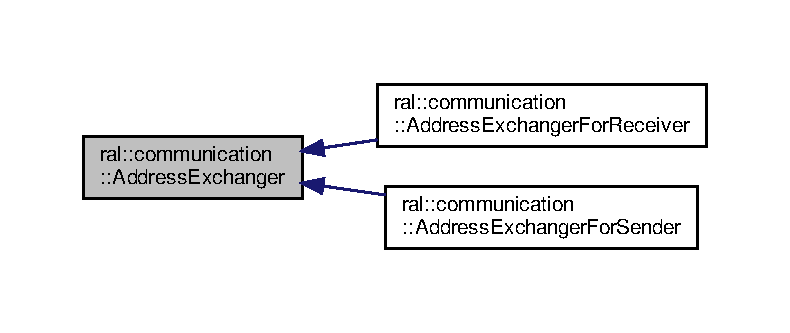
\includegraphics[width=350pt]{classral_1_1communication_1_1AddressExchanger__inherit__graph}
\end{center}
\end{figure}
\subsection*{Public Member Functions}
\begin{DoxyCompactItemize}
\item 
\mbox{\Hypertarget{classral_1_1communication_1_1AddressExchanger_a3bb71364f0c14281838adda5d6a90c5e}\label{classral_1_1communication_1_1AddressExchanger_a3bb71364f0c14281838adda5d6a90c5e}} 
const \hyperlink{classral_1_1communication_1_1UcpWorkerAddress}{Ucp\+Worker\+Address} {\bfseries Exchange} (const \hyperlink{classral_1_1communication_1_1UcpWorkerAddress}{Ucp\+Worker\+Address} \&ucp\+Worker\+Address)
\item 
\mbox{\Hypertarget{classral_1_1communication_1_1AddressExchanger_a471d68aeb123276a007fde516ae9bc15}\label{classral_1_1communication_1_1AddressExchanger_a471d68aeb123276a007fde516ae9bc15}} 
virtual int {\bfseries fd} ()=0
\end{DoxyCompactItemize}
\subsection*{Static Public Member Functions}
\begin{DoxyCompactItemize}
\item 
\mbox{\Hypertarget{classral_1_1communication_1_1AddressExchanger_ab976b52f00f63554e798d3372bdb8caf}\label{classral_1_1communication_1_1AddressExchanger_ab976b52f00f63554e798d3372bdb8caf}} 
static std\+::unique\+\_\+ptr$<$ \hyperlink{classral_1_1communication_1_1AddressExchanger}{Address\+Exchanger} $>$ {\bfseries Make\+For\+Sender} (const std\+::uint16\+\_\+t port)
\item 
\mbox{\Hypertarget{classral_1_1communication_1_1AddressExchanger_abbb8262eced0853ab6293def89f6ef87}\label{classral_1_1communication_1_1AddressExchanger_abbb8262eced0853ab6293def89f6ef87}} 
static std\+::unique\+\_\+ptr$<$ \hyperlink{classral_1_1communication_1_1AddressExchanger}{Address\+Exchanger} $>$ {\bfseries Make\+For\+Receiver} (const std\+::uint16\+\_\+t port, const char $\ast$hostname)
\end{DoxyCompactItemize}


The documentation for this class was generated from the following file\+:\begin{DoxyCompactItemize}
\item 
/home/tom/\+Documents/programming/romulo\+\_\+blazingsql/blazingsql/engine/src/communication/ucx\+\_\+init.\+h\end{DoxyCompactItemize}

\hypertarget{classral_1_1communication_1_1AddressExchangerForReceiver}{}\section{ral\+:\+:communication\+:\+:Address\+Exchanger\+For\+Receiver Class Reference}
\label{classral_1_1communication_1_1AddressExchangerForReceiver}\index{ral\+::communication\+::\+Address\+Exchanger\+For\+Receiver@{ral\+::communication\+::\+Address\+Exchanger\+For\+Receiver}}


Inheritance diagram for ral\+:\+:communication\+:\+:Address\+Exchanger\+For\+Receiver\+:\nopagebreak
\begin{figure}[H]
\begin{center}
\leavevmode
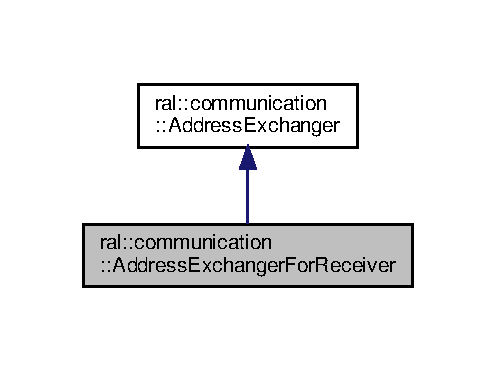
\includegraphics[width=238pt]{classral_1_1communication_1_1AddressExchangerForReceiver__inherit__graph}
\end{center}
\end{figure}


Collaboration diagram for ral\+:\+:communication\+:\+:Address\+Exchanger\+For\+Receiver\+:\nopagebreak
\begin{figure}[H]
\begin{center}
\leavevmode
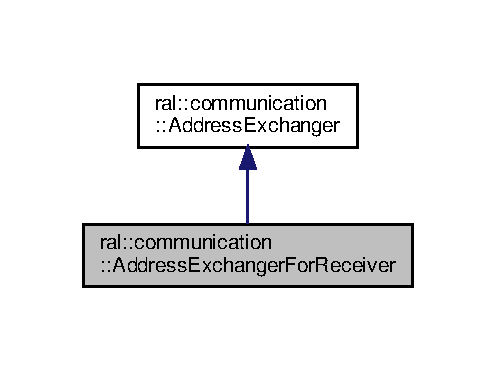
\includegraphics[width=238pt]{classral_1_1communication_1_1AddressExchangerForReceiver__coll__graph}
\end{center}
\end{figure}
\subsection*{Public Member Functions}
\begin{DoxyCompactItemize}
\item 
\mbox{\Hypertarget{classral_1_1communication_1_1AddressExchangerForReceiver_a4ba4be272f1c323187b1f4db91d08978}\label{classral_1_1communication_1_1AddressExchangerForReceiver_a4ba4be272f1c323187b1f4db91d08978}} 
{\bfseries Address\+Exchanger\+For\+Receiver} (const std\+::uint16\+\_\+t port, const char $\ast$hostname)
\item 
\mbox{\Hypertarget{classral_1_1communication_1_1AddressExchangerForReceiver_ac1b9066fdc95871b783dfae3c742df82}\label{classral_1_1communication_1_1AddressExchangerForReceiver_ac1b9066fdc95871b783dfae3c742df82}} 
int {\bfseries fd} () final
\end{DoxyCompactItemize}
\subsection*{Additional Inherited Members}


The documentation for this class was generated from the following file\+:\begin{DoxyCompactItemize}
\item 
/home/tom/\+Documents/programming/romulo\+\_\+blazingsql/blazingsql/engine/src/communication/ucx\+\_\+init.\+h\end{DoxyCompactItemize}

\hypertarget{classral_1_1communication_1_1AddressExchangerForSender}{}\section{ral\+:\+:communication\+:\+:Address\+Exchanger\+For\+Sender Class Reference}
\label{classral_1_1communication_1_1AddressExchangerForSender}\index{ral\+::communication\+::\+Address\+Exchanger\+For\+Sender@{ral\+::communication\+::\+Address\+Exchanger\+For\+Sender}}


Inheritance diagram for ral\+:\+:communication\+:\+:Address\+Exchanger\+For\+Sender\+:\nopagebreak
\begin{figure}[H]
\begin{center}
\leavevmode
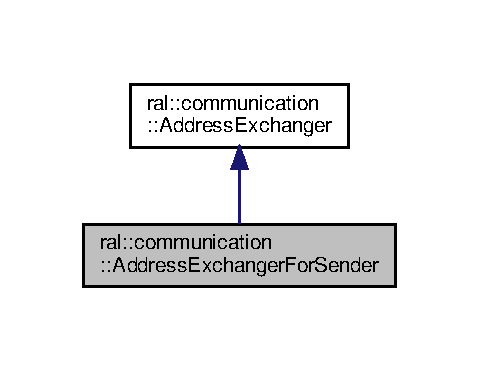
\includegraphics[width=230pt]{classral_1_1communication_1_1AddressExchangerForSender__inherit__graph}
\end{center}
\end{figure}


Collaboration diagram for ral\+:\+:communication\+:\+:Address\+Exchanger\+For\+Sender\+:\nopagebreak
\begin{figure}[H]
\begin{center}
\leavevmode
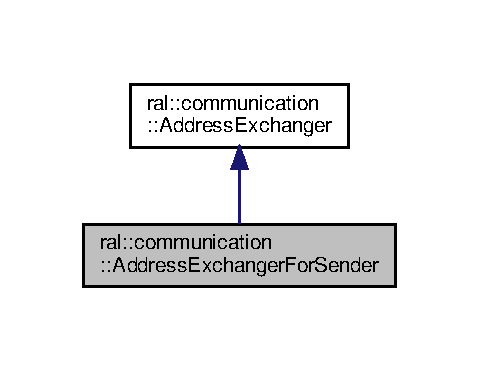
\includegraphics[width=230pt]{classral_1_1communication_1_1AddressExchangerForSender__coll__graph}
\end{center}
\end{figure}
\subsection*{Public Member Functions}
\begin{DoxyCompactItemize}
\item 
\mbox{\Hypertarget{classral_1_1communication_1_1AddressExchangerForSender_aed8329980dcfef4c782e0cd5cc23bc22}\label{classral_1_1communication_1_1AddressExchangerForSender_aed8329980dcfef4c782e0cd5cc23bc22}} 
{\bfseries Address\+Exchanger\+For\+Sender} (const std\+::uint16\+\_\+t port)
\item 
\mbox{\Hypertarget{classral_1_1communication_1_1AddressExchangerForSender_a90dff593f2b306ceb94940e213fda0bd}\label{classral_1_1communication_1_1AddressExchangerForSender_a90dff593f2b306ceb94940e213fda0bd}} 
char $\ast$ {\bfseries get\+\_\+ip\+\_\+str} (const struct sockaddr $\ast$sa, char $\ast$s, size\+\_\+t maxlen)
\item 
\mbox{\Hypertarget{classral_1_1communication_1_1AddressExchangerForSender_aca2eb6acefb439cd8d3b898d19d54d22}\label{classral_1_1communication_1_1AddressExchangerForSender_aca2eb6acefb439cd8d3b898d19d54d22}} 
bool {\bfseries accept\+Connection} ()
\item 
\mbox{\Hypertarget{classral_1_1communication_1_1AddressExchangerForSender_a5a2e5c7a53c81f6425aaaa4821f378ed}\label{classral_1_1communication_1_1AddressExchangerForSender_a5a2e5c7a53c81f6425aaaa4821f378ed}} 
void {\bfseries close\+Current\+Connection} ()
\item 
\mbox{\Hypertarget{classral_1_1communication_1_1AddressExchangerForSender_adaf94458ab22f538905644ff818be6f4}\label{classral_1_1communication_1_1AddressExchangerForSender_adaf94458ab22f538905644ff818be6f4}} 
int {\bfseries fd} () final
\end{DoxyCompactItemize}
\subsection*{Additional Inherited Members}


The documentation for this class was generated from the following file\+:\begin{DoxyCompactItemize}
\item 
/home/tom/\+Documents/programming/romulo\+\_\+blazingsql/blazingsql/engine/src/communication/ucx\+\_\+init.\+h\end{DoxyCompactItemize}

\hypertarget{classral_1_1memory_1_1allocation__pool}{}\section{ral\+:\+:memory\+:\+:allocation\+\_\+pool Class Reference}
\label{classral_1_1memory_1_1allocation__pool}\index{ral\+::memory\+::allocation\+\_\+pool@{ral\+::memory\+::allocation\+\_\+pool}}
\subsection*{Public Member Functions}
\begin{DoxyCompactItemize}
\item 
\mbox{\Hypertarget{classral_1_1memory_1_1allocation__pool_a7ca793ed2beca97009c7b9d280d3b8a5}\label{classral_1_1memory_1_1allocation__pool_a7ca793ed2beca97009c7b9d280d3b8a5}} 
{\bfseries allocation\+\_\+pool} (std\+::unique\+\_\+ptr$<$ \hyperlink{classral_1_1memory_1_1base__allocator}{base\+\_\+allocator} $>$ allocator, std\+::size\+\_\+t size\+\_\+buffers, std\+::size\+\_\+t num\+\_\+buffers)
\item 
\mbox{\Hypertarget{classral_1_1memory_1_1allocation__pool_a5494d7e758157816f90b62f77d9f09b0}\label{classral_1_1memory_1_1allocation__pool_a5494d7e758157816f90b62f77d9f09b0}} 
std\+::unique\+\_\+ptr$<$ \hyperlink{structral_1_1memory_1_1blazing__allocation__chunk}{blazing\+\_\+allocation\+\_\+chunk} $>$ {\bfseries get\+\_\+chunk} ()
\item 
\mbox{\Hypertarget{classral_1_1memory_1_1allocation__pool_a32240d0bf4c754e943db833d6979428b}\label{classral_1_1memory_1_1allocation__pool_a32240d0bf4c754e943db833d6979428b}} 
ucp\+\_\+mem\+\_\+h {\bfseries get\+Ucp\+Memory\+Handle} () const
\item 
\mbox{\Hypertarget{classral_1_1memory_1_1allocation__pool_a117316c8c3b893b49a013e1b795f5e4d}\label{classral_1_1memory_1_1allocation__pool_a117316c8c3b893b49a013e1b795f5e4d}} 
void {\bfseries free\+\_\+chunk} (std\+::unique\+\_\+ptr$<$ \hyperlink{structral_1_1memory_1_1blazing__allocation__chunk}{blazing\+\_\+allocation\+\_\+chunk} $>$ allocation)
\item 
\mbox{\Hypertarget{classral_1_1memory_1_1allocation__pool_a832314c575b0ecd133945738f07eb2e7}\label{classral_1_1memory_1_1allocation__pool_a832314c575b0ecd133945738f07eb2e7}} 
std\+::size\+\_\+t {\bfseries size\+\_\+buffers} ()
\item 
\mbox{\Hypertarget{classral_1_1memory_1_1allocation__pool_a891ab60c9c6756f91cd3c065885fcc98}\label{classral_1_1memory_1_1allocation__pool_a891ab60c9c6756f91cd3c065885fcc98}} 
void {\bfseries free\+\_\+all} ()
\item 
\mbox{\Hypertarget{classral_1_1memory_1_1allocation__pool_a736b458e329b20ff9f960f1948d71c48}\label{classral_1_1memory_1_1allocation__pool_a736b458e329b20ff9f960f1948d71c48}} 
std\+::size\+\_\+t {\bfseries get\+\_\+allocated\+\_\+buffers} ()
\item 
\mbox{\Hypertarget{classral_1_1memory_1_1allocation__pool_a75e28a2486e1eb1920a482a196612852}\label{classral_1_1memory_1_1allocation__pool_a75e28a2486e1eb1920a482a196612852}} 
std\+::size\+\_\+t {\bfseries get\+\_\+total\+\_\+buffers} ()
\end{DoxyCompactItemize}


The documentation for this class was generated from the following files\+:\begin{DoxyCompactItemize}
\item 
/home/tom/\+Documents/programming/romulo\+\_\+blazingsql/blazingsql/engine/src/bmr/Buffer\+Provider.\+h\item 
/home/tom/\+Documents/programming/romulo\+\_\+blazingsql/blazingsql/engine/src/bmr/Buffer\+Provider.\+cpp\end{DoxyCompactItemize}

\hypertarget{classral_1_1io_1_1arrow__parser}{}\section{ral\+:\+:io\+:\+:arrow\+\_\+parser Class Reference}
\label{classral_1_1io_1_1arrow__parser}\index{ral\+::io\+::arrow\+\_\+parser@{ral\+::io\+::arrow\+\_\+parser}}


Inheritance diagram for ral\+:\+:io\+:\+:arrow\+\_\+parser\+:\nopagebreak
\begin{figure}[H]
\begin{center}
\leavevmode
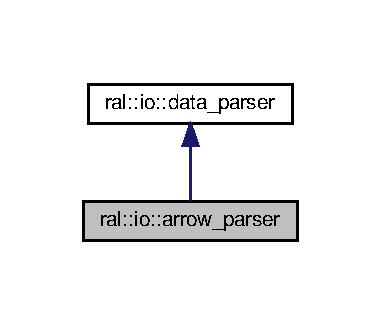
\includegraphics[width=183pt]{classral_1_1io_1_1arrow__parser__inherit__graph}
\end{center}
\end{figure}


Collaboration diagram for ral\+:\+:io\+:\+:arrow\+\_\+parser\+:\nopagebreak
\begin{figure}[H]
\begin{center}
\leavevmode
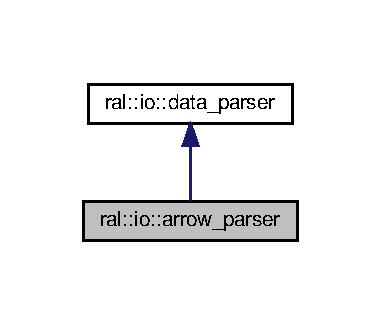
\includegraphics[width=183pt]{classral_1_1io_1_1arrow__parser__coll__graph}
\end{center}
\end{figure}
\subsection*{Public Member Functions}
\begin{DoxyCompactItemize}
\item 
\mbox{\Hypertarget{classral_1_1io_1_1arrow__parser_a6adb75628c932c35c5144323aed56204}\label{classral_1_1io_1_1arrow__parser_a6adb75628c932c35c5144323aed56204}} 
{\bfseries arrow\+\_\+parser} (std\+::shared\+\_\+ptr$<$ arrow\+::\+Table $>$ table)
\item 
\mbox{\Hypertarget{classral_1_1io_1_1arrow__parser_a64424836e1e59df80a393c77f31d1f2d}\label{classral_1_1io_1_1arrow__parser_a64424836e1e59df80a393c77f31d1f2d}} 
void {\bfseries parse\+\_\+schema} (std\+::shared\+\_\+ptr$<$ arrow\+::io\+::\+Random\+Access\+File $>$ file, \hyperlink{classral_1_1io_1_1Schema}{ral\+::io\+::\+Schema} \&schema)
\item 
\mbox{\Hypertarget{classral_1_1io_1_1arrow__parser_aa01d534dac941d08da9b4b9786e75ada}\label{classral_1_1io_1_1arrow__parser_aa01d534dac941d08da9b4b9786e75ada}} 
Data\+Type {\bfseries type} () const override
\end{DoxyCompactItemize}


The documentation for this class was generated from the following files\+:\begin{DoxyCompactItemize}
\item 
/home/tom/\+Documents/programming/romulo\+\_\+blazingsql/blazingsql/engine/src/io/data\+\_\+parser/Arrow\+Parser.\+h\item 
/home/tom/\+Documents/programming/romulo\+\_\+blazingsql/blazingsql/engine/src/io/data\+\_\+parser/Arrow\+Parser.\+cpp\end{DoxyCompactItemize}

\hypertarget{classral_1_1memory_1_1base__allocator}{}\section{ral\+:\+:memory\+:\+:base\+\_\+allocator Class Reference}
\label{classral_1_1memory_1_1base__allocator}\index{ral\+::memory\+::base\+\_\+allocator@{ral\+::memory\+::base\+\_\+allocator}}


Inheritance diagram for ral\+:\+:memory\+:\+:base\+\_\+allocator\+:\nopagebreak
\begin{figure}[H]
\begin{center}
\leavevmode
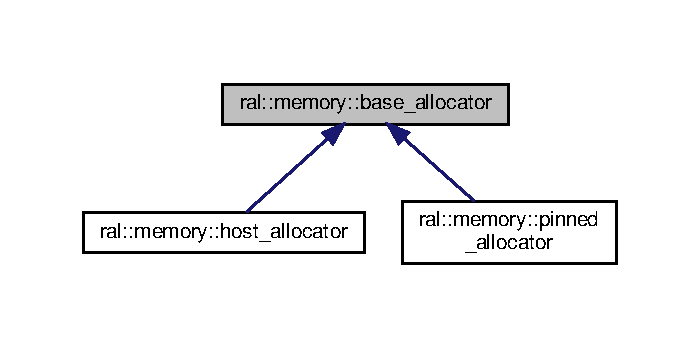
\includegraphics[width=336pt]{classral_1_1memory_1_1base__allocator__inherit__graph}
\end{center}
\end{figure}
\subsection*{Public Member Functions}
\begin{DoxyCompactItemize}
\item 
\mbox{\Hypertarget{classral_1_1memory_1_1base__allocator_af9f28272471b5c21700ec726703091db}\label{classral_1_1memory_1_1base__allocator_af9f28272471b5c21700ec726703091db}} 
void {\bfseries allocate} (void $\ast$$\ast$ptr, std\+::size\+\_\+t size)
\item 
\mbox{\Hypertarget{classral_1_1memory_1_1base__allocator_a5e5f35c397e7c906ca9e9c7b3aaaa473}\label{classral_1_1memory_1_1base__allocator_a5e5f35c397e7c906ca9e9c7b3aaaa473}} 
void {\bfseries deallocate} (void $\ast$ptr)
\item 
\mbox{\Hypertarget{classral_1_1memory_1_1base__allocator_a9be5143f73c55fc9b30b270ada544b01}\label{classral_1_1memory_1_1base__allocator_a9be5143f73c55fc9b30b270ada544b01}} 
virtual ucp\+\_\+mem\+\_\+h {\bfseries get\+Ucp\+Memory\+Handle} () const
\end{DoxyCompactItemize}
\subsection*{Protected Member Functions}
\begin{DoxyCompactItemize}
\item 
\mbox{\Hypertarget{classral_1_1memory_1_1base__allocator_ad6b8fa2aae326028c98fc36342b06ddc}\label{classral_1_1memory_1_1base__allocator_ad6b8fa2aae326028c98fc36342b06ddc}} 
virtual void {\bfseries do\+\_\+allocate} (void $\ast$$\ast$ptr, std\+::size\+\_\+t size)=0
\item 
\mbox{\Hypertarget{classral_1_1memory_1_1base__allocator_a934af0fdfb53ac5912e29e355580c703}\label{classral_1_1memory_1_1base__allocator_a934af0fdfb53ac5912e29e355580c703}} 
virtual void {\bfseries do\+\_\+deallocate} (void $\ast$ptr)=0
\end{DoxyCompactItemize}


The documentation for this class was generated from the following files\+:\begin{DoxyCompactItemize}
\item 
/home/tom/\+Documents/programming/romulo\+\_\+blazingsql/blazingsql/engine/src/bmr/Buffer\+Provider.\+h\item 
/home/tom/\+Documents/programming/romulo\+\_\+blazingsql/blazingsql/engine/src/bmr/Buffer\+Provider.\+cpp\end{DoxyCompactItemize}

\hypertarget{classral_1_1batch_1_1BatchSequence}{}\section{ral\+:\+:batch\+:\+:Batch\+Sequence Class Reference}
\label{classral_1_1batch_1_1BatchSequence}\index{ral\+::batch\+::\+Batch\+Sequence@{ral\+::batch\+::\+Batch\+Sequence}}


This is the standard data sequencer that just pulls data from an input cache one batch at a time.  




{\ttfamily \#include $<$Batch\+Processing.\+h$>$}

\subsection*{Public Member Functions}
\begin{DoxyCompactItemize}
\item 
\hyperlink{classral_1_1batch_1_1BatchSequence_a1012a9622924b621edd667400038b24d}{Batch\+Sequence} (std\+::shared\+\_\+ptr$<$ \hyperlink{classral_1_1cache_1_1CacheMachine}{ral\+::cache\+::\+Cache\+Machine} $>$ cache=nullptr, const \hyperlink{classral_1_1cache_1_1kernel}{ral\+::cache\+::kernel} $\ast$\hyperlink{classral_1_1cache_1_1kernel}{kernel}=nullptr, bool ordered=true)
\item 
void \hyperlink{classral_1_1batch_1_1BatchSequence_a92ce0d4e310caded265fceab3f4c266a}{set\+\_\+source} (std\+::shared\+\_\+ptr$<$ \hyperlink{classral_1_1cache_1_1CacheMachine}{ral\+::cache\+::\+Cache\+Machine} $>$ cache)
\item 
std\+::unique\+\_\+ptr$<$ \hyperlink{classral_1_1frame_1_1BlazingTable}{ral\+::frame\+::\+Blazing\+Table} $>$ \hyperlink{classral_1_1batch_1_1BatchSequence_a5fe181e6183df338739e61eb512c23a4}{next} ()
\item 
bool \hyperlink{classral_1_1batch_1_1BatchSequence_af62f1f620ac02a018737af8a89eb4881}{wait\+\_\+for\+\_\+next} ()
\item 
bool \hyperlink{classral_1_1batch_1_1BatchSequence_a0ed0531f11f65b4e7391da23c2a2de12}{has\+\_\+next\+\_\+now} ()
\end{DoxyCompactItemize}


\subsection{Detailed Description}
This is the standard data sequencer that just pulls data from an input cache one batch at a time. 

\subsection{Constructor \& Destructor Documentation}
\mbox{\Hypertarget{classral_1_1batch_1_1BatchSequence_a1012a9622924b621edd667400038b24d}\label{classral_1_1batch_1_1BatchSequence_a1012a9622924b621edd667400038b24d}} 
\index{ral\+::batch\+::\+Batch\+Sequence@{ral\+::batch\+::\+Batch\+Sequence}!Batch\+Sequence@{Batch\+Sequence}}
\index{Batch\+Sequence@{Batch\+Sequence}!ral\+::batch\+::\+Batch\+Sequence@{ral\+::batch\+::\+Batch\+Sequence}}
\subsubsection{\texorpdfstring{Batch\+Sequence()}{BatchSequence()}}
{\footnotesize\ttfamily ral\+::batch\+::\+Batch\+Sequence\+::\+Batch\+Sequence (\begin{DoxyParamCaption}\item[{std\+::shared\+\_\+ptr$<$ \hyperlink{classral_1_1cache_1_1CacheMachine}{ral\+::cache\+::\+Cache\+Machine} $>$}]{cache = {\ttfamily nullptr},  }\item[{const \hyperlink{classral_1_1cache_1_1kernel}{ral\+::cache\+::kernel} $\ast$}]{kernel = {\ttfamily nullptr},  }\item[{bool}]{ordered = {\ttfamily true} }\end{DoxyParamCaption})}

Constructor for the \hyperlink{classral_1_1batch_1_1BatchSequence}{Batch\+Sequence} 
\begin{DoxyParams}{Parameters}
{\em cache} & The input cache from where the data will be pulled. \\
\hline
{\em kernel} & The kernel that will actually receive the pulled data. \\
\hline
{\em ordered} & Indicates whether the order should be kept at data pulling. \\
\hline
\end{DoxyParams}


\subsection{Member Function Documentation}
\mbox{\Hypertarget{classral_1_1batch_1_1BatchSequence_a0ed0531f11f65b4e7391da23c2a2de12}\label{classral_1_1batch_1_1BatchSequence_a0ed0531f11f65b4e7391da23c2a2de12}} 
\index{ral\+::batch\+::\+Batch\+Sequence@{ral\+::batch\+::\+Batch\+Sequence}!has\+\_\+next\+\_\+now@{has\+\_\+next\+\_\+now}}
\index{has\+\_\+next\+\_\+now@{has\+\_\+next\+\_\+now}!ral\+::batch\+::\+Batch\+Sequence@{ral\+::batch\+::\+Batch\+Sequence}}
\subsubsection{\texorpdfstring{has\+\_\+next\+\_\+now()}{has\_next\_now()}}
{\footnotesize\ttfamily bool ral\+::batch\+::\+Batch\+Sequence\+::has\+\_\+next\+\_\+now (\begin{DoxyParamCaption}{ }\end{DoxyParamCaption})}

Indicates if the message queue is not empty at this point on time. \begin{DoxyReturn}{Returns}
true There is at least one message in the queue. 

false Message queue is empty. 
\end{DoxyReturn}
\mbox{\Hypertarget{classral_1_1batch_1_1BatchSequence_a5fe181e6183df338739e61eb512c23a4}\label{classral_1_1batch_1_1BatchSequence_a5fe181e6183df338739e61eb512c23a4}} 
\index{ral\+::batch\+::\+Batch\+Sequence@{ral\+::batch\+::\+Batch\+Sequence}!next@{next}}
\index{next@{next}!ral\+::batch\+::\+Batch\+Sequence@{ral\+::batch\+::\+Batch\+Sequence}}
\subsubsection{\texorpdfstring{next()}{next()}}
{\footnotesize\ttfamily std\+::unique\+\_\+ptr$<$ \hyperlink{classral_1_1frame_1_1BlazingTable}{ral\+::frame\+::\+Blazing\+Table} $>$ ral\+::batch\+::\+Batch\+Sequence\+::next (\begin{DoxyParamCaption}{ }\end{DoxyParamCaption})}

Get the next message as a unique pointer to a Blazing\+Table. If there are no more messages on the queue we get a nullptr. \begin{DoxyReturn}{Returns}
Unique pointer to a Blazing\+Table containing the next decached message. 
\end{DoxyReturn}
Here is the caller graph for this function\+:\nopagebreak
\begin{figure}[H]
\begin{center}
\leavevmode
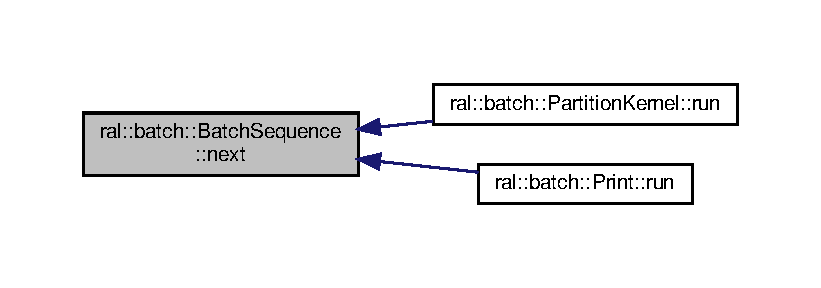
\includegraphics[width=350pt]{classral_1_1batch_1_1BatchSequence_a5fe181e6183df338739e61eb512c23a4_icgraph}
\end{center}
\end{figure}
\mbox{\Hypertarget{classral_1_1batch_1_1BatchSequence_a92ce0d4e310caded265fceab3f4c266a}\label{classral_1_1batch_1_1BatchSequence_a92ce0d4e310caded265fceab3f4c266a}} 
\index{ral\+::batch\+::\+Batch\+Sequence@{ral\+::batch\+::\+Batch\+Sequence}!set\+\_\+source@{set\+\_\+source}}
\index{set\+\_\+source@{set\+\_\+source}!ral\+::batch\+::\+Batch\+Sequence@{ral\+::batch\+::\+Batch\+Sequence}}
\subsubsection{\texorpdfstring{set\+\_\+source()}{set\_source()}}
{\footnotesize\ttfamily void ral\+::batch\+::\+Batch\+Sequence\+::set\+\_\+source (\begin{DoxyParamCaption}\item[{std\+::shared\+\_\+ptr$<$ \hyperlink{classral_1_1cache_1_1CacheMachine}{ral\+::cache\+::\+Cache\+Machine} $>$}]{cache }\end{DoxyParamCaption})}

Updates the input cache machine. 
\begin{DoxyParams}{Parameters}
{\em cache} & The pointer to the new input cache. \\
\hline
\end{DoxyParams}
\mbox{\Hypertarget{classral_1_1batch_1_1BatchSequence_af62f1f620ac02a018737af8a89eb4881}\label{classral_1_1batch_1_1BatchSequence_af62f1f620ac02a018737af8a89eb4881}} 
\index{ral\+::batch\+::\+Batch\+Sequence@{ral\+::batch\+::\+Batch\+Sequence}!wait\+\_\+for\+\_\+next@{wait\+\_\+for\+\_\+next}}
\index{wait\+\_\+for\+\_\+next@{wait\+\_\+for\+\_\+next}!ral\+::batch\+::\+Batch\+Sequence@{ral\+::batch\+::\+Batch\+Sequence}}
\subsubsection{\texorpdfstring{wait\+\_\+for\+\_\+next()}{wait\_for\_next()}}
{\footnotesize\ttfamily bool ral\+::batch\+::\+Batch\+Sequence\+::wait\+\_\+for\+\_\+next (\begin{DoxyParamCaption}{ }\end{DoxyParamCaption})}

Blocks executing thread until a new message is ready or when the message queue is empty. \begin{DoxyReturn}{Returns}
true A new message is ready. 

false There are no more messages on the cache. 
\end{DoxyReturn}
Here is the call graph for this function\+:\nopagebreak
\begin{figure}[H]
\begin{center}
\leavevmode
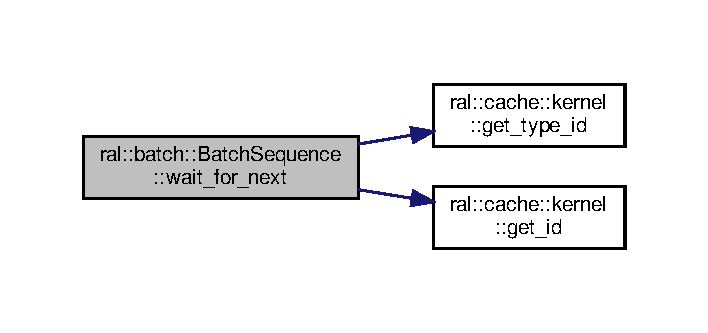
\includegraphics[width=340pt]{classral_1_1batch_1_1BatchSequence_af62f1f620ac02a018737af8a89eb4881_cgraph}
\end{center}
\end{figure}
Here is the caller graph for this function\+:\nopagebreak
\begin{figure}[H]
\begin{center}
\leavevmode
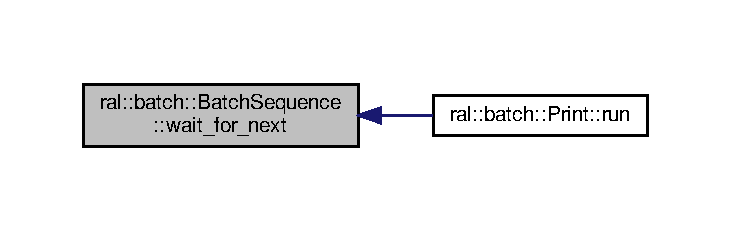
\includegraphics[width=350pt]{classral_1_1batch_1_1BatchSequence_af62f1f620ac02a018737af8a89eb4881_icgraph}
\end{center}
\end{figure}


The documentation for this class was generated from the following files\+:\begin{DoxyCompactItemize}
\item 
/home/tom/\+Documents/programming/romulo\+\_\+blazingsql/blazingsql/engine/src/execution\+\_\+graph/logic\+\_\+controllers/Batch\+Processing.\+h\item 
/home/tom/\+Documents/programming/romulo\+\_\+blazingsql/blazingsql/engine/src/execution\+\_\+graph/logic\+\_\+controllers/Batch\+Processing.\+cpp\end{DoxyCompactItemize}

\hypertarget{classral_1_1batch_1_1BatchSequenceBypass}{}\section{ral\+:\+:batch\+:\+:Batch\+Sequence\+Bypass Class Reference}
\label{classral_1_1batch_1_1BatchSequenceBypass}\index{ral\+::batch\+::\+Batch\+Sequence\+Bypass@{ral\+::batch\+::\+Batch\+Sequence\+Bypass}}


This data sequencer works as a bypass to take data from one input to an output without decacheing.  




{\ttfamily \#include $<$Batch\+Processing.\+h$>$}

\subsection*{Public Member Functions}
\begin{DoxyCompactItemize}
\item 
\hyperlink{classral_1_1batch_1_1BatchSequenceBypass_aece145bb27dd1aa61252a831b8d0b536}{Batch\+Sequence\+Bypass} (std\+::shared\+\_\+ptr$<$ \hyperlink{classral_1_1cache_1_1CacheMachine}{ral\+::cache\+::\+Cache\+Machine} $>$ cache=nullptr, const \hyperlink{classral_1_1cache_1_1kernel}{ral\+::cache\+::kernel} $\ast$\hyperlink{classral_1_1cache_1_1kernel}{kernel}=nullptr)
\item 
void \hyperlink{classral_1_1batch_1_1BatchSequenceBypass_aaf3b8397046f0ad622a49c751861d983}{set\+\_\+source} (std\+::shared\+\_\+ptr$<$ \hyperlink{classral_1_1cache_1_1CacheMachine}{ral\+::cache\+::\+Cache\+Machine} $>$ cache)
\item 
std\+::unique\+\_\+ptr$<$ \hyperlink{classral_1_1cache_1_1CacheData}{ral\+::cache\+::\+Cache\+Data} $>$ \hyperlink{classral_1_1batch_1_1BatchSequenceBypass_a5d55f785961b21c82578223ab5a0a217}{next} ()
\item 
bool \hyperlink{classral_1_1batch_1_1BatchSequenceBypass_a623422aa9164a34bce024e92f4f26679}{wait\+\_\+for\+\_\+next} ()
\item 
bool \hyperlink{classral_1_1batch_1_1BatchSequenceBypass_a221ad94710394f83ebbeeabcc1851b22}{has\+\_\+next\+\_\+now} ()
\end{DoxyCompactItemize}


\subsection{Detailed Description}
This data sequencer works as a bypass to take data from one input to an output without decacheing. 

\subsection{Constructor \& Destructor Documentation}
\mbox{\Hypertarget{classral_1_1batch_1_1BatchSequenceBypass_aece145bb27dd1aa61252a831b8d0b536}\label{classral_1_1batch_1_1BatchSequenceBypass_aece145bb27dd1aa61252a831b8d0b536}} 
\index{ral\+::batch\+::\+Batch\+Sequence\+Bypass@{ral\+::batch\+::\+Batch\+Sequence\+Bypass}!Batch\+Sequence\+Bypass@{Batch\+Sequence\+Bypass}}
\index{Batch\+Sequence\+Bypass@{Batch\+Sequence\+Bypass}!ral\+::batch\+::\+Batch\+Sequence\+Bypass@{ral\+::batch\+::\+Batch\+Sequence\+Bypass}}
\subsubsection{\texorpdfstring{Batch\+Sequence\+Bypass()}{BatchSequenceBypass()}}
{\footnotesize\ttfamily ral\+::batch\+::\+Batch\+Sequence\+Bypass\+::\+Batch\+Sequence\+Bypass (\begin{DoxyParamCaption}\item[{std\+::shared\+\_\+ptr$<$ \hyperlink{classral_1_1cache_1_1CacheMachine}{ral\+::cache\+::\+Cache\+Machine} $>$}]{cache = {\ttfamily nullptr},  }\item[{const \hyperlink{classral_1_1cache_1_1kernel}{ral\+::cache\+::kernel} $\ast$}]{kernel = {\ttfamily nullptr} }\end{DoxyParamCaption})}

Constructor for the \hyperlink{classral_1_1batch_1_1BatchSequenceBypass}{Batch\+Sequence\+Bypass} 
\begin{DoxyParams}{Parameters}
{\em cache} & The input cache from where the data will be pulled. \\
\hline
{\em kernel} & The kernel that will actually receive the pulled data. \\
\hline
\end{DoxyParams}


\subsection{Member Function Documentation}
\mbox{\Hypertarget{classral_1_1batch_1_1BatchSequenceBypass_a221ad94710394f83ebbeeabcc1851b22}\label{classral_1_1batch_1_1BatchSequenceBypass_a221ad94710394f83ebbeeabcc1851b22}} 
\index{ral\+::batch\+::\+Batch\+Sequence\+Bypass@{ral\+::batch\+::\+Batch\+Sequence\+Bypass}!has\+\_\+next\+\_\+now@{has\+\_\+next\+\_\+now}}
\index{has\+\_\+next\+\_\+now@{has\+\_\+next\+\_\+now}!ral\+::batch\+::\+Batch\+Sequence\+Bypass@{ral\+::batch\+::\+Batch\+Sequence\+Bypass}}
\subsubsection{\texorpdfstring{has\+\_\+next\+\_\+now()}{has\_next\_now()}}
{\footnotesize\ttfamily bool ral\+::batch\+::\+Batch\+Sequence\+Bypass\+::has\+\_\+next\+\_\+now (\begin{DoxyParamCaption}{ }\end{DoxyParamCaption})}

Indicates if the message queue is not empty at this point on time. \begin{DoxyReturn}{Returns}
true There is at least one message in the queue. 

false Message queue is empty. 
\end{DoxyReturn}
\mbox{\Hypertarget{classral_1_1batch_1_1BatchSequenceBypass_a5d55f785961b21c82578223ab5a0a217}\label{classral_1_1batch_1_1BatchSequenceBypass_a5d55f785961b21c82578223ab5a0a217}} 
\index{ral\+::batch\+::\+Batch\+Sequence\+Bypass@{ral\+::batch\+::\+Batch\+Sequence\+Bypass}!next@{next}}
\index{next@{next}!ral\+::batch\+::\+Batch\+Sequence\+Bypass@{ral\+::batch\+::\+Batch\+Sequence\+Bypass}}
\subsubsection{\texorpdfstring{next()}{next()}}
{\footnotesize\ttfamily std\+::unique\+\_\+ptr$<$ \hyperlink{classral_1_1cache_1_1CacheData}{ral\+::cache\+::\+Cache\+Data} $>$ ral\+::batch\+::\+Batch\+Sequence\+Bypass\+::next (\begin{DoxyParamCaption}{ }\end{DoxyParamCaption})}

Get the next message as a Cache\+Data object. \begin{DoxyReturn}{Returns}
Cache\+Data containing the next message without decacheing. 
\end{DoxyReturn}
Here is the caller graph for this function\+:\nopagebreak
\begin{figure}[H]
\begin{center}
\leavevmode
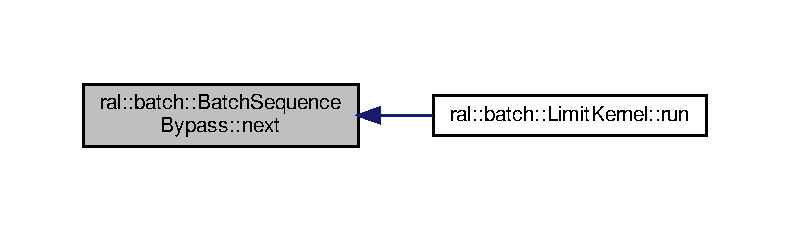
\includegraphics[width=350pt]{classral_1_1batch_1_1BatchSequenceBypass_a5d55f785961b21c82578223ab5a0a217_icgraph}
\end{center}
\end{figure}
\mbox{\Hypertarget{classral_1_1batch_1_1BatchSequenceBypass_aaf3b8397046f0ad622a49c751861d983}\label{classral_1_1batch_1_1BatchSequenceBypass_aaf3b8397046f0ad622a49c751861d983}} 
\index{ral\+::batch\+::\+Batch\+Sequence\+Bypass@{ral\+::batch\+::\+Batch\+Sequence\+Bypass}!set\+\_\+source@{set\+\_\+source}}
\index{set\+\_\+source@{set\+\_\+source}!ral\+::batch\+::\+Batch\+Sequence\+Bypass@{ral\+::batch\+::\+Batch\+Sequence\+Bypass}}
\subsubsection{\texorpdfstring{set\+\_\+source()}{set\_source()}}
{\footnotesize\ttfamily void ral\+::batch\+::\+Batch\+Sequence\+Bypass\+::set\+\_\+source (\begin{DoxyParamCaption}\item[{std\+::shared\+\_\+ptr$<$ \hyperlink{classral_1_1cache_1_1CacheMachine}{ral\+::cache\+::\+Cache\+Machine} $>$}]{cache }\end{DoxyParamCaption})}

Updates the input cache machine. 
\begin{DoxyParams}{Parameters}
{\em cache} & The pointer to the new input cache. \\
\hline
\end{DoxyParams}
\mbox{\Hypertarget{classral_1_1batch_1_1BatchSequenceBypass_a623422aa9164a34bce024e92f4f26679}\label{classral_1_1batch_1_1BatchSequenceBypass_a623422aa9164a34bce024e92f4f26679}} 
\index{ral\+::batch\+::\+Batch\+Sequence\+Bypass@{ral\+::batch\+::\+Batch\+Sequence\+Bypass}!wait\+\_\+for\+\_\+next@{wait\+\_\+for\+\_\+next}}
\index{wait\+\_\+for\+\_\+next@{wait\+\_\+for\+\_\+next}!ral\+::batch\+::\+Batch\+Sequence\+Bypass@{ral\+::batch\+::\+Batch\+Sequence\+Bypass}}
\subsubsection{\texorpdfstring{wait\+\_\+for\+\_\+next()}{wait\_for\_next()}}
{\footnotesize\ttfamily bool ral\+::batch\+::\+Batch\+Sequence\+Bypass\+::wait\+\_\+for\+\_\+next (\begin{DoxyParamCaption}{ }\end{DoxyParamCaption})}

Blocks executing thread until a new message is ready or when the message queue is empty. \begin{DoxyReturn}{Returns}
true A new message is ready. 

false There are no more messages on the cache. 
\end{DoxyReturn}
Here is the caller graph for this function\+:\nopagebreak
\begin{figure}[H]
\begin{center}
\leavevmode
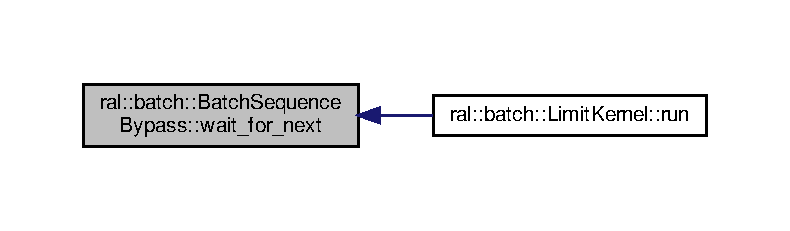
\includegraphics[width=350pt]{classral_1_1batch_1_1BatchSequenceBypass_a623422aa9164a34bce024e92f4f26679_icgraph}
\end{center}
\end{figure}


The documentation for this class was generated from the following files\+:\begin{DoxyCompactItemize}
\item 
/home/tom/\+Documents/programming/romulo\+\_\+blazingsql/blazingsql/engine/src/execution\+\_\+graph/logic\+\_\+controllers/Batch\+Processing.\+h\item 
/home/tom/\+Documents/programming/romulo\+\_\+blazingsql/blazingsql/engine/src/execution\+\_\+graph/logic\+\_\+controllers/Batch\+Processing.\+cpp\end{DoxyCompactItemize}

\hypertarget{classral_1_1batch_1_1BindableTableScan}{}\section{ral\+:\+:batch\+:\+:Bindable\+Table\+Scan Class Reference}
\label{classral_1_1batch_1_1BindableTableScan}\index{ral\+::batch\+::\+Bindable\+Table\+Scan@{ral\+::batch\+::\+Bindable\+Table\+Scan}}


This kernel loads the data and delivers only columns that are requested. It also filters the data if there are one or more filters, and sets their column aliases accordingly.  




{\ttfamily \#include $<$Batch\+Processing.\+h$>$}



Inheritance diagram for ral\+:\+:batch\+:\+:Bindable\+Table\+Scan\+:\nopagebreak
\begin{figure}[H]
\begin{center}
\leavevmode
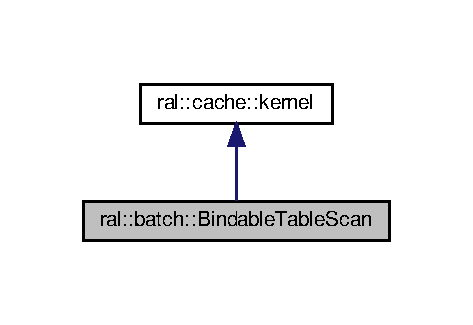
\includegraphics[width=227pt]{classral_1_1batch_1_1BindableTableScan__inherit__graph}
\end{center}
\end{figure}


Collaboration diagram for ral\+:\+:batch\+:\+:Bindable\+Table\+Scan\+:\nopagebreak
\begin{figure}[H]
\begin{center}
\leavevmode
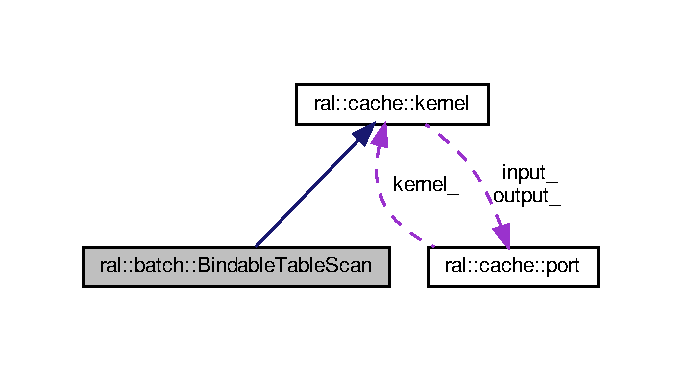
\includegraphics[width=328pt]{classral_1_1batch_1_1BindableTableScan__coll__graph}
\end{center}
\end{figure}
\subsection*{Public Member Functions}
\begin{DoxyCompactItemize}
\item 
\hyperlink{classral_1_1batch_1_1BindableTableScan_adc92c38cd526bfbf6b1586fbfa4058cc}{Bindable\+Table\+Scan} (std\+::size\+\_\+t \hyperlink{classral_1_1cache_1_1kernel_a2fd708656cb056a41ec635b8bdc4acfe}{kernel\+\_\+id}, const std\+::string \&query\+String, std\+::shared\+\_\+ptr$<$ \hyperlink{classral_1_1io_1_1data__provider}{ral\+::io\+::data\+\_\+provider} $>$ provider, std\+::shared\+\_\+ptr$<$ \hyperlink{classral_1_1io_1_1data__parser}{ral\+::io\+::data\+\_\+parser} $>$ parser, \hyperlink{classral_1_1io_1_1Schema}{ral\+::io\+::\+Schema} \&schema, std\+::shared\+\_\+ptr$<$ \hyperlink{classblazingdb_1_1manager_1_1Context}{Context} $>$ \hyperlink{classral_1_1cache_1_1kernel_af0347d14d678cfa7205c1387746a2e1b}{context}, std\+::shared\+\_\+ptr$<$ \hyperlink{classral_1_1cache_1_1graph}{ral\+::cache\+::graph} $>$ \hyperlink{classral_1_1cache_1_1kernel_a5fbb02292aff165a28ef25e75f0d89bd}{query\+\_\+graph})
\item 
\mbox{\Hypertarget{classral_1_1batch_1_1BindableTableScan_a0a83091e678279f9de802ec8856ca705}\label{classral_1_1batch_1_1BindableTableScan_a0a83091e678279f9de802ec8856ca705}} 
std\+::string {\bfseries kernel\+\_\+name} ()
\item 
\mbox{\Hypertarget{classral_1_1batch_1_1BindableTableScan_abe5282c1203677b2c02dde35f122416c}\label{classral_1_1batch_1_1BindableTableScan_abe5282c1203677b2c02dde35f122416c}} 
\hyperlink{structral_1_1execution_1_1task__result}{ral\+::execution\+::task\+\_\+result} {\bfseries do\+\_\+process} (std\+::vector$<$ std\+::unique\+\_\+ptr$<$ \hyperlink{classral_1_1frame_1_1BlazingTable}{ral\+::frame\+::\+Blazing\+Table} $>$ $>$ inputs, std\+::shared\+\_\+ptr$<$ \hyperlink{classral_1_1cache_1_1CacheMachine}{ral\+::cache\+::\+Cache\+Machine} $>$ output, cuda\+Stream\+\_\+t stream, const std\+::map$<$ std\+::string, std\+::string $>$ \&args) override
\item 
kstatus \hyperlink{classral_1_1batch_1_1BindableTableScan_a3215b390c1b588e165724b108038cbf9}{run} () override
\item 
std\+::pair$<$ bool, uint64\+\_\+t $>$ \hyperlink{classral_1_1batch_1_1BindableTableScan_aa5054a845227c869fd27869e1784eb4d}{get\+\_\+estimated\+\_\+output\+\_\+num\+\_\+rows} () override
\end{DoxyCompactItemize}
\subsection*{Additional Inherited Members}


\subsection{Detailed Description}
This kernel loads the data and delivers only columns that are requested. It also filters the data if there are one or more filters, and sets their column aliases accordingly. 

\subsection{Constructor \& Destructor Documentation}
\mbox{\Hypertarget{classral_1_1batch_1_1BindableTableScan_adc92c38cd526bfbf6b1586fbfa4058cc}\label{classral_1_1batch_1_1BindableTableScan_adc92c38cd526bfbf6b1586fbfa4058cc}} 
\index{ral\+::batch\+::\+Bindable\+Table\+Scan@{ral\+::batch\+::\+Bindable\+Table\+Scan}!Bindable\+Table\+Scan@{Bindable\+Table\+Scan}}
\index{Bindable\+Table\+Scan@{Bindable\+Table\+Scan}!ral\+::batch\+::\+Bindable\+Table\+Scan@{ral\+::batch\+::\+Bindable\+Table\+Scan}}
\subsubsection{\texorpdfstring{Bindable\+Table\+Scan()}{BindableTableScan()}}
{\footnotesize\ttfamily ral\+::batch\+::\+Bindable\+Table\+Scan\+::\+Bindable\+Table\+Scan (\begin{DoxyParamCaption}\item[{std\+::size\+\_\+t}]{kernel\+\_\+id,  }\item[{const std\+::string \&}]{query\+String,  }\item[{std\+::shared\+\_\+ptr$<$ \hyperlink{classral_1_1io_1_1data__provider}{ral\+::io\+::data\+\_\+provider} $>$}]{provider,  }\item[{std\+::shared\+\_\+ptr$<$ \hyperlink{classral_1_1io_1_1data__parser}{ral\+::io\+::data\+\_\+parser} $>$}]{parser,  }\item[{\hyperlink{classral_1_1io_1_1Schema}{ral\+::io\+::\+Schema} \&}]{schema,  }\item[{std\+::shared\+\_\+ptr$<$ \hyperlink{classblazingdb_1_1manager_1_1Context}{Context} $>$}]{context,  }\item[{std\+::shared\+\_\+ptr$<$ \hyperlink{classral_1_1cache_1_1graph}{ral\+::cache\+::graph} $>$}]{query\+\_\+graph }\end{DoxyParamCaption})}

Constructor for \hyperlink{classral_1_1batch_1_1BindableTableScan}{Bindable\+Table\+Scan} 
\begin{DoxyParams}{Parameters}
{\em kernel\+\_\+id} & Kernel identifier. \\
\hline
{\em query\+String} & Original logical expression that the kernel will execute. \\
\hline
{\em loader} & Data loader responsible for executing the batching load. \\
\hline
{\em schema} & Table schema associated to the data to be loaded. \\
\hline
{\em context} & Shared context associated to the running query. \\
\hline
{\em query\+\_\+graph} & Shared pointer of the current execution graph. \\
\hline
\end{DoxyParams}


\subsection{Member Function Documentation}
\mbox{\Hypertarget{classral_1_1batch_1_1BindableTableScan_aa5054a845227c869fd27869e1784eb4d}\label{classral_1_1batch_1_1BindableTableScan_aa5054a845227c869fd27869e1784eb4d}} 
\index{ral\+::batch\+::\+Bindable\+Table\+Scan@{ral\+::batch\+::\+Bindable\+Table\+Scan}!get\+\_\+estimated\+\_\+output\+\_\+num\+\_\+rows@{get\+\_\+estimated\+\_\+output\+\_\+num\+\_\+rows}}
\index{get\+\_\+estimated\+\_\+output\+\_\+num\+\_\+rows@{get\+\_\+estimated\+\_\+output\+\_\+num\+\_\+rows}!ral\+::batch\+::\+Bindable\+Table\+Scan@{ral\+::batch\+::\+Bindable\+Table\+Scan}}
\subsubsection{\texorpdfstring{get\+\_\+estimated\+\_\+output\+\_\+num\+\_\+rows()}{get\_estimated\_output\_num\_rows()}}
{\footnotesize\ttfamily std\+::pair$<$ bool, uint64\+\_\+t $>$ ral\+::batch\+::\+Bindable\+Table\+Scan\+::get\+\_\+estimated\+\_\+output\+\_\+num\+\_\+rows (\begin{DoxyParamCaption}{ }\end{DoxyParamCaption})\hspace{0.3cm}{\ttfamily [override]}, {\ttfamily [virtual]}}

Returns the estimated num\+\_\+rows for the output at one point. \begin{DoxyReturn}{Returns}
A pair representing that there is no data to be processed, or the estimated number of output rows. 
\end{DoxyReturn}


Reimplemented from \hyperlink{classral_1_1cache_1_1kernel_abf40aaa022e3bf38c261977d0c2170cb}{ral\+::cache\+::kernel}.

\mbox{\Hypertarget{classral_1_1batch_1_1BindableTableScan_a3215b390c1b588e165724b108038cbf9}\label{classral_1_1batch_1_1BindableTableScan_a3215b390c1b588e165724b108038cbf9}} 
\index{ral\+::batch\+::\+Bindable\+Table\+Scan@{ral\+::batch\+::\+Bindable\+Table\+Scan}!run@{run}}
\index{run@{run}!ral\+::batch\+::\+Bindable\+Table\+Scan@{ral\+::batch\+::\+Bindable\+Table\+Scan}}
\subsubsection{\texorpdfstring{run()}{run()}}
{\footnotesize\ttfamily kstatus ral\+::batch\+::\+Bindable\+Table\+Scan\+::run (\begin{DoxyParamCaption}{ }\end{DoxyParamCaption})\hspace{0.3cm}{\ttfamily [override]}, {\ttfamily [virtual]}}

Executes the batch processing. Loads the data from their input port, and after processing it, the results are stored in their output port. \begin{DoxyReturn}{Returns}
kstatus \textquotesingle{}stop\textquotesingle{} to halt processing, or \textquotesingle{}proceed\textquotesingle{} to continue processing. 
\end{DoxyReturn}


Implements \hyperlink{classral_1_1cache_1_1kernel_a735b081cccae9574924e74ea6d293ef7}{ral\+::cache\+::kernel}.

Here is the call graph for this function\+:\nopagebreak
\begin{figure}[H]
\begin{center}
\leavevmode
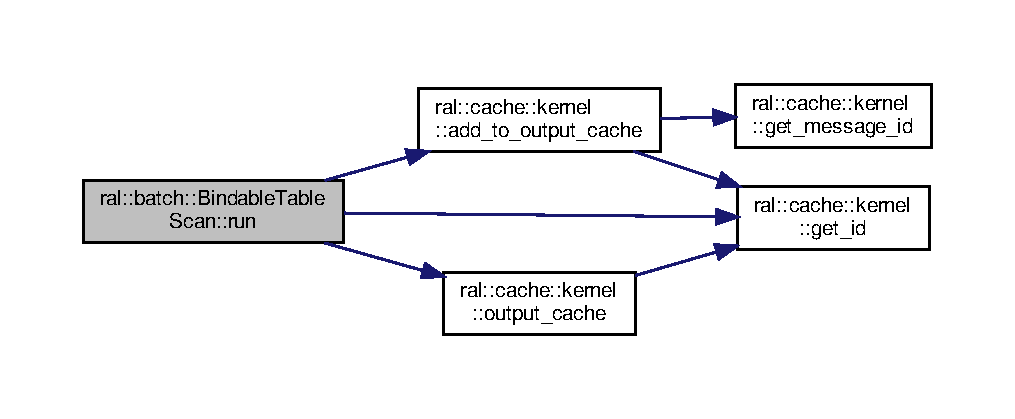
\includegraphics[width=350pt]{classral_1_1batch_1_1BindableTableScan_a3215b390c1b588e165724b108038cbf9_cgraph}
\end{center}
\end{figure}


The documentation for this class was generated from the following files\+:\begin{DoxyCompactItemize}
\item 
/home/tom/\+Documents/programming/romulo\+\_\+blazingsql/blazingsql/engine/src/execution\+\_\+graph/logic\+\_\+controllers/Batch\+Processing.\+h\item 
/home/tom/\+Documents/programming/romulo\+\_\+blazingsql/blazingsql/engine/src/execution\+\_\+graph/logic\+\_\+controllers/Batch\+Processing.\+cpp\end{DoxyCompactItemize}

\hypertarget{structral_1_1memory_1_1blazing__allocation}{}\section{ral\+:\+:memory\+:\+:blazing\+\_\+allocation Struct Reference}
\label{structral_1_1memory_1_1blazing__allocation}\index{ral\+::memory\+::blazing\+\_\+allocation@{ral\+::memory\+::blazing\+\_\+allocation}}


Collaboration diagram for ral\+:\+:memory\+:\+:blazing\+\_\+allocation\+:\nopagebreak
\begin{figure}[H]
\begin{center}
\leavevmode
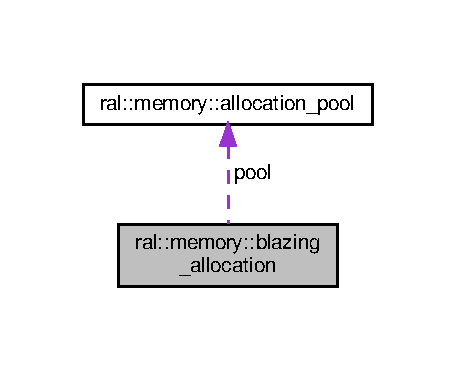
\includegraphics[width=219pt]{structral_1_1memory_1_1blazing__allocation__coll__graph}
\end{center}
\end{figure}
\subsection*{Public Attributes}
\begin{DoxyCompactItemize}
\item 
\mbox{\Hypertarget{structral_1_1memory_1_1blazing__allocation_a5ba48f9dbefe7e168f957ad776ba3d6a}\label{structral_1_1memory_1_1blazing__allocation_a5ba48f9dbefe7e168f957ad776ba3d6a}} 
std\+::size\+\_\+t {\bfseries index}
\item 
\mbox{\Hypertarget{structral_1_1memory_1_1blazing__allocation_a04163d566f783651e8a093e629042cf6}\label{structral_1_1memory_1_1blazing__allocation_a04163d566f783651e8a093e629042cf6}} 
std\+::size\+\_\+t {\bfseries size}
\item 
\mbox{\Hypertarget{structral_1_1memory_1_1blazing__allocation_abacfe2133dc90c845045f64ebc3b03d4}\label{structral_1_1memory_1_1blazing__allocation_abacfe2133dc90c845045f64ebc3b03d4}} 
std\+::size\+\_\+t {\bfseries total\+\_\+number\+\_\+of\+\_\+chunks}
\item 
\mbox{\Hypertarget{structral_1_1memory_1_1blazing__allocation_a51939ae7368dcde54ee8b8626ff16713}\label{structral_1_1memory_1_1blazing__allocation_a51939ae7368dcde54ee8b8626ff16713}} 
char $\ast$ {\bfseries data}
\item 
\mbox{\Hypertarget{structral_1_1memory_1_1blazing__allocation_a761301a5413f8aa71c24ee194a89475b}\label{structral_1_1memory_1_1blazing__allocation_a761301a5413f8aa71c24ee194a89475b}} 
std\+::stack$<$ std\+::unique\+\_\+ptr$<$ \hyperlink{structral_1_1memory_1_1blazing__allocation__chunk}{blazing\+\_\+allocation\+\_\+chunk} $>$ $>$ {\bfseries allocation\+\_\+chunks}
\item 
\mbox{\Hypertarget{structral_1_1memory_1_1blazing__allocation_add70b43fb60a63a7539134cb8cffa9bd}\label{structral_1_1memory_1_1blazing__allocation_add70b43fb60a63a7539134cb8cffa9bd}} 
\hyperlink{classral_1_1memory_1_1allocation__pool}{allocation\+\_\+pool} $\ast$ {\bfseries pool}
\end{DoxyCompactItemize}


The documentation for this struct was generated from the following file\+:\begin{DoxyCompactItemize}
\item 
/home/tom/\+Documents/programming/romulo\+\_\+blazingsql/blazingsql/engine/src/bmr/Buffer\+Provider.\+h\end{DoxyCompactItemize}

\hypertarget{structral_1_1memory_1_1blazing__allocation__chunk}{}\section{ral\+:\+:memory\+:\+:blazing\+\_\+allocation\+\_\+chunk Struct Reference}
\label{structral_1_1memory_1_1blazing__allocation__chunk}\index{ral\+::memory\+::blazing\+\_\+allocation\+\_\+chunk@{ral\+::memory\+::blazing\+\_\+allocation\+\_\+chunk}}


Collaboration diagram for ral\+:\+:memory\+:\+:blazing\+\_\+allocation\+\_\+chunk\+:\nopagebreak
\begin{figure}[H]
\begin{center}
\leavevmode
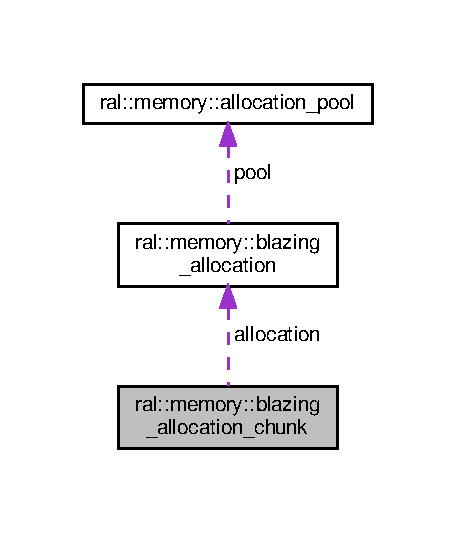
\includegraphics[width=219pt]{structral_1_1memory_1_1blazing__allocation__chunk__coll__graph}
\end{center}
\end{figure}
\subsection*{Public Attributes}
\begin{DoxyCompactItemize}
\item 
\mbox{\Hypertarget{structral_1_1memory_1_1blazing__allocation__chunk_a1c4cc63300596da92a5d17a0d2ce0420}\label{structral_1_1memory_1_1blazing__allocation__chunk_a1c4cc63300596da92a5d17a0d2ce0420}} 
std\+::size\+\_\+t {\bfseries size}
\item 
\mbox{\Hypertarget{structral_1_1memory_1_1blazing__allocation__chunk_a47417bd330d4cf9c5c86b94ebf6ba5b3}\label{structral_1_1memory_1_1blazing__allocation__chunk_a47417bd330d4cf9c5c86b94ebf6ba5b3}} 
char $\ast$ {\bfseries data}
\item 
\mbox{\Hypertarget{structral_1_1memory_1_1blazing__allocation__chunk_a6262370e4a6385ed2da015fa6787511b}\label{structral_1_1memory_1_1blazing__allocation__chunk_a6262370e4a6385ed2da015fa6787511b}} 
\hyperlink{structral_1_1memory_1_1blazing__allocation}{blazing\+\_\+allocation} $\ast$ {\bfseries allocation}
\end{DoxyCompactItemize}


The documentation for this struct was generated from the following file\+:\begin{DoxyCompactItemize}
\item 
/home/tom/\+Documents/programming/romulo\+\_\+blazingsql/blazingsql/engine/src/bmr/Buffer\+Provider.\+h\end{DoxyCompactItemize}

\hypertarget{structral_1_1memory_1_1blazing__chunked__column__info}{}\section{ral\+:\+:memory\+:\+:blazing\+\_\+chunked\+\_\+column\+\_\+info Struct Reference}
\label{structral_1_1memory_1_1blazing__chunked__column__info}\index{ral\+::memory\+::blazing\+\_\+chunked\+\_\+column\+\_\+info@{ral\+::memory\+::blazing\+\_\+chunked\+\_\+column\+\_\+info}}
\subsection*{Public Attributes}
\begin{DoxyCompactItemize}
\item 
\mbox{\Hypertarget{structral_1_1memory_1_1blazing__chunked__column__info_ade2e424a1a7c456e8603d28b3354cab0}\label{structral_1_1memory_1_1blazing__chunked__column__info_ade2e424a1a7c456e8603d28b3354cab0}} 
std\+::vector$<$ size\+\_\+t $>$ {\bfseries chunk\+\_\+index}
\item 
\mbox{\Hypertarget{structral_1_1memory_1_1blazing__chunked__column__info_a1899b994a49489806365c8bb1c3bd701}\label{structral_1_1memory_1_1blazing__chunked__column__info_a1899b994a49489806365c8bb1c3bd701}} 
std\+::vector$<$ size\+\_\+t $>$ {\bfseries offset}
\item 
\mbox{\Hypertarget{structral_1_1memory_1_1blazing__chunked__column__info_a42595677fc4a89a91b5035d6a8a33d42}\label{structral_1_1memory_1_1blazing__chunked__column__info_a42595677fc4a89a91b5035d6a8a33d42}} 
std\+::vector$<$ size\+\_\+t $>$ {\bfseries size}
\item 
\mbox{\Hypertarget{structral_1_1memory_1_1blazing__chunked__column__info_ab8efe7deb95e366b9343799ea26bd8c2}\label{structral_1_1memory_1_1blazing__chunked__column__info_ab8efe7deb95e366b9343799ea26bd8c2}} 
size\+\_\+t {\bfseries use\+\_\+size}
\end{DoxyCompactItemize}


The documentation for this struct was generated from the following file\+:\begin{DoxyCompactItemize}
\item 
/home/tom/\+Documents/programming/romulo\+\_\+blazingsql/blazingsql/engine/src/bmr/Buffer\+Provider.\+h\end{DoxyCompactItemize}

\hypertarget{classblazing__context__ref__counter}{}\section{blazing\+\_\+context\+\_\+ref\+\_\+counter Class Reference}
\label{classblazing__context__ref__counter}\index{blazing\+\_\+context\+\_\+ref\+\_\+counter@{blazing\+\_\+context\+\_\+ref\+\_\+counter}}


This class has a counter of the number of blazingcontext we have in the process.  


\subsection*{Public Member Functions}
\begin{DoxyCompactItemize}
\item 
\mbox{\Hypertarget{classblazing__context__ref__counter_a50caef06e9796fd5c94f3b8934ac638e}\label{classblazing__context__ref__counter_a50caef06e9796fd5c94f3b8934ac638e}} 
size\+\_\+t {\bfseries get\+\_\+count} () const
\item 
\mbox{\Hypertarget{classblazing__context__ref__counter_ae05c7a18707965184f735d515da42f7e}\label{classblazing__context__ref__counter_ae05c7a18707965184f735d515da42f7e}} 
void {\bfseries increase} ()
\item 
\mbox{\Hypertarget{classblazing__context__ref__counter_a54ea6fe6bb76cef1b1356d8a1b14b633}\label{classblazing__context__ref__counter_a54ea6fe6bb76cef1b1356d8a1b14b633}} 
void {\bfseries decrease} ()
\end{DoxyCompactItemize}
\subsection*{Static Public Member Functions}
\begin{DoxyCompactItemize}
\item 
\mbox{\Hypertarget{classblazing__context__ref__counter_afaa8c9b818a314d2ad8b8631052c5d51}\label{classblazing__context__ref__counter_afaa8c9b818a314d2ad8b8631052c5d51}} 
static \hyperlink{classblazing__context__ref__counter}{blazing\+\_\+context\+\_\+ref\+\_\+counter} \& {\bfseries get\+Instance} ()
\end{DoxyCompactItemize}


\subsection{Detailed Description}
This class has a counter of the number of blazingcontext we have in the process. 

The documentation for this class was generated from the following file\+:\begin{DoxyCompactItemize}
\item 
/home/tom/\+Documents/programming/romulo\+\_\+blazingsql/blazingsql/engine/src/cython/initialize.\+cpp\end{DoxyCompactItemize}

\hypertarget{classblazing__device__memory__resource}{}\section{blazing\+\_\+device\+\_\+memory\+\_\+resource Class Reference}
\label{classblazing__device__memory__resource}\index{blazing\+\_\+device\+\_\+memory\+\_\+resource@{blazing\+\_\+device\+\_\+memory\+\_\+resource}}


R\+MM \hyperlink{classblazing__device__memory__resource}{blazing\+\_\+device\+\_\+memory\+\_\+resource} class maintains the device memory manager context, including the R\+MM event log, configuration options, and registered streams.  




{\ttfamily \#include $<$Blazing\+Memory\+Resource.\+h$>$}



Inheritance diagram for blazing\+\_\+device\+\_\+memory\+\_\+resource\+:\nopagebreak
\begin{figure}[H]
\begin{center}
\leavevmode
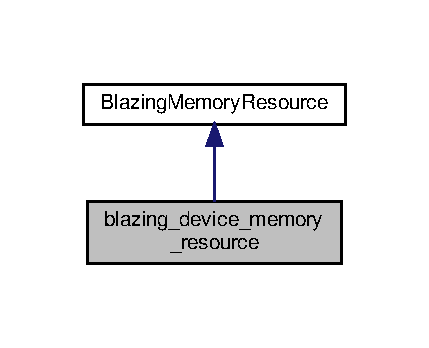
\includegraphics[width=206pt]{classblazing__device__memory__resource__inherit__graph}
\end{center}
\end{figure}


Collaboration diagram for blazing\+\_\+device\+\_\+memory\+\_\+resource\+:\nopagebreak
\begin{figure}[H]
\begin{center}
\leavevmode
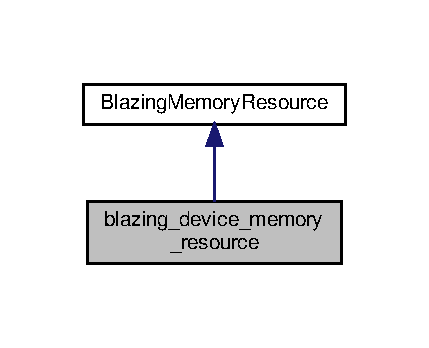
\includegraphics[width=206pt]{classblazing__device__memory__resource__coll__graph}
\end{center}
\end{figure}
\subsection*{Public Member Functions}
\begin{DoxyCompactItemize}
\item 
\mbox{\Hypertarget{classblazing__device__memory__resource_ae6a57a18e3a02583bb111a273d9b9467}\label{classblazing__device__memory__resource_ae6a57a18e3a02583bb111a273d9b9467}} 
size\+\_\+t {\bfseries get\+\_\+memory\+\_\+used} ()
\item 
\mbox{\Hypertarget{classblazing__device__memory__resource_aeacacda54cf9cc89b2f1bb30ad54a77d}\label{classblazing__device__memory__resource_aeacacda54cf9cc89b2f1bb30ad54a77d}} 
size\+\_\+t {\bfseries get\+\_\+max\+\_\+memory\+\_\+used} ()
\item 
\mbox{\Hypertarget{classblazing__device__memory__resource_a34c81aa0fe6a5d542573739a187264bb}\label{classblazing__device__memory__resource_a34c81aa0fe6a5d542573739a187264bb}} 
size\+\_\+t {\bfseries get\+\_\+total\+\_\+memory} ()
\item 
\mbox{\Hypertarget{classblazing__device__memory__resource_ac64dc046686ed83b8f6b0f85cd79517e}\label{classblazing__device__memory__resource_ac64dc046686ed83b8f6b0f85cd79517e}} 
size\+\_\+t {\bfseries get\+\_\+from\+\_\+driver\+\_\+used\+\_\+memory} ()
\item 
\mbox{\Hypertarget{classblazing__device__memory__resource_a0d0e8280d74b19fdfbab855b790c872e}\label{classblazing__device__memory__resource_a0d0e8280d74b19fdfbab855b790c872e}} 
size\+\_\+t {\bfseries get\+\_\+memory\+\_\+limit} ()
\item 
\mbox{\Hypertarget{classblazing__device__memory__resource_adcd21d872aad1620305edc061145d882}\label{classblazing__device__memory__resource_adcd21d872aad1620305edc061145d882}} 
std\+::string {\bfseries get\+\_\+type} ()
\item 
\mbox{\Hypertarget{classblazing__device__memory__resource_ac80188ecfe926a72194b98e2ad7f61e0}\label{classblazing__device__memory__resource_ac80188ecfe926a72194b98e2ad7f61e0}} 
std\+::string {\bfseries get\+\_\+full\+\_\+memory\+\_\+summary} ()
\item 
\mbox{\Hypertarget{classblazing__device__memory__resource_a3d5d3b2e31f50b773e36c5b5516144c6}\label{classblazing__device__memory__resource_a3d5d3b2e31f50b773e36c5b5516144c6}} 
void {\bfseries reset\+\_\+max\+\_\+memory\+\_\+used} (size\+\_\+t to=0)
\item 
void \hyperlink{classblazing__device__memory__resource_aff09e3f24d6448da5176747dbb37aa6b}{initialize} (std\+::string allocation\+\_\+mode, std\+::size\+\_\+t initial\+\_\+pool\+\_\+size, std\+::size\+\_\+t maximum\+\_\+pool\+\_\+size, std\+::string allocator\+\_\+logging\+\_\+file, float device\+\_\+mem\+\_\+resouce\+\_\+consumption\+\_\+thresh)
\begin{DoxyCompactList}\small\item\em Initialize R\+MM options. \end{DoxyCompactList}\item 
void \hyperlink{classblazing__device__memory__resource_ab92679fbcfe6a6075be76d3026e19b47}{finalize} ()
\item 
bool \hyperlink{classblazing__device__memory__resource_a01ae4b27062b3e30a22771edb4c625ac}{is\+Initialized} ()
\begin{DoxyCompactList}\small\item\em Check whether the \hyperlink{classblazing__device__memory__resource}{blazing\+\_\+device\+\_\+memory\+\_\+resource} has been initialized. \end{DoxyCompactList}\end{DoxyCompactItemize}
\subsection*{Static Public Member Functions}
\begin{DoxyCompactItemize}
\item 
static \hyperlink{classblazing__device__memory__resource}{blazing\+\_\+device\+\_\+memory\+\_\+resource} \& \hyperlink{classblazing__device__memory__resource_a31735d61d23aef05666c7c3f981c86fe}{get\+Instance} ()
\begin{DoxyCompactList}\small\item\em Get the \hyperlink{classblazing__device__memory__resource}{blazing\+\_\+device\+\_\+memory\+\_\+resource} instance singleton object. \end{DoxyCompactList}\end{DoxyCompactItemize}


\subsection{Detailed Description}
R\+MM \hyperlink{classblazing__device__memory__resource}{blazing\+\_\+device\+\_\+memory\+\_\+resource} class maintains the device memory manager context, including the R\+MM event log, configuration options, and registered streams. 

-\/-\/-\/-\/-\/-\/-\/-\/-\/-\/-\/-\/-\/-\/-\/-\/-\/-\/-\/-\/-\/-\/-\/-\/-\/-\/-\/-\/-\/-\/-\/-\/-\/-\/-\/-\/-\/-\/-\/-\/-\/-\/-\/-\/-\/-\/-\/-\/-\/-\/-\/-\/-\/-\/-\/-\/-\/-\/-\/-\/-\/-\/-\/-\/-\/-\/-\/-\/-\/-\/---$\ast$ \hyperlink{classblazing__device__memory__resource}{blazing\+\_\+device\+\_\+memory\+\_\+resource} is a singleton class, and should be accessed via \hyperlink{classblazing__device__memory__resource_a31735d61d23aef05666c7c3f981c86fe}{get\+Instance()}. 

\subsection{Member Function Documentation}
\mbox{\Hypertarget{classblazing__device__memory__resource_ab92679fbcfe6a6075be76d3026e19b47}\label{classblazing__device__memory__resource_ab92679fbcfe6a6075be76d3026e19b47}} 
\index{blazing\+\_\+device\+\_\+memory\+\_\+resource@{blazing\+\_\+device\+\_\+memory\+\_\+resource}!finalize@{finalize}}
\index{finalize@{finalize}!blazing\+\_\+device\+\_\+memory\+\_\+resource@{blazing\+\_\+device\+\_\+memory\+\_\+resource}}
\subsubsection{\texorpdfstring{finalize()}{finalize()}}
{\footnotesize\ttfamily void blazing\+\_\+device\+\_\+memory\+\_\+resource\+::finalize (\begin{DoxyParamCaption}{ }\end{DoxyParamCaption})}





-\/-\/-\/-\/-\/-\/-\/-\/-\/-\/-\/-\/-\/-\/-\/-\/-\/-\/-\/-\/-\/-\/-\/-\/-\/-\/-\/-\/-\/-\/-\/-\/-\/-\/-\/-\/-\/-\/-\/-\/-\/-\/-\/-\/-\/-\/-\/-\/-\/-\/-\/-\/-\/-\/-\/-\/-\/-\/-\/-\/-\/-\/-\/-\/-\/-\/-\/-\/---$\ast$ \mbox{\Hypertarget{classblazing__device__memory__resource_a31735d61d23aef05666c7c3f981c86fe}\label{classblazing__device__memory__resource_a31735d61d23aef05666c7c3f981c86fe}} 
\index{blazing\+\_\+device\+\_\+memory\+\_\+resource@{blazing\+\_\+device\+\_\+memory\+\_\+resource}!get\+Instance@{get\+Instance}}
\index{get\+Instance@{get\+Instance}!blazing\+\_\+device\+\_\+memory\+\_\+resource@{blazing\+\_\+device\+\_\+memory\+\_\+resource}}
\subsubsection{\texorpdfstring{get\+Instance()}{getInstance()}}
{\footnotesize\ttfamily static \hyperlink{classblazing__device__memory__resource}{blazing\+\_\+device\+\_\+memory\+\_\+resource}\& blazing\+\_\+device\+\_\+memory\+\_\+resource\+::get\+Instance (\begin{DoxyParamCaption}{ }\end{DoxyParamCaption})\hspace{0.3cm}{\ttfamily [inline]}, {\ttfamily [static]}}



Get the \hyperlink{classblazing__device__memory__resource}{blazing\+\_\+device\+\_\+memory\+\_\+resource} instance singleton object. 

-\/-\/-\/-\/-\/-\/-\/-\/-\/-\/-\/-\/-\/-\/-\/-\/-\/-\/-\/-\/-\/-\/-\/-\/-\/-\/-\/-\/-\/-\/-\/-\/-\/-\/-\/-\/-\/-\/-\/-\/-\/-\/-\/-\/-\/-\/-\/-\/-\/-\/-\/-\/-\/-\/-\/-\/-\/-\/-\/-\/-\/-\/-\/-\/-\/-\/-\/-\/---$\ast$ Here is the caller graph for this function\+:\nopagebreak
\begin{figure}[H]
\begin{center}
\leavevmode
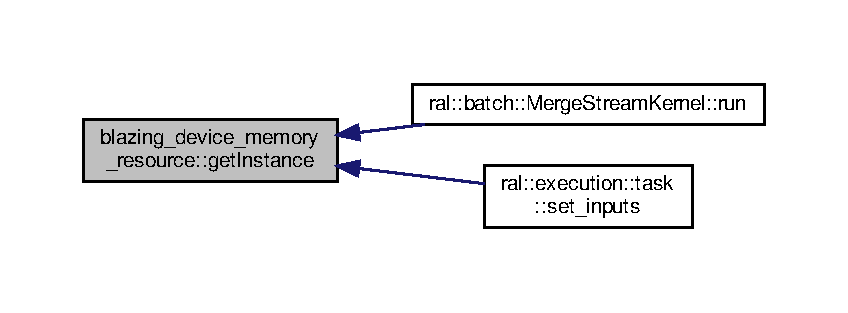
\includegraphics[width=350pt]{classblazing__device__memory__resource_a31735d61d23aef05666c7c3f981c86fe_icgraph}
\end{center}
\end{figure}
\mbox{\Hypertarget{classblazing__device__memory__resource_aff09e3f24d6448da5176747dbb37aa6b}\label{classblazing__device__memory__resource_aff09e3f24d6448da5176747dbb37aa6b}} 
\index{blazing\+\_\+device\+\_\+memory\+\_\+resource@{blazing\+\_\+device\+\_\+memory\+\_\+resource}!initialize@{initialize}}
\index{initialize@{initialize}!blazing\+\_\+device\+\_\+memory\+\_\+resource@{blazing\+\_\+device\+\_\+memory\+\_\+resource}}
\subsubsection{\texorpdfstring{initialize()}{initialize()}}
{\footnotesize\ttfamily void blazing\+\_\+device\+\_\+memory\+\_\+resource\+::initialize (\begin{DoxyParamCaption}\item[{std\+::string}]{allocation\+\_\+mode,  }\item[{std\+::size\+\_\+t}]{initial\+\_\+pool\+\_\+size,  }\item[{std\+::size\+\_\+t}]{maximum\+\_\+pool\+\_\+size,  }\item[{std\+::string}]{allocator\+\_\+logging\+\_\+file,  }\item[{float}]{device\+\_\+mem\+\_\+resouce\+\_\+consumption\+\_\+thresh }\end{DoxyParamCaption})}



Initialize R\+MM options. 

-\/-\/-\/-\/-\/-\/-\/-\/-\/-\/-\/-\/-\/-\/-\/-\/-\/-\/-\/-\/-\/-\/-\/-\/-\/-\/-\/-\/-\/-\/-\/-\/-\/-\/-\/-\/-\/-\/-\/-\/-\/-\/-\/-\/-\/-\/-\/-\/-\/-\/-\/-\/-\/-\/-\/-\/-\/-\/-\/-\/-\/-\/-\/-\/-\/-\/-\/-\/---$\ast$ allocator \+: \char`\"{}managed\char`\"{} or \char`\"{}default\char`\"{} or \char`\"{}existing\char`\"{}, where \char`\"{}managed\char`\"{} uses Unified Virtual Memory (U\+VM) and may use system memory if G\+PU memory runs out, \char`\"{}default\char`\"{} uses the default Cuda allocation and \char`\"{}existing\char`\"{} assumes rmm allocator is already set and does not initialize it. \char`\"{}managed\char`\"{} is the Blazing\+S\+QL default, since it provides the most robustness against O\+OM errors. pool \+: if True, Blazing\+Context will self-\/allocate a G\+PU memory pool. can greatly improve performance. initial\+\_\+pool\+\_\+size \+: initial size of memory pool in bytes (if pool=True). if None, and pool=True, defaults to 1/2 G\+PU memory. maximum\+\_\+pool\+\_\+size \+: maximum size of memory pool in bytes (if pool=True). if None, and pool=True, defaults to all the G\+PU memory. allocator\+\_\+logging\+\_\+file \+: File that would be used by the allocator logger. If empty, then no allocator logging will be enabled. device\+\_\+mem\+\_\+resouce\+\_\+consumption\+\_\+thresh \+: The percent (as a decimal) of total G\+PU memory that the memory resource\mbox{\Hypertarget{classblazing__device__memory__resource_a01ae4b27062b3e30a22771edb4c625ac}\label{classblazing__device__memory__resource_a01ae4b27062b3e30a22771edb4c625ac}} 
\index{blazing\+\_\+device\+\_\+memory\+\_\+resource@{blazing\+\_\+device\+\_\+memory\+\_\+resource}!is\+Initialized@{is\+Initialized}}
\index{is\+Initialized@{is\+Initialized}!blazing\+\_\+device\+\_\+memory\+\_\+resource@{blazing\+\_\+device\+\_\+memory\+\_\+resource}}
\subsubsection{\texorpdfstring{is\+Initialized()}{isInitialized()}}
{\footnotesize\ttfamily bool blazing\+\_\+device\+\_\+memory\+\_\+resource\+::is\+Initialized (\begin{DoxyParamCaption}{ }\end{DoxyParamCaption})}



Check whether the \hyperlink{classblazing__device__memory__resource}{blazing\+\_\+device\+\_\+memory\+\_\+resource} has been initialized. 

-\/-\/-\/-\/-\/-\/-\/-\/-\/-\/-\/-\/-\/-\/-\/-\/-\/-\/-\/-\/-\/-\/-\/-\/-\/-\/-\/-\/-\/-\/-\/-\/-\/-\/-\/-\/-\/-\/-\/-\/-\/-\/-\/-\/-\/-\/-\/-\/-\/-\/-\/-\/-\/-\/-\/-\/-\/-\/-\/-\/-\/-\/-\/-\/-\/-\/-\/-\/---$\ast$ \begin{DoxyReturn}{Returns}
true if \hyperlink{classblazing__device__memory__resource}{blazing\+\_\+device\+\_\+memory\+\_\+resource} has been initialized. 
\end{DoxyReturn}


The documentation for this class was generated from the following files\+:\begin{DoxyCompactItemize}
\item 
/home/tom/\+Documents/programming/romulo\+\_\+blazingsql/blazingsql/engine/src/bmr/Blazing\+Memory\+Resource.\+h\item 
/home/tom/\+Documents/programming/romulo\+\_\+blazingsql/blazingsql/engine/src/bmr/Blazing\+Memory\+Resource.\+cpp\end{DoxyCompactItemize}

\hypertarget{classblazing__disk__memory__resource}{}\section{blazing\+\_\+disk\+\_\+memory\+\_\+resource Class Reference}
\label{classblazing__disk__memory__resource}\index{blazing\+\_\+disk\+\_\+memory\+\_\+resource@{blazing\+\_\+disk\+\_\+memory\+\_\+resource}}


This class represents a custom disk memory resource used in the cache system.  




{\ttfamily \#include $<$Blazing\+Memory\+Resource.\+h$>$}



Inheritance diagram for blazing\+\_\+disk\+\_\+memory\+\_\+resource\+:\nopagebreak
\begin{figure}[H]
\begin{center}
\leavevmode
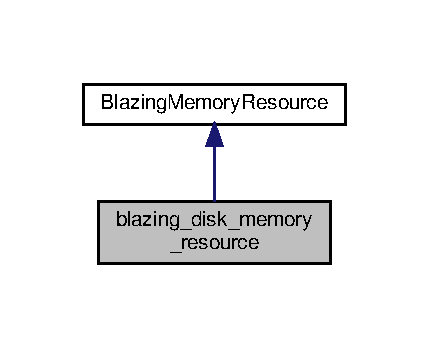
\includegraphics[width=206pt]{classblazing__disk__memory__resource__inherit__graph}
\end{center}
\end{figure}


Collaboration diagram for blazing\+\_\+disk\+\_\+memory\+\_\+resource\+:\nopagebreak
\begin{figure}[H]
\begin{center}
\leavevmode
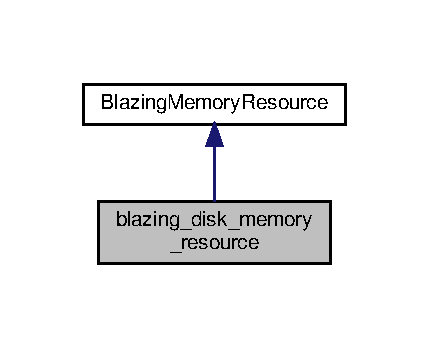
\includegraphics[width=206pt]{classblazing__disk__memory__resource__coll__graph}
\end{center}
\end{figure}
\subsection*{Public Member Functions}
\begin{DoxyCompactItemize}
\item 
\mbox{\Hypertarget{classblazing__disk__memory__resource_a67b8830405d101003182307a82f798d3}\label{classblazing__disk__memory__resource_a67b8830405d101003182307a82f798d3}} 
{\bfseries blazing\+\_\+disk\+\_\+memory\+\_\+resource} (float custom\+\_\+threshold=0.\+75)
\item 
\mbox{\Hypertarget{classblazing__disk__memory__resource_ad4651b8b5e16a09108caa6f8b681c46a}\label{classblazing__disk__memory__resource_ad4651b8b5e16a09108caa6f8b681c46a}} 
virtual size\+\_\+t {\bfseries get\+\_\+from\+\_\+driver\+\_\+used\+\_\+memory} ()
\item 
\mbox{\Hypertarget{classblazing__disk__memory__resource_ac035ec9b3f7ef86b87c7ed634ee10673}\label{classblazing__disk__memory__resource_ac035ec9b3f7ef86b87c7ed634ee10673}} 
size\+\_\+t {\bfseries get\+\_\+memory\+\_\+limit} ()
\item 
\mbox{\Hypertarget{classblazing__disk__memory__resource_a62e42fcf3251e1591c7a55f45fc5a8a0}\label{classblazing__disk__memory__resource_a62e42fcf3251e1591c7a55f45fc5a8a0}} 
size\+\_\+t {\bfseries get\+\_\+memory\+\_\+used} ()
\item 
\mbox{\Hypertarget{classblazing__disk__memory__resource_a7b38ea651ff546fd6b2c5f4dfaee14d0}\label{classblazing__disk__memory__resource_a7b38ea651ff546fd6b2c5f4dfaee14d0}} 
size\+\_\+t {\bfseries get\+\_\+total\+\_\+memory} ()
\end{DoxyCompactItemize}
\subsection*{Static Public Member Functions}
\begin{DoxyCompactItemize}
\item 
\mbox{\Hypertarget{classblazing__disk__memory__resource_ade7d366346c83c832365cca2f913d08f}\label{classblazing__disk__memory__resource_ade7d366346c83c832365cca2f913d08f}} 
static \hyperlink{classblazing__disk__memory__resource}{blazing\+\_\+disk\+\_\+memory\+\_\+resource} \& {\bfseries get\+Instance} ()
\end{DoxyCompactItemize}


\subsection{Detailed Description}
This class represents a custom disk memory resource used in the cache system. 

The documentation for this class was generated from the following files\+:\begin{DoxyCompactItemize}
\item 
/home/tom/\+Documents/programming/romulo\+\_\+blazingsql/blazingsql/engine/src/bmr/Blazing\+Memory\+Resource.\+h\item 
/home/tom/\+Documents/programming/romulo\+\_\+blazingsql/blazingsql/engine/src/bmr/Blazing\+Memory\+Resource.\+cpp\end{DoxyCompactItemize}

\hypertarget{classblazing__host__memory__resource}{}\section{blazing\+\_\+host\+\_\+memory\+\_\+resource Class Reference}
\label{classblazing__host__memory__resource}\index{blazing\+\_\+host\+\_\+memory\+\_\+resource@{blazing\+\_\+host\+\_\+memory\+\_\+resource}}


\hyperlink{classblazing__host__memory__resource}{blazing\+\_\+host\+\_\+memory\+\_\+resource} class maintains the host memory manager context.  




{\ttfamily \#include $<$Blazing\+Memory\+Resource.\+h$>$}



Inheritance diagram for blazing\+\_\+host\+\_\+memory\+\_\+resource\+:\nopagebreak
\begin{figure}[H]
\begin{center}
\leavevmode
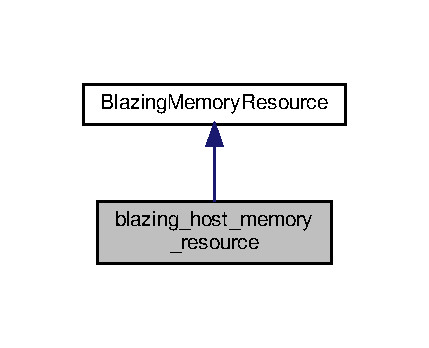
\includegraphics[width=206pt]{classblazing__host__memory__resource__inherit__graph}
\end{center}
\end{figure}


Collaboration diagram for blazing\+\_\+host\+\_\+memory\+\_\+resource\+:\nopagebreak
\begin{figure}[H]
\begin{center}
\leavevmode
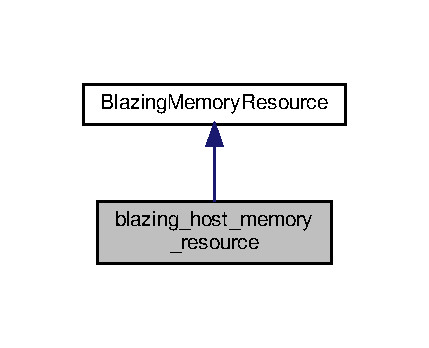
\includegraphics[width=206pt]{classblazing__host__memory__resource__coll__graph}
\end{center}
\end{figure}
\subsection*{Public Member Functions}
\begin{DoxyCompactItemize}
\item 
\mbox{\Hypertarget{classblazing__host__memory__resource_a3ada1edd4d72ed90b5b545e83590fcb1}\label{classblazing__host__memory__resource_a3ada1edd4d72ed90b5b545e83590fcb1}} 
size\+\_\+t {\bfseries get\+\_\+memory\+\_\+used} () override
\item 
\mbox{\Hypertarget{classblazing__host__memory__resource_aaf5b08aae1b6d60fdf30c1b4cb0b0ed2}\label{classblazing__host__memory__resource_aaf5b08aae1b6d60fdf30c1b4cb0b0ed2}} 
size\+\_\+t {\bfseries get\+\_\+total\+\_\+memory} () override
\item 
\mbox{\Hypertarget{classblazing__host__memory__resource_a15c8bcb4ef3618d82a18bf8dd3909ef5}\label{classblazing__host__memory__resource_a15c8bcb4ef3618d82a18bf8dd3909ef5}} 
size\+\_\+t {\bfseries get\+\_\+from\+\_\+driver\+\_\+used\+\_\+memory} ()
\item 
\mbox{\Hypertarget{classblazing__host__memory__resource_a91cb1fe1caf14c6fd2c42a12cc51e116}\label{classblazing__host__memory__resource_a91cb1fe1caf14c6fd2c42a12cc51e116}} 
size\+\_\+t {\bfseries get\+\_\+memory\+\_\+limit} ()
\item 
\mbox{\Hypertarget{classblazing__host__memory__resource_aae6e1f9fe638d2bd4924451656d0a3dd}\label{classblazing__host__memory__resource_aae6e1f9fe638d2bd4924451656d0a3dd}} 
void {\bfseries allocate} (std\+::size\+\_\+t bytes)
\item 
\mbox{\Hypertarget{classblazing__host__memory__resource_aaab7cf28a013ae371d4c5850041679b5}\label{classblazing__host__memory__resource_aaab7cf28a013ae371d4c5850041679b5}} 
void {\bfseries deallocate} (std\+::size\+\_\+t bytes)
\item 
void \hyperlink{classblazing__host__memory__resource_a24f72f410d6ef29937661e2fe79fd292}{initialize} (float host\+\_\+mem\+\_\+resouce\+\_\+consumption\+\_\+thresh)
\begin{DoxyCompactList}\small\item\em Initialize. \end{DoxyCompactList}\item 
void \hyperlink{classblazing__host__memory__resource_a05d933cea38920323a6d9d006019fac3}{finalize} ()
\item 
bool \hyperlink{classblazing__host__memory__resource_a863f02392dbfc839f87b8b3a2a6cff9e}{is\+Initialized} ()
\begin{DoxyCompactList}\small\item\em Check whether the \hyperlink{classblazing__device__memory__resource}{blazing\+\_\+device\+\_\+memory\+\_\+resource} has been initialized. \end{DoxyCompactList}\end{DoxyCompactItemize}
\subsection*{Static Public Member Functions}
\begin{DoxyCompactItemize}
\item 
static \hyperlink{classblazing__host__memory__resource}{blazing\+\_\+host\+\_\+memory\+\_\+resource} \& \hyperlink{classblazing__host__memory__resource_a1fa50b80350c0718dc4ee026e8425e7a}{get\+Instance} ()
\begin{DoxyCompactList}\small\item\em Get the \hyperlink{classblazing__host__memory__resource}{blazing\+\_\+host\+\_\+memory\+\_\+resource} instance singleton object. \end{DoxyCompactList}\end{DoxyCompactItemize}


\subsection{Detailed Description}
\hyperlink{classblazing__host__memory__resource}{blazing\+\_\+host\+\_\+memory\+\_\+resource} class maintains the host memory manager context. 

-\/-\/-\/-\/-\/-\/-\/-\/-\/-\/-\/-\/-\/-\/-\/-\/-\/-\/-\/-\/-\/-\/-\/-\/-\/-\/-\/-\/-\/-\/-\/-\/-\/-\/-\/-\/-\/-\/-\/-\/-\/-\/-\/-\/-\/-\/-\/-\/-\/-\/-\/-\/-\/-\/-\/-\/-\/-\/-\/-\/-\/-\/-\/-\/-\/-\/-\/-\/-\/-\/---$\ast$ \hyperlink{classblazing__host__memory__resource}{blazing\+\_\+host\+\_\+memory\+\_\+resource} is a singleton class, and should be accessed via \hyperlink{classblazing__host__memory__resource_a1fa50b80350c0718dc4ee026e8425e7a}{get\+Instance()}. 

\subsection{Member Function Documentation}
\mbox{\Hypertarget{classblazing__host__memory__resource_a05d933cea38920323a6d9d006019fac3}\label{classblazing__host__memory__resource_a05d933cea38920323a6d9d006019fac3}} 
\index{blazing\+\_\+host\+\_\+memory\+\_\+resource@{blazing\+\_\+host\+\_\+memory\+\_\+resource}!finalize@{finalize}}
\index{finalize@{finalize}!blazing\+\_\+host\+\_\+memory\+\_\+resource@{blazing\+\_\+host\+\_\+memory\+\_\+resource}}
\subsubsection{\texorpdfstring{finalize()}{finalize()}}
{\footnotesize\ttfamily void blazing\+\_\+host\+\_\+memory\+\_\+resource\+::finalize (\begin{DoxyParamCaption}{ }\end{DoxyParamCaption})}





-\/-\/-\/-\/-\/-\/-\/-\/-\/-\/-\/-\/-\/-\/-\/-\/-\/-\/-\/-\/-\/-\/-\/-\/-\/-\/-\/-\/-\/-\/-\/-\/-\/-\/-\/-\/-\/-\/-\/-\/-\/-\/-\/-\/-\/-\/-\/-\/-\/-\/-\/-\/-\/-\/-\/-\/-\/-\/-\/-\/-\/-\/-\/-\/-\/-\/-\/-\/---$\ast$ \mbox{\Hypertarget{classblazing__host__memory__resource_a1fa50b80350c0718dc4ee026e8425e7a}\label{classblazing__host__memory__resource_a1fa50b80350c0718dc4ee026e8425e7a}} 
\index{blazing\+\_\+host\+\_\+memory\+\_\+resource@{blazing\+\_\+host\+\_\+memory\+\_\+resource}!get\+Instance@{get\+Instance}}
\index{get\+Instance@{get\+Instance}!blazing\+\_\+host\+\_\+memory\+\_\+resource@{blazing\+\_\+host\+\_\+memory\+\_\+resource}}
\subsubsection{\texorpdfstring{get\+Instance()}{getInstance()}}
{\footnotesize\ttfamily static \hyperlink{classblazing__host__memory__resource}{blazing\+\_\+host\+\_\+memory\+\_\+resource}\& blazing\+\_\+host\+\_\+memory\+\_\+resource\+::get\+Instance (\begin{DoxyParamCaption}{ }\end{DoxyParamCaption})\hspace{0.3cm}{\ttfamily [inline]}, {\ttfamily [static]}}



Get the \hyperlink{classblazing__host__memory__resource}{blazing\+\_\+host\+\_\+memory\+\_\+resource} instance singleton object. 

-\/-\/-\/-\/-\/-\/-\/-\/-\/-\/-\/-\/-\/-\/-\/-\/-\/-\/-\/-\/-\/-\/-\/-\/-\/-\/-\/-\/-\/-\/-\/-\/-\/-\/-\/-\/-\/-\/-\/-\/-\/-\/-\/-\/-\/-\/-\/-\/-\/-\/-\/-\/-\/-\/-\/-\/-\/-\/-\/-\/-\/-\/-\/-\/-\/-\/-\/-\/---$\ast$ \mbox{\Hypertarget{classblazing__host__memory__resource_a24f72f410d6ef29937661e2fe79fd292}\label{classblazing__host__memory__resource_a24f72f410d6ef29937661e2fe79fd292}} 
\index{blazing\+\_\+host\+\_\+memory\+\_\+resource@{blazing\+\_\+host\+\_\+memory\+\_\+resource}!initialize@{initialize}}
\index{initialize@{initialize}!blazing\+\_\+host\+\_\+memory\+\_\+resource@{blazing\+\_\+host\+\_\+memory\+\_\+resource}}
\subsubsection{\texorpdfstring{initialize()}{initialize()}}
{\footnotesize\ttfamily void blazing\+\_\+host\+\_\+memory\+\_\+resource\+::initialize (\begin{DoxyParamCaption}\item[{float}]{host\+\_\+mem\+\_\+resouce\+\_\+consumption\+\_\+thresh }\end{DoxyParamCaption})}



Initialize. 

-\/-\/-\/-\/-\/-\/-\/-\/-\/-\/-\/-\/-\/-\/-\/-\/-\/-\/-\/-\/-\/-\/-\/-\/-\/-\/-\/-\/-\/-\/-\/-\/-\/-\/-\/-\/-\/-\/-\/-\/-\/-\/-\/-\/-\/-\/-\/-\/-\/-\/-\/-\/-\/-\/-\/-\/-\/-\/-\/-\/-\/-\/-\/-\/-\/-\/-\/-\/---$\ast$ Accepts an optional rmm\+Options\+\_\+t struct that describes the settings used to initialize the memory manager. If no {\ttfamily options} is passed, default options are used.\mbox{\Hypertarget{classblazing__host__memory__resource_a863f02392dbfc839f87b8b3a2a6cff9e}\label{classblazing__host__memory__resource_a863f02392dbfc839f87b8b3a2a6cff9e}} 
\index{blazing\+\_\+host\+\_\+memory\+\_\+resource@{blazing\+\_\+host\+\_\+memory\+\_\+resource}!is\+Initialized@{is\+Initialized}}
\index{is\+Initialized@{is\+Initialized}!blazing\+\_\+host\+\_\+memory\+\_\+resource@{blazing\+\_\+host\+\_\+memory\+\_\+resource}}
\subsubsection{\texorpdfstring{is\+Initialized()}{isInitialized()}}
{\footnotesize\ttfamily bool blazing\+\_\+host\+\_\+memory\+\_\+resource\+::is\+Initialized (\begin{DoxyParamCaption}{ }\end{DoxyParamCaption})}



Check whether the \hyperlink{classblazing__device__memory__resource}{blazing\+\_\+device\+\_\+memory\+\_\+resource} has been initialized. 

-\/-\/-\/-\/-\/-\/-\/-\/-\/-\/-\/-\/-\/-\/-\/-\/-\/-\/-\/-\/-\/-\/-\/-\/-\/-\/-\/-\/-\/-\/-\/-\/-\/-\/-\/-\/-\/-\/-\/-\/-\/-\/-\/-\/-\/-\/-\/-\/-\/-\/-\/-\/-\/-\/-\/-\/-\/-\/-\/-\/-\/-\/-\/-\/-\/-\/-\/-\/---$\ast$ \begin{DoxyReturn}{Returns}
true if \hyperlink{classblazing__device__memory__resource}{blazing\+\_\+device\+\_\+memory\+\_\+resource} has been initialized. 
\end{DoxyReturn}


The documentation for this class was generated from the following files\+:\begin{DoxyCompactItemize}
\item 
/home/tom/\+Documents/programming/romulo\+\_\+blazingsql/blazingsql/engine/src/bmr/Blazing\+Memory\+Resource.\+h\item 
/home/tom/\+Documents/programming/romulo\+\_\+blazingsql/blazingsql/engine/src/bmr/Blazing\+Memory\+Resource.\+cpp\end{DoxyCompactItemize}

\hypertarget{structcomm_1_1blazing__ucp__tag}{}\section{comm\+:\+:blazing\+\_\+ucp\+\_\+tag Struct Reference}
\label{structcomm_1_1blazing__ucp__tag}\index{comm\+::blazing\+\_\+ucp\+\_\+tag@{comm\+::blazing\+\_\+ucp\+\_\+tag}}


{\ttfamily \#include $<$message\+Receiver.\+hpp$>$}

\subsection*{Public Attributes}
\begin{DoxyCompactItemize}
\item 
int \hyperlink{structcomm_1_1blazing__ucp__tag_a31f59e8f5c2a690df88ca3a4147ef942}{message\+\_\+id}
\item 
uint16\+\_\+t \hyperlink{structcomm_1_1blazing__ucp__tag_ae34c2b757572ae3316c4c52b220e368b}{worker\+\_\+origin\+\_\+id}
\item 
uint16\+\_\+t \hyperlink{structcomm_1_1blazing__ucp__tag_ae5f3239906e71a91821ae27d4ec17325}{frame\+\_\+id}
\end{DoxyCompactItemize}


\subsection{Detailed Description}
A struct for managing the 64 bit tag that ucx uses This allow us to make a value that is stored in 8 bytes 

\subsection{Member Data Documentation}
\mbox{\Hypertarget{structcomm_1_1blazing__ucp__tag_ae5f3239906e71a91821ae27d4ec17325}\label{structcomm_1_1blazing__ucp__tag_ae5f3239906e71a91821ae27d4ec17325}} 
\index{comm\+::blazing\+\_\+ucp\+\_\+tag@{comm\+::blazing\+\_\+ucp\+\_\+tag}!frame\+\_\+id@{frame\+\_\+id}}
\index{frame\+\_\+id@{frame\+\_\+id}!comm\+::blazing\+\_\+ucp\+\_\+tag@{comm\+::blazing\+\_\+ucp\+\_\+tag}}
\subsubsection{\texorpdfstring{frame\+\_\+id}{frame\_id}}
{\footnotesize\ttfamily uint16\+\_\+t comm\+::blazing\+\_\+ucp\+\_\+tag\+::frame\+\_\+id}

The id of the frame being sent. 0 for being\+\_\+transmission \mbox{\Hypertarget{structcomm_1_1blazing__ucp__tag_a31f59e8f5c2a690df88ca3a4147ef942}\label{structcomm_1_1blazing__ucp__tag_a31f59e8f5c2a690df88ca3a4147ef942}} 
\index{comm\+::blazing\+\_\+ucp\+\_\+tag@{comm\+::blazing\+\_\+ucp\+\_\+tag}!message\+\_\+id@{message\+\_\+id}}
\index{message\+\_\+id@{message\+\_\+id}!comm\+::blazing\+\_\+ucp\+\_\+tag@{comm\+::blazing\+\_\+ucp\+\_\+tag}}
\subsubsection{\texorpdfstring{message\+\_\+id}{message\_id}}
{\footnotesize\ttfamily int comm\+::blazing\+\_\+ucp\+\_\+tag\+::message\+\_\+id}

The message id which is generated by a global atomic \mbox{\Hypertarget{structcomm_1_1blazing__ucp__tag_ae34c2b757572ae3316c4c52b220e368b}\label{structcomm_1_1blazing__ucp__tag_ae34c2b757572ae3316c4c52b220e368b}} 
\index{comm\+::blazing\+\_\+ucp\+\_\+tag@{comm\+::blazing\+\_\+ucp\+\_\+tag}!worker\+\_\+origin\+\_\+id@{worker\+\_\+origin\+\_\+id}}
\index{worker\+\_\+origin\+\_\+id@{worker\+\_\+origin\+\_\+id}!comm\+::blazing\+\_\+ucp\+\_\+tag@{comm\+::blazing\+\_\+ucp\+\_\+tag}}
\subsubsection{\texorpdfstring{worker\+\_\+origin\+\_\+id}{worker\_origin\_id}}
{\footnotesize\ttfamily uint16\+\_\+t comm\+::blazing\+\_\+ucp\+\_\+tag\+::worker\+\_\+origin\+\_\+id}

The id to make sure each tag is unique 

The documentation for this struct was generated from the following file\+:\begin{DoxyCompactItemize}
\item 
/home/tom/\+Documents/programming/romulo\+\_\+blazingsql/blazingsql/engine/src/communication/\+Communication\+Interface/message\+Receiver.\+hpp\end{DoxyCompactItemize}

\hypertarget{classral_1_1frame_1_1BlazingColumn}{}\section{ral\+:\+:frame\+:\+:Blazing\+Column Class Reference}
\label{classral_1_1frame_1_1BlazingColumn}\index{ral\+::frame\+::\+Blazing\+Column@{ral\+::frame\+::\+Blazing\+Column}}


Inheritance diagram for ral\+:\+:frame\+:\+:Blazing\+Column\+:\nopagebreak
\begin{figure}[H]
\begin{center}
\leavevmode
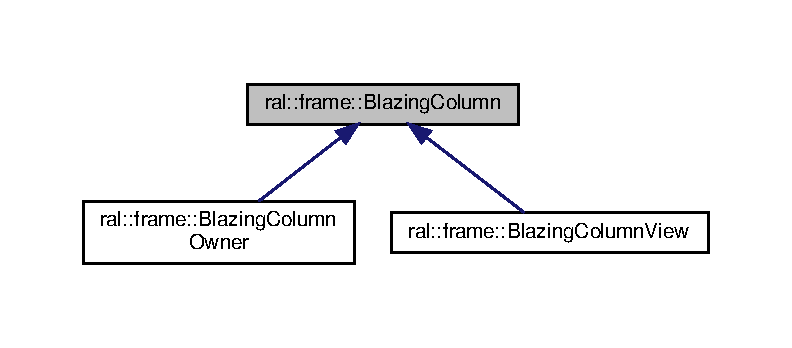
\includegraphics[width=350pt]{classral_1_1frame_1_1BlazingColumn__inherit__graph}
\end{center}
\end{figure}
\subsection*{Public Member Functions}
\begin{DoxyCompactItemize}
\item 
\mbox{\Hypertarget{classral_1_1frame_1_1BlazingColumn_aa925ea5a4e2c3577b938cfbe840abd62}\label{classral_1_1frame_1_1BlazingColumn_aa925ea5a4e2c3577b938cfbe840abd62}} 
{\bfseries Blazing\+Column} (const \hyperlink{classral_1_1frame_1_1BlazingColumn}{Blazing\+Column} \&)=delete
\item 
\mbox{\Hypertarget{classral_1_1frame_1_1BlazingColumn_aec09cbf7352b0a51ef81bdcd34fd409a}\label{classral_1_1frame_1_1BlazingColumn_aec09cbf7352b0a51ef81bdcd34fd409a}} 
\hyperlink{classral_1_1frame_1_1BlazingColumn}{Blazing\+Column} \& {\bfseries operator=} (const \hyperlink{classral_1_1frame_1_1BlazingColumn}{Blazing\+Column} \&)=delete
\item 
\mbox{\Hypertarget{classral_1_1frame_1_1BlazingColumn_ad2552e447b9761a982a6bd11a3882243}\label{classral_1_1frame_1_1BlazingColumn_ad2552e447b9761a982a6bd11a3882243}} 
virtual Cudf\+Column\+View {\bfseries view} () const =0
\item 
\mbox{\Hypertarget{classral_1_1frame_1_1BlazingColumn_a479d643c8e684bcb5583d289b38f8e8c}\label{classral_1_1frame_1_1BlazingColumn_a479d643c8e684bcb5583d289b38f8e8c}} 
virtual std\+::unique\+\_\+ptr$<$ Cudf\+Column $>$ {\bfseries release} ()=0
\item 
\mbox{\Hypertarget{classral_1_1frame_1_1BlazingColumn_ad75eccd073f4af1bf312b9f667b252d8}\label{classral_1_1frame_1_1BlazingColumn_ad75eccd073f4af1bf312b9f667b252d8}} 
virtual blazing\+\_\+column\+\_\+type {\bfseries type} ()=0
\end{DoxyCompactItemize}


The documentation for this class was generated from the following file\+:\begin{DoxyCompactItemize}
\item 
/home/tom/\+Documents/programming/romulo\+\_\+blazingsql/blazingsql/engine/src/execution\+\_\+graph/logic\+\_\+controllers/Blazing\+Column.\+h\end{DoxyCompactItemize}

\hypertarget{classral_1_1frame_1_1BlazingColumnOwner}{}\section{ral\+:\+:frame\+:\+:Blazing\+Column\+Owner Class Reference}
\label{classral_1_1frame_1_1BlazingColumnOwner}\index{ral\+::frame\+::\+Blazing\+Column\+Owner@{ral\+::frame\+::\+Blazing\+Column\+Owner}}


Inheritance diagram for ral\+:\+:frame\+:\+:Blazing\+Column\+Owner\+:\nopagebreak
\begin{figure}[H]
\begin{center}
\leavevmode
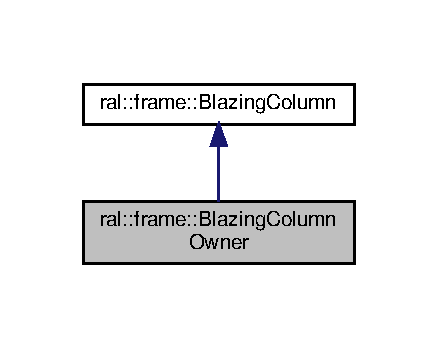
\includegraphics[width=210pt]{classral_1_1frame_1_1BlazingColumnOwner__inherit__graph}
\end{center}
\end{figure}


Collaboration diagram for ral\+:\+:frame\+:\+:Blazing\+Column\+Owner\+:\nopagebreak
\begin{figure}[H]
\begin{center}
\leavevmode
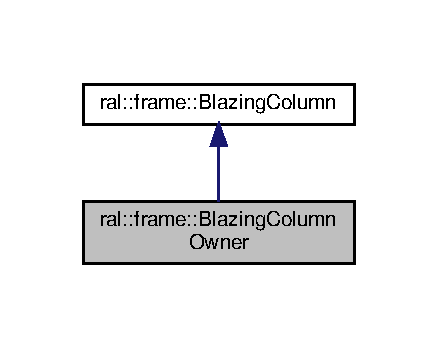
\includegraphics[width=210pt]{classral_1_1frame_1_1BlazingColumnOwner__coll__graph}
\end{center}
\end{figure}
\subsection*{Public Member Functions}
\begin{DoxyCompactItemize}
\item 
\mbox{\Hypertarget{classral_1_1frame_1_1BlazingColumnOwner_a917c09bd16079fc64a19f5b8e68a4c00}\label{classral_1_1frame_1_1BlazingColumnOwner_a917c09bd16079fc64a19f5b8e68a4c00}} 
{\bfseries Blazing\+Column\+Owner} (const \hyperlink{classral_1_1frame_1_1BlazingColumn}{Blazing\+Column} \&)=delete
\item 
\mbox{\Hypertarget{classral_1_1frame_1_1BlazingColumnOwner_a6d49038ec53dc7a35fec3727d91852fa}\label{classral_1_1frame_1_1BlazingColumnOwner_a6d49038ec53dc7a35fec3727d91852fa}} 
\hyperlink{classral_1_1frame_1_1BlazingColumnOwner}{Blazing\+Column\+Owner} \& {\bfseries operator=} (const \hyperlink{classral_1_1frame_1_1BlazingColumnOwner}{Blazing\+Column\+Owner} \&)=delete
\item 
\mbox{\Hypertarget{classral_1_1frame_1_1BlazingColumnOwner_a435fa4fe80fd584647f3381ca578db88}\label{classral_1_1frame_1_1BlazingColumnOwner_a435fa4fe80fd584647f3381ca578db88}} 
{\bfseries Blazing\+Column\+Owner} (std\+::unique\+\_\+ptr$<$ Cudf\+Column $>$ column)
\item 
\mbox{\Hypertarget{classral_1_1frame_1_1BlazingColumnOwner_ae9fc48497fb4ef45777d66c6888311f6}\label{classral_1_1frame_1_1BlazingColumnOwner_ae9fc48497fb4ef45777d66c6888311f6}} 
Cudf\+Column\+View {\bfseries view} () const
\item 
\mbox{\Hypertarget{classral_1_1frame_1_1BlazingColumnOwner_aa103e63483906f95a701d83bbb94fd82}\label{classral_1_1frame_1_1BlazingColumnOwner_aa103e63483906f95a701d83bbb94fd82}} 
std\+::unique\+\_\+ptr$<$ Cudf\+Column $>$ {\bfseries release} ()
\item 
\mbox{\Hypertarget{classral_1_1frame_1_1BlazingColumnOwner_a9fa77ce1e4bff77a021b623e5f891833}\label{classral_1_1frame_1_1BlazingColumnOwner_a9fa77ce1e4bff77a021b623e5f891833}} 
blazing\+\_\+column\+\_\+type {\bfseries type} ()
\end{DoxyCompactItemize}


The documentation for this class was generated from the following files\+:\begin{DoxyCompactItemize}
\item 
/home/tom/\+Documents/programming/romulo\+\_\+blazingsql/blazingsql/engine/src/execution\+\_\+graph/logic\+\_\+controllers/Blazing\+Column\+Owner.\+h\item 
/home/tom/\+Documents/programming/romulo\+\_\+blazingsql/blazingsql/engine/src/execution\+\_\+graph/logic\+\_\+controllers/Blazing\+Column\+Owner.\+cpp\end{DoxyCompactItemize}

\hypertarget{classral_1_1frame_1_1BlazingColumnView}{}\section{ral\+:\+:frame\+:\+:Blazing\+Column\+View Class Reference}
\label{classral_1_1frame_1_1BlazingColumnView}\index{ral\+::frame\+::\+Blazing\+Column\+View@{ral\+::frame\+::\+Blazing\+Column\+View}}


Inheritance diagram for ral\+:\+:frame\+:\+:Blazing\+Column\+View\+:\nopagebreak
\begin{figure}[H]
\begin{center}
\leavevmode
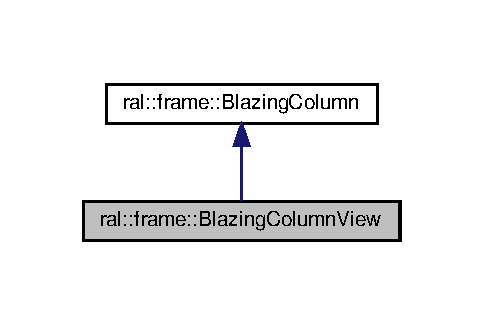
\includegraphics[width=232pt]{classral_1_1frame_1_1BlazingColumnView__inherit__graph}
\end{center}
\end{figure}


Collaboration diagram for ral\+:\+:frame\+:\+:Blazing\+Column\+View\+:\nopagebreak
\begin{figure}[H]
\begin{center}
\leavevmode
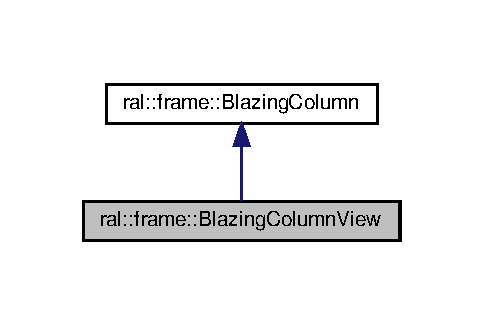
\includegraphics[width=232pt]{classral_1_1frame_1_1BlazingColumnView__coll__graph}
\end{center}
\end{figure}
\subsection*{Public Member Functions}
\begin{DoxyCompactItemize}
\item 
\mbox{\Hypertarget{classral_1_1frame_1_1BlazingColumnView_a6614bc3303e9ddae2ca82b5f683db1e5}\label{classral_1_1frame_1_1BlazingColumnView_a6614bc3303e9ddae2ca82b5f683db1e5}} 
{\bfseries Blazing\+Column\+View} (const \hyperlink{classral_1_1frame_1_1BlazingColumn}{Blazing\+Column} \&)=delete
\item 
\mbox{\Hypertarget{classral_1_1frame_1_1BlazingColumnView_ac1364ad89ec54cbbc9519586e8c79025}\label{classral_1_1frame_1_1BlazingColumnView_ac1364ad89ec54cbbc9519586e8c79025}} 
\hyperlink{classral_1_1frame_1_1BlazingColumnView}{Blazing\+Column\+View} \& {\bfseries operator=} (const \hyperlink{classral_1_1frame_1_1BlazingColumnView}{Blazing\+Column\+View} \&)=delete
\item 
\mbox{\Hypertarget{classral_1_1frame_1_1BlazingColumnView_aaf2c734c09c9598cb033fb16e75b6084}\label{classral_1_1frame_1_1BlazingColumnView_aaf2c734c09c9598cb033fb16e75b6084}} 
{\bfseries Blazing\+Column\+View} (const Cudf\+Column\+View \&column)
\item 
\mbox{\Hypertarget{classral_1_1frame_1_1BlazingColumnView_ae4efd39e2da5a7b12ddc757e75612f57}\label{classral_1_1frame_1_1BlazingColumnView_ae4efd39e2da5a7b12ddc757e75612f57}} 
Cudf\+Column\+View {\bfseries view} () const
\item 
\mbox{\Hypertarget{classral_1_1frame_1_1BlazingColumnView_ae6777c3e3e891ba83211a3313da79564}\label{classral_1_1frame_1_1BlazingColumnView_ae6777c3e3e891ba83211a3313da79564}} 
std\+::unique\+\_\+ptr$<$ Cudf\+Column $>$ {\bfseries release} ()
\item 
\mbox{\Hypertarget{classral_1_1frame_1_1BlazingColumnView_a15b97df0965af74f65b4f896b97ae980}\label{classral_1_1frame_1_1BlazingColumnView_a15b97df0965af74f65b4f896b97ae980}} 
blazing\+\_\+column\+\_\+type {\bfseries type} ()
\end{DoxyCompactItemize}


The documentation for this class was generated from the following file\+:\begin{DoxyCompactItemize}
\item 
/home/tom/\+Documents/programming/romulo\+\_\+blazingsql/blazingsql/engine/src/execution\+\_\+graph/logic\+\_\+controllers/Blazing\+Column\+View.\+h\end{DoxyCompactItemize}

\hypertarget{classral_1_1frame_1_1BlazingHostTable}{}\section{ral\+:\+:frame\+:\+:Blazing\+Host\+Table Class Reference}
\label{classral_1_1frame_1_1BlazingHostTable}\index{ral\+::frame\+::\+Blazing\+Host\+Table@{ral\+::frame\+::\+Blazing\+Host\+Table}}


A class that represents the \hyperlink{classral_1_1frame_1_1BlazingTable}{Blazing\+Table} store in host memory. This implementation uses only raw allocations, Column\+Transports and chunked\+\_\+column\+\_\+infos that represent a \hyperlink{classral_1_1frame_1_1BlazingTable}{Blazing\+Table}. The reference to implement this class was based on the way how \hyperlink{classral_1_1frame_1_1BlazingTable}{Blazing\+Table} objects are send/received by the communication library.  




{\ttfamily \#include $<$Blazing\+Host\+Table.\+h$>$}

\subsection*{Public Member Functions}
\begin{DoxyCompactItemize}
\item 
\mbox{\Hypertarget{classral_1_1frame_1_1BlazingHostTable_ad61570c773d3d83c788d1a66ef657b1f}\label{classral_1_1frame_1_1BlazingHostTable_ad61570c773d3d83c788d1a66ef657b1f}} 
{\bfseries Blazing\+Host\+Table} (const std\+::vector$<$ \hyperlink{structblazingdb_1_1transport_1_1ColumnTransport}{Column\+Transport} $>$ \&columns\+\_\+offsets, std\+::vector$<$ \hyperlink{structral_1_1memory_1_1blazing__chunked__column__info}{ral\+::memory\+::blazing\+\_\+chunked\+\_\+column\+\_\+info} $>$ \&\&chunked\+\_\+column\+\_\+infos, std\+::vector$<$ std\+::unique\+\_\+ptr$<$ \hyperlink{structral_1_1memory_1_1blazing__allocation__chunk}{ral\+::memory\+::blazing\+\_\+allocation\+\_\+chunk} $>$$>$ \&\&allocations)
\item 
\mbox{\Hypertarget{classral_1_1frame_1_1BlazingHostTable_a81bf7375e4c76c00615a141243edd891}\label{classral_1_1frame_1_1BlazingHostTable_a81bf7375e4c76c00615a141243edd891}} 
std\+::vector$<$ cudf\+::data\+\_\+type $>$ {\bfseries get\+\_\+schema} () const
\item 
\mbox{\Hypertarget{classral_1_1frame_1_1BlazingHostTable_afc36b1cebafd2be252e1fe86f358c047}\label{classral_1_1frame_1_1BlazingHostTable_afc36b1cebafd2be252e1fe86f358c047}} 
std\+::vector$<$ std\+::string $>$ {\bfseries names} () const
\item 
\mbox{\Hypertarget{classral_1_1frame_1_1BlazingHostTable_ad48051c54ff7a7bce9261fcd58f1815c}\label{classral_1_1frame_1_1BlazingHostTable_ad48051c54ff7a7bce9261fcd58f1815c}} 
void {\bfseries set\+\_\+names} (std\+::vector$<$ std\+::string $>$ names)
\item 
\mbox{\Hypertarget{classral_1_1frame_1_1BlazingHostTable_a8c79df309ba2224a497e3ff26d22c399}\label{classral_1_1frame_1_1BlazingHostTable_a8c79df309ba2224a497e3ff26d22c399}} 
cudf\+::size\+\_\+type {\bfseries num\+\_\+rows} () const
\item 
\mbox{\Hypertarget{classral_1_1frame_1_1BlazingHostTable_a7d1f2bc7f684b2494f54af56fac94555}\label{classral_1_1frame_1_1BlazingHostTable_a7d1f2bc7f684b2494f54af56fac94555}} 
cudf\+::size\+\_\+type {\bfseries num\+\_\+columns} () const
\item 
\mbox{\Hypertarget{classral_1_1frame_1_1BlazingHostTable_a55117c800b864710d6ebcc72cfec23fc}\label{classral_1_1frame_1_1BlazingHostTable_a55117c800b864710d6ebcc72cfec23fc}} 
std\+::size\+\_\+t {\bfseries size\+In\+Bytes} ()
\item 
\mbox{\Hypertarget{classral_1_1frame_1_1BlazingHostTable_ad919bd6ff9ebd4601fe0171d9b1c4ca1}\label{classral_1_1frame_1_1BlazingHostTable_ad919bd6ff9ebd4601fe0171d9b1c4ca1}} 
void {\bfseries set\+Partition\+Id} (const size\+\_\+t \&part\+\_\+id)
\item 
\mbox{\Hypertarget{classral_1_1frame_1_1BlazingHostTable_a5d5a24d3d43fc074264a88e66d544ffa}\label{classral_1_1frame_1_1BlazingHostTable_a5d5a24d3d43fc074264a88e66d544ffa}} 
size\+\_\+t {\bfseries get\+\_\+part\+\_\+id} ()
\item 
\mbox{\Hypertarget{classral_1_1frame_1_1BlazingHostTable_a3e510befe328cce2016555fe4f6c32bc}\label{classral_1_1frame_1_1BlazingHostTable_a3e510befe328cce2016555fe4f6c32bc}} 
const std\+::vector$<$ \hyperlink{structblazingdb_1_1transport_1_1ColumnTransport}{Column\+Transport} $>$ \& {\bfseries get\+\_\+columns\+\_\+offsets} () const
\item 
\mbox{\Hypertarget{classral_1_1frame_1_1BlazingHostTable_afc324a9367a9bd0bea7a171c782e91d2}\label{classral_1_1frame_1_1BlazingHostTable_afc324a9367a9bd0bea7a171c782e91d2}} 
std\+::unique\+\_\+ptr$<$ \hyperlink{classral_1_1frame_1_1BlazingTable}{Blazing\+Table} $>$ {\bfseries get\+\_\+gpu\+\_\+table} () const
\item 
\mbox{\Hypertarget{classral_1_1frame_1_1BlazingHostTable_a916b3247a17306ad2a53ea032f03407a}\label{classral_1_1frame_1_1BlazingHostTable_a916b3247a17306ad2a53ea032f03407a}} 
std\+::vector$<$ \hyperlink{structral_1_1memory_1_1blazing__allocation__chunk}{ral\+::memory\+::blazing\+\_\+allocation\+\_\+chunk} $>$ {\bfseries get\+\_\+raw\+\_\+buffers} () const
\item 
\mbox{\Hypertarget{classral_1_1frame_1_1BlazingHostTable_a6c8bd9f79e0f7eb27ae007a4acf8a9b4}\label{classral_1_1frame_1_1BlazingHostTable_a6c8bd9f79e0f7eb27ae007a4acf8a9b4}} 
const std\+::vector$<$ \hyperlink{structral_1_1memory_1_1blazing__chunked__column__info}{ral\+::memory\+::blazing\+\_\+chunked\+\_\+column\+\_\+info} $>$ \& {\bfseries get\+\_\+blazing\+\_\+chunked\+\_\+column\+\_\+infos} () const
\end{DoxyCompactItemize}


\subsection{Detailed Description}
A class that represents the \hyperlink{classral_1_1frame_1_1BlazingTable}{Blazing\+Table} store in host memory. This implementation uses only raw allocations, Column\+Transports and chunked\+\_\+column\+\_\+infos that represent a \hyperlink{classral_1_1frame_1_1BlazingTable}{Blazing\+Table}. The reference to implement this class was based on the way how \hyperlink{classral_1_1frame_1_1BlazingTable}{Blazing\+Table} objects are send/received by the communication library. 

The documentation for this class was generated from the following files\+:\begin{DoxyCompactItemize}
\item 
/home/tom/\+Documents/programming/romulo\+\_\+blazingsql/blazingsql/engine/src/execution\+\_\+graph/logic\+\_\+controllers/Blazing\+Host\+Table.\+h\item 
/home/tom/\+Documents/programming/romulo\+\_\+blazingsql/blazingsql/engine/src/execution\+\_\+graph/logic\+\_\+controllers/Blazing\+Host\+Table.\+cpp\end{DoxyCompactItemize}

\hypertarget{classBlazingMemoryResource}{}\section{Blazing\+Memory\+Resource Class Reference}
\label{classBlazingMemoryResource}\index{Blazing\+Memory\+Resource@{Blazing\+Memory\+Resource}}


This interface represents a custom memory resource used in the cache system. The Cache Machines uses singleton references to device, host and disk memory resources. Each object of the Cache\+Machine class has knownlegde about the status of the memory resource by using {\ttfamily get\+\_\+memory\+\_\+limit} and {\ttfamily get\+\_\+memory\+\_\+used} methods.  




{\ttfamily \#include $<$Blazing\+Memory\+Resource.\+h$>$}



Inheritance diagram for Blazing\+Memory\+Resource\+:\nopagebreak
\begin{figure}[H]
\begin{center}
\leavevmode
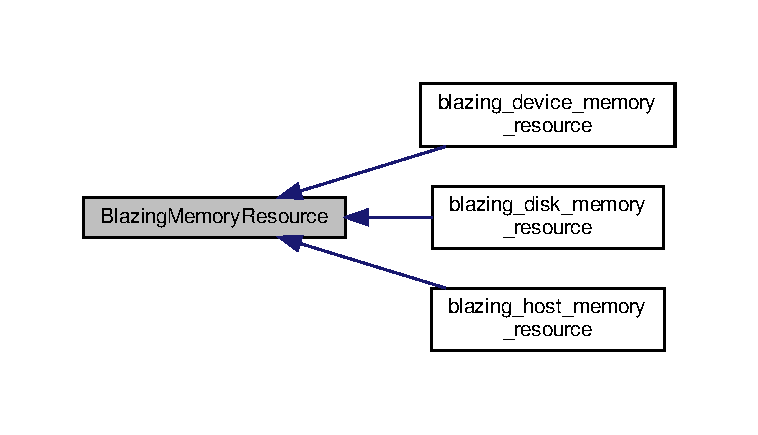
\includegraphics[width=350pt]{classBlazingMemoryResource__inherit__graph}
\end{center}
\end{figure}
\subsection*{Public Member Functions}
\begin{DoxyCompactItemize}
\item 
\mbox{\Hypertarget{classBlazingMemoryResource_abd562a80dbab3fd1d174f8e6ec4547f0}\label{classBlazingMemoryResource_abd562a80dbab3fd1d174f8e6ec4547f0}} 
virtual size\+\_\+t {\bfseries get\+\_\+from\+\_\+driver\+\_\+used\+\_\+memory} ()=0
\item 
\mbox{\Hypertarget{classBlazingMemoryResource_a1436e73e3554c721a5a972fcf21bc91f}\label{classBlazingMemoryResource_a1436e73e3554c721a5a972fcf21bc91f}} 
virtual size\+\_\+t {\bfseries get\+\_\+memory\+\_\+limit} ()=0
\item 
\mbox{\Hypertarget{classBlazingMemoryResource_a89e616e15446e4bfd013d55b714f1fc9}\label{classBlazingMemoryResource_a89e616e15446e4bfd013d55b714f1fc9}} 
virtual size\+\_\+t {\bfseries get\+\_\+memory\+\_\+used} ()=0
\item 
\mbox{\Hypertarget{classBlazingMemoryResource_a5e3c23ce2c2b065bed12f9b29a9976f6}\label{classBlazingMemoryResource_a5e3c23ce2c2b065bed12f9b29a9976f6}} 
virtual size\+\_\+t {\bfseries get\+\_\+total\+\_\+memory} ()=0
\end{DoxyCompactItemize}


\subsection{Detailed Description}
This interface represents a custom memory resource used in the cache system. The Cache Machines uses singleton references to device, host and disk memory resources. Each object of the Cache\+Machine class has knownlegde about the status of the memory resource by using {\ttfamily get\+\_\+memory\+\_\+limit} and {\ttfamily get\+\_\+memory\+\_\+used} methods. 

The documentation for this class was generated from the following file\+:\begin{DoxyCompactItemize}
\item 
/home/tom/\+Documents/programming/romulo\+\_\+blazingsql/blazingsql/engine/src/bmr/Blazing\+Memory\+Resource.\+h\end{DoxyCompactItemize}

\hypertarget{structBlazingMissingMetadataException}{}\section{Blazing\+Missing\+Metadata\+Exception Struct Reference}
\label{structBlazingMissingMetadataException}\index{Blazing\+Missing\+Metadata\+Exception@{Blazing\+Missing\+Metadata\+Exception}}


Inheritance diagram for Blazing\+Missing\+Metadata\+Exception\+:\nopagebreak
\begin{figure}[H]
\begin{center}
\leavevmode
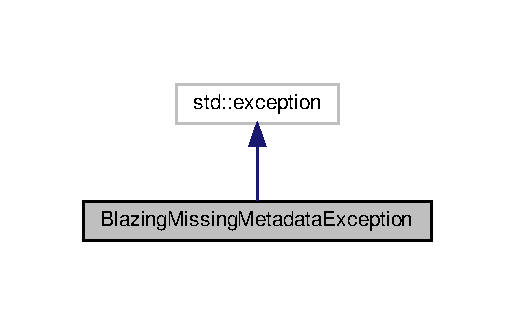
\includegraphics[width=247pt]{structBlazingMissingMetadataException__inherit__graph}
\end{center}
\end{figure}


Collaboration diagram for Blazing\+Missing\+Metadata\+Exception\+:\nopagebreak
\begin{figure}[H]
\begin{center}
\leavevmode
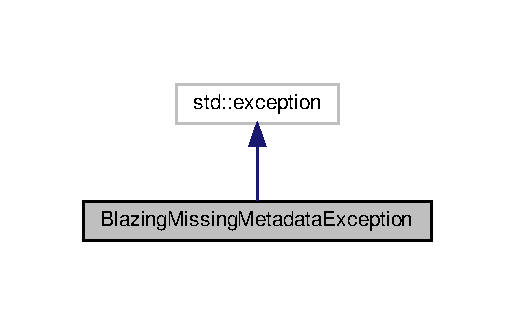
\includegraphics[width=247pt]{structBlazingMissingMetadataException__coll__graph}
\end{center}
\end{figure}
\subsection*{Public Member Functions}
\begin{DoxyCompactItemize}
\item 
\mbox{\Hypertarget{structBlazingMissingMetadataException_a5d6dac7b715ad5737b12999b41f36f4c}\label{structBlazingMissingMetadataException_a5d6dac7b715ad5737b12999b41f36f4c}} 
{\bfseries Blazing\+Missing\+Metadata\+Exception} (std\+::string key)
\item 
\mbox{\Hypertarget{structBlazingMissingMetadataException_a39eac0285bad513241cc214111206769}\label{structBlazingMissingMetadataException_a39eac0285bad513241cc214111206769}} 
const char $\ast$ {\bfseries what} () const  throw ()
\end{DoxyCompactItemize}


The documentation for this struct was generated from the following file\+:\begin{DoxyCompactItemize}
\item 
/home/tom/\+Documents/programming/romulo\+\_\+blazingsql/blazingsql/engine/src/error.\+hpp\end{DoxyCompactItemize}

\hypertarget{classral_1_1frame_1_1BlazingTable}{}\section{ral\+:\+:frame\+:\+:Blazing\+Table Class Reference}
\label{classral_1_1frame_1_1BlazingTable}\index{ral\+::frame\+::\+Blazing\+Table@{ral\+::frame\+::\+Blazing\+Table}}
\subsection*{Public Member Functions}
\begin{DoxyCompactItemize}
\item 
\mbox{\Hypertarget{classral_1_1frame_1_1BlazingTable_a7dbf7616b0bf068688b59031e6704408}\label{classral_1_1frame_1_1BlazingTable_a7dbf7616b0bf068688b59031e6704408}} 
{\bfseries Blazing\+Table} (std\+::vector$<$ std\+::unique\+\_\+ptr$<$ \hyperlink{classral_1_1frame_1_1BlazingColumn}{Blazing\+Column} $>$$>$ columns, const std\+::vector$<$ std\+::string $>$ \&column\+Names)
\item 
\mbox{\Hypertarget{classral_1_1frame_1_1BlazingTable_a77d0dda2ad02f3c2a6aacfb84e06a4a6}\label{classral_1_1frame_1_1BlazingTable_a77d0dda2ad02f3c2a6aacfb84e06a4a6}} 
{\bfseries Blazing\+Table} (std\+::unique\+\_\+ptr$<$ Cudf\+Table $>$ table, const std\+::vector$<$ std\+::string $>$ \&column\+Names)
\item 
\mbox{\Hypertarget{classral_1_1frame_1_1BlazingTable_ac6af86b8968e2f56a7bcb39c35fcd589}\label{classral_1_1frame_1_1BlazingTable_ac6af86b8968e2f56a7bcb39c35fcd589}} 
{\bfseries Blazing\+Table} (const Cudf\+Table\+View \&table, const std\+::vector$<$ std\+::string $>$ \&column\+Names)
\item 
\mbox{\Hypertarget{classral_1_1frame_1_1BlazingTable_a1fe4f1d3a9d95e8eba30dd723d318eb3}\label{classral_1_1frame_1_1BlazingTable_a1fe4f1d3a9d95e8eba30dd723d318eb3}} 
{\bfseries Blazing\+Table} (\hyperlink{classral_1_1frame_1_1BlazingTable}{Blazing\+Table} \&\&)=default
\item 
\mbox{\Hypertarget{classral_1_1frame_1_1BlazingTable_a4dc7d75cc8598f067267a9ab9bfdccb9}\label{classral_1_1frame_1_1BlazingTable_a4dc7d75cc8598f067267a9ab9bfdccb9}} 
\hyperlink{classral_1_1frame_1_1BlazingTable}{Blazing\+Table} \& {\bfseries operator=} (\hyperlink{classral_1_1frame_1_1BlazingTable}{Blazing\+Table} const \&)=delete
\item 
\mbox{\Hypertarget{classral_1_1frame_1_1BlazingTable_af103b98ebd31e68f7b68e39c3a7e9dd2}\label{classral_1_1frame_1_1BlazingTable_af103b98ebd31e68f7b68e39c3a7e9dd2}} 
\hyperlink{classral_1_1frame_1_1BlazingTable}{Blazing\+Table} \& {\bfseries operator=} (\hyperlink{classral_1_1frame_1_1BlazingTable}{Blazing\+Table} \&\&)=delete
\item 
\mbox{\Hypertarget{classral_1_1frame_1_1BlazingTable_abc7e37ec7cb9e41e59c82cf39aa78c90}\label{classral_1_1frame_1_1BlazingTable_abc7e37ec7cb9e41e59c82cf39aa78c90}} 
Cudf\+Table\+View {\bfseries view} () const
\item 
\mbox{\Hypertarget{classral_1_1frame_1_1BlazingTable_a71e54c253edfbc147685b444011cb3e9}\label{classral_1_1frame_1_1BlazingTable_a71e54c253edfbc147685b444011cb3e9}} 
cudf\+::size\+\_\+type {\bfseries num\+\_\+columns} () const
\item 
\mbox{\Hypertarget{classral_1_1frame_1_1BlazingTable_a4a294d20b7502f18c224213b93c0667c}\label{classral_1_1frame_1_1BlazingTable_a4a294d20b7502f18c224213b93c0667c}} 
cudf\+::size\+\_\+type {\bfseries num\+\_\+rows} () const
\item 
\mbox{\Hypertarget{classral_1_1frame_1_1BlazingTable_acd43177a0839463a582a8aeab59a860a}\label{classral_1_1frame_1_1BlazingTable_acd43177a0839463a582a8aeab59a860a}} 
std\+::vector$<$ std\+::string $>$ {\bfseries names} () const
\item 
\mbox{\Hypertarget{classral_1_1frame_1_1BlazingTable_afc57e3dea4ebf9167ec7900c44a14c27}\label{classral_1_1frame_1_1BlazingTable_afc57e3dea4ebf9167ec7900c44a14c27}} 
std\+::vector$<$ cudf\+::data\+\_\+type $>$ {\bfseries get\+\_\+schema} () const
\item 
\mbox{\Hypertarget{classral_1_1frame_1_1BlazingTable_a9272855bd4e0c0253e0389a0d108d947}\label{classral_1_1frame_1_1BlazingTable_a9272855bd4e0c0253e0389a0d108d947}} 
void {\bfseries set\+Names} (const std\+::vector$<$ std\+::string $>$ \&names)
\item 
\mbox{\Hypertarget{classral_1_1frame_1_1BlazingTable_adee9be4f7f57023e69c069b9c1564a88}\label{classral_1_1frame_1_1BlazingTable_adee9be4f7f57023e69c069b9c1564a88}} 
\hyperlink{classral_1_1frame_1_1BlazingTableView}{Blazing\+Table\+View} {\bfseries to\+Blazing\+Table\+View} () const
\item 
\mbox{\Hypertarget{classral_1_1frame_1_1BlazingTable_a1385de902ecdddf68622215cd72bb22b}\label{classral_1_1frame_1_1BlazingTable_a1385de902ecdddf68622215cd72bb22b}} 
{\bfseries operator bool} () const
\item 
\mbox{\Hypertarget{classral_1_1frame_1_1BlazingTable_ac0c7e71526645b690d49d24d563358ef}\label{classral_1_1frame_1_1BlazingTable_ac0c7e71526645b690d49d24d563358ef}} 
bool {\bfseries is\+\_\+valid} () const
\item 
\mbox{\Hypertarget{classral_1_1frame_1_1BlazingTable_a45851d20f39300385437d51c22e413ec}\label{classral_1_1frame_1_1BlazingTable_a45851d20f39300385437d51c22e413ec}} 
std\+::unique\+\_\+ptr$<$ Cudf\+Table $>$ {\bfseries release\+Cudf\+Table} ()
\item 
\mbox{\Hypertarget{classral_1_1frame_1_1BlazingTable_a9e98b23e48ed6ce63a7b059dbc4de296}\label{classral_1_1frame_1_1BlazingTable_a9e98b23e48ed6ce63a7b059dbc4de296}} 
std\+::vector$<$ std\+::unique\+\_\+ptr$<$ \hyperlink{classral_1_1frame_1_1BlazingColumn}{Blazing\+Column} $>$ $>$ {\bfseries release\+Blazing\+Columns} ()
\item 
\mbox{\Hypertarget{classral_1_1frame_1_1BlazingTable_a990ef8ca85622d9a8fade035159c77b4}\label{classral_1_1frame_1_1BlazingTable_a990ef8ca85622d9a8fade035159c77b4}} 
unsigned long long {\bfseries size\+In\+Bytes} ()
\item 
\mbox{\Hypertarget{classral_1_1frame_1_1BlazingTable_a2a1a2e6cd939fe3ead68b2c913647087}\label{classral_1_1frame_1_1BlazingTable_a2a1a2e6cd939fe3ead68b2c913647087}} 
void {\bfseries ensure\+Ownership} ()
\end{DoxyCompactItemize}


The documentation for this class was generated from the following files\+:\begin{DoxyCompactItemize}
\item 
/home/tom/\+Documents/programming/romulo\+\_\+blazingsql/blazingsql/engine/src/execution\+\_\+graph/logic\+\_\+controllers/Logic\+Primitives.\+h\item 
/home/tom/\+Documents/programming/romulo\+\_\+blazingsql/blazingsql/engine/src/execution\+\_\+graph/logic\+\_\+controllers/Logic\+Primitives.\+cpp\end{DoxyCompactItemize}

\hypertarget{classral_1_1frame_1_1BlazingTableView}{}\section{ral\+:\+:frame\+:\+:Blazing\+Table\+View Class Reference}
\label{classral_1_1frame_1_1BlazingTableView}\index{ral\+::frame\+::\+Blazing\+Table\+View@{ral\+::frame\+::\+Blazing\+Table\+View}}
\subsection*{Public Member Functions}
\begin{DoxyCompactItemize}
\item 
\mbox{\Hypertarget{classral_1_1frame_1_1BlazingTableView_aef63d115fc7d2cadcf2e2c811388b48d}\label{classral_1_1frame_1_1BlazingTableView_aef63d115fc7d2cadcf2e2c811388b48d}} 
{\bfseries Blazing\+Table\+View} (Cudf\+Table\+View table, std\+::vector$<$ std\+::string $>$ column\+Names)
\item 
\mbox{\Hypertarget{classral_1_1frame_1_1BlazingTableView_aa5395f0a1a0bda5fa44ffb36b40f6e5a}\label{classral_1_1frame_1_1BlazingTableView_aa5395f0a1a0bda5fa44ffb36b40f6e5a}} 
{\bfseries Blazing\+Table\+View} (\hyperlink{classral_1_1frame_1_1BlazingTableView}{Blazing\+Table\+View} const \&)=default
\item 
\mbox{\Hypertarget{classral_1_1frame_1_1BlazingTableView_a3ac765c7829f2aef5d563ae24a305dea}\label{classral_1_1frame_1_1BlazingTableView_a3ac765c7829f2aef5d563ae24a305dea}} 
{\bfseries Blazing\+Table\+View} (\hyperlink{classral_1_1frame_1_1BlazingTableView}{Blazing\+Table\+View} \&\&)=default
\item 
\mbox{\Hypertarget{classral_1_1frame_1_1BlazingTableView_a67c2fada551518d1026b3bf81851b5e6}\label{classral_1_1frame_1_1BlazingTableView_a67c2fada551518d1026b3bf81851b5e6}} 
\hyperlink{classral_1_1frame_1_1BlazingTableView}{Blazing\+Table\+View} \& {\bfseries operator=} (\hyperlink{classral_1_1frame_1_1BlazingTableView}{Blazing\+Table\+View} const \&)=default
\item 
\mbox{\Hypertarget{classral_1_1frame_1_1BlazingTableView_a054fa47daa382903e253d2c2963dd68a}\label{classral_1_1frame_1_1BlazingTableView_a054fa47daa382903e253d2c2963dd68a}} 
\hyperlink{classral_1_1frame_1_1BlazingTableView}{Blazing\+Table\+View} \& {\bfseries operator=} (\hyperlink{classral_1_1frame_1_1BlazingTableView}{Blazing\+Table\+View} \&\&)=default
\item 
\mbox{\Hypertarget{classral_1_1frame_1_1BlazingTableView_a5aa2bb6c557193c1ce9ffc6f4fe11bff}\label{classral_1_1frame_1_1BlazingTableView_a5aa2bb6c557193c1ce9ffc6f4fe11bff}} 
Cudf\+Table\+View {\bfseries view} () const
\item 
\mbox{\Hypertarget{classral_1_1frame_1_1BlazingTableView_a7883b53092571ae6bdbf2994c8099686}\label{classral_1_1frame_1_1BlazingTableView_a7883b53092571ae6bdbf2994c8099686}} 
cudf\+::column\+\_\+view const  \& {\bfseries column} (cudf\+::size\+\_\+type column\+\_\+index) const
\item 
\mbox{\Hypertarget{classral_1_1frame_1_1BlazingTableView_a29cd66a4f4da704e455bf34b21a1c64a}\label{classral_1_1frame_1_1BlazingTableView_a29cd66a4f4da704e455bf34b21a1c64a}} 
std\+::vector$<$ std\+::unique\+\_\+ptr$<$ \hyperlink{classral_1_1frame_1_1BlazingColumn}{Blazing\+Column} $>$ $>$ {\bfseries to\+Blazing\+Columns} () const
\item 
\mbox{\Hypertarget{classral_1_1frame_1_1BlazingTableView_afcebfe01ec7db42b859bf6598f65a3f5}\label{classral_1_1frame_1_1BlazingTableView_afcebfe01ec7db42b859bf6598f65a3f5}} 
std\+::vector$<$ cudf\+::data\+\_\+type $>$ {\bfseries get\+\_\+schema} () const
\item 
\mbox{\Hypertarget{classral_1_1frame_1_1BlazingTableView_a6b6d93945df55aed6cc1039bcb3743b3}\label{classral_1_1frame_1_1BlazingTableView_a6b6d93945df55aed6cc1039bcb3743b3}} 
std\+::vector$<$ std\+::string $>$ {\bfseries names} () const
\item 
\mbox{\Hypertarget{classral_1_1frame_1_1BlazingTableView_aff8c4df40002de33aa4b176daaa8e1c0}\label{classral_1_1frame_1_1BlazingTableView_aff8c4df40002de33aa4b176daaa8e1c0}} 
void {\bfseries set\+Names} (const std\+::vector$<$ std\+::string $>$ \&names)
\item 
\mbox{\Hypertarget{classral_1_1frame_1_1BlazingTableView_ae239be70b79bcafb195d6e8850655162}\label{classral_1_1frame_1_1BlazingTableView_ae239be70b79bcafb195d6e8850655162}} 
cudf\+::size\+\_\+type {\bfseries num\+\_\+columns} () const
\item 
\mbox{\Hypertarget{classral_1_1frame_1_1BlazingTableView_a39ab4d3e5b6df35263e890032ca943e7}\label{classral_1_1frame_1_1BlazingTableView_a39ab4d3e5b6df35263e890032ca943e7}} 
cudf\+::size\+\_\+type {\bfseries num\+\_\+rows} () const
\item 
\mbox{\Hypertarget{classral_1_1frame_1_1BlazingTableView_adf6a6ea945a422b25beb46ec7c21d863}\label{classral_1_1frame_1_1BlazingTableView_adf6a6ea945a422b25beb46ec7c21d863}} 
unsigned long long {\bfseries size\+In\+Bytes} ()
\item 
\mbox{\Hypertarget{classral_1_1frame_1_1BlazingTableView_a0243487937ce1de435ad96562f12f814}\label{classral_1_1frame_1_1BlazingTableView_a0243487937ce1de435ad96562f12f814}} 
std\+::unique\+\_\+ptr$<$ \hyperlink{classral_1_1frame_1_1BlazingTable}{Blazing\+Table} $>$ {\bfseries clone} () const
\end{DoxyCompactItemize}


The documentation for this class was generated from the following files\+:\begin{DoxyCompactItemize}
\item 
/home/tom/\+Documents/programming/romulo\+\_\+blazingsql/blazingsql/engine/src/execution\+\_\+graph/logic\+\_\+controllers/Logic\+Primitives.\+h\item 
/home/tom/\+Documents/programming/romulo\+\_\+blazingsql/blazingsql/engine/src/execution\+\_\+graph/logic\+\_\+controllers/Logic\+Primitives.\+cpp\end{DoxyCompactItemize}

\hypertarget{classral_1_1memory_1_1buffer__providers}{}\section{ral\+:\+:memory\+:\+:buffer\+\_\+providers Class Reference}
\label{classral_1_1memory_1_1buffer__providers}\index{ral\+::memory\+::buffer\+\_\+providers@{ral\+::memory\+::buffer\+\_\+providers}}


This class represents the buffer providers used by the engine.  




{\ttfamily \#include $<$Buffer\+Provider.\+h$>$}

\subsection*{Static Public Member Functions}
\begin{DoxyCompactItemize}
\item 
\mbox{\Hypertarget{classral_1_1memory_1_1buffer__providers_af3457404f12257d5063ad7bc435a465b}\label{classral_1_1memory_1_1buffer__providers_af3457404f12257d5063ad7bc435a465b}} 
static std\+::shared\+\_\+ptr$<$ \hyperlink{classral_1_1memory_1_1allocation__pool}{allocation\+\_\+pool} $>$ \& {\bfseries get\+\_\+host\+\_\+buffer\+\_\+provider} ()
\item 
\mbox{\Hypertarget{classral_1_1memory_1_1buffer__providers_a2dd6153c40c21af29056fa00883bde21}\label{classral_1_1memory_1_1buffer__providers_a2dd6153c40c21af29056fa00883bde21}} 
static std\+::shared\+\_\+ptr$<$ \hyperlink{classral_1_1memory_1_1allocation__pool}{allocation\+\_\+pool} $>$ \& {\bfseries get\+\_\+pinned\+\_\+buffer\+\_\+provider} ()
\end{DoxyCompactItemize}


\subsection{Detailed Description}
This class represents the buffer providers used by the engine. 

\begin{DoxyNote}{Note}
Myers\textquotesingle{} singleton. Thread safe and unique. Note\+: C++11 required. 
\end{DoxyNote}


The documentation for this class was generated from the following file\+:\begin{DoxyCompactItemize}
\item 
/home/tom/\+Documents/programming/romulo\+\_\+blazingsql/blazingsql/engine/src/bmr/Buffer\+Provider.\+h\end{DoxyCompactItemize}

\hypertarget{classcomm_1_1buffer__transport}{}\section{comm\+:\+:buffer\+\_\+transport Class Reference}
\label{classcomm_1_1buffer__transport}\index{comm\+::buffer\+\_\+transport@{comm\+::buffer\+\_\+transport}}


Base class used to send a chunk of bytes throught a transport protocol e.\+g. T\+CP, U\+CP, etc.  




{\ttfamily \#include $<$buffer\+Transport.\+hpp$>$}



Inheritance diagram for comm\+:\+:buffer\+\_\+transport\+:\nopagebreak
\begin{figure}[H]
\begin{center}
\leavevmode
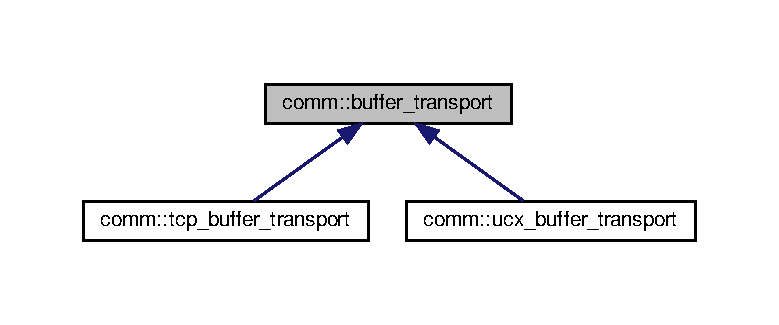
\includegraphics[width=350pt]{classcomm_1_1buffer__transport__inherit__graph}
\end{center}
\end{figure}


Collaboration diagram for comm\+:\+:buffer\+\_\+transport\+:\nopagebreak
\begin{figure}[H]
\begin{center}
\leavevmode
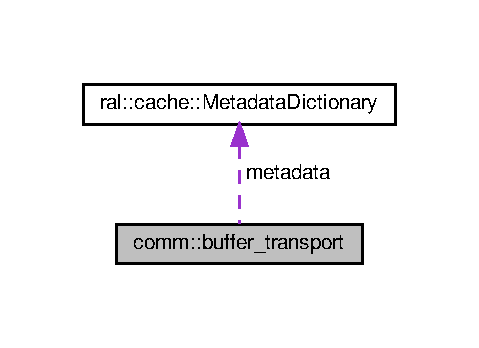
\includegraphics[width=230pt]{classcomm_1_1buffer__transport__coll__graph}
\end{center}
\end{figure}
\subsection*{Public Member Functions}
\begin{DoxyCompactItemize}
\item 
\hyperlink{classcomm_1_1buffer__transport_a012bb1c7d1f7a2e9512815cafd95ef80}{buffer\+\_\+transport} (\hyperlink{classral_1_1cache_1_1MetadataDictionary}{ral\+::cache\+::\+Metadata\+Dictionary} metadata, std\+::vector$<$ size\+\_\+t $>$ buffer\+\_\+sizes, std\+::vector$<$ \hyperlink{structblazingdb_1_1transport_1_1ColumnTransport}{blazingdb\+::transport\+::\+Column\+Transport} $>$ column\+\_\+transports, std\+::vector$<$ \hyperlink{structral_1_1memory_1_1blazing__chunked__column__info}{ral\+::memory\+::blazing\+\_\+chunked\+\_\+column\+\_\+info} $>$ chunked\+\_\+column\+\_\+infos, std\+::vector$<$ \hyperlink{classcomm_1_1node}{node} $>$ destinations, bool require\+\_\+acknowledge)
\begin{DoxyCompactList}\small\item\em Constructs a \hyperlink{classcomm_1_1buffer__transport}{buffer\+\_\+transport}. \end{DoxyCompactList}\item 
\mbox{\Hypertarget{classcomm_1_1buffer__transport_a0ea6dd0f6412b2422cc47706ad34dad9}\label{classcomm_1_1buffer__transport_a0ea6dd0f6412b2422cc47706ad34dad9}} 
virtual void {\bfseries send\+\_\+begin\+\_\+transmission} ()=0
\item 
void \hyperlink{classcomm_1_1buffer__transport_a0a7ae6691d0a182c4567f3001f96aefe}{send} (const char $\ast$buffer, size\+\_\+t buffer\+\_\+size)
\begin{DoxyCompactList}\small\item\em Sends a chunk of bytes throught a transport protocol. \end{DoxyCompactList}\item 
\mbox{\Hypertarget{classcomm_1_1buffer__transport_aef710177ed4367311b1d8e70acead7c2}\label{classcomm_1_1buffer__transport_aef710177ed4367311b1d8e70acead7c2}} 
void \hyperlink{classcomm_1_1buffer__transport_aef710177ed4367311b1d8e70acead7c2}{wait\+\_\+until\+\_\+complete} ()
\begin{DoxyCompactList}\small\item\em Waits until all the data is sents. \end{DoxyCompactList}\item 
\mbox{\Hypertarget{classcomm_1_1buffer__transport_a6388e67a79f9a5c2e80ed45b23e6327c}\label{classcomm_1_1buffer__transport_a6388e67a79f9a5c2e80ed45b23e6327c}} 
void {\bfseries wait\+\_\+for\+\_\+begin\+\_\+transmission} ()
\item 
\mbox{\Hypertarget{classcomm_1_1buffer__transport_a3b921d1808fb74d95f83146de5269cb6}\label{classcomm_1_1buffer__transport_a3b921d1808fb74d95f83146de5269cb6}} 
virtual void {\bfseries increment\+\_\+frame\+\_\+transmission} ()
\item 
\mbox{\Hypertarget{classcomm_1_1buffer__transport_a81080122f0355dae745d7bf6453152a8}\label{classcomm_1_1buffer__transport_a81080122f0355dae745d7bf6453152a8}} 
virtual void {\bfseries increment\+\_\+begin\+\_\+transmission} ()
\end{DoxyCompactItemize}
\subsection*{Protected Member Functions}
\begin{DoxyCompactItemize}
\item 
\mbox{\Hypertarget{classcomm_1_1buffer__transport_a7c4d1651a8af5965619c9e37b225859d}\label{classcomm_1_1buffer__transport_a7c4d1651a8af5965619c9e37b225859d}} 
virtual void {\bfseries send\+\_\+impl} (const char $\ast$buffer, size\+\_\+t buffer\+\_\+size)=0
\item 
\mbox{\Hypertarget{classcomm_1_1buffer__transport_a6aa1fb3a4543ace7e5c06914252a02e4}\label{classcomm_1_1buffer__transport_a6aa1fb3a4543ace7e5c06914252a02e4}} 
virtual void {\bfseries receive\+\_\+acknowledge} ()=0
\end{DoxyCompactItemize}
\subsection*{Protected Attributes}
\begin{DoxyCompactItemize}
\item 
\mbox{\Hypertarget{classcomm_1_1buffer__transport_ad5104419e3ecfca874534e12804b48fc}\label{classcomm_1_1buffer__transport_ad5104419e3ecfca874534e12804b48fc}} 
std\+::vector$<$ \hyperlink{structblazingdb_1_1transport_1_1ColumnTransport}{blazingdb\+::transport\+::\+Column\+Transport} $>$ {\bfseries column\+\_\+transports}
\item 
\mbox{\Hypertarget{classcomm_1_1buffer__transport_aa02f7f37ea5c8c4343e3289d6b9e132c}\label{classcomm_1_1buffer__transport_aa02f7f37ea5c8c4343e3289d6b9e132c}} 
std\+::vector$<$ \hyperlink{structral_1_1memory_1_1blazing__chunked__column__info}{ral\+::memory\+::blazing\+\_\+chunked\+\_\+column\+\_\+info} $>$ {\bfseries chunked\+\_\+column\+\_\+infos}
\item 
\mbox{\Hypertarget{classcomm_1_1buffer__transport_a0b3c07ac433f3c7b114e677f399e3210}\label{classcomm_1_1buffer__transport_a0b3c07ac433f3c7b114e677f399e3210}} 
\hyperlink{classral_1_1cache_1_1MetadataDictionary}{ral\+::cache\+::\+Metadata\+Dictionary} {\bfseries metadata}
\item 
\mbox{\Hypertarget{classcomm_1_1buffer__transport_ae01314b9b03cd1278a20996dafc4dcb0}\label{classcomm_1_1buffer__transport_ae01314b9b03cd1278a20996dafc4dcb0}} 
std\+::vector$<$ size\+\_\+t $>$ {\bfseries buffer\+\_\+sizes}
\item 
\mbox{\Hypertarget{classcomm_1_1buffer__transport_a3bf404422bf786f01a45066f48a751c6}\label{classcomm_1_1buffer__transport_a3bf404422bf786f01a45066f48a751c6}} 
size\+\_\+t {\bfseries buffer\+\_\+sent} = 0
\item 
std\+::atomic$<$ size\+\_\+t $>$ \hyperlink{classcomm_1_1buffer__transport_af9c04a8af736e05980d62b7448142b30}{transmitted\+\_\+begin\+\_\+frames}
\item 
std\+::atomic$<$ size\+\_\+t $>$ \hyperlink{classcomm_1_1buffer__transport_a1c8254316bfcb05204a196bece986f68}{transmitted\+\_\+frames}
\item 
\mbox{\Hypertarget{classcomm_1_1buffer__transport_aaef40e35a9a214ecb83d44493937449e}\label{classcomm_1_1buffer__transport_aaef40e35a9a214ecb83d44493937449e}} 
std\+::mutex {\bfseries mutex}
\item 
\mbox{\Hypertarget{classcomm_1_1buffer__transport_a57085a949db7cafedccdd6ce8db29b9e}\label{classcomm_1_1buffer__transport_a57085a949db7cafedccdd6ce8db29b9e}} 
std\+::condition\+\_\+variable {\bfseries completion\+\_\+condition\+\_\+variable}
\item 
\mbox{\Hypertarget{classcomm_1_1buffer__transport_a625bc455a5fc03c79cb4501c6b993aa8}\label{classcomm_1_1buffer__transport_a625bc455a5fc03c79cb4501c6b993aa8}} 
std\+::vector$<$ \hyperlink{classcomm_1_1node}{node} $>$ {\bfseries destinations}
\item 
\mbox{\Hypertarget{classcomm_1_1buffer__transport_a22e84756f6b66324df67bdd556600c19}\label{classcomm_1_1buffer__transport_a22e84756f6b66324df67bdd556600c19}} 
std\+::map$<$ std\+::string, bool $>$ {\bfseries transmitted\+\_\+acknowledgements}
\item 
\mbox{\Hypertarget{classcomm_1_1buffer__transport_a089d28bc6f8f3eac8a89705bd7391a30}\label{classcomm_1_1buffer__transport_a089d28bc6f8f3eac8a89705bd7391a30}} 
bool {\bfseries require\+\_\+acknowledge} = false
\end{DoxyCompactItemize}


\subsection{Detailed Description}
Base class used to send a chunk of bytes throught a transport protocol e.\+g. T\+CP, U\+CP, etc. 

\subsection{Constructor \& Destructor Documentation}
\mbox{\Hypertarget{classcomm_1_1buffer__transport_a012bb1c7d1f7a2e9512815cafd95ef80}\label{classcomm_1_1buffer__transport_a012bb1c7d1f7a2e9512815cafd95ef80}} 
\index{comm\+::buffer\+\_\+transport@{comm\+::buffer\+\_\+transport}!buffer\+\_\+transport@{buffer\+\_\+transport}}
\index{buffer\+\_\+transport@{buffer\+\_\+transport}!comm\+::buffer\+\_\+transport@{comm\+::buffer\+\_\+transport}}
\subsubsection{\texorpdfstring{buffer\+\_\+transport()}{buffer\_transport()}}
{\footnotesize\ttfamily comm\+::buffer\+\_\+transport\+::buffer\+\_\+transport (\begin{DoxyParamCaption}\item[{\hyperlink{classral_1_1cache_1_1MetadataDictionary}{ral\+::cache\+::\+Metadata\+Dictionary}}]{metadata,  }\item[{std\+::vector$<$ size\+\_\+t $>$}]{buffer\+\_\+sizes,  }\item[{std\+::vector$<$ \hyperlink{structblazingdb_1_1transport_1_1ColumnTransport}{blazingdb\+::transport\+::\+Column\+Transport} $>$}]{column\+\_\+transports,  }\item[{std\+::vector$<$ \hyperlink{structral_1_1memory_1_1blazing__chunked__column__info}{ral\+::memory\+::blazing\+\_\+chunked\+\_\+column\+\_\+info} $>$}]{chunked\+\_\+column\+\_\+infos,  }\item[{std\+::vector$<$ \hyperlink{classcomm_1_1node}{node} $>$}]{destinations,  }\item[{bool}]{require\+\_\+acknowledge }\end{DoxyParamCaption})}



Constructs a \hyperlink{classcomm_1_1buffer__transport}{buffer\+\_\+transport}. 


\begin{DoxyParams}{Parameters}
{\em metadata} & This is information about how the message was routed and payloads that are used in execution, planning, or physical optimizations. E.\+G. num rows in table, num partitions to be processed \\
\hline
{\em buffer\+\_\+sizes} & A vector containing the sizes of the buffer \\
\hline
{\em column\+\_\+transports} & A vector of Column\+Transport representing column metadata \\
\hline
{\em chunked\+\_\+column\+\_\+infos} & A vector of blazing\+\_\+chunked\+\_\+column\+\_\+info representing how the raw buffers are chunked \\
\hline
{\em destinations} & A vector of destination nodes \\
\hline
{\em require\+\_\+acknowledge} & A boolean stating if acknowledgement of a message is required \\
\hline
\end{DoxyParams}


\subsection{Member Function Documentation}
\mbox{\Hypertarget{classcomm_1_1buffer__transport_a0a7ae6691d0a182c4567f3001f96aefe}\label{classcomm_1_1buffer__transport_a0a7ae6691d0a182c4567f3001f96aefe}} 
\index{comm\+::buffer\+\_\+transport@{comm\+::buffer\+\_\+transport}!send@{send}}
\index{send@{send}!comm\+::buffer\+\_\+transport@{comm\+::buffer\+\_\+transport}}
\subsubsection{\texorpdfstring{send()}{send()}}
{\footnotesize\ttfamily void comm\+::buffer\+\_\+transport\+::send (\begin{DoxyParamCaption}\item[{const char $\ast$}]{buffer,  }\item[{size\+\_\+t}]{buffer\+\_\+size }\end{DoxyParamCaption})}



Sends a chunk of bytes throught a transport protocol. 


\begin{DoxyParams}{Parameters}
{\em buffer} & Pointer to the byte buffer that will be send \\
\hline
{\em buffer\+\_\+size} & The buffer size \\
\hline
\end{DoxyParams}


\subsection{Member Data Documentation}
\mbox{\Hypertarget{classcomm_1_1buffer__transport_af9c04a8af736e05980d62b7448142b30}\label{classcomm_1_1buffer__transport_af9c04a8af736e05980d62b7448142b30}} 
\index{comm\+::buffer\+\_\+transport@{comm\+::buffer\+\_\+transport}!transmitted\+\_\+begin\+\_\+frames@{transmitted\+\_\+begin\+\_\+frames}}
\index{transmitted\+\_\+begin\+\_\+frames@{transmitted\+\_\+begin\+\_\+frames}!comm\+::buffer\+\_\+transport@{comm\+::buffer\+\_\+transport}}
\subsubsection{\texorpdfstring{transmitted\+\_\+begin\+\_\+frames}{transmitted\_begin\_frames}}
{\footnotesize\ttfamily std\+::atomic$<$size\+\_\+t$>$ comm\+::buffer\+\_\+transport\+::transmitted\+\_\+begin\+\_\+frames\hspace{0.3cm}{\ttfamily [protected]}}

The number of begin\+\_\+transmission messages sent \mbox{\Hypertarget{classcomm_1_1buffer__transport_a1c8254316bfcb05204a196bece986f68}\label{classcomm_1_1buffer__transport_a1c8254316bfcb05204a196bece986f68}} 
\index{comm\+::buffer\+\_\+transport@{comm\+::buffer\+\_\+transport}!transmitted\+\_\+frames@{transmitted\+\_\+frames}}
\index{transmitted\+\_\+frames@{transmitted\+\_\+frames}!comm\+::buffer\+\_\+transport@{comm\+::buffer\+\_\+transport}}
\subsubsection{\texorpdfstring{transmitted\+\_\+frames}{transmitted\_frames}}
{\footnotesize\ttfamily std\+::atomic$<$size\+\_\+t$>$ comm\+::buffer\+\_\+transport\+::transmitted\+\_\+frames\hspace{0.3cm}{\ttfamily [protected]}}

The number of frames transmitted 

The documentation for this class was generated from the following files\+:\begin{DoxyCompactItemize}
\item 
/home/tom/\+Documents/programming/romulo\+\_\+blazingsql/blazingsql/engine/src/communication/\+Communication\+Interface/buffer\+Transport.\+hpp\item 
/home/tom/\+Documents/programming/romulo\+\_\+blazingsql/blazingsql/engine/src/communication/\+Communication\+Interface/buffer\+Transport.\+cpp\end{DoxyCompactItemize}

\hypertarget{structral_1_1cache_1_1cache__settings}{}\section{ral\+:\+:cache\+:\+:cache\+\_\+settings Struct Reference}
\label{structral_1_1cache_1_1cache__settings}\index{ral\+::cache\+::cache\+\_\+settings@{ral\+::cache\+::cache\+\_\+settings}}


An object that represent a cache machine configuration (type and num\+\_\+partitions) used in create\+\_\+cache\+\_\+machine and create\+\_\+cache\+\_\+machine functions.  




{\ttfamily \#include $<$kpair.\+h$>$}

\subsection*{Public Attributes}
\begin{DoxyCompactItemize}
\item 
\mbox{\Hypertarget{structral_1_1cache_1_1cache__settings_a9b3e3c655751cd121cd5a6ed169c0be0}\label{structral_1_1cache_1_1cache__settings_a9b3e3c655751cd121cd5a6ed169c0be0}} 
Cache\+Type {\bfseries type} = Cache\+Type\+::\+S\+I\+M\+P\+LE
\item 
\mbox{\Hypertarget{structral_1_1cache_1_1cache__settings_a20bbad604695b4a4e97f0e53c4c99178}\label{structral_1_1cache_1_1cache__settings_a20bbad604695b4a4e97f0e53c4c99178}} 
int {\bfseries num\+\_\+partitions} = 1
\item 
\mbox{\Hypertarget{structral_1_1cache_1_1cache__settings_aa9cc6ee9667f1aaf89e03952f8a2a822}\label{structral_1_1cache_1_1cache__settings_aa9cc6ee9667f1aaf89e03952f8a2a822}} 
std\+::shared\+\_\+ptr$<$ \hyperlink{classblazingdb_1_1manager_1_1Context}{Context} $>$ {\bfseries context}
\item 
\mbox{\Hypertarget{structral_1_1cache_1_1cache__settings_a6d157349c6a1c19fe1c4d0368814fb70}\label{structral_1_1cache_1_1cache__settings_a6d157349c6a1c19fe1c4d0368814fb70}} 
std\+::size\+\_\+t {\bfseries concat\+\_\+cache\+\_\+num\+\_\+bytes} = 400000000
\item 
\mbox{\Hypertarget{structral_1_1cache_1_1cache__settings_acac908087611fef1560d36be68f1e418}\label{structral_1_1cache_1_1cache__settings_acac908087611fef1560d36be68f1e418}} 
bool \hyperlink{structral_1_1cache_1_1cache__settings_acac908087611fef1560d36be68f1e418}{concat\+\_\+all} = false
\begin{DoxyCompactList}\small\item\em Applicable only for concatenating caches. \end{DoxyCompactList}\end{DoxyCompactItemize}


\subsection{Detailed Description}
An object that represent a cache machine configuration (type and num\+\_\+partitions) used in create\+\_\+cache\+\_\+machine and create\+\_\+cache\+\_\+machine functions. 

The documentation for this struct was generated from the following file\+:\begin{DoxyCompactItemize}
\item 
/home/tom/\+Documents/programming/romulo\+\_\+blazingsql/blazingsql/engine/src/execution\+\_\+graph/logic\+\_\+controllers/taskflow/kpair.\+h\end{DoxyCompactItemize}

\hypertarget{classral_1_1cache_1_1CacheData}{}\section{ral\+:\+:cache\+:\+:Cache\+Data Class Reference}
\label{classral_1_1cache_1_1CacheData}\index{ral\+::cache\+::\+Cache\+Data@{ral\+::cache\+::\+Cache\+Data}}


{\ttfamily \#include $<$Cache\+Data.\+h$>$}



Inheritance diagram for ral\+:\+:cache\+:\+:Cache\+Data\+:\nopagebreak
\begin{figure}[H]
\begin{center}
\leavevmode
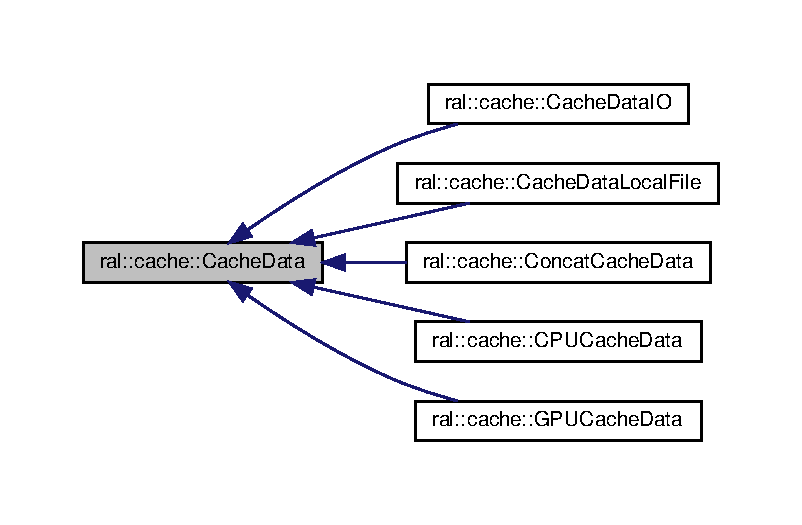
\includegraphics[width=350pt]{classral_1_1cache_1_1CacheData__inherit__graph}
\end{center}
\end{figure}


Collaboration diagram for ral\+:\+:cache\+:\+:Cache\+Data\+:\nopagebreak
\begin{figure}[H]
\begin{center}
\leavevmode
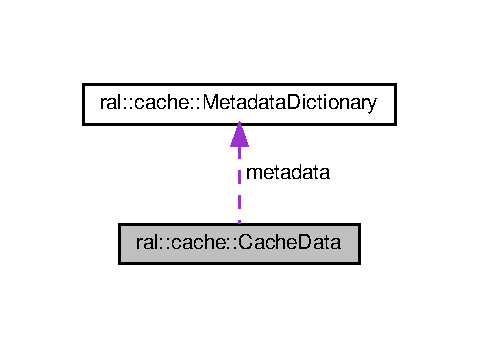
\includegraphics[width=230pt]{classral_1_1cache_1_1CacheData__coll__graph}
\end{center}
\end{figure}
\subsection*{Public Member Functions}
\begin{DoxyCompactItemize}
\item 
\hyperlink{classral_1_1cache_1_1CacheData_a257a4e0a13e894093e8ae37da1612c62}{Cache\+Data} (Cache\+Data\+Type \hyperlink{classral_1_1cache_1_1CacheData_acf9d130e22baac61d4689c52e36b9c17}{cache\+\_\+type}, std\+::vector$<$ std\+::string $>$ \hyperlink{classral_1_1cache_1_1CacheData_a7a43a46a362c8fe93a7af81debbeca1b}{col\+\_\+names}, std\+::vector$<$ cudf\+::data\+\_\+type $>$ \hyperlink{classral_1_1cache_1_1CacheData_aec9a1b3c0fb78cfdb3bd5494bcee2d8f}{schema}, size\+\_\+t \hyperlink{classral_1_1cache_1_1CacheData_a4cdddfb8e552e0e3e91877ae80e5fc9e}{n\+\_\+rows})
\item 
virtual std\+::unique\+\_\+ptr$<$ \hyperlink{classral_1_1frame_1_1BlazingTable}{ral\+::frame\+::\+Blazing\+Table} $>$ \hyperlink{classral_1_1cache_1_1CacheData_a2db8fdd2151babd7a07f4c6e246b710c}{decache} ()=0
\item 
virtual size\+\_\+t \hyperlink{classral_1_1cache_1_1CacheData_aaad8a726296574845f01f9380dcee40d}{size\+In\+Bytes} () const =0
\item 
virtual void \hyperlink{classral_1_1cache_1_1CacheData_a3bb1623a4266ba7c961d325023ff13c6}{set\+\_\+names} (const std\+::vector$<$ std\+::string $>$ \&\hyperlink{classral_1_1cache_1_1CacheData_aa2c8d58823d781cc1f8e6e589d897642}{names})=0
\item 
virtual \hyperlink{classral_1_1cache_1_1CacheData_ac66a4910198d677594609b455c4ecde8}{$\sim$\+Cache\+Data} ()
\item 
std\+::vector$<$ std\+::string $>$ \hyperlink{classral_1_1cache_1_1CacheData_aa2c8d58823d781cc1f8e6e589d897642}{names} () const
\item 
std\+::vector$<$ cudf\+::data\+\_\+type $>$ \hyperlink{classral_1_1cache_1_1CacheData_a747bc7b9113756471ce8a7bce2c46689}{get\+\_\+schema} () const
\item 
size\+\_\+t \hyperlink{classral_1_1cache_1_1CacheData_acddfe8617004fc875fff972ae5b1f616}{num\+\_\+columns} () const
\item 
size\+\_\+t \hyperlink{classral_1_1cache_1_1CacheData_a14a5b9fadf872c12d633e38bb6f9f07d}{num\+\_\+rows} () const
\item 
Cache\+Data\+Type \hyperlink{classral_1_1cache_1_1CacheData_a6669c7c34305f2099cede2be98433604}{get\+\_\+type} () const
\item 
\hyperlink{classral_1_1cache_1_1MetadataDictionary}{Metadata\+Dictionary} \hyperlink{classral_1_1cache_1_1CacheData_a7e3fea5c3558948f4c461998f7ef434b}{get\+Metadata} ()
\end{DoxyCompactItemize}
\subsection*{Static Public Member Functions}
\begin{DoxyCompactItemize}
\item 
static std\+::unique\+\_\+ptr$<$ \hyperlink{classral_1_1cache_1_1CacheData}{Cache\+Data} $>$ \hyperlink{classral_1_1cache_1_1CacheData_af70878c08fae1935cd0a39999cabf6fb}{downgrade\+Cache\+Data} (std\+::unique\+\_\+ptr$<$ \hyperlink{classral_1_1cache_1_1CacheData}{Cache\+Data} $>$ cache\+Data, std\+::string id, std\+::shared\+\_\+ptr$<$ \hyperlink{classblazingdb_1_1manager_1_1Context}{Context} $>$ ctx)
\end{DoxyCompactItemize}
\subsection*{Protected Attributes}
\begin{DoxyCompactItemize}
\item 
Cache\+Data\+Type \hyperlink{classral_1_1cache_1_1CacheData_acf9d130e22baac61d4689c52e36b9c17}{cache\+\_\+type}
\item 
std\+::vector$<$ std\+::string $>$ \hyperlink{classral_1_1cache_1_1CacheData_a7a43a46a362c8fe93a7af81debbeca1b}{col\+\_\+names}
\item 
std\+::vector$<$ cudf\+::data\+\_\+type $>$ \hyperlink{classral_1_1cache_1_1CacheData_aec9a1b3c0fb78cfdb3bd5494bcee2d8f}{schema}
\item 
size\+\_\+t \hyperlink{classral_1_1cache_1_1CacheData_a4cdddfb8e552e0e3e91877ae80e5fc9e}{n\+\_\+rows}
\item 
\hyperlink{classral_1_1cache_1_1MetadataDictionary}{Metadata\+Dictionary} \hyperlink{classral_1_1cache_1_1CacheData_aaeb232ef3aa8c2a3d86e1169ed2e8152}{metadata}
\end{DoxyCompactItemize}


\subsection{Detailed Description}
Base Class for all \hyperlink{classral_1_1cache_1_1CacheData}{Cache\+Data} A \hyperlink{classral_1_1cache_1_1CacheData}{Cache\+Data} represents a combination of a schema along with a container for a dataframe. This gives us one type that can be sent around and whose only purpose is to hold data until it is ready to be operated on by calling the decache method. 

\subsection{Constructor \& Destructor Documentation}
\mbox{\Hypertarget{classral_1_1cache_1_1CacheData_a257a4e0a13e894093e8ae37da1612c62}\label{classral_1_1cache_1_1CacheData_a257a4e0a13e894093e8ae37da1612c62}} 
\index{ral\+::cache\+::\+Cache\+Data@{ral\+::cache\+::\+Cache\+Data}!Cache\+Data@{Cache\+Data}}
\index{Cache\+Data@{Cache\+Data}!ral\+::cache\+::\+Cache\+Data@{ral\+::cache\+::\+Cache\+Data}}
\subsubsection{\texorpdfstring{Cache\+Data()}{CacheData()}}
{\footnotesize\ttfamily ral\+::cache\+::\+Cache\+Data\+::\+Cache\+Data (\begin{DoxyParamCaption}\item[{Cache\+Data\+Type}]{cache\+\_\+type,  }\item[{std\+::vector$<$ std\+::string $>$}]{col\+\_\+names,  }\item[{std\+::vector$<$ cudf\+::data\+\_\+type $>$}]{schema,  }\item[{size\+\_\+t}]{n\+\_\+rows }\end{DoxyParamCaption})\hspace{0.3cm}{\ttfamily [inline]}}

Constructor for \hyperlink{classral_1_1cache_1_1CacheData}{Cache\+Data} This is only invoked by the derived classes when constructing. 
\begin{DoxyParams}{Parameters}
{\em cache\+\_\+type} & The Cache\+Data\+Type of this cache letting us know where the data is stored. \\
\hline
{\em col\+\_\+names} & The names of the columns in the dataframe. \\
\hline
{\em schema} & The types of the columns in the dataframe. \\
\hline
{\em n\+\_\+rows} & The number of rows in the dataframe. \\
\hline
\end{DoxyParams}
\mbox{\Hypertarget{classral_1_1cache_1_1CacheData_ac66a4910198d677594609b455c4ecde8}\label{classral_1_1cache_1_1CacheData_ac66a4910198d677594609b455c4ecde8}} 
\index{ral\+::cache\+::\+Cache\+Data@{ral\+::cache\+::\+Cache\+Data}!````~Cache\+Data@{$\sim$\+Cache\+Data}}
\index{````~Cache\+Data@{$\sim$\+Cache\+Data}!ral\+::cache\+::\+Cache\+Data@{ral\+::cache\+::\+Cache\+Data}}
\subsubsection{\texorpdfstring{$\sim$\+Cache\+Data()}{~CacheData()}}
{\footnotesize\ttfamily virtual ral\+::cache\+::\+Cache\+Data\+::$\sim$\+Cache\+Data (\begin{DoxyParamCaption}{ }\end{DoxyParamCaption})\hspace{0.3cm}{\ttfamily [inline]}, {\ttfamily [virtual]}}

Destructor 

\subsection{Member Function Documentation}
\mbox{\Hypertarget{classral_1_1cache_1_1CacheData_a2db8fdd2151babd7a07f4c6e246b710c}\label{classral_1_1cache_1_1CacheData_a2db8fdd2151babd7a07f4c6e246b710c}} 
\index{ral\+::cache\+::\+Cache\+Data@{ral\+::cache\+::\+Cache\+Data}!decache@{decache}}
\index{decache@{decache}!ral\+::cache\+::\+Cache\+Data@{ral\+::cache\+::\+Cache\+Data}}
\subsubsection{\texorpdfstring{decache()}{decache()}}
{\footnotesize\ttfamily virtual std\+::unique\+\_\+ptr$<$\hyperlink{classral_1_1frame_1_1BlazingTable}{ral\+::frame\+::\+Blazing\+Table}$>$ ral\+::cache\+::\+Cache\+Data\+::decache (\begin{DoxyParamCaption}{ }\end{DoxyParamCaption})\hspace{0.3cm}{\ttfamily [pure virtual]}}

Remove the payload from this \hyperlink{classral_1_1cache_1_1CacheData}{Cache\+Data}. A pure virtual function. This removes the payload for the \hyperlink{classral_1_1cache_1_1CacheData}{Cache\+Data}. After this the \hyperlink{classral_1_1cache_1_1CacheData}{Cache\+Data} will almost always go out of scope and be destroyed. \begin{DoxyReturn}{Returns}
a Blazing\+Table generated from the source of data for this \hyperlink{classral_1_1cache_1_1CacheData}{Cache\+Data} 
\end{DoxyReturn}


Implemented in \hyperlink{classral_1_1cache_1_1ConcatCacheData_af726fc27fcf1621fff1f399f8b2d3cec}{ral\+::cache\+::\+Concat\+Cache\+Data}, \hyperlink{classral_1_1cache_1_1CacheDataIO_a7fb2dceef20a385e31508ac70edfbf58}{ral\+::cache\+::\+Cache\+Data\+IO}, \hyperlink{classral_1_1cache_1_1CacheDataLocalFile_a1d34227fbbf671e47119846ee2f2a0af}{ral\+::cache\+::\+Cache\+Data\+Local\+File}, \hyperlink{classral_1_1cache_1_1CPUCacheData_a03a18d3dfd4fe60dffdd0a9daabfbde2}{ral\+::cache\+::\+C\+P\+U\+Cache\+Data}, and \hyperlink{classral_1_1cache_1_1GPUCacheData_a7efe1d821067ba5266df18adb701bf5f}{ral\+::cache\+::\+G\+P\+U\+Cache\+Data}.

\mbox{\Hypertarget{classral_1_1cache_1_1CacheData_af70878c08fae1935cd0a39999cabf6fb}\label{classral_1_1cache_1_1CacheData_af70878c08fae1935cd0a39999cabf6fb}} 
\index{ral\+::cache\+::\+Cache\+Data@{ral\+::cache\+::\+Cache\+Data}!downgrade\+Cache\+Data@{downgrade\+Cache\+Data}}
\index{downgrade\+Cache\+Data@{downgrade\+Cache\+Data}!ral\+::cache\+::\+Cache\+Data@{ral\+::cache\+::\+Cache\+Data}}
\subsubsection{\texorpdfstring{downgrade\+Cache\+Data()}{downgradeCacheData()}}
{\footnotesize\ttfamily std\+::unique\+\_\+ptr$<$ \hyperlink{classral_1_1cache_1_1CacheData}{Cache\+Data} $>$ ral\+::cache\+::\+Cache\+Data\+::downgrade\+Cache\+Data (\begin{DoxyParamCaption}\item[{std\+::unique\+\_\+ptr$<$ \hyperlink{classral_1_1cache_1_1CacheData}{Cache\+Data} $>$}]{cache\+Data,  }\item[{std\+::string}]{id,  }\item[{std\+::shared\+\_\+ptr$<$ \hyperlink{classblazingdb_1_1manager_1_1Context}{Context} $>$}]{ctx }\end{DoxyParamCaption})\hspace{0.3cm}{\ttfamily [static]}}

Utility function which can take a \hyperlink{classral_1_1cache_1_1CacheData}{Cache\+Data} and if its a standard G\+PU cache data, it will downgrade it to C\+PU or Disk \begin{DoxyReturn}{Returns}
If the input \hyperlink{classral_1_1cache_1_1CacheData}{Cache\+Data} is not of a type that can be downgraded, it will just return the original input, otherwise it will return the downgraded \hyperlink{classral_1_1cache_1_1CacheData}{Cache\+Data}. 
\end{DoxyReturn}
\mbox{\Hypertarget{classral_1_1cache_1_1CacheData_a747bc7b9113756471ce8a7bce2c46689}\label{classral_1_1cache_1_1CacheData_a747bc7b9113756471ce8a7bce2c46689}} 
\index{ral\+::cache\+::\+Cache\+Data@{ral\+::cache\+::\+Cache\+Data}!get\+\_\+schema@{get\+\_\+schema}}
\index{get\+\_\+schema@{get\+\_\+schema}!ral\+::cache\+::\+Cache\+Data@{ral\+::cache\+::\+Cache\+Data}}
\subsubsection{\texorpdfstring{get\+\_\+schema()}{get\_schema()}}
{\footnotesize\ttfamily std\+::vector$<$cudf\+::data\+\_\+type$>$ ral\+::cache\+::\+Cache\+Data\+::get\+\_\+schema (\begin{DoxyParamCaption}{ }\end{DoxyParamCaption}) const\hspace{0.3cm}{\ttfamily [inline]}}

Get the cudf\+::data\+\_\+type of each column. \begin{DoxyReturn}{Returns}
a vector of the cudf\+::data\+\_\+type of each column. 
\end{DoxyReturn}
\mbox{\Hypertarget{classral_1_1cache_1_1CacheData_a6669c7c34305f2099cede2be98433604}\label{classral_1_1cache_1_1CacheData_a6669c7c34305f2099cede2be98433604}} 
\index{ral\+::cache\+::\+Cache\+Data@{ral\+::cache\+::\+Cache\+Data}!get\+\_\+type@{get\+\_\+type}}
\index{get\+\_\+type@{get\+\_\+type}!ral\+::cache\+::\+Cache\+Data@{ral\+::cache\+::\+Cache\+Data}}
\subsubsection{\texorpdfstring{get\+\_\+type()}{get\_type()}}
{\footnotesize\ttfamily Cache\+Data\+Type ral\+::cache\+::\+Cache\+Data\+::get\+\_\+type (\begin{DoxyParamCaption}{ }\end{DoxyParamCaption}) const\hspace{0.3cm}{\ttfamily [inline]}}

Gets the type of \hyperlink{classral_1_1cache_1_1CacheData}{Cache\+Data} that was used to construct this \hyperlink{classral_1_1cache_1_1CacheData}{Cache\+Data} \begin{DoxyReturn}{Returns}
The Cache\+Data\+Type that is used to store the dataframe representation. 
\end{DoxyReturn}
\mbox{\Hypertarget{classral_1_1cache_1_1CacheData_a7e3fea5c3558948f4c461998f7ef434b}\label{classral_1_1cache_1_1CacheData_a7e3fea5c3558948f4c461998f7ef434b}} 
\index{ral\+::cache\+::\+Cache\+Data@{ral\+::cache\+::\+Cache\+Data}!get\+Metadata@{get\+Metadata}}
\index{get\+Metadata@{get\+Metadata}!ral\+::cache\+::\+Cache\+Data@{ral\+::cache\+::\+Cache\+Data}}
\subsubsection{\texorpdfstring{get\+Metadata()}{getMetadata()}}
{\footnotesize\ttfamily \hyperlink{classral_1_1cache_1_1MetadataDictionary}{Metadata\+Dictionary} ral\+::cache\+::\+Cache\+Data\+::get\+Metadata (\begin{DoxyParamCaption}{ }\end{DoxyParamCaption})\hspace{0.3cm}{\ttfamily [inline]}}

Get the \hyperlink{classral_1_1cache_1_1MetadataDictionary}{Metadata\+Dictionary} \begin{DoxyReturn}{Returns}
The \hyperlink{classral_1_1cache_1_1MetadataDictionary}{Metadata\+Dictionary} which is used in routing and planning. 
\end{DoxyReturn}
Here is the caller graph for this function\+:\nopagebreak
\begin{figure}[H]
\begin{center}
\leavevmode
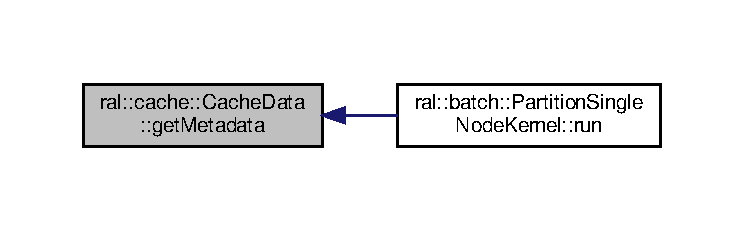
\includegraphics[width=350pt]{classral_1_1cache_1_1CacheData_a7e3fea5c3558948f4c461998f7ef434b_icgraph}
\end{center}
\end{figure}
\mbox{\Hypertarget{classral_1_1cache_1_1CacheData_aa2c8d58823d781cc1f8e6e589d897642}\label{classral_1_1cache_1_1CacheData_aa2c8d58823d781cc1f8e6e589d897642}} 
\index{ral\+::cache\+::\+Cache\+Data@{ral\+::cache\+::\+Cache\+Data}!names@{names}}
\index{names@{names}!ral\+::cache\+::\+Cache\+Data@{ral\+::cache\+::\+Cache\+Data}}
\subsubsection{\texorpdfstring{names()}{names()}}
{\footnotesize\ttfamily std\+::vector$<$std\+::string$>$ ral\+::cache\+::\+Cache\+Data\+::names (\begin{DoxyParamCaption}{ }\end{DoxyParamCaption}) const\hspace{0.3cm}{\ttfamily [inline]}}

Get the names of the columns. \begin{DoxyReturn}{Returns}
a vector of the column names 
\end{DoxyReturn}
Here is the caller graph for this function\+:\nopagebreak
\begin{figure}[H]
\begin{center}
\leavevmode
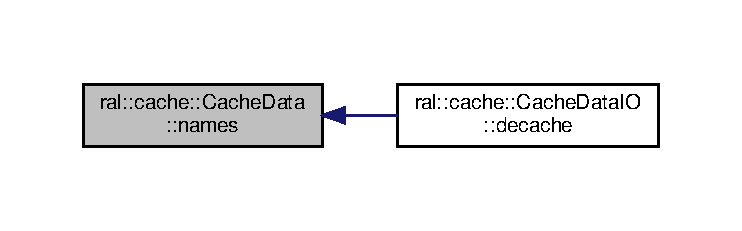
\includegraphics[width=350pt]{classral_1_1cache_1_1CacheData_aa2c8d58823d781cc1f8e6e589d897642_icgraph}
\end{center}
\end{figure}
\mbox{\Hypertarget{classral_1_1cache_1_1CacheData_acddfe8617004fc875fff972ae5b1f616}\label{classral_1_1cache_1_1CacheData_acddfe8617004fc875fff972ae5b1f616}} 
\index{ral\+::cache\+::\+Cache\+Data@{ral\+::cache\+::\+Cache\+Data}!num\+\_\+columns@{num\+\_\+columns}}
\index{num\+\_\+columns@{num\+\_\+columns}!ral\+::cache\+::\+Cache\+Data@{ral\+::cache\+::\+Cache\+Data}}
\subsubsection{\texorpdfstring{num\+\_\+columns()}{num\_columns()}}
{\footnotesize\ttfamily size\+\_\+t ral\+::cache\+::\+Cache\+Data\+::num\+\_\+columns (\begin{DoxyParamCaption}{ }\end{DoxyParamCaption}) const\hspace{0.3cm}{\ttfamily [inline]}}

Get the number of columns this \hyperlink{classral_1_1cache_1_1CacheData}{Cache\+Data} will generate with decache. \mbox{\Hypertarget{classral_1_1cache_1_1CacheData_a14a5b9fadf872c12d633e38bb6f9f07d}\label{classral_1_1cache_1_1CacheData_a14a5b9fadf872c12d633e38bb6f9f07d}} 
\index{ral\+::cache\+::\+Cache\+Data@{ral\+::cache\+::\+Cache\+Data}!num\+\_\+rows@{num\+\_\+rows}}
\index{num\+\_\+rows@{num\+\_\+rows}!ral\+::cache\+::\+Cache\+Data@{ral\+::cache\+::\+Cache\+Data}}
\subsubsection{\texorpdfstring{num\+\_\+rows()}{num\_rows()}}
{\footnotesize\ttfamily size\+\_\+t ral\+::cache\+::\+Cache\+Data\+::num\+\_\+rows (\begin{DoxyParamCaption}{ }\end{DoxyParamCaption}) const\hspace{0.3cm}{\ttfamily [inline]}}

Get the number of rows this \hyperlink{classral_1_1cache_1_1CacheData}{Cache\+Data} will generate with decache. Here is the caller graph for this function\+:\nopagebreak
\begin{figure}[H]
\begin{center}
\leavevmode
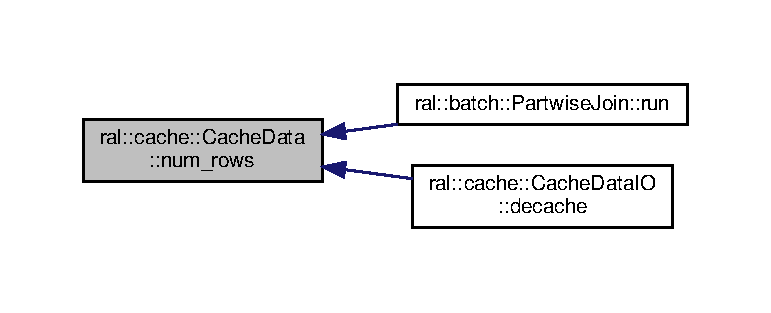
\includegraphics[width=350pt]{classral_1_1cache_1_1CacheData_a14a5b9fadf872c12d633e38bb6f9f07d_icgraph}
\end{center}
\end{figure}
\mbox{\Hypertarget{classral_1_1cache_1_1CacheData_a3bb1623a4266ba7c961d325023ff13c6}\label{classral_1_1cache_1_1CacheData_a3bb1623a4266ba7c961d325023ff13c6}} 
\index{ral\+::cache\+::\+Cache\+Data@{ral\+::cache\+::\+Cache\+Data}!set\+\_\+names@{set\+\_\+names}}
\index{set\+\_\+names@{set\+\_\+names}!ral\+::cache\+::\+Cache\+Data@{ral\+::cache\+::\+Cache\+Data}}
\subsubsection{\texorpdfstring{set\+\_\+names()}{set\_names()}}
{\footnotesize\ttfamily virtual void ral\+::cache\+::\+Cache\+Data\+::set\+\_\+names (\begin{DoxyParamCaption}\item[{const std\+::vector$<$ std\+::string $>$ \&}]{names }\end{DoxyParamCaption})\hspace{0.3cm}{\ttfamily [pure virtual]}}

Set the names of the columns. 
\begin{DoxyParams}{Parameters}
{\em names} & a vector of the column names. \\
\hline
\end{DoxyParams}


Implemented in \hyperlink{classral_1_1cache_1_1ConcatCacheData_a02f400f33f88ba3e216f5899fa4f12b8}{ral\+::cache\+::\+Concat\+Cache\+Data}, \hyperlink{classral_1_1cache_1_1CacheDataIO_a9f5ae6134a546813c74a2924f7567080}{ral\+::cache\+::\+Cache\+Data\+IO}, \hyperlink{classral_1_1cache_1_1CacheDataLocalFile_a49c8d137ef2d0a30ee59025f91725567}{ral\+::cache\+::\+Cache\+Data\+Local\+File}, \hyperlink{classral_1_1cache_1_1CPUCacheData_a3d0444ff9ba0814775499060071a2d1a}{ral\+::cache\+::\+C\+P\+U\+Cache\+Data}, and \hyperlink{classral_1_1cache_1_1GPUCacheData_a35d56396384cd4380141d47291d3e55f}{ral\+::cache\+::\+G\+P\+U\+Cache\+Data}.

\mbox{\Hypertarget{classral_1_1cache_1_1CacheData_aaad8a726296574845f01f9380dcee40d}\label{classral_1_1cache_1_1CacheData_aaad8a726296574845f01f9380dcee40d}} 
\index{ral\+::cache\+::\+Cache\+Data@{ral\+::cache\+::\+Cache\+Data}!size\+In\+Bytes@{size\+In\+Bytes}}
\index{size\+In\+Bytes@{size\+In\+Bytes}!ral\+::cache\+::\+Cache\+Data@{ral\+::cache\+::\+Cache\+Data}}
\subsubsection{\texorpdfstring{size\+In\+Bytes()}{sizeInBytes()}}
{\footnotesize\ttfamily virtual size\+\_\+t ral\+::cache\+::\+Cache\+Data\+::size\+In\+Bytes (\begin{DoxyParamCaption}{ }\end{DoxyParamCaption}) const\hspace{0.3cm}{\ttfamily [pure virtual]}}

. A pure virtual function. This removes the payload for the \hyperlink{classral_1_1cache_1_1CacheData}{Cache\+Data}. After this the \hyperlink{classral_1_1cache_1_1CacheData}{Cache\+Data} will almost always go out of scope and be destroyed. \begin{DoxyReturn}{Returns}
the number of bytes our dataframe occupies in whatever format it is being stored 
\end{DoxyReturn}


Implemented in \hyperlink{classral_1_1cache_1_1ConcatCacheData_a25914d06c36e4a1748dc9479adc5ccd8}{ral\+::cache\+::\+Concat\+Cache\+Data}, \hyperlink{classral_1_1cache_1_1CacheDataIO_a3364dc1069ceba37e2ffc97e5a4508aa}{ral\+::cache\+::\+Cache\+Data\+IO}, \hyperlink{classral_1_1cache_1_1CacheDataLocalFile_ab0853eca16df1149f4ac0efbf3faa556}{ral\+::cache\+::\+Cache\+Data\+Local\+File}, \hyperlink{classral_1_1cache_1_1CPUCacheData_a83236d09b1d2341059d1a6738839d35c}{ral\+::cache\+::\+C\+P\+U\+Cache\+Data}, and \hyperlink{classral_1_1cache_1_1GPUCacheData_a4fc8aecb334114f0ef07ce37be0e8900}{ral\+::cache\+::\+G\+P\+U\+Cache\+Data}.

Here is the caller graph for this function\+:\nopagebreak
\begin{figure}[H]
\begin{center}
\leavevmode
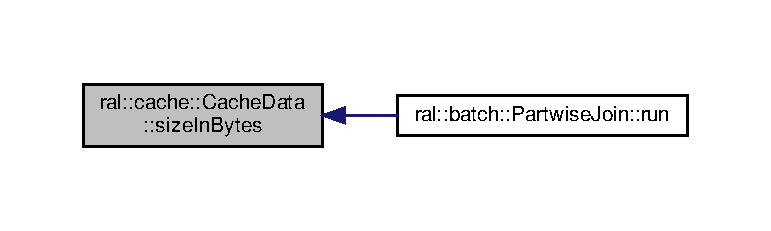
\includegraphics[width=350pt]{classral_1_1cache_1_1CacheData_aaad8a726296574845f01f9380dcee40d_icgraph}
\end{center}
\end{figure}


\subsection{Member Data Documentation}
\mbox{\Hypertarget{classral_1_1cache_1_1CacheData_acf9d130e22baac61d4689c52e36b9c17}\label{classral_1_1cache_1_1CacheData_acf9d130e22baac61d4689c52e36b9c17}} 
\index{ral\+::cache\+::\+Cache\+Data@{ral\+::cache\+::\+Cache\+Data}!cache\+\_\+type@{cache\+\_\+type}}
\index{cache\+\_\+type@{cache\+\_\+type}!ral\+::cache\+::\+Cache\+Data@{ral\+::cache\+::\+Cache\+Data}}
\subsubsection{\texorpdfstring{cache\+\_\+type}{cache\_type}}
{\footnotesize\ttfamily Cache\+Data\+Type ral\+::cache\+::\+Cache\+Data\+::cache\+\_\+type\hspace{0.3cm}{\ttfamily [protected]}}

The Cache\+Data\+Type that is used to store the dataframe representation. \mbox{\Hypertarget{classral_1_1cache_1_1CacheData_a7a43a46a362c8fe93a7af81debbeca1b}\label{classral_1_1cache_1_1CacheData_a7a43a46a362c8fe93a7af81debbeca1b}} 
\index{ral\+::cache\+::\+Cache\+Data@{ral\+::cache\+::\+Cache\+Data}!col\+\_\+names@{col\+\_\+names}}
\index{col\+\_\+names@{col\+\_\+names}!ral\+::cache\+::\+Cache\+Data@{ral\+::cache\+::\+Cache\+Data}}
\subsubsection{\texorpdfstring{col\+\_\+names}{col\_names}}
{\footnotesize\ttfamily std\+::vector$<$std\+::string$>$ ral\+::cache\+::\+Cache\+Data\+::col\+\_\+names\hspace{0.3cm}{\ttfamily [protected]}}

A vector storing the names of the columns in the dataframe representation. \mbox{\Hypertarget{classral_1_1cache_1_1CacheData_aaeb232ef3aa8c2a3d86e1169ed2e8152}\label{classral_1_1cache_1_1CacheData_aaeb232ef3aa8c2a3d86e1169ed2e8152}} 
\index{ral\+::cache\+::\+Cache\+Data@{ral\+::cache\+::\+Cache\+Data}!metadata@{metadata}}
\index{metadata@{metadata}!ral\+::cache\+::\+Cache\+Data@{ral\+::cache\+::\+Cache\+Data}}
\subsubsection{\texorpdfstring{metadata}{metadata}}
{\footnotesize\ttfamily \hyperlink{classral_1_1cache_1_1MetadataDictionary}{Metadata\+Dictionary} ral\+::cache\+::\+Cache\+Data\+::metadata\hspace{0.3cm}{\ttfamily [protected]}}

The metadata used for routing and planning. \mbox{\Hypertarget{classral_1_1cache_1_1CacheData_a4cdddfb8e552e0e3e91877ae80e5fc9e}\label{classral_1_1cache_1_1CacheData_a4cdddfb8e552e0e3e91877ae80e5fc9e}} 
\index{ral\+::cache\+::\+Cache\+Data@{ral\+::cache\+::\+Cache\+Data}!n\+\_\+rows@{n\+\_\+rows}}
\index{n\+\_\+rows@{n\+\_\+rows}!ral\+::cache\+::\+Cache\+Data@{ral\+::cache\+::\+Cache\+Data}}
\subsubsection{\texorpdfstring{n\+\_\+rows}{n\_rows}}
{\footnotesize\ttfamily size\+\_\+t ral\+::cache\+::\+Cache\+Data\+::n\+\_\+rows\hspace{0.3cm}{\ttfamily [protected]}}

Stores the number of rows in the dataframe representation. \mbox{\Hypertarget{classral_1_1cache_1_1CacheData_aec9a1b3c0fb78cfdb3bd5494bcee2d8f}\label{classral_1_1cache_1_1CacheData_aec9a1b3c0fb78cfdb3bd5494bcee2d8f}} 
\index{ral\+::cache\+::\+Cache\+Data@{ral\+::cache\+::\+Cache\+Data}!schema@{schema}}
\index{schema@{schema}!ral\+::cache\+::\+Cache\+Data@{ral\+::cache\+::\+Cache\+Data}}
\subsubsection{\texorpdfstring{schema}{schema}}
{\footnotesize\ttfamily std\+::vector$<$cudf\+::data\+\_\+type$>$ ral\+::cache\+::\+Cache\+Data\+::schema\hspace{0.3cm}{\ttfamily [protected]}}

A vector storing the cudf\+::data\+\_\+type of the columns in the dataframe representation. 

The documentation for this class was generated from the following files\+:\begin{DoxyCompactItemize}
\item 
/home/tom/\+Documents/programming/romulo\+\_\+blazingsql/blazingsql/engine/src/execution\+\_\+graph/logic\+\_\+controllers/Cache\+Data.\+h\item 
/home/tom/\+Documents/programming/romulo\+\_\+blazingsql/blazingsql/engine/src/execution\+\_\+graph/logic\+\_\+controllers/Cache\+Data.\+cpp\end{DoxyCompactItemize}

\hypertarget{classral_1_1cache_1_1CacheDataIO}{}\section{ral\+:\+:cache\+:\+:Cache\+Data\+IO Class Reference}
\label{classral_1_1cache_1_1CacheDataIO}\index{ral\+::cache\+::\+Cache\+Data\+IO@{ral\+::cache\+::\+Cache\+Data\+IO}}


{\ttfamily \#include $<$Cache\+Data.\+h$>$}



Inheritance diagram for ral\+:\+:cache\+:\+:Cache\+Data\+IO\+:\nopagebreak
\begin{figure}[H]
\begin{center}
\leavevmode
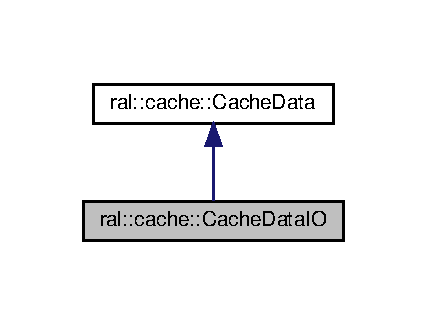
\includegraphics[width=205pt]{classral_1_1cache_1_1CacheDataIO__inherit__graph}
\end{center}
\end{figure}


Collaboration diagram for ral\+:\+:cache\+:\+:Cache\+Data\+IO\+:\nopagebreak
\begin{figure}[H]
\begin{center}
\leavevmode
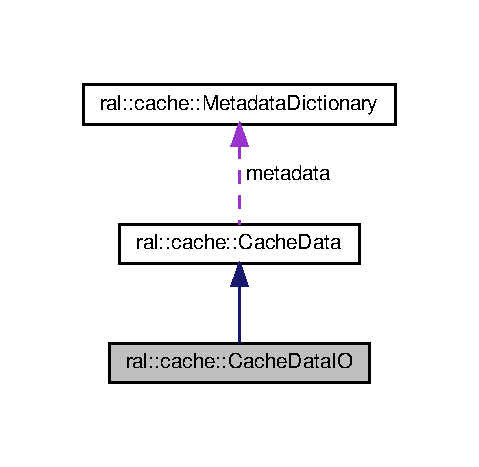
\includegraphics[width=230pt]{classral_1_1cache_1_1CacheDataIO__coll__graph}
\end{center}
\end{figure}
\subsection*{Public Member Functions}
\begin{DoxyCompactItemize}
\item 
\hyperlink{classral_1_1cache_1_1CacheDataIO_a1f6787bfd6d9555836423b6d3335ed73}{Cache\+Data\+IO} (\hyperlink{structral_1_1io_1_1data__handle}{ral\+::io\+::data\+\_\+handle} handle, std\+::shared\+\_\+ptr$<$ \hyperlink{classral_1_1io_1_1data__parser}{ral\+::io\+::data\+\_\+parser} $>$ parser, \hyperlink{classral_1_1io_1_1Schema}{ral\+::io\+::\+Schema} schema, \hyperlink{classral_1_1io_1_1Schema}{ral\+::io\+::\+Schema} file\+\_\+schema, std\+::vector$<$ int $>$ row\+\_\+group\+\_\+ids, std\+::vector$<$ int $>$ projections)
\item 
std\+::unique\+\_\+ptr$<$ \hyperlink{classral_1_1frame_1_1BlazingTable}{ral\+::frame\+::\+Blazing\+Table} $>$ \hyperlink{classral_1_1cache_1_1CacheDataIO_a7fb2dceef20a385e31508ac70edfbf58}{decache} () override
\item 
size\+\_\+t \hyperlink{classral_1_1cache_1_1CacheDataIO_a3364dc1069ceba37e2ffc97e5a4508aa}{size\+In\+Bytes} () const override
\item 
void \hyperlink{classral_1_1cache_1_1CacheDataIO_a9f5ae6134a546813c74a2924f7567080}{set\+\_\+names} (const std\+::vector$<$ std\+::string $>$ \&\hyperlink{classral_1_1cache_1_1CacheData_aa2c8d58823d781cc1f8e6e589d897642}{names}) override
\item 
virtual \hyperlink{classral_1_1cache_1_1CacheDataIO_a335ec293cd6e3d928396ae99e3785906}{$\sim$\+Cache\+Data\+IO} ()
\end{DoxyCompactItemize}
\subsection*{Additional Inherited Members}


\subsection{Detailed Description}
A \hyperlink{classral_1_1cache_1_1CacheData}{Cache\+Data} that stores is data in an O\+RC file. This allows us to cache onto filesystems to allow larger queries to run on limited resources. This is the least performant cache in most instances. 

\subsection{Constructor \& Destructor Documentation}
\mbox{\Hypertarget{classral_1_1cache_1_1CacheDataIO_a1f6787bfd6d9555836423b6d3335ed73}\label{classral_1_1cache_1_1CacheDataIO_a1f6787bfd6d9555836423b6d3335ed73}} 
\index{ral\+::cache\+::\+Cache\+Data\+IO@{ral\+::cache\+::\+Cache\+Data\+IO}!Cache\+Data\+IO@{Cache\+Data\+IO}}
\index{Cache\+Data\+IO@{Cache\+Data\+IO}!ral\+::cache\+::\+Cache\+Data\+IO@{ral\+::cache\+::\+Cache\+Data\+IO}}
\subsubsection{\texorpdfstring{Cache\+Data\+I\+O()}{CacheDataIO()}}
{\footnotesize\ttfamily ral\+::cache\+::\+Cache\+Data\+I\+O\+::\+Cache\+Data\+IO (\begin{DoxyParamCaption}\item[{\hyperlink{structral_1_1io_1_1data__handle}{ral\+::io\+::data\+\_\+handle}}]{handle,  }\item[{std\+::shared\+\_\+ptr$<$ \hyperlink{classral_1_1io_1_1data__parser}{ral\+::io\+::data\+\_\+parser} $>$}]{parser,  }\item[{\hyperlink{classral_1_1io_1_1Schema}{ral\+::io\+::\+Schema}}]{schema,  }\item[{\hyperlink{classral_1_1io_1_1Schema}{ral\+::io\+::\+Schema}}]{file\+\_\+schema,  }\item[{std\+::vector$<$ int $>$}]{row\+\_\+group\+\_\+ids,  }\item[{std\+::vector$<$ int $>$}]{projections }\end{DoxyParamCaption})}

Constructor 
\begin{DoxyParams}{Parameters}
{\em table} & The Blazing\+Table that is converted into an O\+RC file and stored on disk. @ param orc\+\_\+files\+\_\+path The path where the file should be stored. \\
\hline
\end{DoxyParams}
\mbox{\Hypertarget{classral_1_1cache_1_1CacheDataIO_a335ec293cd6e3d928396ae99e3785906}\label{classral_1_1cache_1_1CacheDataIO_a335ec293cd6e3d928396ae99e3785906}} 
\index{ral\+::cache\+::\+Cache\+Data\+IO@{ral\+::cache\+::\+Cache\+Data\+IO}!````~Cache\+Data\+IO@{$\sim$\+Cache\+Data\+IO}}
\index{````~Cache\+Data\+IO@{$\sim$\+Cache\+Data\+IO}!ral\+::cache\+::\+Cache\+Data\+IO@{ral\+::cache\+::\+Cache\+Data\+IO}}
\subsubsection{\texorpdfstring{$\sim$\+Cache\+Data\+I\+O()}{~CacheDataIO()}}
{\footnotesize\ttfamily virtual ral\+::cache\+::\+Cache\+Data\+I\+O\+::$\sim$\+Cache\+Data\+IO (\begin{DoxyParamCaption}{ }\end{DoxyParamCaption})\hspace{0.3cm}{\ttfamily [inline]}, {\ttfamily [virtual]}}

Destructor 

\subsection{Member Function Documentation}
\mbox{\Hypertarget{classral_1_1cache_1_1CacheDataIO_a7fb2dceef20a385e31508ac70edfbf58}\label{classral_1_1cache_1_1CacheDataIO_a7fb2dceef20a385e31508ac70edfbf58}} 
\index{ral\+::cache\+::\+Cache\+Data\+IO@{ral\+::cache\+::\+Cache\+Data\+IO}!decache@{decache}}
\index{decache@{decache}!ral\+::cache\+::\+Cache\+Data\+IO@{ral\+::cache\+::\+Cache\+Data\+IO}}
\subsubsection{\texorpdfstring{decache()}{decache()}}
{\footnotesize\ttfamily std\+::unique\+\_\+ptr$<$ \hyperlink{classral_1_1frame_1_1BlazingTable}{ral\+::frame\+::\+Blazing\+Table} $>$ ral\+::cache\+::\+Cache\+Data\+I\+O\+::decache (\begin{DoxyParamCaption}{ }\end{DoxyParamCaption})\hspace{0.3cm}{\ttfamily [override]}, {\ttfamily [virtual]}}

Constructor 
\begin{DoxyParams}{Parameters}
{\em table} & The Blazing\+Table that is converted into an O\+RC file and stored on disk. @ param orc\+\_\+files\+\_\+path The path where the file should be stored. \\
\hline
\end{DoxyParams}


Implements \hyperlink{classral_1_1cache_1_1CacheData_a2db8fdd2151babd7a07f4c6e246b710c}{ral\+::cache\+::\+Cache\+Data}.

Here is the call graph for this function\+:\nopagebreak
\begin{figure}[H]
\begin{center}
\leavevmode
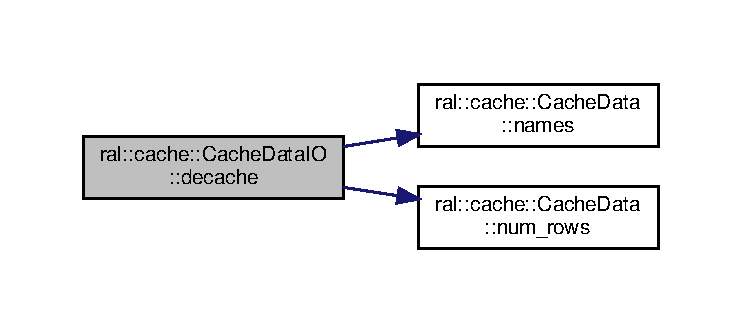
\includegraphics[width=350pt]{classral_1_1cache_1_1CacheDataIO_a7fb2dceef20a385e31508ac70edfbf58_cgraph}
\end{center}
\end{figure}
\mbox{\Hypertarget{classral_1_1cache_1_1CacheDataIO_a9f5ae6134a546813c74a2924f7567080}\label{classral_1_1cache_1_1CacheDataIO_a9f5ae6134a546813c74a2924f7567080}} 
\index{ral\+::cache\+::\+Cache\+Data\+IO@{ral\+::cache\+::\+Cache\+Data\+IO}!set\+\_\+names@{set\+\_\+names}}
\index{set\+\_\+names@{set\+\_\+names}!ral\+::cache\+::\+Cache\+Data\+IO@{ral\+::cache\+::\+Cache\+Data\+IO}}
\subsubsection{\texorpdfstring{set\+\_\+names()}{set\_names()}}
{\footnotesize\ttfamily void ral\+::cache\+::\+Cache\+Data\+I\+O\+::set\+\_\+names (\begin{DoxyParamCaption}\item[{const std\+::vector$<$ std\+::string $>$ \&}]{names }\end{DoxyParamCaption})\hspace{0.3cm}{\ttfamily [inline]}, {\ttfamily [override]}, {\ttfamily [virtual]}}

Set the names of the columns from the schema. 
\begin{DoxyParams}{Parameters}
{\em names} & a vector of the column names. \\
\hline
\end{DoxyParams}


Implements \hyperlink{classral_1_1cache_1_1CacheData_a3bb1623a4266ba7c961d325023ff13c6}{ral\+::cache\+::\+Cache\+Data}.

\mbox{\Hypertarget{classral_1_1cache_1_1CacheDataIO_a3364dc1069ceba37e2ffc97e5a4508aa}\label{classral_1_1cache_1_1CacheDataIO_a3364dc1069ceba37e2ffc97e5a4508aa}} 
\index{ral\+::cache\+::\+Cache\+Data\+IO@{ral\+::cache\+::\+Cache\+Data\+IO}!size\+In\+Bytes@{size\+In\+Bytes}}
\index{size\+In\+Bytes@{size\+In\+Bytes}!ral\+::cache\+::\+Cache\+Data\+IO@{ral\+::cache\+::\+Cache\+Data\+IO}}
\subsubsection{\texorpdfstring{size\+In\+Bytes()}{sizeInBytes()}}
{\footnotesize\ttfamily size\+\_\+t ral\+::cache\+::\+Cache\+Data\+I\+O\+::size\+In\+Bytes (\begin{DoxyParamCaption}{ }\end{DoxyParamCaption}) const\hspace{0.3cm}{\ttfamily [override]}, {\ttfamily [virtual]}}

Get the amount of G\+PU memory that the decached Blazing\+Table W\+O\+U\+LD consume. Having this function allows us to have one api for seeing how much G\+PU memory is necessary to decache the file from disk. \begin{DoxyReturn}{Returns}
The number of bytes needed for the Blazing\+Table decache would generate. 
\end{DoxyReturn}


Implements \hyperlink{classral_1_1cache_1_1CacheData_aaad8a726296574845f01f9380dcee40d}{ral\+::cache\+::\+Cache\+Data}.



The documentation for this class was generated from the following files\+:\begin{DoxyCompactItemize}
\item 
/home/tom/\+Documents/programming/romulo\+\_\+blazingsql/blazingsql/engine/src/execution\+\_\+graph/logic\+\_\+controllers/Cache\+Data.\+h\item 
/home/tom/\+Documents/programming/romulo\+\_\+blazingsql/blazingsql/engine/src/execution\+\_\+graph/logic\+\_\+controllers/Cache\+Data.\+cpp\end{DoxyCompactItemize}

\hypertarget{classral_1_1cache_1_1CacheDataLocalFile}{}\section{ral\+:\+:cache\+:\+:Cache\+Data\+Local\+File Class Reference}
\label{classral_1_1cache_1_1CacheDataLocalFile}\index{ral\+::cache\+::\+Cache\+Data\+Local\+File@{ral\+::cache\+::\+Cache\+Data\+Local\+File}}


{\ttfamily \#include $<$Cache\+Data.\+h$>$}



Inheritance diagram for ral\+:\+:cache\+:\+:Cache\+Data\+Local\+File\+:\nopagebreak
\begin{figure}[H]
\begin{center}
\leavevmode
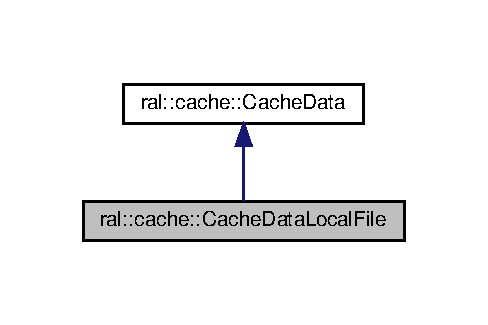
\includegraphics[width=234pt]{classral_1_1cache_1_1CacheDataLocalFile__inherit__graph}
\end{center}
\end{figure}


Collaboration diagram for ral\+:\+:cache\+:\+:Cache\+Data\+Local\+File\+:\nopagebreak
\begin{figure}[H]
\begin{center}
\leavevmode
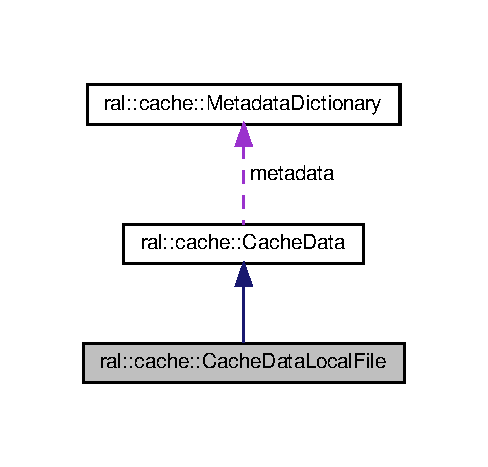
\includegraphics[width=234pt]{classral_1_1cache_1_1CacheDataLocalFile__coll__graph}
\end{center}
\end{figure}
\subsection*{Public Member Functions}
\begin{DoxyCompactItemize}
\item 
\hyperlink{classral_1_1cache_1_1CacheDataLocalFile_aa8f42a81e963c076ebdf7bc6bc53a323}{Cache\+Data\+Local\+File} (std\+::unique\+\_\+ptr$<$ \hyperlink{classral_1_1frame_1_1BlazingTable}{ral\+::frame\+::\+Blazing\+Table} $>$ table, std\+::string orc\+\_\+files\+\_\+path, std\+::string ctx\+\_\+token)
\item 
std\+::unique\+\_\+ptr$<$ \hyperlink{classral_1_1frame_1_1BlazingTable}{ral\+::frame\+::\+Blazing\+Table} $>$ \hyperlink{classral_1_1cache_1_1CacheDataLocalFile_a1d34227fbbf671e47119846ee2f2a0af}{decache} () override
\item 
size\+\_\+t \hyperlink{classral_1_1cache_1_1CacheDataLocalFile_ab0853eca16df1149f4ac0efbf3faa556}{size\+In\+Bytes} () const override
\item 
size\+\_\+t \hyperlink{classral_1_1cache_1_1CacheDataLocalFile_abc8a4d9edc7ffa21f15010c60a71189b}{file\+Size\+In\+Bytes} () const
\item 
void \hyperlink{classral_1_1cache_1_1CacheDataLocalFile_a49c8d137ef2d0a30ee59025f91725567}{set\+\_\+names} (const std\+::vector$<$ std\+::string $>$ \&\hyperlink{classral_1_1cache_1_1CacheData_aa2c8d58823d781cc1f8e6e589d897642}{names}) override
\item 
virtual \hyperlink{classral_1_1cache_1_1CacheDataLocalFile_a47567f8650eae4b66e44df7e06f3def9}{$\sim$\+Cache\+Data\+Local\+File} ()
\item 
std\+::string \hyperlink{classral_1_1cache_1_1CacheDataLocalFile_a21803499ee4d3ad088c2b5b81b91a042}{file\+Path} () const
\end{DoxyCompactItemize}
\subsection*{Additional Inherited Members}


\subsection{Detailed Description}
A \hyperlink{classral_1_1cache_1_1CacheData}{Cache\+Data} that stores is data in an O\+RC file. This allows us to cache onto filesystems to allow larger queries to run on limited resources. This is the least performant cache in most instances. 

\subsection{Constructor \& Destructor Documentation}
\mbox{\Hypertarget{classral_1_1cache_1_1CacheDataLocalFile_aa8f42a81e963c076ebdf7bc6bc53a323}\label{classral_1_1cache_1_1CacheDataLocalFile_aa8f42a81e963c076ebdf7bc6bc53a323}} 
\index{ral\+::cache\+::\+Cache\+Data\+Local\+File@{ral\+::cache\+::\+Cache\+Data\+Local\+File}!Cache\+Data\+Local\+File@{Cache\+Data\+Local\+File}}
\index{Cache\+Data\+Local\+File@{Cache\+Data\+Local\+File}!ral\+::cache\+::\+Cache\+Data\+Local\+File@{ral\+::cache\+::\+Cache\+Data\+Local\+File}}
\subsubsection{\texorpdfstring{Cache\+Data\+Local\+File()}{CacheDataLocalFile()}}
{\footnotesize\ttfamily ral\+::cache\+::\+Cache\+Data\+Local\+File\+::\+Cache\+Data\+Local\+File (\begin{DoxyParamCaption}\item[{std\+::unique\+\_\+ptr$<$ \hyperlink{classral_1_1frame_1_1BlazingTable}{ral\+::frame\+::\+Blazing\+Table} $>$}]{table,  }\item[{std\+::string}]{orc\+\_\+files\+\_\+path,  }\item[{std\+::string}]{ctx\+\_\+token }\end{DoxyParamCaption})}

Constructor 
\begin{DoxyParams}{Parameters}
{\em table} & The Blazing\+Table that is converted into an O\+RC file and stored on disk. @ param orc\+\_\+files\+\_\+path The path where the file should be stored. @ param ctx\+\_\+id The context token to identify the query that generated the file. \\
\hline
\end{DoxyParams}
\mbox{\Hypertarget{classral_1_1cache_1_1CacheDataLocalFile_a47567f8650eae4b66e44df7e06f3def9}\label{classral_1_1cache_1_1CacheDataLocalFile_a47567f8650eae4b66e44df7e06f3def9}} 
\index{ral\+::cache\+::\+Cache\+Data\+Local\+File@{ral\+::cache\+::\+Cache\+Data\+Local\+File}!````~Cache\+Data\+Local\+File@{$\sim$\+Cache\+Data\+Local\+File}}
\index{````~Cache\+Data\+Local\+File@{$\sim$\+Cache\+Data\+Local\+File}!ral\+::cache\+::\+Cache\+Data\+Local\+File@{ral\+::cache\+::\+Cache\+Data\+Local\+File}}
\subsubsection{\texorpdfstring{$\sim$\+Cache\+Data\+Local\+File()}{~CacheDataLocalFile()}}
{\footnotesize\ttfamily virtual ral\+::cache\+::\+Cache\+Data\+Local\+File\+::$\sim$\+Cache\+Data\+Local\+File (\begin{DoxyParamCaption}{ }\end{DoxyParamCaption})\hspace{0.3cm}{\ttfamily [inline]}, {\ttfamily [virtual]}}

Destructor 

\subsection{Member Function Documentation}
\mbox{\Hypertarget{classral_1_1cache_1_1CacheDataLocalFile_a1d34227fbbf671e47119846ee2f2a0af}\label{classral_1_1cache_1_1CacheDataLocalFile_a1d34227fbbf671e47119846ee2f2a0af}} 
\index{ral\+::cache\+::\+Cache\+Data\+Local\+File@{ral\+::cache\+::\+Cache\+Data\+Local\+File}!decache@{decache}}
\index{decache@{decache}!ral\+::cache\+::\+Cache\+Data\+Local\+File@{ral\+::cache\+::\+Cache\+Data\+Local\+File}}
\subsubsection{\texorpdfstring{decache()}{decache()}}
{\footnotesize\ttfamily std\+::unique\+\_\+ptr$<$ \hyperlink{classral_1_1frame_1_1BlazingTable}{ral\+::frame\+::\+Blazing\+Table} $>$ ral\+::cache\+::\+Cache\+Data\+Local\+File\+::decache (\begin{DoxyParamCaption}{ }\end{DoxyParamCaption})\hspace{0.3cm}{\ttfamily [override]}, {\ttfamily [virtual]}}

Constructor 
\begin{DoxyParams}{Parameters}
{\em table} & The Blazing\+Table that is converted into an O\+RC file and stored on disk. @ param orc\+\_\+files\+\_\+path The path where the file should be stored. \\
\hline
\end{DoxyParams}


Implements \hyperlink{classral_1_1cache_1_1CacheData_a2db8fdd2151babd7a07f4c6e246b710c}{ral\+::cache\+::\+Cache\+Data}.

\mbox{\Hypertarget{classral_1_1cache_1_1CacheDataLocalFile_a21803499ee4d3ad088c2b5b81b91a042}\label{classral_1_1cache_1_1CacheDataLocalFile_a21803499ee4d3ad088c2b5b81b91a042}} 
\index{ral\+::cache\+::\+Cache\+Data\+Local\+File@{ral\+::cache\+::\+Cache\+Data\+Local\+File}!file\+Path@{file\+Path}}
\index{file\+Path@{file\+Path}!ral\+::cache\+::\+Cache\+Data\+Local\+File@{ral\+::cache\+::\+Cache\+Data\+Local\+File}}
\subsubsection{\texorpdfstring{file\+Path()}{filePath()}}
{\footnotesize\ttfamily std\+::string ral\+::cache\+::\+Cache\+Data\+Local\+File\+::file\+Path (\begin{DoxyParamCaption}{ }\end{DoxyParamCaption}) const\hspace{0.3cm}{\ttfamily [inline]}}

Get the file path of the O\+RC file. \begin{DoxyReturn}{Returns}
The path to the O\+RC file. 
\end{DoxyReturn}
\mbox{\Hypertarget{classral_1_1cache_1_1CacheDataLocalFile_abc8a4d9edc7ffa21f15010c60a71189b}\label{classral_1_1cache_1_1CacheDataLocalFile_abc8a4d9edc7ffa21f15010c60a71189b}} 
\index{ral\+::cache\+::\+Cache\+Data\+Local\+File@{ral\+::cache\+::\+Cache\+Data\+Local\+File}!file\+Size\+In\+Bytes@{file\+Size\+In\+Bytes}}
\index{file\+Size\+In\+Bytes@{file\+Size\+In\+Bytes}!ral\+::cache\+::\+Cache\+Data\+Local\+File@{ral\+::cache\+::\+Cache\+Data\+Local\+File}}
\subsubsection{\texorpdfstring{file\+Size\+In\+Bytes()}{fileSizeInBytes()}}
{\footnotesize\ttfamily size\+\_\+t ral\+::cache\+::\+Cache\+Data\+Local\+File\+::file\+Size\+In\+Bytes (\begin{DoxyParamCaption}{ }\end{DoxyParamCaption}) const}

Get the amount of disk space consumed by this \hyperlink{classral_1_1cache_1_1CacheData}{Cache\+Data} Having this function allows us to have one api for seeing the consumption of all the \hyperlink{classral_1_1cache_1_1CacheData}{Cache\+Data} objects that are currently in Caches. \begin{DoxyReturn}{Returns}
The number of bytes the O\+RC file consumes. 
\end{DoxyReturn}
\mbox{\Hypertarget{classral_1_1cache_1_1CacheDataLocalFile_a49c8d137ef2d0a30ee59025f91725567}\label{classral_1_1cache_1_1CacheDataLocalFile_a49c8d137ef2d0a30ee59025f91725567}} 
\index{ral\+::cache\+::\+Cache\+Data\+Local\+File@{ral\+::cache\+::\+Cache\+Data\+Local\+File}!set\+\_\+names@{set\+\_\+names}}
\index{set\+\_\+names@{set\+\_\+names}!ral\+::cache\+::\+Cache\+Data\+Local\+File@{ral\+::cache\+::\+Cache\+Data\+Local\+File}}
\subsubsection{\texorpdfstring{set\+\_\+names()}{set\_names()}}
{\footnotesize\ttfamily void ral\+::cache\+::\+Cache\+Data\+Local\+File\+::set\+\_\+names (\begin{DoxyParamCaption}\item[{const std\+::vector$<$ std\+::string $>$ \&}]{names }\end{DoxyParamCaption})\hspace{0.3cm}{\ttfamily [inline]}, {\ttfamily [override]}, {\ttfamily [virtual]}}

Set the names of the columns to pass when decache if needed. 
\begin{DoxyParams}{Parameters}
{\em names} & a vector of the column names. \\
\hline
\end{DoxyParams}


Implements \hyperlink{classral_1_1cache_1_1CacheData_a3bb1623a4266ba7c961d325023ff13c6}{ral\+::cache\+::\+Cache\+Data}.

\mbox{\Hypertarget{classral_1_1cache_1_1CacheDataLocalFile_ab0853eca16df1149f4ac0efbf3faa556}\label{classral_1_1cache_1_1CacheDataLocalFile_ab0853eca16df1149f4ac0efbf3faa556}} 
\index{ral\+::cache\+::\+Cache\+Data\+Local\+File@{ral\+::cache\+::\+Cache\+Data\+Local\+File}!size\+In\+Bytes@{size\+In\+Bytes}}
\index{size\+In\+Bytes@{size\+In\+Bytes}!ral\+::cache\+::\+Cache\+Data\+Local\+File@{ral\+::cache\+::\+Cache\+Data\+Local\+File}}
\subsubsection{\texorpdfstring{size\+In\+Bytes()}{sizeInBytes()}}
{\footnotesize\ttfamily size\+\_\+t ral\+::cache\+::\+Cache\+Data\+Local\+File\+::size\+In\+Bytes (\begin{DoxyParamCaption}{ }\end{DoxyParamCaption}) const\hspace{0.3cm}{\ttfamily [override]}, {\ttfamily [virtual]}}

Get the amount of G\+PU memory that the decached Blazing\+Table W\+O\+U\+LD consume. Having this function allows us to have one api for seeing how much G\+PU memory is necessary to decache the file from disk. \begin{DoxyReturn}{Returns}
The number of bytes needed for the Blazing\+Table decache would generate. 
\end{DoxyReturn}


Implements \hyperlink{classral_1_1cache_1_1CacheData_aaad8a726296574845f01f9380dcee40d}{ral\+::cache\+::\+Cache\+Data}.



The documentation for this class was generated from the following files\+:\begin{DoxyCompactItemize}
\item 
/home/tom/\+Documents/programming/romulo\+\_\+blazingsql/blazingsql/engine/src/execution\+\_\+graph/logic\+\_\+controllers/Cache\+Data.\+h\item 
/home/tom/\+Documents/programming/romulo\+\_\+blazingsql/blazingsql/engine/src/execution\+\_\+graph/logic\+\_\+controllers/Cache\+Data.\+cpp\end{DoxyCompactItemize}

\hypertarget{classral_1_1cache_1_1CacheMachine}{}\section{ral\+:\+:cache\+:\+:Cache\+Machine Class Reference}
\label{classral_1_1cache_1_1CacheMachine}\index{ral\+::cache\+::\+Cache\+Machine@{ral\+::cache\+::\+Cache\+Machine}}


A class that represents a Cache Machine on a multi-\/tier (G\+PU memory, C\+PU memory, Disk memory) cache system.  




{\ttfamily \#include $<$Cache\+Machine.\+h$>$}



Inheritance diagram for ral\+:\+:cache\+:\+:Cache\+Machine\+:\nopagebreak
\begin{figure}[H]
\begin{center}
\leavevmode
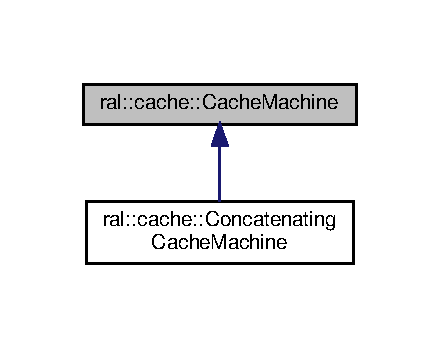
\includegraphics[width=211pt]{classral_1_1cache_1_1CacheMachine__inherit__graph}
\end{center}
\end{figure}
\subsection*{Public Member Functions}
\begin{DoxyCompactItemize}
\item 
\mbox{\Hypertarget{classral_1_1cache_1_1CacheMachine_a56079d9ace98b5755643a9f9d6f05e88}\label{classral_1_1cache_1_1CacheMachine_a56079d9ace98b5755643a9f9d6f05e88}} 
{\bfseries Cache\+Machine} (std\+::shared\+\_\+ptr$<$ \hyperlink{classblazingdb_1_1manager_1_1Context}{Context} $>$ context, std\+::string cache\+\_\+machine\+\_\+name, bool log\+\_\+timeout=true, int cache\+\_\+level\+\_\+override=-\/1, bool is\+\_\+array\+\_\+access=false)
\item 
\mbox{\Hypertarget{classral_1_1cache_1_1CacheMachine_a27088fefa2a1edcf5729e2df01043d49}\label{classral_1_1cache_1_1CacheMachine_a27088fefa2a1edcf5729e2df01043d49}} 
virtual void {\bfseries put} (size\+\_\+t index, std\+::unique\+\_\+ptr$<$ \hyperlink{classral_1_1frame_1_1BlazingTable}{ral\+::frame\+::\+Blazing\+Table} $>$ table)
\item 
\mbox{\Hypertarget{classral_1_1cache_1_1CacheMachine_aaaef8954262a3745d30087550120fe6f}\label{classral_1_1cache_1_1CacheMachine_aaaef8954262a3745d30087550120fe6f}} 
virtual std\+::unique\+\_\+ptr$<$ \hyperlink{classral_1_1frame_1_1BlazingTable}{ral\+::frame\+::\+Blazing\+Table} $>$ {\bfseries get\+\_\+or\+\_\+wait} (size\+\_\+t index)
\item 
\mbox{\Hypertarget{classral_1_1cache_1_1CacheMachine_ab6b8f6d16284a9fe0ced6fe8c22be4f0}\label{classral_1_1cache_1_1CacheMachine_ab6b8f6d16284a9fe0ced6fe8c22be4f0}} 
virtual std\+::unique\+\_\+ptr$<$ \hyperlink{classral_1_1cache_1_1CacheData}{ral\+::cache\+::\+Cache\+Data} $>$ {\bfseries get\+\_\+or\+\_\+wait\+\_\+\+Cache\+Data} (size\+\_\+t index)
\item 
\mbox{\Hypertarget{classral_1_1cache_1_1CacheMachine_ac8279867d62662b93eb1649257e943a4}\label{classral_1_1cache_1_1CacheMachine_ac8279867d62662b93eb1649257e943a4}} 
virtual void {\bfseries clear} ()
\item 
\mbox{\Hypertarget{classral_1_1cache_1_1CacheMachine_a85a26fe9c3ea4139fce1f6cd0fc6513c}\label{classral_1_1cache_1_1CacheMachine_a85a26fe9c3ea4139fce1f6cd0fc6513c}} 
virtual bool {\bfseries add\+To\+Cache} (std\+::unique\+\_\+ptr$<$ \hyperlink{classral_1_1frame_1_1BlazingTable}{ral\+::frame\+::\+Blazing\+Table} $>$ table, std\+::string message\+\_\+id=\char`\"{}\char`\"{}, bool always\+\_\+add=false, const \hyperlink{classral_1_1cache_1_1MetadataDictionary}{Metadata\+Dictionary} \&metadata=\{\}, bool include\+\_\+meta=false, bool use\+\_\+pinned=false)
\item 
\mbox{\Hypertarget{classral_1_1cache_1_1CacheMachine_abfda7b34f09919f0d6e787f7e60c6f5f}\label{classral_1_1cache_1_1CacheMachine_abfda7b34f09919f0d6e787f7e60c6f5f}} 
virtual bool {\bfseries add\+Cache\+Data} (std\+::unique\+\_\+ptr$<$ \hyperlink{classral_1_1cache_1_1CacheData}{ral\+::cache\+::\+Cache\+Data} $>$ cache\+\_\+data, std\+::string message\+\_\+id=\char`\"{}\char`\"{}, bool always\+\_\+add=false)
\item 
\mbox{\Hypertarget{classral_1_1cache_1_1CacheMachine_a3e8733825ff2953c131b7fd3abd07e3f}\label{classral_1_1cache_1_1CacheMachine_a3e8733825ff2953c131b7fd3abd07e3f}} 
virtual bool {\bfseries add\+Host\+Frame\+To\+Cache} (std\+::unique\+\_\+ptr$<$ \hyperlink{classral_1_1frame_1_1BlazingHostTable}{ral\+::frame\+::\+Blazing\+Host\+Table} $>$ table, std\+::string message\+\_\+id=\char`\"{}\char`\"{})
\item 
\mbox{\Hypertarget{classral_1_1cache_1_1CacheMachine_aab478de640f49d2fa11ba204f102153a}\label{classral_1_1cache_1_1CacheMachine_aab478de640f49d2fa11ba204f102153a}} 
virtual void {\bfseries finish} ()
\item 
\mbox{\Hypertarget{classral_1_1cache_1_1CacheMachine_a4d319a36a1b4144b6325d3d82786b7ef}\label{classral_1_1cache_1_1CacheMachine_a4d319a36a1b4144b6325d3d82786b7ef}} 
virtual bool {\bfseries is\+\_\+finished} ()
\item 
\mbox{\Hypertarget{classral_1_1cache_1_1CacheMachine_ab0f88af62cb603f08cda0586bdab5103}\label{classral_1_1cache_1_1CacheMachine_ab0f88af62cb603f08cda0586bdab5103}} 
uint64\+\_\+t {\bfseries get\+\_\+num\+\_\+bytes\+\_\+added} ()
\item 
\mbox{\Hypertarget{classral_1_1cache_1_1CacheMachine_aa6615e5845b771141193fac07dfa995d}\label{classral_1_1cache_1_1CacheMachine_aa6615e5845b771141193fac07dfa995d}} 
uint64\+\_\+t {\bfseries get\+\_\+num\+\_\+rows\+\_\+added} ()
\item 
\mbox{\Hypertarget{classral_1_1cache_1_1CacheMachine_aabae7b958940395ee04d563f33a58dcf}\label{classral_1_1cache_1_1CacheMachine_aabae7b958940395ee04d563f33a58dcf}} 
uint64\+\_\+t {\bfseries get\+\_\+num\+\_\+batches\+\_\+added} ()
\item 
\mbox{\Hypertarget{classral_1_1cache_1_1CacheMachine_a6d6fc8c2a2ae96c3d22b2a78baf8baf8}\label{classral_1_1cache_1_1CacheMachine_a6d6fc8c2a2ae96c3d22b2a78baf8baf8}} 
void {\bfseries wait\+\_\+until\+\_\+finished} ()
\item 
\mbox{\Hypertarget{classral_1_1cache_1_1CacheMachine_a212df32ccc0efca1acec0b2030ee195e}\label{classral_1_1cache_1_1CacheMachine_a212df32ccc0efca1acec0b2030ee195e}} 
std\+::int32\+\_\+t {\bfseries get\+\_\+id} () const
\item 
\mbox{\Hypertarget{classral_1_1cache_1_1CacheMachine_a015581f7d6250f93a467f0c31f3cff78}\label{classral_1_1cache_1_1CacheMachine_a015581f7d6250f93a467f0c31f3cff78}} 
\hyperlink{classblazingdb_1_1manager_1_1Context}{Context} $\ast$ {\bfseries get\+\_\+context} () const
\item 
\mbox{\Hypertarget{classral_1_1cache_1_1CacheMachine_a0f2849bf7c9d8b32f66a811cae4e78b3}\label{classral_1_1cache_1_1CacheMachine_a0f2849bf7c9d8b32f66a811cae4e78b3}} 
bool {\bfseries wait\+\_\+for\+\_\+next} ()
\item 
\mbox{\Hypertarget{classral_1_1cache_1_1CacheMachine_ac1b8751e117b03c5f139f84958047a70}\label{classral_1_1cache_1_1CacheMachine_ac1b8751e117b03c5f139f84958047a70}} 
bool {\bfseries has\+\_\+next\+\_\+now} ()
\item 
\mbox{\Hypertarget{classral_1_1cache_1_1CacheMachine_a0a1c9eec7f235b501fa7c89724c17bc3}\label{classral_1_1cache_1_1CacheMachine_a0a1c9eec7f235b501fa7c89724c17bc3}} 
bool {\bfseries has\+\_\+messages\+\_\+now} (std\+::vector$<$ std\+::string $>$ messages)
\item 
\mbox{\Hypertarget{classral_1_1cache_1_1CacheMachine_abc6a926c6a31b4733c0c6c0f47e4683d}\label{classral_1_1cache_1_1CacheMachine_abc6a926c6a31b4733c0c6c0f47e4683d}} 
std\+::size\+\_\+t {\bfseries get\+\_\+num\+\_\+batches} ()
\item 
\mbox{\Hypertarget{classral_1_1cache_1_1CacheMachine_ab3e6a40003af362a3f35b07ac7621659}\label{classral_1_1cache_1_1CacheMachine_ab3e6a40003af362a3f35b07ac7621659}} 
virtual std\+::unique\+\_\+ptr$<$ \hyperlink{classral_1_1frame_1_1BlazingTable}{ral\+::frame\+::\+Blazing\+Table} $>$ {\bfseries pull\+From\+Cache} ()
\item 
\mbox{\Hypertarget{classral_1_1cache_1_1CacheMachine_a6231339e90316bef6e87a0956276da90}\label{classral_1_1cache_1_1CacheMachine_a6231339e90316bef6e87a0956276da90}} 
virtual std\+::unique\+\_\+ptr$<$ \hyperlink{classral_1_1frame_1_1BlazingTable}{ral\+::frame\+::\+Blazing\+Table} $>$ {\bfseries pull\+Unordered\+From\+Cache} ()
\item 
\mbox{\Hypertarget{classral_1_1cache_1_1CacheMachine_a0f021fd997c60f3c25bf865e3e4b21e6}\label{classral_1_1cache_1_1CacheMachine_a0f021fd997c60f3c25bf865e3e4b21e6}} 
std\+::vector$<$ std\+::unique\+\_\+ptr$<$ \hyperlink{classral_1_1cache_1_1CacheData}{ral\+::cache\+::\+Cache\+Data} $>$ $>$ {\bfseries pull\+\_\+all\+\_\+cache\+\_\+data} ()
\item 
\mbox{\Hypertarget{classral_1_1cache_1_1CacheMachine_a6acb39f2e7d87ea70e6bd1f51fc48bfe}\label{classral_1_1cache_1_1CacheMachine_a6acb39f2e7d87ea70e6bd1f51fc48bfe}} 
virtual std\+::unique\+\_\+ptr$<$ \hyperlink{classral_1_1cache_1_1CacheData}{ral\+::cache\+::\+Cache\+Data} $>$ {\bfseries pull\+Cache\+Data} (std\+::string message\+\_\+id)
\item 
\mbox{\Hypertarget{classral_1_1cache_1_1CacheMachine_a64c08602e07aa3643c38b43672df1907}\label{classral_1_1cache_1_1CacheMachine_a64c08602e07aa3643c38b43672df1907}} 
virtual std\+::unique\+\_\+ptr$<$ \hyperlink{classral_1_1cache_1_1CacheData}{ral\+::cache\+::\+Cache\+Data} $>$ {\bfseries pull\+Cache\+Data} ()
\item 
\mbox{\Hypertarget{classral_1_1cache_1_1CacheMachine_a0f16ba71e498e556dd34d48f21228298}\label{classral_1_1cache_1_1CacheMachine_a0f16ba71e498e556dd34d48f21228298}} 
std\+::vector$<$ size\+\_\+t $>$ {\bfseries get\+\_\+all\+\_\+indexes} ()
\item 
\mbox{\Hypertarget{classral_1_1cache_1_1CacheMachine_a5270712b7c7e754e596c52d1271d65fd}\label{classral_1_1cache_1_1CacheMachine_a5270712b7c7e754e596c52d1271d65fd}} 
void {\bfseries wait\+\_\+for\+\_\+count} (int count)
\item 
\mbox{\Hypertarget{classral_1_1cache_1_1CacheMachine_a640d1b67c3810e5cf6d339c52975a3d5}\label{classral_1_1cache_1_1CacheMachine_a640d1b67c3810e5cf6d339c52975a3d5}} 
virtual size\+\_\+t {\bfseries downgrade\+Cache\+Data} ()
\item 
\mbox{\Hypertarget{classral_1_1cache_1_1CacheMachine_ac78e7ee5b553c1ed405b26a221d3d5b5}\label{classral_1_1cache_1_1CacheMachine_ac78e7ee5b553c1ed405b26a221d3d5b5}} 
bool {\bfseries has\+\_\+data\+\_\+in\+\_\+index\+\_\+now} (size\+\_\+t index)
\end{DoxyCompactItemize}
\subsection*{Protected Attributes}
\begin{DoxyCompactItemize}
\item 
\mbox{\Hypertarget{classral_1_1cache_1_1CacheMachine_a8398587447e7f6c2d7b44c326f6db510}\label{classral_1_1cache_1_1CacheMachine_a8398587447e7f6c2d7b44c326f6db510}} 
std\+::unique\+\_\+ptr$<$ \hyperlink{classral_1_1cache_1_1WaitingQueue}{Waiting\+Queue}$<$ std\+::unique\+\_\+ptr$<$ \hyperlink{classral_1_1cache_1_1message}{message} $>$ $>$ $>$ \hyperlink{classral_1_1cache_1_1CacheMachine_a8398587447e7f6c2d7b44c326f6db510}{waiting\+Cache}
\begin{DoxyCompactList}\small\item\em This property represents a waiting queue object which stores all \hyperlink{classral_1_1cache_1_1CacheData}{Cache\+Data} Objects. \end{DoxyCompactList}\item 
\mbox{\Hypertarget{classral_1_1cache_1_1CacheMachine_adbc5d071b12e736d653d09ea91bfa418}\label{classral_1_1cache_1_1CacheMachine_adbc5d071b12e736d653d09ea91bfa418}} 
std\+::vector$<$ \hyperlink{classBlazingMemoryResource}{Blazing\+Memory\+Resource} $\ast$ $>$ \hyperlink{classral_1_1cache_1_1CacheMachine_adbc5d071b12e736d653d09ea91bfa418}{memory\+\_\+resources}
\begin{DoxyCompactList}\small\item\em References to the properties of the multi-\/tier cache system. \end{DoxyCompactList}\item 
\mbox{\Hypertarget{classral_1_1cache_1_1CacheMachine_af4310e1a7fef8cce3300c5c092fcb4b4}\label{classral_1_1cache_1_1CacheMachine_af4310e1a7fef8cce3300c5c092fcb4b4}} 
std\+::atomic$<$ std\+::size\+\_\+t $>$ {\bfseries num\+\_\+bytes\+\_\+added}
\item 
\mbox{\Hypertarget{classral_1_1cache_1_1CacheMachine_aa051863db9e236e635602323453f4be8}\label{classral_1_1cache_1_1CacheMachine_aa051863db9e236e635602323453f4be8}} 
std\+::atomic$<$ uint64\+\_\+t $>$ {\bfseries num\+\_\+rows\+\_\+added}
\item 
\mbox{\Hypertarget{classral_1_1cache_1_1CacheMachine_a9c85a6cd94a0f5a5f27a3e4d4fb9f7de}\label{classral_1_1cache_1_1CacheMachine_a9c85a6cd94a0f5a5f27a3e4d4fb9f7de}} 
bool \hyperlink{classral_1_1cache_1_1CacheMachine_a9c85a6cd94a0f5a5f27a3e4d4fb9f7de}{something\+\_\+added}
\begin{DoxyCompactList}\small\item\em This variable is to keep track of if anything has been added to the cache. Its useful to keep from adding empty tables to the cache, where we might want an empty table at least to know the schema. \end{DoxyCompactList}\item 
\mbox{\Hypertarget{classral_1_1cache_1_1CacheMachine_a884aaed8d12b70a622b5364874e4e717}\label{classral_1_1cache_1_1CacheMachine_a884aaed8d12b70a622b5364874e4e717}} 
std\+::shared\+\_\+ptr$<$ \hyperlink{classblazingdb_1_1manager_1_1Context}{Context} $>$ {\bfseries ctx}
\item 
\mbox{\Hypertarget{classral_1_1cache_1_1CacheMachine_a0104264db65ee96007b0d5ff140d1289}\label{classral_1_1cache_1_1CacheMachine_a0104264db65ee96007b0d5ff140d1289}} 
const std\+::size\+\_\+t {\bfseries cache\+\_\+id}
\item 
\mbox{\Hypertarget{classral_1_1cache_1_1CacheMachine_a5c1b32734a27db228124277e5424881d}\label{classral_1_1cache_1_1CacheMachine_a5c1b32734a27db228124277e5424881d}} 
int {\bfseries cache\+\_\+level\+\_\+override}
\item 
\mbox{\Hypertarget{classral_1_1cache_1_1CacheMachine_a1cffc314fb1231b57b0b023ea63bb6ac}\label{classral_1_1cache_1_1CacheMachine_a1cffc314fb1231b57b0b023ea63bb6ac}} 
std\+::string {\bfseries cache\+\_\+machine\+\_\+name}
\item 
\mbox{\Hypertarget{classral_1_1cache_1_1CacheMachine_a73aa8703216e8cfef44223771303699c}\label{classral_1_1cache_1_1CacheMachine_a73aa8703216e8cfef44223771303699c}} 
std\+::shared\+\_\+ptr$<$ spdlog\+::logger $>$ {\bfseries cache\+\_\+events\+\_\+logger}
\item 
\mbox{\Hypertarget{classral_1_1cache_1_1CacheMachine_a691709ed03b9c3cd64dfb49add9a8ee6}\label{classral_1_1cache_1_1CacheMachine_a691709ed03b9c3cd64dfb49add9a8ee6}} 
bool {\bfseries is\+\_\+array\+\_\+access}
\item 
\mbox{\Hypertarget{classral_1_1cache_1_1CacheMachine_af469fe34b376e2daeca01385e0a9c765}\label{classral_1_1cache_1_1CacheMachine_af469fe34b376e2daeca01385e0a9c765}} 
int {\bfseries global\+\_\+index}
\end{DoxyCompactItemize}
\subsection*{Static Protected Attributes}
\begin{DoxyCompactItemize}
\item 
\mbox{\Hypertarget{classral_1_1cache_1_1CacheMachine_ac21e493ee5d04706d92bde2ac4946260}\label{classral_1_1cache_1_1CacheMachine_ac21e493ee5d04706d92bde2ac4946260}} 
static std\+::size\+\_\+t {\bfseries cache\+\_\+count}
\end{DoxyCompactItemize}


\subsection{Detailed Description}
A class that represents a Cache Machine on a multi-\/tier (G\+PU memory, C\+PU memory, Disk memory) cache system. 

The documentation for this class was generated from the following files\+:\begin{DoxyCompactItemize}
\item 
/home/tom/\+Documents/programming/romulo\+\_\+blazingsql/blazingsql/engine/src/execution\+\_\+graph/logic\+\_\+controllers/Cache\+Machine.\+h\item 
/home/tom/\+Documents/programming/romulo\+\_\+blazingsql/blazingsql/engine/src/execution\+\_\+graph/logic\+\_\+controllers/Cache\+Machine.\+cpp\end{DoxyCompactItemize}

\hypertarget{structral_1_1processor_1_1strings_1_1cast__to__str__functor}{}\section{ral\+:\+:processor\+:\+:strings\+:\+:cast\+\_\+to\+\_\+str\+\_\+functor Struct Reference}
\label{structral_1_1processor_1_1strings_1_1cast__to__str__functor}\index{ral\+::processor\+::strings\+::cast\+\_\+to\+\_\+str\+\_\+functor@{ral\+::processor\+::strings\+::cast\+\_\+to\+\_\+str\+\_\+functor}}
\subsection*{Public Member Functions}
\begin{DoxyCompactItemize}
\item 
\mbox{\Hypertarget{structral_1_1processor_1_1strings_1_1cast__to__str__functor_ada42b05ccacb321248b8321987eb6f29}\label{structral_1_1processor_1_1strings_1_1cast__to__str__functor_ada42b05ccacb321248b8321987eb6f29}} 
{\footnotesize template$<$typename T , std\+::enable\+\_\+if\+\_\+t$<$ cudf\+::is\+\_\+boolean$<$ T $>$()$>$ $\ast$  = nullptr$>$ }\\std\+::unique\+\_\+ptr$<$ cudf\+::column $>$ {\bfseries operator()} (const cudf\+::column\+\_\+view \&col)
\item 
\mbox{\Hypertarget{structral_1_1processor_1_1strings_1_1cast__to__str__functor_ada42b05ccacb321248b8321987eb6f29}\label{structral_1_1processor_1_1strings_1_1cast__to__str__functor_ada42b05ccacb321248b8321987eb6f29}} 
{\footnotesize template$<$typename T , std\+::enable\+\_\+if\+\_\+t$<$ cudf\+::is\+\_\+fixed\+\_\+point$<$ T $>$()$>$ $\ast$  = nullptr$>$ }\\std\+::unique\+\_\+ptr$<$ cudf\+::column $>$ {\bfseries operator()} (const cudf\+::column\+\_\+view \&col)
\item 
\mbox{\Hypertarget{structral_1_1processor_1_1strings_1_1cast__to__str__functor_ada42b05ccacb321248b8321987eb6f29}\label{structral_1_1processor_1_1strings_1_1cast__to__str__functor_ada42b05ccacb321248b8321987eb6f29}} 
{\footnotesize template$<$typename T , std\+::enable\+\_\+if\+\_\+t$<$ std\+::is\+\_\+integral$<$ T $>$\+::value \&\&!cudf\+::is\+\_\+boolean$<$ T $>$()$>$ $\ast$  = nullptr$>$ }\\std\+::unique\+\_\+ptr$<$ cudf\+::column $>$ {\bfseries operator()} (const cudf\+::column\+\_\+view \&col)
\item 
\mbox{\Hypertarget{structral_1_1processor_1_1strings_1_1cast__to__str__functor_ada42b05ccacb321248b8321987eb6f29}\label{structral_1_1processor_1_1strings_1_1cast__to__str__functor_ada42b05ccacb321248b8321987eb6f29}} 
{\footnotesize template$<$typename T , std\+::enable\+\_\+if\+\_\+t$<$ std\+::is\+\_\+floating\+\_\+point$<$ T $>$\+::value $>$ $\ast$  = nullptr$>$ }\\std\+::unique\+\_\+ptr$<$ cudf\+::column $>$ {\bfseries operator()} (const cudf\+::column\+\_\+view \&col)
\item 
\mbox{\Hypertarget{structral_1_1processor_1_1strings_1_1cast__to__str__functor_ada42b05ccacb321248b8321987eb6f29}\label{structral_1_1processor_1_1strings_1_1cast__to__str__functor_ada42b05ccacb321248b8321987eb6f29}} 
{\footnotesize template$<$typename T , std\+::enable\+\_\+if\+\_\+t$<$ cudf\+::is\+\_\+timestamp$<$ T $>$()$>$ $\ast$  = nullptr$>$ }\\std\+::unique\+\_\+ptr$<$ cudf\+::column $>$ {\bfseries operator()} (const cudf\+::column\+\_\+view \&col)
\item 
\mbox{\Hypertarget{structral_1_1processor_1_1strings_1_1cast__to__str__functor_a5f2931bb32a8459a3e7bb9c1422593ab}\label{structral_1_1processor_1_1strings_1_1cast__to__str__functor_a5f2931bb32a8459a3e7bb9c1422593ab}} 
{\footnotesize template$<$typename T , std\+::enable\+\_\+if\+\_\+t$<$ cudf\+::is\+\_\+compound$<$ T $>$() or cudf\+::is\+\_\+duration$<$ T $>$()$>$ $\ast$  = nullptr$>$ }\\std\+::unique\+\_\+ptr$<$ cudf\+::column $>$ {\bfseries operator()} (const cudf\+::column\+\_\+view \&)
\end{DoxyCompactItemize}


The documentation for this struct was generated from the following file\+:\begin{DoxyCompactItemize}
\item 
/home/tom/\+Documents/programming/romulo\+\_\+blazingsql/blazingsql/engine/src/execution\+\_\+graph/logic\+\_\+controllers/Logical\+Project.\+cpp\end{DoxyCompactItemize}

\hypertarget{classCodeTimer}{}\section{Code\+Timer Class Reference}
\label{classCodeTimer}\index{Code\+Timer@{Code\+Timer}}
\subsection*{Public Member Functions}
\begin{DoxyCompactItemize}
\item 
\mbox{\Hypertarget{classCodeTimer_ac0fa5e40ff23c9546cc0e09726958f71}\label{classCodeTimer_ac0fa5e40ff23c9546cc0e09726958f71}} 
{\bfseries Code\+Timer} (bool start=true)
\item 
\mbox{\Hypertarget{classCodeTimer_af0737b8b16127370eaf3da619b71e037}\label{classCodeTimer_af0737b8b16127370eaf3da619b71e037}} 
void {\bfseries start} ()
\item 
\mbox{\Hypertarget{classCodeTimer_a8575aaa3fcc732f681634ba6335800ad}\label{classCodeTimer_a8575aaa3fcc732f681634ba6335800ad}} 
void {\bfseries stop} ()
\item 
\mbox{\Hypertarget{classCodeTimer_a9bdeff16d0890d913125404ca1aca114}\label{classCodeTimer_a9bdeff16d0890d913125404ca1aca114}} 
void {\bfseries reset} ()
\item 
\mbox{\Hypertarget{classCodeTimer_af9bd67af986ca80d5054b7cc9a994a65}\label{classCodeTimer_af9bd67af986ca80d5054b7cc9a994a65}} 
{\footnotesize template$<$typename Units  = std\+::chrono\+::milliseconds$>$ }\\Units\+::rep {\bfseries start\+\_\+time} ()
\item 
\mbox{\Hypertarget{classCodeTimer_abd480704f5bb9bda45f326e32062cda6}\label{classCodeTimer_abd480704f5bb9bda45f326e32062cda6}} 
{\footnotesize template$<$typename Units  = std\+::chrono\+::milliseconds$>$ }\\Units\+::rep {\bfseries end\+\_\+time} ()
\item 
\mbox{\Hypertarget{classCodeTimer_a768a3829e64ffcee0836375ce7b92b73}\label{classCodeTimer_a768a3829e64ffcee0836375ce7b92b73}} 
{\footnotesize template$<$typename Units  = std\+::chrono\+::milliseconds$>$ }\\Units\+::rep {\bfseries elapsed\+\_\+time} ()
\end{DoxyCompactItemize}


The documentation for this class was generated from the following file\+:\begin{DoxyCompactItemize}
\item 
/home/tom/\+Documents/programming/romulo\+\_\+blazingsql/blazingsql/engine/src/Code\+Timer.\+h\end{DoxyCompactItemize}

\hypertarget{structblazingdb_1_1transport_1_1ColumnTransport}{}\section{blazingdb\+:\+:transport\+:\+:Column\+Transport Struct Reference}
\label{structblazingdb_1_1transport_1_1ColumnTransport}\index{blazingdb\+::transport\+::\+Column\+Transport@{blazingdb\+::transport\+::\+Column\+Transport}}


Collaboration diagram for blazingdb\+:\+:transport\+:\+:Column\+Transport\+:\nopagebreak
\begin{figure}[H]
\begin{center}
\leavevmode
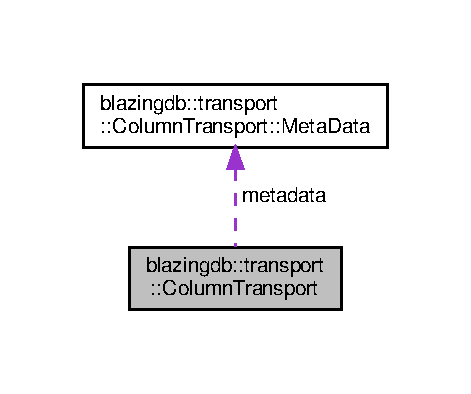
\includegraphics[width=226pt]{structblazingdb_1_1transport_1_1ColumnTransport__coll__graph}
\end{center}
\end{figure}
\subsection*{Classes}
\begin{DoxyCompactItemize}
\item 
struct \hyperlink{structblazingdb_1_1transport_1_1ColumnTransport_1_1MetaData}{Meta\+Data}
\end{DoxyCompactItemize}
\subsection*{Public Attributes}
\begin{DoxyCompactItemize}
\item 
\mbox{\Hypertarget{structblazingdb_1_1transport_1_1ColumnTransport_acf9500e94299bb1e6658731e6840fe16}\label{structblazingdb_1_1transport_1_1ColumnTransport_acf9500e94299bb1e6658731e6840fe16}} 
\hyperlink{structblazingdb_1_1transport_1_1ColumnTransport_1_1MetaData}{Meta\+Data} {\bfseries metadata} \{\}
\item 
\mbox{\Hypertarget{structblazingdb_1_1transport_1_1ColumnTransport_a425f4e29b911f369487f7229d6f51847}\label{structblazingdb_1_1transport_1_1ColumnTransport_a425f4e29b911f369487f7229d6f51847}} 
int {\bfseries data} \{\}
\item 
\mbox{\Hypertarget{structblazingdb_1_1transport_1_1ColumnTransport_ae8252232b90d35c7ef1281d37e297e82}\label{structblazingdb_1_1transport_1_1ColumnTransport_ae8252232b90d35c7ef1281d37e297e82}} 
int {\bfseries valid} \{\}
\item 
\mbox{\Hypertarget{structblazingdb_1_1transport_1_1ColumnTransport_aab04290a0ff26b843aa944e85d4072fe}\label{structblazingdb_1_1transport_1_1ColumnTransport_aab04290a0ff26b843aa944e85d4072fe}} 
int {\bfseries strings\+\_\+data} \{\}
\item 
\mbox{\Hypertarget{structblazingdb_1_1transport_1_1ColumnTransport_a82c325aab3b26ca3be341a1560137a47}\label{structblazingdb_1_1transport_1_1ColumnTransport_a82c325aab3b26ca3be341a1560137a47}} 
int {\bfseries strings\+\_\+offsets} \{\}
\item 
\mbox{\Hypertarget{structblazingdb_1_1transport_1_1ColumnTransport_a1756c2a5479abc9b6ba4d4f3163e1756}\label{structblazingdb_1_1transport_1_1ColumnTransport_a1756c2a5479abc9b6ba4d4f3163e1756}} 
int {\bfseries strings\+\_\+nullmask} \{\}
\item 
\mbox{\Hypertarget{structblazingdb_1_1transport_1_1ColumnTransport_a83f81a9f176c37204cc357937b10ce95}\label{structblazingdb_1_1transport_1_1ColumnTransport_a83f81a9f176c37204cc357937b10ce95}} 
int {\bfseries strings\+\_\+data\+\_\+size} \{0\}
\item 
\mbox{\Hypertarget{structblazingdb_1_1transport_1_1ColumnTransport_ae70474c73ba8318eb51cb2031702847d}\label{structblazingdb_1_1transport_1_1ColumnTransport_ae70474c73ba8318eb51cb2031702847d}} 
int {\bfseries strings\+\_\+offsets\+\_\+size} \{0\}
\item 
\mbox{\Hypertarget{structblazingdb_1_1transport_1_1ColumnTransport_a35528b121caf111beb1a984941d358af}\label{structblazingdb_1_1transport_1_1ColumnTransport_a35528b121caf111beb1a984941d358af}} 
std\+::size\+\_\+t {\bfseries size\+\_\+in\+\_\+bytes} \{0\}
\end{DoxyCompactItemize}


The documentation for this struct was generated from the following file\+:\begin{DoxyCompactItemize}
\item 
/home/tom/\+Documents/programming/romulo\+\_\+blazingsql/blazingsql/engine/src/transport/Column\+Transport.\+h\end{DoxyCompactItemize}

\hypertarget{classral_1_1communication_1_1CommunicationData}{}\section{ral\+:\+:communication\+:\+:Communication\+Data Class Reference}
\label{classral_1_1communication_1_1CommunicationData}\index{ral\+::communication\+::\+Communication\+Data@{ral\+::communication\+::\+Communication\+Data}}
\subsection*{Public Member Functions}
\begin{DoxyCompactItemize}
\item 
\mbox{\Hypertarget{classral_1_1communication_1_1CommunicationData_a54127850ce370846d7bec8838ac5977d}\label{classral_1_1communication_1_1CommunicationData_a54127850ce370846d7bec8838ac5977d}} 
void {\bfseries initialize} (const std\+::string \&worker\+\_\+id, const std\+::string \&cache\+\_\+directory)
\item 
\mbox{\Hypertarget{classral_1_1communication_1_1CommunicationData_a3760edb8d01a37ea1d2f4a22f79667c7}\label{classral_1_1communication_1_1CommunicationData_a3760edb8d01a37ea1d2f4a22f79667c7}} 
const \hyperlink{classblazingdb_1_1transport_1_1Node}{blazingdb\+::transport\+::\+Node} \& {\bfseries get\+Self\+Node} ()
\item 
\mbox{\Hypertarget{classral_1_1communication_1_1CommunicationData_a3ba22fbadc0e8ab7fa3ce3f4d2f14bde}\label{classral_1_1communication_1_1CommunicationData_a3ba22fbadc0e8ab7fa3ce3f4d2f14bde}} 
std\+::string {\bfseries get\+\_\+cache\+\_\+directory} ()
\item 
\mbox{\Hypertarget{classral_1_1communication_1_1CommunicationData_a06c1035a65f9f6732967f664c91046df}\label{classral_1_1communication_1_1CommunicationData_a06c1035a65f9f6732967f664c91046df}} 
{\bfseries Communication\+Data} (\hyperlink{classral_1_1communication_1_1CommunicationData}{Communication\+Data} \&\&)=delete
\item 
\mbox{\Hypertarget{classral_1_1communication_1_1CommunicationData_a921fb32cebb3abcd7b21e2100b5628c6}\label{classral_1_1communication_1_1CommunicationData_a921fb32cebb3abcd7b21e2100b5628c6}} 
{\bfseries Communication\+Data} (const \hyperlink{classral_1_1communication_1_1CommunicationData}{Communication\+Data} \&)=delete
\item 
\mbox{\Hypertarget{classral_1_1communication_1_1CommunicationData_a4e2f21a1e92329d1b7352e4778785841}\label{classral_1_1communication_1_1CommunicationData_a4e2f21a1e92329d1b7352e4778785841}} 
\hyperlink{classral_1_1communication_1_1CommunicationData}{Communication\+Data} \& {\bfseries operator=} (\hyperlink{classral_1_1communication_1_1CommunicationData}{Communication\+Data} \&\&)=delete
\item 
\mbox{\Hypertarget{classral_1_1communication_1_1CommunicationData_aa9fbd91e8d7d16b5075f037ddb01786f}\label{classral_1_1communication_1_1CommunicationData_aa9fbd91e8d7d16b5075f037ddb01786f}} 
\hyperlink{classral_1_1communication_1_1CommunicationData}{Communication\+Data} \& {\bfseries operator=} (const \hyperlink{classral_1_1communication_1_1CommunicationData}{Communication\+Data} \&)=delete
\end{DoxyCompactItemize}
\subsection*{Static Public Member Functions}
\begin{DoxyCompactItemize}
\item 
\mbox{\Hypertarget{classral_1_1communication_1_1CommunicationData_a5924a72dfc16fa5078ff30e9d7289e94}\label{classral_1_1communication_1_1CommunicationData_a5924a72dfc16fa5078ff30e9d7289e94}} 
static \hyperlink{classral_1_1communication_1_1CommunicationData}{Communication\+Data} \& {\bfseries get\+Instance} ()
\end{DoxyCompactItemize}


The documentation for this class was generated from the following files\+:\begin{DoxyCompactItemize}
\item 
/home/tom/\+Documents/programming/romulo\+\_\+blazingsql/blazingsql/engine/src/communication/Communication\+Data.\+h\item 
/home/tom/\+Documents/programming/romulo\+\_\+blazingsql/blazingsql/engine/src/communication/Communication\+Data.\+cpp\end{DoxyCompactItemize}

\hypertarget{classral_1_1batch_1_1ComputeAggregateKernel}{}\section{ral\+:\+:batch\+:\+:Compute\+Aggregate\+Kernel Class Reference}
\label{classral_1_1batch_1_1ComputeAggregateKernel}\index{ral\+::batch\+::\+Compute\+Aggregate\+Kernel@{ral\+::batch\+::\+Compute\+Aggregate\+Kernel}}


Inheritance diagram for ral\+:\+:batch\+:\+:Compute\+Aggregate\+Kernel\+:\nopagebreak
\begin{figure}[H]
\begin{center}
\leavevmode
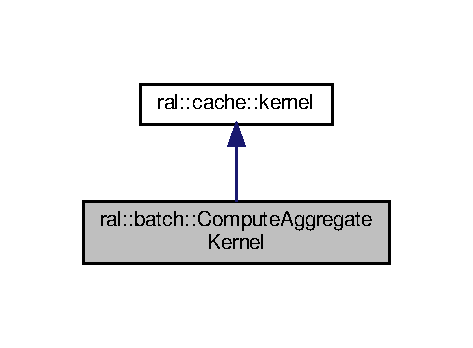
\includegraphics[width=227pt]{classral_1_1batch_1_1ComputeAggregateKernel__inherit__graph}
\end{center}
\end{figure}


Collaboration diagram for ral\+:\+:batch\+:\+:Compute\+Aggregate\+Kernel\+:\nopagebreak
\begin{figure}[H]
\begin{center}
\leavevmode
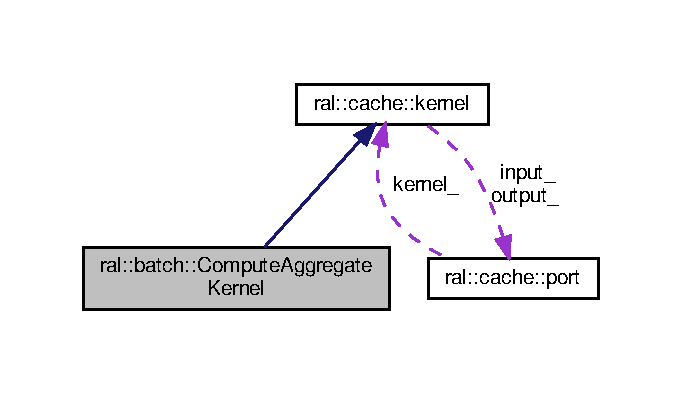
\includegraphics[width=328pt]{classral_1_1batch_1_1ComputeAggregateKernel__coll__graph}
\end{center}
\end{figure}
\subsection*{Public Member Functions}
\begin{DoxyCompactItemize}
\item 
\mbox{\Hypertarget{classral_1_1batch_1_1ComputeAggregateKernel_aa4be3582ee2fd8ac7af27261ec3ddc24}\label{classral_1_1batch_1_1ComputeAggregateKernel_aa4be3582ee2fd8ac7af27261ec3ddc24}} 
{\bfseries Compute\+Aggregate\+Kernel} (std\+::size\+\_\+t \hyperlink{classral_1_1cache_1_1kernel_a2fd708656cb056a41ec635b8bdc4acfe}{kernel\+\_\+id}, const std\+::string \&query\+String, std\+::shared\+\_\+ptr$<$ \hyperlink{classblazingdb_1_1manager_1_1Context}{Context} $>$ \hyperlink{classral_1_1cache_1_1kernel_af0347d14d678cfa7205c1387746a2e1b}{context}, std\+::shared\+\_\+ptr$<$ \hyperlink{classral_1_1cache_1_1graph}{ral\+::cache\+::graph} $>$ \hyperlink{classral_1_1cache_1_1kernel_a5fbb02292aff165a28ef25e75f0d89bd}{query\+\_\+graph})
\item 
\mbox{\Hypertarget{classral_1_1batch_1_1ComputeAggregateKernel_a70d6e3a23667950c3caa1ead353ef878}\label{classral_1_1batch_1_1ComputeAggregateKernel_a70d6e3a23667950c3caa1ead353ef878}} 
std\+::string {\bfseries kernel\+\_\+name} ()
\item 
\mbox{\Hypertarget{classral_1_1batch_1_1ComputeAggregateKernel_afa8069e21f3ad90f597e00c59ac064cd}\label{classral_1_1batch_1_1ComputeAggregateKernel_afa8069e21f3ad90f597e00c59ac064cd}} 
\hyperlink{structral_1_1execution_1_1task__result}{ral\+::execution\+::task\+\_\+result} {\bfseries do\+\_\+process} (std\+::vector$<$ std\+::unique\+\_\+ptr$<$ \hyperlink{classral_1_1frame_1_1BlazingTable}{ral\+::frame\+::\+Blazing\+Table} $>$ $>$ inputs, std\+::shared\+\_\+ptr$<$ \hyperlink{classral_1_1cache_1_1CacheMachine}{ral\+::cache\+::\+Cache\+Machine} $>$ output, cuda\+Stream\+\_\+t stream, const std\+::map$<$ std\+::string, std\+::string $>$ \&args) override
\item 
virtual kstatus \hyperlink{classral_1_1batch_1_1ComputeAggregateKernel_ad3f8e41cf0adf95dbe0249a6dd9c1240}{run} ()
\begin{DoxyCompactList}\small\item\em Executes the batch processing. Loads the data from their input port, and after processing it, the results are stored in their output port. \end{DoxyCompactList}\item 
\mbox{\Hypertarget{classral_1_1batch_1_1ComputeAggregateKernel_a08af1468040c590da06edee88cf92f2e}\label{classral_1_1batch_1_1ComputeAggregateKernel_a08af1468040c590da06edee88cf92f2e}} 
std\+::pair$<$ bool, uint64\+\_\+t $>$ \hyperlink{classral_1_1batch_1_1ComputeAggregateKernel_a08af1468040c590da06edee88cf92f2e}{get\+\_\+estimated\+\_\+output\+\_\+num\+\_\+rows} ()
\begin{DoxyCompactList}\small\item\em Returns the estimated num\+\_\+rows for the output, the default is that its the same as the input (i.\+e. project, sort, ...). \end{DoxyCompactList}\end{DoxyCompactItemize}
\subsection*{Additional Inherited Members}


\subsection{Member Function Documentation}
\mbox{\Hypertarget{classral_1_1batch_1_1ComputeAggregateKernel_ad3f8e41cf0adf95dbe0249a6dd9c1240}\label{classral_1_1batch_1_1ComputeAggregateKernel_ad3f8e41cf0adf95dbe0249a6dd9c1240}} 
\index{ral\+::batch\+::\+Compute\+Aggregate\+Kernel@{ral\+::batch\+::\+Compute\+Aggregate\+Kernel}!run@{run}}
\index{run@{run}!ral\+::batch\+::\+Compute\+Aggregate\+Kernel@{ral\+::batch\+::\+Compute\+Aggregate\+Kernel}}
\subsubsection{\texorpdfstring{run()}{run()}}
{\footnotesize\ttfamily kstatus ral\+::batch\+::\+Compute\+Aggregate\+Kernel\+::run (\begin{DoxyParamCaption}{ }\end{DoxyParamCaption})\hspace{0.3cm}{\ttfamily [virtual]}}



Executes the batch processing. Loads the data from their input port, and after processing it, the results are stored in their output port. 

\begin{DoxyReturn}{Returns}
kstatus \textquotesingle{}stop\textquotesingle{} to halt processing, or \textquotesingle{}proceed\textquotesingle{} to continue processing. 
\end{DoxyReturn}


Implements \hyperlink{classral_1_1cache_1_1kernel_a735b081cccae9574924e74ea6d293ef7}{ral\+::cache\+::kernel}.



The documentation for this class was generated from the following files\+:\begin{DoxyCompactItemize}
\item 
/home/tom/\+Documents/programming/romulo\+\_\+blazingsql/blazingsql/engine/src/execution\+\_\+graph/logic\+\_\+controllers/Batch\+Aggregation\+Processing.\+h\item 
/home/tom/\+Documents/programming/romulo\+\_\+blazingsql/blazingsql/engine/src/execution\+\_\+graph/logic\+\_\+controllers/Batch\+Aggregation\+Processing.\+cpp\end{DoxyCompactItemize}

\hypertarget{classral_1_1batch_1_1ComputeWindowKernel}{}\section{ral\+:\+:batch\+:\+:Compute\+Window\+Kernel Class Reference}
\label{classral_1_1batch_1_1ComputeWindowKernel}\index{ral\+::batch\+::\+Compute\+Window\+Kernel@{ral\+::batch\+::\+Compute\+Window\+Kernel}}


This kernel computes the main Window Function (R\+O\+W\+\_\+\+N\+U\+M\+B\+ER, L\+AG, L\+E\+AD, M\+IN, ...) to each batch already pattitioned and sorted New columns will be added to each batch.  




{\ttfamily \#include $<$Batch\+Window\+Function\+Processing.\+h$>$}



Inheritance diagram for ral\+:\+:batch\+:\+:Compute\+Window\+Kernel\+:\nopagebreak
\begin{figure}[H]
\begin{center}
\leavevmode
\includegraphics[width=218pt]{classral_1_1batch_1_1ComputeWindowKernel__inherit__graph}
\end{center}
\end{figure}


Collaboration diagram for ral\+:\+:batch\+:\+:Compute\+Window\+Kernel\+:\nopagebreak
\begin{figure}[H]
\begin{center}
\leavevmode
\includegraphics[width=318pt]{classral_1_1batch_1_1ComputeWindowKernel__coll__graph}
\end{center}
\end{figure}
\subsection*{Public Member Functions}
\begin{DoxyCompactItemize}
\item 
\mbox{\Hypertarget{classral_1_1batch_1_1ComputeWindowKernel_a1feff9b400748b38a36a91d7f256cd35}\label{classral_1_1batch_1_1ComputeWindowKernel_a1feff9b400748b38a36a91d7f256cd35}} 
{\bfseries Compute\+Window\+Kernel} (std\+::size\+\_\+t \hyperlink{classral_1_1cache_1_1kernel_a2fd708656cb056a41ec635b8bdc4acfe}{kernel\+\_\+id}, const std\+::string \&query\+String, std\+::shared\+\_\+ptr$<$ \hyperlink{classblazingdb_1_1manager_1_1Context}{Context} $>$ \hyperlink{classral_1_1cache_1_1kernel_af0347d14d678cfa7205c1387746a2e1b}{context}, std\+::shared\+\_\+ptr$<$ \hyperlink{classral_1_1cache_1_1graph}{ral\+::cache\+::graph} $>$ \hyperlink{classral_1_1cache_1_1kernel_a5fbb02292aff165a28ef25e75f0d89bd}{query\+\_\+graph})
\item 
\mbox{\Hypertarget{classral_1_1batch_1_1ComputeWindowKernel_a045546d30ebc87491d69757f8547c672}\label{classral_1_1batch_1_1ComputeWindowKernel_a045546d30ebc87491d69757f8547c672}} 
std\+::unique\+\_\+ptr$<$ Cudf\+Column $>$ {\bfseries compute\+\_\+column\+\_\+from\+\_\+window\+\_\+function} (cudf\+::table\+\_\+view input\+\_\+cudf\+\_\+view, cudf\+::column\+\_\+view input\+\_\+col\+\_\+view, std\+::size\+\_\+t pos, int \&agg\+\_\+param\+\_\+count)
\item 
\mbox{\Hypertarget{classral_1_1batch_1_1ComputeWindowKernel_a8caa7fbdb505758f1bcc465024a5cffa}\label{classral_1_1batch_1_1ComputeWindowKernel_a8caa7fbdb505758f1bcc465024a5cffa}} 
std\+::string {\bfseries kernel\+\_\+name} ()
\item 
\mbox{\Hypertarget{classral_1_1batch_1_1ComputeWindowKernel_a26873276168cdd25b055c313a50c0d2f}\label{classral_1_1batch_1_1ComputeWindowKernel_a26873276168cdd25b055c313a50c0d2f}} 
\hyperlink{structral_1_1execution_1_1task__result}{ral\+::execution\+::task\+\_\+result} {\bfseries do\+\_\+process} (std\+::vector$<$ std\+::unique\+\_\+ptr$<$ \hyperlink{classral_1_1frame_1_1BlazingTable}{ral\+::frame\+::\+Blazing\+Table} $>$ $>$ inputs, std\+::shared\+\_\+ptr$<$ \hyperlink{classral_1_1cache_1_1CacheMachine}{ral\+::cache\+::\+Cache\+Machine} $>$ output, cuda\+Stream\+\_\+t stream, const std\+::map$<$ std\+::string, std\+::string $>$ \&args) override
\item 
kstatus \hyperlink{classral_1_1batch_1_1ComputeWindowKernel_a22a36fbcb21dad09bad9300e21dc4825}{run} () override
\begin{DoxyCompactList}\small\item\em Executes the batch processing. Loads the data from their input port, and after processing it, the results are stored in their output port. \end{DoxyCompactList}\end{DoxyCompactItemize}
\subsection*{Additional Inherited Members}


\subsection{Detailed Description}
This kernel computes the main Window Function (R\+O\+W\+\_\+\+N\+U\+M\+B\+ER, L\+AG, L\+E\+AD, M\+IN, ...) to each batch already pattitioned and sorted New columns will be added to each batch. 

\subsection{Member Function Documentation}
\mbox{\Hypertarget{classral_1_1batch_1_1ComputeWindowKernel_a22a36fbcb21dad09bad9300e21dc4825}\label{classral_1_1batch_1_1ComputeWindowKernel_a22a36fbcb21dad09bad9300e21dc4825}} 
\index{ral\+::batch\+::\+Compute\+Window\+Kernel@{ral\+::batch\+::\+Compute\+Window\+Kernel}!run@{run}}
\index{run@{run}!ral\+::batch\+::\+Compute\+Window\+Kernel@{ral\+::batch\+::\+Compute\+Window\+Kernel}}
\subsubsection{\texorpdfstring{run()}{run()}}
{\footnotesize\ttfamily kstatus ral\+::batch\+::\+Compute\+Window\+Kernel\+::run (\begin{DoxyParamCaption}{ }\end{DoxyParamCaption})\hspace{0.3cm}{\ttfamily [override]}, {\ttfamily [virtual]}}



Executes the batch processing. Loads the data from their input port, and after processing it, the results are stored in their output port. 

\begin{DoxyReturn}{Returns}
kstatus \textquotesingle{}stop\textquotesingle{} to halt processing, or \textquotesingle{}proceed\textquotesingle{} to continue processing. 
\end{DoxyReturn}


Implements \hyperlink{classral_1_1cache_1_1kernel_a735b081cccae9574924e74ea6d293ef7}{ral\+::cache\+::kernel}.

Here is the call graph for this function\+:\nopagebreak
\begin{figure}[H]
\begin{center}
\leavevmode
\includegraphics[width=350pt]{classral_1_1batch_1_1ComputeWindowKernel_a22a36fbcb21dad09bad9300e21dc4825_cgraph}
\end{center}
\end{figure}


The documentation for this class was generated from the following files\+:\begin{DoxyCompactItemize}
\item 
/home/tom/\+Documents/programming/romulo\+\_\+blazingsql/blazingsql/engine/src/execution\+\_\+graph/logic\+\_\+controllers/Batch\+Window\+Function\+Processing.\+h\item 
/home/tom/\+Documents/programming/romulo\+\_\+blazingsql/blazingsql/engine/src/execution\+\_\+graph/logic\+\_\+controllers/Batch\+Window\+Function\+Processing.\+cpp\end{DoxyCompactItemize}

\hypertarget{classral_1_1cache_1_1ConcatCacheData}{}\section{ral\+:\+:cache\+:\+:Concat\+Cache\+Data Class Reference}
\label{classral_1_1cache_1_1ConcatCacheData}\index{ral\+::cache\+::\+Concat\+Cache\+Data@{ral\+::cache\+::\+Concat\+Cache\+Data}}


Inheritance diagram for ral\+:\+:cache\+:\+:Concat\+Cache\+Data\+:\nopagebreak
\begin{figure}[H]
\begin{center}
\leavevmode
\includegraphics[width=226pt]{classral_1_1cache_1_1ConcatCacheData__inherit__graph}
\end{center}
\end{figure}


Collaboration diagram for ral\+:\+:cache\+:\+:Concat\+Cache\+Data\+:\nopagebreak
\begin{figure}[H]
\begin{center}
\leavevmode
\includegraphics[width=230pt]{classral_1_1cache_1_1ConcatCacheData__coll__graph}
\end{center}
\end{figure}
\subsection*{Public Member Functions}
\begin{DoxyCompactItemize}
\item 
\hyperlink{classral_1_1cache_1_1ConcatCacheData_a9b88f49d90532642cb20be1de7f414c5}{Concat\+Cache\+Data} (std\+::vector$<$ std\+::unique\+\_\+ptr$<$ \hyperlink{classral_1_1cache_1_1CacheData}{Cache\+Data} $>$$>$ cache\+\_\+datas, const std\+::vector$<$ std\+::string $>$ \&\hyperlink{classral_1_1cache_1_1CacheData_a7a43a46a362c8fe93a7af81debbeca1b}{col\+\_\+names}, const std\+::vector$<$ cudf\+::data\+\_\+type $>$ \&\hyperlink{classral_1_1cache_1_1CacheData_aec9a1b3c0fb78cfdb3bd5494bcee2d8f}{schema})
\item 
std\+::unique\+\_\+ptr$<$ \hyperlink{classral_1_1frame_1_1BlazingTable}{ral\+::frame\+::\+Blazing\+Table} $>$ \hyperlink{classral_1_1cache_1_1ConcatCacheData_af726fc27fcf1621fff1f399f8b2d3cec}{decache} () override
\item 
size\+\_\+t \hyperlink{classral_1_1cache_1_1ConcatCacheData_a25914d06c36e4a1748dc9479adc5ccd8}{size\+In\+Bytes} () const override
\item 
void \hyperlink{classral_1_1cache_1_1ConcatCacheData_a02f400f33f88ba3e216f5899fa4f12b8}{set\+\_\+names} (const std\+::vector$<$ std\+::string $>$ \&\hyperlink{classral_1_1cache_1_1CacheData_aa2c8d58823d781cc1f8e6e589d897642}{names}) override
\item 
\mbox{\Hypertarget{classral_1_1cache_1_1ConcatCacheData_ab6b4c1d4bd8752827d522d8911547a1e}\label{classral_1_1cache_1_1ConcatCacheData_ab6b4c1d4bd8752827d522d8911547a1e}} 
std\+::vector$<$ std\+::unique\+\_\+ptr$<$ \hyperlink{classral_1_1cache_1_1CacheData}{Cache\+Data} $>$ $>$ {\bfseries release\+Cache\+Datas} ()
\end{DoxyCompactItemize}
\subsection*{Protected Attributes}
\begin{DoxyCompactItemize}
\item 
\mbox{\Hypertarget{classral_1_1cache_1_1ConcatCacheData_a420b449b6862f7db831e7e51acb6fee5}\label{classral_1_1cache_1_1ConcatCacheData_a420b449b6862f7db831e7e51acb6fee5}} 
std\+::vector$<$ std\+::unique\+\_\+ptr$<$ \hyperlink{classral_1_1cache_1_1CacheData}{Cache\+Data} $>$ $>$ {\bfseries \+\_\+cache\+\_\+datas}
\end{DoxyCompactItemize}
\subsection*{Additional Inherited Members}


\subsection{Constructor \& Destructor Documentation}
\mbox{\Hypertarget{classral_1_1cache_1_1ConcatCacheData_a9b88f49d90532642cb20be1de7f414c5}\label{classral_1_1cache_1_1ConcatCacheData_a9b88f49d90532642cb20be1de7f414c5}} 
\index{ral\+::cache\+::\+Concat\+Cache\+Data@{ral\+::cache\+::\+Concat\+Cache\+Data}!Concat\+Cache\+Data@{Concat\+Cache\+Data}}
\index{Concat\+Cache\+Data@{Concat\+Cache\+Data}!ral\+::cache\+::\+Concat\+Cache\+Data@{ral\+::cache\+::\+Concat\+Cache\+Data}}
\subsubsection{\texorpdfstring{Concat\+Cache\+Data()}{ConcatCacheData()}}
{\footnotesize\ttfamily ral\+::cache\+::\+Concat\+Cache\+Data\+::\+Concat\+Cache\+Data (\begin{DoxyParamCaption}\item[{std\+::vector$<$ std\+::unique\+\_\+ptr$<$ \hyperlink{classral_1_1cache_1_1CacheData}{Cache\+Data} $>$$>$}]{cache\+\_\+datas,  }\item[{const std\+::vector$<$ std\+::string $>$ \&}]{col\+\_\+names,  }\item[{const std\+::vector$<$ cudf\+::data\+\_\+type $>$ \&}]{schema }\end{DoxyParamCaption})}

Constructor 
\begin{DoxyParams}{Parameters}
{\em table} & The cache\+\_\+datas that will be concatenated when decached. \\
\hline
{\em col\+\_\+names} & The names of the columns in the dataframe. \\
\hline
{\em schema} & The types of the columns in the dataframe. \\
\hline
\end{DoxyParams}


\subsection{Member Function Documentation}
\mbox{\Hypertarget{classral_1_1cache_1_1ConcatCacheData_af726fc27fcf1621fff1f399f8b2d3cec}\label{classral_1_1cache_1_1ConcatCacheData_af726fc27fcf1621fff1f399f8b2d3cec}} 
\index{ral\+::cache\+::\+Concat\+Cache\+Data@{ral\+::cache\+::\+Concat\+Cache\+Data}!decache@{decache}}
\index{decache@{decache}!ral\+::cache\+::\+Concat\+Cache\+Data@{ral\+::cache\+::\+Concat\+Cache\+Data}}
\subsubsection{\texorpdfstring{decache()}{decache()}}
{\footnotesize\ttfamily std\+::unique\+\_\+ptr$<$ \hyperlink{classral_1_1frame_1_1BlazingTable}{ral\+::frame\+::\+Blazing\+Table} $>$ ral\+::cache\+::\+Concat\+Cache\+Data\+::decache (\begin{DoxyParamCaption}{ }\end{DoxyParamCaption})\hspace{0.3cm}{\ttfamily [override]}, {\ttfamily [virtual]}}

Decaches all caches datas and concatenates them into one Blazing\+Table \begin{DoxyReturn}{Returns}
The Blazing\+Table that results from concatenating all cache datas. 
\end{DoxyReturn}


Implements \hyperlink{classral_1_1cache_1_1CacheData_a2db8fdd2151babd7a07f4c6e246b710c}{ral\+::cache\+::\+Cache\+Data}.

\mbox{\Hypertarget{classral_1_1cache_1_1ConcatCacheData_a02f400f33f88ba3e216f5899fa4f12b8}\label{classral_1_1cache_1_1ConcatCacheData_a02f400f33f88ba3e216f5899fa4f12b8}} 
\index{ral\+::cache\+::\+Concat\+Cache\+Data@{ral\+::cache\+::\+Concat\+Cache\+Data}!set\+\_\+names@{set\+\_\+names}}
\index{set\+\_\+names@{set\+\_\+names}!ral\+::cache\+::\+Concat\+Cache\+Data@{ral\+::cache\+::\+Concat\+Cache\+Data}}
\subsubsection{\texorpdfstring{set\+\_\+names()}{set\_names()}}
{\footnotesize\ttfamily void ral\+::cache\+::\+Concat\+Cache\+Data\+::set\+\_\+names (\begin{DoxyParamCaption}\item[{const std\+::vector$<$ std\+::string $>$ \&}]{names }\end{DoxyParamCaption})\hspace{0.3cm}{\ttfamily [override]}, {\ttfamily [virtual]}}

Set the names of the columns. 
\begin{DoxyParams}{Parameters}
{\em names} & a vector of the column names. \\
\hline
\end{DoxyParams}


Implements \hyperlink{classral_1_1cache_1_1CacheData_a3bb1623a4266ba7c961d325023ff13c6}{ral\+::cache\+::\+Cache\+Data}.

\mbox{\Hypertarget{classral_1_1cache_1_1ConcatCacheData_a25914d06c36e4a1748dc9479adc5ccd8}\label{classral_1_1cache_1_1ConcatCacheData_a25914d06c36e4a1748dc9479adc5ccd8}} 
\index{ral\+::cache\+::\+Concat\+Cache\+Data@{ral\+::cache\+::\+Concat\+Cache\+Data}!size\+In\+Bytes@{size\+In\+Bytes}}
\index{size\+In\+Bytes@{size\+In\+Bytes}!ral\+::cache\+::\+Concat\+Cache\+Data@{ral\+::cache\+::\+Concat\+Cache\+Data}}
\subsubsection{\texorpdfstring{size\+In\+Bytes()}{sizeInBytes()}}
{\footnotesize\ttfamily size\+\_\+t ral\+::cache\+::\+Concat\+Cache\+Data\+::size\+In\+Bytes (\begin{DoxyParamCaption}{ }\end{DoxyParamCaption}) const\hspace{0.3cm}{\ttfamily [override]}, {\ttfamily [virtual]}}

Get the amount of G\+PU memory consumed by this \hyperlink{classral_1_1cache_1_1CacheData}{Cache\+Data} Having this function allows us to have one api for seeing the consumption of all the \hyperlink{classral_1_1cache_1_1CacheData}{Cache\+Data} objects that are currently in Caches. \begin{DoxyReturn}{Returns}
The number of bytes the Blazing\+Table consumes. 
\end{DoxyReturn}


Implements \hyperlink{classral_1_1cache_1_1CacheData_aaad8a726296574845f01f9380dcee40d}{ral\+::cache\+::\+Cache\+Data}.



The documentation for this class was generated from the following files\+:\begin{DoxyCompactItemize}
\item 
/home/tom/\+Documents/programming/romulo\+\_\+blazingsql/blazingsql/engine/src/execution\+\_\+graph/logic\+\_\+controllers/Cache\+Data.\+h\item 
/home/tom/\+Documents/programming/romulo\+\_\+blazingsql/blazingsql/engine/src/execution\+\_\+graph/logic\+\_\+controllers/Cache\+Data.\+cpp\end{DoxyCompactItemize}

\hypertarget{classral_1_1cache_1_1ConcatenatingCacheMachine}{}\section{ral\+:\+:cache\+:\+:Concatenating\+Cache\+Machine Class Reference}
\label{classral_1_1cache_1_1ConcatenatingCacheMachine}\index{ral\+::cache\+::\+Concatenating\+Cache\+Machine@{ral\+::cache\+::\+Concatenating\+Cache\+Machine}}


A class that represents a Cache Machine on a multi-\/tier cache system. Moreover, it only returns a single Blazing\+Table by concatenating all batches. This Cache Machine is used in the last Kernel (Output\+Kernel) in the Execution\+Graph.  




{\ttfamily \#include $<$Cache\+Machine.\+h$>$}



Inheritance diagram for ral\+:\+:cache\+:\+:Concatenating\+Cache\+Machine\+:\nopagebreak
\begin{figure}[H]
\begin{center}
\leavevmode
\includegraphics[width=211pt]{classral_1_1cache_1_1ConcatenatingCacheMachine__inherit__graph}
\end{center}
\end{figure}


Collaboration diagram for ral\+:\+:cache\+:\+:Concatenating\+Cache\+Machine\+:\nopagebreak
\begin{figure}[H]
\begin{center}
\leavevmode
\includegraphics[width=211pt]{classral_1_1cache_1_1ConcatenatingCacheMachine__coll__graph}
\end{center}
\end{figure}
\subsection*{Public Member Functions}
\begin{DoxyCompactItemize}
\item 
\mbox{\Hypertarget{classral_1_1cache_1_1ConcatenatingCacheMachine_ac63a832595832d436951d12acfb11971}\label{classral_1_1cache_1_1ConcatenatingCacheMachine_ac63a832595832d436951d12acfb11971}} 
{\bfseries Concatenating\+Cache\+Machine} (std\+::shared\+\_\+ptr$<$ \hyperlink{classblazingdb_1_1manager_1_1Context}{Context} $>$ context, std\+::string cache\+\_\+machine\+\_\+name)
\item 
\mbox{\Hypertarget{classral_1_1cache_1_1ConcatenatingCacheMachine_a965ed85fea8f3dfec4792fbac8001391}\label{classral_1_1cache_1_1ConcatenatingCacheMachine_a965ed85fea8f3dfec4792fbac8001391}} 
{\bfseries Concatenating\+Cache\+Machine} (std\+::shared\+\_\+ptr$<$ \hyperlink{classblazingdb_1_1manager_1_1Context}{Context} $>$ context, std\+::size\+\_\+t concat\+\_\+cache\+\_\+num\+\_\+bytes, bool concat\+\_\+all, std\+::string cache\+\_\+machine\+\_\+name)
\item 
\mbox{\Hypertarget{classral_1_1cache_1_1ConcatenatingCacheMachine_a0dc01ef4e13b5f832d52f2d07d1f1f69}\label{classral_1_1cache_1_1ConcatenatingCacheMachine_a0dc01ef4e13b5f832d52f2d07d1f1f69}} 
std\+::unique\+\_\+ptr$<$ \hyperlink{classral_1_1frame_1_1BlazingTable}{ral\+::frame\+::\+Blazing\+Table} $>$ {\bfseries pull\+From\+Cache} () override
\item 
\mbox{\Hypertarget{classral_1_1cache_1_1ConcatenatingCacheMachine_a9c8db51d9971f78ff74134db114bb69a}\label{classral_1_1cache_1_1ConcatenatingCacheMachine_a9c8db51d9971f78ff74134db114bb69a}} 
std\+::unique\+\_\+ptr$<$ \hyperlink{classral_1_1frame_1_1BlazingTable}{ral\+::frame\+::\+Blazing\+Table} $>$ {\bfseries pull\+Unordered\+From\+Cache} () override
\item 
\mbox{\Hypertarget{classral_1_1cache_1_1ConcatenatingCacheMachine_af02b87583c465b8d90b451288e16cdc5}\label{classral_1_1cache_1_1ConcatenatingCacheMachine_af02b87583c465b8d90b451288e16cdc5}} 
std\+::unique\+\_\+ptr$<$ \hyperlink{classral_1_1cache_1_1CacheData}{ral\+::cache\+::\+Cache\+Data} $>$ {\bfseries pull\+Cache\+Data} () override
\item 
\mbox{\Hypertarget{classral_1_1cache_1_1ConcatenatingCacheMachine_a04db0538230cd10cf7ae4ebc1cd62167}\label{classral_1_1cache_1_1ConcatenatingCacheMachine_a04db0538230cd10cf7ae4ebc1cd62167}} 
size\+\_\+t {\bfseries downgrade\+Cache\+Data} () override
\end{DoxyCompactItemize}
\subsection*{Additional Inherited Members}


\subsection{Detailed Description}
A class that represents a Cache Machine on a multi-\/tier cache system. Moreover, it only returns a single Blazing\+Table by concatenating all batches. This Cache Machine is used in the last Kernel (Output\+Kernel) in the Execution\+Graph. 

This Concatenating\+Cache\+Machine\+::pull\+From\+Cache method does not guarantee the relative order of the messages to be preserved 

The documentation for this class was generated from the following files\+:\begin{DoxyCompactItemize}
\item 
/home/tom/\+Documents/programming/romulo\+\_\+blazingsql/blazingsql/engine/src/execution\+\_\+graph/logic\+\_\+controllers/Cache\+Machine.\+h\item 
/home/tom/\+Documents/programming/romulo\+\_\+blazingsql/blazingsql/engine/src/execution\+\_\+graph/logic\+\_\+controllers/Cache\+Machine.\+cpp\end{DoxyCompactItemize}

\hypertarget{classblazingdb_1_1manager_1_1Context}{}\section{blazingdb\+:\+:manager\+:\+:Context Class Reference}
\label{classblazingdb_1_1manager_1_1Context}\index{blazingdb\+::manager\+::\+Context@{blazingdb\+::manager\+::\+Context}}


This is the main component of the transport library.  




{\ttfamily \#include $<$Context.\+h$>$}

\subsection*{Public Member Functions}
\begin{DoxyCompactItemize}
\item 
\mbox{\Hypertarget{classblazingdb_1_1manager_1_1Context_a06497a0c2a975edaefeb70077bed281c}\label{classblazingdb_1_1manager_1_1Context_a06497a0c2a975edaefeb70077bed281c}} 
{\bfseries Context} (const uint32\+\_\+t token, const std\+::vector$<$ \hyperlink{classblazingdb_1_1transport_1_1Node}{Node} $>$ \&task\+Nodes, const \hyperlink{classblazingdb_1_1transport_1_1Node}{Node} \&master\+Node, const std\+::string \&logical\+Plan, const std\+::map$<$ std\+::string, std\+::string $>$ \&config\+\_\+options)
\item 
\mbox{\Hypertarget{classblazingdb_1_1manager_1_1Context_a2e7dc296d717126eb032ab3f55742531}\label{classblazingdb_1_1manager_1_1Context_a2e7dc296d717126eb032ab3f55742531}} 
std\+::shared\+\_\+ptr$<$ \hyperlink{classblazingdb_1_1manager_1_1Context}{Context} $>$ {\bfseries clone} ()
\item 
\mbox{\Hypertarget{classblazingdb_1_1manager_1_1Context_a19e76e2eec88f05dbbb4dc54600c2ea4}\label{classblazingdb_1_1manager_1_1Context_a19e76e2eec88f05dbbb4dc54600c2ea4}} 
int {\bfseries get\+Total\+Nodes} () const
\item 
\mbox{\Hypertarget{classblazingdb_1_1manager_1_1Context_a1107a1de655b5904b4bff8f4db648fa6}\label{classblazingdb_1_1manager_1_1Context_a1107a1de655b5904b4bff8f4db648fa6}} 
std\+::vector$<$ \hyperlink{classblazingdb_1_1transport_1_1Node}{Node} $>$ {\bfseries get\+All\+Nodes} () const
\item 
\mbox{\Hypertarget{classblazingdb_1_1manager_1_1Context_a8145e32076548759fa9163dd1fe13ccf}\label{classblazingdb_1_1manager_1_1Context_a8145e32076548759fa9163dd1fe13ccf}} 
std\+::vector$<$ \hyperlink{classblazingdb_1_1transport_1_1Node}{Node} $>$ {\bfseries get\+All\+Other\+Nodes} (int self\+Node\+Index) const
\item 
\mbox{\Hypertarget{classblazingdb_1_1manager_1_1Context_a4aa25b97a3c3e96e10947f519d171b35}\label{classblazingdb_1_1manager_1_1Context_a4aa25b97a3c3e96e10947f519d171b35}} 
std\+::vector$<$ \hyperlink{classblazingdb_1_1transport_1_1Node}{Node} $>$ \hyperlink{classblazingdb_1_1manager_1_1Context_a4aa25b97a3c3e96e10947f519d171b35}{get\+Worker\+Nodes} () const
\begin{DoxyCompactList}\small\item\em R\+AL instances that will run the query. \end{DoxyCompactList}\item 
\mbox{\Hypertarget{classblazingdb_1_1manager_1_1Context_af31d1d36d220e0d84f30280f18c0dab1}\label{classblazingdb_1_1manager_1_1Context_af31d1d36d220e0d84f30280f18c0dab1}} 
\hyperlink{classblazingdb_1_1transport_1_1Node}{Node} {\bfseries get\+Node} (int node\+\_\+index) const
\item 
\mbox{\Hypertarget{classblazingdb_1_1manager_1_1Context_a825bc87492256cd9c0edad4ee8b1928a}\label{classblazingdb_1_1manager_1_1Context_a825bc87492256cd9c0edad4ee8b1928a}} 
\hyperlink{classblazingdb_1_1transport_1_1Node}{Node} {\bfseries get\+Node} (const std\+::string \&id) const
\item 
const \hyperlink{classblazingdb_1_1transport_1_1Node}{Node} \& \hyperlink{classblazingdb_1_1manager_1_1Context_ad1faee75fb1b10af373d6481ae621dfd}{get\+Master\+Node} () const
\item 
std\+::string \hyperlink{classblazingdb_1_1manager_1_1Context_ae0093ffa619c372c6130af7e3c77c372}{get\+Logical\+Plan} () const
\item 
\mbox{\Hypertarget{classblazingdb_1_1manager_1_1Context_a8e4398b9941b94007cae1b5c53a35008}\label{classblazingdb_1_1manager_1_1Context_a8e4398b9941b94007cae1b5c53a35008}} 
uint32\+\_\+t {\bfseries get\+Context\+Token} () const
\item 
\mbox{\Hypertarget{classblazingdb_1_1manager_1_1Context_aea67cc180a62a0ae6772ecdbe67e941a}\label{classblazingdb_1_1manager_1_1Context_aea67cc180a62a0ae6772ecdbe67e941a}} 
std\+::string {\bfseries get\+Context\+Communication\+Token} () const
\item 
\mbox{\Hypertarget{classblazingdb_1_1manager_1_1Context_a96fe3bf29e74bb9ed00f0062eda99676}\label{classblazingdb_1_1manager_1_1Context_a96fe3bf29e74bb9ed00f0062eda99676}} 
void {\bfseries increment\+Query\+Step} ()
\item 
\mbox{\Hypertarget{classblazingdb_1_1manager_1_1Context_aad6b4624ca3925ed5395159b330f4f9f}\label{classblazingdb_1_1manager_1_1Context_aad6b4624ca3925ed5395159b330f4f9f}} 
void {\bfseries increment\+Query\+Substep} ()
\item 
\mbox{\Hypertarget{classblazingdb_1_1manager_1_1Context_a99a062320c7d2d3acdaa876635a96f1b}\label{classblazingdb_1_1manager_1_1Context_a99a062320c7d2d3acdaa876635a96f1b}} 
uint32\+\_\+t {\bfseries get\+Query\+Step} () const
\item 
\mbox{\Hypertarget{classblazingdb_1_1manager_1_1Context_ab8982de5aaebf8f29c0f1d86cf4c84d6}\label{classblazingdb_1_1manager_1_1Context_ab8982de5aaebf8f29c0f1d86cf4c84d6}} 
uint32\+\_\+t {\bfseries get\+Query\+Substep} () const
\item 
\mbox{\Hypertarget{classblazingdb_1_1manager_1_1Context_a087b4b0ced49313fbc9c3b3994aa870e}\label{classblazingdb_1_1manager_1_1Context_a087b4b0ced49313fbc9c3b3994aa870e}} 
int {\bfseries get\+Node\+Index} (const \hyperlink{classblazingdb_1_1transport_1_1Node}{Node} \&node) const
\item 
\mbox{\Hypertarget{classblazingdb_1_1manager_1_1Context_ae7a8106947af5b4500760fb761a86788}\label{classblazingdb_1_1manager_1_1Context_ae7a8106947af5b4500760fb761a86788}} 
bool {\bfseries is\+Master\+Node} (const \hyperlink{classblazingdb_1_1transport_1_1Node}{Node} \&node) const
\item 
\mbox{\Hypertarget{classblazingdb_1_1manager_1_1Context_a428622bfe697d0d6f4ace3c0c6cef9fd}\label{classblazingdb_1_1manager_1_1Context_a428622bfe697d0d6f4ace3c0c6cef9fd}} 
void {\bfseries set\+Kernel\+Id} (uint32\+\_\+t kernel\+\_\+id)
\item 
\mbox{\Hypertarget{classblazingdb_1_1manager_1_1Context_a7fa93aeb80ef105da3c812b9da732e5d}\label{classblazingdb_1_1manager_1_1Context_a7fa93aeb80ef105da3c812b9da732e5d}} 
uint32\+\_\+t {\bfseries get\+Kernel\+Id} () const
\item 
\mbox{\Hypertarget{classblazingdb_1_1manager_1_1Context_a7ea6b41e017024e6ab010998ccc40b06}\label{classblazingdb_1_1manager_1_1Context_a7ea6b41e017024e6ab010998ccc40b06}} 
std\+::map$<$ std\+::string, std\+::string $>$ {\bfseries get\+Config\+Options} () const
\end{DoxyCompactItemize}


\subsection{Detailed Description}
This is the main component of the transport library. 

Manage and group the Node \textquotesingle{}s (task nodes) to be used by an specific query. 

\subsection{Member Function Documentation}
\mbox{\Hypertarget{classblazingdb_1_1manager_1_1Context_ae0093ffa619c372c6130af7e3c77c372}\label{classblazingdb_1_1manager_1_1Context_ae0093ffa619c372c6130af7e3c77c372}} 
\index{blazingdb\+::manager\+::\+Context@{blazingdb\+::manager\+::\+Context}!get\+Logical\+Plan@{get\+Logical\+Plan}}
\index{get\+Logical\+Plan@{get\+Logical\+Plan}!blazingdb\+::manager\+::\+Context@{blazingdb\+::manager\+::\+Context}}
\subsubsection{\texorpdfstring{get\+Logical\+Plan()}{getLogicalPlan()}}
{\footnotesize\ttfamily std\+::string blazingdb\+::manager\+::\+Context\+::get\+Logical\+Plan (\begin{DoxyParamCaption}{ }\end{DoxyParamCaption}) const}

\begin{DoxyRefDesc}{Deprecated}
\item[\hyperlink{deprecated__deprecated000001}{Deprecated}]\+: not used anymore \end{DoxyRefDesc}
\mbox{\Hypertarget{classblazingdb_1_1manager_1_1Context_ad1faee75fb1b10af373d6481ae621dfd}\label{classblazingdb_1_1manager_1_1Context_ad1faee75fb1b10af373d6481ae621dfd}} 
\index{blazingdb\+::manager\+::\+Context@{blazingdb\+::manager\+::\+Context}!get\+Master\+Node@{get\+Master\+Node}}
\index{get\+Master\+Node@{get\+Master\+Node}!blazingdb\+::manager\+::\+Context@{blazingdb\+::manager\+::\+Context}}
\subsubsection{\texorpdfstring{get\+Master\+Node()}{getMasterNode()}}
{\footnotesize\ttfamily const \hyperlink{classblazingdb_1_1transport_1_1Node}{Node} \& blazingdb\+::manager\+::\+Context\+::get\+Master\+Node (\begin{DoxyParamCaption}{ }\end{DoxyParamCaption}) const}

A single unique R\+AL instance that helps to the messages transmition and processesing between worker R\+AL\textquotesingle{}s e.\+g.\+: see Sample\+To\+Node\+Master\+Message 

The documentation for this class was generated from the following files\+:\begin{DoxyCompactItemize}
\item 
/home/tom/\+Documents/programming/romulo\+\_\+blazingsql/blazingsql/engine/src/execution\+\_\+graph/Context.\+h\item 
/home/tom/\+Documents/programming/romulo\+\_\+blazingsql/blazingsql/engine/src/execution\+\_\+graph/Context.\+cpp\end{DoxyCompactItemize}

\hypertarget{classral_1_1cache_1_1CPUCacheData}{}\section{ral\+:\+:cache\+:\+:C\+P\+U\+Cache\+Data Class Reference}
\label{classral_1_1cache_1_1CPUCacheData}\index{ral\+::cache\+::\+C\+P\+U\+Cache\+Data@{ral\+::cache\+::\+C\+P\+U\+Cache\+Data}}


{\ttfamily \#include $<$Cache\+Data.\+h$>$}



Inheritance diagram for ral\+:\+:cache\+:\+:C\+P\+U\+Cache\+Data\+:\nopagebreak
\begin{figure}[H]
\begin{center}
\leavevmode
\includegraphics[width=217pt]{classral_1_1cache_1_1CPUCacheData__inherit__graph}
\end{center}
\end{figure}


Collaboration diagram for ral\+:\+:cache\+:\+:C\+P\+U\+Cache\+Data\+:\nopagebreak
\begin{figure}[H]
\begin{center}
\leavevmode
\includegraphics[width=230pt]{classral_1_1cache_1_1CPUCacheData__coll__graph}
\end{center}
\end{figure}
\subsection*{Public Member Functions}
\begin{DoxyCompactItemize}
\item 
\hyperlink{classral_1_1cache_1_1CPUCacheData_a0b647a41636c90cd2992a2cc11994af1}{C\+P\+U\+Cache\+Data} (std\+::unique\+\_\+ptr$<$ \hyperlink{classral_1_1frame_1_1BlazingTable}{ral\+::frame\+::\+Blazing\+Table} $>$ gpu\+\_\+table, bool use\+\_\+pinned=false)
\item 
\mbox{\Hypertarget{classral_1_1cache_1_1CPUCacheData_a3d3d74db3db35f1f60008e7e28c5a5c6}\label{classral_1_1cache_1_1CPUCacheData_a3d3d74db3db35f1f60008e7e28c5a5c6}} 
{\bfseries C\+P\+U\+Cache\+Data} (std\+::unique\+\_\+ptr$<$ \hyperlink{classral_1_1frame_1_1BlazingTable}{ral\+::frame\+::\+Blazing\+Table} $>$ gpu\+\_\+table, const \hyperlink{classral_1_1cache_1_1MetadataDictionary}{Metadata\+Dictionary} \&\hyperlink{classral_1_1cache_1_1CacheData_aaeb232ef3aa8c2a3d86e1169ed2e8152}{metadata}, bool use\+\_\+pinned=false)
\item 
\mbox{\Hypertarget{classral_1_1cache_1_1CPUCacheData_a55d89069b138a46d2ea591546a26c6b5}\label{classral_1_1cache_1_1CPUCacheData_a55d89069b138a46d2ea591546a26c6b5}} 
{\bfseries C\+P\+U\+Cache\+Data} (const std\+::vector$<$ \hyperlink{structblazingdb_1_1transport_1_1ColumnTransport}{blazingdb\+::transport\+::\+Column\+Transport} $>$ \&column\+\_\+transports, std\+::vector$<$ \hyperlink{structral_1_1memory_1_1blazing__chunked__column__info}{ral\+::memory\+::blazing\+\_\+chunked\+\_\+column\+\_\+info} $>$ \&\&chunked\+\_\+column\+\_\+infos, std\+::vector$<$ std\+::unique\+\_\+ptr$<$ \hyperlink{structral_1_1memory_1_1blazing__allocation__chunk}{ral\+::memory\+::blazing\+\_\+allocation\+\_\+chunk} $>$$>$ \&\&allocations, const \hyperlink{classral_1_1cache_1_1MetadataDictionary}{Metadata\+Dictionary} \&\hyperlink{classral_1_1cache_1_1CacheData_aaeb232ef3aa8c2a3d86e1169ed2e8152}{metadata})
\item 
\hyperlink{classral_1_1cache_1_1CPUCacheData_ae74c9b51edabc2aa06f8923c6f3afc5f}{C\+P\+U\+Cache\+Data} (std\+::unique\+\_\+ptr$<$ \hyperlink{classral_1_1frame_1_1BlazingHostTable}{ral\+::frame\+::\+Blazing\+Host\+Table} $>$ \hyperlink{classral_1_1cache_1_1CPUCacheData_ae46ccefa906792a3b31bbd94e7fdcef1}{host\+\_\+table})
\item 
std\+::unique\+\_\+ptr$<$ \hyperlink{classral_1_1frame_1_1BlazingTable}{ral\+::frame\+::\+Blazing\+Table} $>$ \hyperlink{classral_1_1cache_1_1CPUCacheData_a03a18d3dfd4fe60dffdd0a9daabfbde2}{decache} () override
\item 
std\+::unique\+\_\+ptr$<$ \hyperlink{classral_1_1frame_1_1BlazingHostTable}{ral\+::frame\+::\+Blazing\+Host\+Table} $>$ \hyperlink{classral_1_1cache_1_1CPUCacheData_a817e6a8d23b4839f4e77c102a4ac0aad}{release\+Host\+Table} ()
\item 
size\+\_\+t \hyperlink{classral_1_1cache_1_1CPUCacheData_a83236d09b1d2341059d1a6738839d35c}{size\+In\+Bytes} () const override
\item 
void \hyperlink{classral_1_1cache_1_1CPUCacheData_a3d0444ff9ba0814775499060071a2d1a}{set\+\_\+names} (const std\+::vector$<$ std\+::string $>$ \&\hyperlink{classral_1_1cache_1_1CacheData_aa2c8d58823d781cc1f8e6e589d897642}{names}) override
\item 
virtual \hyperlink{classral_1_1cache_1_1CPUCacheData_acae066424ccf0651bcb17f54aa770bbb}{$\sim$\+C\+P\+U\+Cache\+Data} ()
\end{DoxyCompactItemize}
\subsection*{Protected Attributes}
\begin{DoxyCompactItemize}
\item 
std\+::unique\+\_\+ptr$<$ \hyperlink{classral_1_1frame_1_1BlazingHostTable}{ral\+::frame\+::\+Blazing\+Host\+Table} $>$ \hyperlink{classral_1_1cache_1_1CPUCacheData_ae46ccefa906792a3b31bbd94e7fdcef1}{host\+\_\+table}
\end{DoxyCompactItemize}
\subsection*{Additional Inherited Members}


\subsection{Detailed Description}
A \hyperlink{classral_1_1cache_1_1CacheData}{Cache\+Data} that keeps its dataframe in C\+PU memory. This is a \hyperlink{classral_1_1cache_1_1CacheData}{Cache\+Data} representation that wraps a \hyperlink{classral_1_1frame_1_1BlazingHostTable}{ral\+::frame\+::\+Blazing\+Host\+Table}. It is the more performant than most file based caching strategies but less efficient than a \hyperlink{classral_1_1cache_1_1GPUCacheData}{G\+P\+U\+Cache\+Data}. 

\subsection{Constructor \& Destructor Documentation}
\mbox{\Hypertarget{classral_1_1cache_1_1CPUCacheData_a0b647a41636c90cd2992a2cc11994af1}\label{classral_1_1cache_1_1CPUCacheData_a0b647a41636c90cd2992a2cc11994af1}} 
\index{ral\+::cache\+::\+C\+P\+U\+Cache\+Data@{ral\+::cache\+::\+C\+P\+U\+Cache\+Data}!C\+P\+U\+Cache\+Data@{C\+P\+U\+Cache\+Data}}
\index{C\+P\+U\+Cache\+Data@{C\+P\+U\+Cache\+Data}!ral\+::cache\+::\+C\+P\+U\+Cache\+Data@{ral\+::cache\+::\+C\+P\+U\+Cache\+Data}}
\subsubsection{\texorpdfstring{C\+P\+U\+Cache\+Data()}{CPUCacheData()}\hspace{0.1cm}{\footnotesize\ttfamily [1/2]}}
{\footnotesize\ttfamily ral\+::cache\+::\+C\+P\+U\+Cache\+Data\+::\+C\+P\+U\+Cache\+Data (\begin{DoxyParamCaption}\item[{std\+::unique\+\_\+ptr$<$ \hyperlink{classral_1_1frame_1_1BlazingTable}{ral\+::frame\+::\+Blazing\+Table} $>$}]{gpu\+\_\+table,  }\item[{bool}]{use\+\_\+pinned = {\ttfamily false} }\end{DoxyParamCaption})}

Constructor Takes a G\+PU based \hyperlink{classral_1_1frame_1_1BlazingTable}{ral\+::frame\+::\+Blazing\+Table} and converts it C\+PU version that is stored in a \hyperlink{classral_1_1frame_1_1BlazingHostTable}{ral\+::frame\+::\+Blazing\+Host\+Table}. 
\begin{DoxyParams}{Parameters}
{\em table} & The Blazing\+Table that is converted to a Blazing\+Host\+Table and stored. \\
\hline
\end{DoxyParams}
\mbox{\Hypertarget{classral_1_1cache_1_1CPUCacheData_ae74c9b51edabc2aa06f8923c6f3afc5f}\label{classral_1_1cache_1_1CPUCacheData_ae74c9b51edabc2aa06f8923c6f3afc5f}} 
\index{ral\+::cache\+::\+C\+P\+U\+Cache\+Data@{ral\+::cache\+::\+C\+P\+U\+Cache\+Data}!C\+P\+U\+Cache\+Data@{C\+P\+U\+Cache\+Data}}
\index{C\+P\+U\+Cache\+Data@{C\+P\+U\+Cache\+Data}!ral\+::cache\+::\+C\+P\+U\+Cache\+Data@{ral\+::cache\+::\+C\+P\+U\+Cache\+Data}}
\subsubsection{\texorpdfstring{C\+P\+U\+Cache\+Data()}{CPUCacheData()}\hspace{0.1cm}{\footnotesize\ttfamily [2/2]}}
{\footnotesize\ttfamily ral\+::cache\+::\+C\+P\+U\+Cache\+Data\+::\+C\+P\+U\+Cache\+Data (\begin{DoxyParamCaption}\item[{std\+::unique\+\_\+ptr$<$ \hyperlink{classral_1_1frame_1_1BlazingHostTable}{ral\+::frame\+::\+Blazing\+Host\+Table} $>$}]{host\+\_\+table }\end{DoxyParamCaption})}

Constructor Takes a G\+PU based \hyperlink{classral_1_1frame_1_1BlazingHostTable}{ral\+::frame\+::\+Blazing\+Host\+Table} and stores it in this \hyperlink{classral_1_1cache_1_1CacheData}{Cache\+Data} instance. 
\begin{DoxyParams}{Parameters}
{\em table} & The Blazing\+Host\+Table that is moved into the \hyperlink{classral_1_1cache_1_1CacheData}{Cache\+Data}. \\
\hline
\end{DoxyParams}
\mbox{\Hypertarget{classral_1_1cache_1_1CPUCacheData_acae066424ccf0651bcb17f54aa770bbb}\label{classral_1_1cache_1_1CPUCacheData_acae066424ccf0651bcb17f54aa770bbb}} 
\index{ral\+::cache\+::\+C\+P\+U\+Cache\+Data@{ral\+::cache\+::\+C\+P\+U\+Cache\+Data}!````~C\+P\+U\+Cache\+Data@{$\sim$\+C\+P\+U\+Cache\+Data}}
\index{````~C\+P\+U\+Cache\+Data@{$\sim$\+C\+P\+U\+Cache\+Data}!ral\+::cache\+::\+C\+P\+U\+Cache\+Data@{ral\+::cache\+::\+C\+P\+U\+Cache\+Data}}
\subsubsection{\texorpdfstring{$\sim$\+C\+P\+U\+Cache\+Data()}{~CPUCacheData()}}
{\footnotesize\ttfamily virtual ral\+::cache\+::\+C\+P\+U\+Cache\+Data\+::$\sim$\+C\+P\+U\+Cache\+Data (\begin{DoxyParamCaption}{ }\end{DoxyParamCaption})\hspace{0.3cm}{\ttfamily [inline]}, {\ttfamily [virtual]}}

Destructor 

\subsection{Member Function Documentation}
\mbox{\Hypertarget{classral_1_1cache_1_1CPUCacheData_a03a18d3dfd4fe60dffdd0a9daabfbde2}\label{classral_1_1cache_1_1CPUCacheData_a03a18d3dfd4fe60dffdd0a9daabfbde2}} 
\index{ral\+::cache\+::\+C\+P\+U\+Cache\+Data@{ral\+::cache\+::\+C\+P\+U\+Cache\+Data}!decache@{decache}}
\index{decache@{decache}!ral\+::cache\+::\+C\+P\+U\+Cache\+Data@{ral\+::cache\+::\+C\+P\+U\+Cache\+Data}}
\subsubsection{\texorpdfstring{decache()}{decache()}}
{\footnotesize\ttfamily std\+::unique\+\_\+ptr$<$\hyperlink{classral_1_1frame_1_1BlazingTable}{ral\+::frame\+::\+Blazing\+Table}$>$ ral\+::cache\+::\+C\+P\+U\+Cache\+Data\+::decache (\begin{DoxyParamCaption}{ }\end{DoxyParamCaption})\hspace{0.3cm}{\ttfamily [inline]}, {\ttfamily [override]}, {\ttfamily [virtual]}}

Decache from a Blazing\+Host\+Table to Blazing\+Table and return the Blazing\+Table. \begin{DoxyReturn}{Returns}
A unique\+\_\+ptr to a Blazing\+Table 
\end{DoxyReturn}


Implements \hyperlink{classral_1_1cache_1_1CacheData_a2db8fdd2151babd7a07f4c6e246b710c}{ral\+::cache\+::\+Cache\+Data}.

\mbox{\Hypertarget{classral_1_1cache_1_1CPUCacheData_a817e6a8d23b4839f4e77c102a4ac0aad}\label{classral_1_1cache_1_1CPUCacheData_a817e6a8d23b4839f4e77c102a4ac0aad}} 
\index{ral\+::cache\+::\+C\+P\+U\+Cache\+Data@{ral\+::cache\+::\+C\+P\+U\+Cache\+Data}!release\+Host\+Table@{release\+Host\+Table}}
\index{release\+Host\+Table@{release\+Host\+Table}!ral\+::cache\+::\+C\+P\+U\+Cache\+Data@{ral\+::cache\+::\+C\+P\+U\+Cache\+Data}}
\subsubsection{\texorpdfstring{release\+Host\+Table()}{releaseHostTable()}}
{\footnotesize\ttfamily std\+::unique\+\_\+ptr$<$\hyperlink{classral_1_1frame_1_1BlazingHostTable}{ral\+::frame\+::\+Blazing\+Host\+Table}$>$ ral\+::cache\+::\+C\+P\+U\+Cache\+Data\+::release\+Host\+Table (\begin{DoxyParamCaption}{ }\end{DoxyParamCaption})\hspace{0.3cm}{\ttfamily [inline]}}

Release this Blazing\+Host\+Table from this \hyperlink{classral_1_1cache_1_1CacheData}{Cache\+Data} If you want to allow this \hyperlink{classral_1_1cache_1_1CacheData}{Cache\+Data} to be destroyed but want to keep the memory in C\+PU this allows you to pull it out as a Blazing\+Host\+Table. \begin{DoxyReturn}{Returns}
a unique\+\_\+ptr to the Blazing\+Host\+Table that this was either constructed with or which was generated during construction from a Blazing\+Table. 
\end{DoxyReturn}
Here is the caller graph for this function\+:\nopagebreak
\begin{figure}[H]
\begin{center}
\leavevmode
\includegraphics[width=350pt]{classral_1_1cache_1_1CPUCacheData_a817e6a8d23b4839f4e77c102a4ac0aad_icgraph}
\end{center}
\end{figure}
\mbox{\Hypertarget{classral_1_1cache_1_1CPUCacheData_a3d0444ff9ba0814775499060071a2d1a}\label{classral_1_1cache_1_1CPUCacheData_a3d0444ff9ba0814775499060071a2d1a}} 
\index{ral\+::cache\+::\+C\+P\+U\+Cache\+Data@{ral\+::cache\+::\+C\+P\+U\+Cache\+Data}!set\+\_\+names@{set\+\_\+names}}
\index{set\+\_\+names@{set\+\_\+names}!ral\+::cache\+::\+C\+P\+U\+Cache\+Data@{ral\+::cache\+::\+C\+P\+U\+Cache\+Data}}
\subsubsection{\texorpdfstring{set\+\_\+names()}{set\_names()}}
{\footnotesize\ttfamily void ral\+::cache\+::\+C\+P\+U\+Cache\+Data\+::set\+\_\+names (\begin{DoxyParamCaption}\item[{const std\+::vector$<$ std\+::string $>$ \&}]{names }\end{DoxyParamCaption})\hspace{0.3cm}{\ttfamily [inline]}, {\ttfamily [override]}, {\ttfamily [virtual]}}

Set the names of the columns of a Blazing\+Host\+Table. 
\begin{DoxyParams}{Parameters}
{\em names} & a vector of the column names. \\
\hline
\end{DoxyParams}


Implements \hyperlink{classral_1_1cache_1_1CacheData_a3bb1623a4266ba7c961d325023ff13c6}{ral\+::cache\+::\+Cache\+Data}.

\mbox{\Hypertarget{classral_1_1cache_1_1CPUCacheData_a83236d09b1d2341059d1a6738839d35c}\label{classral_1_1cache_1_1CPUCacheData_a83236d09b1d2341059d1a6738839d35c}} 
\index{ral\+::cache\+::\+C\+P\+U\+Cache\+Data@{ral\+::cache\+::\+C\+P\+U\+Cache\+Data}!size\+In\+Bytes@{size\+In\+Bytes}}
\index{size\+In\+Bytes@{size\+In\+Bytes}!ral\+::cache\+::\+C\+P\+U\+Cache\+Data@{ral\+::cache\+::\+C\+P\+U\+Cache\+Data}}
\subsubsection{\texorpdfstring{size\+In\+Bytes()}{sizeInBytes()}}
{\footnotesize\ttfamily size\+\_\+t ral\+::cache\+::\+C\+P\+U\+Cache\+Data\+::size\+In\+Bytes (\begin{DoxyParamCaption}{ }\end{DoxyParamCaption}) const\hspace{0.3cm}{\ttfamily [inline]}, {\ttfamily [override]}, {\ttfamily [virtual]}}

Get the amount of C\+PU memory consumed by this \hyperlink{classral_1_1cache_1_1CacheData}{Cache\+Data} Having this function allows us to have one api for seeing the consumption of all the \hyperlink{classral_1_1cache_1_1CacheData}{Cache\+Data} objects that are currently in Caches. \begin{DoxyReturn}{Returns}
The number of bytes the Blazing\+Host\+Table consumes. 
\end{DoxyReturn}


Implements \hyperlink{classral_1_1cache_1_1CacheData_aaad8a726296574845f01f9380dcee40d}{ral\+::cache\+::\+Cache\+Data}.



\subsection{Member Data Documentation}
\mbox{\Hypertarget{classral_1_1cache_1_1CPUCacheData_ae46ccefa906792a3b31bbd94e7fdcef1}\label{classral_1_1cache_1_1CPUCacheData_ae46ccefa906792a3b31bbd94e7fdcef1}} 
\index{ral\+::cache\+::\+C\+P\+U\+Cache\+Data@{ral\+::cache\+::\+C\+P\+U\+Cache\+Data}!host\+\_\+table@{host\+\_\+table}}
\index{host\+\_\+table@{host\+\_\+table}!ral\+::cache\+::\+C\+P\+U\+Cache\+Data@{ral\+::cache\+::\+C\+P\+U\+Cache\+Data}}
\subsubsection{\texorpdfstring{host\+\_\+table}{host\_table}}
{\footnotesize\ttfamily std\+::unique\+\_\+ptr$<$\hyperlink{classral_1_1frame_1_1BlazingHostTable}{ral\+::frame\+::\+Blazing\+Host\+Table}$>$ ral\+::cache\+::\+C\+P\+U\+Cache\+Data\+::host\+\_\+table\hspace{0.3cm}{\ttfamily [protected]}}

The C\+PU representation of a Data\+Frame 

The documentation for this class was generated from the following files\+:\begin{DoxyCompactItemize}
\item 
/home/tom/\+Documents/programming/romulo\+\_\+blazingsql/blazingsql/engine/src/execution\+\_\+graph/logic\+\_\+controllers/Cache\+Data.\+h\item 
/home/tom/\+Documents/programming/romulo\+\_\+blazingsql/blazingsql/engine/src/execution\+\_\+graph/logic\+\_\+controllers/Cache\+Data.\+cpp\end{DoxyCompactItemize}

\hypertarget{classral_1_1io_1_1csv__parser}{}\section{ral\+:\+:io\+:\+:csv\+\_\+parser Class Reference}
\label{classral_1_1io_1_1csv__parser}\index{ral\+::io\+::csv\+\_\+parser@{ral\+::io\+::csv\+\_\+parser}}


Inheritance diagram for ral\+:\+:io\+:\+:csv\+\_\+parser\+:\nopagebreak
\begin{figure}[H]
\begin{center}
\leavevmode
\includegraphics[width=178pt]{classral_1_1io_1_1csv__parser__inherit__graph}
\end{center}
\end{figure}


Collaboration diagram for ral\+:\+:io\+:\+:csv\+\_\+parser\+:\nopagebreak
\begin{figure}[H]
\begin{center}
\leavevmode
\includegraphics[width=178pt]{classral_1_1io_1_1csv__parser__coll__graph}
\end{center}
\end{figure}
\subsection*{Public Member Functions}
\begin{DoxyCompactItemize}
\item 
\mbox{\Hypertarget{classral_1_1io_1_1csv__parser_a968d6e3184638dfb497d4ac8a3080d1f}\label{classral_1_1io_1_1csv__parser_a968d6e3184638dfb497d4ac8a3080d1f}} 
{\bfseries csv\+\_\+parser} (std\+::map$<$ std\+::string, std\+::string $>$ args\+\_\+map)
\item 
\mbox{\Hypertarget{classral_1_1io_1_1csv__parser_aa5f2a8243cc1897ec38162f5955e1265}\label{classral_1_1io_1_1csv__parser_aa5f2a8243cc1897ec38162f5955e1265}} 
std\+::unique\+\_\+ptr$<$ \hyperlink{classral_1_1frame_1_1BlazingTable}{ral\+::frame\+::\+Blazing\+Table} $>$ {\bfseries parse\+\_\+batch} (\hyperlink{structral_1_1io_1_1data__handle}{ral\+::io\+::data\+\_\+handle} handle, const \hyperlink{classral_1_1io_1_1Schema}{Schema} \&schema, std\+::vector$<$ int $>$ column\+\_\+indices, std\+::vector$<$ cudf\+::size\+\_\+type $>$ row\+\_\+groups)
\item 
\mbox{\Hypertarget{classral_1_1io_1_1csv__parser_ae9d6249732a74e43c231257b7a84334b}\label{classral_1_1io_1_1csv__parser_ae9d6249732a74e43c231257b7a84334b}} 
void {\bfseries parse\+\_\+schema} (std\+::shared\+\_\+ptr$<$ arrow\+::io\+::\+Random\+Access\+File $>$ file, \hyperlink{classral_1_1io_1_1Schema}{ral\+::io\+::\+Schema} \&schema)
\item 
\mbox{\Hypertarget{classral_1_1io_1_1csv__parser_af4f12c1bd8eada1c5ac6bfbc99ea0f6d}\label{classral_1_1io_1_1csv__parser_af4f12c1bd8eada1c5ac6bfbc99ea0f6d}} 
size\+\_\+t {\bfseries max\+\_\+bytes\+\_\+chunk\+\_\+size} () const
\item 
\mbox{\Hypertarget{classral_1_1io_1_1csv__parser_a037073b233a35609fb13a00e295c959c}\label{classral_1_1io_1_1csv__parser_a037073b233a35609fb13a00e295c959c}} 
Data\+Type {\bfseries type} () const override
\end{DoxyCompactItemize}


The documentation for this class was generated from the following files\+:\begin{DoxyCompactItemize}
\item 
/home/tom/\+Documents/programming/romulo\+\_\+blazingsql/blazingsql/engine/src/io/data\+\_\+parser/C\+S\+V\+Parser.\+h\item 
/home/tom/\+Documents/programming/romulo\+\_\+blazingsql/blazingsql/engine/src/io/data\+\_\+parser/C\+S\+V\+Parser.\+cpp\end{DoxyCompactItemize}

\hypertarget{structral_1_1io_1_1data__handle}{}\section{ral\+:\+:io\+:\+:data\+\_\+handle Struct Reference}
\label{structral_1_1io_1_1data__handle}\index{ral\+::io\+::data\+\_\+handle@{ral\+::io\+::data\+\_\+handle}}


Collaboration diagram for ral\+:\+:io\+:\+:data\+\_\+handle\+:\nopagebreak
\begin{figure}[H]
\begin{center}
\leavevmode
\includegraphics[width=222pt]{structral_1_1io_1_1data__handle__coll__graph}
\end{center}
\end{figure}
\subsection*{Public Member Functions}
\begin{DoxyCompactItemize}
\item 
\mbox{\Hypertarget{structral_1_1io_1_1data__handle_a602f0da6f910ddac68d51d7655e1a154}\label{structral_1_1io_1_1data__handle_a602f0da6f910ddac68d51d7655e1a154}} 
{\bfseries data\+\_\+handle} (std\+::shared\+\_\+ptr$<$ arrow\+::io\+::\+Random\+Access\+File $>$ file\+\_\+handle, std\+::map$<$ std\+::string, std\+::string $>$ column\+\_\+values, Uri uri, \hyperlink{classral_1_1frame_1_1BlazingTableView}{frame\+::\+Blazing\+Table\+View} table\+\_\+view)
\item 
\mbox{\Hypertarget{structral_1_1io_1_1data__handle_a338552cc655ec9fda4c48de786b92472}\label{structral_1_1io_1_1data__handle_a338552cc655ec9fda4c48de786b92472}} 
bool {\bfseries is\+\_\+valid} ()
\end{DoxyCompactItemize}
\subsection*{Public Attributes}
\begin{DoxyCompactItemize}
\item 
\mbox{\Hypertarget{structral_1_1io_1_1data__handle_a67533fb3372b794e513bb2c7942a3678}\label{structral_1_1io_1_1data__handle_a67533fb3372b794e513bb2c7942a3678}} 
std\+::shared\+\_\+ptr$<$ arrow\+::io\+::\+Random\+Access\+File $>$ {\bfseries file\+\_\+handle}
\item 
\mbox{\Hypertarget{structral_1_1io_1_1data__handle_a3afdfd393265517c1fb8f1cb5800a683}\label{structral_1_1io_1_1data__handle_a3afdfd393265517c1fb8f1cb5800a683}} 
std\+::map$<$ std\+::string, std\+::string $>$ {\bfseries column\+\_\+values}
\item 
\mbox{\Hypertarget{structral_1_1io_1_1data__handle_aea83e0148a83db382f650224cf50afc6}\label{structral_1_1io_1_1data__handle_aea83e0148a83db382f650224cf50afc6}} 
Uri {\bfseries uri}
\item 
\mbox{\Hypertarget{structral_1_1io_1_1data__handle_a63f2b69be884e808cc4cc0ca66df6599}\label{structral_1_1io_1_1data__handle_a63f2b69be884e808cc4cc0ca66df6599}} 
\hyperlink{classral_1_1frame_1_1BlazingTableView}{frame\+::\+Blazing\+Table\+View} {\bfseries table\+\_\+view}
\end{DoxyCompactItemize}


The documentation for this struct was generated from the following file\+:\begin{DoxyCompactItemize}
\item 
/home/tom/\+Documents/programming/romulo\+\_\+blazingsql/blazingsql/engine/src/io/data\+\_\+provider/Data\+Provider.\+h\end{DoxyCompactItemize}

\hypertarget{classral_1_1io_1_1data__loader}{}\section{ral\+:\+:io\+:\+:data\+\_\+loader Class Reference}
\label{classral_1_1io_1_1data__loader}\index{ral\+::io\+::data\+\_\+loader@{ral\+::io\+::data\+\_\+loader}}


{\ttfamily \#include $<$Data\+Loader.\+h$>$}

\subsection*{Public Member Functions}
\begin{DoxyCompactItemize}
\item 
\mbox{\Hypertarget{classral_1_1io_1_1data__loader_a2f549d77c5c3829b76a27b1db9a577bf}\label{classral_1_1io_1_1data__loader_a2f549d77c5c3829b76a27b1db9a577bf}} 
{\bfseries data\+\_\+loader} (std\+::shared\+\_\+ptr$<$ \hyperlink{classral_1_1io_1_1data__parser}{data\+\_\+parser} $>$ parser, std\+::shared\+\_\+ptr$<$ \hyperlink{classral_1_1io_1_1data__provider}{data\+\_\+provider} $>$ provider)
\item 
\mbox{\Hypertarget{classral_1_1io_1_1data__loader_a1f846c566fd651cf7d41731ad691833c}\label{classral_1_1io_1_1data__loader_a1f846c566fd651cf7d41731ad691833c}} 
{\bfseries data\+\_\+loader} (const \hyperlink{classral_1_1io_1_1data__loader}{data\+\_\+loader} \&)=default
\item 
\mbox{\Hypertarget{classral_1_1io_1_1data__loader_a712792bdb1fbf3e7f06ab032363a4e07}\label{classral_1_1io_1_1data__loader_a712792bdb1fbf3e7f06ab032363a4e07}} 
std\+::shared\+\_\+ptr$<$ \hyperlink{classral_1_1io_1_1data__loader}{data\+\_\+loader} $>$ {\bfseries clone} ()
\item 
\mbox{\Hypertarget{classral_1_1io_1_1data__loader_ad8039b7741f3ccb9ac21a5aa3b90b176}\label{classral_1_1io_1_1data__loader_ad8039b7741f3ccb9ac21a5aa3b90b176}} 
void {\bfseries get\+\_\+schema} (\hyperlink{classral_1_1io_1_1Schema}{Schema} \&schema, std\+::vector$<$ std\+::pair$<$ std\+::string, cudf\+::type\+\_\+id $>$$>$ non\+\_\+file\+\_\+columns)
\item 
\mbox{\Hypertarget{classral_1_1io_1_1data__loader_ac5b4739744d0b6d0526eeb0a4ebbfb09}\label{classral_1_1io_1_1data__loader_ac5b4739744d0b6d0526eeb0a4ebbfb09}} 
std\+::unique\+\_\+ptr$<$ \hyperlink{classral_1_1frame_1_1BlazingTable}{ral\+::frame\+::\+Blazing\+Table} $>$ {\bfseries get\+\_\+metadata} (int offset)
\item 
\mbox{\Hypertarget{classral_1_1io_1_1data__loader_a1af2abef13bd1427445bae65f2a8d552}\label{classral_1_1io_1_1data__loader_a1af2abef13bd1427445bae65f2a8d552}} 
std\+::shared\+\_\+ptr$<$ \hyperlink{classral_1_1io_1_1data__provider}{data\+\_\+provider} $>$ {\bfseries get\+\_\+provider} ()
\item 
\mbox{\Hypertarget{classral_1_1io_1_1data__loader_a15d64ae48a0d068b00a36adf1e17ccce}\label{classral_1_1io_1_1data__loader_a15d64ae48a0d068b00a36adf1e17ccce}} 
std\+::shared\+\_\+ptr$<$ \hyperlink{classral_1_1io_1_1data__parser}{data\+\_\+parser} $>$ {\bfseries get\+\_\+parser} ()
\end{DoxyCompactItemize}


\subsection{Detailed Description}
class is used for loading data from some kind of file type using some kind of file provider in our case we will be using blazing-\/io to read and write files but a local version could also be made 

The documentation for this class was generated from the following files\+:\begin{DoxyCompactItemize}
\item 
/home/tom/\+Documents/programming/romulo\+\_\+blazingsql/blazingsql/engine/src/io/Data\+Loader.\+h\item 
/home/tom/\+Documents/programming/romulo\+\_\+blazingsql/blazingsql/engine/src/io/Data\+Loader.\+cpp\end{DoxyCompactItemize}

\hypertarget{classral_1_1io_1_1data__parser}{}\section{ral\+:\+:io\+:\+:data\+\_\+parser Class Reference}
\label{classral_1_1io_1_1data__parser}\index{ral\+::io\+::data\+\_\+parser@{ral\+::io\+::data\+\_\+parser}}


Inheritance diagram for ral\+:\+:io\+:\+:data\+\_\+parser\+:\nopagebreak
\begin{figure}[H]
\begin{center}
\leavevmode
\includegraphics[width=325pt]{classral_1_1io_1_1data__parser__inherit__graph}
\end{center}
\end{figure}
\subsection*{Public Member Functions}
\begin{DoxyCompactItemize}
\item 
\mbox{\Hypertarget{classral_1_1io_1_1data__parser_a0c91feb81678403e9fd44076869c8ea2}\label{classral_1_1io_1_1data__parser_a0c91feb81678403e9fd44076869c8ea2}} 
virtual std\+::unique\+\_\+ptr$<$ \hyperlink{classral_1_1frame_1_1BlazingTable}{ral\+::frame\+::\+Blazing\+Table} $>$ {\bfseries parse\+\_\+batch} (\hyperlink{structral_1_1io_1_1data__handle}{ral\+::io\+::data\+\_\+handle}, const \hyperlink{classral_1_1io_1_1Schema}{Schema} \&, std\+::vector$<$ int $>$, std\+::vector$<$ cudf\+::size\+\_\+type $>$)
\item 
\mbox{\Hypertarget{classral_1_1io_1_1data__parser_abdb1c7acce3b3ad154252a94053921bb}\label{classral_1_1io_1_1data__parser_abdb1c7acce3b3ad154252a94053921bb}} 
virtual size\+\_\+t {\bfseries get\+\_\+num\+\_\+partitions} ()
\item 
\mbox{\Hypertarget{classral_1_1io_1_1data__parser_a00beeb22738fcb9f3027ca01480fec99}\label{classral_1_1io_1_1data__parser_a00beeb22738fcb9f3027ca01480fec99}} 
virtual void {\bfseries parse\+\_\+schema} (std\+::shared\+\_\+ptr$<$ arrow\+::io\+::\+Random\+Access\+File $>$ file, \hyperlink{classral_1_1io_1_1Schema}{ral\+::io\+::\+Schema} \&schema)=0
\item 
\mbox{\Hypertarget{classral_1_1io_1_1data__parser_a3baa7b548a8709c3604a4164c2a747d0}\label{classral_1_1io_1_1data__parser_a3baa7b548a8709c3604a4164c2a747d0}} 
virtual std\+::unique\+\_\+ptr$<$ \hyperlink{classral_1_1frame_1_1BlazingTable}{ral\+::frame\+::\+Blazing\+Table} $>$ {\bfseries get\+\_\+metadata} (std\+::vector$<$ std\+::shared\+\_\+ptr$<$ arrow\+::io\+::\+Random\+Access\+File $>$$>$, int)
\item 
\mbox{\Hypertarget{classral_1_1io_1_1data__parser_adb75d2db677272a1d26ab29bfd5dd954}\label{classral_1_1io_1_1data__parser_adb75d2db677272a1d26ab29bfd5dd954}} 
virtual Data\+Type {\bfseries type} () const
\end{DoxyCompactItemize}


The documentation for this class was generated from the following file\+:\begin{DoxyCompactItemize}
\item 
/home/tom/\+Documents/programming/romulo\+\_\+blazingsql/blazingsql/engine/src/io/data\+\_\+parser/Data\+Parser.\+h\end{DoxyCompactItemize}

\hypertarget{classral_1_1io_1_1data__provider}{}\section{ral\+:\+:io\+:\+:data\+\_\+provider Class Reference}
\label{classral_1_1io_1_1data__provider}\index{ral\+::io\+::data\+\_\+provider@{ral\+::io\+::data\+\_\+provider}}


{\ttfamily \#include $<$Data\+Provider.\+h$>$}



Inheritance diagram for ral\+:\+:io\+:\+:data\+\_\+provider\+:\nopagebreak
\begin{figure}[H]
\begin{center}
\leavevmode
\includegraphics[width=350pt]{classral_1_1io_1_1data__provider__inherit__graph}
\end{center}
\end{figure}
\subsection*{Public Member Functions}
\begin{DoxyCompactItemize}
\item 
\mbox{\Hypertarget{classral_1_1io_1_1data__provider_afff64b38ec3107e2e63edf6773ab7414}\label{classral_1_1io_1_1data__provider_afff64b38ec3107e2e63edf6773ab7414}} 
virtual std\+::shared\+\_\+ptr$<$ \hyperlink{classral_1_1io_1_1data__provider}{data\+\_\+provider} $>$ {\bfseries clone} ()=0
\item 
virtual bool \hyperlink{classral_1_1io_1_1data__provider_a92176228bbef65093853e2e2165a6d71}{has\+\_\+next} ()=0
\item 
virtual void \hyperlink{classral_1_1io_1_1data__provider_ab762cbdb9fd702a61b48785c84e91536}{reset} ()=0
\item 
virtual \hyperlink{structral_1_1io_1_1data__handle}{data\+\_\+handle} \hyperlink{classral_1_1io_1_1data__provider_aa49cde8c92f3bc4e9fcbe2e8f34e7ba3}{get\+\_\+next} (bool open\+\_\+file=true)=0
\item 
virtual std\+::vector$<$ \hyperlink{structral_1_1io_1_1data__handle}{data\+\_\+handle} $>$ \hyperlink{classral_1_1io_1_1data__provider_ae65c935f9812ac3321b0c814fa4a5548}{get\+\_\+some} (std\+::size\+\_\+t num\+\_\+files, bool open\+\_\+file=true)=0
\item 
virtual void \hyperlink{classral_1_1io_1_1data__provider_afa6216bccde854b011ed098e114ba8b3}{close\+\_\+file\+\_\+handles} ()=0
\item 
virtual size\+\_\+t \hyperlink{classral_1_1io_1_1data__provider_a00ff9cc629a869d7b7e6a67c90056749}{get\+\_\+num\+\_\+handles} ()=0
\end{DoxyCompactItemize}


\subsection{Detailed Description}
A class we can use which will be the base for all of our data providers 

\subsection{Member Function Documentation}
\mbox{\Hypertarget{classral_1_1io_1_1data__provider_afa6216bccde854b011ed098e114ba8b3}\label{classral_1_1io_1_1data__provider_afa6216bccde854b011ed098e114ba8b3}} 
\index{ral\+::io\+::data\+\_\+provider@{ral\+::io\+::data\+\_\+provider}!close\+\_\+file\+\_\+handles@{close\+\_\+file\+\_\+handles}}
\index{close\+\_\+file\+\_\+handles@{close\+\_\+file\+\_\+handles}!ral\+::io\+::data\+\_\+provider@{ral\+::io\+::data\+\_\+provider}}
\subsubsection{\texorpdfstring{close\+\_\+file\+\_\+handles()}{close\_file\_handles()}}
{\footnotesize\ttfamily virtual void ral\+::io\+::data\+\_\+provider\+::close\+\_\+file\+\_\+handles (\begin{DoxyParamCaption}{ }\end{DoxyParamCaption})\hspace{0.3cm}{\ttfamily [pure virtual]}}

Closes currently open set of file handles maintained by the provider 

Implemented in \hyperlink{classral_1_1io_1_1gdf__data__provider_a4a78cce759b9bee4d09ceee3014644d2}{ral\+::io\+::gdf\+\_\+data\+\_\+provider}, \hyperlink{classral_1_1io_1_1uri__data__provider_afb66fcd6bc0ac46a75d195f160f9ec45}{ral\+::io\+::uri\+\_\+data\+\_\+provider}, and \hyperlink{classral_1_1io_1_1dummy__data__provider_a045c1295dc520dccc4db4cf753824e96}{ral\+::io\+::dummy\+\_\+data\+\_\+provider}.

\mbox{\Hypertarget{classral_1_1io_1_1data__provider_aa49cde8c92f3bc4e9fcbe2e8f34e7ba3}\label{classral_1_1io_1_1data__provider_aa49cde8c92f3bc4e9fcbe2e8f34e7ba3}} 
\index{ral\+::io\+::data\+\_\+provider@{ral\+::io\+::data\+\_\+provider}!get\+\_\+next@{get\+\_\+next}}
\index{get\+\_\+next@{get\+\_\+next}!ral\+::io\+::data\+\_\+provider@{ral\+::io\+::data\+\_\+provider}}
\subsubsection{\texorpdfstring{get\+\_\+next()}{get\_next()}}
{\footnotesize\ttfamily virtual \hyperlink{structral_1_1io_1_1data__handle}{data\+\_\+handle} ral\+::io\+::data\+\_\+provider\+::get\+\_\+next (\begin{DoxyParamCaption}\item[{bool}]{open\+\_\+file = {\ttfamily true} }\end{DoxyParamCaption})\hspace{0.3cm}{\ttfamily [pure virtual]}}

gets us the next arrow\+::io\+::\+Random\+Access\+File 

Implemented in \hyperlink{classral_1_1io_1_1uri__data__provider_a189c193c14fdabc3dd84dca1385688d0}{ral\+::io\+::uri\+\_\+data\+\_\+provider}, \hyperlink{classral_1_1io_1_1gdf__data__provider_a6770bc3c6f51365ecd3c7cc16babb7ff}{ral\+::io\+::gdf\+\_\+data\+\_\+provider}, and \hyperlink{classral_1_1io_1_1dummy__data__provider_a0e0f9cf9d1c6b4878236746e6c83c108}{ral\+::io\+::dummy\+\_\+data\+\_\+provider}.

\mbox{\Hypertarget{classral_1_1io_1_1data__provider_a00ff9cc629a869d7b7e6a67c90056749}\label{classral_1_1io_1_1data__provider_a00ff9cc629a869d7b7e6a67c90056749}} 
\index{ral\+::io\+::data\+\_\+provider@{ral\+::io\+::data\+\_\+provider}!get\+\_\+num\+\_\+handles@{get\+\_\+num\+\_\+handles}}
\index{get\+\_\+num\+\_\+handles@{get\+\_\+num\+\_\+handles}!ral\+::io\+::data\+\_\+provider@{ral\+::io\+::data\+\_\+provider}}
\subsubsection{\texorpdfstring{get\+\_\+num\+\_\+handles()}{get\_num\_handles()}}
{\footnotesize\ttfamily virtual size\+\_\+t ral\+::io\+::data\+\_\+provider\+::get\+\_\+num\+\_\+handles (\begin{DoxyParamCaption}{ }\end{DoxyParamCaption})\hspace{0.3cm}{\ttfamily [pure virtual]}}

Get the number of data\+\_\+handles that will be provided. 

Implemented in \hyperlink{classral_1_1io_1_1gdf__data__provider_a681eb5bce251e2dc1895a2941d41931f}{ral\+::io\+::gdf\+\_\+data\+\_\+provider}, \hyperlink{classral_1_1io_1_1uri__data__provider_a89a2e8bd07ce00025d62e877ae56a871}{ral\+::io\+::uri\+\_\+data\+\_\+provider}, and \hyperlink{classral_1_1io_1_1dummy__data__provider_a05a005b12166902815522d924af87aed}{ral\+::io\+::dummy\+\_\+data\+\_\+provider}.

\mbox{\Hypertarget{classral_1_1io_1_1data__provider_ae65c935f9812ac3321b0c814fa4a5548}\label{classral_1_1io_1_1data__provider_ae65c935f9812ac3321b0c814fa4a5548}} 
\index{ral\+::io\+::data\+\_\+provider@{ral\+::io\+::data\+\_\+provider}!get\+\_\+some@{get\+\_\+some}}
\index{get\+\_\+some@{get\+\_\+some}!ral\+::io\+::data\+\_\+provider@{ral\+::io\+::data\+\_\+provider}}
\subsubsection{\texorpdfstring{get\+\_\+some()}{get\_some()}}
{\footnotesize\ttfamily virtual std\+::vector$<$\hyperlink{structral_1_1io_1_1data__handle}{data\+\_\+handle}$>$ ral\+::io\+::data\+\_\+provider\+::get\+\_\+some (\begin{DoxyParamCaption}\item[{std\+::size\+\_\+t}]{num\+\_\+files,  }\item[{bool}]{open\+\_\+file = {\ttfamily true} }\end{DoxyParamCaption})\hspace{0.3cm}{\ttfamily [pure virtual]}}

Tries to get up to num\+\_\+files data\+\_\+handles. We use this instead of a get\+\_\+all() because if there are too many files, trying to get too many file handles will cause a crash. Using \hyperlink{classral_1_1io_1_1data__provider_ae65c935f9812ac3321b0c814fa4a5548}{get\+\_\+some()} forces breaking up the process of getting file\+\_\+handles. 

Implemented in \hyperlink{classral_1_1io_1_1gdf__data__provider_a26fdba323411bb0b8270f735e6e5ee77}{ral\+::io\+::gdf\+\_\+data\+\_\+provider}, \hyperlink{classral_1_1io_1_1uri__data__provider_a53be24f2a445940e82c15b324c7b7c5f}{ral\+::io\+::uri\+\_\+data\+\_\+provider}, and \hyperlink{classral_1_1io_1_1dummy__data__provider_a5ceffe12bf6a535db61b30575f634c8f}{ral\+::io\+::dummy\+\_\+data\+\_\+provider}.

\mbox{\Hypertarget{classral_1_1io_1_1data__provider_a92176228bbef65093853e2e2165a6d71}\label{classral_1_1io_1_1data__provider_a92176228bbef65093853e2e2165a6d71}} 
\index{ral\+::io\+::data\+\_\+provider@{ral\+::io\+::data\+\_\+provider}!has\+\_\+next@{has\+\_\+next}}
\index{has\+\_\+next@{has\+\_\+next}!ral\+::io\+::data\+\_\+provider@{ral\+::io\+::data\+\_\+provider}}
\subsubsection{\texorpdfstring{has\+\_\+next()}{has\_next()}}
{\footnotesize\ttfamily virtual bool ral\+::io\+::data\+\_\+provider\+::has\+\_\+next (\begin{DoxyParamCaption}{ }\end{DoxyParamCaption})\hspace{0.3cm}{\ttfamily [pure virtual]}}

tells us if this provider can generate more arrow\+::io\+::\+Random\+Access\+File instances 

Implemented in \hyperlink{classral_1_1io_1_1uri__data__provider_a1815b5e9fa0b323b0cf9c0ff932a1c4b}{ral\+::io\+::uri\+\_\+data\+\_\+provider}, \hyperlink{classral_1_1io_1_1gdf__data__provider_af7ad84e9da11d439efe9328db3531855}{ral\+::io\+::gdf\+\_\+data\+\_\+provider}, and \hyperlink{classral_1_1io_1_1dummy__data__provider_a18a1c55f0a6042dfa5edc6bc0235b518}{ral\+::io\+::dummy\+\_\+data\+\_\+provider}.

\mbox{\Hypertarget{classral_1_1io_1_1data__provider_ab762cbdb9fd702a61b48785c84e91536}\label{classral_1_1io_1_1data__provider_ab762cbdb9fd702a61b48785c84e91536}} 
\index{ral\+::io\+::data\+\_\+provider@{ral\+::io\+::data\+\_\+provider}!reset@{reset}}
\index{reset@{reset}!ral\+::io\+::data\+\_\+provider@{ral\+::io\+::data\+\_\+provider}}
\subsubsection{\texorpdfstring{reset()}{reset()}}
{\footnotesize\ttfamily virtual void ral\+::io\+::data\+\_\+provider\+::reset (\begin{DoxyParamCaption}{ }\end{DoxyParamCaption})\hspace{0.3cm}{\ttfamily [pure virtual]}}

Resets file read count to 0 for file based Data\+Provider 

Implemented in \hyperlink{classral_1_1io_1_1uri__data__provider_aaab8f4f12a00b546a4cc01260d9199c8}{ral\+::io\+::uri\+\_\+data\+\_\+provider}, \hyperlink{classral_1_1io_1_1gdf__data__provider_a6bd49396fc1bdeacd68566915e29a15f}{ral\+::io\+::gdf\+\_\+data\+\_\+provider}, and \hyperlink{classral_1_1io_1_1dummy__data__provider_a109b92459b919a31171a6ec00eee0eeb}{ral\+::io\+::dummy\+\_\+data\+\_\+provider}.



The documentation for this class was generated from the following file\+:\begin{DoxyCompactItemize}
\item 
/home/tom/\+Documents/programming/romulo\+\_\+blazingsql/blazingsql/engine/src/io/data\+\_\+provider/Data\+Provider.\+h\end{DoxyCompactItemize}

\hypertarget{classDataParser}{}\section{Data\+Parser Class Reference}
\label{classDataParser}\index{Data\+Parser@{Data\+Parser}}


The documentation for this class was generated from the following file\+:\begin{DoxyCompactItemize}
\item 
/home/tom/\+Documents/programming/romulo\+\_\+blazingsql/blazingsql/engine/src/io/data\+\_\+parser/Data\+Parser.\+h\end{DoxyCompactItemize}

\hypertarget{classdbg__macro_1_1DebugOutput}{}\section{dbg\+\_\+macro\+:\+:Debug\+Output Class Reference}
\label{classdbg__macro_1_1DebugOutput}\index{dbg\+\_\+macro\+::\+Debug\+Output@{dbg\+\_\+macro\+::\+Debug\+Output}}
\subsection*{Public Member Functions}
\begin{DoxyCompactItemize}
\item 
\mbox{\Hypertarget{classdbg__macro_1_1DebugOutput_a9f70b10a16e1fc63012aa25cea32973e}\label{classdbg__macro_1_1DebugOutput_a9f70b10a16e1fc63012aa25cea32973e}} 
{\bfseries Debug\+Output} (const char $\ast$filepath, int line, const char $\ast$function\+\_\+name, const char $\ast$expression)
\item 
\mbox{\Hypertarget{classdbg__macro_1_1DebugOutput_a9614125a8b550e40c348c18cb660780b}\label{classdbg__macro_1_1DebugOutput_a9614125a8b550e40c348c18cb660780b}} 
{\footnotesize template$<$typename T $>$ }\\T \&\& {\bfseries print} (T \&\&value) const
\end{DoxyCompactItemize}


The documentation for this class was generated from the following file\+:\begin{DoxyCompactItemize}
\item 
/home/tom/\+Documents/programming/romulo\+\_\+blazingsql/blazingsql/engine/src/transport/common/dbg.\+hpp\end{DoxyCompactItemize}

\hypertarget{structdbg__macro_1_1detail__detector_1_1detector}{}\section{dbg\+\_\+macro\+:\+:detail\+\_\+detector\+:\+:detector$<$ Default, Always\+Void, Op, Args $>$ Struct Template Reference}
\label{structdbg__macro_1_1detail__detector_1_1detector}\index{dbg\+\_\+macro\+::detail\+\_\+detector\+::detector$<$ Default, Always\+Void, Op, Args $>$@{dbg\+\_\+macro\+::detail\+\_\+detector\+::detector$<$ Default, Always\+Void, Op, Args $>$}}
\subsection*{Public Types}
\begin{DoxyCompactItemize}
\item 
\mbox{\Hypertarget{structdbg__macro_1_1detail__detector_1_1detector_a11b9c34330b57adc46f0c3c2aa1a6044}\label{structdbg__macro_1_1detail__detector_1_1detector_a11b9c34330b57adc46f0c3c2aa1a6044}} 
using {\bfseries value\+\_\+t} = std\+::false\+\_\+type
\item 
\mbox{\Hypertarget{structdbg__macro_1_1detail__detector_1_1detector_a05dbc27e20554b58705f92751713a101}\label{structdbg__macro_1_1detail__detector_1_1detector_a05dbc27e20554b58705f92751713a101}} 
using {\bfseries type} = Default
\end{DoxyCompactItemize}


The documentation for this struct was generated from the following file\+:\begin{DoxyCompactItemize}
\item 
/home/tom/\+Documents/programming/romulo\+\_\+blazingsql/blazingsql/engine/src/transport/common/dbg.\+hpp\end{DoxyCompactItemize}

\hypertarget{structdbg__macro_1_1detail__detector_1_1detector_3_01Default_00_01void__t_3_01Op_3_01Args_8_8_8_7a587da40c906bd309ce2dec06959c4d}{}\section{dbg\+\_\+macro\+:\+:detail\+\_\+detector\+:\+:detector$<$ Default, void\+\_\+t$<$ Op$<$ Args... $>$ $>$, Op, Args... $>$ Struct Template Reference}
\label{structdbg__macro_1_1detail__detector_1_1detector_3_01Default_00_01void__t_3_01Op_3_01Args_8_8_8_7a587da40c906bd309ce2dec06959c4d}\index{dbg\+\_\+macro\+::detail\+\_\+detector\+::detector$<$ Default, void\+\_\+t$<$ Op$<$ Args... $>$ $>$, Op, Args... $>$@{dbg\+\_\+macro\+::detail\+\_\+detector\+::detector$<$ Default, void\+\_\+t$<$ Op$<$ Args... $>$ $>$, Op, Args... $>$}}
\subsection*{Public Types}
\begin{DoxyCompactItemize}
\item 
\mbox{\Hypertarget{structdbg__macro_1_1detail__detector_1_1detector_3_01Default_00_01void__t_3_01Op_3_01Args_8_8_8_7a587da40c906bd309ce2dec06959c4d_aed88c72de9583bcc141d9c7bdbb08a40}\label{structdbg__macro_1_1detail__detector_1_1detector_3_01Default_00_01void__t_3_01Op_3_01Args_8_8_8_7a587da40c906bd309ce2dec06959c4d_aed88c72de9583bcc141d9c7bdbb08a40}} 
using {\bfseries value\+\_\+t} = std\+::true\+\_\+type
\item 
\mbox{\Hypertarget{structdbg__macro_1_1detail__detector_1_1detector_3_01Default_00_01void__t_3_01Op_3_01Args_8_8_8_7a587da40c906bd309ce2dec06959c4d_a26b45e157c568f6b8d5ab6f935c3609f}\label{structdbg__macro_1_1detail__detector_1_1detector_3_01Default_00_01void__t_3_01Op_3_01Args_8_8_8_7a587da40c906bd309ce2dec06959c4d_a26b45e157c568f6b8d5ab6f935c3609f}} 
using {\bfseries type} = Op$<$ Args... $>$
\end{DoxyCompactItemize}


The documentation for this struct was generated from the following file\+:\begin{DoxyCompactItemize}
\item 
/home/tom/\+Documents/programming/romulo\+\_\+blazingsql/blazingsql/engine/src/transport/common/dbg.\+hpp\end{DoxyCompactItemize}

\hypertarget{classral_1_1batch_1_1DistributeAggregateKernel}{}\section{ral\+:\+:batch\+:\+:Distribute\+Aggregate\+Kernel Class Reference}
\label{classral_1_1batch_1_1DistributeAggregateKernel}\index{ral\+::batch\+::\+Distribute\+Aggregate\+Kernel@{ral\+::batch\+::\+Distribute\+Aggregate\+Kernel}}


Inheritance diagram for ral\+:\+:batch\+:\+:Distribute\+Aggregate\+Kernel\+:\nopagebreak
\begin{figure}[H]
\begin{center}
\leavevmode
\includegraphics[width=229pt]{classral_1_1batch_1_1DistributeAggregateKernel__inherit__graph}
\end{center}
\end{figure}


Collaboration diagram for ral\+:\+:batch\+:\+:Distribute\+Aggregate\+Kernel\+:\nopagebreak
\begin{figure}[H]
\begin{center}
\leavevmode
\includegraphics[width=312pt]{classral_1_1batch_1_1DistributeAggregateKernel__coll__graph}
\end{center}
\end{figure}
\subsection*{Public Member Functions}
\begin{DoxyCompactItemize}
\item 
\mbox{\Hypertarget{classral_1_1batch_1_1DistributeAggregateKernel_a893eb5d37539281ba7f5588de21eb2fc}\label{classral_1_1batch_1_1DistributeAggregateKernel_a893eb5d37539281ba7f5588de21eb2fc}} 
{\bfseries Distribute\+Aggregate\+Kernel} (std\+::size\+\_\+t \hyperlink{classral_1_1cache_1_1kernel_a2fd708656cb056a41ec635b8bdc4acfe}{kernel\+\_\+id}, const std\+::string \&query\+String, std\+::shared\+\_\+ptr$<$ \hyperlink{classblazingdb_1_1manager_1_1Context}{Context} $>$ \hyperlink{classral_1_1cache_1_1kernel_af0347d14d678cfa7205c1387746a2e1b}{context}, std\+::shared\+\_\+ptr$<$ \hyperlink{classral_1_1cache_1_1graph}{ral\+::cache\+::graph} $>$ \hyperlink{classral_1_1cache_1_1kernel_a5fbb02292aff165a28ef25e75f0d89bd}{query\+\_\+graph})
\item 
\mbox{\Hypertarget{classral_1_1batch_1_1DistributeAggregateKernel_a56a74d8d36d8f2f8df746bf65f81aa16}\label{classral_1_1batch_1_1DistributeAggregateKernel_a56a74d8d36d8f2f8df746bf65f81aa16}} 
std\+::string {\bfseries kernel\+\_\+name} ()
\item 
\mbox{\Hypertarget{classral_1_1batch_1_1DistributeAggregateKernel_abe4c3c596bc964becc3ce3cdd7b31a0e}\label{classral_1_1batch_1_1DistributeAggregateKernel_abe4c3c596bc964becc3ce3cdd7b31a0e}} 
\hyperlink{structral_1_1execution_1_1task__result}{ral\+::execution\+::task\+\_\+result} {\bfseries do\+\_\+process} (std\+::vector$<$ std\+::unique\+\_\+ptr$<$ \hyperlink{classral_1_1frame_1_1BlazingTable}{ral\+::frame\+::\+Blazing\+Table} $>$ $>$ inputs, std\+::shared\+\_\+ptr$<$ \hyperlink{classral_1_1cache_1_1CacheMachine}{ral\+::cache\+::\+Cache\+Machine} $>$ output, cuda\+Stream\+\_\+t stream, const std\+::map$<$ std\+::string, std\+::string $>$ \&args) override
\item 
virtual kstatus \hyperlink{classral_1_1batch_1_1DistributeAggregateKernel_a9508b135d44027058ce72ace2ffba98f}{run} ()
\begin{DoxyCompactList}\small\item\em Executes the batch processing. Loads the data from their input port, and after processing it, the results are stored in their output port. \end{DoxyCompactList}\end{DoxyCompactItemize}
\subsection*{Additional Inherited Members}


\subsection{Member Function Documentation}
\mbox{\Hypertarget{classral_1_1batch_1_1DistributeAggregateKernel_a9508b135d44027058ce72ace2ffba98f}\label{classral_1_1batch_1_1DistributeAggregateKernel_a9508b135d44027058ce72ace2ffba98f}} 
\index{ral\+::batch\+::\+Distribute\+Aggregate\+Kernel@{ral\+::batch\+::\+Distribute\+Aggregate\+Kernel}!run@{run}}
\index{run@{run}!ral\+::batch\+::\+Distribute\+Aggregate\+Kernel@{ral\+::batch\+::\+Distribute\+Aggregate\+Kernel}}
\subsubsection{\texorpdfstring{run()}{run()}}
{\footnotesize\ttfamily kstatus ral\+::batch\+::\+Distribute\+Aggregate\+Kernel\+::run (\begin{DoxyParamCaption}{ }\end{DoxyParamCaption})\hspace{0.3cm}{\ttfamily [virtual]}}



Executes the batch processing. Loads the data from their input port, and after processing it, the results are stored in their output port. 

\begin{DoxyReturn}{Returns}
kstatus \textquotesingle{}stop\textquotesingle{} to halt processing, or \textquotesingle{}proceed\textquotesingle{} to continue processing. 
\end{DoxyReturn}


Implements \hyperlink{classral_1_1cache_1_1kernel_a735b081cccae9574924e74ea6d293ef7}{ral\+::cache\+::kernel}.



The documentation for this class was generated from the following files\+:\begin{DoxyCompactItemize}
\item 
/home/tom/\+Documents/programming/romulo\+\_\+blazingsql/blazingsql/engine/src/execution\+\_\+graph/logic\+\_\+controllers/Batch\+Aggregation\+Processing.\+h\item 
/home/tom/\+Documents/programming/romulo\+\_\+blazingsql/blazingsql/engine/src/execution\+\_\+graph/logic\+\_\+controllers/Batch\+Aggregation\+Processing.\+cpp\end{DoxyCompactItemize}

\hypertarget{classral_1_1cache_1_1distributing__kernel}{}\section{ral\+:\+:cache\+:\+:distributing\+\_\+kernel Class Reference}
\label{classral_1_1cache_1_1distributing__kernel}\index{ral\+::cache\+::distributing\+\_\+kernel@{ral\+::cache\+::distributing\+\_\+kernel}}


The \hyperlink{classral_1_1cache_1_1distributing__kernel}{distributing\+\_\+kernel} interface allows kernels calling distributing primitives.  




{\ttfamily \#include $<$distributing\+\_\+kernel.\+h$>$}



Inheritance diagram for ral\+:\+:cache\+:\+:distributing\+\_\+kernel\+:\nopagebreak
\begin{figure}[H]
\begin{center}
\leavevmode
\includegraphics[width=350pt]{classral_1_1cache_1_1distributing__kernel__inherit__graph}
\end{center}
\end{figure}


Collaboration diagram for ral\+:\+:cache\+:\+:distributing\+\_\+kernel\+:\nopagebreak
\begin{figure}[H]
\begin{center}
\leavevmode
\includegraphics[width=294pt]{classral_1_1cache_1_1distributing__kernel__coll__graph}
\end{center}
\end{figure}
\subsection*{Public Member Functions}
\begin{DoxyCompactItemize}
\item 
\hyperlink{classral_1_1cache_1_1distributing__kernel_a7dd5d1d4ee0081e8570a893209d3c4bf}{distributing\+\_\+kernel} (std\+::size\+\_\+t \hyperlink{classral_1_1cache_1_1kernel_a2fd708656cb056a41ec635b8bdc4acfe}{kernel\+\_\+id}, std\+::string expr, std\+::shared\+\_\+ptr$<$ \hyperlink{classblazingdb_1_1manager_1_1Context}{Context} $>$ \hyperlink{classral_1_1cache_1_1kernel_af0347d14d678cfa7205c1387746a2e1b}{context}, kernel\+\_\+type \hyperlink{classral_1_1cache_1_1kernel_a923841bcb8d995048c58d51a6c39caf7}{kernel\+\_\+type\+\_\+id})
\item 
\mbox{\Hypertarget{classral_1_1cache_1_1distributing__kernel_aacddbb29a0760b7d19cf52d3e5a4ff84}\label{classral_1_1cache_1_1distributing__kernel_aacddbb29a0760b7d19cf52d3e5a4ff84}} 
std\+::string {\bfseries kernel\+\_\+name} ()
\item 
void \hyperlink{classral_1_1cache_1_1distributing__kernel_a6466f289452c10450861276054b751da}{set\+\_\+number\+\_\+of\+\_\+message\+\_\+trackers} (std\+::size\+\_\+t num\+\_\+message\+\_\+trackers)
\begin{DoxyCompactList}\small\item\em Resizes the vector of the message trackers. Keeping more than one message tracker is useful for example for joins where we must keep track of separately for left and right partitions. \end{DoxyCompactList}\item 
void \hyperlink{classral_1_1cache_1_1distributing__kernel_aa2c88f7cefd4bb5eee4058c7059c277e}{send\+\_\+message} (std\+::unique\+\_\+ptr$<$ \hyperlink{classral_1_1frame_1_1BlazingTable}{ral\+::frame\+::\+Blazing\+Table} $>$ table, bool specific\+\_\+cache, std\+::string cache\+\_\+id, std\+::vector$<$ std\+::string $>$ target\+\_\+ids, std\+::string message\+\_\+id\+\_\+prefix=\char`\"{}\char`\"{}, bool always\+\_\+add=false, bool wait\+\_\+for=false, std\+::size\+\_\+t message\+\_\+tracker\+\_\+idx=0, \hyperlink{classral_1_1cache_1_1MetadataDictionary}{ral\+::cache\+::\+Metadata\+Dictionary} extra\+\_\+metadata=\{\})
\begin{DoxyCompactList}\small\item\em Sends a table with their corresponding metadata. \end{DoxyCompactList}\item 
void \hyperlink{classral_1_1cache_1_1distributing__kernel_ae2f86983ba3baca3a1f37ad7a6fc9326}{scatter} (std\+::vector$<$ \hyperlink{classral_1_1frame_1_1BlazingTableView}{ral\+::frame\+::\+Blazing\+Table\+View} $>$ partitions, \hyperlink{classral_1_1cache_1_1CacheMachine}{ral\+::cache\+::\+Cache\+Machine} $\ast$output, std\+::string message\+\_\+id\+\_\+prefix, std\+::string cache\+\_\+id, std\+::size\+\_\+t message\+\_\+tracker\+\_\+idx=0)
\begin{DoxyCompactList}\small\item\em Sends each partition to its corresponding nodes. It is assumed that the size of the vector is the same as the number of nodes. \end{DoxyCompactList}\item 
void \hyperlink{classral_1_1cache_1_1distributing__kernel_ac84717592ca882bcae7efd6a20ea2863}{scatter\+Parts} (std\+::vector$<$ ral\+::distribution\+::\+Node\+Column\+View $>$ partitions, std\+::string message\+\_\+id\+\_\+prefix, std\+::vector$<$ int32\+\_\+t $>$ part\+\_\+ids)
\begin{DoxyCompactList}\small\item\em Sends each partition to its corresponding nodes and corresponding part\+\_\+id More than one partition can belong to the same node. \end{DoxyCompactList}\item 
void \hyperlink{classral_1_1cache_1_1distributing__kernel_a943284f948c1f1486b04e6b02cdc3e19}{broadcast} (std\+::unique\+\_\+ptr$<$ \hyperlink{classral_1_1frame_1_1BlazingTable}{ral\+::frame\+::\+Blazing\+Table} $>$ table, \hyperlink{classral_1_1cache_1_1CacheMachine}{ral\+::cache\+::\+Cache\+Machine} $\ast$output, std\+::string message\+\_\+id\+\_\+prefix, std\+::string cache\+\_\+id, std\+::size\+\_\+t message\+\_\+tracker\+\_\+idx=0, bool always\+\_\+add=false)
\begin{DoxyCompactList}\small\item\em Sends same table to all other nodes. \end{DoxyCompactList}\item 
void \hyperlink{classral_1_1cache_1_1distributing__kernel_a532f4eb42963c4e76199f9250c483a09}{send\+\_\+total\+\_\+partition\+\_\+counts} (std\+::string message\+\_\+id\+\_\+prefix, std\+::string cache\+\_\+id, std\+::size\+\_\+t message\+\_\+tracker\+\_\+idx=0)
\begin{DoxyCompactList}\small\item\em Sends the partition counter to all other nodes. These sent counters represent the number of messages that each node should wait on their end. \end{DoxyCompactList}\item 
int \hyperlink{classral_1_1cache_1_1distributing__kernel_ae5f1a597fc3716c344b54b6d0d6af311}{get\+\_\+total\+\_\+partition\+\_\+counts} (std\+::size\+\_\+t message\+\_\+tracker\+\_\+idx=0)
\begin{DoxyCompactList}\small\item\em Get the total partition counters associated to a message tracker. The total counter returned by this function usually is the input for function \hyperlink{classral_1_1cache_1_1WaitingQueue_abd7d9824f1b89ead2c937e1c6d64ba4f}{Waiting\+Queue\+::wait\+\_\+for\+\_\+count()} that allows waiting for the arrival of a certain number of messages. \end{DoxyCompactList}\item 
void \hyperlink{classral_1_1cache_1_1distributing__kernel_a304a30bf1847aab1dd6a9779bbc80929}{increment\+\_\+node\+\_\+count} (std\+::string node\+\_\+id, std\+::size\+\_\+t message\+\_\+tracker\+\_\+idx=0)
\begin{DoxyCompactList}\small\item\em Increments by one the corresponding node counter associated to the node identifier and the message tracker identifier. Every time data is added to a cache, the node counter must be incremented by one. \end{DoxyCompactList}\item 
virtual \hyperlink{classral_1_1cache_1_1distributing__kernel_a19afe37abf9e6a2f29f2a83d45ecf093}{$\sim$distributing\+\_\+kernel} ()=default
\end{DoxyCompactItemize}
\subsection*{Additional Inherited Members}


\subsection{Detailed Description}
The \hyperlink{classral_1_1cache_1_1distributing__kernel}{distributing\+\_\+kernel} interface allows kernels calling distributing primitives. 

\subsection{Constructor \& Destructor Documentation}
\mbox{\Hypertarget{classral_1_1cache_1_1distributing__kernel_a7dd5d1d4ee0081e8570a893209d3c4bf}\label{classral_1_1cache_1_1distributing__kernel_a7dd5d1d4ee0081e8570a893209d3c4bf}} 
\index{ral\+::cache\+::distributing\+\_\+kernel@{ral\+::cache\+::distributing\+\_\+kernel}!distributing\+\_\+kernel@{distributing\+\_\+kernel}}
\index{distributing\+\_\+kernel@{distributing\+\_\+kernel}!ral\+::cache\+::distributing\+\_\+kernel@{ral\+::cache\+::distributing\+\_\+kernel}}
\subsubsection{\texorpdfstring{distributing\+\_\+kernel()}{distributing\_kernel()}}
{\footnotesize\ttfamily ral\+::cache\+::distributing\+\_\+kernel\+::distributing\+\_\+kernel (\begin{DoxyParamCaption}\item[{std\+::size\+\_\+t}]{kernel\+\_\+id,  }\item[{std\+::string}]{expr,  }\item[{std\+::shared\+\_\+ptr$<$ \hyperlink{classblazingdb_1_1manager_1_1Context}{Context} $>$}]{context,  }\item[{kernel\+\_\+type}]{kernel\+\_\+type\+\_\+id }\end{DoxyParamCaption})}

Constructor for the \hyperlink{classral_1_1cache_1_1distributing__kernel}{distributing\+\_\+kernel} 
\begin{DoxyParams}{Parameters}
{\em kernel\+\_\+id} & Current kernel identifier. \\
\hline
{\em expr} & Original logical expression that the kernel will execute. \\
\hline
{\em context} & Shared context associated to the running query. \\
\hline
{\em kernel\+\_\+type\+\_\+id} & Identifier representing the kernel type. \\
\hline
\end{DoxyParams}
\mbox{\Hypertarget{classral_1_1cache_1_1distributing__kernel_a19afe37abf9e6a2f29f2a83d45ecf093}\label{classral_1_1cache_1_1distributing__kernel_a19afe37abf9e6a2f29f2a83d45ecf093}} 
\index{ral\+::cache\+::distributing\+\_\+kernel@{ral\+::cache\+::distributing\+\_\+kernel}!````~distributing\+\_\+kernel@{$\sim$distributing\+\_\+kernel}}
\index{````~distributing\+\_\+kernel@{$\sim$distributing\+\_\+kernel}!ral\+::cache\+::distributing\+\_\+kernel@{ral\+::cache\+::distributing\+\_\+kernel}}
\subsubsection{\texorpdfstring{$\sim$distributing\+\_\+kernel()}{~distributing\_kernel()}}
{\footnotesize\ttfamily virtual ral\+::cache\+::distributing\+\_\+kernel\+::$\sim$distributing\+\_\+kernel (\begin{DoxyParamCaption}{ }\end{DoxyParamCaption})\hspace{0.3cm}{\ttfamily [virtual]}, {\ttfamily [default]}}

Destructor 

\subsection{Member Function Documentation}
\mbox{\Hypertarget{classral_1_1cache_1_1distributing__kernel_a943284f948c1f1486b04e6b02cdc3e19}\label{classral_1_1cache_1_1distributing__kernel_a943284f948c1f1486b04e6b02cdc3e19}} 
\index{ral\+::cache\+::distributing\+\_\+kernel@{ral\+::cache\+::distributing\+\_\+kernel}!broadcast@{broadcast}}
\index{broadcast@{broadcast}!ral\+::cache\+::distributing\+\_\+kernel@{ral\+::cache\+::distributing\+\_\+kernel}}
\subsubsection{\texorpdfstring{broadcast()}{broadcast()}}
{\footnotesize\ttfamily void ral\+::cache\+::distributing\+\_\+kernel\+::broadcast (\begin{DoxyParamCaption}\item[{std\+::unique\+\_\+ptr$<$ \hyperlink{classral_1_1frame_1_1BlazingTable}{ral\+::frame\+::\+Blazing\+Table} $>$}]{table,  }\item[{\hyperlink{classral_1_1cache_1_1CacheMachine}{ral\+::cache\+::\+Cache\+Machine} $\ast$}]{output,  }\item[{std\+::string}]{message\+\_\+id\+\_\+prefix,  }\item[{std\+::string}]{cache\+\_\+id,  }\item[{std\+::size\+\_\+t}]{message\+\_\+tracker\+\_\+idx = {\ttfamily 0},  }\item[{bool}]{always\+\_\+add = {\ttfamily false} }\end{DoxyParamCaption})}



Sends same table to all other nodes. 


\begin{DoxyParams}{Parameters}
{\em table} & The table to be broadcast \\
\hline
{\em output} & The output cache. \\
\hline
{\em message\+\_\+id\+\_\+prefix} & The prefix of the identifier of this message. \\
\hline
{\em cache\+\_\+id} & Indicates what cache a message should be routed to. \\
\hline
{\em message\+\_\+tracker\+\_\+idx} & The message tracker index. \\
\hline
{\em always\+\_\+add} & Forces to always send the message \\
\hline
\end{DoxyParams}
Here is the call graph for this function\+:\nopagebreak
\begin{figure}[H]
\begin{center}
\leavevmode
\includegraphics[width=350pt]{classral_1_1cache_1_1distributing__kernel_a943284f948c1f1486b04e6b02cdc3e19_cgraph}
\end{center}
\end{figure}
Here is the caller graph for this function\+:\nopagebreak
\begin{figure}[H]
\begin{center}
\leavevmode
\includegraphics[width=350pt]{classral_1_1cache_1_1distributing__kernel_a943284f948c1f1486b04e6b02cdc3e19_icgraph}
\end{center}
\end{figure}
\mbox{\Hypertarget{classral_1_1cache_1_1distributing__kernel_ae5f1a597fc3716c344b54b6d0d6af311}\label{classral_1_1cache_1_1distributing__kernel_ae5f1a597fc3716c344b54b6d0d6af311}} 
\index{ral\+::cache\+::distributing\+\_\+kernel@{ral\+::cache\+::distributing\+\_\+kernel}!get\+\_\+total\+\_\+partition\+\_\+counts@{get\+\_\+total\+\_\+partition\+\_\+counts}}
\index{get\+\_\+total\+\_\+partition\+\_\+counts@{get\+\_\+total\+\_\+partition\+\_\+counts}!ral\+::cache\+::distributing\+\_\+kernel@{ral\+::cache\+::distributing\+\_\+kernel}}
\subsubsection{\texorpdfstring{get\+\_\+total\+\_\+partition\+\_\+counts()}{get\_total\_partition\_counts()}}
{\footnotesize\ttfamily int ral\+::cache\+::distributing\+\_\+kernel\+::get\+\_\+total\+\_\+partition\+\_\+counts (\begin{DoxyParamCaption}\item[{std\+::size\+\_\+t}]{message\+\_\+tracker\+\_\+idx = {\ttfamily 0} }\end{DoxyParamCaption})}



Get the total partition counters associated to a message tracker. The total counter returned by this function usually is the input for function \hyperlink{classral_1_1cache_1_1WaitingQueue_abd7d9824f1b89ead2c937e1c6d64ba4f}{Waiting\+Queue\+::wait\+\_\+for\+\_\+count()} that allows waiting for the arrival of a certain number of messages. 


\begin{DoxyParams}{Parameters}
{\em message\+\_\+tracker\+\_\+idx} & The message tracker index. \\
\hline
\end{DoxyParams}
Here is the caller graph for this function\+:\nopagebreak
\begin{figure}[H]
\begin{center}
\leavevmode
\includegraphics[width=350pt]{classral_1_1cache_1_1distributing__kernel_ae5f1a597fc3716c344b54b6d0d6af311_icgraph}
\end{center}
\end{figure}
\mbox{\Hypertarget{classral_1_1cache_1_1distributing__kernel_a304a30bf1847aab1dd6a9779bbc80929}\label{classral_1_1cache_1_1distributing__kernel_a304a30bf1847aab1dd6a9779bbc80929}} 
\index{ral\+::cache\+::distributing\+\_\+kernel@{ral\+::cache\+::distributing\+\_\+kernel}!increment\+\_\+node\+\_\+count@{increment\+\_\+node\+\_\+count}}
\index{increment\+\_\+node\+\_\+count@{increment\+\_\+node\+\_\+count}!ral\+::cache\+::distributing\+\_\+kernel@{ral\+::cache\+::distributing\+\_\+kernel}}
\subsubsection{\texorpdfstring{increment\+\_\+node\+\_\+count()}{increment\_node\_count()}}
{\footnotesize\ttfamily void ral\+::cache\+::distributing\+\_\+kernel\+::increment\+\_\+node\+\_\+count (\begin{DoxyParamCaption}\item[{std\+::string}]{node\+\_\+id,  }\item[{std\+::size\+\_\+t}]{message\+\_\+tracker\+\_\+idx = {\ttfamily 0} }\end{DoxyParamCaption})}



Increments by one the corresponding node counter associated to the node identifier and the message tracker identifier. Every time data is added to a cache, the node counter must be incremented by one. 


\begin{DoxyParams}{Parameters}
{\em node\+\_\+id} & The node identifier. \\
\hline
{\em message\+\_\+tracker\+\_\+idx} & The message tracker index. \\
\hline
\end{DoxyParams}
\mbox{\Hypertarget{classral_1_1cache_1_1distributing__kernel_ae2f86983ba3baca3a1f37ad7a6fc9326}\label{classral_1_1cache_1_1distributing__kernel_ae2f86983ba3baca3a1f37ad7a6fc9326}} 
\index{ral\+::cache\+::distributing\+\_\+kernel@{ral\+::cache\+::distributing\+\_\+kernel}!scatter@{scatter}}
\index{scatter@{scatter}!ral\+::cache\+::distributing\+\_\+kernel@{ral\+::cache\+::distributing\+\_\+kernel}}
\subsubsection{\texorpdfstring{scatter()}{scatter()}}
{\footnotesize\ttfamily void ral\+::cache\+::distributing\+\_\+kernel\+::scatter (\begin{DoxyParamCaption}\item[{std\+::vector$<$ \hyperlink{classral_1_1frame_1_1BlazingTableView}{ral\+::frame\+::\+Blazing\+Table\+View} $>$}]{partitions,  }\item[{\hyperlink{classral_1_1cache_1_1CacheMachine}{ral\+::cache\+::\+Cache\+Machine} $\ast$}]{output,  }\item[{std\+::string}]{message\+\_\+id\+\_\+prefix,  }\item[{std\+::string}]{cache\+\_\+id,  }\item[{std\+::size\+\_\+t}]{message\+\_\+tracker\+\_\+idx = {\ttfamily 0} }\end{DoxyParamCaption})}



Sends each partition to its corresponding nodes. It is assumed that the size of the vector is the same as the number of nodes. 


\begin{DoxyParams}{Parameters}
{\em partitions} & The table partitions to be sent. \\
\hline
{\em output} & The output cache. \\
\hline
{\em message\+\_\+id\+\_\+prefix} & The prefix of the identifier of this message. \\
\hline
{\em cache\+\_\+id} & Indicates what cache a message should be routed to. \\
\hline
{\em message\+\_\+tracker\+\_\+idx} & The message tracker index. \\
\hline
\end{DoxyParams}
Here is the call graph for this function\+:\nopagebreak
\begin{figure}[H]
\begin{center}
\leavevmode
\includegraphics[width=350pt]{classral_1_1cache_1_1distributing__kernel_ae2f86983ba3baca3a1f37ad7a6fc9326_cgraph}
\end{center}
\end{figure}
\mbox{\Hypertarget{classral_1_1cache_1_1distributing__kernel_ac84717592ca882bcae7efd6a20ea2863}\label{classral_1_1cache_1_1distributing__kernel_ac84717592ca882bcae7efd6a20ea2863}} 
\index{ral\+::cache\+::distributing\+\_\+kernel@{ral\+::cache\+::distributing\+\_\+kernel}!scatter\+Parts@{scatter\+Parts}}
\index{scatter\+Parts@{scatter\+Parts}!ral\+::cache\+::distributing\+\_\+kernel@{ral\+::cache\+::distributing\+\_\+kernel}}
\subsubsection{\texorpdfstring{scatter\+Parts()}{scatterParts()}}
{\footnotesize\ttfamily void ral\+::cache\+::distributing\+\_\+kernel\+::scatter\+Parts (\begin{DoxyParamCaption}\item[{std\+::vector$<$ ral\+::distribution\+::\+Node\+Column\+View $>$}]{partitions,  }\item[{std\+::string}]{message\+\_\+id\+\_\+prefix,  }\item[{std\+::vector$<$ int32\+\_\+t $>$}]{part\+\_\+ids }\end{DoxyParamCaption})}



Sends each partition to its corresponding nodes and corresponding part\+\_\+id More than one partition can belong to the same node. 


\begin{DoxyParams}{Parameters}
{\em partitions} & The table partitions to be sent represented as node column views. \\
\hline
{\em message\+\_\+id\+\_\+prefix} & The prefix of the identifier of this message. \\
\hline
{\em part\+\_\+ids} & A vector the same size as partitions, telling which part\+\_\+id each partition corresponds to. \\
\hline
\end{DoxyParams}
Here is the call graph for this function\+:\nopagebreak
\begin{figure}[H]
\begin{center}
\leavevmode
\includegraphics[width=350pt]{classral_1_1cache_1_1distributing__kernel_ac84717592ca882bcae7efd6a20ea2863_cgraph}
\end{center}
\end{figure}
Here is the caller graph for this function\+:\nopagebreak
\begin{figure}[H]
\begin{center}
\leavevmode
\includegraphics[width=350pt]{classral_1_1cache_1_1distributing__kernel_ac84717592ca882bcae7efd6a20ea2863_icgraph}
\end{center}
\end{figure}
\mbox{\Hypertarget{classral_1_1cache_1_1distributing__kernel_aa2c88f7cefd4bb5eee4058c7059c277e}\label{classral_1_1cache_1_1distributing__kernel_aa2c88f7cefd4bb5eee4058c7059c277e}} 
\index{ral\+::cache\+::distributing\+\_\+kernel@{ral\+::cache\+::distributing\+\_\+kernel}!send\+\_\+message@{send\+\_\+message}}
\index{send\+\_\+message@{send\+\_\+message}!ral\+::cache\+::distributing\+\_\+kernel@{ral\+::cache\+::distributing\+\_\+kernel}}
\subsubsection{\texorpdfstring{send\+\_\+message()}{send\_message()}}
{\footnotesize\ttfamily void ral\+::cache\+::distributing\+\_\+kernel\+::send\+\_\+message (\begin{DoxyParamCaption}\item[{std\+::unique\+\_\+ptr$<$ \hyperlink{classral_1_1frame_1_1BlazingTable}{ral\+::frame\+::\+Blazing\+Table} $>$}]{table,  }\item[{bool}]{specific\+\_\+cache,  }\item[{std\+::string}]{cache\+\_\+id,  }\item[{std\+::vector$<$ std\+::string $>$}]{target\+\_\+ids,  }\item[{std\+::string}]{message\+\_\+id\+\_\+prefix = {\ttfamily \char`\"{}\char`\"{}},  }\item[{bool}]{always\+\_\+add = {\ttfamily false},  }\item[{bool}]{wait\+\_\+for = {\ttfamily false},  }\item[{std\+::size\+\_\+t}]{message\+\_\+tracker\+\_\+idx = {\ttfamily 0},  }\item[{\hyperlink{classral_1_1cache_1_1MetadataDictionary}{ral\+::cache\+::\+Metadata\+Dictionary}}]{extra\+\_\+metadata = {\ttfamily \{\}} }\end{DoxyParamCaption})}



Sends a table with their corresponding metadata. 


\begin{DoxyParams}{Parameters}
{\em table} & The table to be sent. If table is a nullptr, an empty table is sent anyways. \\
\hline
{\em specific\+\_\+cache} & Indicates if a message should be routed to a specific cache or to the global input cache. \\
\hline
{\em cache\+\_\+id} & Indicates what cache a message should be routed to. \\
\hline
{\em target\+\_\+id} & Vector of workers that will be receiving this message. \\
\hline
{\em message\+\_\+id\+\_\+prefix} & The prefix of the identifier of this message. \\
\hline
{\em always\+\_\+add} & Forces to always add the table to the output cache. \\
\hline
{\em wait\+\_\+for} & Indicates if this message must be registered to wait for back. \\
\hline
{\em message\+\_\+tracker\+\_\+idx} & The message tracker index. \\
\hline
{\em extra\+\_\+metadata} & The cache identifier. \\
\hline
\end{DoxyParams}
Here is the call graph for this function\+:\nopagebreak
\begin{figure}[H]
\begin{center}
\leavevmode
\includegraphics[width=350pt]{classral_1_1cache_1_1distributing__kernel_aa2c88f7cefd4bb5eee4058c7059c277e_cgraph}
\end{center}
\end{figure}
Here is the caller graph for this function\+:\nopagebreak
\begin{figure}[H]
\begin{center}
\leavevmode
\includegraphics[width=350pt]{classral_1_1cache_1_1distributing__kernel_aa2c88f7cefd4bb5eee4058c7059c277e_icgraph}
\end{center}
\end{figure}
\mbox{\Hypertarget{classral_1_1cache_1_1distributing__kernel_a532f4eb42963c4e76199f9250c483a09}\label{classral_1_1cache_1_1distributing__kernel_a532f4eb42963c4e76199f9250c483a09}} 
\index{ral\+::cache\+::distributing\+\_\+kernel@{ral\+::cache\+::distributing\+\_\+kernel}!send\+\_\+total\+\_\+partition\+\_\+counts@{send\+\_\+total\+\_\+partition\+\_\+counts}}
\index{send\+\_\+total\+\_\+partition\+\_\+counts@{send\+\_\+total\+\_\+partition\+\_\+counts}!ral\+::cache\+::distributing\+\_\+kernel@{ral\+::cache\+::distributing\+\_\+kernel}}
\subsubsection{\texorpdfstring{send\+\_\+total\+\_\+partition\+\_\+counts()}{send\_total\_partition\_counts()}}
{\footnotesize\ttfamily void ral\+::cache\+::distributing\+\_\+kernel\+::send\+\_\+total\+\_\+partition\+\_\+counts (\begin{DoxyParamCaption}\item[{std\+::string}]{message\+\_\+id\+\_\+prefix,  }\item[{std\+::string}]{cache\+\_\+id,  }\item[{std\+::size\+\_\+t}]{message\+\_\+tracker\+\_\+idx = {\ttfamily 0} }\end{DoxyParamCaption})}



Sends the partition counter to all other nodes. These sent counters represent the number of messages that each node should wait on their end. 


\begin{DoxyParams}{Parameters}
{\em message\+\_\+id\+\_\+prefix} & The prefix of the identifier of this message. \\
\hline
{\em cache\+\_\+id} & Indicates what cache a message should be routed to. \\
\hline
{\em message\+\_\+tracker\+\_\+idx} & The message tracker index. \\
\hline
\end{DoxyParams}
Here is the call graph for this function\+:\nopagebreak
\begin{figure}[H]
\begin{center}
\leavevmode
\includegraphics[width=350pt]{classral_1_1cache_1_1distributing__kernel_a532f4eb42963c4e76199f9250c483a09_cgraph}
\end{center}
\end{figure}
Here is the caller graph for this function\+:\nopagebreak
\begin{figure}[H]
\begin{center}
\leavevmode
\includegraphics[width=350pt]{classral_1_1cache_1_1distributing__kernel_a532f4eb42963c4e76199f9250c483a09_icgraph}
\end{center}
\end{figure}
\mbox{\Hypertarget{classral_1_1cache_1_1distributing__kernel_a6466f289452c10450861276054b751da}\label{classral_1_1cache_1_1distributing__kernel_a6466f289452c10450861276054b751da}} 
\index{ral\+::cache\+::distributing\+\_\+kernel@{ral\+::cache\+::distributing\+\_\+kernel}!set\+\_\+number\+\_\+of\+\_\+message\+\_\+trackers@{set\+\_\+number\+\_\+of\+\_\+message\+\_\+trackers}}
\index{set\+\_\+number\+\_\+of\+\_\+message\+\_\+trackers@{set\+\_\+number\+\_\+of\+\_\+message\+\_\+trackers}!ral\+::cache\+::distributing\+\_\+kernel@{ral\+::cache\+::distributing\+\_\+kernel}}
\subsubsection{\texorpdfstring{set\+\_\+number\+\_\+of\+\_\+message\+\_\+trackers()}{set\_number\_of\_message\_trackers()}}
{\footnotesize\ttfamily void ral\+::cache\+::distributing\+\_\+kernel\+::set\+\_\+number\+\_\+of\+\_\+message\+\_\+trackers (\begin{DoxyParamCaption}\item[{std\+::size\+\_\+t}]{num\+\_\+message\+\_\+trackers }\end{DoxyParamCaption})}



Resizes the vector of the message trackers. Keeping more than one message tracker is useful for example for joins where we must keep track of separately for left and right partitions. 


\begin{DoxyParams}{Parameters}
{\em num\+\_\+message\+\_\+trackers} & The new number of the message trackers. \\
\hline
\end{DoxyParams}
Here is the caller graph for this function\+:\nopagebreak
\begin{figure}[H]
\begin{center}
\leavevmode
\includegraphics[width=350pt]{classral_1_1cache_1_1distributing__kernel_a6466f289452c10450861276054b751da_icgraph}
\end{center}
\end{figure}


The documentation for this class was generated from the following files\+:\begin{DoxyCompactItemize}
\item 
/home/tom/\+Documents/programming/romulo\+\_\+blazingsql/blazingsql/engine/src/execution\+\_\+graph/logic\+\_\+controllers/taskflow/distributing\+\_\+kernel.\+h\item 
/home/tom/\+Documents/programming/romulo\+\_\+blazingsql/blazingsql/engine/src/execution\+\_\+graph/logic\+\_\+controllers/taskflow/distributing\+\_\+kernel.\+cpp\end{DoxyCompactItemize}

\hypertarget{classral_1_1io_1_1dummy__data__provider}{}\section{ral\+:\+:io\+:\+:dummy\+\_\+data\+\_\+provider Class Reference}
\label{classral_1_1io_1_1dummy__data__provider}\index{ral\+::io\+::dummy\+\_\+data\+\_\+provider@{ral\+::io\+::dummy\+\_\+data\+\_\+provider}}


Inheritance diagram for ral\+:\+:io\+:\+:dummy\+\_\+data\+\_\+provider\+:\nopagebreak
\begin{figure}[H]
\begin{center}
\leavevmode
\includegraphics[width=185pt]{classral_1_1io_1_1dummy__data__provider__inherit__graph}
\end{center}
\end{figure}


Collaboration diagram for ral\+:\+:io\+:\+:dummy\+\_\+data\+\_\+provider\+:\nopagebreak
\begin{figure}[H]
\begin{center}
\leavevmode
\includegraphics[width=185pt]{classral_1_1io_1_1dummy__data__provider__coll__graph}
\end{center}
\end{figure}
\subsection*{Public Member Functions}
\begin{DoxyCompactItemize}
\item 
\mbox{\Hypertarget{classral_1_1io_1_1dummy__data__provider_ab159944ce014fc2cc3f88f8963d60dc6}\label{classral_1_1io_1_1dummy__data__provider_ab159944ce014fc2cc3f88f8963d60dc6}} 
std\+::shared\+\_\+ptr$<$ \hyperlink{classral_1_1io_1_1data__provider}{data\+\_\+provider} $>$ {\bfseries clone} () override
\item 
bool \hyperlink{classral_1_1io_1_1dummy__data__provider_a18a1c55f0a6042dfa5edc6bc0235b518}{has\+\_\+next} ()
\item 
void \hyperlink{classral_1_1io_1_1dummy__data__provider_a109b92459b919a31171a6ec00eee0eeb}{reset} ()
\item 
\hyperlink{structral_1_1io_1_1data__handle}{data\+\_\+handle} \hyperlink{classral_1_1io_1_1dummy__data__provider_a0e0f9cf9d1c6b4878236746e6c83c108}{get\+\_\+next} (bool=true)
\item 
std\+::vector$<$ \hyperlink{structral_1_1io_1_1data__handle}{data\+\_\+handle} $>$ \hyperlink{classral_1_1io_1_1dummy__data__provider_a5ceffe12bf6a535db61b30575f634c8f}{get\+\_\+some} (std\+::size\+\_\+t, bool=true)
\item 
void \hyperlink{classral_1_1io_1_1dummy__data__provider_a045c1295dc520dccc4db4cf753824e96}{close\+\_\+file\+\_\+handles} ()
\item 
size\+\_\+t \hyperlink{classral_1_1io_1_1dummy__data__provider_a05a005b12166902815522d924af87aed}{get\+\_\+num\+\_\+handles} ()
\end{DoxyCompactItemize}


\subsection{Member Function Documentation}
\mbox{\Hypertarget{classral_1_1io_1_1dummy__data__provider_a045c1295dc520dccc4db4cf753824e96}\label{classral_1_1io_1_1dummy__data__provider_a045c1295dc520dccc4db4cf753824e96}} 
\index{ral\+::io\+::dummy\+\_\+data\+\_\+provider@{ral\+::io\+::dummy\+\_\+data\+\_\+provider}!close\+\_\+file\+\_\+handles@{close\+\_\+file\+\_\+handles}}
\index{close\+\_\+file\+\_\+handles@{close\+\_\+file\+\_\+handles}!ral\+::io\+::dummy\+\_\+data\+\_\+provider@{ral\+::io\+::dummy\+\_\+data\+\_\+provider}}
\subsubsection{\texorpdfstring{close\+\_\+file\+\_\+handles()}{close\_file\_handles()}}
{\footnotesize\ttfamily void ral\+::io\+::dummy\+\_\+data\+\_\+provider\+::close\+\_\+file\+\_\+handles (\begin{DoxyParamCaption}{ }\end{DoxyParamCaption})\hspace{0.3cm}{\ttfamily [inline]}, {\ttfamily [virtual]}}

Closes currently open set of file handles maintained by the provider 

Implements \hyperlink{classral_1_1io_1_1data__provider_afa6216bccde854b011ed098e114ba8b3}{ral\+::io\+::data\+\_\+provider}.

\mbox{\Hypertarget{classral_1_1io_1_1dummy__data__provider_a0e0f9cf9d1c6b4878236746e6c83c108}\label{classral_1_1io_1_1dummy__data__provider_a0e0f9cf9d1c6b4878236746e6c83c108}} 
\index{ral\+::io\+::dummy\+\_\+data\+\_\+provider@{ral\+::io\+::dummy\+\_\+data\+\_\+provider}!get\+\_\+next@{get\+\_\+next}}
\index{get\+\_\+next@{get\+\_\+next}!ral\+::io\+::dummy\+\_\+data\+\_\+provider@{ral\+::io\+::dummy\+\_\+data\+\_\+provider}}
\subsubsection{\texorpdfstring{get\+\_\+next()}{get\_next()}}
{\footnotesize\ttfamily \hyperlink{structral_1_1io_1_1data__handle}{data\+\_\+handle} ral\+::io\+::dummy\+\_\+data\+\_\+provider\+::get\+\_\+next (\begin{DoxyParamCaption}\item[{bool}]{open\+\_\+file = {\ttfamily true} }\end{DoxyParamCaption})\hspace{0.3cm}{\ttfamily [inline]}, {\ttfamily [virtual]}}

gets us the next arrow\+::io\+::\+Random\+Access\+File 

Implements \hyperlink{classral_1_1io_1_1data__provider_aa49cde8c92f3bc4e9fcbe2e8f34e7ba3}{ral\+::io\+::data\+\_\+provider}.

Here is the caller graph for this function\+:\nopagebreak
\begin{figure}[H]
\begin{center}
\leavevmode
\includegraphics[width=343pt]{classral_1_1io_1_1dummy__data__provider_a0e0f9cf9d1c6b4878236746e6c83c108_icgraph}
\end{center}
\end{figure}
\mbox{\Hypertarget{classral_1_1io_1_1dummy__data__provider_a05a005b12166902815522d924af87aed}\label{classral_1_1io_1_1dummy__data__provider_a05a005b12166902815522d924af87aed}} 
\index{ral\+::io\+::dummy\+\_\+data\+\_\+provider@{ral\+::io\+::dummy\+\_\+data\+\_\+provider}!get\+\_\+num\+\_\+handles@{get\+\_\+num\+\_\+handles}}
\index{get\+\_\+num\+\_\+handles@{get\+\_\+num\+\_\+handles}!ral\+::io\+::dummy\+\_\+data\+\_\+provider@{ral\+::io\+::dummy\+\_\+data\+\_\+provider}}
\subsubsection{\texorpdfstring{get\+\_\+num\+\_\+handles()}{get\_num\_handles()}}
{\footnotesize\ttfamily size\+\_\+t ral\+::io\+::dummy\+\_\+data\+\_\+provider\+::get\+\_\+num\+\_\+handles (\begin{DoxyParamCaption}{ }\end{DoxyParamCaption})\hspace{0.3cm}{\ttfamily [inline]}, {\ttfamily [virtual]}}

Get the number of data\+\_\+handles that will be provided. 

Implements \hyperlink{classral_1_1io_1_1data__provider_a00ff9cc629a869d7b7e6a67c90056749}{ral\+::io\+::data\+\_\+provider}.

\mbox{\Hypertarget{classral_1_1io_1_1dummy__data__provider_a5ceffe12bf6a535db61b30575f634c8f}\label{classral_1_1io_1_1dummy__data__provider_a5ceffe12bf6a535db61b30575f634c8f}} 
\index{ral\+::io\+::dummy\+\_\+data\+\_\+provider@{ral\+::io\+::dummy\+\_\+data\+\_\+provider}!get\+\_\+some@{get\+\_\+some}}
\index{get\+\_\+some@{get\+\_\+some}!ral\+::io\+::dummy\+\_\+data\+\_\+provider@{ral\+::io\+::dummy\+\_\+data\+\_\+provider}}
\subsubsection{\texorpdfstring{get\+\_\+some()}{get\_some()}}
{\footnotesize\ttfamily std\+::vector$<$\hyperlink{structral_1_1io_1_1data__handle}{data\+\_\+handle}$>$ ral\+::io\+::dummy\+\_\+data\+\_\+provider\+::get\+\_\+some (\begin{DoxyParamCaption}\item[{std\+::size\+\_\+t}]{,  }\item[{bool}]{ = {\ttfamily true} }\end{DoxyParamCaption})\hspace{0.3cm}{\ttfamily [inline]}, {\ttfamily [virtual]}}

Tries to get up to num\+\_\+files data\+\_\+handles. We use this instead of a get\+\_\+all() because if there are too many files, trying to get too many file handles will cause a crash. Using \hyperlink{classral_1_1io_1_1dummy__data__provider_a5ceffe12bf6a535db61b30575f634c8f}{get\+\_\+some()} forces breaking up the process of getting file\+\_\+handles. 

Implements \hyperlink{classral_1_1io_1_1data__provider_ae65c935f9812ac3321b0c814fa4a5548}{ral\+::io\+::data\+\_\+provider}.

\mbox{\Hypertarget{classral_1_1io_1_1dummy__data__provider_a18a1c55f0a6042dfa5edc6bc0235b518}\label{classral_1_1io_1_1dummy__data__provider_a18a1c55f0a6042dfa5edc6bc0235b518}} 
\index{ral\+::io\+::dummy\+\_\+data\+\_\+provider@{ral\+::io\+::dummy\+\_\+data\+\_\+provider}!has\+\_\+next@{has\+\_\+next}}
\index{has\+\_\+next@{has\+\_\+next}!ral\+::io\+::dummy\+\_\+data\+\_\+provider@{ral\+::io\+::dummy\+\_\+data\+\_\+provider}}
\subsubsection{\texorpdfstring{has\+\_\+next()}{has\_next()}}
{\footnotesize\ttfamily bool ral\+::io\+::dummy\+\_\+data\+\_\+provider\+::has\+\_\+next (\begin{DoxyParamCaption}{ }\end{DoxyParamCaption})\hspace{0.3cm}{\ttfamily [inline]}, {\ttfamily [virtual]}}

tells us if this provider can generate more arrow\+::io\+::\+Random\+Access\+File instances 

Implements \hyperlink{classral_1_1io_1_1data__provider_a92176228bbef65093853e2e2165a6d71}{ral\+::io\+::data\+\_\+provider}.

Here is the caller graph for this function\+:\nopagebreak
\begin{figure}[H]
\begin{center}
\leavevmode
\includegraphics[width=343pt]{classral_1_1io_1_1dummy__data__provider_a18a1c55f0a6042dfa5edc6bc0235b518_icgraph}
\end{center}
\end{figure}
\mbox{\Hypertarget{classral_1_1io_1_1dummy__data__provider_a109b92459b919a31171a6ec00eee0eeb}\label{classral_1_1io_1_1dummy__data__provider_a109b92459b919a31171a6ec00eee0eeb}} 
\index{ral\+::io\+::dummy\+\_\+data\+\_\+provider@{ral\+::io\+::dummy\+\_\+data\+\_\+provider}!reset@{reset}}
\index{reset@{reset}!ral\+::io\+::dummy\+\_\+data\+\_\+provider@{ral\+::io\+::dummy\+\_\+data\+\_\+provider}}
\subsubsection{\texorpdfstring{reset()}{reset()}}
{\footnotesize\ttfamily void ral\+::io\+::dummy\+\_\+data\+\_\+provider\+::reset (\begin{DoxyParamCaption}{ }\end{DoxyParamCaption})\hspace{0.3cm}{\ttfamily [inline]}, {\ttfamily [virtual]}}

Resets file read count to 0 for file based Data\+Provider 

Implements \hyperlink{classral_1_1io_1_1data__provider_ab762cbdb9fd702a61b48785c84e91536}{ral\+::io\+::data\+\_\+provider}.



The documentation for this class was generated from the following file\+:\begin{DoxyCompactItemize}
\item 
/home/tom/\+Documents/programming/romulo\+\_\+blazingsql/blazingsql/engine/src/io/data\+\_\+provider/Dummy\+Provider.\+h\end{DoxyCompactItemize}

\hypertarget{structral_1_1cache_1_1graph_1_1Edge}{}\section{ral\+:\+:cache\+:\+:graph\+:\+:Edge Struct Reference}
\label{structral_1_1cache_1_1graph_1_1Edge}\index{ral\+::cache\+::graph\+::\+Edge@{ral\+::cache\+::graph\+::\+Edge}}
\subsection*{Public Member Functions}
\begin{DoxyCompactItemize}
\item 
\mbox{\Hypertarget{structral_1_1cache_1_1graph_1_1Edge_abdd097e719806177f684116ed62b6c32}\label{structral_1_1cache_1_1graph_1_1Edge_abdd097e719806177f684116ed62b6c32}} 
bool {\bfseries operator$<$} (const \hyperlink{structral_1_1cache_1_1graph_1_1Edge}{Edge} \&e) const
\item 
\mbox{\Hypertarget{structral_1_1cache_1_1graph_1_1Edge_a1f5da6f33f1791f7033f3339865bbdb9}\label{structral_1_1cache_1_1graph_1_1Edge_a1f5da6f33f1791f7033f3339865bbdb9}} 
bool {\bfseries operator==} (const \hyperlink{structral_1_1cache_1_1graph_1_1Edge}{Edge} \&e) const
\item 
\mbox{\Hypertarget{structral_1_1cache_1_1graph_1_1Edge_a3106a87b778cb9673ebf1bd1db122d52}\label{structral_1_1cache_1_1graph_1_1Edge_a3106a87b778cb9673ebf1bd1db122d52}} 
void {\bfseries print} () const
\end{DoxyCompactItemize}
\subsection*{Public Attributes}
\begin{DoxyCompactItemize}
\item 
\mbox{\Hypertarget{structral_1_1cache_1_1graph_1_1Edge_a8dc9ddc349aa516a43e79ca54b103280}\label{structral_1_1cache_1_1graph_1_1Edge_a8dc9ddc349aa516a43e79ca54b103280}} 
std\+::int32\+\_\+t {\bfseries source}
\item 
\mbox{\Hypertarget{structral_1_1cache_1_1graph_1_1Edge_a68ae521d03065a14e421f2051802e042}\label{structral_1_1cache_1_1graph_1_1Edge_a68ae521d03065a14e421f2051802e042}} 
std\+::int32\+\_\+t {\bfseries target}
\item 
\mbox{\Hypertarget{structral_1_1cache_1_1graph_1_1Edge_a35e5d15b7612e9622f1708b10a5d6cf4}\label{structral_1_1cache_1_1graph_1_1Edge_a35e5d15b7612e9622f1708b10a5d6cf4}} 
std\+::string {\bfseries source\+\_\+port\+\_\+name}
\item 
\mbox{\Hypertarget{structral_1_1cache_1_1graph_1_1Edge_acdf77070b3fec68b021b6ccc0962c060}\label{structral_1_1cache_1_1graph_1_1Edge_acdf77070b3fec68b021b6ccc0962c060}} 
std\+::string {\bfseries target\+\_\+port\+\_\+name}
\end{DoxyCompactItemize}


The documentation for this struct was generated from the following file\+:\begin{DoxyCompactItemize}
\item 
/home/tom/\+Documents/programming/romulo\+\_\+blazingsql/blazingsql/engine/src/execution\+\_\+graph/logic\+\_\+controllers/taskflow/graph.\+h\end{DoxyCompactItemize}

\hypertarget{classral_1_1execution_1_1executor}{}\section{ral\+:\+:execution\+:\+:executor Class Reference}
\label{classral_1_1execution_1_1executor}\index{ral\+::execution\+::executor@{ral\+::execution\+::executor}}
\subsection*{Public Member Functions}
\begin{DoxyCompactItemize}
\item 
\mbox{\Hypertarget{classral_1_1execution_1_1executor_a6e6ac943f9eaf839cc0e41eb23439072}\label{classral_1_1execution_1_1executor_a6e6ac943f9eaf839cc0e41eb23439072}} 
void {\bfseries execute} ()
\item 
\mbox{\Hypertarget{classral_1_1execution_1_1executor_a09da28a656f7612cc886a846bb6d64af}\label{classral_1_1execution_1_1executor_a09da28a656f7612cc886a846bb6d64af}} 
std\+::exception\+\_\+ptr {\bfseries last\+\_\+exception} ()
\item 
\mbox{\Hypertarget{classral_1_1execution_1_1executor_aaed7cfdaada8399996aed20602d8daa8}\label{classral_1_1execution_1_1executor_aaed7cfdaada8399996aed20602d8daa8}} 
bool {\bfseries has\+\_\+exception} ()
\item 
\mbox{\Hypertarget{classral_1_1execution_1_1executor_aa11c54e453247b7f83d6670eea50bfcd}\label{classral_1_1execution_1_1executor_aa11c54e453247b7f83d6670eea50bfcd}} 
size\+\_\+t {\bfseries add\+\_\+task} (std\+::vector$<$ std\+::unique\+\_\+ptr$<$ \hyperlink{classral_1_1cache_1_1CacheData}{ral\+::cache\+::\+Cache\+Data} $>$ $>$ inputs, std\+::shared\+\_\+ptr$<$ \hyperlink{classral_1_1cache_1_1CacheMachine}{ral\+::cache\+::\+Cache\+Machine} $>$ output, \hyperlink{classral_1_1cache_1_1kernel}{ral\+::cache\+::kernel} $\ast$kernel, const std\+::map$<$ std\+::string, std\+::string $>$ \&args=\{\})
\item 
\mbox{\Hypertarget{classral_1_1execution_1_1executor_a77fdef46e83963032e67583e4d5392ca}\label{classral_1_1execution_1_1executor_a77fdef46e83963032e67583e4d5392ca}} 
void {\bfseries add\+\_\+task} (std\+::vector$<$ std\+::unique\+\_\+ptr$<$ \hyperlink{classral_1_1cache_1_1CacheData}{ral\+::cache\+::\+Cache\+Data} $>$ $>$ inputs, std\+::shared\+\_\+ptr$<$ \hyperlink{classral_1_1cache_1_1CacheMachine}{ral\+::cache\+::\+Cache\+Machine} $>$ output, \hyperlink{classral_1_1cache_1_1kernel}{ral\+::cache\+::kernel} $\ast$kernel, size\+\_\+t attempts, size\+\_\+t task\+\_\+id, const std\+::map$<$ std\+::string, std\+::string $>$ \&args=\{\})
\item 
\mbox{\Hypertarget{classral_1_1execution_1_1executor_a2877afac758bb887955083a58f645e25}\label{classral_1_1execution_1_1executor_a2877afac758bb887955083a58f645e25}} 
void {\bfseries add\+\_\+task} (std\+::unique\+\_\+ptr$<$ \hyperlink{classral_1_1execution_1_1task}{task} $>$ \hyperlink{classral_1_1execution_1_1task}{task})
\item 
\mbox{\Hypertarget{classral_1_1execution_1_1executor_a2eee292b6f3aa81c120431cc64e155f0}\label{classral_1_1execution_1_1executor_a2eee292b6f3aa81c120431cc64e155f0}} 
std\+::unique\+\_\+ptr$<$ \hyperlink{classral_1_1execution_1_1task}{task} $>$ {\bfseries remove\+\_\+task\+\_\+from\+\_\+back} ()
\item 
\mbox{\Hypertarget{classral_1_1execution_1_1executor_a898f9b6d96ea8994790ea4a142ddb4f5}\label{classral_1_1execution_1_1executor_a898f9b6d96ea8994790ea4a142ddb4f5}} 
void {\bfseries notify\+\_\+memory\+\_\+safety\+\_\+cv} ()
\end{DoxyCompactItemize}
\subsection*{Static Public Member Functions}
\begin{DoxyCompactItemize}
\item 
\mbox{\Hypertarget{classral_1_1execution_1_1executor_a79eb5575c98cca07b162018e50e91e4b}\label{classral_1_1execution_1_1executor_a79eb5575c98cca07b162018e50e91e4b}} 
static \hyperlink{classral_1_1execution_1_1executor}{executor} $\ast$ {\bfseries get\+\_\+instance} ()
\item 
\mbox{\Hypertarget{classral_1_1execution_1_1executor_a0bd22a4c3d346642f762193878c6395b}\label{classral_1_1execution_1_1executor_a0bd22a4c3d346642f762193878c6395b}} 
static void {\bfseries init\+\_\+executor} (int num\+\_\+threads, double processing\+\_\+memory\+\_\+limit\+\_\+threshold)
\end{DoxyCompactItemize}


The documentation for this class was generated from the following files\+:\begin{DoxyCompactItemize}
\item 
/home/tom/\+Documents/programming/romulo\+\_\+blazingsql/blazingsql/engine/src/execution\+\_\+graph/logic\+\_\+controllers/taskflow/executor.\+h\item 
/home/tom/\+Documents/programming/romulo\+\_\+blazingsql/blazingsql/engine/src/execution\+\_\+graph/logic\+\_\+controllers/taskflow/executor.\+cpp\end{DoxyCompactItemize}

\hypertarget{structral_1_1processor_1_1expr__output__type__visitor}{}\section{ral\+:\+:processor\+:\+:expr\+\_\+output\+\_\+type\+\_\+visitor Struct Reference}
\label{structral_1_1processor_1_1expr__output__type__visitor}\index{ral\+::processor\+::expr\+\_\+output\+\_\+type\+\_\+visitor@{ral\+::processor\+::expr\+\_\+output\+\_\+type\+\_\+visitor}}


A class that traverses an expression tree and calculates the final output type of the expression.  




Inheritance diagram for ral\+:\+:processor\+:\+:expr\+\_\+output\+\_\+type\+\_\+visitor\+:\nopagebreak
\begin{figure}[H]
\begin{center}
\leavevmode
\includegraphics[width=199pt]{structral_1_1processor_1_1expr__output__type__visitor__inherit__graph}
\end{center}
\end{figure}


Collaboration diagram for ral\+:\+:processor\+:\+:expr\+\_\+output\+\_\+type\+\_\+visitor\+:\nopagebreak
\begin{figure}[H]
\begin{center}
\leavevmode
\includegraphics[width=199pt]{structral_1_1processor_1_1expr__output__type__visitor__coll__graph}
\end{center}
\end{figure}
\subsection*{Public Member Functions}
\begin{DoxyCompactItemize}
\item 
\mbox{\Hypertarget{structral_1_1processor_1_1expr__output__type__visitor_a85683c095c432e8f8a5b24c9e0b5f02c}\label{structral_1_1processor_1_1expr__output__type__visitor_a85683c095c432e8f8a5b24c9e0b5f02c}} 
{\bfseries expr\+\_\+output\+\_\+type\+\_\+visitor} (const cudf\+::table\+\_\+view \&table)
\item 
\mbox{\Hypertarget{structral_1_1processor_1_1expr__output__type__visitor_a71cff76f357a59262a0c18f8d78cd596}\label{structral_1_1processor_1_1expr__output__type__visitor_a71cff76f357a59262a0c18f8d78cd596}} 
void {\bfseries visit} (const ral\+::parser\+::operad\+\_\+node \&node) override
\item 
\mbox{\Hypertarget{structral_1_1processor_1_1expr__output__type__visitor_a868e8c51f23119b9c4beefb42a2efbb1}\label{structral_1_1processor_1_1expr__output__type__visitor_a868e8c51f23119b9c4beefb42a2efbb1}} 
void {\bfseries visit} (const ral\+::parser\+::operator\+\_\+node \&node) override
\item 
\mbox{\Hypertarget{structral_1_1processor_1_1expr__output__type__visitor_ae3797eb6fa5ad63159f751ff9a9ec874}\label{structral_1_1processor_1_1expr__output__type__visitor_ae3797eb6fa5ad63159f751ff9a9ec874}} 
cudf\+::data\+\_\+type {\bfseries get\+\_\+expr\+\_\+output\+\_\+type} ()
\item 
\mbox{\Hypertarget{structral_1_1processor_1_1expr__output__type__visitor_a11b37c8d0617b881f900860ec0679bdc}\label{structral_1_1processor_1_1expr__output__type__visitor_a11b37c8d0617b881f900860ec0679bdc}} 
const std\+::vector$<$ cudf\+::size\+\_\+type $>$ \& {\bfseries get\+\_\+variable\+\_\+indices} ()
\end{DoxyCompactItemize}


\subsection{Detailed Description}
A class that traverses an expression tree and calculates the final output type of the expression. 

The documentation for this struct was generated from the following file\+:\begin{DoxyCompactItemize}
\item 
/home/tom/\+Documents/programming/romulo\+\_\+blazingsql/blazingsql/engine/src/execution\+\_\+graph/logic\+\_\+controllers/Logical\+Project.\+cpp\end{DoxyCompactItemize}

\hypertarget{classral_1_1batch_1_1Filter}{}\section{ral\+:\+:batch\+:\+:Filter Class Reference}
\label{classral_1_1batch_1_1Filter}\index{ral\+::batch\+::\+Filter@{ral\+::batch\+::\+Filter}}


This kernel filters the data according to the specified conditions.  




{\ttfamily \#include $<$Batch\+Processing.\+h$>$}



Inheritance diagram for ral\+:\+:batch\+:\+:Filter\+:\nopagebreak
\begin{figure}[H]
\begin{center}
\leavevmode
\includegraphics[width=172pt]{classral_1_1batch_1_1Filter__inherit__graph}
\end{center}
\end{figure}


Collaboration diagram for ral\+:\+:batch\+:\+:Filter\+:\nopagebreak
\begin{figure}[H]
\begin{center}
\leavevmode
\includegraphics[width=266pt]{classral_1_1batch_1_1Filter__coll__graph}
\end{center}
\end{figure}
\subsection*{Public Member Functions}
\begin{DoxyCompactItemize}
\item 
\hyperlink{classral_1_1batch_1_1Filter_a65d965cdb5585989d29100bc633bc0d8}{Filter} (std\+::size\+\_\+t \hyperlink{classral_1_1cache_1_1kernel_a2fd708656cb056a41ec635b8bdc4acfe}{kernel\+\_\+id}, const std\+::string \&query\+String, std\+::shared\+\_\+ptr$<$ \hyperlink{classblazingdb_1_1manager_1_1Context}{Context} $>$ \hyperlink{classral_1_1cache_1_1kernel_af0347d14d678cfa7205c1387746a2e1b}{context}, std\+::shared\+\_\+ptr$<$ \hyperlink{classral_1_1cache_1_1graph}{ral\+::cache\+::graph} $>$ \hyperlink{classral_1_1cache_1_1kernel_a5fbb02292aff165a28ef25e75f0d89bd}{query\+\_\+graph})
\item 
\mbox{\Hypertarget{classral_1_1batch_1_1Filter_a4ba9b310322ee8f94629d1aa062bb9e9}\label{classral_1_1batch_1_1Filter_a4ba9b310322ee8f94629d1aa062bb9e9}} 
std\+::string {\bfseries kernel\+\_\+name} ()
\item 
\mbox{\Hypertarget{classral_1_1batch_1_1Filter_a3d46742d030eea1a17b1f3ae2fef0be0}\label{classral_1_1batch_1_1Filter_a3d46742d030eea1a17b1f3ae2fef0be0}} 
\hyperlink{structral_1_1execution_1_1task__result}{ral\+::execution\+::task\+\_\+result} {\bfseries do\+\_\+process} (std\+::vector$<$ std\+::unique\+\_\+ptr$<$ \hyperlink{classral_1_1frame_1_1BlazingTable}{ral\+::frame\+::\+Blazing\+Table} $>$ $>$ inputs, std\+::shared\+\_\+ptr$<$ \hyperlink{classral_1_1cache_1_1CacheMachine}{ral\+::cache\+::\+Cache\+Machine} $>$ output, cuda\+Stream\+\_\+t stream, const std\+::map$<$ std\+::string, std\+::string $>$ \&args) override
\item 
kstatus \hyperlink{classral_1_1batch_1_1Filter_acae535218dc139f0db24b80cb39353c2}{run} () override
\item 
std\+::pair$<$ bool, uint64\+\_\+t $>$ \hyperlink{classral_1_1batch_1_1Filter_a74c13588fc770a4f487aeef39bd27174}{get\+\_\+estimated\+\_\+output\+\_\+num\+\_\+rows} () override
\end{DoxyCompactItemize}
\subsection*{Additional Inherited Members}


\subsection{Detailed Description}
This kernel filters the data according to the specified conditions. 

\subsection{Constructor \& Destructor Documentation}
\mbox{\Hypertarget{classral_1_1batch_1_1Filter_a65d965cdb5585989d29100bc633bc0d8}\label{classral_1_1batch_1_1Filter_a65d965cdb5585989d29100bc633bc0d8}} 
\index{ral\+::batch\+::\+Filter@{ral\+::batch\+::\+Filter}!Filter@{Filter}}
\index{Filter@{Filter}!ral\+::batch\+::\+Filter@{ral\+::batch\+::\+Filter}}
\subsubsection{\texorpdfstring{Filter()}{Filter()}}
{\footnotesize\ttfamily ral\+::batch\+::\+Filter\+::\+Filter (\begin{DoxyParamCaption}\item[{std\+::size\+\_\+t}]{kernel\+\_\+id,  }\item[{const std\+::string \&}]{query\+String,  }\item[{std\+::shared\+\_\+ptr$<$ \hyperlink{classblazingdb_1_1manager_1_1Context}{Context} $>$}]{context,  }\item[{std\+::shared\+\_\+ptr$<$ \hyperlink{classral_1_1cache_1_1graph}{ral\+::cache\+::graph} $>$}]{query\+\_\+graph }\end{DoxyParamCaption})}

Constructor for \hyperlink{classral_1_1batch_1_1TableScan}{Table\+Scan} 
\begin{DoxyParams}{Parameters}
{\em kernel\+\_\+id} & Kernel identifier. \\
\hline
{\em query\+String} & Original logical expression that the kernel will execute. \\
\hline
{\em context} & Shared context associated to the running query. \\
\hline
{\em query\+\_\+graph} & Shared pointer of the current execution graph. \\
\hline
\end{DoxyParams}


\subsection{Member Function Documentation}
\mbox{\Hypertarget{classral_1_1batch_1_1Filter_a74c13588fc770a4f487aeef39bd27174}\label{classral_1_1batch_1_1Filter_a74c13588fc770a4f487aeef39bd27174}} 
\index{ral\+::batch\+::\+Filter@{ral\+::batch\+::\+Filter}!get\+\_\+estimated\+\_\+output\+\_\+num\+\_\+rows@{get\+\_\+estimated\+\_\+output\+\_\+num\+\_\+rows}}
\index{get\+\_\+estimated\+\_\+output\+\_\+num\+\_\+rows@{get\+\_\+estimated\+\_\+output\+\_\+num\+\_\+rows}!ral\+::batch\+::\+Filter@{ral\+::batch\+::\+Filter}}
\subsubsection{\texorpdfstring{get\+\_\+estimated\+\_\+output\+\_\+num\+\_\+rows()}{get\_estimated\_output\_num\_rows()}}
{\footnotesize\ttfamily std\+::pair$<$ bool, uint64\+\_\+t $>$ ral\+::batch\+::\+Filter\+::get\+\_\+estimated\+\_\+output\+\_\+num\+\_\+rows (\begin{DoxyParamCaption}{ }\end{DoxyParamCaption})\hspace{0.3cm}{\ttfamily [override]}, {\ttfamily [virtual]}}

Returns the estimated num\+\_\+rows for the output at one point. \begin{DoxyReturn}{Returns}
A pair representing that there is no data to be processed, or the estimated number of output rows. 
\end{DoxyReturn}


Reimplemented from \hyperlink{classral_1_1cache_1_1kernel_abf40aaa022e3bf38c261977d0c2170cb}{ral\+::cache\+::kernel}.

\mbox{\Hypertarget{classral_1_1batch_1_1Filter_acae535218dc139f0db24b80cb39353c2}\label{classral_1_1batch_1_1Filter_acae535218dc139f0db24b80cb39353c2}} 
\index{ral\+::batch\+::\+Filter@{ral\+::batch\+::\+Filter}!run@{run}}
\index{run@{run}!ral\+::batch\+::\+Filter@{ral\+::batch\+::\+Filter}}
\subsubsection{\texorpdfstring{run()}{run()}}
{\footnotesize\ttfamily kstatus ral\+::batch\+::\+Filter\+::run (\begin{DoxyParamCaption}{ }\end{DoxyParamCaption})\hspace{0.3cm}{\ttfamily [override]}, {\ttfamily [virtual]}}

Executes the batch processing. Loads the data from their input port, and after processing it, the results are stored in their output port. \begin{DoxyReturn}{Returns}
kstatus \textquotesingle{}stop\textquotesingle{} to halt processing, or \textquotesingle{}proceed\textquotesingle{} to continue processing. 
\end{DoxyReturn}


Implements \hyperlink{classral_1_1cache_1_1kernel_a735b081cccae9574924e74ea6d293ef7}{ral\+::cache\+::kernel}.

Here is the call graph for this function\+:\nopagebreak
\begin{figure}[H]
\begin{center}
\leavevmode
\includegraphics[width=350pt]{classral_1_1batch_1_1Filter_acae535218dc139f0db24b80cb39353c2_cgraph}
\end{center}
\end{figure}


The documentation for this class was generated from the following files\+:\begin{DoxyCompactItemize}
\item 
/home/tom/\+Documents/programming/romulo\+\_\+blazingsql/blazingsql/engine/src/execution\+\_\+graph/logic\+\_\+controllers/Batch\+Processing.\+h\item 
/home/tom/\+Documents/programming/romulo\+\_\+blazingsql/blazingsql/engine/src/execution\+\_\+graph/logic\+\_\+controllers/Batch\+Processing.\+cpp\end{DoxyCompactItemize}

\hypertarget{classral_1_1processor_1_1function__evaluator__transformer}{}\section{ral\+:\+:processor\+:\+:function\+\_\+evaluator\+\_\+transformer Class Reference}
\label{classral_1_1processor_1_1function__evaluator__transformer}\index{ral\+::processor\+::function\+\_\+evaluator\+\_\+transformer@{ral\+::processor\+::function\+\_\+evaluator\+\_\+transformer}}


A class that traverses an expression tree and prunes nodes that can\textquotesingle{}t be evaluated by the interpreter.  




Inheritance diagram for ral\+:\+:processor\+:\+:function\+\_\+evaluator\+\_\+transformer\+:\nopagebreak
\begin{figure}[H]
\begin{center}
\leavevmode
\includegraphics[width=205pt]{classral_1_1processor_1_1function__evaluator__transformer__inherit__graph}
\end{center}
\end{figure}


Collaboration diagram for ral\+:\+:processor\+:\+:function\+\_\+evaluator\+\_\+transformer\+:\nopagebreak
\begin{figure}[H]
\begin{center}
\leavevmode
\includegraphics[width=205pt]{classral_1_1processor_1_1function__evaluator__transformer__coll__graph}
\end{center}
\end{figure}
\subsection*{Public Member Functions}
\begin{DoxyCompactItemize}
\item 
\mbox{\Hypertarget{classral_1_1processor_1_1function__evaluator__transformer_a3c389ffcf498cb6a76a0dcd1959c34e9}\label{classral_1_1processor_1_1function__evaluator__transformer_a3c389ffcf498cb6a76a0dcd1959c34e9}} 
{\bfseries function\+\_\+evaluator\+\_\+transformer} (const cudf\+::table\+\_\+view \&table)
\item 
\mbox{\Hypertarget{classral_1_1processor_1_1function__evaluator__transformer_a7cf33e05533d71d24ccac6510d1a35b2}\label{classral_1_1processor_1_1function__evaluator__transformer_a7cf33e05533d71d24ccac6510d1a35b2}} 
parser\+::node $\ast$ {\bfseries transform} (parser\+::operad\+\_\+node \&node) override
\item 
\mbox{\Hypertarget{classral_1_1processor_1_1function__evaluator__transformer_abc3cddc8139b9a7a8d48712cc092c19e}\label{classral_1_1processor_1_1function__evaluator__transformer_abc3cddc8139b9a7a8d48712cc092c19e}} 
parser\+::node $\ast$ {\bfseries transform} (parser\+::operator\+\_\+node \&node) override
\item 
\mbox{\Hypertarget{classral_1_1processor_1_1function__evaluator__transformer_a8084c67c14a0da853c6134ca3089b6cb}\label{classral_1_1processor_1_1function__evaluator__transformer_a8084c67c14a0da853c6134ca3089b6cb}} 
cudf\+::table\+\_\+view {\bfseries computed\+\_\+columns\+\_\+view} ()
\item 
\mbox{\Hypertarget{classral_1_1processor_1_1function__evaluator__transformer_a89644d653fd4601d224486e82589530d}\label{classral_1_1processor_1_1function__evaluator__transformer_a89644d653fd4601d224486e82589530d}} 
std\+::vector$<$ std\+::unique\+\_\+ptr$<$ cudf\+::column $>$ $>$ {\bfseries release\+\_\+computed\+\_\+columns} ()
\end{DoxyCompactItemize}


\subsection{Detailed Description}
A class that traverses an expression tree and prunes nodes that can\textquotesingle{}t be evaluated by the interpreter. 

Any complex operation that can\textquotesingle{}t be evaluated by the interpreter (e.\+g. string functions) is evaluated here and its corresponding node replaced by a new node containing the result of the operation 

The documentation for this class was generated from the following file\+:\begin{DoxyCompactItemize}
\item 
/home/tom/\+Documents/programming/romulo\+\_\+blazingsql/blazingsql/engine/src/execution\+\_\+graph/logic\+\_\+controllers/Logical\+Project.\+cpp\end{DoxyCompactItemize}

\hypertarget{classral_1_1io_1_1gdf__data__provider}{}\section{ral\+:\+:io\+:\+:gdf\+\_\+data\+\_\+provider Class Reference}
\label{classral_1_1io_1_1gdf__data__provider}\index{ral\+::io\+::gdf\+\_\+data\+\_\+provider@{ral\+::io\+::gdf\+\_\+data\+\_\+provider}}


{\ttfamily \#include $<$G\+D\+F\+Data\+Provider.\+h$>$}



Inheritance diagram for ral\+:\+:io\+:\+:gdf\+\_\+data\+\_\+provider\+:\nopagebreak
\begin{figure}[H]
\begin{center}
\leavevmode
\includegraphics[width=204pt]{classral_1_1io_1_1gdf__data__provider__inherit__graph}
\end{center}
\end{figure}


Collaboration diagram for ral\+:\+:io\+:\+:gdf\+\_\+data\+\_\+provider\+:\nopagebreak
\begin{figure}[H]
\begin{center}
\leavevmode
\includegraphics[width=204pt]{classral_1_1io_1_1gdf__data__provider__coll__graph}
\end{center}
\end{figure}
\subsection*{Public Member Functions}
\begin{DoxyCompactItemize}
\item 
\mbox{\Hypertarget{classral_1_1io_1_1gdf__data__provider_a885555c9892f728d166a8b428be1faa8}\label{classral_1_1io_1_1gdf__data__provider_a885555c9892f728d166a8b428be1faa8}} 
{\bfseries gdf\+\_\+data\+\_\+provider} (std\+::vector$<$ \hyperlink{classral_1_1frame_1_1BlazingTableView}{ral\+::frame\+::\+Blazing\+Table\+View} $>$ table\+\_\+views, std\+::vector$<$ std\+::map$<$ std\+::string, std\+::string $>$ $>$ column\+\_\+values)
\item 
\mbox{\Hypertarget{classral_1_1io_1_1gdf__data__provider_a00dc20eb09d4ef4578d31fd2ed5cc051}\label{classral_1_1io_1_1gdf__data__provider_a00dc20eb09d4ef4578d31fd2ed5cc051}} 
std\+::shared\+\_\+ptr$<$ \hyperlink{classral_1_1io_1_1data__provider}{data\+\_\+provider} $>$ {\bfseries clone} () override
\item 
bool \hyperlink{classral_1_1io_1_1gdf__data__provider_af7ad84e9da11d439efe9328db3531855}{has\+\_\+next} ()
\item 
void \hyperlink{classral_1_1io_1_1gdf__data__provider_a6bd49396fc1bdeacd68566915e29a15f}{reset} ()
\item 
\hyperlink{structral_1_1io_1_1data__handle}{data\+\_\+handle} \hyperlink{classral_1_1io_1_1gdf__data__provider_a6770bc3c6f51365ecd3c7cc16babb7ff}{get\+\_\+next} (bool open\+\_\+file=true)
\item 
std\+::vector$<$ std\+::string $>$ \hyperlink{classral_1_1io_1_1gdf__data__provider_a31af9987a3a5e548954ea5597622b61f}{get\+\_\+errors} ()
\item 
std\+::vector$<$ \hyperlink{structral_1_1io_1_1data__handle}{data\+\_\+handle} $>$ \hyperlink{classral_1_1io_1_1gdf__data__provider_a26fdba323411bb0b8270f735e6e5ee77}{get\+\_\+some} (std\+::size\+\_\+t num\+\_\+files, bool open\+\_\+file=true)
\item 
void \hyperlink{classral_1_1io_1_1gdf__data__provider_a4a78cce759b9bee4d09ceee3014644d2}{close\+\_\+file\+\_\+handles} ()
\item 
size\+\_\+t \hyperlink{classral_1_1io_1_1gdf__data__provider_a681eb5bce251e2dc1895a2941d41931f}{get\+\_\+num\+\_\+handles} ()
\end{DoxyCompactItemize}


\subsection{Detailed Description}
can generate a series of data\+\_\+handles from gdfs that are provided when it goes out of scope it will close release any gdfs 

\subsection{Member Function Documentation}
\mbox{\Hypertarget{classral_1_1io_1_1gdf__data__provider_a4a78cce759b9bee4d09ceee3014644d2}\label{classral_1_1io_1_1gdf__data__provider_a4a78cce759b9bee4d09ceee3014644d2}} 
\index{ral\+::io\+::gdf\+\_\+data\+\_\+provider@{ral\+::io\+::gdf\+\_\+data\+\_\+provider}!close\+\_\+file\+\_\+handles@{close\+\_\+file\+\_\+handles}}
\index{close\+\_\+file\+\_\+handles@{close\+\_\+file\+\_\+handles}!ral\+::io\+::gdf\+\_\+data\+\_\+provider@{ral\+::io\+::gdf\+\_\+data\+\_\+provider}}
\subsubsection{\texorpdfstring{close\+\_\+file\+\_\+handles()}{close\_file\_handles()}}
{\footnotesize\ttfamily void ral\+::io\+::gdf\+\_\+data\+\_\+provider\+::close\+\_\+file\+\_\+handles (\begin{DoxyParamCaption}{ }\end{DoxyParamCaption})\hspace{0.3cm}{\ttfamily [virtual]}}

Does nothing. Used for compatiblity with apis that open files.

Closes currently open set of file handles maintained by the provider 

Implements \hyperlink{classral_1_1io_1_1data__provider_afa6216bccde854b011ed098e114ba8b3}{ral\+::io\+::data\+\_\+provider}.

Here is the caller graph for this function\+:\nopagebreak
\begin{figure}[H]
\begin{center}
\leavevmode
\includegraphics[width=350pt]{classral_1_1io_1_1gdf__data__provider_a4a78cce759b9bee4d09ceee3014644d2_icgraph}
\end{center}
\end{figure}
\mbox{\Hypertarget{classral_1_1io_1_1gdf__data__provider_a31af9987a3a5e548954ea5597622b61f}\label{classral_1_1io_1_1gdf__data__provider_a31af9987a3a5e548954ea5597622b61f}} 
\index{ral\+::io\+::gdf\+\_\+data\+\_\+provider@{ral\+::io\+::gdf\+\_\+data\+\_\+provider}!get\+\_\+errors@{get\+\_\+errors}}
\index{get\+\_\+errors@{get\+\_\+errors}!ral\+::io\+::gdf\+\_\+data\+\_\+provider@{ral\+::io\+::gdf\+\_\+data\+\_\+provider}}
\subsubsection{\texorpdfstring{get\+\_\+errors()}{get\_errors()}}
{\footnotesize\ttfamily std\+::vector$<$ std\+::string $>$ ral\+::io\+::gdf\+\_\+data\+\_\+provider\+::get\+\_\+errors (\begin{DoxyParamCaption}{ }\end{DoxyParamCaption})}

returns an empty vector. Used for compatiblity with apis that open files. \mbox{\Hypertarget{classral_1_1io_1_1gdf__data__provider_a6770bc3c6f51365ecd3c7cc16babb7ff}\label{classral_1_1io_1_1gdf__data__provider_a6770bc3c6f51365ecd3c7cc16babb7ff}} 
\index{ral\+::io\+::gdf\+\_\+data\+\_\+provider@{ral\+::io\+::gdf\+\_\+data\+\_\+provider}!get\+\_\+next@{get\+\_\+next}}
\index{get\+\_\+next@{get\+\_\+next}!ral\+::io\+::gdf\+\_\+data\+\_\+provider@{ral\+::io\+::gdf\+\_\+data\+\_\+provider}}
\subsubsection{\texorpdfstring{get\+\_\+next()}{get\_next()}}
{\footnotesize\ttfamily \hyperlink{structral_1_1io_1_1data__handle}{data\+\_\+handle} ral\+::io\+::gdf\+\_\+data\+\_\+provider\+::get\+\_\+next (\begin{DoxyParamCaption}\item[{bool}]{open\+\_\+file = {\ttfamily true} }\end{DoxyParamCaption})\hspace{0.3cm}{\ttfamily [virtual]}}

gets a randomaccessfile to the uri at file\+\_\+uris\mbox{[}current\+\_\+file\mbox{]} and advances current\+\_\+file by 1 open\+\_\+file = true will actually open the file and return a std\+::shared\+\_\+ptr$<$arrow\+::io\+::\+Random\+Access\+File$>$. If its false it will return a nullptr 

Implements \hyperlink{classral_1_1io_1_1data__provider_aa49cde8c92f3bc4e9fcbe2e8f34e7ba3}{ral\+::io\+::data\+\_\+provider}.

Here is the caller graph for this function\+:\nopagebreak
\begin{figure}[H]
\begin{center}
\leavevmode
\includegraphics[width=350pt]{classral_1_1io_1_1gdf__data__provider_a6770bc3c6f51365ecd3c7cc16babb7ff_icgraph}
\end{center}
\end{figure}
\mbox{\Hypertarget{classral_1_1io_1_1gdf__data__provider_a681eb5bce251e2dc1895a2941d41931f}\label{classral_1_1io_1_1gdf__data__provider_a681eb5bce251e2dc1895a2941d41931f}} 
\index{ral\+::io\+::gdf\+\_\+data\+\_\+provider@{ral\+::io\+::gdf\+\_\+data\+\_\+provider}!get\+\_\+num\+\_\+handles@{get\+\_\+num\+\_\+handles}}
\index{get\+\_\+num\+\_\+handles@{get\+\_\+num\+\_\+handles}!ral\+::io\+::gdf\+\_\+data\+\_\+provider@{ral\+::io\+::gdf\+\_\+data\+\_\+provider}}
\subsubsection{\texorpdfstring{get\+\_\+num\+\_\+handles()}{get\_num\_handles()}}
{\footnotesize\ttfamily size\+\_\+t ral\+::io\+::gdf\+\_\+data\+\_\+provider\+::get\+\_\+num\+\_\+handles (\begin{DoxyParamCaption}{ }\end{DoxyParamCaption})\hspace{0.3cm}{\ttfamily [virtual]}}

Get the number of data\+\_\+handles that will be provided. 

Implements \hyperlink{classral_1_1io_1_1data__provider_a00ff9cc629a869d7b7e6a67c90056749}{ral\+::io\+::data\+\_\+provider}.

\mbox{\Hypertarget{classral_1_1io_1_1gdf__data__provider_a26fdba323411bb0b8270f735e6e5ee77}\label{classral_1_1io_1_1gdf__data__provider_a26fdba323411bb0b8270f735e6e5ee77}} 
\index{ral\+::io\+::gdf\+\_\+data\+\_\+provider@{ral\+::io\+::gdf\+\_\+data\+\_\+provider}!get\+\_\+some@{get\+\_\+some}}
\index{get\+\_\+some@{get\+\_\+some}!ral\+::io\+::gdf\+\_\+data\+\_\+provider@{ral\+::io\+::gdf\+\_\+data\+\_\+provider}}
\subsubsection{\texorpdfstring{get\+\_\+some()}{get\_some()}}
{\footnotesize\ttfamily std\+::vector$<$ \hyperlink{structral_1_1io_1_1data__handle}{data\+\_\+handle} $>$ ral\+::io\+::gdf\+\_\+data\+\_\+provider\+::get\+\_\+some (\begin{DoxyParamCaption}\item[{std\+::size\+\_\+t}]{num\+\_\+files,  }\item[{bool}]{open\+\_\+file = {\ttfamily true} }\end{DoxyParamCaption})\hspace{0.3cm}{\ttfamily [virtual]}}

Tries to get up to num\+\_\+files data\+\_\+handles. We use this instead of a get\+\_\+all() because if there are too many files, trying to get too many file handles will cause a crash. Using \hyperlink{classral_1_1io_1_1gdf__data__provider_a26fdba323411bb0b8270f735e6e5ee77}{get\+\_\+some()} forces breaking up the process of getting file\+\_\+handles. open\+\_\+file = true will actually open the file and return a std\+::shared\+\_\+ptr$<$arrow\+::io\+::\+Random\+Access\+File$>$. If its false it will return a nullptr 

Implements \hyperlink{classral_1_1io_1_1data__provider_ae65c935f9812ac3321b0c814fa4a5548}{ral\+::io\+::data\+\_\+provider}.

Here is the call graph for this function\+:\nopagebreak
\begin{figure}[H]
\begin{center}
\leavevmode
\includegraphics[width=343pt]{classral_1_1io_1_1gdf__data__provider_a26fdba323411bb0b8270f735e6e5ee77_cgraph}
\end{center}
\end{figure}
\mbox{\Hypertarget{classral_1_1io_1_1gdf__data__provider_af7ad84e9da11d439efe9328db3531855}\label{classral_1_1io_1_1gdf__data__provider_af7ad84e9da11d439efe9328db3531855}} 
\index{ral\+::io\+::gdf\+\_\+data\+\_\+provider@{ral\+::io\+::gdf\+\_\+data\+\_\+provider}!has\+\_\+next@{has\+\_\+next}}
\index{has\+\_\+next@{has\+\_\+next}!ral\+::io\+::gdf\+\_\+data\+\_\+provider@{ral\+::io\+::gdf\+\_\+data\+\_\+provider}}
\subsubsection{\texorpdfstring{has\+\_\+next()}{has\_next()}}
{\footnotesize\ttfamily bool ral\+::io\+::gdf\+\_\+data\+\_\+provider\+::has\+\_\+next (\begin{DoxyParamCaption}{ }\end{DoxyParamCaption})\hspace{0.3cm}{\ttfamily [virtual]}}

tells us if there are more files in the list of uris to be provided 

Implements \hyperlink{classral_1_1io_1_1data__provider_a92176228bbef65093853e2e2165a6d71}{ral\+::io\+::data\+\_\+provider}.

Here is the caller graph for this function\+:\nopagebreak
\begin{figure}[H]
\begin{center}
\leavevmode
\includegraphics[width=350pt]{classral_1_1io_1_1gdf__data__provider_af7ad84e9da11d439efe9328db3531855_icgraph}
\end{center}
\end{figure}
\mbox{\Hypertarget{classral_1_1io_1_1gdf__data__provider_a6bd49396fc1bdeacd68566915e29a15f}\label{classral_1_1io_1_1gdf__data__provider_a6bd49396fc1bdeacd68566915e29a15f}} 
\index{ral\+::io\+::gdf\+\_\+data\+\_\+provider@{ral\+::io\+::gdf\+\_\+data\+\_\+provider}!reset@{reset}}
\index{reset@{reset}!ral\+::io\+::gdf\+\_\+data\+\_\+provider@{ral\+::io\+::gdf\+\_\+data\+\_\+provider}}
\subsubsection{\texorpdfstring{reset()}{reset()}}
{\footnotesize\ttfamily void ral\+::io\+::gdf\+\_\+data\+\_\+provider\+::reset (\begin{DoxyParamCaption}{ }\end{DoxyParamCaption})\hspace{0.3cm}{\ttfamily [virtual]}}

Resets current\+\_\+file to 0 

Implements \hyperlink{classral_1_1io_1_1data__provider_ab762cbdb9fd702a61b48785c84e91536}{ral\+::io\+::data\+\_\+provider}.



The documentation for this class was generated from the following files\+:\begin{DoxyCompactItemize}
\item 
/home/tom/\+Documents/programming/romulo\+\_\+blazingsql/blazingsql/engine/src/io/data\+\_\+provider/G\+D\+F\+Data\+Provider.\+h\item 
/home/tom/\+Documents/programming/romulo\+\_\+blazingsql/blazingsql/engine/src/io/data\+\_\+provider/G\+D\+F\+Data\+Provider.\+cpp\end{DoxyCompactItemize}

\hypertarget{classral_1_1io_1_1gdf__parser}{}\section{ral\+:\+:io\+:\+:gdf\+\_\+parser Class Reference}
\label{classral_1_1io_1_1gdf__parser}\index{ral\+::io\+::gdf\+\_\+parser@{ral\+::io\+::gdf\+\_\+parser}}


Inheritance diagram for ral\+:\+:io\+:\+:gdf\+\_\+parser\+:\nopagebreak
\begin{figure}[H]
\begin{center}
\leavevmode
\includegraphics[width=178pt]{classral_1_1io_1_1gdf__parser__inherit__graph}
\end{center}
\end{figure}


Collaboration diagram for ral\+:\+:io\+:\+:gdf\+\_\+parser\+:\nopagebreak
\begin{figure}[H]
\begin{center}
\leavevmode
\includegraphics[width=178pt]{classral_1_1io_1_1gdf__parser__coll__graph}
\end{center}
\end{figure}
\subsection*{Public Member Functions}
\begin{DoxyCompactItemize}
\item 
\mbox{\Hypertarget{classral_1_1io_1_1gdf__parser_a3bddac0fcbb1b75ca1bfc6f6caefa793}\label{classral_1_1io_1_1gdf__parser_a3bddac0fcbb1b75ca1bfc6f6caefa793}} 
size\+\_\+t {\bfseries get\+\_\+num\+\_\+partitions} ()
\item 
\mbox{\Hypertarget{classral_1_1io_1_1gdf__parser_af52d94871db8f8b1fee81f304a83acbf}\label{classral_1_1io_1_1gdf__parser_af52d94871db8f8b1fee81f304a83acbf}} 
std\+::unique\+\_\+ptr$<$ \hyperlink{classral_1_1frame_1_1BlazingTable}{ral\+::frame\+::\+Blazing\+Table} $>$ {\bfseries parse\+\_\+batch} (\hyperlink{structral_1_1io_1_1data__handle}{ral\+::io\+::data\+\_\+handle} handle, const \hyperlink{classral_1_1io_1_1Schema}{Schema} \&schema, std\+::vector$<$ int $>$ column\+\_\+indices, std\+::vector$<$ cudf\+::size\+\_\+type $>$ row\+\_\+groups)
\item 
\mbox{\Hypertarget{classral_1_1io_1_1gdf__parser_af0b1fc1badf60726c2bf1d04ef0296b7}\label{classral_1_1io_1_1gdf__parser_af0b1fc1badf60726c2bf1d04ef0296b7}} 
void {\bfseries parse\+\_\+schema} (std\+::shared\+\_\+ptr$<$ arrow\+::io\+::\+Random\+Access\+File $>$ file, \hyperlink{classral_1_1io_1_1Schema}{ral\+::io\+::\+Schema} \&schema)
\item 
\mbox{\Hypertarget{classral_1_1io_1_1gdf__parser_a3742f063139b4a48c62e396d7f843855}\label{classral_1_1io_1_1gdf__parser_a3742f063139b4a48c62e396d7f843855}} 
Data\+Type {\bfseries type} () const override
\end{DoxyCompactItemize}


The documentation for this class was generated from the following files\+:\begin{DoxyCompactItemize}
\item 
/home/tom/\+Documents/programming/romulo\+\_\+blazingsql/blazingsql/engine/src/io/data\+\_\+parser/G\+D\+F\+Parser.\+h\item 
/home/tom/\+Documents/programming/romulo\+\_\+blazingsql/blazingsql/engine/src/io/data\+\_\+parser/G\+D\+F\+Parser.\+cpp\end{DoxyCompactItemize}

\hypertarget{classral_1_1cache_1_1GPUCacheData}{}\section{ral\+:\+:cache\+:\+:G\+P\+U\+Cache\+Data Class Reference}
\label{classral_1_1cache_1_1GPUCacheData}\index{ral\+::cache\+::\+G\+P\+U\+Cache\+Data@{ral\+::cache\+::\+G\+P\+U\+Cache\+Data}}


{\ttfamily \#include $<$Cache\+Data.\+h$>$}



Inheritance diagram for ral\+:\+:cache\+:\+:G\+P\+U\+Cache\+Data\+:\nopagebreak
\begin{figure}[H]
\begin{center}
\leavevmode
\includegraphics[width=217pt]{classral_1_1cache_1_1GPUCacheData__inherit__graph}
\end{center}
\end{figure}


Collaboration diagram for ral\+:\+:cache\+:\+:G\+P\+U\+Cache\+Data\+:\nopagebreak
\begin{figure}[H]
\begin{center}
\leavevmode
\includegraphics[width=230pt]{classral_1_1cache_1_1GPUCacheData__coll__graph}
\end{center}
\end{figure}
\subsection*{Public Member Functions}
\begin{DoxyCompactItemize}
\item 
\hyperlink{classral_1_1cache_1_1GPUCacheData_aecac4050bf35d52a069842bda9e01906}{G\+P\+U\+Cache\+Data} (std\+::unique\+\_\+ptr$<$ \hyperlink{classral_1_1frame_1_1BlazingTable}{ral\+::frame\+::\+Blazing\+Table} $>$ table)
\item 
\hyperlink{classral_1_1cache_1_1GPUCacheData_a0844305a3dca5ec2582254b3ba83f7d7}{G\+P\+U\+Cache\+Data} (std\+::unique\+\_\+ptr$<$ \hyperlink{classral_1_1frame_1_1BlazingTable}{ral\+::frame\+::\+Blazing\+Table} $>$ table, const \hyperlink{classral_1_1cache_1_1MetadataDictionary}{Metadata\+Dictionary} \&\hyperlink{classral_1_1cache_1_1CacheData_aaeb232ef3aa8c2a3d86e1169ed2e8152}{metadata})
\item 
std\+::unique\+\_\+ptr$<$ \hyperlink{classral_1_1frame_1_1BlazingTable}{ral\+::frame\+::\+Blazing\+Table} $>$ \hyperlink{classral_1_1cache_1_1GPUCacheData_a7efe1d821067ba5266df18adb701bf5f}{decache} () override
\item 
size\+\_\+t \hyperlink{classral_1_1cache_1_1GPUCacheData_a4fc8aecb334114f0ef07ce37be0e8900}{size\+In\+Bytes} () const override
\item 
void \hyperlink{classral_1_1cache_1_1GPUCacheData_a35d56396384cd4380141d47291d3e55f}{set\+\_\+names} (const std\+::vector$<$ std\+::string $>$ \&\hyperlink{classral_1_1cache_1_1CacheData_aa2c8d58823d781cc1f8e6e589d897642}{names}) override
\item 
virtual \hyperlink{classral_1_1cache_1_1GPUCacheData_ad592cf9835ac4b7f0056a8a1e7f0fe10}{$\sim$\+G\+P\+U\+Cache\+Data} ()
\item 
\hyperlink{classral_1_1frame_1_1BlazingTableView}{ral\+::frame\+::\+Blazing\+Table\+View} \hyperlink{classral_1_1cache_1_1GPUCacheData_af2765b19b50907081b1e73c07a2155eb}{get\+Table\+View} ()
\item 
\mbox{\Hypertarget{classral_1_1cache_1_1GPUCacheData_acfb3dca58fcf14708e1b57f84d8b0f50}\label{classral_1_1cache_1_1GPUCacheData_acfb3dca58fcf14708e1b57f84d8b0f50}} 
void {\bfseries set\+\_\+data} (std\+::unique\+\_\+ptr$<$ \hyperlink{classral_1_1frame_1_1BlazingTable}{ral\+::frame\+::\+Blazing\+Table} $>$ table)
\end{DoxyCompactItemize}
\subsection*{Protected Attributes}
\begin{DoxyCompactItemize}
\item 
std\+::unique\+\_\+ptr$<$ \hyperlink{classral_1_1frame_1_1BlazingTable}{ral\+::frame\+::\+Blazing\+Table} $>$ \hyperlink{classral_1_1cache_1_1GPUCacheData_a2a960bdb89bb40964a9c317f1b06fd8c}{data}
\end{DoxyCompactItemize}
\subsection*{Additional Inherited Members}


\subsection{Detailed Description}
A \hyperlink{classral_1_1cache_1_1CacheData}{Cache\+Data} that keeps its dataframe in G\+PU memory. This is a \hyperlink{classral_1_1cache_1_1CacheData}{Cache\+Data} representation that wraps a \hyperlink{classral_1_1frame_1_1BlazingTable}{ral\+::frame\+::\+Blazing\+Table}. It is the most performant since its construction and decaching are basically no ops. 

\subsection{Constructor \& Destructor Documentation}
\mbox{\Hypertarget{classral_1_1cache_1_1GPUCacheData_aecac4050bf35d52a069842bda9e01906}\label{classral_1_1cache_1_1GPUCacheData_aecac4050bf35d52a069842bda9e01906}} 
\index{ral\+::cache\+::\+G\+P\+U\+Cache\+Data@{ral\+::cache\+::\+G\+P\+U\+Cache\+Data}!G\+P\+U\+Cache\+Data@{G\+P\+U\+Cache\+Data}}
\index{G\+P\+U\+Cache\+Data@{G\+P\+U\+Cache\+Data}!ral\+::cache\+::\+G\+P\+U\+Cache\+Data@{ral\+::cache\+::\+G\+P\+U\+Cache\+Data}}
\subsubsection{\texorpdfstring{G\+P\+U\+Cache\+Data()}{GPUCacheData()}\hspace{0.1cm}{\footnotesize\ttfamily [1/2]}}
{\footnotesize\ttfamily ral\+::cache\+::\+G\+P\+U\+Cache\+Data\+::\+G\+P\+U\+Cache\+Data (\begin{DoxyParamCaption}\item[{std\+::unique\+\_\+ptr$<$ \hyperlink{classral_1_1frame_1_1BlazingTable}{ral\+::frame\+::\+Blazing\+Table} $>$}]{table }\end{DoxyParamCaption})\hspace{0.3cm}{\ttfamily [inline]}}

Constructor 
\begin{DoxyParams}{Parameters}
{\em table} & The Blazing\+Table that is moved into the \hyperlink{classral_1_1cache_1_1CacheData}{Cache\+Data}. \\
\hline
\end{DoxyParams}
\mbox{\Hypertarget{classral_1_1cache_1_1GPUCacheData_a0844305a3dca5ec2582254b3ba83f7d7}\label{classral_1_1cache_1_1GPUCacheData_a0844305a3dca5ec2582254b3ba83f7d7}} 
\index{ral\+::cache\+::\+G\+P\+U\+Cache\+Data@{ral\+::cache\+::\+G\+P\+U\+Cache\+Data}!G\+P\+U\+Cache\+Data@{G\+P\+U\+Cache\+Data}}
\index{G\+P\+U\+Cache\+Data@{G\+P\+U\+Cache\+Data}!ral\+::cache\+::\+G\+P\+U\+Cache\+Data@{ral\+::cache\+::\+G\+P\+U\+Cache\+Data}}
\subsubsection{\texorpdfstring{G\+P\+U\+Cache\+Data()}{GPUCacheData()}\hspace{0.1cm}{\footnotesize\ttfamily [2/2]}}
{\footnotesize\ttfamily ral\+::cache\+::\+G\+P\+U\+Cache\+Data\+::\+G\+P\+U\+Cache\+Data (\begin{DoxyParamCaption}\item[{std\+::unique\+\_\+ptr$<$ \hyperlink{classral_1_1frame_1_1BlazingTable}{ral\+::frame\+::\+Blazing\+Table} $>$}]{table,  }\item[{const \hyperlink{classral_1_1cache_1_1MetadataDictionary}{Metadata\+Dictionary} \&}]{metadata }\end{DoxyParamCaption})\hspace{0.3cm}{\ttfamily [inline]}}

Constructor 
\begin{DoxyParams}{Parameters}
{\em table} & The Blazing\+Table that is moved into the \hyperlink{classral_1_1cache_1_1CacheData}{Cache\+Data}. \\
\hline
{\em metadata} & The metadata that will be used in transport and planning. \\
\hline
\end{DoxyParams}
\mbox{\Hypertarget{classral_1_1cache_1_1GPUCacheData_ad592cf9835ac4b7f0056a8a1e7f0fe10}\label{classral_1_1cache_1_1GPUCacheData_ad592cf9835ac4b7f0056a8a1e7f0fe10}} 
\index{ral\+::cache\+::\+G\+P\+U\+Cache\+Data@{ral\+::cache\+::\+G\+P\+U\+Cache\+Data}!````~G\+P\+U\+Cache\+Data@{$\sim$\+G\+P\+U\+Cache\+Data}}
\index{````~G\+P\+U\+Cache\+Data@{$\sim$\+G\+P\+U\+Cache\+Data}!ral\+::cache\+::\+G\+P\+U\+Cache\+Data@{ral\+::cache\+::\+G\+P\+U\+Cache\+Data}}
\subsubsection{\texorpdfstring{$\sim$\+G\+P\+U\+Cache\+Data()}{~GPUCacheData()}}
{\footnotesize\ttfamily virtual ral\+::cache\+::\+G\+P\+U\+Cache\+Data\+::$\sim$\+G\+P\+U\+Cache\+Data (\begin{DoxyParamCaption}{ }\end{DoxyParamCaption})\hspace{0.3cm}{\ttfamily [inline]}, {\ttfamily [virtual]}}

Destructor 

\subsection{Member Function Documentation}
\mbox{\Hypertarget{classral_1_1cache_1_1GPUCacheData_a7efe1d821067ba5266df18adb701bf5f}\label{classral_1_1cache_1_1GPUCacheData_a7efe1d821067ba5266df18adb701bf5f}} 
\index{ral\+::cache\+::\+G\+P\+U\+Cache\+Data@{ral\+::cache\+::\+G\+P\+U\+Cache\+Data}!decache@{decache}}
\index{decache@{decache}!ral\+::cache\+::\+G\+P\+U\+Cache\+Data@{ral\+::cache\+::\+G\+P\+U\+Cache\+Data}}
\subsubsection{\texorpdfstring{decache()}{decache()}}
{\footnotesize\ttfamily std\+::unique\+\_\+ptr$<$\hyperlink{classral_1_1frame_1_1BlazingTable}{ral\+::frame\+::\+Blazing\+Table}$>$ ral\+::cache\+::\+G\+P\+U\+Cache\+Data\+::decache (\begin{DoxyParamCaption}{ }\end{DoxyParamCaption})\hspace{0.3cm}{\ttfamily [inline]}, {\ttfamily [override]}, {\ttfamily [virtual]}}

Move the Blazing\+Table out of this Cache This function only exists so that we can interact with all cache data by calling decache on them. \begin{DoxyReturn}{Returns}
The Blazing\+Table that was used to construct this \hyperlink{classral_1_1cache_1_1CacheData}{Cache\+Data}. 
\end{DoxyReturn}


Implements \hyperlink{classral_1_1cache_1_1CacheData_a2db8fdd2151babd7a07f4c6e246b710c}{ral\+::cache\+::\+Cache\+Data}.

\mbox{\Hypertarget{classral_1_1cache_1_1GPUCacheData_af2765b19b50907081b1e73c07a2155eb}\label{classral_1_1cache_1_1GPUCacheData_af2765b19b50907081b1e73c07a2155eb}} 
\index{ral\+::cache\+::\+G\+P\+U\+Cache\+Data@{ral\+::cache\+::\+G\+P\+U\+Cache\+Data}!get\+Table\+View@{get\+Table\+View}}
\index{get\+Table\+View@{get\+Table\+View}!ral\+::cache\+::\+G\+P\+U\+Cache\+Data@{ral\+::cache\+::\+G\+P\+U\+Cache\+Data}}
\subsubsection{\texorpdfstring{get\+Table\+View()}{getTableView()}}
{\footnotesize\ttfamily \hyperlink{classral_1_1frame_1_1BlazingTableView}{ral\+::frame\+::\+Blazing\+Table\+View} ral\+::cache\+::\+G\+P\+U\+Cache\+Data\+::get\+Table\+View (\begin{DoxyParamCaption}{ }\end{DoxyParamCaption})\hspace{0.3cm}{\ttfamily [inline]}}

Get a \hyperlink{classral_1_1frame_1_1BlazingTableView}{ral\+::frame\+::\+Blazing\+Table\+View} of the underlying data. This allows you to read the data while it remains in cache. \begin{DoxyReturn}{Returns}
a view of the data in this instance. 
\end{DoxyReturn}
\mbox{\Hypertarget{classral_1_1cache_1_1GPUCacheData_a35d56396384cd4380141d47291d3e55f}\label{classral_1_1cache_1_1GPUCacheData_a35d56396384cd4380141d47291d3e55f}} 
\index{ral\+::cache\+::\+G\+P\+U\+Cache\+Data@{ral\+::cache\+::\+G\+P\+U\+Cache\+Data}!set\+\_\+names@{set\+\_\+names}}
\index{set\+\_\+names@{set\+\_\+names}!ral\+::cache\+::\+G\+P\+U\+Cache\+Data@{ral\+::cache\+::\+G\+P\+U\+Cache\+Data}}
\subsubsection{\texorpdfstring{set\+\_\+names()}{set\_names()}}
{\footnotesize\ttfamily void ral\+::cache\+::\+G\+P\+U\+Cache\+Data\+::set\+\_\+names (\begin{DoxyParamCaption}\item[{const std\+::vector$<$ std\+::string $>$ \&}]{names }\end{DoxyParamCaption})\hspace{0.3cm}{\ttfamily [inline]}, {\ttfamily [override]}, {\ttfamily [virtual]}}

Set the names of the columns of a Blazing\+Table. 
\begin{DoxyParams}{Parameters}
{\em names} & a vector of the column names. \\
\hline
\end{DoxyParams}


Implements \hyperlink{classral_1_1cache_1_1CacheData_a3bb1623a4266ba7c961d325023ff13c6}{ral\+::cache\+::\+Cache\+Data}.

\mbox{\Hypertarget{classral_1_1cache_1_1GPUCacheData_a4fc8aecb334114f0ef07ce37be0e8900}\label{classral_1_1cache_1_1GPUCacheData_a4fc8aecb334114f0ef07ce37be0e8900}} 
\index{ral\+::cache\+::\+G\+P\+U\+Cache\+Data@{ral\+::cache\+::\+G\+P\+U\+Cache\+Data}!size\+In\+Bytes@{size\+In\+Bytes}}
\index{size\+In\+Bytes@{size\+In\+Bytes}!ral\+::cache\+::\+G\+P\+U\+Cache\+Data@{ral\+::cache\+::\+G\+P\+U\+Cache\+Data}}
\subsubsection{\texorpdfstring{size\+In\+Bytes()}{sizeInBytes()}}
{\footnotesize\ttfamily size\+\_\+t ral\+::cache\+::\+G\+P\+U\+Cache\+Data\+::size\+In\+Bytes (\begin{DoxyParamCaption}{ }\end{DoxyParamCaption}) const\hspace{0.3cm}{\ttfamily [inline]}, {\ttfamily [override]}, {\ttfamily [virtual]}}

Get the amount of G\+PU memory consumed by this \hyperlink{classral_1_1cache_1_1CacheData}{Cache\+Data} Having this function allows us to have one api for seeing the consumption of all the \hyperlink{classral_1_1cache_1_1CacheData}{Cache\+Data} objects that are currently in Caches. \begin{DoxyReturn}{Returns}
The number of bytes the Blazing\+Table consumes. 
\end{DoxyReturn}


Implements \hyperlink{classral_1_1cache_1_1CacheData_aaad8a726296574845f01f9380dcee40d}{ral\+::cache\+::\+Cache\+Data}.



\subsection{Member Data Documentation}
\mbox{\Hypertarget{classral_1_1cache_1_1GPUCacheData_a2a960bdb89bb40964a9c317f1b06fd8c}\label{classral_1_1cache_1_1GPUCacheData_a2a960bdb89bb40964a9c317f1b06fd8c}} 
\index{ral\+::cache\+::\+G\+P\+U\+Cache\+Data@{ral\+::cache\+::\+G\+P\+U\+Cache\+Data}!data@{data}}
\index{data@{data}!ral\+::cache\+::\+G\+P\+U\+Cache\+Data@{ral\+::cache\+::\+G\+P\+U\+Cache\+Data}}
\subsubsection{\texorpdfstring{data}{data}}
{\footnotesize\ttfamily std\+::unique\+\_\+ptr$<$\hyperlink{classral_1_1frame_1_1BlazingTable}{ral\+::frame\+::\+Blazing\+Table}$>$ ral\+::cache\+::\+G\+P\+U\+Cache\+Data\+::data\hspace{0.3cm}{\ttfamily [protected]}}

Stores the data to be returned in decache 

The documentation for this class was generated from the following file\+:\begin{DoxyCompactItemize}
\item 
/home/tom/\+Documents/programming/romulo\+\_\+blazingsql/blazingsql/engine/src/execution\+\_\+graph/logic\+\_\+controllers/Cache\+Data.\+h\end{DoxyCompactItemize}

\hypertarget{classral_1_1cache_1_1graph}{}\section{ral\+:\+:cache\+:\+:graph Class Reference}
\label{classral_1_1cache_1_1graph}\index{ral\+::cache\+::graph@{ral\+::cache\+::graph}}


A class that represents the execution graph in a taskflow scheme. The taskflow scheme is basically implemeted by the execution graph and the kernels associated to each node in the graph.  




{\ttfamily \#include $<$graph.\+h$>$}

\subsection*{Classes}
\begin{DoxyCompactItemize}
\item 
struct \hyperlink{structral_1_1cache_1_1graph_1_1Edge}{Edge}
\end{DoxyCompactItemize}
\subsection*{Public Member Functions}
\begin{DoxyCompactItemize}
\item 
\mbox{\Hypertarget{classral_1_1cache_1_1graph_ab6be70320b76d41744d939d4fc955b70}\label{classral_1_1cache_1_1graph_ab6be70320b76d41744d939d4fc955b70}} 
{\bfseries graph} (const \hyperlink{classral_1_1cache_1_1graph}{graph} \&)=default
\item 
\mbox{\Hypertarget{classral_1_1cache_1_1graph_a1f124c827cc8c5d50b24c40dfd3e3611}\label{classral_1_1cache_1_1graph_a1f124c827cc8c5d50b24c40dfd3e3611}} 
\hyperlink{classral_1_1cache_1_1graph}{graph} \& {\bfseries operator=} (const \hyperlink{classral_1_1cache_1_1graph}{graph} \&)=default
\item 
\mbox{\Hypertarget{classral_1_1cache_1_1graph_af5a8fe84e3617de4122139f222488260}\label{classral_1_1cache_1_1graph_af5a8fe84e3617de4122139f222488260}} 
int32\+\_\+t {\bfseries get\+\_\+context\+\_\+token} ()
\item 
\mbox{\Hypertarget{classral_1_1cache_1_1graph_a3554e9923c246c8a0330fdfe10ef0ceb}\label{classral_1_1cache_1_1graph_a3554e9923c246c8a0330fdfe10ef0ceb}} 
void {\bfseries set\+\_\+context\+\_\+token} (int32\+\_\+t token)
\item 
\mbox{\Hypertarget{classral_1_1cache_1_1graph_a74f4846af102d834d07c960c3891f7be}\label{classral_1_1cache_1_1graph_a74f4846af102d834d07c960c3891f7be}} 
void {\bfseries add\+Pair} (\hyperlink{classral_1_1cache_1_1kpair}{kpair} p)
\item 
\mbox{\Hypertarget{classral_1_1cache_1_1graph_a6b91e950dd1762ea10b7a5d5721a70b3}\label{classral_1_1cache_1_1graph_a6b91e950dd1762ea10b7a5d5721a70b3}} 
void {\bfseries check\+\_\+and\+\_\+complete\+\_\+work\+\_\+flow} ()
\item 
\mbox{\Hypertarget{classral_1_1cache_1_1graph_a53b2231d465b80e88e02195d6ce0d020}\label{classral_1_1cache_1_1graph_a53b2231d465b80e88e02195d6ce0d020}} 
void {\bfseries start\+\_\+execute} (const std\+::size\+\_\+t max\+\_\+kernel\+\_\+run\+\_\+threads)
\item 
\mbox{\Hypertarget{classral_1_1cache_1_1graph_aba33a58227389f24dc8f68b961c63a90}\label{classral_1_1cache_1_1graph_aba33a58227389f24dc8f68b961c63a90}} 
void {\bfseries finish\+\_\+execute} ()
\item 
\mbox{\Hypertarget{classral_1_1cache_1_1graph_a8e4d145cfcdc3a467214362c94cd90e5}\label{classral_1_1cache_1_1graph_a8e4d145cfcdc3a467214362c94cd90e5}} 
void {\bfseries show} ()
\item 
\mbox{\Hypertarget{classral_1_1cache_1_1graph_a8230c4d53a48789b0fb345c4728ee382}\label{classral_1_1cache_1_1graph_a8230c4d53a48789b0fb345c4728ee382}} 
void {\bfseries show\+\_\+from\+\_\+kernel} (int32\+\_\+t id)
\item 
\mbox{\Hypertarget{classral_1_1cache_1_1graph_a450979fa83451a685cd01a3ff1d84fd3}\label{classral_1_1cache_1_1graph_a450979fa83451a685cd01a3ff1d84fd3}} 
std\+::pair$<$ bool, uint64\+\_\+t $>$ {\bfseries get\+\_\+estimated\+\_\+input\+\_\+rows\+\_\+to\+\_\+kernel} (int32\+\_\+t id)
\item 
\mbox{\Hypertarget{classral_1_1cache_1_1graph_a0a37303c30fe7e1cff0d503c64b5b9ea}\label{classral_1_1cache_1_1graph_a0a37303c30fe7e1cff0d503c64b5b9ea}} 
std\+::pair$<$ bool, uint64\+\_\+t $>$ {\bfseries get\+\_\+estimated\+\_\+input\+\_\+rows\+\_\+to\+\_\+cache} (int32\+\_\+t id, const std\+::string \&port\+\_\+name)
\item 
\mbox{\Hypertarget{classral_1_1cache_1_1graph_ad932b42a4b61f60a01f203e06d6a4db6}\label{classral_1_1cache_1_1graph_ad932b42a4b61f60a01f203e06d6a4db6}} 
std\+::shared\+\_\+ptr$<$ \hyperlink{classral_1_1cache_1_1kernel}{kernel} $>$ {\bfseries get\+\_\+last\+\_\+kernel} ()
\item 
\mbox{\Hypertarget{classral_1_1cache_1_1graph_a1b34d12b497e9b5a13ee5803cbac2b9c}\label{classral_1_1cache_1_1graph_a1b34d12b497e9b5a13ee5803cbac2b9c}} 
bool {\bfseries query\+\_\+is\+\_\+complete} ()
\item 
\mbox{\Hypertarget{classral_1_1cache_1_1graph_ae6203c9457f340bb57ef88fdde3919df}\label{classral_1_1cache_1_1graph_ae6203c9457f340bb57ef88fdde3919df}} 
\hyperlink{structral_1_1cache_1_1graph__progress}{graph\+\_\+progress} {\bfseries get\+\_\+progress} ()
\item 
\mbox{\Hypertarget{classral_1_1cache_1_1graph_a86b47f4e66c2933ec68808cedf1a7384}\label{classral_1_1cache_1_1graph_a86b47f4e66c2933ec68808cedf1a7384}} 
size\+\_\+t {\bfseries num\+\_\+nodes} () const
\item 
\mbox{\Hypertarget{classral_1_1cache_1_1graph_af295e159e82d778e8326303b9144c047}\label{classral_1_1cache_1_1graph_af295e159e82d778e8326303b9144c047}} 
size\+\_\+t {\bfseries add\+\_\+node} (std\+::shared\+\_\+ptr$<$ \hyperlink{classral_1_1cache_1_1kernel}{kernel} $>$ k)
\item 
\mbox{\Hypertarget{classral_1_1cache_1_1graph_a28ebb545621a519d7deda12f6d1fb4d8}\label{classral_1_1cache_1_1graph_a28ebb545621a519d7deda12f6d1fb4d8}} 
void {\bfseries add\+\_\+edge} (std\+::shared\+\_\+ptr$<$ \hyperlink{classral_1_1cache_1_1kernel}{kernel} $>$ source, std\+::shared\+\_\+ptr$<$ \hyperlink{classral_1_1cache_1_1kernel}{kernel} $>$ target, std\+::string source\+\_\+port, std\+::string target\+\_\+port, const \hyperlink{structral_1_1cache_1_1cache__settings}{cache\+\_\+settings} \&config)
\item 
\mbox{\Hypertarget{classral_1_1cache_1_1graph_aa8e30e721fd0bda87b95303ad4ee4f47}\label{classral_1_1cache_1_1graph_aa8e30e721fd0bda87b95303ad4ee4f47}} 
\hyperlink{classral_1_1cache_1_1kernel}{kernel} $\ast$ {\bfseries get\+\_\+node} (size\+\_\+t id)
\item 
\mbox{\Hypertarget{classral_1_1cache_1_1graph_a2526f97e8c3eb0e0d58e98c47490dd92}\label{classral_1_1cache_1_1graph_a2526f97e8c3eb0e0d58e98c47490dd92}} 
std\+::shared\+\_\+ptr$<$ \hyperlink{classral_1_1cache_1_1CacheMachine}{ral\+::cache\+::\+Cache\+Machine} $>$ {\bfseries get\+\_\+kernel\+\_\+output\+\_\+cache} (size\+\_\+t kernel\+\_\+id, std\+::string cache\+\_\+id=\char`\"{}\char`\"{})
\item 
\mbox{\Hypertarget{classral_1_1cache_1_1graph_a6f9aa9b9a091151f76f22f55765e4615}\label{classral_1_1cache_1_1graph_a6f9aa9b9a091151f76f22f55765e4615}} 
void {\bfseries set\+\_\+input\+\_\+and\+\_\+output\+\_\+caches} (std\+::shared\+\_\+ptr$<$ \hyperlink{classral_1_1cache_1_1CacheMachine}{ral\+::cache\+::\+Cache\+Machine} $>$ input\+\_\+cache, std\+::shared\+\_\+ptr$<$ \hyperlink{classral_1_1cache_1_1CacheMachine}{ral\+::cache\+::\+Cache\+Machine} $>$ output\+\_\+cache)
\item 
\mbox{\Hypertarget{classral_1_1cache_1_1graph_afb9d57ee7844be046911f265337ad974}\label{classral_1_1cache_1_1graph_afb9d57ee7844be046911f265337ad974}} 
std\+::shared\+\_\+ptr$<$ \hyperlink{classral_1_1cache_1_1CacheMachine}{ral\+::cache\+::\+Cache\+Machine} $>$ {\bfseries get\+\_\+input\+\_\+message\+\_\+cache} ()
\item 
\mbox{\Hypertarget{classral_1_1cache_1_1graph_ad694f6bf51aad0b9d8fae90a80dbaf06}\label{classral_1_1cache_1_1graph_ad694f6bf51aad0b9d8fae90a80dbaf06}} 
std\+::shared\+\_\+ptr$<$ \hyperlink{classral_1_1cache_1_1CacheMachine}{ral\+::cache\+::\+Cache\+Machine} $>$ {\bfseries get\+\_\+output\+\_\+message\+\_\+cache} ()
\item 
\mbox{\Hypertarget{classral_1_1cache_1_1graph_a94c6704384bfadf33a0585de2615b843}\label{classral_1_1cache_1_1graph_a94c6704384bfadf33a0585de2615b843}} 
std\+::set$<$ \hyperlink{structral_1_1cache_1_1graph_1_1Edge}{Edge} $>$ {\bfseries get\+\_\+neighbours} (\hyperlink{classral_1_1cache_1_1kernel}{kernel} $\ast$from)
\item 
\mbox{\Hypertarget{classral_1_1cache_1_1graph_a1033a6785724eece7f7d9f6db1cec377}\label{classral_1_1cache_1_1graph_a1033a6785724eece7f7d9f6db1cec377}} 
std\+::set$<$ \hyperlink{structral_1_1cache_1_1graph_1_1Edge}{Edge} $>$ {\bfseries get\+\_\+neighbours} (int32\+\_\+t id)
\item 
\mbox{\Hypertarget{classral_1_1cache_1_1graph_a2b51ef8a39906835c618f9fe2e886aac}\label{classral_1_1cache_1_1graph_a2b51ef8a39906835c618f9fe2e886aac}} 
std\+::set$<$ \hyperlink{structral_1_1cache_1_1graph_1_1Edge}{Edge} $>$ {\bfseries get\+\_\+reverse\+\_\+neighbours} (\hyperlink{classral_1_1cache_1_1kernel}{kernel} $\ast$from)
\item 
\mbox{\Hypertarget{classral_1_1cache_1_1graph_a891d2dbc52adb2f357de241b813458b9}\label{classral_1_1cache_1_1graph_a891d2dbc52adb2f357de241b813458b9}} 
std\+::set$<$ \hyperlink{structral_1_1cache_1_1graph_1_1Edge}{Edge} $>$ {\bfseries get\+\_\+reverse\+\_\+neighbours} (int32\+\_\+t id)
\item 
\mbox{\Hypertarget{classral_1_1cache_1_1graph_ad798a6ffb25cf4be31d95ce853e19756}\label{classral_1_1cache_1_1graph_ad798a6ffb25cf4be31d95ce853e19756}} 
void {\bfseries set\+\_\+kernels\+\_\+order} ()
\item 
\mbox{\Hypertarget{classral_1_1cache_1_1graph_aea83249dae61539588a5bd280d8ee505}\label{classral_1_1cache_1_1graph_aea83249dae61539588a5bd280d8ee505}} 
void {\bfseries check\+\_\+for\+\_\+simple\+\_\+scan\+\_\+with\+\_\+limit\+\_\+query} ()
\item 
\mbox{\Hypertarget{classral_1_1cache_1_1graph_aed7ab03ff8896d49b235a7a781e3a9aa}\label{classral_1_1cache_1_1graph_aed7ab03ff8896d49b235a7a781e3a9aa}} 
void {\bfseries set\+\_\+memory\+\_\+monitor} (std\+::shared\+\_\+ptr$<$ \hyperlink{classral_1_1MemoryMonitor}{ral\+::\+Memory\+Monitor} $>$ mem\+\_\+monitor)
\item 
\mbox{\Hypertarget{classral_1_1cache_1_1graph_a3920eaeea5e5f47cd3991cd5b23ad520}\label{classral_1_1cache_1_1graph_a3920eaeea5e5f47cd3991cd5b23ad520}} 
void {\bfseries clear\+\_\+kernels} ()
\end{DoxyCompactItemize}


\subsection{Detailed Description}
A class that represents the execution graph in a taskflow scheme. The taskflow scheme is basically implemeted by the execution graph and the kernels associated to each node in the graph. 

The documentation for this class was generated from the following files\+:\begin{DoxyCompactItemize}
\item 
/home/tom/\+Documents/programming/romulo\+\_\+blazingsql/blazingsql/engine/src/execution\+\_\+graph/logic\+\_\+controllers/taskflow/graph.\+h\item 
/home/tom/\+Documents/programming/romulo\+\_\+blazingsql/blazingsql/engine/src/execution\+\_\+graph/logic\+\_\+controllers/taskflow/graph.\+cpp\end{DoxyCompactItemize}

\hypertarget{structral_1_1cache_1_1graph__progress}{}\section{ral\+:\+:cache\+:\+:graph\+\_\+progress Struct Reference}
\label{structral_1_1cache_1_1graph__progress}\index{ral\+::cache\+::graph\+\_\+progress@{ral\+::cache\+::graph\+\_\+progress}}
\subsection*{Public Attributes}
\begin{DoxyCompactItemize}
\item 
\mbox{\Hypertarget{structral_1_1cache_1_1graph__progress_afe755dbb160094c2e7aace654cfa0bac}\label{structral_1_1cache_1_1graph__progress_afe755dbb160094c2e7aace654cfa0bac}} 
std\+::vector$<$ std\+::string $>$ {\bfseries kernel\+\_\+descriptions}
\item 
\mbox{\Hypertarget{structral_1_1cache_1_1graph__progress_ac9cad17f41a341135275ed5e97235b1b}\label{structral_1_1cache_1_1graph__progress_ac9cad17f41a341135275ed5e97235b1b}} 
std\+::vector$<$ bool $>$ {\bfseries finished}
\item 
\mbox{\Hypertarget{structral_1_1cache_1_1graph__progress_a4bbc49809dcfabb2badaa51ae1912433}\label{structral_1_1cache_1_1graph__progress_a4bbc49809dcfabb2badaa51ae1912433}} 
std\+::vector$<$ int $>$ {\bfseries batches\+\_\+completed}
\end{DoxyCompactItemize}


The documentation for this struct was generated from the following file\+:\begin{DoxyCompactItemize}
\item 
/home/tom/\+Documents/programming/romulo\+\_\+blazingsql/blazingsql/engine/src/execution\+\_\+graph/logic\+\_\+controllers/taskflow/graph.\+h\end{DoxyCompactItemize}

\hypertarget{classcomm_1_1graphs__info}{}\section{comm\+:\+:graphs\+\_\+info Class Reference}
\label{classcomm_1_1graphs__info}\index{comm\+::graphs\+\_\+info@{comm\+::graphs\+\_\+info}}
\subsection*{Public Member Functions}
\begin{DoxyCompactItemize}
\item 
\mbox{\Hypertarget{classcomm_1_1graphs__info_af257399e8dbe131eccf0394b4cafdcfd}\label{classcomm_1_1graphs__info_af257399e8dbe131eccf0394b4cafdcfd}} 
void {\bfseries register\+\_\+graph} (int32\+\_\+t ctx\+\_\+token, std\+::shared\+\_\+ptr$<$ \hyperlink{classral_1_1cache_1_1graph}{ral\+::cache\+::graph} $>$ graph)
\item 
\mbox{\Hypertarget{classcomm_1_1graphs__info_a7cd098b020586c073d21cedd50f70844}\label{classcomm_1_1graphs__info_a7cd098b020586c073d21cedd50f70844}} 
void {\bfseries deregister\+\_\+graph} (int32\+\_\+t ctx\+\_\+token)
\item 
\mbox{\Hypertarget{classcomm_1_1graphs__info_ae785c84b1aaf6d4ba425f40166fd6122}\label{classcomm_1_1graphs__info_ae785c84b1aaf6d4ba425f40166fd6122}} 
std\+::shared\+\_\+ptr$<$ \hyperlink{classral_1_1cache_1_1graph}{ral\+::cache\+::graph} $>$ {\bfseries get\+\_\+graph} (int32\+\_\+t ctx\+\_\+token)
\end{DoxyCompactItemize}
\subsection*{Static Public Member Functions}
\begin{DoxyCompactItemize}
\item 
\mbox{\Hypertarget{classcomm_1_1graphs__info_a4fab1012e68fe7b44013d7aaf387def0}\label{classcomm_1_1graphs__info_a4fab1012e68fe7b44013d7aaf387def0}} 
static \hyperlink{classcomm_1_1graphs__info}{graphs\+\_\+info} \& {\bfseries get\+Instance} ()
\end{DoxyCompactItemize}


The documentation for this class was generated from the following files\+:\begin{DoxyCompactItemize}
\item 
/home/tom/\+Documents/programming/romulo\+\_\+blazingsql/blazingsql/engine/src/communication/\+Communication\+Interface/protocols.\+hpp\item 
/home/tom/\+Documents/programming/romulo\+\_\+blazingsql/blazingsql/engine/src/communication/\+Communication\+Interface/protocols.\+cpp\end{DoxyCompactItemize}

\hypertarget{structdbg__macro_1_1has__begin__end__size}{}\section{dbg\+\_\+macro\+:\+:has\+\_\+begin\+\_\+end\+\_\+size$<$ T $>$ Struct Template Reference}
\label{structdbg__macro_1_1has__begin__end__size}\index{dbg\+\_\+macro\+::has\+\_\+begin\+\_\+end\+\_\+size$<$ T $>$@{dbg\+\_\+macro\+::has\+\_\+begin\+\_\+end\+\_\+size$<$ T $>$}}
\subsection*{Static Public Attributes}
\begin{DoxyCompactItemize}
\item 
static constexpr bool {\bfseries value}
\end{DoxyCompactItemize}


\subsection{Member Data Documentation}
\mbox{\Hypertarget{structdbg__macro_1_1has__begin__end__size_a9db965f9c127a0b284a4fd537c9ffe80}\label{structdbg__macro_1_1has__begin__end__size_a9db965f9c127a0b284a4fd537c9ffe80}} 
\index{dbg\+\_\+macro\+::has\+\_\+begin\+\_\+end\+\_\+size@{dbg\+\_\+macro\+::has\+\_\+begin\+\_\+end\+\_\+size}!value@{value}}
\index{value@{value}!dbg\+\_\+macro\+::has\+\_\+begin\+\_\+end\+\_\+size@{dbg\+\_\+macro\+::has\+\_\+begin\+\_\+end\+\_\+size}}
\subsubsection{\texorpdfstring{value}{value}}
{\footnotesize\ttfamily template$<$typename T $>$ \\
constexpr bool \hyperlink{structdbg__macro_1_1has__begin__end__size}{dbg\+\_\+macro\+::has\+\_\+begin\+\_\+end\+\_\+size}$<$ T $>$\+::value\hspace{0.3cm}{\ttfamily [static]}}

{\bfseries Initial value\+:}
\begin{DoxyCode}
= is\_detected<detect\_begin\_t, T>::value &&
                                is\_detected<detect\_end\_t, T>::value &&
                                is\_detected<detect\_size\_t, T>::value
\end{DoxyCode}


The documentation for this struct was generated from the following file\+:\begin{DoxyCompactItemize}
\item 
/home/tom/\+Documents/programming/romulo\+\_\+blazingsql/blazingsql/engine/src/transport/common/dbg.\+hpp\end{DoxyCompactItemize}

\hypertarget{classral_1_1memory_1_1host__allocator}{}\section{ral\+:\+:memory\+:\+:host\+\_\+allocator Class Reference}
\label{classral_1_1memory_1_1host__allocator}\index{ral\+::memory\+::host\+\_\+allocator@{ral\+::memory\+::host\+\_\+allocator}}


Inheritance diagram for ral\+:\+:memory\+:\+:host\+\_\+allocator\+:\nopagebreak
\begin{figure}[H]
\begin{center}
\leavevmode
\includegraphics[width=217pt]{classral_1_1memory_1_1host__allocator__inherit__graph}
\end{center}
\end{figure}


Collaboration diagram for ral\+:\+:memory\+:\+:host\+\_\+allocator\+:\nopagebreak
\begin{figure}[H]
\begin{center}
\leavevmode
\includegraphics[width=217pt]{classral_1_1memory_1_1host__allocator__coll__graph}
\end{center}
\end{figure}
\subsection*{Public Member Functions}
\begin{DoxyCompactItemize}
\item 
\mbox{\Hypertarget{classral_1_1memory_1_1host__allocator_a208436947b265d2af4d0ff2818942a74}\label{classral_1_1memory_1_1host__allocator_a208436947b265d2af4d0ff2818942a74}} 
{\bfseries host\+\_\+allocator} (bool use\+\_\+ucx)
\end{DoxyCompactItemize}
\subsection*{Protected Member Functions}
\begin{DoxyCompactItemize}
\item 
\mbox{\Hypertarget{classral_1_1memory_1_1host__allocator_abfbc162467e554aa0aa24e30face8c29}\label{classral_1_1memory_1_1host__allocator_abfbc162467e554aa0aa24e30face8c29}} 
void {\bfseries do\+\_\+allocate} (void $\ast$$\ast$ptr, std\+::size\+\_\+t size)
\item 
\mbox{\Hypertarget{classral_1_1memory_1_1host__allocator_a2b60396db875066cecd2b744bf6877d1}\label{classral_1_1memory_1_1host__allocator_a2b60396db875066cecd2b744bf6877d1}} 
void {\bfseries do\+\_\+deallocate} (void $\ast$ptr)
\end{DoxyCompactItemize}


The documentation for this class was generated from the following files\+:\begin{DoxyCompactItemize}
\item 
/home/tom/\+Documents/programming/romulo\+\_\+blazingsql/blazingsql/engine/src/bmr/Buffer\+Provider.\+h\item 
/home/tom/\+Documents/programming/romulo\+\_\+blazingsql/blazingsql/engine/src/bmr/Buffer\+Provider.\+cpp\end{DoxyCompactItemize}

\hypertarget{classinternal__blazing__device__memory__resource}{}\section{internal\+\_\+blazing\+\_\+device\+\_\+memory\+\_\+resource Class Reference}
\label{classinternal__blazing__device__memory__resource}\index{internal\+\_\+blazing\+\_\+device\+\_\+memory\+\_\+resource@{internal\+\_\+blazing\+\_\+device\+\_\+memory\+\_\+resource}}


This class represents the internal implementation of a custom device memory resource.  




{\ttfamily \#include $<$Blazing\+Memory\+Resource.\+h$>$}



Inheritance diagram for internal\+\_\+blazing\+\_\+device\+\_\+memory\+\_\+resource\+:\nopagebreak
\begin{figure}[H]
\begin{center}
\leavevmode
\includegraphics[width=208pt]{classinternal__blazing__device__memory__resource__inherit__graph}
\end{center}
\end{figure}


Collaboration diagram for internal\+\_\+blazing\+\_\+device\+\_\+memory\+\_\+resource\+:\nopagebreak
\begin{figure}[H]
\begin{center}
\leavevmode
\includegraphics[width=208pt]{classinternal__blazing__device__memory__resource__coll__graph}
\end{center}
\end{figure}
\subsection*{Public Member Functions}
\begin{DoxyCompactItemize}
\item 
\mbox{\Hypertarget{classinternal__blazing__device__memory__resource_a41f3d42bb79b7a075ee7be756359ec5c}\label{classinternal__blazing__device__memory__resource_a41f3d42bb79b7a075ee7be756359ec5c}} 
{\bfseries internal\+\_\+blazing\+\_\+device\+\_\+memory\+\_\+resource} (std\+::string allocation\+\_\+mode, std\+::size\+\_\+t initial\+\_\+pool\+\_\+size, std\+::size\+\_\+t maximum\+\_\+pool\+\_\+size, std\+::string allocator\+\_\+logging\+\_\+file=\char`\"{}\char`\"{}, float custom\+\_\+threshold=0.\+95)
\item 
\mbox{\Hypertarget{classinternal__blazing__device__memory__resource_a9d3379a56c89d6271be271af0fa7bda0}\label{classinternal__blazing__device__memory__resource_a9d3379a56c89d6271be271af0fa7bda0}} 
size\+\_\+t {\bfseries get\+\_\+memory\+\_\+used} ()
\item 
\mbox{\Hypertarget{classinternal__blazing__device__memory__resource_a163f71b617454209096445a43b16eea9}\label{classinternal__blazing__device__memory__resource_a163f71b617454209096445a43b16eea9}} 
size\+\_\+t {\bfseries get\+\_\+max\+\_\+memory\+\_\+used} ()
\item 
\mbox{\Hypertarget{classinternal__blazing__device__memory__resource_ab67544007992f36353b0c027020b0a37}\label{classinternal__blazing__device__memory__resource_ab67544007992f36353b0c027020b0a37}} 
size\+\_\+t {\bfseries get\+\_\+from\+\_\+driver\+\_\+used\+\_\+memory} ()
\item 
\mbox{\Hypertarget{classinternal__blazing__device__memory__resource_abf3760173cfd908e860455e1ae0da94d}\label{classinternal__blazing__device__memory__resource_abf3760173cfd908e860455e1ae0da94d}} 
size\+\_\+t {\bfseries get\+\_\+total\+\_\+memory} ()
\item 
\mbox{\Hypertarget{classinternal__blazing__device__memory__resource_a7243f3badefc2860852aed9ed0ec98f3}\label{classinternal__blazing__device__memory__resource_a7243f3badefc2860852aed9ed0ec98f3}} 
size\+\_\+t {\bfseries get\+\_\+memory\+\_\+limit} ()
\item 
\mbox{\Hypertarget{classinternal__blazing__device__memory__resource_a256501b6943a5d3da6041559fc375d30}\label{classinternal__blazing__device__memory__resource_a256501b6943a5d3da6041559fc375d30}} 
std\+::string {\bfseries get\+\_\+type} ()
\item 
\mbox{\Hypertarget{classinternal__blazing__device__memory__resource_af992eee2059135f18930835c13946c66}\label{classinternal__blazing__device__memory__resource_af992eee2059135f18930835c13946c66}} 
bool {\bfseries supports\+\_\+streams} () const noexcept override
\item 
\mbox{\Hypertarget{classinternal__blazing__device__memory__resource_a94d5971e169b59fe3a057ab7463c8142}\label{classinternal__blazing__device__memory__resource_a94d5971e169b59fe3a057ab7463c8142}} 
bool {\bfseries supports\+\_\+get\+\_\+mem\+\_\+info} () const noexcept override
\item 
\mbox{\Hypertarget{classinternal__blazing__device__memory__resource_aede7986d37a0b514edd25138cbfcf6a6}\label{classinternal__blazing__device__memory__resource_aede7986d37a0b514edd25138cbfcf6a6}} 
std\+::string {\bfseries get\+\_\+full\+\_\+memory\+\_\+summary} ()
\item 
\mbox{\Hypertarget{classinternal__blazing__device__memory__resource_a4ac32c22c419c2eaddc954c8b56413b7}\label{classinternal__blazing__device__memory__resource_a4ac32c22c419c2eaddc954c8b56413b7}} 
void {\bfseries reset\+\_\+max\+\_\+memory\+\_\+used} (size\+\_\+t to=0) noexcept
\end{DoxyCompactItemize}


\subsection{Detailed Description}
This class represents the internal implementation of a custom device memory resource. 

The documentation for this class was generated from the following files\+:\begin{DoxyCompactItemize}
\item 
/home/tom/\+Documents/programming/romulo\+\_\+blazingsql/blazingsql/engine/src/bmr/Blazing\+Memory\+Resource.\+h\item 
/home/tom/\+Documents/programming/romulo\+\_\+blazingsql/blazingsql/engine/src/bmr/Blazing\+Memory\+Resource.\+cpp\end{DoxyCompactItemize}

\hypertarget{classinternal__blazing__host__memory__resource}{}\section{internal\+\_\+blazing\+\_\+host\+\_\+memory\+\_\+resource Class Reference}
\label{classinternal__blazing__host__memory__resource}\index{internal\+\_\+blazing\+\_\+host\+\_\+memory\+\_\+resource@{internal\+\_\+blazing\+\_\+host\+\_\+memory\+\_\+resource}}


This class represents a custom host memory resource used in the cache system.  




{\ttfamily \#include $<$Blazing\+Memory\+Resource.\+h$>$}

\subsection*{Public Member Functions}
\begin{DoxyCompactItemize}
\item 
\mbox{\Hypertarget{classinternal__blazing__host__memory__resource_abbca9320ecef415e869bbdc24636ad3a}\label{classinternal__blazing__host__memory__resource_abbca9320ecef415e869bbdc24636ad3a}} 
{\bfseries internal\+\_\+blazing\+\_\+host\+\_\+memory\+\_\+resource} (float custom\+\_\+threshold)
\item 
\mbox{\Hypertarget{classinternal__blazing__host__memory__resource_afc8bcff78a92f57cbda62da0852709d8}\label{classinternal__blazing__host__memory__resource_afc8bcff78a92f57cbda62da0852709d8}} 
void {\bfseries allocate} (std\+::size\+\_\+t bytes)
\item 
\mbox{\Hypertarget{classinternal__blazing__host__memory__resource_a41519b89b20b0a85bfb1ba0c73a7b14b}\label{classinternal__blazing__host__memory__resource_a41519b89b20b0a85bfb1ba0c73a7b14b}} 
void {\bfseries deallocate} (std\+::size\+\_\+t bytes)
\item 
\mbox{\Hypertarget{classinternal__blazing__host__memory__resource_a9c5f77b9aca90263639661fd386e1b6e}\label{classinternal__blazing__host__memory__resource_a9c5f77b9aca90263639661fd386e1b6e}} 
size\+\_\+t {\bfseries get\+\_\+from\+\_\+driver\+\_\+used\+\_\+memory} ()
\item 
\mbox{\Hypertarget{classinternal__blazing__host__memory__resource_ad9813f47ca0ab5012e3b09253296758c}\label{classinternal__blazing__host__memory__resource_ad9813f47ca0ab5012e3b09253296758c}} 
size\+\_\+t {\bfseries get\+\_\+memory\+\_\+used} ()
\item 
\mbox{\Hypertarget{classinternal__blazing__host__memory__resource_a0f33381b5e7eb7969daac769f60a0dbf}\label{classinternal__blazing__host__memory__resource_a0f33381b5e7eb7969daac769f60a0dbf}} 
size\+\_\+t {\bfseries get\+\_\+total\+\_\+memory} ()
\item 
\mbox{\Hypertarget{classinternal__blazing__host__memory__resource_a75df32272daa359ee08395e943a2838c}\label{classinternal__blazing__host__memory__resource_a75df32272daa359ee08395e943a2838c}} 
size\+\_\+t {\bfseries get\+\_\+memory\+\_\+limit} ()
\end{DoxyCompactItemize}


\subsection{Detailed Description}
This class represents a custom host memory resource used in the cache system. 

The documentation for this class was generated from the following files\+:\begin{DoxyCompactItemize}
\item 
/home/tom/\+Documents/programming/romulo\+\_\+blazingsql/blazingsql/engine/src/bmr/Blazing\+Memory\+Resource.\+h\item 
/home/tom/\+Documents/programming/romulo\+\_\+blazingsql/blazingsql/engine/src/bmr/Blazing\+Memory\+Resource.\+cpp\end{DoxyCompactItemize}

\hypertarget{classral_1_1batch_1_1JoinPartitionKernel}{}\section{ral\+:\+:batch\+:\+:Join\+Partition\+Kernel Class Reference}
\label{classral_1_1batch_1_1JoinPartitionKernel}\index{ral\+::batch\+::\+Join\+Partition\+Kernel@{ral\+::batch\+::\+Join\+Partition\+Kernel}}


Inheritance diagram for ral\+:\+:batch\+:\+:Join\+Partition\+Kernel\+:\nopagebreak
\begin{figure}[H]
\begin{center}
\leavevmode
\includegraphics[width=197pt]{classral_1_1batch_1_1JoinPartitionKernel__inherit__graph}
\end{center}
\end{figure}


Collaboration diagram for ral\+:\+:batch\+:\+:Join\+Partition\+Kernel\+:\nopagebreak
\begin{figure}[H]
\begin{center}
\leavevmode
\includegraphics[width=296pt]{classral_1_1batch_1_1JoinPartitionKernel__coll__graph}
\end{center}
\end{figure}
\subsection*{Public Member Functions}
\begin{DoxyCompactItemize}
\item 
\mbox{\Hypertarget{classral_1_1batch_1_1JoinPartitionKernel_ab00bc71c00af4f74de196e3da32fd4c8}\label{classral_1_1batch_1_1JoinPartitionKernel_ab00bc71c00af4f74de196e3da32fd4c8}} 
{\bfseries Join\+Partition\+Kernel} (std\+::size\+\_\+t \hyperlink{classral_1_1cache_1_1kernel_a2fd708656cb056a41ec635b8bdc4acfe}{kernel\+\_\+id}, const std\+::string \&query\+String, std\+::shared\+\_\+ptr$<$ \hyperlink{classblazingdb_1_1manager_1_1Context}{Context} $>$ \hyperlink{classral_1_1cache_1_1kernel_af0347d14d678cfa7205c1387746a2e1b}{context}, std\+::shared\+\_\+ptr$<$ \hyperlink{classral_1_1cache_1_1graph}{ral\+::cache\+::graph} $>$ \hyperlink{classral_1_1cache_1_1kernel_a5fbb02292aff165a28ef25e75f0d89bd}{query\+\_\+graph})
\item 
\mbox{\Hypertarget{classral_1_1batch_1_1JoinPartitionKernel_a7d12bd8488952a938c26b10e3346928b}\label{classral_1_1batch_1_1JoinPartitionKernel_a7d12bd8488952a938c26b10e3346928b}} 
\hyperlink{structral_1_1execution_1_1task__result}{ral\+::execution\+::task\+\_\+result} {\bfseries do\+\_\+process} (std\+::vector$<$ std\+::unique\+\_\+ptr$<$ \hyperlink{classral_1_1frame_1_1BlazingTable}{ral\+::frame\+::\+Blazing\+Table} $>$$>$ inputs, std\+::shared\+\_\+ptr$<$ \hyperlink{classral_1_1cache_1_1CacheMachine}{ral\+::cache\+::\+Cache\+Machine} $>$ output, cuda\+Stream\+\_\+t stream, const std\+::map$<$ std\+::string, std\+::string $>$ \&args) override
\item 
kstatus \hyperlink{classral_1_1batch_1_1JoinPartitionKernel_a7c96cd734ef57582b2bd8c2a7a86329e}{run} () override
\begin{DoxyCompactList}\small\item\em Executes the batch processing. Loads the data from their input port, and after processing it, the results are stored in their output port. \end{DoxyCompactList}\item 
\mbox{\Hypertarget{classral_1_1batch_1_1JoinPartitionKernel_aba8cb636feb452194f2259fffc43e7b1}\label{classral_1_1batch_1_1JoinPartitionKernel_aba8cb636feb452194f2259fffc43e7b1}} 
std\+::string {\bfseries get\+\_\+join\+\_\+type} ()
\item 
\mbox{\Hypertarget{classral_1_1batch_1_1JoinPartitionKernel_ae29e055fe2769b081fc10b9a91725a16}\label{classral_1_1batch_1_1JoinPartitionKernel_ae29e055fe2769b081fc10b9a91725a16}} 
std\+::string {\bfseries kernel\+\_\+name} ()
\end{DoxyCompactItemize}
\subsection*{Additional Inherited Members}


\subsection{Member Function Documentation}
\mbox{\Hypertarget{classral_1_1batch_1_1JoinPartitionKernel_a7c96cd734ef57582b2bd8c2a7a86329e}\label{classral_1_1batch_1_1JoinPartitionKernel_a7c96cd734ef57582b2bd8c2a7a86329e}} 
\index{ral\+::batch\+::\+Join\+Partition\+Kernel@{ral\+::batch\+::\+Join\+Partition\+Kernel}!run@{run}}
\index{run@{run}!ral\+::batch\+::\+Join\+Partition\+Kernel@{ral\+::batch\+::\+Join\+Partition\+Kernel}}
\subsubsection{\texorpdfstring{run()}{run()}}
{\footnotesize\ttfamily kstatus ral\+::batch\+::\+Join\+Partition\+Kernel\+::run (\begin{DoxyParamCaption}{ }\end{DoxyParamCaption})\hspace{0.3cm}{\ttfamily [override]}, {\ttfamily [virtual]}}



Executes the batch processing. Loads the data from their input port, and after processing it, the results are stored in their output port. 

\begin{DoxyReturn}{Returns}
kstatus \textquotesingle{}stop\textquotesingle{} to halt processing, or \textquotesingle{}proceed\textquotesingle{} to continue processing. 
\end{DoxyReturn}


Implements \hyperlink{classral_1_1cache_1_1kernel_a735b081cccae9574924e74ea6d293ef7}{ral\+::cache\+::kernel}.

Here is the call graph for this function\+:\nopagebreak
\begin{figure}[H]
\begin{center}
\leavevmode
\includegraphics[width=325pt]{classral_1_1batch_1_1JoinPartitionKernel_a7c96cd734ef57582b2bd8c2a7a86329e_cgraph}
\end{center}
\end{figure}


The documentation for this class was generated from the following files\+:\begin{DoxyCompactItemize}
\item 
/home/tom/\+Documents/programming/romulo\+\_\+blazingsql/blazingsql/engine/src/execution\+\_\+graph/logic\+\_\+controllers/Batch\+Join\+Processing.\+h\item 
/home/tom/\+Documents/programming/romulo\+\_\+blazingsql/blazingsql/engine/src/execution\+\_\+graph/logic\+\_\+controllers/Batch\+Join\+Processing.\+cpp\end{DoxyCompactItemize}

\hypertarget{classral_1_1io_1_1json__parser}{}\section{ral\+:\+:io\+:\+:json\+\_\+parser Class Reference}
\label{classral_1_1io_1_1json__parser}\index{ral\+::io\+::json\+\_\+parser@{ral\+::io\+::json\+\_\+parser}}


Inheritance diagram for ral\+:\+:io\+:\+:json\+\_\+parser\+:\nopagebreak
\begin{figure}[H]
\begin{center}
\leavevmode
\includegraphics[width=178pt]{classral_1_1io_1_1json__parser__inherit__graph}
\end{center}
\end{figure}


Collaboration diagram for ral\+:\+:io\+:\+:json\+\_\+parser\+:\nopagebreak
\begin{figure}[H]
\begin{center}
\leavevmode
\includegraphics[width=178pt]{classral_1_1io_1_1json__parser__coll__graph}
\end{center}
\end{figure}
\subsection*{Public Member Functions}
\begin{DoxyCompactItemize}
\item 
\mbox{\Hypertarget{classral_1_1io_1_1json__parser_aef9ce5caa2fd1086e3d5aa6dfe723f4d}\label{classral_1_1io_1_1json__parser_aef9ce5caa2fd1086e3d5aa6dfe723f4d}} 
{\bfseries json\+\_\+parser} (std\+::map$<$ std\+::string, std\+::string $>$ args\+\_\+map)
\item 
\mbox{\Hypertarget{classral_1_1io_1_1json__parser_a992383cf7446818b506cabdbc96bb770}\label{classral_1_1io_1_1json__parser_a992383cf7446818b506cabdbc96bb770}} 
std\+::unique\+\_\+ptr$<$ \hyperlink{classral_1_1frame_1_1BlazingTable}{ral\+::frame\+::\+Blazing\+Table} $>$ {\bfseries parse\+\_\+batch} (\hyperlink{structral_1_1io_1_1data__handle}{ral\+::io\+::data\+\_\+handle} handle, const \hyperlink{classral_1_1io_1_1Schema}{Schema} \&schema, std\+::vector$<$ int $>$ column\+\_\+indices, std\+::vector$<$ cudf\+::size\+\_\+type $>$ row\+\_\+groups) override
\item 
\mbox{\Hypertarget{classral_1_1io_1_1json__parser_aff4871574deac794565c9eea47614243}\label{classral_1_1io_1_1json__parser_aff4871574deac794565c9eea47614243}} 
void {\bfseries parse\+\_\+schema} (std\+::shared\+\_\+ptr$<$ arrow\+::io\+::\+Random\+Access\+File $>$ file, \hyperlink{classral_1_1io_1_1Schema}{Schema} \&schema)
\item 
\mbox{\Hypertarget{classral_1_1io_1_1json__parser_a7dfd06541866d0872bbce8381cb65769}\label{classral_1_1io_1_1json__parser_a7dfd06541866d0872bbce8381cb65769}} 
Data\+Type {\bfseries type} () const override
\end{DoxyCompactItemize}


The documentation for this class was generated from the following files\+:\begin{DoxyCompactItemize}
\item 
/home/tom/\+Documents/programming/romulo\+\_\+blazingsql/blazingsql/engine/src/io/data\+\_\+parser/J\+S\+O\+N\+Parser.\+h\item 
/home/tom/\+Documents/programming/romulo\+\_\+blazingsql/blazingsql/engine/src/io/data\+\_\+parser/J\+S\+O\+N\+Parser.\+cpp\end{DoxyCompactItemize}

\hypertarget{classral_1_1cache_1_1kernel}{}\section{ral\+:\+:cache\+:\+:kernel Class Reference}
\label{classral_1_1cache_1_1kernel}\index{ral\+::cache\+::kernel@{ral\+::cache\+::kernel}}


This interface represents a computation unit in the execution graph. Each kernel has basically and input and output ports and the expression asocciated to the computation unit. Each class that implements this interface should define how the computation is executed. See {\ttfamily \hyperlink{classral_1_1cache_1_1kernel_aa8d19c5f112f8965ea2f9999fb5fd625}{do\+\_\+process()}} method.  




{\ttfamily \#include $<$kernel.\+h$>$}



Inheritance diagram for ral\+:\+:cache\+:\+:kernel\+:\nopagebreak
\begin{figure}[H]
\begin{center}
\leavevmode
\includegraphics[width=350pt]{classral_1_1cache_1_1kernel__inherit__graph}
\end{center}
\end{figure}


Collaboration diagram for ral\+:\+:cache\+:\+:kernel\+:\nopagebreak
\begin{figure}[H]
\begin{center}
\leavevmode
\includegraphics[width=172pt]{classral_1_1cache_1_1kernel__coll__graph}
\end{center}
\end{figure}
\subsection*{Public Member Functions}
\begin{DoxyCompactItemize}
\item 
\hyperlink{classral_1_1cache_1_1kernel_a533e4ae37fc18a6c8638f30ee8459d8f}{kernel} (std\+::size\+\_\+t \hyperlink{classral_1_1cache_1_1kernel_a2fd708656cb056a41ec635b8bdc4acfe}{kernel\+\_\+id}, std\+::string expr, std\+::shared\+\_\+ptr$<$ \hyperlink{classblazingdb_1_1manager_1_1Context}{Context} $>$ \hyperlink{classral_1_1cache_1_1kernel_af0347d14d678cfa7205c1387746a2e1b}{context}, kernel\+\_\+type \hyperlink{classral_1_1cache_1_1kernel_a923841bcb8d995048c58d51a6c39caf7}{kernel\+\_\+type\+\_\+id})
\item 
void \hyperlink{classral_1_1cache_1_1kernel_a150ae499b8aef4669714e791f2bea9e9}{set\+\_\+parent} (size\+\_\+t id)
\begin{DoxyCompactList}\small\item\em Sets its parent kernel. \end{DoxyCompactList}\item 
bool \hyperlink{classral_1_1cache_1_1kernel_a21dc72f0714ddc2b4b2187592d05ba77}{has\+\_\+parent} () const
\begin{DoxyCompactList}\small\item\em Indicates if the kernel has a parent. \end{DoxyCompactList}\item 
virtual \hyperlink{classral_1_1cache_1_1kernel_a08658078acd31ec27af290f6712fa017}{$\sim$kernel} ()
\item 
virtual kstatus \hyperlink{classral_1_1cache_1_1kernel_a735b081cccae9574924e74ea6d293ef7}{run} ()=0
\begin{DoxyCompactList}\small\item\em Executes the batch processing. Loads the data from their input port, and after processing it, the results are stored in their output port. \end{DoxyCompactList}\item 
\mbox{\Hypertarget{classral_1_1cache_1_1kernel_abb0b2c6bdc9e3379cc675e57270b207b}\label{classral_1_1cache_1_1kernel_abb0b2c6bdc9e3379cc675e57270b207b}} 
kernel\+\_\+pair {\bfseries operator\mbox{[}$\,$\mbox{]}} (const std\+::string \&portname)
\item 
std\+::int32\+\_\+t \hyperlink{classral_1_1cache_1_1kernel_a33ce6e9907abce1acedb01e236c6812e}{get\+\_\+id} () const
\begin{DoxyCompactList}\small\item\em Returns the kernel identifier. \end{DoxyCompactList}\item 
kernel\+\_\+type \hyperlink{classral_1_1cache_1_1kernel_a146246668880ca685f22d208e638578b}{get\+\_\+type\+\_\+id} () const
\begin{DoxyCompactList}\small\item\em Returns the kernel type identifier. \end{DoxyCompactList}\item 
void \hyperlink{classral_1_1cache_1_1kernel_ae4a8519fe026454fe5385122c1e02615}{set\+\_\+type\+\_\+id} (kernel\+\_\+type kernel\+\_\+type\+\_\+id\+\_\+)
\begin{DoxyCompactList}\small\item\em Sets the kernel type identifier. \end{DoxyCompactList}\item 
\mbox{\Hypertarget{classral_1_1cache_1_1kernel_aac90d80ed296715da2a7736691847270}\label{classral_1_1cache_1_1kernel_aac90d80ed296715da2a7736691847270}} 
std\+::shared\+\_\+ptr$<$ \hyperlink{classral_1_1cache_1_1CacheMachine}{ral\+::cache\+::\+Cache\+Machine} $>$ \hyperlink{classral_1_1cache_1_1kernel_aac90d80ed296715da2a7736691847270}{input\+\_\+cache} ()
\begin{DoxyCompactList}\small\item\em Returns the input cache. \end{DoxyCompactList}\item 
std\+::shared\+\_\+ptr$<$ \hyperlink{classral_1_1cache_1_1CacheMachine}{ral\+::cache\+::\+Cache\+Machine} $>$ \hyperlink{classral_1_1cache_1_1kernel_a94c3bd66b93a0e67165d0a54741c19dc}{output\+\_\+cache} (std\+::string cache\+\_\+id=\char`\"{}\char`\"{})
\begin{DoxyCompactList}\small\item\em Returns the output cache associated to an identifier. \end{DoxyCompactList}\item 
bool \hyperlink{classral_1_1cache_1_1kernel_af6b7b538f6a692393f314a4f1037d4a6}{add\+\_\+to\+\_\+output\+\_\+cache} (std\+::unique\+\_\+ptr$<$ \hyperlink{classral_1_1frame_1_1BlazingTable}{ral\+::frame\+::\+Blazing\+Table} $>$ table, std\+::string cache\+\_\+id=\char`\"{}\char`\"{}, bool always\+\_\+add=false)
\begin{DoxyCompactList}\small\item\em Adds a Blazing\+Table into the output cache. \end{DoxyCompactList}\item 
bool \hyperlink{classral_1_1cache_1_1kernel_ad8cd102392bbece14178c0ebf9f0c6bc}{add\+\_\+to\+\_\+output\+\_\+cache} (std\+::unique\+\_\+ptr$<$ \hyperlink{classral_1_1cache_1_1CacheData}{ral\+::cache\+::\+Cache\+Data} $>$ cache\+\_\+data, std\+::string cache\+\_\+id=\char`\"{}\char`\"{}, bool always\+\_\+add=false)
\begin{DoxyCompactList}\small\item\em Adds a \hyperlink{classral_1_1cache_1_1CacheData}{Cache\+Data} into the output cache. \end{DoxyCompactList}\item 
bool \hyperlink{classral_1_1cache_1_1kernel_a94e93c7bb81d9a3a7729fa84a7cf07c1}{add\+\_\+to\+\_\+output\+\_\+cache} (std\+::unique\+\_\+ptr$<$ \hyperlink{classral_1_1frame_1_1BlazingHostTable}{ral\+::frame\+::\+Blazing\+Host\+Table} $>$ host\+\_\+table, std\+::string cache\+\_\+id=\char`\"{}\char`\"{})
\begin{DoxyCompactList}\small\item\em Adds a Blazing\+Host\+Table into the output cache. \end{DoxyCompactList}\item 
\mbox{\Hypertarget{classral_1_1cache_1_1kernel_a6d078d50dd69a9444fcd5d73f378e2d1}\label{classral_1_1cache_1_1kernel_a6d078d50dd69a9444fcd5d73f378e2d1}} 
\hyperlink{classblazingdb_1_1manager_1_1Context}{Context} $\ast$ \hyperlink{classral_1_1cache_1_1kernel_a6d078d50dd69a9444fcd5d73f378e2d1}{get\+\_\+context} () const
\begin{DoxyCompactList}\small\item\em Returns the current context. \end{DoxyCompactList}\item 
\mbox{\Hypertarget{classral_1_1cache_1_1kernel_aa9e353759b65c2c53571cf80b0213d31}\label{classral_1_1cache_1_1kernel_aa9e353759b65c2c53571cf80b0213d31}} 
std\+::string \hyperlink{classral_1_1cache_1_1kernel_aa9e353759b65c2c53571cf80b0213d31}{get\+\_\+message\+\_\+id} ()
\begin{DoxyCompactList}\small\item\em Returns the id message as a string. \end{DoxyCompactList}\item 
\mbox{\Hypertarget{classral_1_1cache_1_1kernel_aa8af91bb80e9153e307e07c3010c217a}\label{classral_1_1cache_1_1kernel_aa8af91bb80e9153e307e07c3010c217a}} 
bool \hyperlink{classral_1_1cache_1_1kernel_aa8af91bb80e9153e307e07c3010c217a}{input\+\_\+all\+\_\+finished} ()
\begin{DoxyCompactList}\small\item\em Returns true if all the caches of an input are finished. \end{DoxyCompactList}\item 
\mbox{\Hypertarget{classral_1_1cache_1_1kernel_a87d2048b2c50e1124eaaed09b3c18758}\label{classral_1_1cache_1_1kernel_a87d2048b2c50e1124eaaed09b3c18758}} 
uint64\+\_\+t \hyperlink{classral_1_1cache_1_1kernel_a87d2048b2c50e1124eaaed09b3c18758}{total\+\_\+input\+\_\+rows\+\_\+added} ()
\begin{DoxyCompactList}\small\item\em Returns sum of all the rows added to all caches of the input port. \end{DoxyCompactList}\item 
bool \hyperlink{classral_1_1cache_1_1kernel_a75d3db3d361445cd14da3186b8b15036}{input\+\_\+cache\+\_\+finished} (const std\+::string \&port\+\_\+name)
\begin{DoxyCompactList}\small\item\em Returns true if a specific input cache is finished. \end{DoxyCompactList}\item 
uint64\+\_\+t \hyperlink{classral_1_1cache_1_1kernel_a25cd1d59552733027ba6396cd9e41004}{input\+\_\+cache\+\_\+num\+\_\+rows\+\_\+added} (const std\+::string \&port\+\_\+name)
\begin{DoxyCompactList}\small\item\em Returns the number of rows added to a specific input cache. \end{DoxyCompactList}\item 
\mbox{\Hypertarget{classral_1_1cache_1_1kernel_abf40aaa022e3bf38c261977d0c2170cb}\label{classral_1_1cache_1_1kernel_abf40aaa022e3bf38c261977d0c2170cb}} 
virtual std\+::pair$<$ bool, uint64\+\_\+t $>$ \hyperlink{classral_1_1cache_1_1kernel_abf40aaa022e3bf38c261977d0c2170cb}{get\+\_\+estimated\+\_\+output\+\_\+num\+\_\+rows} ()
\begin{DoxyCompactList}\small\item\em Returns the estimated num\+\_\+rows for the output, the default is that its the same as the input (i.\+e. project, sort, ...). \end{DoxyCompactList}\item 
\mbox{\Hypertarget{classral_1_1cache_1_1kernel_a45abece009eed9fc7555f55ecc55f5dd}\label{classral_1_1cache_1_1kernel_a45abece009eed9fc7555f55ecc55f5dd}} 
\hyperlink{structral_1_1execution_1_1task__result}{ral\+::execution\+::task\+\_\+result} \hyperlink{classral_1_1cache_1_1kernel_a45abece009eed9fc7555f55ecc55f5dd}{process} (std\+::vector$<$ std\+::unique\+\_\+ptr$<$ \hyperlink{classral_1_1frame_1_1BlazingTable}{ral\+::frame\+::\+Blazing\+Table} $>$ $>$ inputs, std\+::shared\+\_\+ptr$<$ \hyperlink{classral_1_1cache_1_1CacheMachine}{ral\+::cache\+::\+Cache\+Machine} $>$ output, cuda\+Stream\+\_\+t stream, const std\+::map$<$ std\+::string, std\+::string $>$ \&args)
\begin{DoxyCompactList}\small\item\em Invokes the do\+\_\+process function. \end{DoxyCompactList}\item 
virtual \hyperlink{structral_1_1execution_1_1task__result}{ral\+::execution\+::task\+\_\+result} \hyperlink{classral_1_1cache_1_1kernel_aa8d19c5f112f8965ea2f9999fb5fd625}{do\+\_\+process} (std\+::vector$<$ std\+::unique\+\_\+ptr$<$ \hyperlink{classral_1_1frame_1_1BlazingTable}{ral\+::frame\+::\+Blazing\+Table} $>$ $>$, std\+::shared\+\_\+ptr$<$ \hyperlink{classral_1_1cache_1_1CacheMachine}{ral\+::cache\+::\+Cache\+Machine} $>$, cuda\+Stream\+\_\+t, const std\+::map$<$ std\+::string, std\+::string $>$ \&)
\begin{DoxyCompactList}\small\item\em Implemented by all derived classes and is the function which actually performs transformations on dataframes. \end{DoxyCompactList}\item 
std\+::size\+\_\+t \hyperlink{classral_1_1cache_1_1kernel_a37da9a64d455f2b833e1e7576c9a17d2}{estimate\+\_\+output\+\_\+bytes} (const std\+::vector$<$ std\+::unique\+\_\+ptr$<$ \hyperlink{classral_1_1cache_1_1CacheData}{ral\+::cache\+::\+Cache\+Data} $>$ $>$ \&inputs)
\begin{DoxyCompactList}\small\item\em given the inputs, estimates the number of bytes that will be necessary for holding the output after performing a transformation. For many kernels this is not an estimate but rather a certainty. For operations whose outputs are of indeterminate size it provides an estimate. \end{DoxyCompactList}\item 
std\+::size\+\_\+t \hyperlink{classral_1_1cache_1_1kernel_a33a881d5e40d033e53a73f3c7ede5d03}{estimate\+\_\+operating\+\_\+bytes} (const std\+::vector$<$ std\+::unique\+\_\+ptr$<$ \hyperlink{classral_1_1cache_1_1CacheData}{ral\+::cache\+::\+Cache\+Data} $>$ $>$ \&inputs)
\begin{DoxyCompactList}\small\item\em given the inputs, estimates the number of bytes that will be necessary for performing the transformation. This can be thought of as the memory overhead of the actual transformations being performed. For many kernels this is not an estimate but rather a certainty. For operations that perform indeterminately sized allocations based on the contents of inputs it provides an estimate. \end{DoxyCompactList}\item 
\mbox{\Hypertarget{classral_1_1cache_1_1kernel_aafcb0f431c87f166a778a6cce0d36d51}\label{classral_1_1cache_1_1kernel_aafcb0f431c87f166a778a6cce0d36d51}} 
virtual std\+::string {\bfseries kernel\+\_\+name} ()
\item 
\mbox{\Hypertarget{classral_1_1cache_1_1kernel_a0d4a11f11203e46edff09aafc3935688}\label{classral_1_1cache_1_1kernel_a0d4a11f11203e46edff09aafc3935688}} 
void \hyperlink{classral_1_1cache_1_1kernel_a0d4a11f11203e46edff09aafc3935688}{notify\+\_\+complete} (size\+\_\+t task\+\_\+id)
\begin{DoxyCompactList}\small\item\em notify the kernel that a task it dispatched was completed successfully. \end{DoxyCompactList}\item 
\mbox{\Hypertarget{classral_1_1cache_1_1kernel_aacb25cb9e49377bca219769f0eb82aef}\label{classral_1_1cache_1_1kernel_aacb25cb9e49377bca219769f0eb82aef}} 
void \hyperlink{classral_1_1cache_1_1kernel_aacb25cb9e49377bca219769f0eb82aef}{notify\+\_\+fail} (size\+\_\+t task\+\_\+id)
\begin{DoxyCompactList}\small\item\em notify the kernel that a task it dispatched failed. \end{DoxyCompactList}\item 
\mbox{\Hypertarget{classral_1_1cache_1_1kernel_a9b0a80f937f10357ae62638b6f0461d4}\label{classral_1_1cache_1_1kernel_a9b0a80f937f10357ae62638b6f0461d4}} 
void \hyperlink{classral_1_1cache_1_1kernel_a9b0a80f937f10357ae62638b6f0461d4}{add\+\_\+task} (size\+\_\+t task\+\_\+id)
\begin{DoxyCompactList}\small\item\em add a task to the list of tasks the kernel is waiting to complete. \end{DoxyCompactList}\item 
\mbox{\Hypertarget{classral_1_1cache_1_1kernel_a3c5beb224576167cd7f9488e68d8ff62}\label{classral_1_1cache_1_1kernel_a3c5beb224576167cd7f9488e68d8ff62}} 
bool \hyperlink{classral_1_1cache_1_1kernel_a3c5beb224576167cd7f9488e68d8ff62}{finished\+\_\+tasks} ()
\begin{DoxyCompactList}\small\item\em check and see if all the tasks were completed. \end{DoxyCompactList}\end{DoxyCompactItemize}
\subsection*{Public Attributes}
\begin{DoxyCompactItemize}
\item 
std\+::string \hyperlink{classral_1_1cache_1_1kernel_a0619a9c1e4952dc353dcfa079910a84a}{expression}
\item 
\hyperlink{classral_1_1cache_1_1port}{port} \hyperlink{classral_1_1cache_1_1kernel_a014bae9051f8ae95341be2f967b135c5}{input\+\_\+} \{this\}
\item 
\hyperlink{classral_1_1cache_1_1port}{port} \hyperlink{classral_1_1cache_1_1kernel_a6eac1b9f1e6efb3bb9942ba7bbf66a94}{output\+\_\+} \{this\}
\item 
const std\+::size\+\_\+t \hyperlink{classral_1_1cache_1_1kernel_a2fd708656cb056a41ec635b8bdc4acfe}{kernel\+\_\+id}
\item 
std\+::int32\+\_\+t \hyperlink{classral_1_1cache_1_1kernel_ad1b8b87c5008b3bce16fe45da84eccdd}{parent\+\_\+id\+\_\+}
\item 
bool \hyperlink{classral_1_1cache_1_1kernel_a8ac24c565e0d29b390d40e7ef3366486}{execution\+\_\+done} = false
\item 
kernel\+\_\+type \hyperlink{classral_1_1cache_1_1kernel_a923841bcb8d995048c58d51a6c39caf7}{kernel\+\_\+type\+\_\+id}
\item 
std\+::shared\+\_\+ptr$<$ \hyperlink{classral_1_1cache_1_1graph}{graph} $>$ \hyperlink{classral_1_1cache_1_1kernel_a5fbb02292aff165a28ef25e75f0d89bd}{query\+\_\+graph}
\item 
std\+::shared\+\_\+ptr$<$ \hyperlink{classblazingdb_1_1manager_1_1Context}{Context} $>$ \hyperlink{classral_1_1cache_1_1kernel_af0347d14d678cfa7205c1387746a2e1b}{context}
\item 
bool \hyperlink{classral_1_1cache_1_1kernel_a913add84b5ad4c0bb09f7a609fe8e311}{has\+\_\+limit\+\_\+}
\item 
int64\+\_\+t \hyperlink{classral_1_1cache_1_1kernel_a415a4613c3eac81c1f65340e0866d26e}{limit\+\_\+rows\+\_\+}
\item 
\mbox{\Hypertarget{classral_1_1cache_1_1kernel_ae891570bebe342865bc0f30ac369efe8}\label{classral_1_1cache_1_1kernel_ae891570bebe342865bc0f30ac369efe8}} 
std\+::shared\+\_\+ptr$<$ spdlog\+::logger $>$ {\bfseries logger}
\end{DoxyCompactItemize}
\subsection*{Protected Attributes}
\begin{DoxyCompactItemize}
\item 
\mbox{\Hypertarget{classral_1_1cache_1_1kernel_a24ef14f94bf23f483736043ca6f95b7e}\label{classral_1_1cache_1_1kernel_a24ef14f94bf23f483736043ca6f95b7e}} 
std\+::set$<$ size\+\_\+t $>$ {\bfseries tasks}
\item 
\mbox{\Hypertarget{classral_1_1cache_1_1kernel_a8e336a4bc07932d5fc243409324cdcc1}\label{classral_1_1cache_1_1kernel_a8e336a4bc07932d5fc243409324cdcc1}} 
std\+::mutex {\bfseries kernel\+\_\+mutex}
\item 
\mbox{\Hypertarget{classral_1_1cache_1_1kernel_af711082b1f602bacc21d679d318648f7}\label{classral_1_1cache_1_1kernel_af711082b1f602bacc21d679d318648f7}} 
std\+::condition\+\_\+variable {\bfseries kernel\+\_\+cv}
\item 
\mbox{\Hypertarget{classral_1_1cache_1_1kernel_a57a0078f5ab3991b32e9ea92989eab42}\label{classral_1_1cache_1_1kernel_a57a0078f5ab3991b32e9ea92989eab42}} 
std\+::atomic$<$ std\+::size\+\_\+t $>$ {\bfseries total\+\_\+input\+\_\+bytes\+\_\+processed}
\end{DoxyCompactItemize}


\subsection{Detailed Description}
This interface represents a computation unit in the execution graph. Each kernel has basically and input and output ports and the expression asocciated to the computation unit. Each class that implements this interface should define how the computation is executed. See {\ttfamily \hyperlink{classral_1_1cache_1_1kernel_aa8d19c5f112f8965ea2f9999fb5fd625}{do\+\_\+process()}} method. 

\subsection{Constructor \& Destructor Documentation}
\mbox{\Hypertarget{classral_1_1cache_1_1kernel_a533e4ae37fc18a6c8638f30ee8459d8f}\label{classral_1_1cache_1_1kernel_a533e4ae37fc18a6c8638f30ee8459d8f}} 
\index{ral\+::cache\+::kernel@{ral\+::cache\+::kernel}!kernel@{kernel}}
\index{kernel@{kernel}!ral\+::cache\+::kernel@{ral\+::cache\+::kernel}}
\subsubsection{\texorpdfstring{kernel()}{kernel()}}
{\footnotesize\ttfamily ral\+::cache\+::kernel\+::kernel (\begin{DoxyParamCaption}\item[{std\+::size\+\_\+t}]{kernel\+\_\+id,  }\item[{std\+::string}]{expr,  }\item[{std\+::shared\+\_\+ptr$<$ \hyperlink{classblazingdb_1_1manager_1_1Context}{Context} $>$}]{context,  }\item[{kernel\+\_\+type}]{kernel\+\_\+type\+\_\+id }\end{DoxyParamCaption})}

Constructor for the kernel 
\begin{DoxyParams}{Parameters}
{\em kernel\+\_\+id} & Current kernel identifier. \\
\hline
{\em expr} & Original logical expression that the kernel will execute. \\
\hline
{\em context} & Shared context associated to the running query. \\
\hline
{\em kernel\+\_\+type\+\_\+id} & Identifier representing the kernel type. \\
\hline
\end{DoxyParams}
Here is the call graph for this function\+:\nopagebreak
\begin{figure}[H]
\begin{center}
\leavevmode
\includegraphics[width=300pt]{classral_1_1cache_1_1kernel_a533e4ae37fc18a6c8638f30ee8459d8f_cgraph}
\end{center}
\end{figure}
\mbox{\Hypertarget{classral_1_1cache_1_1kernel_a08658078acd31ec27af290f6712fa017}\label{classral_1_1cache_1_1kernel_a08658078acd31ec27af290f6712fa017}} 
\index{ral\+::cache\+::kernel@{ral\+::cache\+::kernel}!````~kernel@{$\sim$kernel}}
\index{````~kernel@{$\sim$kernel}!ral\+::cache\+::kernel@{ral\+::cache\+::kernel}}
\subsubsection{\texorpdfstring{$\sim$kernel()}{~kernel()}}
{\footnotesize\ttfamily virtual ral\+::cache\+::kernel\+::$\sim$kernel (\begin{DoxyParamCaption}{ }\end{DoxyParamCaption})\hspace{0.3cm}{\ttfamily [inline]}, {\ttfamily [virtual]}}

Destructor 

\subsection{Member Function Documentation}
\mbox{\Hypertarget{classral_1_1cache_1_1kernel_af6b7b538f6a692393f314a4f1037d4a6}\label{classral_1_1cache_1_1kernel_af6b7b538f6a692393f314a4f1037d4a6}} 
\index{ral\+::cache\+::kernel@{ral\+::cache\+::kernel}!add\+\_\+to\+\_\+output\+\_\+cache@{add\+\_\+to\+\_\+output\+\_\+cache}}
\index{add\+\_\+to\+\_\+output\+\_\+cache@{add\+\_\+to\+\_\+output\+\_\+cache}!ral\+::cache\+::kernel@{ral\+::cache\+::kernel}}
\subsubsection{\texorpdfstring{add\+\_\+to\+\_\+output\+\_\+cache()}{add\_to\_output\_cache()}\hspace{0.1cm}{\footnotesize\ttfamily [1/3]}}
{\footnotesize\ttfamily bool ral\+::cache\+::kernel\+::add\+\_\+to\+\_\+output\+\_\+cache (\begin{DoxyParamCaption}\item[{std\+::unique\+\_\+ptr$<$ \hyperlink{classral_1_1frame_1_1BlazingTable}{ral\+::frame\+::\+Blazing\+Table} $>$}]{table,  }\item[{std\+::string}]{cache\+\_\+id = {\ttfamily \char`\"{}\char`\"{}},  }\item[{bool}]{always\+\_\+add = {\ttfamily false} }\end{DoxyParamCaption})}



Adds a Blazing\+Table into the output cache. 


\begin{DoxyParams}{Parameters}
{\em table} & The table that will be added to the output cache. \\
\hline
{\em cache\+\_\+id} & The cache identifier. \\
\hline
\end{DoxyParams}
Here is the call graph for this function\+:\nopagebreak
\begin{figure}[H]
\begin{center}
\leavevmode
\includegraphics[width=326pt]{classral_1_1cache_1_1kernel_af6b7b538f6a692393f314a4f1037d4a6_cgraph}
\end{center}
\end{figure}
Here is the caller graph for this function\+:\nopagebreak
\begin{figure}[H]
\begin{center}
\leavevmode
\includegraphics[width=350pt]{classral_1_1cache_1_1kernel_af6b7b538f6a692393f314a4f1037d4a6_icgraph}
\end{center}
\end{figure}
\mbox{\Hypertarget{classral_1_1cache_1_1kernel_ad8cd102392bbece14178c0ebf9f0c6bc}\label{classral_1_1cache_1_1kernel_ad8cd102392bbece14178c0ebf9f0c6bc}} 
\index{ral\+::cache\+::kernel@{ral\+::cache\+::kernel}!add\+\_\+to\+\_\+output\+\_\+cache@{add\+\_\+to\+\_\+output\+\_\+cache}}
\index{add\+\_\+to\+\_\+output\+\_\+cache@{add\+\_\+to\+\_\+output\+\_\+cache}!ral\+::cache\+::kernel@{ral\+::cache\+::kernel}}
\subsubsection{\texorpdfstring{add\+\_\+to\+\_\+output\+\_\+cache()}{add\_to\_output\_cache()}\hspace{0.1cm}{\footnotesize\ttfamily [2/3]}}
{\footnotesize\ttfamily bool ral\+::cache\+::kernel\+::add\+\_\+to\+\_\+output\+\_\+cache (\begin{DoxyParamCaption}\item[{std\+::unique\+\_\+ptr$<$ \hyperlink{classral_1_1cache_1_1CacheData}{ral\+::cache\+::\+Cache\+Data} $>$}]{cache\+\_\+data,  }\item[{std\+::string}]{cache\+\_\+id = {\ttfamily \char`\"{}\char`\"{}},  }\item[{bool}]{always\+\_\+add = {\ttfamily false} }\end{DoxyParamCaption})}



Adds a \hyperlink{classral_1_1cache_1_1CacheData}{Cache\+Data} into the output cache. 


\begin{DoxyParams}{Parameters}
{\em cache\+\_\+data} & The cache\+\_\+data that will be added to the output cache. \\
\hline
{\em cache\+\_\+id} & The cache identifier. \\
\hline
\end{DoxyParams}
Here is the call graph for this function\+:\nopagebreak
\begin{figure}[H]
\begin{center}
\leavevmode
\includegraphics[width=326pt]{classral_1_1cache_1_1kernel_ad8cd102392bbece14178c0ebf9f0c6bc_cgraph}
\end{center}
\end{figure}
\mbox{\Hypertarget{classral_1_1cache_1_1kernel_a94e93c7bb81d9a3a7729fa84a7cf07c1}\label{classral_1_1cache_1_1kernel_a94e93c7bb81d9a3a7729fa84a7cf07c1}} 
\index{ral\+::cache\+::kernel@{ral\+::cache\+::kernel}!add\+\_\+to\+\_\+output\+\_\+cache@{add\+\_\+to\+\_\+output\+\_\+cache}}
\index{add\+\_\+to\+\_\+output\+\_\+cache@{add\+\_\+to\+\_\+output\+\_\+cache}!ral\+::cache\+::kernel@{ral\+::cache\+::kernel}}
\subsubsection{\texorpdfstring{add\+\_\+to\+\_\+output\+\_\+cache()}{add\_to\_output\_cache()}\hspace{0.1cm}{\footnotesize\ttfamily [3/3]}}
{\footnotesize\ttfamily bool ral\+::cache\+::kernel\+::add\+\_\+to\+\_\+output\+\_\+cache (\begin{DoxyParamCaption}\item[{std\+::unique\+\_\+ptr$<$ \hyperlink{classral_1_1frame_1_1BlazingHostTable}{ral\+::frame\+::\+Blazing\+Host\+Table} $>$}]{host\+\_\+table,  }\item[{std\+::string}]{cache\+\_\+id = {\ttfamily \char`\"{}\char`\"{}} }\end{DoxyParamCaption})}



Adds a Blazing\+Host\+Table into the output cache. 


\begin{DoxyParams}{Parameters}
{\em host\+\_\+table} & The host table that will be added to the output cache. \\
\hline
{\em cache\+\_\+id} & The cache identifier. \\
\hline
\end{DoxyParams}
Here is the call graph for this function\+:\nopagebreak
\begin{figure}[H]
\begin{center}
\leavevmode
\includegraphics[width=326pt]{classral_1_1cache_1_1kernel_a94e93c7bb81d9a3a7729fa84a7cf07c1_cgraph}
\end{center}
\end{figure}
\mbox{\Hypertarget{classral_1_1cache_1_1kernel_aa8d19c5f112f8965ea2f9999fb5fd625}\label{classral_1_1cache_1_1kernel_aa8d19c5f112f8965ea2f9999fb5fd625}} 
\index{ral\+::cache\+::kernel@{ral\+::cache\+::kernel}!do\+\_\+process@{do\+\_\+process}}
\index{do\+\_\+process@{do\+\_\+process}!ral\+::cache\+::kernel@{ral\+::cache\+::kernel}}
\subsubsection{\texorpdfstring{do\+\_\+process()}{do\_process()}}
{\footnotesize\ttfamily virtual \hyperlink{structral_1_1execution_1_1task__result}{ral\+::execution\+::task\+\_\+result} ral\+::cache\+::kernel\+::do\+\_\+process (\begin{DoxyParamCaption}\item[{std\+::vector$<$ std\+::unique\+\_\+ptr$<$ \hyperlink{classral_1_1frame_1_1BlazingTable}{ral\+::frame\+::\+Blazing\+Table} $>$ $>$}]{,  }\item[{std\+::shared\+\_\+ptr$<$ \hyperlink{classral_1_1cache_1_1CacheMachine}{ral\+::cache\+::\+Cache\+Machine} $>$}]{,  }\item[{cuda\+Stream\+\_\+t}]{,  }\item[{const std\+::map$<$ std\+::string, std\+::string $>$ \&}]{ }\end{DoxyParamCaption})\hspace{0.3cm}{\ttfamily [inline]}, {\ttfamily [virtual]}}



Implemented by all derived classes and is the function which actually performs transformations on dataframes. 


\begin{DoxyParams}{Parameters}
{\em inputs} & The data being operated on \\
\hline
{\em output} & the output cache to write the output to \\
\hline
{\em stream} & the cudastream to to use \\
\hline
{\em args} & any additional arguments the kernel may need to perform its execution that may not be available to the kernel at instantiation. \\
\hline
\end{DoxyParams}
Here is the caller graph for this function\+:\nopagebreak
\begin{figure}[H]
\begin{center}
\leavevmode
\includegraphics[width=300pt]{classral_1_1cache_1_1kernel_aa8d19c5f112f8965ea2f9999fb5fd625_icgraph}
\end{center}
\end{figure}
\mbox{\Hypertarget{classral_1_1cache_1_1kernel_a33a881d5e40d033e53a73f3c7ede5d03}\label{classral_1_1cache_1_1kernel_a33a881d5e40d033e53a73f3c7ede5d03}} 
\index{ral\+::cache\+::kernel@{ral\+::cache\+::kernel}!estimate\+\_\+operating\+\_\+bytes@{estimate\+\_\+operating\+\_\+bytes}}
\index{estimate\+\_\+operating\+\_\+bytes@{estimate\+\_\+operating\+\_\+bytes}!ral\+::cache\+::kernel@{ral\+::cache\+::kernel}}
\subsubsection{\texorpdfstring{estimate\+\_\+operating\+\_\+bytes()}{estimate\_operating\_bytes()}}
{\footnotesize\ttfamily std\+::size\+\_\+t ral\+::cache\+::kernel\+::estimate\+\_\+operating\+\_\+bytes (\begin{DoxyParamCaption}\item[{const std\+::vector$<$ std\+::unique\+\_\+ptr$<$ \hyperlink{classral_1_1cache_1_1CacheData}{ral\+::cache\+::\+Cache\+Data} $>$ $>$ \&}]{inputs }\end{DoxyParamCaption})}



given the inputs, estimates the number of bytes that will be necessary for performing the transformation. This can be thought of as the memory overhead of the actual transformations being performed. For many kernels this is not an estimate but rather a certainty. For operations that perform indeterminately sized allocations based on the contents of inputs it provides an estimate. 


\begin{DoxyParams}{Parameters}
{\em inputs} & the data that would be transformed \\
\hline
\end{DoxyParams}
\begin{DoxyReturn}{Returns}
the number of bytes that we expect to be needed to hold the output after performing this kernels transformations on the given inputs. 
\end{DoxyReturn}
\mbox{\Hypertarget{classral_1_1cache_1_1kernel_a37da9a64d455f2b833e1e7576c9a17d2}\label{classral_1_1cache_1_1kernel_a37da9a64d455f2b833e1e7576c9a17d2}} 
\index{ral\+::cache\+::kernel@{ral\+::cache\+::kernel}!estimate\+\_\+output\+\_\+bytes@{estimate\+\_\+output\+\_\+bytes}}
\index{estimate\+\_\+output\+\_\+bytes@{estimate\+\_\+output\+\_\+bytes}!ral\+::cache\+::kernel@{ral\+::cache\+::kernel}}
\subsubsection{\texorpdfstring{estimate\+\_\+output\+\_\+bytes()}{estimate\_output\_bytes()}}
{\footnotesize\ttfamily std\+::size\+\_\+t ral\+::cache\+::kernel\+::estimate\+\_\+output\+\_\+bytes (\begin{DoxyParamCaption}\item[{const std\+::vector$<$ std\+::unique\+\_\+ptr$<$ \hyperlink{classral_1_1cache_1_1CacheData}{ral\+::cache\+::\+Cache\+Data} $>$ $>$ \&}]{inputs }\end{DoxyParamCaption})}



given the inputs, estimates the number of bytes that will be necessary for holding the output after performing a transformation. For many kernels this is not an estimate but rather a certainty. For operations whose outputs are of indeterminate size it provides an estimate. 


\begin{DoxyParams}{Parameters}
{\em inputs} & the data that would be transformed \\
\hline
\end{DoxyParams}
\begin{DoxyReturn}{Returns}
the number of bytes that we expect to be needed to hold the output after performing this kernels transformations on the given inputs. 
\end{DoxyReturn}
\mbox{\Hypertarget{classral_1_1cache_1_1kernel_a33ce6e9907abce1acedb01e236c6812e}\label{classral_1_1cache_1_1kernel_a33ce6e9907abce1acedb01e236c6812e}} 
\index{ral\+::cache\+::kernel@{ral\+::cache\+::kernel}!get\+\_\+id@{get\+\_\+id}}
\index{get\+\_\+id@{get\+\_\+id}!ral\+::cache\+::kernel@{ral\+::cache\+::kernel}}
\subsubsection{\texorpdfstring{get\+\_\+id()}{get\_id()}}
{\footnotesize\ttfamily std\+::int32\+\_\+t ral\+::cache\+::kernel\+::get\+\_\+id (\begin{DoxyParamCaption}{ }\end{DoxyParamCaption}) const\hspace{0.3cm}{\ttfamily [inline]}}



Returns the kernel identifier. 

\begin{DoxyReturn}{Returns}
int32\+\_\+t The kernel identifier. 
\end{DoxyReturn}
Here is the caller graph for this function\+:\nopagebreak
\begin{figure}[H]
\begin{center}
\leavevmode
\includegraphics[width=350pt]{classral_1_1cache_1_1kernel_a33ce6e9907abce1acedb01e236c6812e_icgraph}
\end{center}
\end{figure}
\mbox{\Hypertarget{classral_1_1cache_1_1kernel_a146246668880ca685f22d208e638578b}\label{classral_1_1cache_1_1kernel_a146246668880ca685f22d208e638578b}} 
\index{ral\+::cache\+::kernel@{ral\+::cache\+::kernel}!get\+\_\+type\+\_\+id@{get\+\_\+type\+\_\+id}}
\index{get\+\_\+type\+\_\+id@{get\+\_\+type\+\_\+id}!ral\+::cache\+::kernel@{ral\+::cache\+::kernel}}
\subsubsection{\texorpdfstring{get\+\_\+type\+\_\+id()}{get\_type\_id()}}
{\footnotesize\ttfamily kernel\+\_\+type ral\+::cache\+::kernel\+::get\+\_\+type\+\_\+id (\begin{DoxyParamCaption}{ }\end{DoxyParamCaption}) const\hspace{0.3cm}{\ttfamily [inline]}}



Returns the kernel type identifier. 

\begin{DoxyReturn}{Returns}
kernel\+\_\+type The kernel type identifier. 
\end{DoxyReturn}
Here is the caller graph for this function\+:\nopagebreak
\begin{figure}[H]
\begin{center}
\leavevmode
\includegraphics[width=350pt]{classral_1_1cache_1_1kernel_a146246668880ca685f22d208e638578b_icgraph}
\end{center}
\end{figure}
\mbox{\Hypertarget{classral_1_1cache_1_1kernel_a21dc72f0714ddc2b4b2187592d05ba77}\label{classral_1_1cache_1_1kernel_a21dc72f0714ddc2b4b2187592d05ba77}} 
\index{ral\+::cache\+::kernel@{ral\+::cache\+::kernel}!has\+\_\+parent@{has\+\_\+parent}}
\index{has\+\_\+parent@{has\+\_\+parent}!ral\+::cache\+::kernel@{ral\+::cache\+::kernel}}
\subsubsection{\texorpdfstring{has\+\_\+parent()}{has\_parent()}}
{\footnotesize\ttfamily bool ral\+::cache\+::kernel\+::has\+\_\+parent (\begin{DoxyParamCaption}{ }\end{DoxyParamCaption}) const\hspace{0.3cm}{\ttfamily [inline]}}



Indicates if the kernel has a parent. 

\begin{DoxyReturn}{Returns}
true If the kernel has a parent, false otherwise. 
\end{DoxyReturn}
\mbox{\Hypertarget{classral_1_1cache_1_1kernel_a75d3db3d361445cd14da3186b8b15036}\label{classral_1_1cache_1_1kernel_a75d3db3d361445cd14da3186b8b15036}} 
\index{ral\+::cache\+::kernel@{ral\+::cache\+::kernel}!input\+\_\+cache\+\_\+finished@{input\+\_\+cache\+\_\+finished}}
\index{input\+\_\+cache\+\_\+finished@{input\+\_\+cache\+\_\+finished}!ral\+::cache\+::kernel@{ral\+::cache\+::kernel}}
\subsubsection{\texorpdfstring{input\+\_\+cache\+\_\+finished()}{input\_cache\_finished()}}
{\footnotesize\ttfamily bool ral\+::cache\+::kernel\+::input\+\_\+cache\+\_\+finished (\begin{DoxyParamCaption}\item[{const std\+::string \&}]{port\+\_\+name }\end{DoxyParamCaption})\hspace{0.3cm}{\ttfamily [inline]}}



Returns true if a specific input cache is finished. 


\begin{DoxyParams}{Parameters}
{\em port\+\_\+name} & Name of the port. \\
\hline
\end{DoxyParams}
\mbox{\Hypertarget{classral_1_1cache_1_1kernel_a25cd1d59552733027ba6396cd9e41004}\label{classral_1_1cache_1_1kernel_a25cd1d59552733027ba6396cd9e41004}} 
\index{ral\+::cache\+::kernel@{ral\+::cache\+::kernel}!input\+\_\+cache\+\_\+num\+\_\+rows\+\_\+added@{input\+\_\+cache\+\_\+num\+\_\+rows\+\_\+added}}
\index{input\+\_\+cache\+\_\+num\+\_\+rows\+\_\+added@{input\+\_\+cache\+\_\+num\+\_\+rows\+\_\+added}!ral\+::cache\+::kernel@{ral\+::cache\+::kernel}}
\subsubsection{\texorpdfstring{input\+\_\+cache\+\_\+num\+\_\+rows\+\_\+added()}{input\_cache\_num\_rows\_added()}}
{\footnotesize\ttfamily uint64\+\_\+t ral\+::cache\+::kernel\+::input\+\_\+cache\+\_\+num\+\_\+rows\+\_\+added (\begin{DoxyParamCaption}\item[{const std\+::string \&}]{port\+\_\+name }\end{DoxyParamCaption})\hspace{0.3cm}{\ttfamily [inline]}}



Returns the number of rows added to a specific input cache. 


\begin{DoxyParams}{Parameters}
{\em port\+\_\+name} & Name of the port. \\
\hline
\end{DoxyParams}
\mbox{\Hypertarget{classral_1_1cache_1_1kernel_a94c3bd66b93a0e67165d0a54741c19dc}\label{classral_1_1cache_1_1kernel_a94c3bd66b93a0e67165d0a54741c19dc}} 
\index{ral\+::cache\+::kernel@{ral\+::cache\+::kernel}!output\+\_\+cache@{output\+\_\+cache}}
\index{output\+\_\+cache@{output\+\_\+cache}!ral\+::cache\+::kernel@{ral\+::cache\+::kernel}}
\subsubsection{\texorpdfstring{output\+\_\+cache()}{output\_cache()}}
{\footnotesize\ttfamily std\+::shared\+\_\+ptr$<$ \hyperlink{classral_1_1cache_1_1CacheMachine}{ral\+::cache\+::\+Cache\+Machine} $>$ ral\+::cache\+::kernel\+::output\+\_\+cache (\begin{DoxyParamCaption}\item[{std\+::string}]{cache\+\_\+id = {\ttfamily \char`\"{}\char`\"{}} }\end{DoxyParamCaption})}



Returns the output cache associated to an identifier. 

\begin{DoxyReturn}{Returns}
cache\+\_\+id The identifier of the output cache. 
\end{DoxyReturn}
Here is the call graph for this function\+:\nopagebreak
\begin{figure}[H]
\begin{center}
\leavevmode
\includegraphics[width=300pt]{classral_1_1cache_1_1kernel_a94c3bd66b93a0e67165d0a54741c19dc_cgraph}
\end{center}
\end{figure}
Here is the caller graph for this function\+:\nopagebreak
\begin{figure}[H]
\begin{center}
\leavevmode
\includegraphics[width=350pt]{classral_1_1cache_1_1kernel_a94c3bd66b93a0e67165d0a54741c19dc_icgraph}
\end{center}
\end{figure}
\mbox{\Hypertarget{classral_1_1cache_1_1kernel_a735b081cccae9574924e74ea6d293ef7}\label{classral_1_1cache_1_1kernel_a735b081cccae9574924e74ea6d293ef7}} 
\index{ral\+::cache\+::kernel@{ral\+::cache\+::kernel}!run@{run}}
\index{run@{run}!ral\+::cache\+::kernel@{ral\+::cache\+::kernel}}
\subsubsection{\texorpdfstring{run()}{run()}}
{\footnotesize\ttfamily virtual kstatus ral\+::cache\+::kernel\+::run (\begin{DoxyParamCaption}{ }\end{DoxyParamCaption})\hspace{0.3cm}{\ttfamily [pure virtual]}}



Executes the batch processing. Loads the data from their input port, and after processing it, the results are stored in their output port. 

\begin{DoxyReturn}{Returns}
kstatus \textquotesingle{}stop\textquotesingle{} to halt processing, or \textquotesingle{}proceed\textquotesingle{} to continue processing. 
\end{DoxyReturn}


Implemented in \hyperlink{classral_1_1batch_1_1OutputKernel_a53519f315635c5e83e958fda42300f9a}{ral\+::batch\+::\+Output\+Kernel}, \hyperlink{classral_1_1batch_1_1Print_aaa9c9b3999fa088344f8505fcf201721}{ral\+::batch\+::\+Print}, \hyperlink{classral_1_1batch_1_1Filter_acae535218dc139f0db24b80cb39353c2}{ral\+::batch\+::\+Filter}, \hyperlink{classral_1_1batch_1_1Projection_a14bafcd753d4bd86160bec679ac19058}{ral\+::batch\+::\+Projection}, \hyperlink{classral_1_1batch_1_1BindableTableScan_a3215b390c1b588e165724b108038cbf9}{ral\+::batch\+::\+Bindable\+Table\+Scan}, \hyperlink{classral_1_1batch_1_1TableScan_a0dd1b7ffeaec582922ee586b452245c0}{ral\+::batch\+::\+Table\+Scan}, \hyperlink{classral_1_1batch_1_1LimitKernel_a154ab2ef98ef7be11d3ba6c8dc6db06d}{ral\+::batch\+::\+Limit\+Kernel}, \hyperlink{classral_1_1batch_1_1MergeStreamKernel_a7d89339b2f4f3adecda2fe64b47948cd}{ral\+::batch\+::\+Merge\+Stream\+Kernel}, \hyperlink{classral_1_1batch_1_1JoinPartitionKernel_a7c96cd734ef57582b2bd8c2a7a86329e}{ral\+::batch\+::\+Join\+Partition\+Kernel}, \hyperlink{classral_1_1batch_1_1PartitionKernel_a5313617a63ab0fb23a0e4211399f439f}{ral\+::batch\+::\+Partition\+Kernel}, \hyperlink{classral_1_1batch_1_1MergeAggregateKernel_aaab8112819acc0c2f17fc0e518cfe266}{ral\+::batch\+::\+Merge\+Aggregate\+Kernel}, \hyperlink{classral_1_1batch_1_1SortAndSampleKernel_a6e97bc1286a0e8d8273556d56372fa56}{ral\+::batch\+::\+Sort\+And\+Sample\+Kernel}, \hyperlink{classral_1_1batch_1_1PartwiseJoin_a280aee308eff9e14f239cdce229c4035}{ral\+::batch\+::\+Partwise\+Join}, \hyperlink{classral_1_1batch_1_1DistributeAggregateKernel_a9508b135d44027058ce72ace2ffba98f}{ral\+::batch\+::\+Distribute\+Aggregate\+Kernel}, \hyperlink{classral_1_1batch_1_1ComputeWindowKernel_a22a36fbcb21dad09bad9300e21dc4825}{ral\+::batch\+::\+Compute\+Window\+Kernel}, \hyperlink{classral_1_1batch_1_1PartitionSingleNodeKernel_a5af293b33505bec1e9fb66f9bb9d29af}{ral\+::batch\+::\+Partition\+Single\+Node\+Kernel}, \hyperlink{classral_1_1batch_1_1ComputeAggregateKernel_ad3f8e41cf0adf95dbe0249a6dd9c1240}{ral\+::batch\+::\+Compute\+Aggregate\+Kernel}, and \hyperlink{classral_1_1batch_1_1UnionKernel_a30f9875564a6057113b2fd7debfdf7a9}{ral\+::batch\+::\+Union\+Kernel}.

\mbox{\Hypertarget{classral_1_1cache_1_1kernel_a150ae499b8aef4669714e791f2bea9e9}\label{classral_1_1cache_1_1kernel_a150ae499b8aef4669714e791f2bea9e9}} 
\index{ral\+::cache\+::kernel@{ral\+::cache\+::kernel}!set\+\_\+parent@{set\+\_\+parent}}
\index{set\+\_\+parent@{set\+\_\+parent}!ral\+::cache\+::kernel@{ral\+::cache\+::kernel}}
\subsubsection{\texorpdfstring{set\+\_\+parent()}{set\_parent()}}
{\footnotesize\ttfamily void ral\+::cache\+::kernel\+::set\+\_\+parent (\begin{DoxyParamCaption}\item[{size\+\_\+t}]{id }\end{DoxyParamCaption})\hspace{0.3cm}{\ttfamily [inline]}}



Sets its parent kernel. 


\begin{DoxyParams}{Parameters}
{\em id} & The identifier of its parent. \\
\hline
\end{DoxyParams}
\mbox{\Hypertarget{classral_1_1cache_1_1kernel_ae4a8519fe026454fe5385122c1e02615}\label{classral_1_1cache_1_1kernel_ae4a8519fe026454fe5385122c1e02615}} 
\index{ral\+::cache\+::kernel@{ral\+::cache\+::kernel}!set\+\_\+type\+\_\+id@{set\+\_\+type\+\_\+id}}
\index{set\+\_\+type\+\_\+id@{set\+\_\+type\+\_\+id}!ral\+::cache\+::kernel@{ral\+::cache\+::kernel}}
\subsubsection{\texorpdfstring{set\+\_\+type\+\_\+id()}{set\_type\_id()}}
{\footnotesize\ttfamily void ral\+::cache\+::kernel\+::set\+\_\+type\+\_\+id (\begin{DoxyParamCaption}\item[{kernel\+\_\+type}]{kernel\+\_\+type\+\_\+id\+\_\+ }\end{DoxyParamCaption})\hspace{0.3cm}{\ttfamily [inline]}}



Sets the kernel type identifier. 


\begin{DoxyParams}{Parameters}
{\em kernel\+\_\+type} & The new kernel type identifier. \\
\hline
\end{DoxyParams}


\subsection{Member Data Documentation}
\mbox{\Hypertarget{classral_1_1cache_1_1kernel_af0347d14d678cfa7205c1387746a2e1b}\label{classral_1_1cache_1_1kernel_af0347d14d678cfa7205c1387746a2e1b}} 
\index{ral\+::cache\+::kernel@{ral\+::cache\+::kernel}!context@{context}}
\index{context@{context}!ral\+::cache\+::kernel@{ral\+::cache\+::kernel}}
\subsubsection{\texorpdfstring{context}{context}}
{\footnotesize\ttfamily std\+::shared\+\_\+ptr$<$\hyperlink{classblazingdb_1_1manager_1_1Context}{Context}$>$ ral\+::cache\+::kernel\+::context}

Shared context of the running query. \mbox{\Hypertarget{classral_1_1cache_1_1kernel_a8ac24c565e0d29b390d40e7ef3366486}\label{classral_1_1cache_1_1kernel_a8ac24c565e0d29b390d40e7ef3366486}} 
\index{ral\+::cache\+::kernel@{ral\+::cache\+::kernel}!execution\+\_\+done@{execution\+\_\+done}}
\index{execution\+\_\+done@{execution\+\_\+done}!ral\+::cache\+::kernel@{ral\+::cache\+::kernel}}
\subsubsection{\texorpdfstring{execution\+\_\+done}{execution\_done}}
{\footnotesize\ttfamily bool ral\+::cache\+::kernel\+::execution\+\_\+done = false}

Indicates whether the execution is complete. \mbox{\Hypertarget{classral_1_1cache_1_1kernel_a0619a9c1e4952dc353dcfa079910a84a}\label{classral_1_1cache_1_1kernel_a0619a9c1e4952dc353dcfa079910a84a}} 
\index{ral\+::cache\+::kernel@{ral\+::cache\+::kernel}!expression@{expression}}
\index{expression@{expression}!ral\+::cache\+::kernel@{ral\+::cache\+::kernel}}
\subsubsection{\texorpdfstring{expression}{expression}}
{\footnotesize\ttfamily std\+::string ral\+::cache\+::kernel\+::expression}

Stores the logical expression being processed. \mbox{\Hypertarget{classral_1_1cache_1_1kernel_a913add84b5ad4c0bb09f7a609fe8e311}\label{classral_1_1cache_1_1kernel_a913add84b5ad4c0bb09f7a609fe8e311}} 
\index{ral\+::cache\+::kernel@{ral\+::cache\+::kernel}!has\+\_\+limit\+\_\+@{has\+\_\+limit\+\_\+}}
\index{has\+\_\+limit\+\_\+@{has\+\_\+limit\+\_\+}!ral\+::cache\+::kernel@{ral\+::cache\+::kernel}}
\subsubsection{\texorpdfstring{has\+\_\+limit\+\_\+}{has\_limit\_}}
{\footnotesize\ttfamily bool ral\+::cache\+::kernel\+::has\+\_\+limit\+\_\+}

Indicates if the Logical plan only contains a Logical\+Table\+Scan (or Bindable\+Table\+Scan) and Logical\+Limit. \mbox{\Hypertarget{classral_1_1cache_1_1kernel_a014bae9051f8ae95341be2f967b135c5}\label{classral_1_1cache_1_1kernel_a014bae9051f8ae95341be2f967b135c5}} 
\index{ral\+::cache\+::kernel@{ral\+::cache\+::kernel}!input\+\_\+@{input\+\_\+}}
\index{input\+\_\+@{input\+\_\+}!ral\+::cache\+::kernel@{ral\+::cache\+::kernel}}
\subsubsection{\texorpdfstring{input\+\_\+}{input\_}}
{\footnotesize\ttfamily \hyperlink{classral_1_1cache_1_1port}{port} ral\+::cache\+::kernel\+::input\+\_\+ \{this\}}

Represents the input cache machines and their names. \mbox{\Hypertarget{classral_1_1cache_1_1kernel_a2fd708656cb056a41ec635b8bdc4acfe}\label{classral_1_1cache_1_1kernel_a2fd708656cb056a41ec635b8bdc4acfe}} 
\index{ral\+::cache\+::kernel@{ral\+::cache\+::kernel}!kernel\+\_\+id@{kernel\+\_\+id}}
\index{kernel\+\_\+id@{kernel\+\_\+id}!ral\+::cache\+::kernel@{ral\+::cache\+::kernel}}
\subsubsection{\texorpdfstring{kernel\+\_\+id}{kernel\_id}}
{\footnotesize\ttfamily const std\+::size\+\_\+t ral\+::cache\+::kernel\+::kernel\+\_\+id}

Stores the current kernel identifier. \mbox{\Hypertarget{classral_1_1cache_1_1kernel_a923841bcb8d995048c58d51a6c39caf7}\label{classral_1_1cache_1_1kernel_a923841bcb8d995048c58d51a6c39caf7}} 
\index{ral\+::cache\+::kernel@{ral\+::cache\+::kernel}!kernel\+\_\+type\+\_\+id@{kernel\+\_\+type\+\_\+id}}
\index{kernel\+\_\+type\+\_\+id@{kernel\+\_\+type\+\_\+id}!ral\+::cache\+::kernel@{ral\+::cache\+::kernel}}
\subsubsection{\texorpdfstring{kernel\+\_\+type\+\_\+id}{kernel\_type\_id}}
{\footnotesize\ttfamily kernel\+\_\+type ral\+::cache\+::kernel\+::kernel\+\_\+type\+\_\+id}

Stores the id of the kernel type. \mbox{\Hypertarget{classral_1_1cache_1_1kernel_a415a4613c3eac81c1f65340e0866d26e}\label{classral_1_1cache_1_1kernel_a415a4613c3eac81c1f65340e0866d26e}} 
\index{ral\+::cache\+::kernel@{ral\+::cache\+::kernel}!limit\+\_\+rows\+\_\+@{limit\+\_\+rows\+\_\+}}
\index{limit\+\_\+rows\+\_\+@{limit\+\_\+rows\+\_\+}!ral\+::cache\+::kernel@{ral\+::cache\+::kernel}}
\subsubsection{\texorpdfstring{limit\+\_\+rows\+\_\+}{limit\_rows\_}}
{\footnotesize\ttfamily int64\+\_\+t ral\+::cache\+::kernel\+::limit\+\_\+rows\+\_\+}

Specifies the maximum number of rows to return. \mbox{\Hypertarget{classral_1_1cache_1_1kernel_a6eac1b9f1e6efb3bb9942ba7bbf66a94}\label{classral_1_1cache_1_1kernel_a6eac1b9f1e6efb3bb9942ba7bbf66a94}} 
\index{ral\+::cache\+::kernel@{ral\+::cache\+::kernel}!output\+\_\+@{output\+\_\+}}
\index{output\+\_\+@{output\+\_\+}!ral\+::cache\+::kernel@{ral\+::cache\+::kernel}}
\subsubsection{\texorpdfstring{output\+\_\+}{output\_}}
{\footnotesize\ttfamily \hyperlink{classral_1_1cache_1_1port}{port} ral\+::cache\+::kernel\+::output\+\_\+ \{this\}}

Represents the output cache machine and their name. \mbox{\Hypertarget{classral_1_1cache_1_1kernel_ad1b8b87c5008b3bce16fe45da84eccdd}\label{classral_1_1cache_1_1kernel_ad1b8b87c5008b3bce16fe45da84eccdd}} 
\index{ral\+::cache\+::kernel@{ral\+::cache\+::kernel}!parent\+\_\+id\+\_\+@{parent\+\_\+id\+\_\+}}
\index{parent\+\_\+id\+\_\+@{parent\+\_\+id\+\_\+}!ral\+::cache\+::kernel@{ral\+::cache\+::kernel}}
\subsubsection{\texorpdfstring{parent\+\_\+id\+\_\+}{parent\_id\_}}
{\footnotesize\ttfamily std\+::int32\+\_\+t ral\+::cache\+::kernel\+::parent\+\_\+id\+\_\+}

Stores the parent kernel identifier if any. \mbox{\Hypertarget{classral_1_1cache_1_1kernel_a5fbb02292aff165a28ef25e75f0d89bd}\label{classral_1_1cache_1_1kernel_a5fbb02292aff165a28ef25e75f0d89bd}} 
\index{ral\+::cache\+::kernel@{ral\+::cache\+::kernel}!query\+\_\+graph@{query\+\_\+graph}}
\index{query\+\_\+graph@{query\+\_\+graph}!ral\+::cache\+::kernel@{ral\+::cache\+::kernel}}
\subsubsection{\texorpdfstring{query\+\_\+graph}{query\_graph}}
{\footnotesize\ttfamily std\+::shared\+\_\+ptr$<$\hyperlink{classral_1_1cache_1_1graph}{graph}$>$ ral\+::cache\+::kernel\+::query\+\_\+graph}

Stores a pointer to the current execution graph. 

The documentation for this class was generated from the following files\+:\begin{DoxyCompactItemize}
\item 
/home/tom/\+Documents/programming/romulo\+\_\+blazingsql/blazingsql/engine/src/execution\+\_\+graph/logic\+\_\+controllers/taskflow/kernel.\+h\item 
/home/tom/\+Documents/programming/romulo\+\_\+blazingsql/blazingsql/engine/src/execution\+\_\+graph/logic\+\_\+controllers/taskflow/kernel.\+cpp\end{DoxyCompactItemize}

\hypertarget{classral_1_1cache_1_1kpair}{}\section{ral\+:\+:cache\+:\+:kpair Class Reference}
\label{classral_1_1cache_1_1kpair}\index{ral\+::cache\+::kpair@{ral\+::cache\+::kpair}}


A temporary object to represent a pair of two kernels linked into the execution graph.  




{\ttfamily \#include $<$kpair.\+h$>$}



Collaboration diagram for ral\+:\+:cache\+:\+:kpair\+:\nopagebreak
\begin{figure}[H]
\begin{center}
\leavevmode
\includegraphics[width=249pt]{classral_1_1cache_1_1kpair__coll__graph}
\end{center}
\end{figure}
\subsection*{Public Member Functions}
\begin{DoxyCompactItemize}
\item 
\mbox{\Hypertarget{classral_1_1cache_1_1kpair_adfd8907b7eb849f0678c6102454b04c5}\label{classral_1_1cache_1_1kpair_adfd8907b7eb849f0678c6102454b04c5}} 
{\bfseries kpair} (std\+::shared\+\_\+ptr$<$ \hyperlink{classral_1_1cache_1_1kernel}{kernel} $>$ a, std\+::shared\+\_\+ptr$<$ \hyperlink{classral_1_1cache_1_1kernel}{kernel} $>$ b, const \hyperlink{structral_1_1cache_1_1cache__settings}{cache\+\_\+settings} \&config=\hyperlink{structral_1_1cache_1_1cache__settings}{cache\+\_\+settings}\{\})
\item 
\mbox{\Hypertarget{classral_1_1cache_1_1kpair_a4e75a8cd2ae6642e08ac3edc3c6a99fa}\label{classral_1_1cache_1_1kpair_a4e75a8cd2ae6642e08ac3edc3c6a99fa}} 
{\bfseries kpair} (std\+::shared\+\_\+ptr$<$ \hyperlink{classral_1_1cache_1_1kernel}{kernel} $>$ a, std\+::shared\+\_\+ptr$<$ \hyperlink{classral_1_1cache_1_1kernel}{kernel} $>$ b, const std\+::string \&port\+\_\+b, const \hyperlink{structral_1_1cache_1_1cache__settings}{cache\+\_\+settings} \&config=\hyperlink{structral_1_1cache_1_1cache__settings}{cache\+\_\+settings}\{\})
\item 
\mbox{\Hypertarget{classral_1_1cache_1_1kpair_abec39e0081da8f31ad4bc3688cf90c07}\label{classral_1_1cache_1_1kpair_abec39e0081da8f31ad4bc3688cf90c07}} 
{\bfseries kpair} (std\+::shared\+\_\+ptr$<$ \hyperlink{classral_1_1cache_1_1kernel}{kernel} $>$ a, const std\+::string \&port\+\_\+a, std\+::shared\+\_\+ptr$<$ \hyperlink{classral_1_1cache_1_1kernel}{kernel} $>$ b, const std\+::string \&port\+\_\+b, const \hyperlink{structral_1_1cache_1_1cache__settings}{cache\+\_\+settings} \&config=\hyperlink{structral_1_1cache_1_1cache__settings}{cache\+\_\+settings}\{\})
\item 
\mbox{\Hypertarget{classral_1_1cache_1_1kpair_afc0543bd566469749f17d1b95ee9f2c4}\label{classral_1_1cache_1_1kpair_afc0543bd566469749f17d1b95ee9f2c4}} 
{\bfseries kpair} (const \hyperlink{classral_1_1cache_1_1kpair}{kpair} \&)=default
\item 
\mbox{\Hypertarget{classral_1_1cache_1_1kpair_a5516e9525b807e652b1b3249e35dd579}\label{classral_1_1cache_1_1kpair_a5516e9525b807e652b1b3249e35dd579}} 
{\bfseries kpair} (\hyperlink{classral_1_1cache_1_1kpair}{kpair} \&\&)=default
\item 
\mbox{\Hypertarget{classral_1_1cache_1_1kpair_ace7cd04fde66e6f182b11b4811c351c5}\label{classral_1_1cache_1_1kpair_ace7cd04fde66e6f182b11b4811c351c5}} 
bool {\bfseries has\+\_\+custom\+\_\+source} () const
\item 
\mbox{\Hypertarget{classral_1_1cache_1_1kpair_af1f4d0a9980fa612df0517956248870b}\label{classral_1_1cache_1_1kpair_af1f4d0a9980fa612df0517956248870b}} 
bool {\bfseries has\+\_\+custom\+\_\+target} () const
\end{DoxyCompactItemize}
\subsection*{Public Attributes}
\begin{DoxyCompactItemize}
\item 
\mbox{\Hypertarget{classral_1_1cache_1_1kpair_aa317992d3bb0b1d2f05ad9ea23c598c2}\label{classral_1_1cache_1_1kpair_aa317992d3bb0b1d2f05ad9ea23c598c2}} 
std\+::shared\+\_\+ptr$<$ \hyperlink{classral_1_1cache_1_1kernel}{kernel} $>$ {\bfseries src}
\item 
\mbox{\Hypertarget{classral_1_1cache_1_1kpair_ab85ad0c3b409afad4f1407c025700246}\label{classral_1_1cache_1_1kpair_ab85ad0c3b409afad4f1407c025700246}} 
std\+::shared\+\_\+ptr$<$ \hyperlink{classral_1_1cache_1_1kernel}{kernel} $>$ {\bfseries dst}
\item 
\mbox{\Hypertarget{classral_1_1cache_1_1kpair_a8e58e8a2968febb38c715e9631ad568d}\label{classral_1_1cache_1_1kpair_a8e58e8a2968febb38c715e9631ad568d}} 
const \hyperlink{structral_1_1cache_1_1cache__settings}{cache\+\_\+settings} {\bfseries cache\+\_\+machine\+\_\+config}
\item 
\mbox{\Hypertarget{classral_1_1cache_1_1kpair_ae433fb160a0d262ddaeef08041e69113}\label{classral_1_1cache_1_1kpair_ae433fb160a0d262ddaeef08041e69113}} 
std\+::string {\bfseries src\+\_\+port\+\_\+name}
\item 
\mbox{\Hypertarget{classral_1_1cache_1_1kpair_afc77653f6957aede14a5d55b73b18439}\label{classral_1_1cache_1_1kpair_afc77653f6957aede14a5d55b73b18439}} 
std\+::string {\bfseries dst\+\_\+port\+\_\+name}
\end{DoxyCompactItemize}


\subsection{Detailed Description}
A temporary object to represent a pair of two kernels linked into the execution graph. 

The documentation for this class was generated from the following file\+:\begin{DoxyCompactItemize}
\item 
/home/tom/\+Documents/programming/romulo\+\_\+blazingsql/blazingsql/engine/src/execution\+\_\+graph/logic\+\_\+controllers/taskflow/kpair.\+h\end{DoxyCompactItemize}

\hypertarget{classral_1_1batch_1_1LimitKernel}{}\section{ral\+:\+:batch\+:\+:Limit\+Kernel Class Reference}
\label{classral_1_1batch_1_1LimitKernel}\index{ral\+::batch\+::\+Limit\+Kernel@{ral\+::batch\+::\+Limit\+Kernel}}


This kernel only returns a specified number of rows given by their corresponding logical limit expression.  




{\ttfamily \#include $<$Batch\+Order\+By\+Processing.\+h$>$}



Inheritance diagram for ral\+:\+:batch\+:\+:Limit\+Kernel\+:\nopagebreak
\begin{figure}[H]
\begin{center}
\leavevmode
\includegraphics[width=193pt]{classral_1_1batch_1_1LimitKernel__inherit__graph}
\end{center}
\end{figure}


Collaboration diagram for ral\+:\+:batch\+:\+:Limit\+Kernel\+:\nopagebreak
\begin{figure}[H]
\begin{center}
\leavevmode
\includegraphics[width=294pt]{classral_1_1batch_1_1LimitKernel__coll__graph}
\end{center}
\end{figure}
\subsection*{Public Member Functions}
\begin{DoxyCompactItemize}
\item 
\mbox{\Hypertarget{classral_1_1batch_1_1LimitKernel_ac7d971926879c178bfb5d124db9d34bc}\label{classral_1_1batch_1_1LimitKernel_ac7d971926879c178bfb5d124db9d34bc}} 
{\bfseries Limit\+Kernel} (std\+::size\+\_\+t \hyperlink{classral_1_1cache_1_1kernel_a2fd708656cb056a41ec635b8bdc4acfe}{kernel\+\_\+id}, const std\+::string \&query\+String, std\+::shared\+\_\+ptr$<$ \hyperlink{classblazingdb_1_1manager_1_1Context}{Context} $>$ \hyperlink{classral_1_1cache_1_1kernel_af0347d14d678cfa7205c1387746a2e1b}{context}, std\+::shared\+\_\+ptr$<$ \hyperlink{classral_1_1cache_1_1graph}{ral\+::cache\+::graph} $>$ \hyperlink{classral_1_1cache_1_1kernel_a5fbb02292aff165a28ef25e75f0d89bd}{query\+\_\+graph})
\item 
\mbox{\Hypertarget{classral_1_1batch_1_1LimitKernel_a09d296c9a419f443e5b19452ac5bf76f}\label{classral_1_1batch_1_1LimitKernel_a09d296c9a419f443e5b19452ac5bf76f}} 
std\+::string {\bfseries kernel\+\_\+name} ()
\item 
\mbox{\Hypertarget{classral_1_1batch_1_1LimitKernel_acf03ad936313631687d9332436211e0a}\label{classral_1_1batch_1_1LimitKernel_acf03ad936313631687d9332436211e0a}} 
\hyperlink{structral_1_1execution_1_1task__result}{ral\+::execution\+::task\+\_\+result} {\bfseries do\+\_\+process} (std\+::vector$<$ std\+::unique\+\_\+ptr$<$ \hyperlink{classral_1_1frame_1_1BlazingTable}{ral\+::frame\+::\+Blazing\+Table} $>$ $>$ inputs, std\+::shared\+\_\+ptr$<$ \hyperlink{classral_1_1cache_1_1CacheMachine}{ral\+::cache\+::\+Cache\+Machine} $>$ output, cuda\+Stream\+\_\+t stream, const std\+::map$<$ std\+::string, std\+::string $>$ \&args) override
\item 
kstatus \hyperlink{classral_1_1batch_1_1LimitKernel_a154ab2ef98ef7be11d3ba6c8dc6db06d}{run} () override
\begin{DoxyCompactList}\small\item\em Executes the batch processing. Loads the data from their input port, and after processing it, the results are stored in their output port. \end{DoxyCompactList}\end{DoxyCompactItemize}
\subsection*{Additional Inherited Members}


\subsection{Detailed Description}
This kernel only returns a specified number of rows given by their corresponding logical limit expression. 

\subsection{Member Function Documentation}
\mbox{\Hypertarget{classral_1_1batch_1_1LimitKernel_a154ab2ef98ef7be11d3ba6c8dc6db06d}\label{classral_1_1batch_1_1LimitKernel_a154ab2ef98ef7be11d3ba6c8dc6db06d}} 
\index{ral\+::batch\+::\+Limit\+Kernel@{ral\+::batch\+::\+Limit\+Kernel}!run@{run}}
\index{run@{run}!ral\+::batch\+::\+Limit\+Kernel@{ral\+::batch\+::\+Limit\+Kernel}}
\subsubsection{\texorpdfstring{run()}{run()}}
{\footnotesize\ttfamily kstatus ral\+::batch\+::\+Limit\+Kernel\+::run (\begin{DoxyParamCaption}{ }\end{DoxyParamCaption})\hspace{0.3cm}{\ttfamily [override]}, {\ttfamily [virtual]}}



Executes the batch processing. Loads the data from their input port, and after processing it, the results are stored in their output port. 

\begin{DoxyReturn}{Returns}
kstatus \textquotesingle{}stop\textquotesingle{} to halt processing, or \textquotesingle{}proceed\textquotesingle{} to continue processing. 
\end{DoxyReturn}


Implements \hyperlink{classral_1_1cache_1_1kernel_a735b081cccae9574924e74ea6d293ef7}{ral\+::cache\+::kernel}.

Here is the call graph for this function\+:\nopagebreak
\begin{figure}[H]
\begin{center}
\leavevmode
\includegraphics[width=350pt]{classral_1_1batch_1_1LimitKernel_a154ab2ef98ef7be11d3ba6c8dc6db06d_cgraph}
\end{center}
\end{figure}


The documentation for this class was generated from the following files\+:\begin{DoxyCompactItemize}
\item 
/home/tom/\+Documents/programming/romulo\+\_\+blazingsql/blazingsql/engine/src/execution\+\_\+graph/logic\+\_\+controllers/Batch\+Order\+By\+Processing.\+h\item 
/home/tom/\+Documents/programming/romulo\+\_\+blazingsql/blazingsql/engine/src/execution\+\_\+graph/logic\+\_\+controllers/Batch\+Order\+By\+Processing.\+cpp\end{DoxyCompactItemize}

\hypertarget{classral_1_1MemoryMonitor}{}\section{ral\+:\+:Memory\+Monitor Class Reference}
\label{classral_1_1MemoryMonitor}\index{ral\+::\+Memory\+Monitor@{ral\+::\+Memory\+Monitor}}
\subsection*{Public Member Functions}
\begin{DoxyCompactItemize}
\item 
\mbox{\Hypertarget{classral_1_1MemoryMonitor_a7751a3124ab3609363953f5be0022237}\label{classral_1_1MemoryMonitor_a7751a3124ab3609363953f5be0022237}} 
{\bfseries Memory\+Monitor} (std\+::shared\+\_\+ptr$<$ \hyperlink{structral_1_1batch_1_1tree__processor}{ral\+::batch\+::tree\+\_\+processor} $>$ tree, std\+::map$<$ std\+::string, std\+::string $>$ config\+\_\+options)
\item 
\mbox{\Hypertarget{classral_1_1MemoryMonitor_a12841f5c5f84ae84d7d98aef03a0d1a1}\label{classral_1_1MemoryMonitor_a12841f5c5f84ae84d7d98aef03a0d1a1}} 
void {\bfseries start} ()
\item 
\mbox{\Hypertarget{classral_1_1MemoryMonitor_a6a851dc6a51fb75e8e954c5b17d78aa8}\label{classral_1_1MemoryMonitor_a6a851dc6a51fb75e8e954c5b17d78aa8}} 
void {\bfseries finalize} ()
\end{DoxyCompactItemize}


The documentation for this class was generated from the following files\+:\begin{DoxyCompactItemize}
\item 
/home/tom/\+Documents/programming/romulo\+\_\+blazingsql/blazingsql/engine/src/bmr/Memory\+Monitor.\+h\item 
/home/tom/\+Documents/programming/romulo\+\_\+blazingsql/blazingsql/engine/src/bmr/Memory\+Monitor.\+cpp\end{DoxyCompactItemize}

\hypertarget{classral_1_1batch_1_1MergeAggregateKernel}{}\section{ral\+:\+:batch\+:\+:Merge\+Aggregate\+Kernel Class Reference}
\label{classral_1_1batch_1_1MergeAggregateKernel}\index{ral\+::batch\+::\+Merge\+Aggregate\+Kernel@{ral\+::batch\+::\+Merge\+Aggregate\+Kernel}}


Inheritance diagram for ral\+:\+:batch\+:\+:Merge\+Aggregate\+Kernel\+:\nopagebreak
\begin{figure}[H]
\begin{center}
\leavevmode
\includegraphics[width=214pt]{classral_1_1batch_1_1MergeAggregateKernel__inherit__graph}
\end{center}
\end{figure}


Collaboration diagram for ral\+:\+:batch\+:\+:Merge\+Aggregate\+Kernel\+:\nopagebreak
\begin{figure}[H]
\begin{center}
\leavevmode
\includegraphics[width=314pt]{classral_1_1batch_1_1MergeAggregateKernel__coll__graph}
\end{center}
\end{figure}
\subsection*{Public Member Functions}
\begin{DoxyCompactItemize}
\item 
\mbox{\Hypertarget{classral_1_1batch_1_1MergeAggregateKernel_ae3571021cef498125a11acf4289aca29}\label{classral_1_1batch_1_1MergeAggregateKernel_ae3571021cef498125a11acf4289aca29}} 
{\bfseries Merge\+Aggregate\+Kernel} (std\+::size\+\_\+t \hyperlink{classral_1_1cache_1_1kernel_a2fd708656cb056a41ec635b8bdc4acfe}{kernel\+\_\+id}, const std\+::string \&query\+String, std\+::shared\+\_\+ptr$<$ \hyperlink{classblazingdb_1_1manager_1_1Context}{Context} $>$ \hyperlink{classral_1_1cache_1_1kernel_af0347d14d678cfa7205c1387746a2e1b}{context}, std\+::shared\+\_\+ptr$<$ \hyperlink{classral_1_1cache_1_1graph}{ral\+::cache\+::graph} $>$ \hyperlink{classral_1_1cache_1_1kernel_a5fbb02292aff165a28ef25e75f0d89bd}{query\+\_\+graph})
\item 
\mbox{\Hypertarget{classral_1_1batch_1_1MergeAggregateKernel_a1a16defc6f19b70c72409c6eb7b039f2}\label{classral_1_1batch_1_1MergeAggregateKernel_a1a16defc6f19b70c72409c6eb7b039f2}} 
std\+::string {\bfseries kernel\+\_\+name} ()
\item 
\mbox{\Hypertarget{classral_1_1batch_1_1MergeAggregateKernel_a0a2e3be0baf71fc661e150495f989d73}\label{classral_1_1batch_1_1MergeAggregateKernel_a0a2e3be0baf71fc661e150495f989d73}} 
\hyperlink{structral_1_1execution_1_1task__result}{ral\+::execution\+::task\+\_\+result} {\bfseries do\+\_\+process} (std\+::vector$<$ std\+::unique\+\_\+ptr$<$ \hyperlink{classral_1_1frame_1_1BlazingTable}{ral\+::frame\+::\+Blazing\+Table} $>$ $>$ inputs, std\+::shared\+\_\+ptr$<$ \hyperlink{classral_1_1cache_1_1CacheMachine}{ral\+::cache\+::\+Cache\+Machine} $>$ output, cuda\+Stream\+\_\+t stream, const std\+::map$<$ std\+::string, std\+::string $>$ \&args) override
\item 
virtual kstatus \hyperlink{classral_1_1batch_1_1MergeAggregateKernel_aaab8112819acc0c2f17fc0e518cfe266}{run} ()
\begin{DoxyCompactList}\small\item\em Executes the batch processing. Loads the data from their input port, and after processing it, the results are stored in their output port. \end{DoxyCompactList}\end{DoxyCompactItemize}
\subsection*{Additional Inherited Members}


\subsection{Member Function Documentation}
\mbox{\Hypertarget{classral_1_1batch_1_1MergeAggregateKernel_aaab8112819acc0c2f17fc0e518cfe266}\label{classral_1_1batch_1_1MergeAggregateKernel_aaab8112819acc0c2f17fc0e518cfe266}} 
\index{ral\+::batch\+::\+Merge\+Aggregate\+Kernel@{ral\+::batch\+::\+Merge\+Aggregate\+Kernel}!run@{run}}
\index{run@{run}!ral\+::batch\+::\+Merge\+Aggregate\+Kernel@{ral\+::batch\+::\+Merge\+Aggregate\+Kernel}}
\subsubsection{\texorpdfstring{run()}{run()}}
{\footnotesize\ttfamily kstatus ral\+::batch\+::\+Merge\+Aggregate\+Kernel\+::run (\begin{DoxyParamCaption}{ }\end{DoxyParamCaption})\hspace{0.3cm}{\ttfamily [virtual]}}



Executes the batch processing. Loads the data from their input port, and after processing it, the results are stored in their output port. 

\begin{DoxyReturn}{Returns}
kstatus \textquotesingle{}stop\textquotesingle{} to halt processing, or \textquotesingle{}proceed\textquotesingle{} to continue processing. 
\end{DoxyReturn}


Implements \hyperlink{classral_1_1cache_1_1kernel_a735b081cccae9574924e74ea6d293ef7}{ral\+::cache\+::kernel}.



The documentation for this class was generated from the following files\+:\begin{DoxyCompactItemize}
\item 
/home/tom/\+Documents/programming/romulo\+\_\+blazingsql/blazingsql/engine/src/execution\+\_\+graph/logic\+\_\+controllers/Batch\+Aggregation\+Processing.\+h\item 
/home/tom/\+Documents/programming/romulo\+\_\+blazingsql/blazingsql/engine/src/execution\+\_\+graph/logic\+\_\+controllers/Batch\+Aggregation\+Processing.\+cpp\end{DoxyCompactItemize}

\hypertarget{classral_1_1batch_1_1MergeStreamKernel}{}\section{ral\+:\+:batch\+:\+:Merge\+Stream\+Kernel Class Reference}
\label{classral_1_1batch_1_1MergeStreamKernel}\index{ral\+::batch\+::\+Merge\+Stream\+Kernel@{ral\+::batch\+::\+Merge\+Stream\+Kernel}}


{\ttfamily \#include $<$Batch\+Order\+By\+Processing.\+h$>$}



Inheritance diagram for ral\+:\+:batch\+:\+:Merge\+Stream\+Kernel\+:\nopagebreak
\begin{figure}[H]
\begin{center}
\leavevmode
\includegraphics[width=229pt]{classral_1_1batch_1_1MergeStreamKernel__inherit__graph}
\end{center}
\end{figure}


Collaboration diagram for ral\+:\+:batch\+:\+:Merge\+Stream\+Kernel\+:\nopagebreak
\begin{figure}[H]
\begin{center}
\leavevmode
\includegraphics[width=330pt]{classral_1_1batch_1_1MergeStreamKernel__coll__graph}
\end{center}
\end{figure}
\subsection*{Public Member Functions}
\begin{DoxyCompactItemize}
\item 
\mbox{\Hypertarget{classral_1_1batch_1_1MergeStreamKernel_a40865734d8efaa62ca0525188e741d00}\label{classral_1_1batch_1_1MergeStreamKernel_a40865734d8efaa62ca0525188e741d00}} 
{\bfseries Merge\+Stream\+Kernel} (std\+::size\+\_\+t \hyperlink{classral_1_1cache_1_1kernel_a2fd708656cb056a41ec635b8bdc4acfe}{kernel\+\_\+id}, const std\+::string \&query\+String, std\+::shared\+\_\+ptr$<$ \hyperlink{classblazingdb_1_1manager_1_1Context}{Context} $>$ \hyperlink{classral_1_1cache_1_1kernel_af0347d14d678cfa7205c1387746a2e1b}{context}, std\+::shared\+\_\+ptr$<$ \hyperlink{classral_1_1cache_1_1graph}{ral\+::cache\+::graph} $>$ \hyperlink{classral_1_1cache_1_1kernel_a5fbb02292aff165a28ef25e75f0d89bd}{query\+\_\+graph})
\item 
\mbox{\Hypertarget{classral_1_1batch_1_1MergeStreamKernel_a80de349c635b470feedf3d604bcd169e}\label{classral_1_1batch_1_1MergeStreamKernel_a80de349c635b470feedf3d604bcd169e}} 
std\+::string {\bfseries kernel\+\_\+name} ()
\item 
\mbox{\Hypertarget{classral_1_1batch_1_1MergeStreamKernel_ada49d8f90b0e607d304492e3eecf2f46}\label{classral_1_1batch_1_1MergeStreamKernel_ada49d8f90b0e607d304492e3eecf2f46}} 
\hyperlink{structral_1_1execution_1_1task__result}{ral\+::execution\+::task\+\_\+result} {\bfseries do\+\_\+process} (std\+::vector$<$ std\+::unique\+\_\+ptr$<$ \hyperlink{classral_1_1frame_1_1BlazingTable}{ral\+::frame\+::\+Blazing\+Table} $>$ $>$ inputs, std\+::shared\+\_\+ptr$<$ \hyperlink{classral_1_1cache_1_1CacheMachine}{ral\+::cache\+::\+Cache\+Machine} $>$ output, cuda\+Stream\+\_\+t stream, const std\+::map$<$ std\+::string, std\+::string $>$ \&args) override
\item 
kstatus \hyperlink{classral_1_1batch_1_1MergeStreamKernel_a7d89339b2f4f3adecda2fe64b47948cd}{run} () override
\begin{DoxyCompactList}\small\item\em Executes the batch processing. Loads the data from their input port, and after processing it, the results are stored in their output port. \end{DoxyCompactList}\end{DoxyCompactItemize}
\subsection*{Additional Inherited Members}


\subsection{Detailed Description}
This kernel has a loop over all its different input caches. It then pulls all the inputs from one cache and merges them. 

\subsection{Member Function Documentation}
\mbox{\Hypertarget{classral_1_1batch_1_1MergeStreamKernel_a7d89339b2f4f3adecda2fe64b47948cd}\label{classral_1_1batch_1_1MergeStreamKernel_a7d89339b2f4f3adecda2fe64b47948cd}} 
\index{ral\+::batch\+::\+Merge\+Stream\+Kernel@{ral\+::batch\+::\+Merge\+Stream\+Kernel}!run@{run}}
\index{run@{run}!ral\+::batch\+::\+Merge\+Stream\+Kernel@{ral\+::batch\+::\+Merge\+Stream\+Kernel}}
\subsubsection{\texorpdfstring{run()}{run()}}
{\footnotesize\ttfamily kstatus ral\+::batch\+::\+Merge\+Stream\+Kernel\+::run (\begin{DoxyParamCaption}{ }\end{DoxyParamCaption})\hspace{0.3cm}{\ttfamily [override]}, {\ttfamily [virtual]}}



Executes the batch processing. Loads the data from their input port, and after processing it, the results are stored in their output port. 

\begin{DoxyReturn}{Returns}
kstatus \textquotesingle{}stop\textquotesingle{} to halt processing, or \textquotesingle{}proceed\textquotesingle{} to continue processing. 
\end{DoxyReturn}


Implements \hyperlink{classral_1_1cache_1_1kernel_a735b081cccae9574924e74ea6d293ef7}{ral\+::cache\+::kernel}.

Here is the call graph for this function\+:\nopagebreak
\begin{figure}[H]
\begin{center}
\leavevmode
\includegraphics[width=350pt]{classral_1_1batch_1_1MergeStreamKernel_a7d89339b2f4f3adecda2fe64b47948cd_cgraph}
\end{center}
\end{figure}


The documentation for this class was generated from the following files\+:\begin{DoxyCompactItemize}
\item 
/home/tom/\+Documents/programming/romulo\+\_\+blazingsql/blazingsql/engine/src/execution\+\_\+graph/logic\+\_\+controllers/Batch\+Order\+By\+Processing.\+h\item 
/home/tom/\+Documents/programming/romulo\+\_\+blazingsql/blazingsql/engine/src/execution\+\_\+graph/logic\+\_\+controllers/Batch\+Order\+By\+Processing.\+cpp\end{DoxyCompactItemize}

\hypertarget{classral_1_1cache_1_1message}{}\section{ral\+:\+:cache\+:\+:message Class Reference}
\label{classral_1_1cache_1_1message}\index{ral\+::cache\+::message@{ral\+::cache\+::message}}


{\ttfamily \#include $<$Cache\+Data.\+h$>$}

\subsection*{Public Member Functions}
\begin{DoxyCompactItemize}
\item 
\mbox{\Hypertarget{classral_1_1cache_1_1message_a35d74ef18f61184f2597b799465972e6}\label{classral_1_1cache_1_1message_a35d74ef18f61184f2597b799465972e6}} 
{\bfseries message} (std\+::unique\+\_\+ptr$<$ \hyperlink{classral_1_1cache_1_1CacheData}{Cache\+Data} $>$ content, std\+::string message\+\_\+id=\char`\"{}\char`\"{})
\item 
\mbox{\Hypertarget{classral_1_1cache_1_1message_a935ba0082352b3210a13b54faf528774}\label{classral_1_1cache_1_1message_a935ba0082352b3210a13b54faf528774}} 
std\+::string {\bfseries get\+\_\+message\+\_\+id} () const
\item 
\mbox{\Hypertarget{classral_1_1cache_1_1message_a1eb481914a48805f5995194e011fde6d}\label{classral_1_1cache_1_1message_a1eb481914a48805f5995194e011fde6d}} 
\hyperlink{classral_1_1cache_1_1CacheData}{Cache\+Data} \& {\bfseries get\+\_\+data} () const
\item 
\mbox{\Hypertarget{classral_1_1cache_1_1message_ab4f864c9a11b2a9a782a1bf2f90d67e2}\label{classral_1_1cache_1_1message_ab4f864c9a11b2a9a782a1bf2f90d67e2}} 
std\+::unique\+\_\+ptr$<$ \hyperlink{classral_1_1cache_1_1CacheData}{Cache\+Data} $>$ {\bfseries release\+\_\+data} ()
\end{DoxyCompactItemize}
\subsection*{Protected Attributes}
\begin{DoxyCompactItemize}
\item 
\mbox{\Hypertarget{classral_1_1cache_1_1message_a16360130b0dfc4c47fda3d81acd10bcd}\label{classral_1_1cache_1_1message_a16360130b0dfc4c47fda3d81acd10bcd}} 
std\+::unique\+\_\+ptr$<$ \hyperlink{classral_1_1cache_1_1CacheData}{Cache\+Data} $>$ {\bfseries data}
\item 
\mbox{\Hypertarget{classral_1_1cache_1_1message_a0022a3af29dbb1373e6b843d83196d4b}\label{classral_1_1cache_1_1message_a0022a3af29dbb1373e6b843d83196d4b}} 
const std\+::string {\bfseries message\+\_\+id}
\end{DoxyCompactItemize}


\subsection{Detailed Description}
A wrapper for a \hyperlink{classral_1_1cache_1_1CacheData}{Cache\+Data} object with a message\+\_\+id. Bundles together a String mesage\+\_\+id with a \hyperlink{classral_1_1cache_1_1CacheData}{Cache\+Data} object. Really not very necessary as we could just as easily store this in the \hyperlink{classral_1_1cache_1_1CacheData}{Cache\+Data} object. 

The documentation for this class was generated from the following file\+:\begin{DoxyCompactItemize}
\item 
/home/tom/\+Documents/programming/romulo\+\_\+blazingsql/blazingsql/engine/src/execution\+\_\+graph/logic\+\_\+controllers/Cache\+Data.\+h\end{DoxyCompactItemize}

\hypertarget{classcomm_1_1message__listener}{}\section{comm\+:\+:message\+\_\+listener Class Reference}
\label{classcomm_1_1message__listener}\index{comm\+::message\+\_\+listener@{comm\+::message\+\_\+listener}}


Inheritance diagram for comm\+:\+:message\+\_\+listener\+:\nopagebreak
\begin{figure}[H]
\begin{center}
\leavevmode
\includegraphics[width=350pt]{classcomm_1_1message__listener__inherit__graph}
\end{center}
\end{figure}


Collaboration diagram for comm\+:\+:message\+\_\+listener\+:\nopagebreak
\begin{figure}[H]
\begin{center}
\leavevmode
\includegraphics[width=206pt]{classcomm_1_1message__listener__coll__graph}
\end{center}
\end{figure}
\subsection*{Public Member Functions}
\begin{DoxyCompactItemize}
\item 
\mbox{\Hypertarget{classcomm_1_1message__listener_abe358e40ea447e4e136a06723292a4b4}\label{classcomm_1_1message__listener_abe358e40ea447e4e136a06723292a4b4}} 
{\bfseries message\+\_\+listener} (const std\+::map$<$ std\+::string, \hyperlink{classcomm_1_1node}{comm\+::node} $>$ \&nodes, int num\+\_\+threads, std\+::shared\+\_\+ptr$<$ \hyperlink{classral_1_1cache_1_1CacheMachine}{ral\+::cache\+::\+Cache\+Machine} $>$ input\+\_\+cache)
\item 
\mbox{\Hypertarget{classcomm_1_1message__listener_ae9441738eec1d127db8e431e7e3d9408}\label{classcomm_1_1message__listener_ae9441738eec1d127db8e431e7e3d9408}} 
virtual void {\bfseries start\+\_\+polling} ()=0
\item 
\mbox{\Hypertarget{classcomm_1_1message__listener_a8d3c1efd23d57d7aebe2afa3da5cacae}\label{classcomm_1_1message__listener_a8d3c1efd23d57d7aebe2afa3da5cacae}} 
\hyperlink{classctpl_1_1thread__pool}{ctpl\+::thread\+\_\+pool}$<$ Blazing\+Thread $>$ \& {\bfseries get\+\_\+pool} ()
\item 
\mbox{\Hypertarget{classcomm_1_1message__listener_a8ebc28c2a76f06ffca9c1ea0762a5444}\label{classcomm_1_1message__listener_a8ebc28c2a76f06ffca9c1ea0762a5444}} 
std\+::map$<$ std\+::string, \hyperlink{classcomm_1_1node}{comm\+::node} $>$ {\bfseries get\+\_\+node\+\_\+map} ()
\item 
\mbox{\Hypertarget{classcomm_1_1message__listener_ad295581719c46ec96282bfc927b492ea}\label{classcomm_1_1message__listener_ad295581719c46ec96282bfc927b492ea}} 
std\+::shared\+\_\+ptr$<$ \hyperlink{classral_1_1cache_1_1CacheMachine}{ral\+::cache\+::\+Cache\+Machine} $>$ {\bfseries get\+\_\+input\+\_\+cache} ()
\end{DoxyCompactItemize}
\subsection*{Protected Attributes}
\begin{DoxyCompactItemize}
\item 
\mbox{\Hypertarget{classcomm_1_1message__listener_a6e8f1381cd7585997d1f1aee581fcc49}\label{classcomm_1_1message__listener_a6e8f1381cd7585997d1f1aee581fcc49}} 
\hyperlink{classctpl_1_1thread__pool}{ctpl\+::thread\+\_\+pool}$<$ Blazing\+Thread $>$ {\bfseries pool}
\item 
\mbox{\Hypertarget{classcomm_1_1message__listener_a70b3d8a4795e455e5a29c54beeca66cd}\label{classcomm_1_1message__listener_a70b3d8a4795e455e5a29c54beeca66cd}} 
std\+::map$<$ std\+::string, \hyperlink{classcomm_1_1node}{comm\+::node} $>$ {\bfseries \+\_\+nodes\+\_\+info\+\_\+map}
\item 
\mbox{\Hypertarget{classcomm_1_1message__listener_ab8b2a61fd9c0095157ab189b17c81004}\label{classcomm_1_1message__listener_ab8b2a61fd9c0095157ab189b17c81004}} 
bool {\bfseries polling\+\_\+started} \{false\}
\item 
\mbox{\Hypertarget{classcomm_1_1message__listener_a4a2db537e1dacb6d09316cc8bd275127}\label{classcomm_1_1message__listener_a4a2db537e1dacb6d09316cc8bd275127}} 
std\+::shared\+\_\+ptr$<$ \hyperlink{classral_1_1cache_1_1CacheMachine}{ral\+::cache\+::\+Cache\+Machine} $>$ {\bfseries input\+\_\+cache}
\end{DoxyCompactItemize}


The documentation for this class was generated from the following files\+:\begin{DoxyCompactItemize}
\item 
/home/tom/\+Documents/programming/romulo\+\_\+blazingsql/blazingsql/engine/src/communication/\+Communication\+Interface/message\+Listener.\+hpp\item 
/home/tom/\+Documents/programming/romulo\+\_\+blazingsql/blazingsql/engine/src/communication/\+Communication\+Interface/message\+Listener.\+cpp\end{DoxyCompactItemize}

\hypertarget{classcomm_1_1message__receiver}{}\section{comm\+:\+:message\+\_\+receiver Class Reference}
\label{classcomm_1_1message__receiver}\index{comm\+::message\+\_\+receiver@{comm\+::message\+\_\+receiver}}


A Class used for the reconstruction of a Blazing\+Table from metadata and column data.  




{\ttfamily \#include $<$message\+Receiver.\+hpp$>$}

\subsection*{Public Member Functions}
\begin{DoxyCompactItemize}
\item 
\hyperlink{classcomm_1_1message__receiver_ab49d04074a12b8f9ad00dc26b84a43ca}{message\+\_\+receiver} (const std\+::map$<$ std\+::string, \hyperlink{classcomm_1_1node}{comm\+::node} $>$ \&nodes, const std\+::vector$<$ char $>$ \&buffer, std\+::shared\+\_\+ptr$<$ \hyperlink{classral_1_1cache_1_1CacheMachine}{ral\+::cache\+::\+Cache\+Machine} $>$ input\+\_\+cache)
\begin{DoxyCompactList}\small\item\em Constructs a \hyperlink{classcomm_1_1message__receiver}{message\+\_\+receiver}. \end{DoxyCompactList}\item 
\mbox{\Hypertarget{classcomm_1_1message__receiver_a33eff32bfde13d8f0579089f297559f7}\label{classcomm_1_1message__receiver_a33eff32bfde13d8f0579089f297559f7}} 
size\+\_\+t {\bfseries buffer\+\_\+size} (u\+\_\+int16\+\_\+t index)
\item 
\mbox{\Hypertarget{classcomm_1_1message__receiver_ab45c4394a35fb0ca81f091606c0c6f9b}\label{classcomm_1_1message__receiver_ab45c4394a35fb0ca81f091606c0c6f9b}} 
void {\bfseries allocate\+\_\+buffer} (uint16\+\_\+t index, cuda\+Stream\+\_\+t stream=0)
\item 
\mbox{\Hypertarget{classcomm_1_1message__receiver_a4527d37c56a04d2b6e82a469cbd14683}\label{classcomm_1_1message__receiver_a4527d37c56a04d2b6e82a469cbd14683}} 
\hyperlink{classcomm_1_1node}{node} {\bfseries get\+\_\+sender\+\_\+node} ()
\item 
\mbox{\Hypertarget{classcomm_1_1message__receiver_a4423b1caa4472204e5491f84f1addc65}\label{classcomm_1_1message__receiver_a4423b1caa4472204e5491f84f1addc65}} 
size\+\_\+t {\bfseries num\+\_\+buffers} ()
\item 
\mbox{\Hypertarget{classcomm_1_1message__receiver_ab9c3bb7eb1f6b8123bbc8b2b4ef47b77}\label{classcomm_1_1message__receiver_ab9c3bb7eb1f6b8123bbc8b2b4ef47b77}} 
void {\bfseries confirm\+\_\+transmission} ()
\item 
\mbox{\Hypertarget{classcomm_1_1message__receiver_aac2ed6c851ace8d403721b31a99f8845}\label{classcomm_1_1message__receiver_aac2ed6c851ace8d403721b31a99f8845}} 
void $\ast$ {\bfseries get\+\_\+buffer} (uint16\+\_\+t index)
\item 
\mbox{\Hypertarget{classcomm_1_1message__receiver_a6940eb5eae53218e3c07cb1b22fb4ae5}\label{classcomm_1_1message__receiver_a6940eb5eae53218e3c07cb1b22fb4ae5}} 
bool {\bfseries is\+\_\+finished} ()
\item 
\mbox{\Hypertarget{classcomm_1_1message__receiver_a593257af754fdef710dac5e2b408fe40}\label{classcomm_1_1message__receiver_a593257af754fdef710dac5e2b408fe40}} 
void {\bfseries finish} (cuda\+Stream\+\_\+t stream=0)
\end{DoxyCompactItemize}


\subsection{Detailed Description}
A Class used for the reconstruction of a Blazing\+Table from metadata and column data. 

\subsection{Constructor \& Destructor Documentation}
\mbox{\Hypertarget{classcomm_1_1message__receiver_ab49d04074a12b8f9ad00dc26b84a43ca}\label{classcomm_1_1message__receiver_ab49d04074a12b8f9ad00dc26b84a43ca}} 
\index{comm\+::message\+\_\+receiver@{comm\+::message\+\_\+receiver}!message\+\_\+receiver@{message\+\_\+receiver}}
\index{message\+\_\+receiver@{message\+\_\+receiver}!comm\+::message\+\_\+receiver@{comm\+::message\+\_\+receiver}}
\subsubsection{\texorpdfstring{message\+\_\+receiver()}{message\_receiver()}}
{\footnotesize\ttfamily comm\+::message\+\_\+receiver\+::message\+\_\+receiver (\begin{DoxyParamCaption}\item[{const std\+::map$<$ std\+::string, \hyperlink{classcomm_1_1node}{comm\+::node} $>$ \&}]{nodes,  }\item[{const std\+::vector$<$ char $>$ \&}]{buffer,  }\item[{std\+::shared\+\_\+ptr$<$ \hyperlink{classral_1_1cache_1_1CacheMachine}{ral\+::cache\+::\+Cache\+Machine} $>$}]{input\+\_\+cache }\end{DoxyParamCaption})}



Constructs a \hyperlink{classcomm_1_1message__receiver}{message\+\_\+receiver}. 

This is a place for a message to receive chunks. It calls the deserializer after the complete message has been assembled


\begin{DoxyParams}{Parameters}
{\em column\+\_\+transports} & This is metadata about how a column will be reconstructed used by the deserialzer \\
\hline
{\em metadata} & This is information about how the message was routed and payloads that are used in execution, planning, or physical optimizations. E.\+G. num rows in table, num partitions to be processed \\
\hline
{\em output\+\_\+cache} & The destination for the message being received. It is either a specific cache inbetween two kernels or it is intended for the general input cache using a mesage\+\_\+id \\
\hline
\end{DoxyParams}
Here is the call graph for this function\+:\nopagebreak
\begin{figure}[H]
\begin{center}
\leavevmode
\includegraphics[width=350pt]{classcomm_1_1message__receiver_ab49d04074a12b8f9ad00dc26b84a43ca_cgraph}
\end{center}
\end{figure}


The documentation for this class was generated from the following files\+:\begin{DoxyCompactItemize}
\item 
/home/tom/\+Documents/programming/romulo\+\_\+blazingsql/blazingsql/engine/src/communication/\+Communication\+Interface/message\+Receiver.\+hpp\item 
/home/tom/\+Documents/programming/romulo\+\_\+blazingsql/blazingsql/engine/src/communication/\+Communication\+Interface/message\+Receiver.\+cpp\end{DoxyCompactItemize}

\hypertarget{classcomm_1_1message__sender}{}\section{comm\+:\+:message\+\_\+sender Class Reference}
\label{classcomm_1_1message__sender}\index{comm\+::message\+\_\+sender@{comm\+::message\+\_\+sender}}


A Class that can be used to poll messages and then send them off.  




{\ttfamily \#include $<$message\+Sender.\+hpp$>$}

\subsection*{Public Member Functions}
\begin{DoxyCompactItemize}
\item 
\hyperlink{classcomm_1_1message__sender_a0908364a7c34e29380f7a309b1f65c14}{message\+\_\+sender} (std\+::shared\+\_\+ptr$<$ \hyperlink{classral_1_1cache_1_1CacheMachine}{ral\+::cache\+::\+Cache\+Machine} $>$ output\+\_\+cache, const std\+::map$<$ std\+::string, \hyperlink{classcomm_1_1node}{node} $>$ \&node\+\_\+address\+\_\+map, int num\+\_\+threads, ucp\+\_\+context\+\_\+h context, ucp\+\_\+worker\+\_\+h origin, int ral\+\_\+id, comm\+::blazing\+\_\+protocol protocol, bool require\+\_\+acknowledge)
\begin{DoxyCompactList}\small\item\em Constructs a \hyperlink{classcomm_1_1message__sender}{message\+\_\+sender}. \end{DoxyCompactList}\item 
\mbox{\Hypertarget{classcomm_1_1message__sender_ae17b0a7069bfa71991a39c932680eb01}\label{classcomm_1_1message__sender_ae17b0a7069bfa71991a39c932680eb01}} 
std\+::shared\+\_\+ptr$<$ \hyperlink{classral_1_1cache_1_1CacheMachine}{ral\+::cache\+::\+Cache\+Machine} $>$ {\bfseries get\+\_\+output\+\_\+cache} ()
\item 
\mbox{\Hypertarget{classcomm_1_1message__sender_af686fdcc4f5d1c078f02ff1988725c06}\label{classcomm_1_1message__sender_af686fdcc4f5d1c078f02ff1988725c06}} 
void \hyperlink{classcomm_1_1message__sender_af686fdcc4f5d1c078f02ff1988725c06}{run\+\_\+polling} ()
\begin{DoxyCompactList}\small\item\em A polling function that listens on a cache for data and send it off via some protocol. \end{DoxyCompactList}\end{DoxyCompactItemize}
\subsection*{Static Public Member Functions}
\begin{DoxyCompactItemize}
\item 
\mbox{\Hypertarget{classcomm_1_1message__sender_aa62c8d7a6c5f9b41c69ae9d3699fb985}\label{classcomm_1_1message__sender_aa62c8d7a6c5f9b41c69ae9d3699fb985}} 
static \hyperlink{classcomm_1_1message__sender}{message\+\_\+sender} $\ast$ {\bfseries get\+\_\+instance} ()
\item 
\mbox{\Hypertarget{classcomm_1_1message__sender_a30526fdd6ad63ee220b8a7cbe0f6d100}\label{classcomm_1_1message__sender_a30526fdd6ad63ee220b8a7cbe0f6d100}} 
static void {\bfseries initialize\+\_\+instance} (std\+::shared\+\_\+ptr$<$ \hyperlink{classral_1_1cache_1_1CacheMachine}{ral\+::cache\+::\+Cache\+Machine} $>$ output\+\_\+cache, std\+::map$<$ std\+::string, \hyperlink{classcomm_1_1node}{node} $>$ node\+\_\+address\+\_\+map, int num\+\_\+threads, ucp\+\_\+context\+\_\+h context, ucp\+\_\+worker\+\_\+h origin\+\_\+node, int ral\+\_\+id, comm\+::blazing\+\_\+protocol protocol, bool require\+\_\+acknowledge)
\end{DoxyCompactItemize}


\subsection{Detailed Description}
A Class that can be used to poll messages and then send them off. 

\subsection{Constructor \& Destructor Documentation}
\mbox{\Hypertarget{classcomm_1_1message__sender_a0908364a7c34e29380f7a309b1f65c14}\label{classcomm_1_1message__sender_a0908364a7c34e29380f7a309b1f65c14}} 
\index{comm\+::message\+\_\+sender@{comm\+::message\+\_\+sender}!message\+\_\+sender@{message\+\_\+sender}}
\index{message\+\_\+sender@{message\+\_\+sender}!comm\+::message\+\_\+sender@{comm\+::message\+\_\+sender}}
\subsubsection{\texorpdfstring{message\+\_\+sender()}{message\_sender()}}
{\footnotesize\ttfamily comm\+::message\+\_\+sender\+::message\+\_\+sender (\begin{DoxyParamCaption}\item[{std\+::shared\+\_\+ptr$<$ \hyperlink{classral_1_1cache_1_1CacheMachine}{ral\+::cache\+::\+Cache\+Machine} $>$}]{output\+\_\+cache,  }\item[{const std\+::map$<$ std\+::string, \hyperlink{classcomm_1_1node}{node} $>$ \&}]{node\+\_\+address\+\_\+map,  }\item[{int}]{num\+\_\+threads,  }\item[{ucp\+\_\+context\+\_\+h}]{context,  }\item[{ucp\+\_\+worker\+\_\+h}]{origin,  }\item[{int}]{ral\+\_\+id,  }\item[{comm\+::blazing\+\_\+protocol}]{protocol,  }\item[{bool}]{require\+\_\+acknowledge }\end{DoxyParamCaption})}



Constructs a \hyperlink{classcomm_1_1message__sender}{message\+\_\+sender}. 


\begin{DoxyParams}{Parameters}
{\em output\+\_\+cache} & The cache machine from where to obtain the data to send \\
\hline
{\em node\+\_\+address\+\_\+map} & A map from node id to Node \\
\hline
{\em num\+\_\+threads} & Number of threads the \hyperlink{classcomm_1_1message__sender}{message\+\_\+sender} will use to send data concurrently \\
\hline
{\em context} & The ucp\+\_\+context\+\_\+h \\
\hline
{\em origin} & The ucp\+\_\+worker\+\_\+h \\
\hline
{\em ral\+\_\+id} & The ral\+\_\+id \\
\hline
{\em protocol} & The comm\+::blazing\+\_\+protocol \\
\hline
\end{DoxyParams}


The documentation for this class was generated from the following files\+:\begin{DoxyCompactItemize}
\item 
/home/tom/\+Documents/programming/romulo\+\_\+blazingsql/blazingsql/engine/src/communication/\+Communication\+Interface/message\+Sender.\+hpp\item 
/home/tom/\+Documents/programming/romulo\+\_\+blazingsql/blazingsql/engine/src/communication/\+Communication\+Interface/message\+Sender.\+cpp\end{DoxyCompactItemize}

\hypertarget{structblazingdb_1_1transport_1_1ColumnTransport_1_1MetaData}{}\section{blazingdb\+:\+:transport\+:\+:Column\+Transport\+:\+:Meta\+Data Struct Reference}
\label{structblazingdb_1_1transport_1_1ColumnTransport_1_1MetaData}\index{blazingdb\+::transport\+::\+Column\+Transport\+::\+Meta\+Data@{blazingdb\+::transport\+::\+Column\+Transport\+::\+Meta\+Data}}
\subsection*{Public Attributes}
\begin{DoxyCompactItemize}
\item 
\mbox{\Hypertarget{structblazingdb_1_1transport_1_1ColumnTransport_1_1MetaData_a1fba796ad75e95aeca38742d50a73a10}\label{structblazingdb_1_1transport_1_1ColumnTransport_1_1MetaData_a1fba796ad75e95aeca38742d50a73a10}} 
int32\+\_\+t {\bfseries dtype} \{\}
\item 
\mbox{\Hypertarget{structblazingdb_1_1transport_1_1ColumnTransport_1_1MetaData_a3431dc25df5b3d664e45d0464d861248}\label{structblazingdb_1_1transport_1_1ColumnTransport_1_1MetaData_a3431dc25df5b3d664e45d0464d861248}} 
int32\+\_\+t {\bfseries size} \{\}
\item 
\mbox{\Hypertarget{structblazingdb_1_1transport_1_1ColumnTransport_1_1MetaData_a3ebe197fc9e7d1e9f18217b158703056}\label{structblazingdb_1_1transport_1_1ColumnTransport_1_1MetaData_a3ebe197fc9e7d1e9f18217b158703056}} 
int32\+\_\+t {\bfseries null\+\_\+count} \{\}
\item 
\mbox{\Hypertarget{structblazingdb_1_1transport_1_1ColumnTransport_1_1MetaData_a58322de17d87bc7aa2407a267a237cfd}\label{structblazingdb_1_1transport_1_1ColumnTransport_1_1MetaData_a58322de17d87bc7aa2407a267a237cfd}} 
char {\bfseries col\+\_\+name} \mbox{[}128\mbox{]} \{\}
\end{DoxyCompactItemize}


The documentation for this struct was generated from the following file\+:\begin{DoxyCompactItemize}
\item 
/home/tom/\+Documents/programming/romulo\+\_\+blazingsql/blazingsql/engine/src/transport/Column\+Transport.\+h\end{DoxyCompactItemize}

\hypertarget{classral_1_1cache_1_1MetadataDictionary}{}\section{ral\+:\+:cache\+:\+:Metadata\+Dictionary Class Reference}
\label{classral_1_1cache_1_1MetadataDictionary}\index{ral\+::cache\+::\+Metadata\+Dictionary@{ral\+::cache\+::\+Metadata\+Dictionary}}


{\ttfamily \#include $<$Cache\+Data.\+h$>$}

\subsection*{Public Member Functions}
\begin{DoxyCompactItemize}
\item 
void \hyperlink{classral_1_1cache_1_1MetadataDictionary_a99828bf2a71b8e06d568420e5c2b460d}{add\+\_\+value} (std\+::string key, std\+::string value)
\item 
void \hyperlink{classral_1_1cache_1_1MetadataDictionary_a5f2f0c2542ea15ca00d273df68041551}{add\+\_\+value} (std\+::string key, int value)
\item 
int \hyperlink{classral_1_1cache_1_1MetadataDictionary_a03066b3e050bf5f504613aab7604d768}{get\+\_\+kernel\+\_\+id} ()
\item 
void \hyperlink{classral_1_1cache_1_1MetadataDictionary_a762943ae80571c2f5ea6dfbcea07a3bb}{print} ()
\item 
std\+::map$<$ std\+::string, std\+::string $>$ \hyperlink{classral_1_1cache_1_1MetadataDictionary_abdc2863d96dc839565f2078471f4c9f7}{get\+\_\+values} () const
\item 
void \hyperlink{classral_1_1cache_1_1MetadataDictionary_a99d66a4b93ebb5f187da5c8968054a54}{set\+\_\+values} (std\+::map$<$ std\+::string, std\+::string $>$ new\+\_\+values)
\item 
bool \hyperlink{classral_1_1cache_1_1MetadataDictionary_a72ac4462583a2be4be3de19eb230b624}{has\+\_\+value} (std\+::string key)
\item 
\mbox{\Hypertarget{classral_1_1cache_1_1MetadataDictionary_a50be7e17be586f17dd10228227a51a15}\label{classral_1_1cache_1_1MetadataDictionary_a50be7e17be586f17dd10228227a51a15}} 
std\+::string {\bfseries get\+\_\+value} (std\+::string key)
\item 
\mbox{\Hypertarget{classral_1_1cache_1_1MetadataDictionary_afd9178b77c468cc390786830aba8b968}\label{classral_1_1cache_1_1MetadataDictionary_afd9178b77c468cc390786830aba8b968}} 
void {\bfseries set\+\_\+value} (std\+::string key, std\+::string value)
\end{DoxyCompactItemize}


\subsection{Detailed Description}
Lightweight wrapper for a map that will one day be used for compile time checks. Currently it is just a wrapper for map but in the future the intention is for us to manage the Metadata in a struct as opposed to a map of string to string. 

\subsection{Member Function Documentation}
\mbox{\Hypertarget{classral_1_1cache_1_1MetadataDictionary_a99828bf2a71b8e06d568420e5c2b460d}\label{classral_1_1cache_1_1MetadataDictionary_a99828bf2a71b8e06d568420e5c2b460d}} 
\index{ral\+::cache\+::\+Metadata\+Dictionary@{ral\+::cache\+::\+Metadata\+Dictionary}!add\+\_\+value@{add\+\_\+value}}
\index{add\+\_\+value@{add\+\_\+value}!ral\+::cache\+::\+Metadata\+Dictionary@{ral\+::cache\+::\+Metadata\+Dictionary}}
\subsubsection{\texorpdfstring{add\+\_\+value()}{add\_value()}\hspace{0.1cm}{\footnotesize\ttfamily [1/2]}}
{\footnotesize\ttfamily void ral\+::cache\+::\+Metadata\+Dictionary\+::add\+\_\+value (\begin{DoxyParamCaption}\item[{std\+::string}]{key,  }\item[{std\+::string}]{value }\end{DoxyParamCaption})\hspace{0.3cm}{\ttfamily [inline]}}

Gets the type of \hyperlink{classral_1_1cache_1_1CacheData}{Cache\+Data} that was used to construct this \hyperlink{classral_1_1cache_1_1CacheData}{Cache\+Data} 
\begin{DoxyParams}{Parameters}
{\em key} & The key in the map that we will be modifying. \\
\hline
{\em value} & The value that we will set the key to. \\
\hline
\end{DoxyParams}
Here is the caller graph for this function\+:\nopagebreak
\begin{figure}[H]
\begin{center}
\leavevmode
\includegraphics[width=350pt]{classral_1_1cache_1_1MetadataDictionary_a99828bf2a71b8e06d568420e5c2b460d_icgraph}
\end{center}
\end{figure}
\mbox{\Hypertarget{classral_1_1cache_1_1MetadataDictionary_a5f2f0c2542ea15ca00d273df68041551}\label{classral_1_1cache_1_1MetadataDictionary_a5f2f0c2542ea15ca00d273df68041551}} 
\index{ral\+::cache\+::\+Metadata\+Dictionary@{ral\+::cache\+::\+Metadata\+Dictionary}!add\+\_\+value@{add\+\_\+value}}
\index{add\+\_\+value@{add\+\_\+value}!ral\+::cache\+::\+Metadata\+Dictionary@{ral\+::cache\+::\+Metadata\+Dictionary}}
\subsubsection{\texorpdfstring{add\+\_\+value()}{add\_value()}\hspace{0.1cm}{\footnotesize\ttfamily [2/2]}}
{\footnotesize\ttfamily void ral\+::cache\+::\+Metadata\+Dictionary\+::add\+\_\+value (\begin{DoxyParamCaption}\item[{std\+::string}]{key,  }\item[{int}]{value }\end{DoxyParamCaption})\hspace{0.3cm}{\ttfamily [inline]}}

Gets the type of \hyperlink{classral_1_1cache_1_1CacheData}{Cache\+Data} that was used to construct this \hyperlink{classral_1_1cache_1_1CacheData}{Cache\+Data} 
\begin{DoxyParams}{Parameters}
{\em key} & The key in the map that we will be modifying. \\
\hline
{\em value} & The value that we will set the key to. \\
\hline
\end{DoxyParams}
\mbox{\Hypertarget{classral_1_1cache_1_1MetadataDictionary_a03066b3e050bf5f504613aab7604d768}\label{classral_1_1cache_1_1MetadataDictionary_a03066b3e050bf5f504613aab7604d768}} 
\index{ral\+::cache\+::\+Metadata\+Dictionary@{ral\+::cache\+::\+Metadata\+Dictionary}!get\+\_\+kernel\+\_\+id@{get\+\_\+kernel\+\_\+id}}
\index{get\+\_\+kernel\+\_\+id@{get\+\_\+kernel\+\_\+id}!ral\+::cache\+::\+Metadata\+Dictionary@{ral\+::cache\+::\+Metadata\+Dictionary}}
\subsubsection{\texorpdfstring{get\+\_\+kernel\+\_\+id()}{get\_kernel\_id()}}
{\footnotesize\ttfamily int ral\+::cache\+::\+Metadata\+Dictionary\+::get\+\_\+kernel\+\_\+id (\begin{DoxyParamCaption}{ }\end{DoxyParamCaption})\hspace{0.3cm}{\ttfamily [inline]}}

Gets id of creating kernel. \begin{DoxyReturn}{Returns}
Get the id of the kernel that created this message. 
\end{DoxyReturn}
\mbox{\Hypertarget{classral_1_1cache_1_1MetadataDictionary_abdc2863d96dc839565f2078471f4c9f7}\label{classral_1_1cache_1_1MetadataDictionary_abdc2863d96dc839565f2078471f4c9f7}} 
\index{ral\+::cache\+::\+Metadata\+Dictionary@{ral\+::cache\+::\+Metadata\+Dictionary}!get\+\_\+values@{get\+\_\+values}}
\index{get\+\_\+values@{get\+\_\+values}!ral\+::cache\+::\+Metadata\+Dictionary@{ral\+::cache\+::\+Metadata\+Dictionary}}
\subsubsection{\texorpdfstring{get\+\_\+values()}{get\_values()}}
{\footnotesize\ttfamily std\+::map$<$std\+::string,std\+::string$>$ ral\+::cache\+::\+Metadata\+Dictionary\+::get\+\_\+values (\begin{DoxyParamCaption}{ }\end{DoxyParamCaption}) const\hspace{0.3cm}{\ttfamily [inline]}}

Gets the map storing the metadata. \begin{DoxyReturn}{Returns}
the map storing all of the metadata. 
\end{DoxyReturn}
Here is the caller graph for this function\+:\nopagebreak
\begin{figure}[H]
\begin{center}
\leavevmode
\includegraphics[width=350pt]{classral_1_1cache_1_1MetadataDictionary_abdc2863d96dc839565f2078471f4c9f7_icgraph}
\end{center}
\end{figure}
\mbox{\Hypertarget{classral_1_1cache_1_1MetadataDictionary_a72ac4462583a2be4be3de19eb230b624}\label{classral_1_1cache_1_1MetadataDictionary_a72ac4462583a2be4be3de19eb230b624}} 
\index{ral\+::cache\+::\+Metadata\+Dictionary@{ral\+::cache\+::\+Metadata\+Dictionary}!has\+\_\+value@{has\+\_\+value}}
\index{has\+\_\+value@{has\+\_\+value}!ral\+::cache\+::\+Metadata\+Dictionary@{ral\+::cache\+::\+Metadata\+Dictionary}}
\subsubsection{\texorpdfstring{has\+\_\+value()}{has\_value()}}
{\footnotesize\ttfamily bool ral\+::cache\+::\+Metadata\+Dictionary\+::has\+\_\+value (\begin{DoxyParamCaption}\item[{std\+::string}]{key }\end{DoxyParamCaption})\hspace{0.3cm}{\ttfamily [inline]}}

Checks if metadata has a specific key 
\begin{DoxyParams}{Parameters}
{\em key} & The key to check if is in the metadata \\
\hline
\end{DoxyParams}
\begin{DoxyReturn}{Returns}
true if the key is in the metadata, otherwise return false 
\end{DoxyReturn}
\mbox{\Hypertarget{classral_1_1cache_1_1MetadataDictionary_a762943ae80571c2f5ea6dfbcea07a3bb}\label{classral_1_1cache_1_1MetadataDictionary_a762943ae80571c2f5ea6dfbcea07a3bb}} 
\index{ral\+::cache\+::\+Metadata\+Dictionary@{ral\+::cache\+::\+Metadata\+Dictionary}!print@{print}}
\index{print@{print}!ral\+::cache\+::\+Metadata\+Dictionary@{ral\+::cache\+::\+Metadata\+Dictionary}}
\subsubsection{\texorpdfstring{print()}{print()}}
{\footnotesize\ttfamily void ral\+::cache\+::\+Metadata\+Dictionary\+::print (\begin{DoxyParamCaption}{ }\end{DoxyParamCaption})\hspace{0.3cm}{\ttfamily [inline]}}

Print every key =$>$ value pair in the map. Only used for debugging purposes. \mbox{\Hypertarget{classral_1_1cache_1_1MetadataDictionary_a99d66a4b93ebb5f187da5c8968054a54}\label{classral_1_1cache_1_1MetadataDictionary_a99d66a4b93ebb5f187da5c8968054a54}} 
\index{ral\+::cache\+::\+Metadata\+Dictionary@{ral\+::cache\+::\+Metadata\+Dictionary}!set\+\_\+values@{set\+\_\+values}}
\index{set\+\_\+values@{set\+\_\+values}!ral\+::cache\+::\+Metadata\+Dictionary@{ral\+::cache\+::\+Metadata\+Dictionary}}
\subsubsection{\texorpdfstring{set\+\_\+values()}{set\_values()}}
{\footnotesize\ttfamily void ral\+::cache\+::\+Metadata\+Dictionary\+::set\+\_\+values (\begin{DoxyParamCaption}\item[{std\+::map$<$ std\+::string, std\+::string $>$}]{new\+\_\+values }\end{DoxyParamCaption})\hspace{0.3cm}{\ttfamily [inline]}}

Erases all current metadata and sets new values. 
\begin{DoxyParams}{Parameters}
{\em new\+\_\+values} & A map to copy into this-\/$>$values . \\
\hline
\end{DoxyParams}


The documentation for this class was generated from the following files\+:\begin{DoxyCompactItemize}
\item 
/home/tom/\+Documents/programming/romulo\+\_\+blazingsql/blazingsql/engine/src/execution\+\_\+graph/logic\+\_\+controllers/Cache\+Data.\+h\item 
/home/tom/\+Documents/programming/romulo\+\_\+blazingsql/blazingsql/engine/src/execution\+\_\+graph/logic\+\_\+controllers/Cache\+Data.\+cpp\end{DoxyCompactItemize}

\hypertarget{classblazingdb_1_1transport_1_1Node}{}\section{blazingdb\+:\+:transport\+:\+:Node Class Reference}
\label{classblazingdb_1_1transport_1_1Node}\index{blazingdb\+::transport\+::\+Node@{blazingdb\+::transport\+::\+Node}}


A \hyperlink{classblazingdb_1_1transport_1_1Node}{Node} is the representation of a R\+AL component used in the transport process.  




{\ttfamily \#include $<$Node.\+h$>$}

\subsection*{Public Member Functions}
\begin{DoxyCompactItemize}
\item 
\mbox{\Hypertarget{classblazingdb_1_1transport_1_1Node_a9031261dcdaabbd36bb4b6d879844ba0}\label{classblazingdb_1_1transport_1_1Node_a9031261dcdaabbd36bb4b6d879844ba0}} 
{\bfseries Node} (const std\+::string \&id, bool \hyperlink{classblazingdb_1_1transport_1_1Node_ae79c5cf0ab678f0ee30d56fce23def88}{is\+Available}=true)
\item 
\mbox{\Hypertarget{classblazingdb_1_1transport_1_1Node_a84b3ad8cef90f48c2243042f1f5782a0}\label{classblazingdb_1_1transport_1_1Node_a84b3ad8cef90f48c2243042f1f5782a0}} 
bool {\bfseries operator==} (const \hyperlink{classblazingdb_1_1transport_1_1Node}{Node} \&rhs) const
\item 
\mbox{\Hypertarget{classblazingdb_1_1transport_1_1Node_ae731c7257766fe0e18404dbac40b0ad2}\label{classblazingdb_1_1transport_1_1Node_ae731c7257766fe0e18404dbac40b0ad2}} 
bool {\bfseries operator!=} (const \hyperlink{classblazingdb_1_1transport_1_1Node}{Node} \&rhs) const
\item 
\mbox{\Hypertarget{classblazingdb_1_1transport_1_1Node_a63a6ed9312ac6791174500920dcd7353}\label{classblazingdb_1_1transport_1_1Node_a63a6ed9312ac6791174500920dcd7353}} 
std\+::string {\bfseries id} () const
\item 
\mbox{\Hypertarget{classblazingdb_1_1transport_1_1Node_ae79c5cf0ab678f0ee30d56fce23def88}\label{classblazingdb_1_1transport_1_1Node_ae79c5cf0ab678f0ee30d56fce23def88}} 
bool \hyperlink{classblazingdb_1_1transport_1_1Node_ae79c5cf0ab678f0ee30d56fce23def88}{is\+Available} () const
\begin{DoxyCompactList}\small\item\em Note\+: Not implemented yet. \end{DoxyCompactList}\item 
\mbox{\Hypertarget{classblazingdb_1_1transport_1_1Node_abce18fdec1e622c893a33db63455bd50}\label{classblazingdb_1_1transport_1_1Node_abce18fdec1e622c893a33db63455bd50}} 
void \hyperlink{classblazingdb_1_1transport_1_1Node_abce18fdec1e622c893a33db63455bd50}{set\+Available} (bool available)
\begin{DoxyCompactList}\small\item\em Note\+: Not implemented yet. \end{DoxyCompactList}\item 
\mbox{\Hypertarget{classblazingdb_1_1transport_1_1Node_ab032db4d837cb39faac99494423c902e}\label{classblazingdb_1_1transport_1_1Node_ab032db4d837cb39faac99494423c902e}} 
void {\bfseries print} () const
\end{DoxyCompactItemize}
\subsection*{Protected Attributes}
\begin{DoxyCompactItemize}
\item 
\mbox{\Hypertarget{classblazingdb_1_1transport_1_1Node_a51b72b84fde931b439be0d8dba42c0be}\label{classblazingdb_1_1transport_1_1Node_a51b72b84fde931b439be0d8dba42c0be}} 
std\+::string {\bfseries id\+\_\+}
\item 
\mbox{\Hypertarget{classblazingdb_1_1transport_1_1Node_a7db6157f236fac7b33b46b707ead427a}\label{classblazingdb_1_1transport_1_1Node_a7db6157f236fac7b33b46b707ead427a}} 
bool {\bfseries is\+Available\+\_\+} \{false\}
\end{DoxyCompactItemize}


\subsection{Detailed Description}
A \hyperlink{classblazingdb_1_1transport_1_1Node}{Node} is the representation of a R\+AL component used in the transport process. 

The documentation for this class was generated from the following files\+:\begin{DoxyCompactItemize}
\item 
/home/tom/\+Documents/programming/romulo\+\_\+blazingsql/blazingsql/engine/src/transport/Node.\+h\item 
/home/tom/\+Documents/programming/romulo\+\_\+blazingsql/blazingsql/engine/src/transport/Node.\+cpp\end{DoxyCompactItemize}

\hypertarget{structral_1_1batch_1_1node}{}\section{ral\+:\+:batch\+:\+:node Struct Reference}
\label{structral_1_1batch_1_1node}\index{ral\+::batch\+::node@{ral\+::batch\+::node}}
\subsection*{Public Attributes}
\begin{DoxyCompactItemize}
\item 
\mbox{\Hypertarget{structral_1_1batch_1_1node_aadfd2dec482281f33d247266efc8369b}\label{structral_1_1batch_1_1node_aadfd2dec482281f33d247266efc8369b}} 
std\+::string {\bfseries expr}
\item 
\mbox{\Hypertarget{structral_1_1batch_1_1node_a5d0312066954fe8c2b927495d5672bc5}\label{structral_1_1batch_1_1node_a5d0312066954fe8c2b927495d5672bc5}} 
int {\bfseries level}
\item 
\mbox{\Hypertarget{structral_1_1batch_1_1node_a3b0ca24944155ffcc441847d261abc54}\label{structral_1_1batch_1_1node_a3b0ca24944155ffcc441847d261abc54}} 
std\+::shared\+\_\+ptr$<$ \hyperlink{classral_1_1cache_1_1kernel}{kernel} $>$ {\bfseries kernel\+\_\+unit}
\item 
\mbox{\Hypertarget{structral_1_1batch_1_1node_af5550d1ef38af236015a1bc609e20fa1}\label{structral_1_1batch_1_1node_af5550d1ef38af236015a1bc609e20fa1}} 
std\+::vector$<$ std\+::shared\+\_\+ptr$<$ \hyperlink{structral_1_1batch_1_1node}{node} $>$ $>$ {\bfseries children}
\end{DoxyCompactItemize}


The documentation for this struct was generated from the following file\+:\begin{DoxyCompactItemize}
\item 
/home/tom/\+Documents/programming/romulo\+\_\+blazingsql/blazingsql/engine/src/execution\+\_\+graph/logic\+\_\+controllers/Physical\+Plan\+Generator.\+h\end{DoxyCompactItemize}

\hypertarget{classcomm_1_1node}{}\section{comm\+:\+:node Class Reference}
\label{classcomm_1_1node}\index{comm\+::node@{comm\+::node}}


A Node is the representation of a R\+AL component used in the transport process.  




{\ttfamily \#include $<$node.\+hpp$>$}

\subsection*{Public Member Functions}
\begin{DoxyCompactItemize}
\item 
\mbox{\Hypertarget{classcomm_1_1node_a6d6755478f5717060afe973c51316895}\label{classcomm_1_1node_a6d6755478f5717060afe973c51316895}} 
{\bfseries node} (int idx, std\+::string id, ucp\+\_\+ep\+\_\+h ucp\+\_\+ep, ucp\+\_\+worker\+\_\+h ucp\+\_\+worker)
\item 
\mbox{\Hypertarget{classcomm_1_1node_ac7332802b078f244e450c1176473628a}\label{classcomm_1_1node_ac7332802b078f244e450c1176473628a}} 
{\bfseries node} (int idx, std\+::string id, std\+::string ip, int port)
\item 
\mbox{\Hypertarget{classcomm_1_1node_ac6cb39c359143a1d1ff98b2fd58574b2}\label{classcomm_1_1node_ac6cb39c359143a1d1ff98b2fd58574b2}} 
int {\bfseries index} () const
\item 
\mbox{\Hypertarget{classcomm_1_1node_ad3d7f028b5365fd2ced908ea36bce12d}\label{classcomm_1_1node_ad3d7f028b5365fd2ced908ea36bce12d}} 
std\+::string {\bfseries id} () const
\item 
\mbox{\Hypertarget{classcomm_1_1node_ac3847e90c58b46e286aeb19ae9cde7d2}\label{classcomm_1_1node_ac3847e90c58b46e286aeb19ae9cde7d2}} 
ucp\+\_\+ep\+\_\+h {\bfseries get\+\_\+ucp\+\_\+endpoint} () const
\item 
\mbox{\Hypertarget{classcomm_1_1node_ad0d268e67aada4d45befff1f74c4ee00}\label{classcomm_1_1node_ad0d268e67aada4d45befff1f74c4ee00}} 
ucp\+\_\+worker\+\_\+h {\bfseries get\+\_\+ucp\+\_\+worker} () const
\item 
\mbox{\Hypertarget{classcomm_1_1node_a3df8fd0f7a8eb7ca0826bde57c343a03}\label{classcomm_1_1node_a3df8fd0f7a8eb7ca0826bde57c343a03}} 
int {\bfseries port} () const
\item 
\mbox{\Hypertarget{classcomm_1_1node_a6e008ccb0b828e33a61f831e85f153a7}\label{classcomm_1_1node_a6e008ccb0b828e33a61f831e85f153a7}} 
std\+::string {\bfseries ip} () const
\end{DoxyCompactItemize}
\subsection*{Protected Attributes}
\begin{DoxyCompactItemize}
\item 
\mbox{\Hypertarget{classcomm_1_1node_a119f38ac7c612b00e8defd385634e0bc}\label{classcomm_1_1node_a119f38ac7c612b00e8defd385634e0bc}} 
int {\bfseries \+\_\+idx}
\item 
\mbox{\Hypertarget{classcomm_1_1node_ae027c6b4895baf338bc6d7dfd9028564}\label{classcomm_1_1node_ae027c6b4895baf338bc6d7dfd9028564}} 
std\+::string {\bfseries \+\_\+id}
\item 
\mbox{\Hypertarget{classcomm_1_1node_a0cb39ff296e4ce1849246e0768dd77c9}\label{classcomm_1_1node_a0cb39ff296e4ce1849246e0768dd77c9}} 
std\+::string {\bfseries \+\_\+ip}
\item 
\mbox{\Hypertarget{classcomm_1_1node_a9bdabd73ddf863beae2342bb95058368}\label{classcomm_1_1node_a9bdabd73ddf863beae2342bb95058368}} 
int {\bfseries \+\_\+port}
\item 
\mbox{\Hypertarget{classcomm_1_1node_abe67a5273290657a1d7f2a3ec47daeb8}\label{classcomm_1_1node_abe67a5273290657a1d7f2a3ec47daeb8}} 
ucp\+\_\+ep\+\_\+h {\bfseries \+\_\+ucp\+\_\+ep}
\item 
\mbox{\Hypertarget{classcomm_1_1node_a7913c12e56fc9cbab2413c533c5615ef}\label{classcomm_1_1node_a7913c12e56fc9cbab2413c533c5615ef}} 
ucp\+\_\+worker\+\_\+h {\bfseries \+\_\+ucp\+\_\+worker}
\end{DoxyCompactItemize}


\subsection{Detailed Description}
A Node is the representation of a R\+AL component used in the transport process. 

The documentation for this class was generated from the following files\+:\begin{DoxyCompactItemize}
\item 
/home/tom/\+Documents/programming/romulo\+\_\+blazingsql/blazingsql/engine/src/communication/\+Communication\+Interface/node.\+hpp\item 
/home/tom/\+Documents/programming/romulo\+\_\+blazingsql/blazingsql/engine/src/communication/\+Communication\+Interface/node.\+cpp\end{DoxyCompactItemize}

\hypertarget{structdbg__macro_1_1detail__detector_1_1nonesuch}{}\section{dbg\+\_\+macro\+:\+:detail\+\_\+detector\+:\+:nonesuch Struct Reference}
\label{structdbg__macro_1_1detail__detector_1_1nonesuch}\index{dbg\+\_\+macro\+::detail\+\_\+detector\+::nonesuch@{dbg\+\_\+macro\+::detail\+\_\+detector\+::nonesuch}}
\subsection*{Public Member Functions}
\begin{DoxyCompactItemize}
\item 
\mbox{\Hypertarget{structdbg__macro_1_1detail__detector_1_1nonesuch_ad58c6c5f20d35268c99aeee0caefbcf4}\label{structdbg__macro_1_1detail__detector_1_1nonesuch_ad58c6c5f20d35268c99aeee0caefbcf4}} 
{\bfseries nonesuch} (\hyperlink{structdbg__macro_1_1detail__detector_1_1nonesuch}{nonesuch} const \&)=delete
\item 
\mbox{\Hypertarget{structdbg__macro_1_1detail__detector_1_1nonesuch_a52a82dd93d30847d3b1aae2cbcb55350}\label{structdbg__macro_1_1detail__detector_1_1nonesuch_a52a82dd93d30847d3b1aae2cbcb55350}} 
void {\bfseries operator=} (\hyperlink{structdbg__macro_1_1detail__detector_1_1nonesuch}{nonesuch} const \&)=delete
\end{DoxyCompactItemize}


The documentation for this struct was generated from the following file\+:\begin{DoxyCompactItemize}
\item 
/home/tom/\+Documents/programming/romulo\+\_\+blazingsql/blazingsql/engine/src/transport/common/dbg.\+hpp\end{DoxyCompactItemize}

\hypertarget{classral_1_1io_1_1orc__parser}{}\section{ral\+:\+:io\+:\+:orc\+\_\+parser Class Reference}
\label{classral_1_1io_1_1orc__parser}\index{ral\+::io\+::orc\+\_\+parser@{ral\+::io\+::orc\+\_\+parser}}


Inheritance diagram for ral\+:\+:io\+:\+:orc\+\_\+parser\+:\nopagebreak
\begin{figure}[H]
\begin{center}
\leavevmode
\includegraphics[width=178pt]{classral_1_1io_1_1orc__parser__inherit__graph}
\end{center}
\end{figure}


Collaboration diagram for ral\+:\+:io\+:\+:orc\+\_\+parser\+:\nopagebreak
\begin{figure}[H]
\begin{center}
\leavevmode
\includegraphics[width=178pt]{classral_1_1io_1_1orc__parser__coll__graph}
\end{center}
\end{figure}
\subsection*{Public Member Functions}
\begin{DoxyCompactItemize}
\item 
\mbox{\Hypertarget{classral_1_1io_1_1orc__parser_af352d5ef0c56ae3cf70afc26cdf0ba78}\label{classral_1_1io_1_1orc__parser_af352d5ef0c56ae3cf70afc26cdf0ba78}} 
{\bfseries orc\+\_\+parser} (std\+::map$<$ std\+::string, std\+::string $>$ args\+\_\+map)
\item 
\mbox{\Hypertarget{classral_1_1io_1_1orc__parser_a67cf475095de14b92c1c61a8f784230d}\label{classral_1_1io_1_1orc__parser_a67cf475095de14b92c1c61a8f784230d}} 
std\+::unique\+\_\+ptr$<$ \hyperlink{classral_1_1frame_1_1BlazingTable}{ral\+::frame\+::\+Blazing\+Table} $>$ {\bfseries parse\+\_\+batch} (\hyperlink{structral_1_1io_1_1data__handle}{ral\+::io\+::data\+\_\+handle} handle, const \hyperlink{classral_1_1io_1_1Schema}{Schema} \&schema, std\+::vector$<$ int $>$ column\+\_\+indices, std\+::vector$<$ cudf\+::size\+\_\+type $>$ row\+\_\+groups)
\item 
\mbox{\Hypertarget{classral_1_1io_1_1orc__parser_ad3ac521b63ec30e23d2759b6c37c8ece}\label{classral_1_1io_1_1orc__parser_ad3ac521b63ec30e23d2759b6c37c8ece}} 
void {\bfseries parse\+\_\+schema} (std\+::shared\+\_\+ptr$<$ arrow\+::io\+::\+Random\+Access\+File $>$ file, \hyperlink{classral_1_1io_1_1Schema}{Schema} \&schema)
\item 
\mbox{\Hypertarget{classral_1_1io_1_1orc__parser_aa25ff68d31995b000b7805f0f313e46b}\label{classral_1_1io_1_1orc__parser_aa25ff68d31995b000b7805f0f313e46b}} 
std\+::unique\+\_\+ptr$<$ \hyperlink{classral_1_1frame_1_1BlazingTable}{ral\+::frame\+::\+Blazing\+Table} $>$ {\bfseries get\+\_\+metadata} (std\+::vector$<$ std\+::shared\+\_\+ptr$<$ arrow\+::io\+::\+Random\+Access\+File $>$$>$ files, int offset)
\item 
\mbox{\Hypertarget{classral_1_1io_1_1orc__parser_a91a7ef5f1263d5ce111b691250176e6b}\label{classral_1_1io_1_1orc__parser_a91a7ef5f1263d5ce111b691250176e6b}} 
Data\+Type {\bfseries type} () const override
\end{DoxyCompactItemize}


The documentation for this class was generated from the following files\+:\begin{DoxyCompactItemize}
\item 
/home/tom/\+Documents/programming/romulo\+\_\+blazingsql/blazingsql/engine/src/io/data\+\_\+parser/Orc\+Parser.\+h\item 
/home/tom/\+Documents/programming/romulo\+\_\+blazingsql/blazingsql/engine/src/io/data\+\_\+parser/Orc\+Parser.\+cpp\end{DoxyCompactItemize}

\hypertarget{classral_1_1batch_1_1OutputKernel}{}\section{ral\+:\+:batch\+:\+:Output\+Kernel Class Reference}
\label{classral_1_1batch_1_1OutputKernel}\index{ral\+::batch\+::\+Output\+Kernel@{ral\+::batch\+::\+Output\+Kernel}}


This kernel represents the last step of the execution graph. Basically it allows to extract the result of the different levels of memory abstractions in the form of a concrete table.  




{\ttfamily \#include $<$Batch\+Processing.\+h$>$}



Inheritance diagram for ral\+:\+:batch\+:\+:Output\+Kernel\+:\nopagebreak
\begin{figure}[H]
\begin{center}
\leavevmode
\includegraphics[width=200pt]{classral_1_1batch_1_1OutputKernel__inherit__graph}
\end{center}
\end{figure}


Collaboration diagram for ral\+:\+:batch\+:\+:Output\+Kernel\+:\nopagebreak
\begin{figure}[H]
\begin{center}
\leavevmode
\includegraphics[width=300pt]{classral_1_1batch_1_1OutputKernel__coll__graph}
\end{center}
\end{figure}
\subsection*{Public Member Functions}
\begin{DoxyCompactItemize}
\item 
\hyperlink{classral_1_1batch_1_1OutputKernel_a549eabea0f9512043cfb21a0ebc38597}{Output\+Kernel} (std\+::size\+\_\+t \hyperlink{classral_1_1cache_1_1kernel_a2fd708656cb056a41ec635b8bdc4acfe}{kernel\+\_\+id}, std\+::shared\+\_\+ptr$<$ \hyperlink{classblazingdb_1_1manager_1_1Context}{Context} $>$ \hyperlink{classral_1_1cache_1_1kernel_af0347d14d678cfa7205c1387746a2e1b}{context})
\item 
\mbox{\Hypertarget{classral_1_1batch_1_1OutputKernel_ab8d330592b4cf70d0bb6c8c88e1f88d2}\label{classral_1_1batch_1_1OutputKernel_ab8d330592b4cf70d0bb6c8c88e1f88d2}} 
std\+::string {\bfseries kernel\+\_\+name} ()
\item 
\mbox{\Hypertarget{classral_1_1batch_1_1OutputKernel_a99f5b52ae12cb7941eb2c5a102c33d65}\label{classral_1_1batch_1_1OutputKernel_a99f5b52ae12cb7941eb2c5a102c33d65}} 
\hyperlink{structral_1_1execution_1_1task__result}{ral\+::execution\+::task\+\_\+result} {\bfseries do\+\_\+process} (std\+::vector$<$ std\+::unique\+\_\+ptr$<$ \hyperlink{classral_1_1frame_1_1BlazingTable}{ral\+::frame\+::\+Blazing\+Table} $>$ $>$, std\+::shared\+\_\+ptr$<$ \hyperlink{classral_1_1cache_1_1CacheMachine}{ral\+::cache\+::\+Cache\+Machine} $>$, cuda\+Stream\+\_\+t, const std\+::map$<$ std\+::string, std\+::string $>$ \&) override
\item 
kstatus \hyperlink{classral_1_1batch_1_1OutputKernel_a53519f315635c5e83e958fda42300f9a}{run} () override
\item 
frame\+\_\+type \hyperlink{classral_1_1batch_1_1OutputKernel_adc3b6153007602790ee9045740fce823}{release} ()
\item 
bool \hyperlink{classral_1_1batch_1_1OutputKernel_aeab17b971b0dbef6f892561e120b149c}{is\+\_\+done} ()
\end{DoxyCompactItemize}
\subsection*{Protected Attributes}
\begin{DoxyCompactItemize}
\item 
frame\+\_\+type \hyperlink{classral_1_1batch_1_1OutputKernel_a7dc0969924e0203fc30d9efa0063ddef}{output}
\item 
\mbox{\Hypertarget{classral_1_1batch_1_1OutputKernel_a8d8a608d11ed0741b57f4518db83883d}\label{classral_1_1batch_1_1OutputKernel_a8d8a608d11ed0741b57f4518db83883d}} 
std\+::atomic$<$ bool $>$ {\bfseries done}
\end{DoxyCompactItemize}
\subsection*{Additional Inherited Members}


\subsection{Detailed Description}
This kernel represents the last step of the execution graph. Basically it allows to extract the result of the different levels of memory abstractions in the form of a concrete table. 

\subsection{Constructor \& Destructor Documentation}
\mbox{\Hypertarget{classral_1_1batch_1_1OutputKernel_a549eabea0f9512043cfb21a0ebc38597}\label{classral_1_1batch_1_1OutputKernel_a549eabea0f9512043cfb21a0ebc38597}} 
\index{ral\+::batch\+::\+Output\+Kernel@{ral\+::batch\+::\+Output\+Kernel}!Output\+Kernel@{Output\+Kernel}}
\index{Output\+Kernel@{Output\+Kernel}!ral\+::batch\+::\+Output\+Kernel@{ral\+::batch\+::\+Output\+Kernel}}
\subsubsection{\texorpdfstring{Output\+Kernel()}{OutputKernel()}}
{\footnotesize\ttfamily ral\+::batch\+::\+Output\+Kernel\+::\+Output\+Kernel (\begin{DoxyParamCaption}\item[{std\+::size\+\_\+t}]{kernel\+\_\+id,  }\item[{std\+::shared\+\_\+ptr$<$ \hyperlink{classblazingdb_1_1manager_1_1Context}{Context} $>$}]{context }\end{DoxyParamCaption})\hspace{0.3cm}{\ttfamily [inline]}}

Constructor for \hyperlink{classral_1_1batch_1_1OutputKernel}{Output\+Kernel} 
\begin{DoxyParams}{Parameters}
{\em kernel\+\_\+id} & Kernel identifier. \\
\hline
{\em context} & Shared context associated to the running query. \\
\hline
\end{DoxyParams}


\subsection{Member Function Documentation}
\mbox{\Hypertarget{classral_1_1batch_1_1OutputKernel_aeab17b971b0dbef6f892561e120b149c}\label{classral_1_1batch_1_1OutputKernel_aeab17b971b0dbef6f892561e120b149c}} 
\index{ral\+::batch\+::\+Output\+Kernel@{ral\+::batch\+::\+Output\+Kernel}!is\+\_\+done@{is\+\_\+done}}
\index{is\+\_\+done@{is\+\_\+done}!ral\+::batch\+::\+Output\+Kernel@{ral\+::batch\+::\+Output\+Kernel}}
\subsubsection{\texorpdfstring{is\+\_\+done()}{is\_done()}}
{\footnotesize\ttfamily bool ral\+::batch\+::\+Output\+Kernel\+::is\+\_\+done (\begin{DoxyParamCaption}{ }\end{DoxyParamCaption})}

Returns true when the \hyperlink{classral_1_1batch_1_1OutputKernel}{Output\+Kernel} is done \mbox{\Hypertarget{classral_1_1batch_1_1OutputKernel_adc3b6153007602790ee9045740fce823}\label{classral_1_1batch_1_1OutputKernel_adc3b6153007602790ee9045740fce823}} 
\index{ral\+::batch\+::\+Output\+Kernel@{ral\+::batch\+::\+Output\+Kernel}!release@{release}}
\index{release@{release}!ral\+::batch\+::\+Output\+Kernel@{ral\+::batch\+::\+Output\+Kernel}}
\subsubsection{\texorpdfstring{release()}{release()}}
{\footnotesize\ttfamily frame\+\_\+type ral\+::batch\+::\+Output\+Kernel\+::release (\begin{DoxyParamCaption}{ }\end{DoxyParamCaption})}

Returns the vector containing the final processed output. \begin{DoxyReturn}{Returns}
frame\+\_\+type A vector of unique\+\_\+ptr of Blazing\+Tables. 
\end{DoxyReturn}
\mbox{\Hypertarget{classral_1_1batch_1_1OutputKernel_a53519f315635c5e83e958fda42300f9a}\label{classral_1_1batch_1_1OutputKernel_a53519f315635c5e83e958fda42300f9a}} 
\index{ral\+::batch\+::\+Output\+Kernel@{ral\+::batch\+::\+Output\+Kernel}!run@{run}}
\index{run@{run}!ral\+::batch\+::\+Output\+Kernel@{ral\+::batch\+::\+Output\+Kernel}}
\subsubsection{\texorpdfstring{run()}{run()}}
{\footnotesize\ttfamily kstatus ral\+::batch\+::\+Output\+Kernel\+::run (\begin{DoxyParamCaption}{ }\end{DoxyParamCaption})\hspace{0.3cm}{\ttfamily [override]}, {\ttfamily [virtual]}}

Executes the batch processing. Loads the data from their input port, and after processing it, the results are stored in their output port. \begin{DoxyReturn}{Returns}
kstatus \textquotesingle{}stop\textquotesingle{} to halt processing, or \textquotesingle{}proceed\textquotesingle{} to continue processing. 
\end{DoxyReturn}


Implements \hyperlink{classral_1_1cache_1_1kernel_a735b081cccae9574924e74ea6d293ef7}{ral\+::cache\+::kernel}.



\subsection{Member Data Documentation}
\mbox{\Hypertarget{classral_1_1batch_1_1OutputKernel_a7dc0969924e0203fc30d9efa0063ddef}\label{classral_1_1batch_1_1OutputKernel_a7dc0969924e0203fc30d9efa0063ddef}} 
\index{ral\+::batch\+::\+Output\+Kernel@{ral\+::batch\+::\+Output\+Kernel}!output@{output}}
\index{output@{output}!ral\+::batch\+::\+Output\+Kernel@{ral\+::batch\+::\+Output\+Kernel}}
\subsubsection{\texorpdfstring{output}{output}}
{\footnotesize\ttfamily frame\+\_\+type ral\+::batch\+::\+Output\+Kernel\+::output\hspace{0.3cm}{\ttfamily [protected]}}

Vector of tables with the final output. 

The documentation for this class was generated from the following files\+:\begin{DoxyCompactItemize}
\item 
/home/tom/\+Documents/programming/romulo\+\_\+blazingsql/blazingsql/engine/src/execution\+\_\+graph/logic\+\_\+controllers/Batch\+Processing.\+h\item 
/home/tom/\+Documents/programming/romulo\+\_\+blazingsql/blazingsql/engine/src/execution\+\_\+graph/logic\+\_\+controllers/Batch\+Processing.\+cpp\end{DoxyCompactItemize}

\hypertarget{classral_1_1io_1_1parquet__parser}{}\section{ral\+:\+:io\+:\+:parquet\+\_\+parser Class Reference}
\label{classral_1_1io_1_1parquet__parser}\index{ral\+::io\+::parquet\+\_\+parser@{ral\+::io\+::parquet\+\_\+parser}}


Inheritance diagram for ral\+:\+:io\+:\+:parquet\+\_\+parser\+:\nopagebreak
\begin{figure}[H]
\begin{center}
\leavevmode
\includegraphics[width=191pt]{classral_1_1io_1_1parquet__parser__inherit__graph}
\end{center}
\end{figure}


Collaboration diagram for ral\+:\+:io\+:\+:parquet\+\_\+parser\+:\nopagebreak
\begin{figure}[H]
\begin{center}
\leavevmode
\includegraphics[width=191pt]{classral_1_1io_1_1parquet__parser__coll__graph}
\end{center}
\end{figure}
\subsection*{Public Member Functions}
\begin{DoxyCompactItemize}
\item 
\mbox{\Hypertarget{classral_1_1io_1_1parquet__parser_a92203135608653a5a7a7594a63ef4a64}\label{classral_1_1io_1_1parquet__parser_a92203135608653a5a7a7594a63ef4a64}} 
std\+::unique\+\_\+ptr$<$ \hyperlink{classral_1_1frame_1_1BlazingTable}{ral\+::frame\+::\+Blazing\+Table} $>$ {\bfseries parse\+\_\+batch} (\hyperlink{structral_1_1io_1_1data__handle}{ral\+::io\+::data\+\_\+handle} handle, const \hyperlink{classral_1_1io_1_1Schema}{Schema} \&schema, std\+::vector$<$ int $>$ column\+\_\+indices, std\+::vector$<$ cudf\+::size\+\_\+type $>$ row\+\_\+groups)
\item 
\mbox{\Hypertarget{classral_1_1io_1_1parquet__parser_aeae0917773d88f50a6851b3a79973520}\label{classral_1_1io_1_1parquet__parser_aeae0917773d88f50a6851b3a79973520}} 
void {\bfseries parse\+\_\+schema} (std\+::shared\+\_\+ptr$<$ arrow\+::io\+::\+Random\+Access\+File $>$ file, \hyperlink{classral_1_1io_1_1Schema}{Schema} \&schema)
\item 
\mbox{\Hypertarget{classral_1_1io_1_1parquet__parser_a30b2c688d97fe7c0532d4d0481c333ae}\label{classral_1_1io_1_1parquet__parser_a30b2c688d97fe7c0532d4d0481c333ae}} 
std\+::unique\+\_\+ptr$<$ \hyperlink{classral_1_1frame_1_1BlazingTable}{ral\+::frame\+::\+Blazing\+Table} $>$ {\bfseries get\+\_\+metadata} (std\+::vector$<$ std\+::shared\+\_\+ptr$<$ arrow\+::io\+::\+Random\+Access\+File $>$$>$ files, int offset)
\item 
\mbox{\Hypertarget{classral_1_1io_1_1parquet__parser_abf6b588cc6ce92c92af20d9c298007a8}\label{classral_1_1io_1_1parquet__parser_abf6b588cc6ce92c92af20d9c298007a8}} 
Data\+Type {\bfseries type} () const override
\end{DoxyCompactItemize}


The documentation for this class was generated from the following files\+:\begin{DoxyCompactItemize}
\item 
/home/tom/\+Documents/programming/romulo\+\_\+blazingsql/blazingsql/engine/src/io/data\+\_\+parser/Parquet\+Parser.\+h\item 
/home/tom/\+Documents/programming/romulo\+\_\+blazingsql/blazingsql/engine/src/io/data\+\_\+parser/Parquet\+Parser.\+cpp\end{DoxyCompactItemize}

\hypertarget{classral_1_1batch_1_1PartitionKernel}{}\section{ral\+:\+:batch\+:\+:Partition\+Kernel Class Reference}
\label{classral_1_1batch_1_1PartitionKernel}\index{ral\+::batch\+::\+Partition\+Kernel@{ral\+::batch\+::\+Partition\+Kernel}}


Inheritance diagram for ral\+:\+:batch\+:\+:Partition\+Kernel\+:\nopagebreak
\begin{figure}[H]
\begin{center}
\leavevmode
\includegraphics[width=207pt]{classral_1_1batch_1_1PartitionKernel__inherit__graph}
\end{center}
\end{figure}


Collaboration diagram for ral\+:\+:batch\+:\+:Partition\+Kernel\+:\nopagebreak
\begin{figure}[H]
\begin{center}
\leavevmode
\includegraphics[width=301pt]{classral_1_1batch_1_1PartitionKernel__coll__graph}
\end{center}
\end{figure}
\subsection*{Public Member Functions}
\begin{DoxyCompactItemize}
\item 
\mbox{\Hypertarget{classral_1_1batch_1_1PartitionKernel_ab109a0b947c7dc2658e1140be205c966}\label{classral_1_1batch_1_1PartitionKernel_ab109a0b947c7dc2658e1140be205c966}} 
{\bfseries Partition\+Kernel} (std\+::size\+\_\+t \hyperlink{classral_1_1cache_1_1kernel_a2fd708656cb056a41ec635b8bdc4acfe}{kernel\+\_\+id}, const std\+::string \&query\+String, std\+::shared\+\_\+ptr$<$ \hyperlink{classblazingdb_1_1manager_1_1Context}{Context} $>$ \hyperlink{classral_1_1cache_1_1kernel_af0347d14d678cfa7205c1387746a2e1b}{context}, std\+::shared\+\_\+ptr$<$ \hyperlink{classral_1_1cache_1_1graph}{ral\+::cache\+::graph} $>$ \hyperlink{classral_1_1cache_1_1kernel_a5fbb02292aff165a28ef25e75f0d89bd}{query\+\_\+graph})
\item 
\mbox{\Hypertarget{classral_1_1batch_1_1PartitionKernel_a2144e1eba4558e98a8189ecabfb0dc0f}\label{classral_1_1batch_1_1PartitionKernel_a2144e1eba4558e98a8189ecabfb0dc0f}} 
std\+::string {\bfseries kernel\+\_\+name} ()
\item 
\mbox{\Hypertarget{classral_1_1batch_1_1PartitionKernel_a5811971dfad58c689bcd04f7ff897db2}\label{classral_1_1batch_1_1PartitionKernel_a5811971dfad58c689bcd04f7ff897db2}} 
\hyperlink{structral_1_1execution_1_1task__result}{ral\+::execution\+::task\+\_\+result} {\bfseries do\+\_\+process} (std\+::vector$<$ std\+::unique\+\_\+ptr$<$ \hyperlink{classral_1_1frame_1_1BlazingTable}{ral\+::frame\+::\+Blazing\+Table} $>$ $>$ inputs, std\+::shared\+\_\+ptr$<$ \hyperlink{classral_1_1cache_1_1CacheMachine}{ral\+::cache\+::\+Cache\+Machine} $>$ output, cuda\+Stream\+\_\+t stream, const std\+::map$<$ std\+::string, std\+::string $>$ \&args) override
\item 
kstatus \hyperlink{classral_1_1batch_1_1PartitionKernel_a5313617a63ab0fb23a0e4211399f439f}{run} () override
\begin{DoxyCompactList}\small\item\em Executes the batch processing. Loads the data from their input port, and after processing it, the results are stored in their output port. \end{DoxyCompactList}\end{DoxyCompactItemize}
\subsection*{Additional Inherited Members}


\subsection{Member Function Documentation}
\mbox{\Hypertarget{classral_1_1batch_1_1PartitionKernel_a5313617a63ab0fb23a0e4211399f439f}\label{classral_1_1batch_1_1PartitionKernel_a5313617a63ab0fb23a0e4211399f439f}} 
\index{ral\+::batch\+::\+Partition\+Kernel@{ral\+::batch\+::\+Partition\+Kernel}!run@{run}}
\index{run@{run}!ral\+::batch\+::\+Partition\+Kernel@{ral\+::batch\+::\+Partition\+Kernel}}
\subsubsection{\texorpdfstring{run()}{run()}}
{\footnotesize\ttfamily kstatus ral\+::batch\+::\+Partition\+Kernel\+::run (\begin{DoxyParamCaption}{ }\end{DoxyParamCaption})\hspace{0.3cm}{\ttfamily [override]}, {\ttfamily [virtual]}}



Executes the batch processing. Loads the data from their input port, and after processing it, the results are stored in their output port. 

\begin{DoxyReturn}{Returns}
kstatus \textquotesingle{}stop\textquotesingle{} to halt processing, or \textquotesingle{}proceed\textquotesingle{} to continue processing. 
\end{DoxyReturn}


Implements \hyperlink{classral_1_1cache_1_1kernel_a735b081cccae9574924e74ea6d293ef7}{ral\+::cache\+::kernel}.

Here is the call graph for this function\+:\nopagebreak
\begin{figure}[H]
\begin{center}
\leavevmode
\includegraphics[width=350pt]{classral_1_1batch_1_1PartitionKernel_a5313617a63ab0fb23a0e4211399f439f_cgraph}
\end{center}
\end{figure}


The documentation for this class was generated from the following files\+:\begin{DoxyCompactItemize}
\item 
/home/tom/\+Documents/programming/romulo\+\_\+blazingsql/blazingsql/engine/src/execution\+\_\+graph/logic\+\_\+controllers/Batch\+Order\+By\+Processing.\+h\item 
/home/tom/\+Documents/programming/romulo\+\_\+blazingsql/blazingsql/engine/src/execution\+\_\+graph/logic\+\_\+controllers/Batch\+Order\+By\+Processing.\+cpp\end{DoxyCompactItemize}

\hypertarget{classral_1_1batch_1_1PartitionSingleNodeKernel}{}\section{ral\+:\+:batch\+:\+:Partition\+Single\+Node\+Kernel Class Reference}
\label{classral_1_1batch_1_1PartitionSingleNodeKernel}\index{ral\+::batch\+::\+Partition\+Single\+Node\+Kernel@{ral\+::batch\+::\+Partition\+Single\+Node\+Kernel}}


Inheritance diagram for ral\+:\+:batch\+:\+:Partition\+Single\+Node\+Kernel\+:\nopagebreak
\begin{figure}[H]
\begin{center}
\leavevmode
\includegraphics[width=206pt]{classral_1_1batch_1_1PartitionSingleNodeKernel__inherit__graph}
\end{center}
\end{figure}


Collaboration diagram for ral\+:\+:batch\+:\+:Partition\+Single\+Node\+Kernel\+:\nopagebreak
\begin{figure}[H]
\begin{center}
\leavevmode
\includegraphics[width=306pt]{classral_1_1batch_1_1PartitionSingleNodeKernel__coll__graph}
\end{center}
\end{figure}
\subsection*{Public Member Functions}
\begin{DoxyCompactItemize}
\item 
\mbox{\Hypertarget{classral_1_1batch_1_1PartitionSingleNodeKernel_ad0e6afd26027121b3e2659c9603b954e}\label{classral_1_1batch_1_1PartitionSingleNodeKernel_ad0e6afd26027121b3e2659c9603b954e}} 
{\bfseries Partition\+Single\+Node\+Kernel} (std\+::size\+\_\+t \hyperlink{classral_1_1cache_1_1kernel_a2fd708656cb056a41ec635b8bdc4acfe}{kernel\+\_\+id}, const std\+::string \&query\+String, std\+::shared\+\_\+ptr$<$ \hyperlink{classblazingdb_1_1manager_1_1Context}{Context} $>$ \hyperlink{classral_1_1cache_1_1kernel_af0347d14d678cfa7205c1387746a2e1b}{context}, std\+::shared\+\_\+ptr$<$ \hyperlink{classral_1_1cache_1_1graph}{ral\+::cache\+::graph} $>$ \hyperlink{classral_1_1cache_1_1kernel_a5fbb02292aff165a28ef25e75f0d89bd}{query\+\_\+graph})
\item 
\mbox{\Hypertarget{classral_1_1batch_1_1PartitionSingleNodeKernel_a35cd076439096c61775993ca63e8e266}\label{classral_1_1batch_1_1PartitionSingleNodeKernel_a35cd076439096c61775993ca63e8e266}} 
std\+::string {\bfseries kernel\+\_\+name} ()
\item 
\mbox{\Hypertarget{classral_1_1batch_1_1PartitionSingleNodeKernel_af42971c7b8836935ff44cda59b71be7d}\label{classral_1_1batch_1_1PartitionSingleNodeKernel_af42971c7b8836935ff44cda59b71be7d}} 
\hyperlink{structral_1_1execution_1_1task__result}{ral\+::execution\+::task\+\_\+result} {\bfseries do\+\_\+process} (std\+::vector$<$ std\+::unique\+\_\+ptr$<$ \hyperlink{classral_1_1frame_1_1BlazingTable}{ral\+::frame\+::\+Blazing\+Table} $>$ $>$ inputs, std\+::shared\+\_\+ptr$<$ \hyperlink{classral_1_1cache_1_1CacheMachine}{ral\+::cache\+::\+Cache\+Machine} $>$ output, cuda\+Stream\+\_\+t stream, const std\+::map$<$ std\+::string, std\+::string $>$ \&args) override
\item 
kstatus \hyperlink{classral_1_1batch_1_1PartitionSingleNodeKernel_a5af293b33505bec1e9fb66f9bb9d29af}{run} () override
\begin{DoxyCompactList}\small\item\em Executes the batch processing. Loads the data from their input port, and after processing it, the results are stored in their output port. \end{DoxyCompactList}\end{DoxyCompactItemize}
\subsection*{Additional Inherited Members}


\subsection{Member Function Documentation}
\mbox{\Hypertarget{classral_1_1batch_1_1PartitionSingleNodeKernel_a5af293b33505bec1e9fb66f9bb9d29af}\label{classral_1_1batch_1_1PartitionSingleNodeKernel_a5af293b33505bec1e9fb66f9bb9d29af}} 
\index{ral\+::batch\+::\+Partition\+Single\+Node\+Kernel@{ral\+::batch\+::\+Partition\+Single\+Node\+Kernel}!run@{run}}
\index{run@{run}!ral\+::batch\+::\+Partition\+Single\+Node\+Kernel@{ral\+::batch\+::\+Partition\+Single\+Node\+Kernel}}
\subsubsection{\texorpdfstring{run()}{run()}}
{\footnotesize\ttfamily kstatus ral\+::batch\+::\+Partition\+Single\+Node\+Kernel\+::run (\begin{DoxyParamCaption}{ }\end{DoxyParamCaption})\hspace{0.3cm}{\ttfamily [override]}, {\ttfamily [virtual]}}



Executes the batch processing. Loads the data from their input port, and after processing it, the results are stored in their output port. 

\begin{DoxyReturn}{Returns}
kstatus \textquotesingle{}stop\textquotesingle{} to halt processing, or \textquotesingle{}proceed\textquotesingle{} to continue processing. 
\end{DoxyReturn}


Implements \hyperlink{classral_1_1cache_1_1kernel_a735b081cccae9574924e74ea6d293ef7}{ral\+::cache\+::kernel}.

Here is the call graph for this function\+:\nopagebreak
\begin{figure}[H]
\begin{center}
\leavevmode
\includegraphics[width=350pt]{classral_1_1batch_1_1PartitionSingleNodeKernel_a5af293b33505bec1e9fb66f9bb9d29af_cgraph}
\end{center}
\end{figure}


The documentation for this class was generated from the following files\+:\begin{DoxyCompactItemize}
\item 
/home/tom/\+Documents/programming/romulo\+\_\+blazingsql/blazingsql/engine/src/execution\+\_\+graph/logic\+\_\+controllers/Batch\+Order\+By\+Processing.\+h\item 
/home/tom/\+Documents/programming/romulo\+\_\+blazingsql/blazingsql/engine/src/execution\+\_\+graph/logic\+\_\+controllers/Batch\+Order\+By\+Processing.\+cpp\end{DoxyCompactItemize}

\hypertarget{classral_1_1batch_1_1PartwiseJoin}{}\section{ral\+:\+:batch\+:\+:Partwise\+Join Class Reference}
\label{classral_1_1batch_1_1PartwiseJoin}\index{ral\+::batch\+::\+Partwise\+Join@{ral\+::batch\+::\+Partwise\+Join}}


Inheritance diagram for ral\+:\+:batch\+:\+:Partwise\+Join\+:\nopagebreak
\begin{figure}[H]
\begin{center}
\leavevmode
\includegraphics[width=199pt]{classral_1_1batch_1_1PartwiseJoin__inherit__graph}
\end{center}
\end{figure}


Collaboration diagram for ral\+:\+:batch\+:\+:Partwise\+Join\+:\nopagebreak
\begin{figure}[H]
\begin{center}
\leavevmode
\includegraphics[width=300pt]{classral_1_1batch_1_1PartwiseJoin__coll__graph}
\end{center}
\end{figure}
\subsection*{Public Member Functions}
\begin{DoxyCompactItemize}
\item 
\mbox{\Hypertarget{classral_1_1batch_1_1PartwiseJoin_ad15fea0e0f32803fb619afb78bd91fb0}\label{classral_1_1batch_1_1PartwiseJoin_ad15fea0e0f32803fb619afb78bd91fb0}} 
{\bfseries Partwise\+Join} (std\+::size\+\_\+t \hyperlink{classral_1_1cache_1_1kernel_a2fd708656cb056a41ec635b8bdc4acfe}{kernel\+\_\+id}, const std\+::string \&query\+String, std\+::shared\+\_\+ptr$<$ \hyperlink{classblazingdb_1_1manager_1_1Context}{Context} $>$ \hyperlink{classral_1_1cache_1_1kernel_af0347d14d678cfa7205c1387746a2e1b}{context}, std\+::shared\+\_\+ptr$<$ \hyperlink{classral_1_1cache_1_1graph}{ral\+::cache\+::graph} $>$ \hyperlink{classral_1_1cache_1_1kernel_a5fbb02292aff165a28ef25e75f0d89bd}{query\+\_\+graph})
\item 
\mbox{\Hypertarget{classral_1_1batch_1_1PartwiseJoin_ae50d33e2d47aedd99023b2bd8ed76d15}\label{classral_1_1batch_1_1PartwiseJoin_ae50d33e2d47aedd99023b2bd8ed76d15}} 
std\+::string {\bfseries kernel\+\_\+name} ()
\item 
\mbox{\Hypertarget{classral_1_1batch_1_1PartwiseJoin_a65b666d45481983a7227b1d8d6163e37}\label{classral_1_1batch_1_1PartwiseJoin_a65b666d45481983a7227b1d8d6163e37}} 
std\+::unique\+\_\+ptr$<$ \hyperlink{classral_1_1frame_1_1BlazingTable}{ral\+::frame\+::\+Blazing\+Table} $>$ {\bfseries join\+\_\+set} (const \hyperlink{classral_1_1frame_1_1BlazingTableView}{ral\+::frame\+::\+Blazing\+Table\+View} \&table\+\_\+left, const \hyperlink{classral_1_1frame_1_1BlazingTableView}{ral\+::frame\+::\+Blazing\+Table\+View} \&table\+\_\+right)
\item 
\mbox{\Hypertarget{classral_1_1batch_1_1PartwiseJoin_a1856e0bd8819360cd9a1f22bf00a6665}\label{classral_1_1batch_1_1PartwiseJoin_a1856e0bd8819360cd9a1f22bf00a6665}} 
\hyperlink{structral_1_1execution_1_1task__result}{ral\+::execution\+::task\+\_\+result} {\bfseries do\+\_\+process} (std\+::vector$<$ std\+::unique\+\_\+ptr$<$ \hyperlink{classral_1_1frame_1_1BlazingTable}{ral\+::frame\+::\+Blazing\+Table} $>$$>$ inputs, std\+::shared\+\_\+ptr$<$ \hyperlink{classral_1_1cache_1_1CacheMachine}{ral\+::cache\+::\+Cache\+Machine} $>$ output, cuda\+Stream\+\_\+t stream, const std\+::map$<$ std\+::string, std\+::string $>$ \&args) override
\item 
kstatus \hyperlink{classral_1_1batch_1_1PartwiseJoin_a280aee308eff9e14f239cdce229c4035}{run} () override
\begin{DoxyCompactList}\small\item\em Executes the batch processing. Loads the data from their input port, and after processing it, the results are stored in their output port. \end{DoxyCompactList}\item 
\mbox{\Hypertarget{classral_1_1batch_1_1PartwiseJoin_a8c9093412bff138b565d956ee660e978}\label{classral_1_1batch_1_1PartwiseJoin_a8c9093412bff138b565d956ee660e978}} 
std\+::string {\bfseries get\+\_\+join\+\_\+type} ()
\end{DoxyCompactItemize}
\subsection*{Additional Inherited Members}


\subsection{Member Function Documentation}
\mbox{\Hypertarget{classral_1_1batch_1_1PartwiseJoin_a280aee308eff9e14f239cdce229c4035}\label{classral_1_1batch_1_1PartwiseJoin_a280aee308eff9e14f239cdce229c4035}} 
\index{ral\+::batch\+::\+Partwise\+Join@{ral\+::batch\+::\+Partwise\+Join}!run@{run}}
\index{run@{run}!ral\+::batch\+::\+Partwise\+Join@{ral\+::batch\+::\+Partwise\+Join}}
\subsubsection{\texorpdfstring{run()}{run()}}
{\footnotesize\ttfamily kstatus ral\+::batch\+::\+Partwise\+Join\+::run (\begin{DoxyParamCaption}{ }\end{DoxyParamCaption})\hspace{0.3cm}{\ttfamily [override]}, {\ttfamily [virtual]}}



Executes the batch processing. Loads the data from their input port, and after processing it, the results are stored in their output port. 

\begin{DoxyReturn}{Returns}
kstatus \textquotesingle{}stop\textquotesingle{} to halt processing, or \textquotesingle{}proceed\textquotesingle{} to continue processing. 
\end{DoxyReturn}


Implements \hyperlink{classral_1_1cache_1_1kernel_a735b081cccae9574924e74ea6d293ef7}{ral\+::cache\+::kernel}.

Here is the call graph for this function\+:\nopagebreak
\begin{figure}[H]
\begin{center}
\leavevmode
\includegraphics[width=350pt]{classral_1_1batch_1_1PartwiseJoin_a280aee308eff9e14f239cdce229c4035_cgraph}
\end{center}
\end{figure}


The documentation for this class was generated from the following files\+:\begin{DoxyCompactItemize}
\item 
/home/tom/\+Documents/programming/romulo\+\_\+blazingsql/blazingsql/engine/src/execution\+\_\+graph/logic\+\_\+controllers/Batch\+Join\+Processing.\+h\item 
/home/tom/\+Documents/programming/romulo\+\_\+blazingsql/blazingsql/engine/src/execution\+\_\+graph/logic\+\_\+controllers/Batch\+Join\+Processing.\+cpp\end{DoxyCompactItemize}

\hypertarget{classral_1_1memory_1_1pinned__allocator}{}\section{ral\+:\+:memory\+:\+:pinned\+\_\+allocator Class Reference}
\label{classral_1_1memory_1_1pinned__allocator}\index{ral\+::memory\+::pinned\+\_\+allocator@{ral\+::memory\+::pinned\+\_\+allocator}}


Inheritance diagram for ral\+:\+:memory\+:\+:pinned\+\_\+allocator\+:\nopagebreak
\begin{figure}[H]
\begin{center}
\leavevmode
\includegraphics[width=217pt]{classral_1_1memory_1_1pinned__allocator__inherit__graph}
\end{center}
\end{figure}


Collaboration diagram for ral\+:\+:memory\+:\+:pinned\+\_\+allocator\+:\nopagebreak
\begin{figure}[H]
\begin{center}
\leavevmode
\includegraphics[width=217pt]{classral_1_1memory_1_1pinned__allocator__coll__graph}
\end{center}
\end{figure}
\subsection*{Public Member Functions}
\begin{DoxyCompactItemize}
\item 
\mbox{\Hypertarget{classral_1_1memory_1_1pinned__allocator_a487a8565a7efb61984a21d5751de3a30}\label{classral_1_1memory_1_1pinned__allocator_a487a8565a7efb61984a21d5751de3a30}} 
void {\bfseries set\+Ucp\+Context} (ucp\+\_\+context\+\_\+h context)
\item 
\mbox{\Hypertarget{classral_1_1memory_1_1pinned__allocator_ac8ef40eac914f8f6761eb342ac2da2a2}\label{classral_1_1memory_1_1pinned__allocator_ac8ef40eac914f8f6761eb342ac2da2a2}} 
virtual ucp\+\_\+mem\+\_\+h {\bfseries get\+Ucp\+Memory\+Handle} () const
\end{DoxyCompactItemize}
\subsection*{Protected Member Functions}
\begin{DoxyCompactItemize}
\item 
\mbox{\Hypertarget{classral_1_1memory_1_1pinned__allocator_a43b29a370a25b86b7754d514194a184e}\label{classral_1_1memory_1_1pinned__allocator_a43b29a370a25b86b7754d514194a184e}} 
void {\bfseries do\+\_\+allocate} (void $\ast$$\ast$ptr, std\+::size\+\_\+t size)
\item 
\mbox{\Hypertarget{classral_1_1memory_1_1pinned__allocator_a8d27e20282e57a4350446891e1851129}\label{classral_1_1memory_1_1pinned__allocator_a8d27e20282e57a4350446891e1851129}} 
void {\bfseries do\+\_\+deallocate} (void $\ast$ptr)
\end{DoxyCompactItemize}
\subsection*{Protected Attributes}
\begin{DoxyCompactItemize}
\item 
\mbox{\Hypertarget{classral_1_1memory_1_1pinned__allocator_a6c76501acab8d6bfa975633c6ab957f2}\label{classral_1_1memory_1_1pinned__allocator_a6c76501acab8d6bfa975633c6ab957f2}} 
bool {\bfseries use\+\_\+ucx}
\item 
\mbox{\Hypertarget{classral_1_1memory_1_1pinned__allocator_aaab66ee7b19c2dc0bc005c979bd7c389}\label{classral_1_1memory_1_1pinned__allocator_aaab66ee7b19c2dc0bc005c979bd7c389}} 
ucp\+\_\+context\+\_\+h {\bfseries context}
\item 
\mbox{\Hypertarget{classral_1_1memory_1_1pinned__allocator_ad410fbbcc3cb4701cd73eb694191fd14}\label{classral_1_1memory_1_1pinned__allocator_ad410fbbcc3cb4701cd73eb694191fd14}} 
ucp\+\_\+mem\+\_\+h {\bfseries mem\+\_\+handle}
\end{DoxyCompactItemize}


The documentation for this class was generated from the following files\+:\begin{DoxyCompactItemize}
\item 
/home/tom/\+Documents/programming/romulo\+\_\+blazingsql/blazingsql/engine/src/bmr/Buffer\+Provider.\+h\item 
/home/tom/\+Documents/programming/romulo\+\_\+blazingsql/blazingsql/engine/src/bmr/Buffer\+Provider.\+cpp\end{DoxyCompactItemize}

\hypertarget{classral_1_1cache_1_1port}{}\section{ral\+:\+:cache\+:\+:port Class Reference}
\label{classral_1_1cache_1_1port}\index{ral\+::cache\+::port@{ral\+::cache\+::port}}


This class represent a diccionary of tuples $<$port\+\_\+name, cache\+\_\+machine$>$ used by each kernel (input and outputs) into the execution graph.  




{\ttfamily \#include $<$port.\+h$>$}



Collaboration diagram for ral\+:\+:cache\+:\+:port\+:\nopagebreak
\begin{figure}[H]
\begin{center}
\leavevmode
\includegraphics[width=172pt]{classral_1_1cache_1_1port__coll__graph}
\end{center}
\end{figure}
\subsection*{Public Member Functions}
\begin{DoxyCompactItemize}
\item 
\mbox{\Hypertarget{classral_1_1cache_1_1port_a4991d849a145eeabf7d8fa2ebfaf01e3}\label{classral_1_1cache_1_1port_a4991d849a145eeabf7d8fa2ebfaf01e3}} 
{\bfseries port} (\hyperlink{classral_1_1cache_1_1kernel}{kernel} $\ast$const k)
\item 
\mbox{\Hypertarget{classral_1_1cache_1_1port_ac188682dc9f01caa7754404261ef39fb}\label{classral_1_1cache_1_1port_ac188682dc9f01caa7754404261ef39fb}} 
{\footnotesize template$<$class... P\+O\+R\+T\+N\+A\+M\+ES$>$ }\\void {\bfseries add\+\_\+port} (P\+O\+R\+T\+N\+A\+M\+ES \&\&... ports)
\item 
\mbox{\Hypertarget{classral_1_1cache_1_1port_a0dc8040e17784860b766451848171bdf}\label{classral_1_1cache_1_1port_a0dc8040e17784860b766451848171bdf}} 
size\+\_\+t {\bfseries count} () const
\item 
\mbox{\Hypertarget{classral_1_1cache_1_1port_a809c9029738a25c5c4c2d03d06763433}\label{classral_1_1cache_1_1port_a809c9029738a25c5c4c2d03d06763433}} 
void {\bfseries register\+\_\+port} (std\+::string port\+\_\+name)
\item 
\mbox{\Hypertarget{classral_1_1cache_1_1port_a8638993db9a78603732e99d14a7f9bfb}\label{classral_1_1cache_1_1port_a8638993db9a78603732e99d14a7f9bfb}} 
std\+::shared\+\_\+ptr$<$ \hyperlink{classral_1_1cache_1_1CacheMachine}{Cache\+Machine} $>$ \& {\bfseries get\+\_\+cache} (const std\+::string \&port\+\_\+name=\char`\"{}\char`\"{})
\item 
\mbox{\Hypertarget{classral_1_1cache_1_1port_ad953c937a1aa16e3e7dce3ccb3e457cc}\label{classral_1_1cache_1_1port_ad953c937a1aa16e3e7dce3ccb3e457cc}} 
void {\bfseries register\+\_\+cache} (const std\+::string \&port\+\_\+name, std\+::shared\+\_\+ptr$<$ \hyperlink{classral_1_1cache_1_1CacheMachine}{Cache\+Machine} $>$ cache\+\_\+machine)
\item 
\mbox{\Hypertarget{classral_1_1cache_1_1port_af593d246e90b414eedfe0ae6b062099a}\label{classral_1_1cache_1_1port_af593d246e90b414eedfe0ae6b062099a}} 
void {\bfseries finish} ()
\item 
\mbox{\Hypertarget{classral_1_1cache_1_1port_a1b2a397860df89e9403ce73e99c7f4fc}\label{classral_1_1cache_1_1port_a1b2a397860df89e9403ce73e99c7f4fc}} 
std\+::shared\+\_\+ptr$<$ \hyperlink{classral_1_1cache_1_1CacheMachine}{Cache\+Machine} $>$ \& {\bfseries operator\mbox{[}$\,$\mbox{]}} (const std\+::string \&port\+\_\+name)
\item 
\mbox{\Hypertarget{classral_1_1cache_1_1port_a682aff9077c4da30de69e9449feb89ec}\label{classral_1_1cache_1_1port_a682aff9077c4da30de69e9449feb89ec}} 
bool {\bfseries all\+\_\+finished} ()
\item 
\mbox{\Hypertarget{classral_1_1cache_1_1port_afebcebbb24ccd91b52275dd442cb2bd2}\label{classral_1_1cache_1_1port_afebcebbb24ccd91b52275dd442cb2bd2}} 
bool {\bfseries is\+\_\+finished} (const std\+::string \&port\+\_\+name)
\item 
\mbox{\Hypertarget{classral_1_1cache_1_1port_a5a76f7c5a0a22ba25000eb86b66c7676}\label{classral_1_1cache_1_1port_a5a76f7c5a0a22ba25000eb86b66c7676}} 
uint64\+\_\+t {\bfseries total\+\_\+bytes\+\_\+added} ()
\item 
\mbox{\Hypertarget{classral_1_1cache_1_1port_a50ec17f630388609cd1d307a5adf3c5c}\label{classral_1_1cache_1_1port_a50ec17f630388609cd1d307a5adf3c5c}} 
uint64\+\_\+t {\bfseries total\+\_\+rows\+\_\+added} ()
\item 
\mbox{\Hypertarget{classral_1_1cache_1_1port_a412d716db14f528c7a3e655c61b2da6a}\label{classral_1_1cache_1_1port_a412d716db14f528c7a3e655c61b2da6a}} 
uint64\+\_\+t {\bfseries total\+\_\+batches\+\_\+added} ()
\item 
\mbox{\Hypertarget{classral_1_1cache_1_1port_ac03157848a06e12eb28ad8f815d821c8}\label{classral_1_1cache_1_1port_ac03157848a06e12eb28ad8f815d821c8}} 
uint64\+\_\+t {\bfseries get\+\_\+num\+\_\+rows\+\_\+added} (const std\+::string \&port\+\_\+name)
\end{DoxyCompactItemize}
\subsection*{Public Attributes}
\begin{DoxyCompactItemize}
\item 
\mbox{\Hypertarget{classral_1_1cache_1_1port_ac8e579e7b4a5e0e9ee1051694b732708}\label{classral_1_1cache_1_1port_ac8e579e7b4a5e0e9ee1051694b732708}} 
\hyperlink{classral_1_1cache_1_1kernel}{kernel} $\ast$ {\bfseries kernel\+\_\+}
\item 
\mbox{\Hypertarget{classral_1_1cache_1_1port_a8e70bbfe6180959f21a56bd76a6b743b}\label{classral_1_1cache_1_1port_a8e70bbfe6180959f21a56bd76a6b743b}} 
std\+::map$<$ std\+::string, std\+::shared\+\_\+ptr$<$ \hyperlink{classral_1_1cache_1_1CacheMachine}{Cache\+Machine} $>$ $>$ {\bfseries cache\+\_\+machines\+\_\+}
\end{DoxyCompactItemize}


\subsection{Detailed Description}
This class represent a diccionary of tuples $<$port\+\_\+name, cache\+\_\+machine$>$ used by each kernel (input and outputs) into the execution graph. 

The documentation for this class was generated from the following files\+:\begin{DoxyCompactItemize}
\item 
/home/tom/\+Documents/programming/romulo\+\_\+blazingsql/blazingsql/engine/src/execution\+\_\+graph/logic\+\_\+controllers/taskflow/port.\+h\item 
/home/tom/\+Documents/programming/romulo\+\_\+blazingsql/blazingsql/engine/src/execution\+\_\+graph/logic\+\_\+controllers/taskflow/port.\+cpp\end{DoxyCompactItemize}

\hypertarget{structral_1_1cache_1_1port__helper}{}\section{ral\+:\+:cache\+:\+:port\+\_\+helper$<$ P\+O\+RT, P\+O\+R\+T\+N\+A\+M\+ES $>$ Struct Template Reference}
\label{structral_1_1cache_1_1port__helper}\index{ral\+::cache\+::port\+\_\+helper$<$ P\+O\+R\+T, P\+O\+R\+T\+N\+A\+M\+E\+S $>$@{ral\+::cache\+::port\+\_\+helper$<$ P\+O\+R\+T, P\+O\+R\+T\+N\+A\+M\+E\+S $>$}}


{\ttfamily \#include $<$port.\+h$>$}



\subsection{Detailed Description}
\subsubsection*{template$<$class P\+O\+RT, class... P\+O\+R\+T\+N\+A\+M\+ES$>$\newline
struct ral\+::cache\+::port\+\_\+helper$<$ P\+O\+R\+T, P\+O\+R\+T\+N\+A\+M\+E\+S $>$}

some helper structs for recursive port adding 

The documentation for this struct was generated from the following file\+:\begin{DoxyCompactItemize}
\item 
/home/tom/\+Documents/programming/romulo\+\_\+blazingsql/blazingsql/engine/src/execution\+\_\+graph/logic\+\_\+controllers/taskflow/port.\+h\end{DoxyCompactItemize}

\hypertarget{structral_1_1cache_1_1port__helper_3_01PORT_01_4}{}\section{ral\+:\+:cache\+:\+:port\+\_\+helper$<$ P\+O\+RT $>$ Struct Template Reference}
\label{structral_1_1cache_1_1port__helper_3_01PORT_01_4}\index{ral\+::cache\+::port\+\_\+helper$<$ P\+O\+R\+T $>$@{ral\+::cache\+::port\+\_\+helper$<$ P\+O\+R\+T $>$}}


{\ttfamily \#include $<$port.\+h$>$}

\subsection*{Static Public Member Functions}
\begin{DoxyCompactItemize}
\item 
\mbox{\Hypertarget{structral_1_1cache_1_1port__helper_3_01PORT_01_4_a582fb6f8699db2bdd1a2545b1a47bb2d}\label{structral_1_1cache_1_1port__helper_3_01PORT_01_4_a582fb6f8699db2bdd1a2545b1a47bb2d}} 
static void {\bfseries register\+\_\+port} (P\+O\+RT \&)
\end{DoxyCompactItemize}


\subsection{Detailed Description}
\subsubsection*{template$<$class P\+O\+RT$>$\newline
struct ral\+::cache\+::port\+\_\+helper$<$ P\+O\+R\+T $>$}

stop recursion 

The documentation for this struct was generated from the following file\+:\begin{DoxyCompactItemize}
\item 
/home/tom/\+Documents/programming/romulo\+\_\+blazingsql/blazingsql/engine/src/execution\+\_\+graph/logic\+\_\+controllers/taskflow/port.\+h\end{DoxyCompactItemize}

\hypertarget{structral_1_1cache_1_1port__helper_3_01PORT_00_01PORTNAME_00_01PORTNAMES_8_8_8_01_4}{}\section{ral\+:\+:cache\+:\+:port\+\_\+helper$<$ P\+O\+RT, P\+O\+R\+T\+N\+A\+ME, P\+O\+R\+T\+N\+A\+M\+ES... $>$ Struct Template Reference}
\label{structral_1_1cache_1_1port__helper_3_01PORT_00_01PORTNAME_00_01PORTNAMES_8_8_8_01_4}\index{ral\+::cache\+::port\+\_\+helper$<$ P\+O\+R\+T, P\+O\+R\+T\+N\+A\+M\+E, P\+O\+R\+T\+N\+A\+M\+E\+S... $>$@{ral\+::cache\+::port\+\_\+helper$<$ P\+O\+R\+T, P\+O\+R\+T\+N\+A\+M\+E, P\+O\+R\+T\+N\+A\+M\+E\+S... $>$}}


{\ttfamily \#include $<$port.\+h$>$}

\subsection*{Static Public Member Functions}
\begin{DoxyCompactItemize}
\item 
\mbox{\Hypertarget{structral_1_1cache_1_1port__helper_3_01PORT_00_01PORTNAME_00_01PORTNAMES_8_8_8_01_4_afa9e073b9dee8f116cf3fd62bb88a067}\label{structral_1_1cache_1_1port__helper_3_01PORT_00_01PORTNAME_00_01PORTNAMES_8_8_8_01_4_afa9e073b9dee8f116cf3fd62bb88a067}} 
static void {\bfseries register\+\_\+port} (P\+O\+RT \&\hyperlink{classral_1_1cache_1_1port}{port}, P\+O\+R\+T\+N\+A\+ME \&\&portname, P\+O\+R\+T\+N\+A\+M\+ES \&\&... portnames)
\end{DoxyCompactItemize}


\subsection{Detailed Description}
\subsubsection*{template$<$class P\+O\+RT, class P\+O\+R\+T\+N\+A\+ME, class... P\+O\+R\+T\+N\+A\+M\+ES$>$\newline
struct ral\+::cache\+::port\+\_\+helper$<$ P\+O\+R\+T, P\+O\+R\+T\+N\+A\+M\+E, P\+O\+R\+T\+N\+A\+M\+E\+S... $>$}

continue recursion 

The documentation for this struct was generated from the following file\+:\begin{DoxyCompactItemize}
\item 
/home/tom/\+Documents/programming/romulo\+\_\+blazingsql/blazingsql/engine/src/execution\+\_\+graph/logic\+\_\+controllers/taskflow/port.\+h\end{DoxyCompactItemize}

\hypertarget{classral_1_1batch_1_1Print}{}\section{ral\+:\+:batch\+:\+:Print Class Reference}
\label{classral_1_1batch_1_1Print}\index{ral\+::batch\+::\+Print@{ral\+::batch\+::\+Print}}


This kernel allows printing the preceding input caches to the standard output.  




{\ttfamily \#include $<$Batch\+Processing.\+h$>$}



Inheritance diagram for ral\+:\+:batch\+:\+:Print\+:\nopagebreak
\begin{figure}[H]
\begin{center}
\leavevmode
\includegraphics[width=172pt]{classral_1_1batch_1_1Print__inherit__graph}
\end{center}
\end{figure}


Collaboration diagram for ral\+:\+:batch\+:\+:Print\+:\nopagebreak
\begin{figure}[H]
\begin{center}
\leavevmode
\includegraphics[width=264pt]{classral_1_1batch_1_1Print__coll__graph}
\end{center}
\end{figure}
\subsection*{Public Member Functions}
\begin{DoxyCompactItemize}
\item 
\hyperlink{classral_1_1batch_1_1Print_aaed27582de95fe7378e54b038ea969c4}{Print} ()
\item 
\mbox{\Hypertarget{classral_1_1batch_1_1Print_adb248e266c2d6c7fe879a32bd452aaaa}\label{classral_1_1batch_1_1Print_adb248e266c2d6c7fe879a32bd452aaaa}} 
{\bfseries Print} (std\+::ostream \&stream)
\item 
\mbox{\Hypertarget{classral_1_1batch_1_1Print_a62ad2aa4fa2ed1ce619ca17e0978d560}\label{classral_1_1batch_1_1Print_a62ad2aa4fa2ed1ce619ca17e0978d560}} 
std\+::string {\bfseries kernel\+\_\+name} ()
\item 
virtual kstatus \hyperlink{classral_1_1batch_1_1Print_aaa9c9b3999fa088344f8505fcf201721}{run} ()
\end{DoxyCompactItemize}
\subsection*{Protected Attributes}
\begin{DoxyCompactItemize}
\item 
std\+::ostream $\ast$ \hyperlink{classral_1_1batch_1_1Print_ac8e0a4119f3eff330f4b69bdafeb97d4}{ofs} = nullptr
\item 
std\+::mutex \hyperlink{classral_1_1batch_1_1Print_a655fa9f15b425b603f69476e8fd0059d}{print\+\_\+lock}
\end{DoxyCompactItemize}
\subsection*{Additional Inherited Members}


\subsection{Detailed Description}
This kernel allows printing the preceding input caches to the standard output. 

\subsection{Constructor \& Destructor Documentation}
\mbox{\Hypertarget{classral_1_1batch_1_1Print_aaed27582de95fe7378e54b038ea969c4}\label{classral_1_1batch_1_1Print_aaed27582de95fe7378e54b038ea969c4}} 
\index{ral\+::batch\+::\+Print@{ral\+::batch\+::\+Print}!Print@{Print}}
\index{Print@{Print}!ral\+::batch\+::\+Print@{ral\+::batch\+::\+Print}}
\subsubsection{\texorpdfstring{Print()}{Print()}}
{\footnotesize\ttfamily ral\+::batch\+::\+Print\+::\+Print (\begin{DoxyParamCaption}{ }\end{DoxyParamCaption})\hspace{0.3cm}{\ttfamily [inline]}}

Constructor 

\subsection{Member Function Documentation}
\mbox{\Hypertarget{classral_1_1batch_1_1Print_aaa9c9b3999fa088344f8505fcf201721}\label{classral_1_1batch_1_1Print_aaa9c9b3999fa088344f8505fcf201721}} 
\index{ral\+::batch\+::\+Print@{ral\+::batch\+::\+Print}!run@{run}}
\index{run@{run}!ral\+::batch\+::\+Print@{ral\+::batch\+::\+Print}}
\subsubsection{\texorpdfstring{run()}{run()}}
{\footnotesize\ttfamily kstatus ral\+::batch\+::\+Print\+::run (\begin{DoxyParamCaption}{ }\end{DoxyParamCaption})\hspace{0.3cm}{\ttfamily [virtual]}}

Executes the batch processing. Loads the data from their input port, and after processing it, the results are stored in their output port. \begin{DoxyReturn}{Returns}
kstatus \textquotesingle{}stop\textquotesingle{} to halt processing, or \textquotesingle{}proceed\textquotesingle{} to continue processing. 
\end{DoxyReturn}


Implements \hyperlink{classral_1_1cache_1_1kernel_a735b081cccae9574924e74ea6d293ef7}{ral\+::cache\+::kernel}.

Here is the call graph for this function\+:\nopagebreak
\begin{figure}[H]
\begin{center}
\leavevmode
\includegraphics[width=350pt]{classral_1_1batch_1_1Print_aaa9c9b3999fa088344f8505fcf201721_cgraph}
\end{center}
\end{figure}


\subsection{Member Data Documentation}
\mbox{\Hypertarget{classral_1_1batch_1_1Print_ac8e0a4119f3eff330f4b69bdafeb97d4}\label{classral_1_1batch_1_1Print_ac8e0a4119f3eff330f4b69bdafeb97d4}} 
\index{ral\+::batch\+::\+Print@{ral\+::batch\+::\+Print}!ofs@{ofs}}
\index{ofs@{ofs}!ral\+::batch\+::\+Print@{ral\+::batch\+::\+Print}}
\subsubsection{\texorpdfstring{ofs}{ofs}}
{\footnotesize\ttfamily std\+::ostream$\ast$ ral\+::batch\+::\+Print\+::ofs = nullptr\hspace{0.3cm}{\ttfamily [protected]}}

Target output stream object. \mbox{\Hypertarget{classral_1_1batch_1_1Print_a655fa9f15b425b603f69476e8fd0059d}\label{classral_1_1batch_1_1Print_a655fa9f15b425b603f69476e8fd0059d}} 
\index{ral\+::batch\+::\+Print@{ral\+::batch\+::\+Print}!print\+\_\+lock@{print\+\_\+lock}}
\index{print\+\_\+lock@{print\+\_\+lock}!ral\+::batch\+::\+Print@{ral\+::batch\+::\+Print}}
\subsubsection{\texorpdfstring{print\+\_\+lock}{print\_lock}}
{\footnotesize\ttfamily std\+::mutex ral\+::batch\+::\+Print\+::print\+\_\+lock\hspace{0.3cm}{\ttfamily [protected]}}

Mutex for making the printing thread-\/safe. 

The documentation for this class was generated from the following files\+:\begin{DoxyCompactItemize}
\item 
/home/tom/\+Documents/programming/romulo\+\_\+blazingsql/blazingsql/engine/src/execution\+\_\+graph/logic\+\_\+controllers/Batch\+Processing.\+h\item 
/home/tom/\+Documents/programming/romulo\+\_\+blazingsql/blazingsql/engine/src/execution\+\_\+graph/logic\+\_\+controllers/Batch\+Processing.\+cpp\end{DoxyCompactItemize}

\hypertarget{classral_1_1execution_1_1priority}{}\section{ral\+:\+:execution\+:\+:priority Class Reference}
\label{classral_1_1execution_1_1priority}\index{ral\+::execution\+::priority@{ral\+::execution\+::priority}}


The documentation for this class was generated from the following file\+:\begin{DoxyCompactItemize}
\item 
/home/tom/\+Documents/programming/romulo\+\_\+blazingsql/blazingsql/engine/src/execution\+\_\+graph/logic\+\_\+controllers/taskflow/executor.\+h\end{DoxyCompactItemize}

\hypertarget{classral_1_1batch_1_1Projection}{}\section{ral\+:\+:batch\+:\+:Projection Class Reference}
\label{classral_1_1batch_1_1Projection}\index{ral\+::batch\+::\+Projection@{ral\+::batch\+::\+Projection}}


This kernel only returns the subset columns contained in the logical projection expression.  




{\ttfamily \#include $<$Batch\+Processing.\+h$>$}



Inheritance diagram for ral\+:\+:batch\+:\+:Projection\+:\nopagebreak
\begin{figure}[H]
\begin{center}
\leavevmode
\includegraphics[width=187pt]{classral_1_1batch_1_1Projection__inherit__graph}
\end{center}
\end{figure}


Collaboration diagram for ral\+:\+:batch\+:\+:Projection\+:\nopagebreak
\begin{figure}[H]
\begin{center}
\leavevmode
\includegraphics[width=288pt]{classral_1_1batch_1_1Projection__coll__graph}
\end{center}
\end{figure}
\subsection*{Public Member Functions}
\begin{DoxyCompactItemize}
\item 
\hyperlink{classral_1_1batch_1_1Projection_a1a13e4b65e633ffc98ad26f1db81e25b}{Projection} (std\+::size\+\_\+t \hyperlink{classral_1_1cache_1_1kernel_a2fd708656cb056a41ec635b8bdc4acfe}{kernel\+\_\+id}, const std\+::string \&query\+String, std\+::shared\+\_\+ptr$<$ \hyperlink{classblazingdb_1_1manager_1_1Context}{Context} $>$ \hyperlink{classral_1_1cache_1_1kernel_af0347d14d678cfa7205c1387746a2e1b}{context}, std\+::shared\+\_\+ptr$<$ \hyperlink{classral_1_1cache_1_1graph}{ral\+::cache\+::graph} $>$ \hyperlink{classral_1_1cache_1_1kernel_a5fbb02292aff165a28ef25e75f0d89bd}{query\+\_\+graph})
\item 
\mbox{\Hypertarget{classral_1_1batch_1_1Projection_a0490f13d3b3bb26d97b3ddbe9e320a72}\label{classral_1_1batch_1_1Projection_a0490f13d3b3bb26d97b3ddbe9e320a72}} 
std\+::string {\bfseries kernel\+\_\+name} ()
\item 
\mbox{\Hypertarget{classral_1_1batch_1_1Projection_a538dd2c138364bd16d6e530a9af2a819}\label{classral_1_1batch_1_1Projection_a538dd2c138364bd16d6e530a9af2a819}} 
\hyperlink{structral_1_1execution_1_1task__result}{ral\+::execution\+::task\+\_\+result} {\bfseries do\+\_\+process} (std\+::vector$<$ std\+::unique\+\_\+ptr$<$ \hyperlink{classral_1_1frame_1_1BlazingTable}{ral\+::frame\+::\+Blazing\+Table} $>$ $>$ inputs, std\+::shared\+\_\+ptr$<$ \hyperlink{classral_1_1cache_1_1CacheMachine}{ral\+::cache\+::\+Cache\+Machine} $>$ output, cuda\+Stream\+\_\+t stream, const std\+::map$<$ std\+::string, std\+::string $>$ \&args) override
\item 
kstatus \hyperlink{classral_1_1batch_1_1Projection_a14bafcd753d4bd86160bec679ac19058}{run} () override
\end{DoxyCompactItemize}
\subsection*{Additional Inherited Members}


\subsection{Detailed Description}
This kernel only returns the subset columns contained in the logical projection expression. 

\subsection{Constructor \& Destructor Documentation}
\mbox{\Hypertarget{classral_1_1batch_1_1Projection_a1a13e4b65e633ffc98ad26f1db81e25b}\label{classral_1_1batch_1_1Projection_a1a13e4b65e633ffc98ad26f1db81e25b}} 
\index{ral\+::batch\+::\+Projection@{ral\+::batch\+::\+Projection}!Projection@{Projection}}
\index{Projection@{Projection}!ral\+::batch\+::\+Projection@{ral\+::batch\+::\+Projection}}
\subsubsection{\texorpdfstring{Projection()}{Projection()}}
{\footnotesize\ttfamily ral\+::batch\+::\+Projection\+::\+Projection (\begin{DoxyParamCaption}\item[{std\+::size\+\_\+t}]{kernel\+\_\+id,  }\item[{const std\+::string \&}]{query\+String,  }\item[{std\+::shared\+\_\+ptr$<$ \hyperlink{classblazingdb_1_1manager_1_1Context}{Context} $>$}]{context,  }\item[{std\+::shared\+\_\+ptr$<$ \hyperlink{classral_1_1cache_1_1graph}{ral\+::cache\+::graph} $>$}]{query\+\_\+graph }\end{DoxyParamCaption})}

Constructor for \hyperlink{classral_1_1batch_1_1Projection}{Projection} 
\begin{DoxyParams}{Parameters}
{\em kernel\+\_\+id} & Kernel identifier. \\
\hline
{\em query\+String} & Original logical expression that the kernel will execute. \\
\hline
{\em context} & Shared context associated to the running query. \\
\hline
{\em query\+\_\+graph} & Shared pointer of the current execution graph. \\
\hline
\end{DoxyParams}


\subsection{Member Function Documentation}
\mbox{\Hypertarget{classral_1_1batch_1_1Projection_a14bafcd753d4bd86160bec679ac19058}\label{classral_1_1batch_1_1Projection_a14bafcd753d4bd86160bec679ac19058}} 
\index{ral\+::batch\+::\+Projection@{ral\+::batch\+::\+Projection}!run@{run}}
\index{run@{run}!ral\+::batch\+::\+Projection@{ral\+::batch\+::\+Projection}}
\subsubsection{\texorpdfstring{run()}{run()}}
{\footnotesize\ttfamily kstatus ral\+::batch\+::\+Projection\+::run (\begin{DoxyParamCaption}{ }\end{DoxyParamCaption})\hspace{0.3cm}{\ttfamily [override]}, {\ttfamily [virtual]}}

Executes the batch processing. Loads the data from their input port, and after processing it, the results are stored in their output port. \begin{DoxyReturn}{Returns}
kstatus \textquotesingle{}stop\textquotesingle{} to halt processing, or \textquotesingle{}proceed\textquotesingle{} to continue processing. 
\end{DoxyReturn}


Implements \hyperlink{classral_1_1cache_1_1kernel_a735b081cccae9574924e74ea6d293ef7}{ral\+::cache\+::kernel}.

Here is the call graph for this function\+:\nopagebreak
\begin{figure}[H]
\begin{center}
\leavevmode
\includegraphics[width=350pt]{classral_1_1batch_1_1Projection_a14bafcd753d4bd86160bec679ac19058_cgraph}
\end{center}
\end{figure}


The documentation for this class was generated from the following files\+:\begin{DoxyCompactItemize}
\item 
/home/tom/\+Documents/programming/romulo\+\_\+blazingsql/blazingsql/engine/src/execution\+\_\+graph/logic\+\_\+controllers/Batch\+Processing.\+h\item 
/home/tom/\+Documents/programming/romulo\+\_\+blazingsql/blazingsql/engine/src/execution\+\_\+graph/logic\+\_\+controllers/Batch\+Processing.\+cpp\end{DoxyCompactItemize}

\hypertarget{classctpl_1_1detail_1_1Queue}{}\section{ctpl\+:\+:detail\+:\+:Queue$<$ T $>$ Class Template Reference}
\label{classctpl_1_1detail_1_1Queue}\index{ctpl\+::detail\+::\+Queue$<$ T $>$@{ctpl\+::detail\+::\+Queue$<$ T $>$}}
\subsection*{Public Member Functions}
\begin{DoxyCompactItemize}
\item 
\mbox{\Hypertarget{classctpl_1_1detail_1_1Queue_ae153feef41c16226806a5f9becbf5c2b}\label{classctpl_1_1detail_1_1Queue_ae153feef41c16226806a5f9becbf5c2b}} 
bool {\bfseries push} (T const \&value)
\item 
\mbox{\Hypertarget{classctpl_1_1detail_1_1Queue_a668d8928acc249659f50f3149e7e725f}\label{classctpl_1_1detail_1_1Queue_a668d8928acc249659f50f3149e7e725f}} 
bool {\bfseries pop} (T \&v)
\item 
\mbox{\Hypertarget{classctpl_1_1detail_1_1Queue_ae884fc85f8b25aef5938742f0271b2fc}\label{classctpl_1_1detail_1_1Queue_ae884fc85f8b25aef5938742f0271b2fc}} 
bool {\bfseries empty} ()
\end{DoxyCompactItemize}


The documentation for this class was generated from the following file\+:\begin{DoxyCompactItemize}
\item 
/home/tom/\+Documents/programming/romulo\+\_\+blazingsql/blazingsql/engine/src/utilities/ctpl\+\_\+stl.\+h\end{DoxyCompactItemize}

\hypertarget{classral_1_1io_1_1Schema}{}\section{ral\+:\+:io\+:\+:Schema Class Reference}
\label{classral_1_1io_1_1Schema}\index{ral\+::io\+::\+Schema@{ral\+::io\+::\+Schema}}
\subsection*{Public Member Functions}
\begin{DoxyCompactItemize}
\item 
\mbox{\Hypertarget{classral_1_1io_1_1Schema_ad5677d1c413fdbb2b302d55158e8f9a9}\label{classral_1_1io_1_1Schema_ad5677d1c413fdbb2b302d55158e8f9a9}} 
{\bfseries Schema} (std\+::vector$<$ std\+::string $>$ names, std\+::vector$<$ size\+\_\+t $>$ calcite\+\_\+to\+\_\+file\+\_\+indices, std\+::vector$<$ cudf\+::type\+\_\+id $>$ types, std\+::vector$<$ std\+::vector$<$ int $>$$>$ row\+\_\+groups\+\_\+ids=\{\})
\item 
\mbox{\Hypertarget{classral_1_1io_1_1Schema_a72ab7081f47daa868987f0def1dc7324}\label{classral_1_1io_1_1Schema_a72ab7081f47daa868987f0def1dc7324}} 
{\bfseries Schema} (std\+::vector$<$ std\+::string $>$ names, std\+::vector$<$ size\+\_\+t $>$ calcite\+\_\+to\+\_\+file\+\_\+indices, std\+::vector$<$ cudf\+::type\+\_\+id $>$ types, std\+::vector$<$ bool $>$ in\+\_\+file, std\+::vector$<$ std\+::vector$<$ int $>$$>$ row\+\_\+groups\+\_\+ids=\{\})
\item 
\mbox{\Hypertarget{classral_1_1io_1_1Schema_a7127c5eaf8aff04d89e7cdea28ef3ce8}\label{classral_1_1io_1_1Schema_a7127c5eaf8aff04d89e7cdea28ef3ce8}} 
{\bfseries Schema} (std\+::vector$<$ std\+::string $>$ names, std\+::vector$<$ cudf\+::type\+\_\+id $>$ types)
\item 
\mbox{\Hypertarget{classral_1_1io_1_1Schema_a101d607e65e556dd91ebb9e86a133dc7}\label{classral_1_1io_1_1Schema_a101d607e65e556dd91ebb9e86a133dc7}} 
{\bfseries Schema} (const \hyperlink{classral_1_1io_1_1Schema}{Schema} \&)=default
\item 
\mbox{\Hypertarget{classral_1_1io_1_1Schema_ab07d34c02b98b34d80b4aa5fd18156a4}\label{classral_1_1io_1_1Schema_ab07d34c02b98b34d80b4aa5fd18156a4}} 
\hyperlink{classral_1_1io_1_1Schema}{Schema} \& {\bfseries operator=} (const \hyperlink{classral_1_1io_1_1Schema}{Schema} \&)=default
\item 
\mbox{\Hypertarget{classral_1_1io_1_1Schema_a1caf1be9e6f2661113fb65f79adf3804}\label{classral_1_1io_1_1Schema_a1caf1be9e6f2661113fb65f79adf3804}} 
std\+::vector$<$ std\+::string $>$ {\bfseries get\+\_\+names} () const
\item 
\mbox{\Hypertarget{classral_1_1io_1_1Schema_a62fec8bebabfaffd202cdafb8890b2c3}\label{classral_1_1io_1_1Schema_a62fec8bebabfaffd202cdafb8890b2c3}} 
void {\bfseries set\+\_\+names} (const std\+::vector$<$ std\+::string $>$ \&names)
\item 
\mbox{\Hypertarget{classral_1_1io_1_1Schema_a7b3794e4d9fab810ecdeac9c50c5ab25}\label{classral_1_1io_1_1Schema_a7b3794e4d9fab810ecdeac9c50c5ab25}} 
std\+::vector$<$ std\+::string $>$ {\bfseries get\+\_\+files} () const
\item 
\mbox{\Hypertarget{classral_1_1io_1_1Schema_a600d2b8054199d240e7369201110d3ab}\label{classral_1_1io_1_1Schema_a600d2b8054199d240e7369201110d3ab}} 
std\+::vector$<$ bool $>$ {\bfseries get\+\_\+in\+\_\+file} () const
\item 
\mbox{\Hypertarget{classral_1_1io_1_1Schema_a608e6c054dd10d92ea4a96dd968fab5e}\label{classral_1_1io_1_1Schema_a608e6c054dd10d92ea4a96dd968fab5e}} 
bool {\bfseries all\+\_\+in\+\_\+file} () const
\item 
\mbox{\Hypertarget{classral_1_1io_1_1Schema_a17c135c4be793339b7cdd61d0ce8f511}\label{classral_1_1io_1_1Schema_a17c135c4be793339b7cdd61d0ce8f511}} 
std\+::vector$<$ cudf\+::type\+\_\+id $>$ {\bfseries get\+\_\+dtypes} () const
\item 
\mbox{\Hypertarget{classral_1_1io_1_1Schema_ab4a678f32499a8a758c80d04e7298342}\label{classral_1_1io_1_1Schema_ab4a678f32499a8a758c80d04e7298342}} 
std\+::vector$<$ cudf\+::data\+\_\+type $>$ {\bfseries get\+\_\+data\+\_\+types} () const
\item 
\mbox{\Hypertarget{classral_1_1io_1_1Schema_a17b9855455952df8a80748510322b4e7}\label{classral_1_1io_1_1Schema_a17b9855455952df8a80748510322b4e7}} 
cudf\+::type\+\_\+id {\bfseries get\+\_\+dtype} (size\+\_\+t schema\+\_\+index) const
\item 
\mbox{\Hypertarget{classral_1_1io_1_1Schema_a3aa7f563ec5fdbe83de9926b4bfae19f}\label{classral_1_1io_1_1Schema_a3aa7f563ec5fdbe83de9926b4bfae19f}} 
std\+::string {\bfseries get\+\_\+name} (size\+\_\+t schema\+\_\+index) const
\item 
\mbox{\Hypertarget{classral_1_1io_1_1Schema_a17514bd3d13a571e02d00cce6ba961f7}\label{classral_1_1io_1_1Schema_a17514bd3d13a571e02d00cce6ba961f7}} 
std\+::vector$<$ size\+\_\+t $>$ {\bfseries get\+\_\+calcite\+\_\+to\+\_\+file\+\_\+indices} () const
\item 
\mbox{\Hypertarget{classral_1_1io_1_1Schema_af5b0407feaf0afecd538693072a867b1}\label{classral_1_1io_1_1Schema_af5b0407feaf0afecd538693072a867b1}} 
\hyperlink{classral_1_1io_1_1Schema}{Schema} {\bfseries file\+Schema} (size\+\_\+t current\+\_\+file\+\_\+index) const
\item 
\mbox{\Hypertarget{classral_1_1io_1_1Schema_af3517c3b2f3f41cac7d9f3b287408f4d}\label{classral_1_1io_1_1Schema_af3517c3b2f3f41cac7d9f3b287408f4d}} 
size\+\_\+t {\bfseries get\+\_\+num\+\_\+columns} () const
\item 
\mbox{\Hypertarget{classral_1_1io_1_1Schema_aac839b62501adda102c8b7257f9d5633}\label{classral_1_1io_1_1Schema_aac839b62501adda102c8b7257f9d5633}} 
std\+::vector$<$ int $>$ {\bfseries get\+\_\+rowgroup\+\_\+ids} (size\+\_\+t file\+\_\+index) const
\item 
\mbox{\Hypertarget{classral_1_1io_1_1Schema_aaa7576bfb5d3458a5c4cfff78df78f1d}\label{classral_1_1io_1_1Schema_aaa7576bfb5d3458a5c4cfff78df78f1d}} 
std\+::vector$<$ std\+::vector$<$ int $>$ $>$ {\bfseries get\+\_\+rowgroups} ()
\item 
\mbox{\Hypertarget{classral_1_1io_1_1Schema_a5248e9fa03b9d864959c96c8f82d99c7}\label{classral_1_1io_1_1Schema_a5248e9fa03b9d864959c96c8f82d99c7}} 
int {\bfseries get\+\_\+total\+\_\+num\+\_\+rowgroups} ()
\item 
\mbox{\Hypertarget{classral_1_1io_1_1Schema_a2f130b5190211d97f912326944c6d63e}\label{classral_1_1io_1_1Schema_a2f130b5190211d97f912326944c6d63e}} 
bool {\bfseries get\+\_\+has\+\_\+header\+\_\+csv} () const
\item 
\mbox{\Hypertarget{classral_1_1io_1_1Schema_a4f6aaf2fd0c6182b96ab07eb592cf21c}\label{classral_1_1io_1_1Schema_a4f6aaf2fd0c6182b96ab07eb592cf21c}} 
void {\bfseries set\+\_\+has\+\_\+header\+\_\+csv} (bool has\+\_\+header)
\item 
\mbox{\Hypertarget{classral_1_1io_1_1Schema_a7cc826068d65da7e2cea7ff57614d6a2}\label{classral_1_1io_1_1Schema_a7cc826068d65da7e2cea7ff57614d6a2}} 
void {\bfseries add\+\_\+file} (std\+::string file)
\item 
\mbox{\Hypertarget{classral_1_1io_1_1Schema_a57b5cabad19de4a46507c734a9f6986a}\label{classral_1_1io_1_1Schema_a57b5cabad19de4a46507c734a9f6986a}} 
void {\bfseries add\+\_\+column} (std\+::string name, cudf\+::type\+\_\+id type, size\+\_\+t file\+\_\+index, bool is\+\_\+in\+\_\+file=true)
\item 
\mbox{\Hypertarget{classral_1_1io_1_1Schema_a70957a4ea7b4ad480eb4b35539b5d395}\label{classral_1_1io_1_1Schema_a70957a4ea7b4ad480eb4b35539b5d395}} 
std\+::unique\+\_\+ptr$<$ \hyperlink{classral_1_1frame_1_1BlazingTable}{ral\+::frame\+::\+Blazing\+Table} $>$ {\bfseries make\+Empty\+Blazing\+Table} (const std\+::vector$<$ int $>$ \&column\+\_\+indices) const
\item 
\mbox{\Hypertarget{classral_1_1io_1_1Schema_afee4e891bb45e62cf51b68252f08e35f}\label{classral_1_1io_1_1Schema_afee4e891bb45e62cf51b68252f08e35f}} 
bool {\bfseries operator==} (const \hyperlink{classral_1_1io_1_1Schema}{Schema} \&rhs) const
\item 
\mbox{\Hypertarget{classral_1_1io_1_1Schema_a7918d0f7e65ce804258a59901c8911a3}\label{classral_1_1io_1_1Schema_a7918d0f7e65ce804258a59901c8911a3}} 
bool {\bfseries operator!=} (const \hyperlink{classral_1_1io_1_1Schema}{Schema} \&rhs)
\end{DoxyCompactItemize}


The documentation for this class was generated from the following files\+:\begin{DoxyCompactItemize}
\item 
/home/tom/\+Documents/programming/romulo\+\_\+blazingsql/blazingsql/engine/src/io/Schema.\+h\item 
/home/tom/\+Documents/programming/romulo\+\_\+blazingsql/blazingsql/engine/src/io/Schema.\+cpp\end{DoxyCompactItemize}

\hypertarget{classral_1_1batch_1_1SortAndSampleKernel}{}\section{ral\+:\+:batch\+:\+:Sort\+And\+Sample\+Kernel Class Reference}
\label{classral_1_1batch_1_1SortAndSampleKernel}\index{ral\+::batch\+::\+Sort\+And\+Sample\+Kernel@{ral\+::batch\+::\+Sort\+And\+Sample\+Kernel}}


Inheritance diagram for ral\+:\+:batch\+:\+:Sort\+And\+Sample\+Kernel\+:\nopagebreak
\begin{figure}[H]
\begin{center}
\leavevmode
\includegraphics[width=211pt]{classral_1_1batch_1_1SortAndSampleKernel__inherit__graph}
\end{center}
\end{figure}


Collaboration diagram for ral\+:\+:batch\+:\+:Sort\+And\+Sample\+Kernel\+:\nopagebreak
\begin{figure}[H]
\begin{center}
\leavevmode
\includegraphics[width=303pt]{classral_1_1batch_1_1SortAndSampleKernel__coll__graph}
\end{center}
\end{figure}
\subsection*{Public Member Functions}
\begin{DoxyCompactItemize}
\item 
\mbox{\Hypertarget{classral_1_1batch_1_1SortAndSampleKernel_af15b22b691522f30c535dc27de833c7a}\label{classral_1_1batch_1_1SortAndSampleKernel_af15b22b691522f30c535dc27de833c7a}} 
{\bfseries Sort\+And\+Sample\+Kernel} (std\+::size\+\_\+t \hyperlink{classral_1_1cache_1_1kernel_a2fd708656cb056a41ec635b8bdc4acfe}{kernel\+\_\+id}, const std\+::string \&query\+String, std\+::shared\+\_\+ptr$<$ \hyperlink{classblazingdb_1_1manager_1_1Context}{Context} $>$ \hyperlink{classral_1_1cache_1_1kernel_af0347d14d678cfa7205c1387746a2e1b}{context}, std\+::shared\+\_\+ptr$<$ \hyperlink{classral_1_1cache_1_1graph}{ral\+::cache\+::graph} $>$ \hyperlink{classral_1_1cache_1_1kernel_a5fbb02292aff165a28ef25e75f0d89bd}{query\+\_\+graph})
\item 
\mbox{\Hypertarget{classral_1_1batch_1_1SortAndSampleKernel_a7f8b8572094bb3736c710d94aaff7c22}\label{classral_1_1batch_1_1SortAndSampleKernel_a7f8b8572094bb3736c710d94aaff7c22}} 
std\+::string {\bfseries kernel\+\_\+name} ()
\item 
\mbox{\Hypertarget{classral_1_1batch_1_1SortAndSampleKernel_a004d7cb151af63cf047378665b631ac5}\label{classral_1_1batch_1_1SortAndSampleKernel_a004d7cb151af63cf047378665b631ac5}} 
bool {\bfseries all\+\_\+node\+\_\+samples\+\_\+are\+\_\+available} ()
\item 
\mbox{\Hypertarget{classral_1_1batch_1_1SortAndSampleKernel_a92e46b25071c551934684c17f373c568}\label{classral_1_1batch_1_1SortAndSampleKernel_a92e46b25071c551934684c17f373c568}} 
void {\bfseries make\+\_\+partition\+\_\+plan\+\_\+task} ()
\item 
\mbox{\Hypertarget{classral_1_1batch_1_1SortAndSampleKernel_ab124ee9bca0bb507179224a7633c750f}\label{classral_1_1batch_1_1SortAndSampleKernel_ab124ee9bca0bb507179224a7633c750f}} 
void {\bfseries compute\+\_\+partition\+\_\+plan} (std\+::vector$<$ std\+::unique\+\_\+ptr$<$ \hyperlink{classral_1_1frame_1_1BlazingTable}{ral\+::frame\+::\+Blazing\+Table} $>$$>$ input\+Samples)
\item 
\mbox{\Hypertarget{classral_1_1batch_1_1SortAndSampleKernel_affbf08b8a02848965e7b660e37bd0b4f}\label{classral_1_1batch_1_1SortAndSampleKernel_affbf08b8a02848965e7b660e37bd0b4f}} 
\hyperlink{structral_1_1execution_1_1task__result}{ral\+::execution\+::task\+\_\+result} {\bfseries do\+\_\+process} (std\+::vector$<$ std\+::unique\+\_\+ptr$<$ \hyperlink{classral_1_1frame_1_1BlazingTable}{ral\+::frame\+::\+Blazing\+Table} $>$ $>$ inputs, std\+::shared\+\_\+ptr$<$ \hyperlink{classral_1_1cache_1_1CacheMachine}{ral\+::cache\+::\+Cache\+Machine} $>$ output, cuda\+Stream\+\_\+t stream, const std\+::map$<$ std\+::string, std\+::string $>$ \&args) override
\item 
kstatus \hyperlink{classral_1_1batch_1_1SortAndSampleKernel_a6e97bc1286a0e8d8273556d56372fa56}{run} () override
\begin{DoxyCompactList}\small\item\em Executes the batch processing. Loads the data from their input port, and after processing it, the results are stored in their output port. \end{DoxyCompactList}\end{DoxyCompactItemize}
\subsection*{Additional Inherited Members}


\subsection{Member Function Documentation}
\mbox{\Hypertarget{classral_1_1batch_1_1SortAndSampleKernel_a6e97bc1286a0e8d8273556d56372fa56}\label{classral_1_1batch_1_1SortAndSampleKernel_a6e97bc1286a0e8d8273556d56372fa56}} 
\index{ral\+::batch\+::\+Sort\+And\+Sample\+Kernel@{ral\+::batch\+::\+Sort\+And\+Sample\+Kernel}!run@{run}}
\index{run@{run}!ral\+::batch\+::\+Sort\+And\+Sample\+Kernel@{ral\+::batch\+::\+Sort\+And\+Sample\+Kernel}}
\subsubsection{\texorpdfstring{run()}{run()}}
{\footnotesize\ttfamily kstatus ral\+::batch\+::\+Sort\+And\+Sample\+Kernel\+::run (\begin{DoxyParamCaption}{ }\end{DoxyParamCaption})\hspace{0.3cm}{\ttfamily [override]}, {\ttfamily [virtual]}}



Executes the batch processing. Loads the data from their input port, and after processing it, the results are stored in their output port. 

\begin{DoxyReturn}{Returns}
kstatus \textquotesingle{}stop\textquotesingle{} to halt processing, or \textquotesingle{}proceed\textquotesingle{} to continue processing. 
\end{DoxyReturn}


Implements \hyperlink{classral_1_1cache_1_1kernel_a735b081cccae9574924e74ea6d293ef7}{ral\+::cache\+::kernel}.

Here is the call graph for this function\+:\nopagebreak
\begin{figure}[H]
\begin{center}
\leavevmode
\includegraphics[width=350pt]{classral_1_1batch_1_1SortAndSampleKernel_a6e97bc1286a0e8d8273556d56372fa56_cgraph}
\end{center}
\end{figure}


The documentation for this class was generated from the following files\+:\begin{DoxyCompactItemize}
\item 
/home/tom/\+Documents/programming/romulo\+\_\+blazingsql/blazingsql/engine/src/execution\+\_\+graph/logic\+\_\+controllers/Batch\+Order\+By\+Processing.\+h\item 
/home/tom/\+Documents/programming/romulo\+\_\+blazingsql/blazingsql/engine/src/execution\+\_\+graph/logic\+\_\+controllers/Batch\+Order\+By\+Processing.\+cpp\end{DoxyCompactItemize}

\hypertarget{classblazingdb_1_1transport_1_1Status}{}\section{blazingdb\+:\+:transport\+:\+:Status Class Reference}
\label{classblazingdb_1_1transport_1_1Status}\index{blazingdb\+::transport\+::\+Status@{blazingdb\+::transport\+::\+Status}}
\subsection*{Public Member Functions}
\begin{DoxyCompactItemize}
\item 
\mbox{\Hypertarget{classblazingdb_1_1transport_1_1Status_ac767bade5db831c50cf43c83d0b89997}\label{classblazingdb_1_1transport_1_1Status_ac767bade5db831c50cf43c83d0b89997}} 
{\bfseries Status} (bool ok=false)
\item 
\mbox{\Hypertarget{classblazingdb_1_1transport_1_1Status_aefd5c8dc7f04c4b44b1787b878232810}\label{classblazingdb_1_1transport_1_1Status_aefd5c8dc7f04c4b44b1787b878232810}} 
bool {\bfseries Is\+Ok} () const noexcept
\end{DoxyCompactItemize}


The documentation for this class was generated from the following file\+:\begin{DoxyCompactItemize}
\item 
/home/tom/\+Documents/programming/romulo\+\_\+blazingsql/blazingsql/engine/src/transport/Status.\+h\end{DoxyCompactItemize}

\hypertarget{classral_1_1batch_1_1TableScan}{}\section{ral\+:\+:batch\+:\+:Table\+Scan Class Reference}
\label{classral_1_1batch_1_1TableScan}\index{ral\+::batch\+::\+Table\+Scan@{ral\+::batch\+::\+Table\+Scan}}


This kernel loads the data from the specified data source.  




{\ttfamily \#include $<$Batch\+Processing.\+h$>$}



Inheritance diagram for ral\+:\+:batch\+:\+:Table\+Scan\+:\nopagebreak
\begin{figure}[H]
\begin{center}
\leavevmode
\includegraphics[width=190pt]{classral_1_1batch_1_1TableScan__inherit__graph}
\end{center}
\end{figure}


Collaboration diagram for ral\+:\+:batch\+:\+:Table\+Scan\+:\nopagebreak
\begin{figure}[H]
\begin{center}
\leavevmode
\includegraphics[width=290pt]{classral_1_1batch_1_1TableScan__coll__graph}
\end{center}
\end{figure}
\subsection*{Public Member Functions}
\begin{DoxyCompactItemize}
\item 
\hyperlink{classral_1_1batch_1_1TableScan_a64b1e4afbf75881a69e4adb43a553e76}{Table\+Scan} (std\+::size\+\_\+t \hyperlink{classral_1_1cache_1_1kernel_a2fd708656cb056a41ec635b8bdc4acfe}{kernel\+\_\+id}, const std\+::string \&query\+String, std\+::shared\+\_\+ptr$<$ \hyperlink{classral_1_1io_1_1data__provider}{ral\+::io\+::data\+\_\+provider} $>$ provider, std\+::shared\+\_\+ptr$<$ \hyperlink{classral_1_1io_1_1data__parser}{ral\+::io\+::data\+\_\+parser} $>$ parser, \hyperlink{classral_1_1io_1_1Schema}{ral\+::io\+::\+Schema} \&schema, std\+::shared\+\_\+ptr$<$ \hyperlink{classblazingdb_1_1manager_1_1Context}{Context} $>$ \hyperlink{classral_1_1cache_1_1kernel_af0347d14d678cfa7205c1387746a2e1b}{context}, std\+::shared\+\_\+ptr$<$ \hyperlink{classral_1_1cache_1_1graph}{ral\+::cache\+::graph} $>$ \hyperlink{classral_1_1cache_1_1kernel_a5fbb02292aff165a28ef25e75f0d89bd}{query\+\_\+graph})
\item 
\mbox{\Hypertarget{classral_1_1batch_1_1TableScan_aefff58b223d27036f10be1510b2bda3c}\label{classral_1_1batch_1_1TableScan_aefff58b223d27036f10be1510b2bda3c}} 
std\+::string {\bfseries kernel\+\_\+name} ()
\item 
\mbox{\Hypertarget{classral_1_1batch_1_1TableScan_a26d62bf60a042d1a1cc2ffa4ec38b51b}\label{classral_1_1batch_1_1TableScan_a26d62bf60a042d1a1cc2ffa4ec38b51b}} 
\hyperlink{structral_1_1execution_1_1task__result}{ral\+::execution\+::task\+\_\+result} {\bfseries do\+\_\+process} (std\+::vector$<$ std\+::unique\+\_\+ptr$<$ \hyperlink{classral_1_1frame_1_1BlazingTable}{ral\+::frame\+::\+Blazing\+Table} $>$ $>$ inputs, std\+::shared\+\_\+ptr$<$ \hyperlink{classral_1_1cache_1_1CacheMachine}{ral\+::cache\+::\+Cache\+Machine} $>$ output, cuda\+Stream\+\_\+t stream, const std\+::map$<$ std\+::string, std\+::string $>$ \&args) override
\item 
kstatus \hyperlink{classral_1_1batch_1_1TableScan_a0dd1b7ffeaec582922ee586b452245c0}{run} () override
\item 
std\+::pair$<$ bool, uint64\+\_\+t $>$ \hyperlink{classral_1_1batch_1_1TableScan_a7e0bd59ce5ca3d44b0530927f5edd481}{get\+\_\+estimated\+\_\+output\+\_\+num\+\_\+rows} () override
\end{DoxyCompactItemize}
\subsection*{Additional Inherited Members}


\subsection{Detailed Description}
This kernel loads the data from the specified data source. 

\subsection{Constructor \& Destructor Documentation}
\mbox{\Hypertarget{classral_1_1batch_1_1TableScan_a64b1e4afbf75881a69e4adb43a553e76}\label{classral_1_1batch_1_1TableScan_a64b1e4afbf75881a69e4adb43a553e76}} 
\index{ral\+::batch\+::\+Table\+Scan@{ral\+::batch\+::\+Table\+Scan}!Table\+Scan@{Table\+Scan}}
\index{Table\+Scan@{Table\+Scan}!ral\+::batch\+::\+Table\+Scan@{ral\+::batch\+::\+Table\+Scan}}
\subsubsection{\texorpdfstring{Table\+Scan()}{TableScan()}}
{\footnotesize\ttfamily ral\+::batch\+::\+Table\+Scan\+::\+Table\+Scan (\begin{DoxyParamCaption}\item[{std\+::size\+\_\+t}]{kernel\+\_\+id,  }\item[{const std\+::string \&}]{query\+String,  }\item[{std\+::shared\+\_\+ptr$<$ \hyperlink{classral_1_1io_1_1data__provider}{ral\+::io\+::data\+\_\+provider} $>$}]{provider,  }\item[{std\+::shared\+\_\+ptr$<$ \hyperlink{classral_1_1io_1_1data__parser}{ral\+::io\+::data\+\_\+parser} $>$}]{parser,  }\item[{\hyperlink{classral_1_1io_1_1Schema}{ral\+::io\+::\+Schema} \&}]{schema,  }\item[{std\+::shared\+\_\+ptr$<$ \hyperlink{classblazingdb_1_1manager_1_1Context}{Context} $>$}]{context,  }\item[{std\+::shared\+\_\+ptr$<$ \hyperlink{classral_1_1cache_1_1graph}{ral\+::cache\+::graph} $>$}]{query\+\_\+graph }\end{DoxyParamCaption})}

Constructor for \hyperlink{classral_1_1batch_1_1TableScan}{Table\+Scan} 
\begin{DoxyParams}{Parameters}
{\em kernel\+\_\+id} & Kernel identifier. \\
\hline
{\em query\+String} & Original logical expression that the kernel will execute. \\
\hline
{\em loader} & Data loader responsible for executing the batching load. \\
\hline
{\em schema} & Table schema associated to the data to be loaded. \\
\hline
{\em context} & Shared context associated to the running query. \\
\hline
{\em query\+\_\+graph} & Shared pointer of the current execution graph. \\
\hline
\end{DoxyParams}


\subsection{Member Function Documentation}
\mbox{\Hypertarget{classral_1_1batch_1_1TableScan_a7e0bd59ce5ca3d44b0530927f5edd481}\label{classral_1_1batch_1_1TableScan_a7e0bd59ce5ca3d44b0530927f5edd481}} 
\index{ral\+::batch\+::\+Table\+Scan@{ral\+::batch\+::\+Table\+Scan}!get\+\_\+estimated\+\_\+output\+\_\+num\+\_\+rows@{get\+\_\+estimated\+\_\+output\+\_\+num\+\_\+rows}}
\index{get\+\_\+estimated\+\_\+output\+\_\+num\+\_\+rows@{get\+\_\+estimated\+\_\+output\+\_\+num\+\_\+rows}!ral\+::batch\+::\+Table\+Scan@{ral\+::batch\+::\+Table\+Scan}}
\subsubsection{\texorpdfstring{get\+\_\+estimated\+\_\+output\+\_\+num\+\_\+rows()}{get\_estimated\_output\_num\_rows()}}
{\footnotesize\ttfamily std\+::pair$<$ bool, uint64\+\_\+t $>$ ral\+::batch\+::\+Table\+Scan\+::get\+\_\+estimated\+\_\+output\+\_\+num\+\_\+rows (\begin{DoxyParamCaption}{ }\end{DoxyParamCaption})\hspace{0.3cm}{\ttfamily [override]}, {\ttfamily [virtual]}}

Returns the estimated num\+\_\+rows for the output at one point. \begin{DoxyReturn}{Returns}
A pair representing that there is no data to be processed, or the estimated number of output rows. 
\end{DoxyReturn}


Reimplemented from \hyperlink{classral_1_1cache_1_1kernel_abf40aaa022e3bf38c261977d0c2170cb}{ral\+::cache\+::kernel}.

\mbox{\Hypertarget{classral_1_1batch_1_1TableScan_a0dd1b7ffeaec582922ee586b452245c0}\label{classral_1_1batch_1_1TableScan_a0dd1b7ffeaec582922ee586b452245c0}} 
\index{ral\+::batch\+::\+Table\+Scan@{ral\+::batch\+::\+Table\+Scan}!run@{run}}
\index{run@{run}!ral\+::batch\+::\+Table\+Scan@{ral\+::batch\+::\+Table\+Scan}}
\subsubsection{\texorpdfstring{run()}{run()}}
{\footnotesize\ttfamily kstatus ral\+::batch\+::\+Table\+Scan\+::run (\begin{DoxyParamCaption}{ }\end{DoxyParamCaption})\hspace{0.3cm}{\ttfamily [override]}, {\ttfamily [virtual]}}

Executes the batch processing. Loads the data from their input port, and after processing it, the results are stored in their output port. \begin{DoxyReturn}{Returns}
kstatus \textquotesingle{}stop\textquotesingle{} to halt processing, or \textquotesingle{}proceed\textquotesingle{} to continue processing. 
\end{DoxyReturn}


Implements \hyperlink{classral_1_1cache_1_1kernel_a735b081cccae9574924e74ea6d293ef7}{ral\+::cache\+::kernel}.

Here is the call graph for this function\+:\nopagebreak
\begin{figure}[H]
\begin{center}
\leavevmode
\includegraphics[width=350pt]{classral_1_1batch_1_1TableScan_a0dd1b7ffeaec582922ee586b452245c0_cgraph}
\end{center}
\end{figure}


The documentation for this class was generated from the following files\+:\begin{DoxyCompactItemize}
\item 
/home/tom/\+Documents/programming/romulo\+\_\+blazingsql/blazingsql/engine/src/execution\+\_\+graph/logic\+\_\+controllers/Batch\+Processing.\+h\item 
/home/tom/\+Documents/programming/romulo\+\_\+blazingsql/blazingsql/engine/src/execution\+\_\+graph/logic\+\_\+controllers/Batch\+Processing.\+cpp\end{DoxyCompactItemize}

\hypertarget{classral_1_1execution_1_1task}{}\section{ral\+:\+:execution\+:\+:task Class Reference}
\label{classral_1_1execution_1_1task}\index{ral\+::execution\+::task@{ral\+::execution\+::task}}


Collaboration diagram for ral\+:\+:execution\+:\+:task\+:\nopagebreak
\begin{figure}[H]
\begin{center}
\leavevmode
\includegraphics[width=281pt]{classral_1_1execution_1_1task__coll__graph}
\end{center}
\end{figure}
\subsection*{Public Member Functions}
\begin{DoxyCompactItemize}
\item 
\mbox{\Hypertarget{classral_1_1execution_1_1task_a6ba325f45c584b8e74fc56371baa2e17}\label{classral_1_1execution_1_1task_a6ba325f45c584b8e74fc56371baa2e17}} 
{\bfseries task} (std\+::vector$<$ std\+::unique\+\_\+ptr$<$ \hyperlink{classral_1_1cache_1_1CacheData}{ral\+::cache\+::\+Cache\+Data} $>$ $>$ inputs, std\+::shared\+\_\+ptr$<$ \hyperlink{classral_1_1cache_1_1CacheMachine}{ral\+::cache\+::\+Cache\+Machine} $>$ output, size\+\_\+t task\+\_\+id, \hyperlink{classral_1_1cache_1_1kernel}{ral\+::cache\+::kernel} $\ast$kernel, size\+\_\+t attempts\+\_\+limit, const std\+::map$<$ std\+::string, std\+::string $>$ \&args, size\+\_\+t attempts=0)
\item 
void \hyperlink{classral_1_1execution_1_1task_ad4b6bafee29648cb7893a521342a69ec}{run} (cuda\+Stream\+\_\+t stream, \hyperlink{classral_1_1execution_1_1executor}{executor} $\ast$\hyperlink{classral_1_1execution_1_1executor}{executor})
\item 
\mbox{\Hypertarget{classral_1_1execution_1_1task_a5491844e693a3d05bf55be12cf503e7d}\label{classral_1_1execution_1_1task_a5491844e693a3d05bf55be12cf503e7d}} 
void {\bfseries complete} ()
\item 
\mbox{\Hypertarget{classral_1_1execution_1_1task_a4cc54125fe1f1589e154dec76de66c42}\label{classral_1_1execution_1_1task_a4cc54125fe1f1589e154dec76de66c42}} 
void {\bfseries fail} ()
\item 
\mbox{\Hypertarget{classral_1_1execution_1_1task_afb6c1d63c7469d41a63cd436be7caec5}\label{classral_1_1execution_1_1task_afb6c1d63c7469d41a63cd436be7caec5}} 
std\+::size\+\_\+t {\bfseries task\+\_\+memory\+\_\+needed} ()
\item 
std\+::vector$<$ std\+::unique\+\_\+ptr$<$ \hyperlink{classral_1_1cache_1_1CacheData}{ral\+::cache\+::\+Cache\+Data} $>$ $>$ \hyperlink{classral_1_1execution_1_1task_a6b0526afb984d7f2e7fb83fd7c1913ec}{release\+\_\+inputs} ()
\item 
void \hyperlink{classral_1_1execution_1_1task_a9d1c2ebe66d6ada25cc1eccb246774b9}{set\+\_\+inputs} (std\+::vector$<$ std\+::unique\+\_\+ptr$<$ \hyperlink{classral_1_1cache_1_1CacheData}{ral\+::cache\+::\+Cache\+Data} $>$ $>$ inputs)
\end{DoxyCompactItemize}
\subsection*{Public Attributes}
\begin{DoxyCompactItemize}
\item 
\mbox{\Hypertarget{classral_1_1execution_1_1task_a51027de29a91b194d52dec9091cd3037}\label{classral_1_1execution_1_1task_a51027de29a91b194d52dec9091cd3037}} 
std\+::shared\+\_\+ptr$<$ spdlog\+::logger $>$ {\bfseries task\+\_\+logger}
\end{DoxyCompactItemize}
\subsection*{Protected Attributes}
\begin{DoxyCompactItemize}
\item 
\mbox{\Hypertarget{classral_1_1execution_1_1task_a30865550f3312875d234c37938e16d52}\label{classral_1_1execution_1_1task_a30865550f3312875d234c37938e16d52}} 
std\+::vector$<$ std\+::unique\+\_\+ptr$<$ \hyperlink{classral_1_1cache_1_1CacheData}{ral\+::cache\+::\+Cache\+Data} $>$ $>$ {\bfseries inputs}
\item 
\mbox{\Hypertarget{classral_1_1execution_1_1task_a69b46153c6ae2aee16c767ead2f67c4a}\label{classral_1_1execution_1_1task_a69b46153c6ae2aee16c767ead2f67c4a}} 
std\+::shared\+\_\+ptr$<$ \hyperlink{classral_1_1cache_1_1CacheMachine}{ral\+::cache\+::\+Cache\+Machine} $>$ {\bfseries output}
\item 
\mbox{\Hypertarget{classral_1_1execution_1_1task_ab215212c02873b4435a002619c512de4}\label{classral_1_1execution_1_1task_ab215212c02873b4435a002619c512de4}} 
size\+\_\+t {\bfseries task\+\_\+id}
\item 
\mbox{\Hypertarget{classral_1_1execution_1_1task_a994c38701c3461b9b1c51058c87952f0}\label{classral_1_1execution_1_1task_a994c38701c3461b9b1c51058c87952f0}} 
\hyperlink{classral_1_1cache_1_1kernel}{ral\+::cache\+::kernel} $\ast$ {\bfseries kernel}
\item 
\mbox{\Hypertarget{classral_1_1execution_1_1task_adc16ddbbeb544104e23f4f1acbed6d06}\label{classral_1_1execution_1_1task_adc16ddbbeb544104e23f4f1acbed6d06}} 
size\+\_\+t {\bfseries attempts} = 0
\item 
\mbox{\Hypertarget{classral_1_1execution_1_1task_a2155c914c1ff875fe6be20d2248e3899}\label{classral_1_1execution_1_1task_a2155c914c1ff875fe6be20d2248e3899}} 
size\+\_\+t {\bfseries attempts\+\_\+limit}
\item 
\mbox{\Hypertarget{classral_1_1execution_1_1task_a1023c8598988094cda50cb63145b8912}\label{classral_1_1execution_1_1task_a1023c8598988094cda50cb63145b8912}} 
std\+::map$<$ std\+::string, std\+::string $>$ {\bfseries args}
\end{DoxyCompactItemize}


\subsection{Member Function Documentation}
\mbox{\Hypertarget{classral_1_1execution_1_1task_a6b0526afb984d7f2e7fb83fd7c1913ec}\label{classral_1_1execution_1_1task_a6b0526afb984d7f2e7fb83fd7c1913ec}} 
\index{ral\+::execution\+::task@{ral\+::execution\+::task}!release\+\_\+inputs@{release\+\_\+inputs}}
\index{release\+\_\+inputs@{release\+\_\+inputs}!ral\+::execution\+::task@{ral\+::execution\+::task}}
\subsubsection{\texorpdfstring{release\+\_\+inputs()}{release\_inputs()}}
{\footnotesize\ttfamily std\+::vector$<$ std\+::unique\+\_\+ptr$<$ \hyperlink{classral_1_1cache_1_1CacheData}{ral\+::cache\+::\+Cache\+Data} $>$ $>$ ral\+::execution\+::task\+::release\+\_\+inputs (\begin{DoxyParamCaption}{ }\end{DoxyParamCaption})}

This function releases the inputs of a task so that they can be manipulated. They then need to be set again with set\+\_\+inputs \mbox{\Hypertarget{classral_1_1execution_1_1task_ad4b6bafee29648cb7893a521342a69ec}\label{classral_1_1execution_1_1task_ad4b6bafee29648cb7893a521342a69ec}} 
\index{ral\+::execution\+::task@{ral\+::execution\+::task}!run@{run}}
\index{run@{run}!ral\+::execution\+::task@{ral\+::execution\+::task}}
\subsubsection{\texorpdfstring{run()}{run()}}
{\footnotesize\ttfamily void ral\+::execution\+::task\+::run (\begin{DoxyParamCaption}\item[{cuda\+Stream\+\_\+t}]{stream,  }\item[{\hyperlink{classral_1_1execution_1_1executor}{executor} $\ast$}]{executor }\end{DoxyParamCaption})}

Function which runs the kernel process on the inputs and puts results into output. This function does not modify the inputs and can throw an exception. In the case it throws an exception it gets placed back in the executor if it was a memory exception. \mbox{\Hypertarget{classral_1_1execution_1_1task_a9d1c2ebe66d6ada25cc1eccb246774b9}\label{classral_1_1execution_1_1task_a9d1c2ebe66d6ada25cc1eccb246774b9}} 
\index{ral\+::execution\+::task@{ral\+::execution\+::task}!set\+\_\+inputs@{set\+\_\+inputs}}
\index{set\+\_\+inputs@{set\+\_\+inputs}!ral\+::execution\+::task@{ral\+::execution\+::task}}
\subsubsection{\texorpdfstring{set\+\_\+inputs()}{set\_inputs()}}
{\footnotesize\ttfamily void ral\+::execution\+::task\+::set\+\_\+inputs (\begin{DoxyParamCaption}\item[{std\+::vector$<$ std\+::unique\+\_\+ptr$<$ \hyperlink{classral_1_1cache_1_1CacheData}{ral\+::cache\+::\+Cache\+Data} $>$ $>$}]{inputs }\end{DoxyParamCaption})}

This function set the inputs of a task. It is meant to be used in conjunction with release\+\_\+inputs Here is the call graph for this function\+:\nopagebreak
\begin{figure}[H]
\begin{center}
\leavevmode
\includegraphics[width=338pt]{classral_1_1execution_1_1task_a9d1c2ebe66d6ada25cc1eccb246774b9_cgraph}
\end{center}
\end{figure}


The documentation for this class was generated from the following files\+:\begin{DoxyCompactItemize}
\item 
/home/tom/\+Documents/programming/romulo\+\_\+blazingsql/blazingsql/engine/src/execution\+\_\+graph/logic\+\_\+controllers/taskflow/executor.\+h\item 
/home/tom/\+Documents/programming/romulo\+\_\+blazingsql/blazingsql/engine/src/execution\+\_\+graph/logic\+\_\+controllers/taskflow/executor.\+cpp\end{DoxyCompactItemize}

\hypertarget{structral_1_1execution_1_1task__result}{}\section{ral\+:\+:execution\+:\+:task\+\_\+result Struct Reference}
\label{structral_1_1execution_1_1task__result}\index{ral\+::execution\+::task\+\_\+result@{ral\+::execution\+::task\+\_\+result}}
\subsection*{Public Attributes}
\begin{DoxyCompactItemize}
\item 
\mbox{\Hypertarget{structral_1_1execution_1_1task__result_af949df26e33aedf59f08b57a2512de30}\label{structral_1_1execution_1_1task__result_af949df26e33aedf59f08b57a2512de30}} 
task\+\_\+status {\bfseries status}
\item 
\mbox{\Hypertarget{structral_1_1execution_1_1task__result_a493f6289feaf1d2667f83c3023213bf1}\label{structral_1_1execution_1_1task__result_a493f6289feaf1d2667f83c3023213bf1}} 
std\+::string {\bfseries what}
\item 
\mbox{\Hypertarget{structral_1_1execution_1_1task__result_a32ed4bbfc318f1242f896959cdaf993b}\label{structral_1_1execution_1_1task__result_a32ed4bbfc318f1242f896959cdaf993b}} 
std\+::vector$<$ std\+::unique\+\_\+ptr$<$ \hyperlink{classral_1_1frame_1_1BlazingTable}{ral\+::frame\+::\+Blazing\+Table} $>$ $>$ {\bfseries inputs}
\end{DoxyCompactItemize}


The documentation for this struct was generated from the following file\+:\begin{DoxyCompactItemize}
\item 
/home/tom/\+Documents/programming/romulo\+\_\+blazingsql/blazingsql/engine/src/execution\+\_\+graph/logic\+\_\+controllers/taskflow/kernel.\+h\end{DoxyCompactItemize}

\hypertarget{classcomm_1_1tcp__buffer__transport}{}\section{comm\+:\+:tcp\+\_\+buffer\+\_\+transport Class Reference}
\label{classcomm_1_1tcp__buffer__transport}\index{comm\+::tcp\+\_\+buffer\+\_\+transport@{comm\+::tcp\+\_\+buffer\+\_\+transport}}


Inheritance diagram for comm\+:\+:tcp\+\_\+buffer\+\_\+transport\+:\nopagebreak
\begin{figure}[H]
\begin{center}
\leavevmode
\includegraphics[width=217pt]{classcomm_1_1tcp__buffer__transport__inherit__graph}
\end{center}
\end{figure}


Collaboration diagram for comm\+:\+:tcp\+\_\+buffer\+\_\+transport\+:\nopagebreak
\begin{figure}[H]
\begin{center}
\leavevmode
\includegraphics[width=230pt]{classcomm_1_1tcp__buffer__transport__coll__graph}
\end{center}
\end{figure}
\subsection*{Public Member Functions}
\begin{DoxyCompactItemize}
\item 
\mbox{\Hypertarget{classcomm_1_1tcp__buffer__transport_a612b73b9fd1cc8fc656e6073bf25bd4e}\label{classcomm_1_1tcp__buffer__transport_a612b73b9fd1cc8fc656e6073bf25bd4e}} 
{\bfseries tcp\+\_\+buffer\+\_\+transport} (std\+::vector$<$ \hyperlink{classcomm_1_1node}{node} $>$ destinations, \hyperlink{classral_1_1cache_1_1MetadataDictionary}{ral\+::cache\+::\+Metadata\+Dictionary} metadata, std\+::vector$<$ size\+\_\+t $>$ buffer\+\_\+sizes, std\+::vector$<$ \hyperlink{structblazingdb_1_1transport_1_1ColumnTransport}{blazingdb\+::transport\+::\+Column\+Transport} $>$ column\+\_\+transports, std\+::vector$<$ \hyperlink{structral_1_1memory_1_1blazing__chunked__column__info}{ral\+::memory\+::blazing\+\_\+chunked\+\_\+column\+\_\+info} $>$ chunked\+\_\+column\+\_\+infos, int ral\+\_\+id, \hyperlink{classctpl_1_1thread__pool}{ctpl\+::thread\+\_\+pool}$<$ Blazing\+Thread $>$ $\ast$allocate\+\_\+copy\+\_\+buffer\+\_\+pool, bool require\+\_\+acknowledge)
\item 
\mbox{\Hypertarget{classcomm_1_1tcp__buffer__transport_aa2a4513884e0e8e6b9996bb800d12dcf}\label{classcomm_1_1tcp__buffer__transport_aa2a4513884e0e8e6b9996bb800d12dcf}} 
void {\bfseries send\+\_\+begin\+\_\+transmission} () override
\end{DoxyCompactItemize}
\subsection*{Protected Member Functions}
\begin{DoxyCompactItemize}
\item 
\mbox{\Hypertarget{classcomm_1_1tcp__buffer__transport_a1b9b0e80fbdf55c5217446ad025b47bd}\label{classcomm_1_1tcp__buffer__transport_a1b9b0e80fbdf55c5217446ad025b47bd}} 
void {\bfseries send\+\_\+impl} (const char $\ast$buffer, size\+\_\+t buffer\+\_\+size) override
\item 
\mbox{\Hypertarget{classcomm_1_1tcp__buffer__transport_a55d958a8177cb50981ca4e615a2e5669}\label{classcomm_1_1tcp__buffer__transport_a55d958a8177cb50981ca4e615a2e5669}} 
void {\bfseries receive\+\_\+acknowledge} ()
\end{DoxyCompactItemize}
\subsection*{Additional Inherited Members}


The documentation for this class was generated from the following files\+:\begin{DoxyCompactItemize}
\item 
/home/tom/\+Documents/programming/romulo\+\_\+blazingsql/blazingsql/engine/src/communication/\+Communication\+Interface/protocols.\+hpp\item 
/home/tom/\+Documents/programming/romulo\+\_\+blazingsql/blazingsql/engine/src/communication/\+Communication\+Interface/protocols.\+cpp\end{DoxyCompactItemize}

\hypertarget{classcomm_1_1tcp__message__listener}{}\section{comm\+:\+:tcp\+\_\+message\+\_\+listener Class Reference}
\label{classcomm_1_1tcp__message__listener}\index{comm\+::tcp\+\_\+message\+\_\+listener@{comm\+::tcp\+\_\+message\+\_\+listener}}


Inheritance diagram for comm\+:\+:tcp\+\_\+message\+\_\+listener\+:\nopagebreak
\begin{figure}[H]
\begin{center}
\leavevmode
\includegraphics[width=225pt]{classcomm_1_1tcp__message__listener__inherit__graph}
\end{center}
\end{figure}


Collaboration diagram for comm\+:\+:tcp\+\_\+message\+\_\+listener\+:\nopagebreak
\begin{figure}[H]
\begin{center}
\leavevmode
\includegraphics[width=225pt]{classcomm_1_1tcp__message__listener__coll__graph}
\end{center}
\end{figure}
\subsection*{Public Member Functions}
\begin{DoxyCompactItemize}
\item 
\mbox{\Hypertarget{classcomm_1_1tcp__message__listener_a09c9209787edf88d56958759d41bd024}\label{classcomm_1_1tcp__message__listener_a09c9209787edf88d56958759d41bd024}} 
void {\bfseries start\+\_\+polling} () override
\item 
\mbox{\Hypertarget{classcomm_1_1tcp__message__listener_aa3b46d15b04020856ad8c5e3cf5634b3}\label{classcomm_1_1tcp__message__listener_aa3b46d15b04020856ad8c5e3cf5634b3}} 
int {\bfseries get\+\_\+port} ()
\end{DoxyCompactItemize}
\subsection*{Static Public Member Functions}
\begin{DoxyCompactItemize}
\item 
\mbox{\Hypertarget{classcomm_1_1tcp__message__listener_a8381140931cdeef27cfcab33634d6048}\label{classcomm_1_1tcp__message__listener_a8381140931cdeef27cfcab33634d6048}} 
static void {\bfseries initialize\+\_\+message\+\_\+listener} (const std\+::map$<$ std\+::string, \hyperlink{classcomm_1_1node}{comm\+::node} $>$ \&nodes, int port, int num\+\_\+threads, std\+::shared\+\_\+ptr$<$ \hyperlink{classral_1_1cache_1_1CacheMachine}{ral\+::cache\+::\+Cache\+Machine} $>$ input\+\_\+cache)
\item 
\mbox{\Hypertarget{classcomm_1_1tcp__message__listener_a4815f479af1dffacb72d59e656913306}\label{classcomm_1_1tcp__message__listener_a4815f479af1dffacb72d59e656913306}} 
static \hyperlink{classcomm_1_1tcp__message__listener}{tcp\+\_\+message\+\_\+listener} $\ast$ {\bfseries get\+\_\+instance} ()
\end{DoxyCompactItemize}
\subsection*{Additional Inherited Members}


The documentation for this class was generated from the following files\+:\begin{DoxyCompactItemize}
\item 
/home/tom/\+Documents/programming/romulo\+\_\+blazingsql/blazingsql/engine/src/communication/\+Communication\+Interface/message\+Listener.\+hpp\item 
/home/tom/\+Documents/programming/romulo\+\_\+blazingsql/blazingsql/engine/src/communication/\+Communication\+Interface/message\+Listener.\+cpp\end{DoxyCompactItemize}

\hypertarget{classctpl_1_1thread__pool}{}\section{ctpl\+:\+:thread\+\_\+pool$<$ T $>$ Class Template Reference}
\label{classctpl_1_1thread__pool}\index{ctpl\+::thread\+\_\+pool$<$ T $>$@{ctpl\+::thread\+\_\+pool$<$ T $>$}}
\subsection*{Public Member Functions}
\begin{DoxyCompactItemize}
\item 
\mbox{\Hypertarget{classctpl_1_1thread__pool_a8cbc9d02323c0494c12f2205b76cd97a}\label{classctpl_1_1thread__pool_a8cbc9d02323c0494c12f2205b76cd97a}} 
{\bfseries thread\+\_\+pool} (int n\+Threads)
\item 
\mbox{\Hypertarget{classctpl_1_1thread__pool_a43e0d9660a610fd36d3a3ef05742c124}\label{classctpl_1_1thread__pool_a43e0d9660a610fd36d3a3ef05742c124}} 
int {\bfseries size} ()
\item 
\mbox{\Hypertarget{classctpl_1_1thread__pool_afff06541d5b6d640ced059f8104c73fd}\label{classctpl_1_1thread__pool_afff06541d5b6d640ced059f8104c73fd}} 
int {\bfseries n\+\_\+idle} ()
\item 
\mbox{\Hypertarget{classctpl_1_1thread__pool_a671a47dd92273b92863d65205fb00665}\label{classctpl_1_1thread__pool_a671a47dd92273b92863d65205fb00665}} 
T \& {\bfseries get\+\_\+thread} (int i)
\item 
\mbox{\Hypertarget{classctpl_1_1thread__pool_a5616835c86ef785a07a2ca3311a93956}\label{classctpl_1_1thread__pool_a5616835c86ef785a07a2ca3311a93956}} 
void {\bfseries resize} (int n\+Threads)
\item 
\mbox{\Hypertarget{classctpl_1_1thread__pool_adf4ad2b34040beddf63b679096bb36fa}\label{classctpl_1_1thread__pool_adf4ad2b34040beddf63b679096bb36fa}} 
void {\bfseries clear\+\_\+queue} ()
\item 
\mbox{\Hypertarget{classctpl_1_1thread__pool_ae21941f71d94787161b927ee66904f9a}\label{classctpl_1_1thread__pool_ae21941f71d94787161b927ee66904f9a}} 
std\+::function$<$ void(int)$>$ {\bfseries pop} ()
\item 
\mbox{\Hypertarget{classctpl_1_1thread__pool_a1f16a023992e5d1dfbb442cdfb640bcb}\label{classctpl_1_1thread__pool_a1f16a023992e5d1dfbb442cdfb640bcb}} 
void {\bfseries stop} (bool is\+Wait=false)
\item 
\mbox{\Hypertarget{classctpl_1_1thread__pool_aefdd0e6eae5ef91b2b23878d268b43d7}\label{classctpl_1_1thread__pool_aefdd0e6eae5ef91b2b23878d268b43d7}} 
{\footnotesize template$<$typename F , typename... Rest$>$ }\\auto {\bfseries push} (F \&\&f, Rest \&\&... rest) -\/$>$ std\+::future$<$ decltype(f(0, rest...))$>$
\item 
\mbox{\Hypertarget{classctpl_1_1thread__pool_a2e127b44a824f43c5d3eb96dc5fb2212}\label{classctpl_1_1thread__pool_a2e127b44a824f43c5d3eb96dc5fb2212}} 
{\footnotesize template$<$typename F $>$ }\\auto {\bfseries push} (F \&\&f) -\/$>$ std\+::future$<$ decltype(f(0))$>$
\end{DoxyCompactItemize}


The documentation for this class was generated from the following file\+:\begin{DoxyCompactItemize}
\item 
/home/tom/\+Documents/programming/romulo\+\_\+blazingsql/blazingsql/engine/src/utilities/ctpl\+\_\+stl.\+h\end{DoxyCompactItemize}

\hypertarget{structral_1_1batch_1_1tree__processor}{}\section{ral\+:\+:batch\+:\+:tree\+\_\+processor Struct Reference}
\label{structral_1_1batch_1_1tree__processor}\index{ral\+::batch\+::tree\+\_\+processor@{ral\+::batch\+::tree\+\_\+processor}}


Collaboration diagram for ral\+:\+:batch\+:\+:tree\+\_\+processor\+:\nopagebreak
\begin{figure}[H]
\begin{center}
\leavevmode
\includegraphics[width=208pt]{structral_1_1batch_1_1tree__processor__coll__graph}
\end{center}
\end{figure}
\subsection*{Public Member Functions}
\begin{DoxyCompactItemize}
\item 
\mbox{\Hypertarget{structral_1_1batch_1_1tree__processor_adc5da4556f8c70a08476a61b9042f9d9}\label{structral_1_1batch_1_1tree__processor_adc5da4556f8c70a08476a61b9042f9d9}} 
{\bfseries tree\+\_\+processor} (\hyperlink{structral_1_1batch_1_1node}{node} root, std\+::shared\+\_\+ptr$<$ \hyperlink{classblazingdb_1_1manager_1_1Context}{Context} $>$ context, std\+::vector$<$ \hyperlink{classral_1_1io_1_1data__loader}{ral\+::io\+::data\+\_\+loader} $>$ input\+\_\+loaders, std\+::vector$<$ \hyperlink{classral_1_1io_1_1Schema}{ral\+::io\+::\+Schema} $>$ schemas, std\+::vector$<$ std\+::string $>$ table\+\_\+names, std\+::vector$<$ std\+::string $>$ table\+\_\+scans, const bool transform\+\_\+operators\+\_\+bigger\+\_\+than\+\_\+gpu)
\item 
\mbox{\Hypertarget{structral_1_1batch_1_1tree__processor_a380b0ebf92171d2bc12a40bcc465c0fc}\label{structral_1_1batch_1_1tree__processor_a380b0ebf92171d2bc12a40bcc465c0fc}} 
std\+::shared\+\_\+ptr$<$ \hyperlink{classral_1_1cache_1_1kernel}{kernel} $>$ {\bfseries make\+\_\+kernel} (std\+::size\+\_\+t kernel\+\_\+id, std\+::string expr, std\+::shared\+\_\+ptr$<$ \hyperlink{classral_1_1cache_1_1graph}{ral\+::cache\+::graph} $>$ query\+\_\+graph)
\item 
\mbox{\Hypertarget{structral_1_1batch_1_1tree__processor_aad6415f756e52d44f91fb2d21f8e3f78}\label{structral_1_1batch_1_1tree__processor_aad6415f756e52d44f91fb2d21f8e3f78}} 
std\+::size\+\_\+t {\bfseries expr\+\_\+tree\+\_\+from\+\_\+json} (std\+::size\+\_\+t kernel\+\_\+id, boost\+::property\+\_\+tree\+::ptree const \&p\+\_\+tree, \hyperlink{structral_1_1batch_1_1node}{node} $\ast$root\+\_\+ptr, int level, std\+::shared\+\_\+ptr$<$ \hyperlink{classral_1_1cache_1_1graph}{ral\+::cache\+::graph} $>$ query\+\_\+graph)
\item 
\mbox{\Hypertarget{structral_1_1batch_1_1tree__processor_a1ef5919766ba268b525d228218b6865f}\label{structral_1_1batch_1_1tree__processor_a1ef5919766ba268b525d228218b6865f}} 
boost\+::property\+\_\+tree\+::ptree {\bfseries create\+\_\+array\+\_\+tree} (boost\+::property\+\_\+tree\+::ptree child)
\item 
\mbox{\Hypertarget{structral_1_1batch_1_1tree__processor_a99c4e9e369c38f1a0a10c1b51a2d0353}\label{structral_1_1batch_1_1tree__processor_a99c4e9e369c38f1a0a10c1b51a2d0353}} 
void {\bfseries transform\+\_\+json\+\_\+tree} (boost\+::property\+\_\+tree\+::ptree \&p\+\_\+tree, bool first\+\_\+windowed\+\_\+call=true)
\item 
\mbox{\Hypertarget{structral_1_1batch_1_1tree__processor_a1e6fd084fd75a1f9ff90c248fd54558f}\label{structral_1_1batch_1_1tree__processor_a1e6fd084fd75a1f9ff90c248fd54558f}} 
std\+::string {\bfseries to\+\_\+string} ()
\item 
\mbox{\Hypertarget{structral_1_1batch_1_1tree__processor_aafdf123aeee84d5d0b3d6d7be4c0f341}\label{structral_1_1batch_1_1tree__processor_aafdf123aeee84d5d0b3d6d7be4c0f341}} 
std\+::string {\bfseries to\+\_\+string} (\hyperlink{structral_1_1batch_1_1node}{node} $\ast$p\+\_\+tree, int level)
\item 
\mbox{\Hypertarget{structral_1_1batch_1_1tree__processor_a7e8b1c6d1e558b7df3b63e01174d60dc}\label{structral_1_1batch_1_1tree__processor_a7e8b1c6d1e558b7df3b63e01174d60dc}} 
std\+::tuple$<$ std\+::shared\+\_\+ptr$<$ \hyperlink{classral_1_1cache_1_1graph}{ral\+::cache\+::graph} $>$, std\+::size\+\_\+t $>$ {\bfseries build\+\_\+batch\+\_\+graph} (std\+::string json)
\item 
\mbox{\Hypertarget{structral_1_1batch_1_1tree__processor_a9f0f7e5089826076cb1bdfa30083ddcd}\label{structral_1_1batch_1_1tree__processor_a9f0f7e5089826076cb1bdfa30083ddcd}} 
void {\bfseries visit} (\hyperlink{classral_1_1cache_1_1graph}{ral\+::cache\+::graph} \&query\+\_\+graph, \hyperlink{structral_1_1batch_1_1node}{node} $\ast$parent, std\+::vector$<$ std\+::shared\+\_\+ptr$<$ \hyperlink{structral_1_1batch_1_1node}{node} $>$$>$ \&children)
\end{DoxyCompactItemize}
\subsection*{Public Attributes}
\begin{DoxyCompactItemize}
\item 
\mbox{\Hypertarget{structral_1_1batch_1_1tree__processor_a38c2010979cc4c09e6ab57e0b8cf9a3b}\label{structral_1_1batch_1_1tree__processor_a38c2010979cc4c09e6ab57e0b8cf9a3b}} 
\hyperlink{structral_1_1batch_1_1node}{node} {\bfseries root}
\item 
\mbox{\Hypertarget{structral_1_1batch_1_1tree__processor_a2d1624b6ca76bb66d5ce052037498d30}\label{structral_1_1batch_1_1tree__processor_a2d1624b6ca76bb66d5ce052037498d30}} 
std\+::shared\+\_\+ptr$<$ \hyperlink{classblazingdb_1_1manager_1_1Context}{Context} $>$ {\bfseries context}
\item 
\mbox{\Hypertarget{structral_1_1batch_1_1tree__processor_afd6296fcae67c2f0e4e9514204e47e74}\label{structral_1_1batch_1_1tree__processor_afd6296fcae67c2f0e4e9514204e47e74}} 
std\+::vector$<$ \hyperlink{classral_1_1io_1_1data__loader}{ral\+::io\+::data\+\_\+loader} $>$ {\bfseries input\+\_\+loaders}
\item 
\mbox{\Hypertarget{structral_1_1batch_1_1tree__processor_a7632a35857e3fad6693eab43ea07a299}\label{structral_1_1batch_1_1tree__processor_a7632a35857e3fad6693eab43ea07a299}} 
std\+::vector$<$ \hyperlink{classral_1_1io_1_1Schema}{ral\+::io\+::\+Schema} $>$ {\bfseries schemas}
\item 
\mbox{\Hypertarget{structral_1_1batch_1_1tree__processor_aab2b3310b02c1ebba7006282c3d847cf}\label{structral_1_1batch_1_1tree__processor_aab2b3310b02c1ebba7006282c3d847cf}} 
std\+::vector$<$ std\+::string $>$ {\bfseries table\+\_\+names}
\item 
\mbox{\Hypertarget{structral_1_1batch_1_1tree__processor_a3824095215e25aef4488dc5d99bc8605}\label{structral_1_1batch_1_1tree__processor_a3824095215e25aef4488dc5d99bc8605}} 
std\+::vector$<$ std\+::string $>$ {\bfseries table\+\_\+scans}
\item 
\mbox{\Hypertarget{structral_1_1batch_1_1tree__processor_a347b4fc1d2dae6c27261bbc0d4e28347}\label{structral_1_1batch_1_1tree__processor_a347b4fc1d2dae6c27261bbc0d4e28347}} 
const bool {\bfseries transform\+\_\+operators\+\_\+bigger\+\_\+than\+\_\+gpu} = false
\end{DoxyCompactItemize}


The documentation for this struct was generated from the following file\+:\begin{DoxyCompactItemize}
\item 
/home/tom/\+Documents/programming/romulo\+\_\+blazingsql/blazingsql/engine/src/execution\+\_\+graph/logic\+\_\+controllers/Physical\+Plan\+Generator.\+h\end{DoxyCompactItemize}

\hypertarget{classcomm_1_1ucp__progress__manager}{}\section{comm\+:\+:ucp\+\_\+progress\+\_\+manager Class Reference}
\label{classcomm_1_1ucp__progress__manager}\index{comm\+::ucp\+\_\+progress\+\_\+manager@{comm\+::ucp\+\_\+progress\+\_\+manager}}
\subsection*{Public Member Functions}
\begin{DoxyCompactItemize}
\item 
\mbox{\Hypertarget{classcomm_1_1ucp__progress__manager_ab21182e05f50c7f455c40c1771e81cb2}\label{classcomm_1_1ucp__progress__manager_ab21182e05f50c7f455c40c1771e81cb2}} 
void {\bfseries add\+\_\+recv\+\_\+request} (char $\ast$request, std\+::function$<$ void()$>$ callback, ucs\+\_\+status\+\_\+t status)
\item 
\mbox{\Hypertarget{classcomm_1_1ucp__progress__manager_aeb0629186a50f7b4058fd3fc2bf0e77e}\label{classcomm_1_1ucp__progress__manager_aeb0629186a50f7b4058fd3fc2bf0e77e}} 
void {\bfseries add\+\_\+send\+\_\+request} (char $\ast$request, std\+::function$<$ void()$>$ callback, ucs\+\_\+status\+\_\+t status)
\end{DoxyCompactItemize}
\subsection*{Static Public Member Functions}
\begin{DoxyCompactItemize}
\item 
\mbox{\Hypertarget{classcomm_1_1ucp__progress__manager_ae9d58e78cb6a2c107e792cb8eb4af1da}\label{classcomm_1_1ucp__progress__manager_ae9d58e78cb6a2c107e792cb8eb4af1da}} 
static \hyperlink{classcomm_1_1ucp__progress__manager}{ucp\+\_\+progress\+\_\+manager} $\ast$ {\bfseries get\+\_\+instance} (ucp\+\_\+worker\+\_\+h ucp\+\_\+worker, size\+\_\+t request\+\_\+size)
\item 
\mbox{\Hypertarget{classcomm_1_1ucp__progress__manager_a41a7db6262a5b894b86f5c74960a818c}\label{classcomm_1_1ucp__progress__manager_a41a7db6262a5b894b86f5c74960a818c}} 
static \hyperlink{classcomm_1_1ucp__progress__manager}{ucp\+\_\+progress\+\_\+manager} $\ast$ {\bfseries get\+\_\+instance} ()
\end{DoxyCompactItemize}


The documentation for this class was generated from the following files\+:\begin{DoxyCompactItemize}
\item 
/home/tom/\+Documents/programming/romulo\+\_\+blazingsql/blazingsql/engine/src/communication/\+Communication\+Interface/protocols.\+hpp\item 
/home/tom/\+Documents/programming/romulo\+\_\+blazingsql/blazingsql/engine/src/communication/\+Communication\+Interface/protocols.\+cpp\end{DoxyCompactItemize}

\hypertarget{classral_1_1communication_1_1UcpWorkerAddress}{}\section{ral\+:\+:communication\+:\+:Ucp\+Worker\+Address Class Reference}
\label{classral_1_1communication_1_1UcpWorkerAddress}\index{ral\+::communication\+::\+Ucp\+Worker\+Address@{ral\+::communication\+::\+Ucp\+Worker\+Address}}
\subsection*{Public Attributes}
\begin{DoxyCompactItemize}
\item 
\mbox{\Hypertarget{classral_1_1communication_1_1UcpWorkerAddress_a862fcab34b3769624aeeea9585e18e41}\label{classral_1_1communication_1_1UcpWorkerAddress_a862fcab34b3769624aeeea9585e18e41}} 
ucp\+\_\+address\+\_\+t $\ast$ {\bfseries address}
\item 
\mbox{\Hypertarget{classral_1_1communication_1_1UcpWorkerAddress_ae87d67a5a08eebef5c1e8aa13ee0ab94}\label{classral_1_1communication_1_1UcpWorkerAddress_ae87d67a5a08eebef5c1e8aa13ee0ab94}} 
std\+::size\+\_\+t {\bfseries length}
\end{DoxyCompactItemize}


The documentation for this class was generated from the following file\+:\begin{DoxyCompactItemize}
\item 
/home/tom/\+Documents/programming/romulo\+\_\+blazingsql/blazingsql/engine/src/communication/ucx\+\_\+init.\+h\end{DoxyCompactItemize}

\hypertarget{classcomm_1_1ucx__buffer__transport}{}\section{comm\+:\+:ucx\+\_\+buffer\+\_\+transport Class Reference}
\label{classcomm_1_1ucx__buffer__transport}\index{comm\+::ucx\+\_\+buffer\+\_\+transport@{comm\+::ucx\+\_\+buffer\+\_\+transport}}


{\ttfamily \#include $<$protocols.\+hpp$>$}



Inheritance diagram for comm\+:\+:ucx\+\_\+buffer\+\_\+transport\+:\nopagebreak
\begin{figure}[H]
\begin{center}
\leavevmode
\includegraphics[width=219pt]{classcomm_1_1ucx__buffer__transport__inherit__graph}
\end{center}
\end{figure}


Collaboration diagram for comm\+:\+:ucx\+\_\+buffer\+\_\+transport\+:\nopagebreak
\begin{figure}[H]
\begin{center}
\leavevmode
\includegraphics[width=230pt]{classcomm_1_1ucx__buffer__transport__coll__graph}
\end{center}
\end{figure}
\subsection*{Public Member Functions}
\begin{DoxyCompactItemize}
\item 
\mbox{\Hypertarget{classcomm_1_1ucx__buffer__transport_a7892303af5ac173623795aeeeccc9f3b}\label{classcomm_1_1ucx__buffer__transport_a7892303af5ac173623795aeeeccc9f3b}} 
{\bfseries ucx\+\_\+buffer\+\_\+transport} (size\+\_\+t request\+\_\+size, ucp\+\_\+worker\+\_\+h origin\+\_\+node, std\+::vector$<$ \hyperlink{classcomm_1_1node}{node} $>$ destinations, \hyperlink{classral_1_1cache_1_1MetadataDictionary}{ral\+::cache\+::\+Metadata\+Dictionary} metadata, std\+::vector$<$ size\+\_\+t $>$ buffer\+\_\+sizes, std\+::vector$<$ \hyperlink{structblazingdb_1_1transport_1_1ColumnTransport}{blazingdb\+::transport\+::\+Column\+Transport} $>$ column\+\_\+transports, std\+::vector$<$ \hyperlink{structral_1_1memory_1_1blazing__chunked__column__info}{ral\+::memory\+::blazing\+\_\+chunked\+\_\+column\+\_\+info} $>$ chunked\+\_\+column\+\_\+infos, int ral\+\_\+id, bool require\+\_\+acknowledge)
\item 
\mbox{\Hypertarget{classcomm_1_1ucx__buffer__transport_aa90d59aa020a7575f3af559a5d431fbf}\label{classcomm_1_1ucx__buffer__transport_aa90d59aa020a7575f3af559a5d431fbf}} 
void {\bfseries send\+\_\+begin\+\_\+transmission} () override
\end{DoxyCompactItemize}
\subsection*{Protected Member Functions}
\begin{DoxyCompactItemize}
\item 
\mbox{\Hypertarget{classcomm_1_1ucx__buffer__transport_aae9fff646e4addce7092d5f043513a44}\label{classcomm_1_1ucx__buffer__transport_aae9fff646e4addce7092d5f043513a44}} 
void {\bfseries send\+\_\+impl} (const char $\ast$buffer, size\+\_\+t buffer\+\_\+size) override
\item 
\mbox{\Hypertarget{classcomm_1_1ucx__buffer__transport_a2940abea65cd4a031ef92350255c6c53}\label{classcomm_1_1ucx__buffer__transport_a2940abea65cd4a031ef92350255c6c53}} 
void {\bfseries receive\+\_\+acknowledge} ()
\end{DoxyCompactItemize}
\subsection*{Additional Inherited Members}


\subsection{Detailed Description}
A class that can send a buffer via ucx protocol 

The documentation for this class was generated from the following files\+:\begin{DoxyCompactItemize}
\item 
/home/tom/\+Documents/programming/romulo\+\_\+blazingsql/blazingsql/engine/src/communication/\+Communication\+Interface/protocols.\+hpp\item 
/home/tom/\+Documents/programming/romulo\+\_\+blazingsql/blazingsql/engine/src/communication/\+Communication\+Interface/protocols.\+cpp\end{DoxyCompactItemize}

\hypertarget{classcomm_1_1ucx__message__listener}{}\section{comm\+:\+:ucx\+\_\+message\+\_\+listener Class Reference}
\label{classcomm_1_1ucx__message__listener}\index{comm\+::ucx\+\_\+message\+\_\+listener@{comm\+::ucx\+\_\+message\+\_\+listener}}


Inheritance diagram for comm\+:\+:ucx\+\_\+message\+\_\+listener\+:\nopagebreak
\begin{figure}[H]
\begin{center}
\leavevmode
\includegraphics[width=227pt]{classcomm_1_1ucx__message__listener__inherit__graph}
\end{center}
\end{figure}


Collaboration diagram for comm\+:\+:ucx\+\_\+message\+\_\+listener\+:\nopagebreak
\begin{figure}[H]
\begin{center}
\leavevmode
\includegraphics[width=227pt]{classcomm_1_1ucx__message__listener__coll__graph}
\end{center}
\end{figure}
\subsection*{Public Member Functions}
\begin{DoxyCompactItemize}
\item 
\mbox{\Hypertarget{classcomm_1_1ucx__message__listener_a09fcfb37e82ed351d3f164084b715593}\label{classcomm_1_1ucx__message__listener_a09fcfb37e82ed351d3f164084b715593}} 
void {\bfseries poll\+\_\+begin\+\_\+message\+\_\+tag} (bool running\+\_\+from\+\_\+unit\+\_\+test)
\item 
\mbox{\Hypertarget{classcomm_1_1ucx__message__listener_a315a3053a11bb7415f5f300c5608a658}\label{classcomm_1_1ucx__message__listener_a315a3053a11bb7415f5f300c5608a658}} 
void {\bfseries add\+\_\+receiver} (ucp\+\_\+tag\+\_\+t tag, std\+::shared\+\_\+ptr$<$ \hyperlink{classcomm_1_1message__receiver}{message\+\_\+receiver} $>$ receiver)
\item 
\mbox{\Hypertarget{classcomm_1_1ucx__message__listener_a07a5f65b3759daa8b4d4dc14fad160ce}\label{classcomm_1_1ucx__message__listener_a07a5f65b3759daa8b4d4dc14fad160ce}} 
std\+::shared\+\_\+ptr$<$ \hyperlink{classcomm_1_1message__receiver}{message\+\_\+receiver} $>$ {\bfseries get\+\_\+receiver} (ucp\+\_\+tag\+\_\+t tag)
\item 
\mbox{\Hypertarget{classcomm_1_1ucx__message__listener_a7b3206c978454f72e298cd0d1551adad}\label{classcomm_1_1ucx__message__listener_a7b3206c978454f72e298cd0d1551adad}} 
void {\bfseries remove\+\_\+receiver} (ucp\+\_\+tag\+\_\+t tag)
\item 
\mbox{\Hypertarget{classcomm_1_1ucx__message__listener_a110d2273e5204f635d0ea4dd741ea9d5}\label{classcomm_1_1ucx__message__listener_a110d2273e5204f635d0ea4dd741ea9d5}} 
ucp\+\_\+worker\+\_\+h {\bfseries get\+\_\+worker} ()
\item 
\mbox{\Hypertarget{classcomm_1_1ucx__message__listener_af1a4505bc00a67076d7376543c88ce55}\label{classcomm_1_1ucx__message__listener_af1a4505bc00a67076d7376543c88ce55}} 
void {\bfseries start\+\_\+polling} () override
\end{DoxyCompactItemize}
\subsection*{Static Public Member Functions}
\begin{DoxyCompactItemize}
\item 
\mbox{\Hypertarget{classcomm_1_1ucx__message__listener_a4e3a3be029f7adec46687eb7e21960d8}\label{classcomm_1_1ucx__message__listener_a4e3a3be029f7adec46687eb7e21960d8}} 
static void {\bfseries initialize\+\_\+message\+\_\+listener} (ucp\+\_\+context\+\_\+h context, ucp\+\_\+worker\+\_\+h worker, const std\+::map$<$ std\+::string, \hyperlink{classcomm_1_1node}{comm\+::node} $>$ \&nodes, int num\+\_\+threads, std\+::shared\+\_\+ptr$<$ \hyperlink{classral_1_1cache_1_1CacheMachine}{ral\+::cache\+::\+Cache\+Machine} $>$ input\+\_\+cache)
\item 
\mbox{\Hypertarget{classcomm_1_1ucx__message__listener_acac26d88ea164d0836c3fa494842ed1b}\label{classcomm_1_1ucx__message__listener_acac26d88ea164d0836c3fa494842ed1b}} 
static \hyperlink{classcomm_1_1ucx__message__listener}{ucx\+\_\+message\+\_\+listener} $\ast$ {\bfseries get\+\_\+instance} ()
\end{DoxyCompactItemize}
\subsection*{Additional Inherited Members}


The documentation for this class was generated from the following files\+:\begin{DoxyCompactItemize}
\item 
/home/tom/\+Documents/programming/romulo\+\_\+blazingsql/blazingsql/engine/src/communication/\+Communication\+Interface/message\+Listener.\+hpp\item 
/home/tom/\+Documents/programming/romulo\+\_\+blazingsql/blazingsql/engine/src/communication/\+Communication\+Interface/message\+Listener.\+cpp\end{DoxyCompactItemize}

\hypertarget{structcomm_1_1ucx__request}{}\section{comm\+:\+:ucx\+\_\+request Struct Reference}
\label{structcomm_1_1ucx__request}\index{comm\+::ucx\+\_\+request@{comm\+::ucx\+\_\+request}}


{\ttfamily \#include $<$message\+Receiver.\+hpp$>$}

\subsection*{Public Attributes}
\begin{DoxyCompactItemize}
\item 
int \hyperlink{structcomm_1_1ucx__request_a8242cf9e0c361bb9b626c2309cb48bab}{completed}
\begin{DoxyCompactList}\small\item\em !!!!!!!!!! do not modify this struct this has to match what is found in \end{DoxyCompactList}\item 
int \hyperlink{structcomm_1_1ucx__request_a7042a8a653b19b41f71e0726be4da6f1}{uid}
\end{DoxyCompactItemize}


\subsection{Detailed Description}
A struct that lets us access the request that the end points ucx-\/py generates. 

\subsection{Member Data Documentation}
\mbox{\Hypertarget{structcomm_1_1ucx__request_a8242cf9e0c361bb9b626c2309cb48bab}\label{structcomm_1_1ucx__request_a8242cf9e0c361bb9b626c2309cb48bab}} 
\index{comm\+::ucx\+\_\+request@{comm\+::ucx\+\_\+request}!completed@{completed}}
\index{completed@{completed}!comm\+::ucx\+\_\+request@{comm\+::ucx\+\_\+request}}
\subsubsection{\texorpdfstring{completed}{completed}}
{\footnotesize\ttfamily int comm\+::ucx\+\_\+request\+::completed}



!!!!!!!!!! do not modify this struct this has to match what is found in 

Completion flag that we do not use. \mbox{\Hypertarget{structcomm_1_1ucx__request_a7042a8a653b19b41f71e0726be4da6f1}\label{structcomm_1_1ucx__request_a7042a8a653b19b41f71e0726be4da6f1}} 
\index{comm\+::ucx\+\_\+request@{comm\+::ucx\+\_\+request}!uid@{uid}}
\index{uid@{uid}!comm\+::ucx\+\_\+request@{comm\+::ucx\+\_\+request}}
\subsubsection{\texorpdfstring{uid}{uid}}
{\footnotesize\ttfamily int comm\+::ucx\+\_\+request\+::uid}

We store a map of request uid ==$>$ \hyperlink{classcomm_1_1buffer__transport}{buffer\+\_\+transport} to manage completion of send 

The documentation for this struct was generated from the following file\+:\begin{DoxyCompactItemize}
\item 
/home/tom/\+Documents/programming/romulo\+\_\+blazingsql/blazingsql/engine/src/communication/\+Communication\+Interface/message\+Receiver.\+hpp\end{DoxyCompactItemize}

\hypertarget{classral_1_1batch_1_1UnionKernel}{}\section{ral\+:\+:batch\+:\+:Union\+Kernel Class Reference}
\label{classral_1_1batch_1_1UnionKernel}\index{ral\+::batch\+::\+Union\+Kernel@{ral\+::batch\+::\+Union\+Kernel}}


Inheritance diagram for ral\+:\+:batch\+:\+:Union\+Kernel\+:\nopagebreak
\begin{figure}[H]
\begin{center}
\leavevmode
\includegraphics[width=196pt]{classral_1_1batch_1_1UnionKernel__inherit__graph}
\end{center}
\end{figure}


Collaboration diagram for ral\+:\+:batch\+:\+:Union\+Kernel\+:\nopagebreak
\begin{figure}[H]
\begin{center}
\leavevmode
\includegraphics[width=296pt]{classral_1_1batch_1_1UnionKernel__coll__graph}
\end{center}
\end{figure}
\subsection*{Public Member Functions}
\begin{DoxyCompactItemize}
\item 
\mbox{\Hypertarget{classral_1_1batch_1_1UnionKernel_ae149928419dfd006d7678883d6ced4e4}\label{classral_1_1batch_1_1UnionKernel_ae149928419dfd006d7678883d6ced4e4}} 
{\bfseries Union\+Kernel} (std\+::size\+\_\+t \hyperlink{classral_1_1cache_1_1kernel_a2fd708656cb056a41ec635b8bdc4acfe}{kernel\+\_\+id}, const std\+::string \&query\+String, std\+::shared\+\_\+ptr$<$ \hyperlink{classblazingdb_1_1manager_1_1Context}{Context} $>$ \hyperlink{classral_1_1cache_1_1kernel_af0347d14d678cfa7205c1387746a2e1b}{context}, std\+::shared\+\_\+ptr$<$ \hyperlink{classral_1_1cache_1_1graph}{ral\+::cache\+::graph} $>$ \hyperlink{classral_1_1cache_1_1kernel_a5fbb02292aff165a28ef25e75f0d89bd}{query\+\_\+graph})
\item 
\mbox{\Hypertarget{classral_1_1batch_1_1UnionKernel_a64277e4b4383799c83d1db2f7c7ca935}\label{classral_1_1batch_1_1UnionKernel_a64277e4b4383799c83d1db2f7c7ca935}} 
std\+::string {\bfseries kernel\+\_\+name} ()
\item 
\mbox{\Hypertarget{classral_1_1batch_1_1UnionKernel_a0511156c3e91a63d66b3b6b65eb23619}\label{classral_1_1batch_1_1UnionKernel_a0511156c3e91a63d66b3b6b65eb23619}} 
\hyperlink{structral_1_1execution_1_1task__result}{ral\+::execution\+::task\+\_\+result} {\bfseries do\+\_\+process} (std\+::vector$<$ std\+::unique\+\_\+ptr$<$ \hyperlink{classral_1_1frame_1_1BlazingTable}{ral\+::frame\+::\+Blazing\+Table} $>$ $>$ inputs, std\+::shared\+\_\+ptr$<$ \hyperlink{classral_1_1cache_1_1CacheMachine}{ral\+::cache\+::\+Cache\+Machine} $>$ output, cuda\+Stream\+\_\+t stream, const std\+::map$<$ std\+::string, std\+::string $>$ \&args) override
\item 
virtual kstatus \hyperlink{classral_1_1batch_1_1UnionKernel_a30f9875564a6057113b2fd7debfdf7a9}{run} ()
\begin{DoxyCompactList}\small\item\em Executes the batch processing. Loads the data from their input port, and after processing it, the results are stored in their output port. \end{DoxyCompactList}\end{DoxyCompactItemize}
\subsection*{Additional Inherited Members}


\subsection{Member Function Documentation}
\mbox{\Hypertarget{classral_1_1batch_1_1UnionKernel_a30f9875564a6057113b2fd7debfdf7a9}\label{classral_1_1batch_1_1UnionKernel_a30f9875564a6057113b2fd7debfdf7a9}} 
\index{ral\+::batch\+::\+Union\+Kernel@{ral\+::batch\+::\+Union\+Kernel}!run@{run}}
\index{run@{run}!ral\+::batch\+::\+Union\+Kernel@{ral\+::batch\+::\+Union\+Kernel}}
\subsubsection{\texorpdfstring{run()}{run()}}
{\footnotesize\ttfamily kstatus ral\+::batch\+::\+Union\+Kernel\+::run (\begin{DoxyParamCaption}{ }\end{DoxyParamCaption})\hspace{0.3cm}{\ttfamily [virtual]}}



Executes the batch processing. Loads the data from their input port, and after processing it, the results are stored in their output port. 

\begin{DoxyReturn}{Returns}
kstatus \textquotesingle{}stop\textquotesingle{} to halt processing, or \textquotesingle{}proceed\textquotesingle{} to continue processing. 
\end{DoxyReturn}


Implements \hyperlink{classral_1_1cache_1_1kernel_a735b081cccae9574924e74ea6d293ef7}{ral\+::cache\+::kernel}.

Here is the call graph for this function\+:\nopagebreak
\begin{figure}[H]
\begin{center}
\leavevmode
\includegraphics[width=350pt]{classral_1_1batch_1_1UnionKernel_a30f9875564a6057113b2fd7debfdf7a9_cgraph}
\end{center}
\end{figure}


The documentation for this class was generated from the following files\+:\begin{DoxyCompactItemize}
\item 
/home/tom/\+Documents/programming/romulo\+\_\+blazingsql/blazingsql/engine/src/execution\+\_\+graph/logic\+\_\+controllers/Batch\+Union\+Processing.\+h\item 
/home/tom/\+Documents/programming/romulo\+\_\+blazingsql/blazingsql/engine/src/execution\+\_\+graph/logic\+\_\+controllers/Batch\+Union\+Processing.\+cpp\end{DoxyCompactItemize}

\hypertarget{classral_1_1io_1_1uri__data__provider}{}\section{ral\+:\+:io\+:\+:uri\+\_\+data\+\_\+provider Class Reference}
\label{classral_1_1io_1_1uri__data__provider}\index{ral\+::io\+::uri\+\_\+data\+\_\+provider@{ral\+::io\+::uri\+\_\+data\+\_\+provider}}


{\ttfamily \#include $<$Uri\+Data\+Provider.\+h$>$}



Inheritance diagram for ral\+:\+:io\+:\+:uri\+\_\+data\+\_\+provider\+:\nopagebreak
\begin{figure}[H]
\begin{center}
\leavevmode
\includegraphics[width=201pt]{classral_1_1io_1_1uri__data__provider__inherit__graph}
\end{center}
\end{figure}


Collaboration diagram for ral\+:\+:io\+:\+:uri\+\_\+data\+\_\+provider\+:\nopagebreak
\begin{figure}[H]
\begin{center}
\leavevmode
\includegraphics[width=201pt]{classral_1_1io_1_1uri__data__provider__coll__graph}
\end{center}
\end{figure}
\subsection*{Public Member Functions}
\begin{DoxyCompactItemize}
\item 
\mbox{\Hypertarget{classral_1_1io_1_1uri__data__provider_a8fae6bcd15526167bff4db8b55983cf5}\label{classral_1_1io_1_1uri__data__provider_a8fae6bcd15526167bff4db8b55983cf5}} 
{\bfseries uri\+\_\+data\+\_\+provider} (std\+::vector$<$ Uri $>$ uris, std\+::vector$<$ std\+::map$<$ std\+::string, std\+::string $>$$>$ uri\+\_\+values, bool ignore\+\_\+missing\+\_\+paths=false)
\item 
\mbox{\Hypertarget{classral_1_1io_1_1uri__data__provider_afe82d9a1af9cc7718bfc5e1168821ebb}\label{classral_1_1io_1_1uri__data__provider_afe82d9a1af9cc7718bfc5e1168821ebb}} 
{\bfseries uri\+\_\+data\+\_\+provider} (std\+::vector$<$ Uri $>$ uris, bool ignore\+\_\+missing\+\_\+paths=false)
\item 
\mbox{\Hypertarget{classral_1_1io_1_1uri__data__provider_a6a1f9ddcfc0337174d2d6e25e21423c0}\label{classral_1_1io_1_1uri__data__provider_a6a1f9ddcfc0337174d2d6e25e21423c0}} 
std\+::shared\+\_\+ptr$<$ \hyperlink{classral_1_1io_1_1data__provider}{data\+\_\+provider} $>$ {\bfseries clone} () override
\item 
bool \hyperlink{classral_1_1io_1_1uri__data__provider_a1815b5e9fa0b323b0cf9c0ff932a1c4b}{has\+\_\+next} ()
\item 
void \hyperlink{classral_1_1io_1_1uri__data__provider_aaab8f4f12a00b546a4cc01260d9199c8}{reset} ()
\item 
\hyperlink{structral_1_1io_1_1data__handle}{data\+\_\+handle} \hyperlink{classral_1_1io_1_1uri__data__provider_a189c193c14fdabc3dd84dca1385688d0}{get\+\_\+next} (bool open\+\_\+file=true)
\item 
std\+::vector$<$ \hyperlink{structral_1_1io_1_1data__handle}{data\+\_\+handle} $>$ \hyperlink{classral_1_1io_1_1uri__data__provider_a53be24f2a445940e82c15b324c7b7c5f}{get\+\_\+some} (std\+::size\+\_\+t num\+\_\+files, bool open\+\_\+file=true)
\item 
void \hyperlink{classral_1_1io_1_1uri__data__provider_afb66fcd6bc0ac46a75d195f160f9ec45}{close\+\_\+file\+\_\+handles} ()
\item 
size\+\_\+t \hyperlink{classral_1_1io_1_1uri__data__provider_a89a2e8bd07ce00025d62e877ae56a871}{get\+\_\+num\+\_\+handles} ()
\end{DoxyCompactItemize}


\subsection{Detailed Description}
can generate a series of randomaccessfiles from uris that are provided when it goes out of scope it will close any files it opened this last point is debatable in terms of if this is the desired functionality 

\subsection{Member Function Documentation}
\mbox{\Hypertarget{classral_1_1io_1_1uri__data__provider_afb66fcd6bc0ac46a75d195f160f9ec45}\label{classral_1_1io_1_1uri__data__provider_afb66fcd6bc0ac46a75d195f160f9ec45}} 
\index{ral\+::io\+::uri\+\_\+data\+\_\+provider@{ral\+::io\+::uri\+\_\+data\+\_\+provider}!close\+\_\+file\+\_\+handles@{close\+\_\+file\+\_\+handles}}
\index{close\+\_\+file\+\_\+handles@{close\+\_\+file\+\_\+handles}!ral\+::io\+::uri\+\_\+data\+\_\+provider@{ral\+::io\+::uri\+\_\+data\+\_\+provider}}
\subsubsection{\texorpdfstring{close\+\_\+file\+\_\+handles()}{close\_file\_handles()}}
{\footnotesize\ttfamily void ral\+::io\+::uri\+\_\+data\+\_\+provider\+::close\+\_\+file\+\_\+handles (\begin{DoxyParamCaption}{ }\end{DoxyParamCaption})\hspace{0.3cm}{\ttfamily [virtual]}}

Closes currently open set of file handles maintained by the provider 

Implements \hyperlink{classral_1_1io_1_1data__provider_afa6216bccde854b011ed098e114ba8b3}{ral\+::io\+::data\+\_\+provider}.

\mbox{\Hypertarget{classral_1_1io_1_1uri__data__provider_a189c193c14fdabc3dd84dca1385688d0}\label{classral_1_1io_1_1uri__data__provider_a189c193c14fdabc3dd84dca1385688d0}} 
\index{ral\+::io\+::uri\+\_\+data\+\_\+provider@{ral\+::io\+::uri\+\_\+data\+\_\+provider}!get\+\_\+next@{get\+\_\+next}}
\index{get\+\_\+next@{get\+\_\+next}!ral\+::io\+::uri\+\_\+data\+\_\+provider@{ral\+::io\+::uri\+\_\+data\+\_\+provider}}
\subsubsection{\texorpdfstring{get\+\_\+next()}{get\_next()}}
{\footnotesize\ttfamily \hyperlink{structral_1_1io_1_1data__handle}{data\+\_\+handle} ral\+::io\+::uri\+\_\+data\+\_\+provider\+::get\+\_\+next (\begin{DoxyParamCaption}\item[{bool}]{open\+\_\+file = {\ttfamily true} }\end{DoxyParamCaption})\hspace{0.3cm}{\ttfamily [virtual]}}

gets a randomaccessfile to the uri at file\+\_\+uris\mbox{[}current\+\_\+file\mbox{]} and advances current\+\_\+file by 1 open\+\_\+file = true will actually open the file and return a std\+::shared\+\_\+ptr$<$arrow\+::io\+::\+Random\+Access\+File$>$. If its false it will return a nullptr 

Implements \hyperlink{classral_1_1io_1_1data__provider_aa49cde8c92f3bc4e9fcbe2e8f34e7ba3}{ral\+::io\+::data\+\_\+provider}.

Here is the call graph for this function\+:\nopagebreak
\begin{figure}[H]
\begin{center}
\leavevmode
\includegraphics[width=350pt]{classral_1_1io_1_1uri__data__provider_a189c193c14fdabc3dd84dca1385688d0_cgraph}
\end{center}
\end{figure}
\mbox{\Hypertarget{classral_1_1io_1_1uri__data__provider_a89a2e8bd07ce00025d62e877ae56a871}\label{classral_1_1io_1_1uri__data__provider_a89a2e8bd07ce00025d62e877ae56a871}} 
\index{ral\+::io\+::uri\+\_\+data\+\_\+provider@{ral\+::io\+::uri\+\_\+data\+\_\+provider}!get\+\_\+num\+\_\+handles@{get\+\_\+num\+\_\+handles}}
\index{get\+\_\+num\+\_\+handles@{get\+\_\+num\+\_\+handles}!ral\+::io\+::uri\+\_\+data\+\_\+provider@{ral\+::io\+::uri\+\_\+data\+\_\+provider}}
\subsubsection{\texorpdfstring{get\+\_\+num\+\_\+handles()}{get\_num\_handles()}}
{\footnotesize\ttfamily size\+\_\+t ral\+::io\+::uri\+\_\+data\+\_\+provider\+::get\+\_\+num\+\_\+handles (\begin{DoxyParamCaption}{ }\end{DoxyParamCaption})\hspace{0.3cm}{\ttfamily [virtual]}}

Get the number of data\+\_\+handles that will be provided. 

Implements \hyperlink{classral_1_1io_1_1data__provider_a00ff9cc629a869d7b7e6a67c90056749}{ral\+::io\+::data\+\_\+provider}.

Here is the call graph for this function\+:\nopagebreak
\begin{figure}[H]
\begin{center}
\leavevmode
\includegraphics[width=350pt]{classral_1_1io_1_1uri__data__provider_a89a2e8bd07ce00025d62e877ae56a871_cgraph}
\end{center}
\end{figure}
\mbox{\Hypertarget{classral_1_1io_1_1uri__data__provider_a53be24f2a445940e82c15b324c7b7c5f}\label{classral_1_1io_1_1uri__data__provider_a53be24f2a445940e82c15b324c7b7c5f}} 
\index{ral\+::io\+::uri\+\_\+data\+\_\+provider@{ral\+::io\+::uri\+\_\+data\+\_\+provider}!get\+\_\+some@{get\+\_\+some}}
\index{get\+\_\+some@{get\+\_\+some}!ral\+::io\+::uri\+\_\+data\+\_\+provider@{ral\+::io\+::uri\+\_\+data\+\_\+provider}}
\subsubsection{\texorpdfstring{get\+\_\+some()}{get\_some()}}
{\footnotesize\ttfamily std\+::vector$<$ \hyperlink{structral_1_1io_1_1data__handle}{data\+\_\+handle} $>$ ral\+::io\+::uri\+\_\+data\+\_\+provider\+::get\+\_\+some (\begin{DoxyParamCaption}\item[{std\+::size\+\_\+t}]{num\+\_\+files,  }\item[{bool}]{open\+\_\+file = {\ttfamily true} }\end{DoxyParamCaption})\hspace{0.3cm}{\ttfamily [virtual]}}

Tries to get up to num\+\_\+files data\+\_\+handles. We use this instead of a get\+\_\+all() because if there are too many files, trying to get too many file handles will cause a crash. Using \hyperlink{classral_1_1io_1_1uri__data__provider_a53be24f2a445940e82c15b324c7b7c5f}{get\+\_\+some()} forces breaking up the process of getting file\+\_\+handles. open\+\_\+file = true will actually open the file and return a std\+::shared\+\_\+ptr$<$arrow\+::io\+::\+Random\+Access\+File$>$. If its false it will return a nullptr 

Implements \hyperlink{classral_1_1io_1_1data__provider_ae65c935f9812ac3321b0c814fa4a5548}{ral\+::io\+::data\+\_\+provider}.

Here is the call graph for this function\+:\nopagebreak
\begin{figure}[H]
\begin{center}
\leavevmode
\includegraphics[width=350pt]{classral_1_1io_1_1uri__data__provider_a53be24f2a445940e82c15b324c7b7c5f_cgraph}
\end{center}
\end{figure}
\mbox{\Hypertarget{classral_1_1io_1_1uri__data__provider_a1815b5e9fa0b323b0cf9c0ff932a1c4b}\label{classral_1_1io_1_1uri__data__provider_a1815b5e9fa0b323b0cf9c0ff932a1c4b}} 
\index{ral\+::io\+::uri\+\_\+data\+\_\+provider@{ral\+::io\+::uri\+\_\+data\+\_\+provider}!has\+\_\+next@{has\+\_\+next}}
\index{has\+\_\+next@{has\+\_\+next}!ral\+::io\+::uri\+\_\+data\+\_\+provider@{ral\+::io\+::uri\+\_\+data\+\_\+provider}}
\subsubsection{\texorpdfstring{has\+\_\+next()}{has\_next()}}
{\footnotesize\ttfamily bool ral\+::io\+::uri\+\_\+data\+\_\+provider\+::has\+\_\+next (\begin{DoxyParamCaption}{ }\end{DoxyParamCaption})\hspace{0.3cm}{\ttfamily [virtual]}}

tells us if there are more files in the list of uris to be provided 

Implements \hyperlink{classral_1_1io_1_1data__provider_a92176228bbef65093853e2e2165a6d71}{ral\+::io\+::data\+\_\+provider}.

\mbox{\Hypertarget{classral_1_1io_1_1uri__data__provider_aaab8f4f12a00b546a4cc01260d9199c8}\label{classral_1_1io_1_1uri__data__provider_aaab8f4f12a00b546a4cc01260d9199c8}} 
\index{ral\+::io\+::uri\+\_\+data\+\_\+provider@{ral\+::io\+::uri\+\_\+data\+\_\+provider}!reset@{reset}}
\index{reset@{reset}!ral\+::io\+::uri\+\_\+data\+\_\+provider@{ral\+::io\+::uri\+\_\+data\+\_\+provider}}
\subsubsection{\texorpdfstring{reset()}{reset()}}
{\footnotesize\ttfamily void ral\+::io\+::uri\+\_\+data\+\_\+provider\+::reset (\begin{DoxyParamCaption}{ }\end{DoxyParamCaption})\hspace{0.3cm}{\ttfamily [virtual]}}

Resets current\+\_\+file to 0 

Implements \hyperlink{classral_1_1io_1_1data__provider_ab762cbdb9fd702a61b48785c84e91536}{ral\+::io\+::data\+\_\+provider}.



The documentation for this class was generated from the following files\+:\begin{DoxyCompactItemize}
\item 
/home/tom/\+Documents/programming/romulo\+\_\+blazingsql/blazingsql/engine/src/io/data\+\_\+provider/Uri\+Data\+Provider.\+h\item 
/home/tom/\+Documents/programming/romulo\+\_\+blazingsql/blazingsql/engine/src/io/data\+\_\+provider/Uri\+Data\+Provider.\+cpp\end{DoxyCompactItemize}

\hypertarget{classral_1_1cache_1_1WaitingQueue}{}\section{ral\+:\+:cache\+:\+:Waiting\+Queue$<$ message\+\_\+ptr $>$ Class Template Reference}
\label{classral_1_1cache_1_1WaitingQueue}\index{ral\+::cache\+::\+Waiting\+Queue$<$ message\+\_\+ptr $>$@{ral\+::cache\+::\+Waiting\+Queue$<$ message\+\_\+ptr $>$}}


{\ttfamily \#include $<$Waiting\+Queue.\+h$>$}

\subsection*{Public Member Functions}
\begin{DoxyCompactItemize}
\item 
\hyperlink{classral_1_1cache_1_1WaitingQueue_ac69033b0cfeead472b2b0beeed6de93c}{Waiting\+Queue} (std\+::string queue\+\_\+name, int timeout=60000, bool log\+\_\+timeout=true)
\item 
\hyperlink{classral_1_1cache_1_1WaitingQueue_a09240aad671d08e2df7fe90b0a3a268b}{$\sim$\+Waiting\+Queue} ()=default
\item 
\mbox{\Hypertarget{classral_1_1cache_1_1WaitingQueue_a2c072bc505d3b6e48eef52b3adb98cfd}\label{classral_1_1cache_1_1WaitingQueue_a2c072bc505d3b6e48eef52b3adb98cfd}} 
{\bfseries Waiting\+Queue} (\hyperlink{classral_1_1cache_1_1WaitingQueue}{Waiting\+Queue} \&\&)=delete
\item 
\mbox{\Hypertarget{classral_1_1cache_1_1WaitingQueue_afc562f0200a6f5e1a9791473ea6398ba}\label{classral_1_1cache_1_1WaitingQueue_afc562f0200a6f5e1a9791473ea6398ba}} 
{\bfseries Waiting\+Queue} (const \hyperlink{classral_1_1cache_1_1WaitingQueue}{Waiting\+Queue} \&)=delete
\item 
\mbox{\Hypertarget{classral_1_1cache_1_1WaitingQueue_a46e9b5f6c88e3ad5a6b54ce2ee7ffbfa}\label{classral_1_1cache_1_1WaitingQueue_a46e9b5f6c88e3ad5a6b54ce2ee7ffbfa}} 
\hyperlink{classral_1_1cache_1_1WaitingQueue}{Waiting\+Queue} \& {\bfseries operator=} (\hyperlink{classral_1_1cache_1_1WaitingQueue}{Waiting\+Queue} \&\&)=delete
\item 
\mbox{\Hypertarget{classral_1_1cache_1_1WaitingQueue_afd572305420b7188aab015b2949fe082}\label{classral_1_1cache_1_1WaitingQueue_afd572305420b7188aab015b2949fe082}} 
\hyperlink{classral_1_1cache_1_1WaitingQueue}{Waiting\+Queue} \& {\bfseries operator=} (const \hyperlink{classral_1_1cache_1_1WaitingQueue}{Waiting\+Queue} \&)=delete
\item 
void \hyperlink{classral_1_1cache_1_1WaitingQueue_a8049784eaf2ca3f33b3ed9accd2222d2}{put} (message\+\_\+ptr item)
\item 
int \hyperlink{classral_1_1cache_1_1WaitingQueue_af3afa691f12cfe644d86e8c1f99a31ec}{processed\+\_\+parts} ()
\item 
void \hyperlink{classral_1_1cache_1_1WaitingQueue_af489dc4d0c5cb810109beb3e9ff97062}{finish} ()
\item 
bool \hyperlink{classral_1_1cache_1_1WaitingQueue_a33631ea402ae98a42b144bc3f1453341}{is\+\_\+finished} ()
\item 
void \hyperlink{classral_1_1cache_1_1WaitingQueue_abd7d9824f1b89ead2c937e1c6d64ba4f}{wait\+\_\+for\+\_\+count} (int count)
\item 
message\+\_\+ptr \hyperlink{classral_1_1cache_1_1WaitingQueue_afbc5898a999bb8b5257c5de1b656db1c}{pop\+\_\+or\+\_\+wait} ()
\item 
message\+\_\+ptr \hyperlink{classral_1_1cache_1_1WaitingQueue_a259a82267567c6b5da96bd1bac53f6db}{pop\+\_\+back} ()
\item 
bool \hyperlink{classral_1_1cache_1_1WaitingQueue_a2849a6f841c2958aba489237a24ec0df}{wait\+\_\+for\+\_\+next} ()
\item 
bool \hyperlink{classral_1_1cache_1_1WaitingQueue_ac365aaf9f942c2d5ac22087cbfaf5968}{has\+\_\+next\+\_\+now} ()
\item 
void \hyperlink{classral_1_1cache_1_1WaitingQueue_a008f9d8254330dff1e653bd41fe43d9a}{wait\+\_\+until\+\_\+finished} ()
\item 
void \hyperlink{classral_1_1cache_1_1WaitingQueue_a84d4f711f11a11970b381b5b5c5d5662}{wait\+\_\+until\+\_\+num\+\_\+bytes} (size\+\_\+t num\+\_\+bytes)
\item 
size\+\_\+t \hyperlink{classral_1_1cache_1_1WaitingQueue_acbb3be52777e0a087a969b220377177a}{get\+\_\+next\+\_\+size\+\_\+in\+\_\+bytes} ()
\item 
message\+\_\+ptr \hyperlink{classral_1_1cache_1_1WaitingQueue_a8225fd0f55e72bf630f261def644d527}{get\+\_\+or\+\_\+wait} (std\+::string message\+\_\+id)
\item 
message\+\_\+ptr \hyperlink{classral_1_1cache_1_1WaitingQueue_a0ba9790cb2d41d01f7721b9972e4ff44}{pop\+\_\+unsafe} ()
\item 
std\+::vector$<$ message\+\_\+ptr $>$ \hyperlink{classral_1_1cache_1_1WaitingQueue_a51a2c83824c2f9eefe8b938a19793645}{get\+\_\+all} ()
\item 
std\+::vector$<$ std\+::string $>$ \hyperlink{classral_1_1cache_1_1WaitingQueue_ace97207416c27ecbe0d356c096edb499}{get\+\_\+all\+\_\+message\+\_\+ids} ()
\item 
std\+::vector$<$ message\+\_\+ptr $>$ \hyperlink{classral_1_1cache_1_1WaitingQueue_a0f0d4eb7e1d573849af13ede6621f2ac}{get\+\_\+all\+\_\+or\+\_\+wait} ()
\item 
std\+::unique\+\_\+lock$<$ std\+::mutex $>$ \hyperlink{classral_1_1cache_1_1WaitingQueue_ad5ef46c8b24d7de3f2a00c4e6f927e0a}{lock} ()
\item 
std\+::vector$<$ message\+\_\+ptr $>$ \hyperlink{classral_1_1cache_1_1WaitingQueue_a6b0d10905ba8ab60f8d171d494e9ed7a}{get\+\_\+all\+\_\+unsafe} ()
\item 
void \hyperlink{classral_1_1cache_1_1WaitingQueue_a1ac476114c34c127aee7c43907088bea}{put\+\_\+all\+\_\+unsafe} (std\+::vector$<$ message\+\_\+ptr $>$ messages)
\item 
\mbox{\Hypertarget{classral_1_1cache_1_1WaitingQueue_a523bc3b04a12b26ac57b8c77f0634fb5}\label{classral_1_1cache_1_1WaitingQueue_a523bc3b04a12b26ac57b8c77f0634fb5}} 
void {\bfseries put\+\_\+all} (std\+::vector$<$ message\+\_\+ptr $>$ messages)
\end{DoxyCompactItemize}


\subsection{Detailed Description}
\subsubsection*{template$<$typename message\+\_\+ptr$>$\newline
class ral\+::cache\+::\+Waiting\+Queue$<$ message\+\_\+ptr $>$}

A Queue that has built in methods for waiting operations. The purpose of \hyperlink{classral_1_1cache_1_1WaitingQueue}{Waiting\+Queue} is to provide apis that get things out of the queue when they exist and wait for things when they don\textquotesingle{}t without consuming many compute resources.\+This is accomplished through the use of a condition\+\_\+variable and mutex locks. 

\subsection{Constructor \& Destructor Documentation}
\mbox{\Hypertarget{classral_1_1cache_1_1WaitingQueue_ac69033b0cfeead472b2b0beeed6de93c}\label{classral_1_1cache_1_1WaitingQueue_ac69033b0cfeead472b2b0beeed6de93c}} 
\index{ral\+::cache\+::\+Waiting\+Queue@{ral\+::cache\+::\+Waiting\+Queue}!Waiting\+Queue@{Waiting\+Queue}}
\index{Waiting\+Queue@{Waiting\+Queue}!ral\+::cache\+::\+Waiting\+Queue@{ral\+::cache\+::\+Waiting\+Queue}}
\subsubsection{\texorpdfstring{Waiting\+Queue()}{WaitingQueue()}}
{\footnotesize\ttfamily template$<$typename message\+\_\+ptr$>$ \\
\hyperlink{classral_1_1cache_1_1WaitingQueue}{ral\+::cache\+::\+Waiting\+Queue}$<$ message\+\_\+ptr $>$\+::\hyperlink{classral_1_1cache_1_1WaitingQueue}{Waiting\+Queue} (\begin{DoxyParamCaption}\item[{std\+::string}]{queue\+\_\+name,  }\item[{int}]{timeout = {\ttfamily 60000},  }\item[{bool}]{log\+\_\+timeout = {\ttfamily true} }\end{DoxyParamCaption})\hspace{0.3cm}{\ttfamily [inline]}}

Constructor \mbox{\Hypertarget{classral_1_1cache_1_1WaitingQueue_a09240aad671d08e2df7fe90b0a3a268b}\label{classral_1_1cache_1_1WaitingQueue_a09240aad671d08e2df7fe90b0a3a268b}} 
\index{ral\+::cache\+::\+Waiting\+Queue@{ral\+::cache\+::\+Waiting\+Queue}!````~Waiting\+Queue@{$\sim$\+Waiting\+Queue}}
\index{````~Waiting\+Queue@{$\sim$\+Waiting\+Queue}!ral\+::cache\+::\+Waiting\+Queue@{ral\+::cache\+::\+Waiting\+Queue}}
\subsubsection{\texorpdfstring{$\sim$\+Waiting\+Queue()}{~WaitingQueue()}}
{\footnotesize\ttfamily template$<$typename message\+\_\+ptr$>$ \\
\hyperlink{classral_1_1cache_1_1WaitingQueue}{ral\+::cache\+::\+Waiting\+Queue}$<$ message\+\_\+ptr $>$\+::$\sim$\hyperlink{classral_1_1cache_1_1WaitingQueue}{Waiting\+Queue} (\begin{DoxyParamCaption}{ }\end{DoxyParamCaption})\hspace{0.3cm}{\ttfamily [default]}}

Destructor 

\subsection{Member Function Documentation}
\mbox{\Hypertarget{classral_1_1cache_1_1WaitingQueue_af489dc4d0c5cb810109beb3e9ff97062}\label{classral_1_1cache_1_1WaitingQueue_af489dc4d0c5cb810109beb3e9ff97062}} 
\index{ral\+::cache\+::\+Waiting\+Queue@{ral\+::cache\+::\+Waiting\+Queue}!finish@{finish}}
\index{finish@{finish}!ral\+::cache\+::\+Waiting\+Queue@{ral\+::cache\+::\+Waiting\+Queue}}
\subsubsection{\texorpdfstring{finish()}{finish()}}
{\footnotesize\ttfamily template$<$typename message\+\_\+ptr$>$ \\
void \hyperlink{classral_1_1cache_1_1WaitingQueue}{ral\+::cache\+::\+Waiting\+Queue}$<$ message\+\_\+ptr $>$\+::finish (\begin{DoxyParamCaption}{ }\end{DoxyParamCaption})\hspace{0.3cm}{\ttfamily [inline]}}

Finish lets us know that know more messages will come in. This exists so that if anyone is trying to pull from a queue that is already completed that operation will return nullptr so it will not block indefinitely. \mbox{\Hypertarget{classral_1_1cache_1_1WaitingQueue_a51a2c83824c2f9eefe8b938a19793645}\label{classral_1_1cache_1_1WaitingQueue_a51a2c83824c2f9eefe8b938a19793645}} 
\index{ral\+::cache\+::\+Waiting\+Queue@{ral\+::cache\+::\+Waiting\+Queue}!get\+\_\+all@{get\+\_\+all}}
\index{get\+\_\+all@{get\+\_\+all}!ral\+::cache\+::\+Waiting\+Queue@{ral\+::cache\+::\+Waiting\+Queue}}
\subsubsection{\texorpdfstring{get\+\_\+all()}{get\_all()}}
{\footnotesize\ttfamily template$<$typename message\+\_\+ptr$>$ \\
std\+::vector$<$message\+\_\+ptr$>$ \hyperlink{classral_1_1cache_1_1WaitingQueue}{ral\+::cache\+::\+Waiting\+Queue}$<$ message\+\_\+ptr $>$\+::get\+\_\+all (\begin{DoxyParamCaption}{ }\end{DoxyParamCaption})\hspace{0.3cm}{\ttfamily [inline]}}

gets all the messages \mbox{\Hypertarget{classral_1_1cache_1_1WaitingQueue_ace97207416c27ecbe0d356c096edb499}\label{classral_1_1cache_1_1WaitingQueue_ace97207416c27ecbe0d356c096edb499}} 
\index{ral\+::cache\+::\+Waiting\+Queue@{ral\+::cache\+::\+Waiting\+Queue}!get\+\_\+all\+\_\+message\+\_\+ids@{get\+\_\+all\+\_\+message\+\_\+ids}}
\index{get\+\_\+all\+\_\+message\+\_\+ids@{get\+\_\+all\+\_\+message\+\_\+ids}!ral\+::cache\+::\+Waiting\+Queue@{ral\+::cache\+::\+Waiting\+Queue}}
\subsubsection{\texorpdfstring{get\+\_\+all\+\_\+message\+\_\+ids()}{get\_all\_message\_ids()}}
{\footnotesize\ttfamily template$<$typename message\+\_\+ptr$>$ \\
std\+::vector$<$std\+::string$>$ \hyperlink{classral_1_1cache_1_1WaitingQueue}{ral\+::cache\+::\+Waiting\+Queue}$<$ message\+\_\+ptr $>$\+::get\+\_\+all\+\_\+message\+\_\+ids (\begin{DoxyParamCaption}{ }\end{DoxyParamCaption})\hspace{0.3cm}{\ttfamily [inline]}}

gets all the message ids \mbox{\Hypertarget{classral_1_1cache_1_1WaitingQueue_a0f0d4eb7e1d573849af13ede6621f2ac}\label{classral_1_1cache_1_1WaitingQueue_a0f0d4eb7e1d573849af13ede6621f2ac}} 
\index{ral\+::cache\+::\+Waiting\+Queue@{ral\+::cache\+::\+Waiting\+Queue}!get\+\_\+all\+\_\+or\+\_\+wait@{get\+\_\+all\+\_\+or\+\_\+wait}}
\index{get\+\_\+all\+\_\+or\+\_\+wait@{get\+\_\+all\+\_\+or\+\_\+wait}!ral\+::cache\+::\+Waiting\+Queue@{ral\+::cache\+::\+Waiting\+Queue}}
\subsubsection{\texorpdfstring{get\+\_\+all\+\_\+or\+\_\+wait()}{get\_all\_or\_wait()}}
{\footnotesize\ttfamily template$<$typename message\+\_\+ptr$>$ \\
std\+::vector$<$message\+\_\+ptr$>$ \hyperlink{classral_1_1cache_1_1WaitingQueue}{ral\+::cache\+::\+Waiting\+Queue}$<$ message\+\_\+ptr $>$\+::get\+\_\+all\+\_\+or\+\_\+wait (\begin{DoxyParamCaption}{ }\end{DoxyParamCaption})\hspace{0.3cm}{\ttfamily [inline]}}

Waits until all messages are ready then returns all of them. You should never call this function more than once on a \hyperlink{classral_1_1cache_1_1WaitingQueue}{Waiting\+Queue} else race conditions can occur. \begin{DoxyReturn}{Returns}
A vector of all the messages that were inserted into the \hyperlink{classral_1_1cache_1_1WaitingQueue}{Waiting\+Queue}. 
\end{DoxyReturn}
\mbox{\Hypertarget{classral_1_1cache_1_1WaitingQueue_a6b0d10905ba8ab60f8d171d494e9ed7a}\label{classral_1_1cache_1_1WaitingQueue_a6b0d10905ba8ab60f8d171d494e9ed7a}} 
\index{ral\+::cache\+::\+Waiting\+Queue@{ral\+::cache\+::\+Waiting\+Queue}!get\+\_\+all\+\_\+unsafe@{get\+\_\+all\+\_\+unsafe}}
\index{get\+\_\+all\+\_\+unsafe@{get\+\_\+all\+\_\+unsafe}!ral\+::cache\+::\+Waiting\+Queue@{ral\+::cache\+::\+Waiting\+Queue}}
\subsubsection{\texorpdfstring{get\+\_\+all\+\_\+unsafe()}{get\_all\_unsafe()}}
{\footnotesize\ttfamily template$<$typename message\+\_\+ptr$>$ \\
std\+::vector$<$message\+\_\+ptr$>$ \hyperlink{classral_1_1cache_1_1WaitingQueue}{ral\+::cache\+::\+Waiting\+Queue}$<$ message\+\_\+ptr $>$\+::get\+\_\+all\+\_\+unsafe (\begin{DoxyParamCaption}{ }\end{DoxyParamCaption})\hspace{0.3cm}{\ttfamily [inline]}}

Get all messagse in the \hyperlink{classral_1_1cache_1_1WaitingQueue}{Waiting\+Queue} without locking. \begin{DoxyReturn}{Returns}
A vector with all the messages in the \hyperlink{classral_1_1cache_1_1WaitingQueue}{Waiting\+Queue}. 
\end{DoxyReturn}
\mbox{\Hypertarget{classral_1_1cache_1_1WaitingQueue_acbb3be52777e0a087a969b220377177a}\label{classral_1_1cache_1_1WaitingQueue_acbb3be52777e0a087a969b220377177a}} 
\index{ral\+::cache\+::\+Waiting\+Queue@{ral\+::cache\+::\+Waiting\+Queue}!get\+\_\+next\+\_\+size\+\_\+in\+\_\+bytes@{get\+\_\+next\+\_\+size\+\_\+in\+\_\+bytes}}
\index{get\+\_\+next\+\_\+size\+\_\+in\+\_\+bytes@{get\+\_\+next\+\_\+size\+\_\+in\+\_\+bytes}!ral\+::cache\+::\+Waiting\+Queue@{ral\+::cache\+::\+Waiting\+Queue}}
\subsubsection{\texorpdfstring{get\+\_\+next\+\_\+size\+\_\+in\+\_\+bytes()}{get\_next\_size\_in\_bytes()}}
{\footnotesize\ttfamily template$<$typename message\+\_\+ptr$>$ \\
size\+\_\+t \hyperlink{classral_1_1cache_1_1WaitingQueue}{ral\+::cache\+::\+Waiting\+Queue}$<$ message\+\_\+ptr $>$\+::get\+\_\+next\+\_\+size\+\_\+in\+\_\+bytes (\begin{DoxyParamCaption}{ }\end{DoxyParamCaption})\hspace{0.3cm}{\ttfamily [inline]}}

Let\textquotesingle{}s us know the size of the next \hyperlink{classral_1_1cache_1_1CacheData}{Cache\+Data} to be pulled. Sometimes it is useful to know how much data we will be pulling in each \hyperlink{classral_1_1cache_1_1CacheData}{Cache\+Data} that we have accumulated for making estimates on how much more is going to be coming or seeing how far along we are. \begin{DoxyReturn}{Returns}
The number of bytes consumed by the next message. 
\end{DoxyReturn}
\mbox{\Hypertarget{classral_1_1cache_1_1WaitingQueue_a8225fd0f55e72bf630f261def644d527}\label{classral_1_1cache_1_1WaitingQueue_a8225fd0f55e72bf630f261def644d527}} 
\index{ral\+::cache\+::\+Waiting\+Queue@{ral\+::cache\+::\+Waiting\+Queue}!get\+\_\+or\+\_\+wait@{get\+\_\+or\+\_\+wait}}
\index{get\+\_\+or\+\_\+wait@{get\+\_\+or\+\_\+wait}!ral\+::cache\+::\+Waiting\+Queue@{ral\+::cache\+::\+Waiting\+Queue}}
\subsubsection{\texorpdfstring{get\+\_\+or\+\_\+wait()}{get\_or\_wait()}}
{\footnotesize\ttfamily template$<$typename message\+\_\+ptr$>$ \\
message\+\_\+ptr \hyperlink{classral_1_1cache_1_1WaitingQueue}{ral\+::cache\+::\+Waiting\+Queue}$<$ message\+\_\+ptr $>$\+::get\+\_\+or\+\_\+wait (\begin{DoxyParamCaption}\item[{std\+::string}]{message\+\_\+id }\end{DoxyParamCaption})\hspace{0.3cm}{\ttfamily [inline]}}

Get a specific message from the \hyperlink{classral_1_1cache_1_1WaitingQueue}{Waiting\+Queue}. Messages are always accompanied by a message\+\_\+id though in some cases that id is empty string. This allows us to get a specific message from the \hyperlink{classral_1_1cache_1_1WaitingQueue}{Waiting\+Queue} and wait around for it to exist or for this \hyperlink{classral_1_1cache_1_1WaitingQueue}{Waiting\+Queue} to be finished. If \hyperlink{classral_1_1cache_1_1WaitingQueue}{Waiting\+Queue} is finished and there are no messages we get a nullptr. 
\begin{DoxyParams}{Parameters}
{\em message\+\_\+id} & The id of the message that we want to get or wait for. \\
\hline
\end{DoxyParams}
\begin{DoxyReturn}{Returns}
The message that has this id or nullptr if that message will never be able to arrive because the \hyperlink{classral_1_1cache_1_1WaitingQueue}{Waiting\+Queue} is finished. 
\end{DoxyReturn}
\mbox{\Hypertarget{classral_1_1cache_1_1WaitingQueue_ac365aaf9f942c2d5ac22087cbfaf5968}\label{classral_1_1cache_1_1WaitingQueue_ac365aaf9f942c2d5ac22087cbfaf5968}} 
\index{ral\+::cache\+::\+Waiting\+Queue@{ral\+::cache\+::\+Waiting\+Queue}!has\+\_\+next\+\_\+now@{has\+\_\+next\+\_\+now}}
\index{has\+\_\+next\+\_\+now@{has\+\_\+next\+\_\+now}!ral\+::cache\+::\+Waiting\+Queue@{ral\+::cache\+::\+Waiting\+Queue}}
\subsubsection{\texorpdfstring{has\+\_\+next\+\_\+now()}{has\_next\_now()}}
{\footnotesize\ttfamily template$<$typename message\+\_\+ptr$>$ \\
bool \hyperlink{classral_1_1cache_1_1WaitingQueue}{ral\+::cache\+::\+Waiting\+Queue}$<$ message\+\_\+ptr $>$\+::has\+\_\+next\+\_\+now (\begin{DoxyParamCaption}{ }\end{DoxyParamCaption})\hspace{0.3cm}{\ttfamily [inline]}}

Indicates if the \hyperlink{classral_1_1cache_1_1WaitingQueue}{Waiting\+Queue} has messages at this point in time. \begin{DoxyReturn}{Returns}
A bool which is true if the \hyperlink{classral_1_1cache_1_1WaitingQueue}{Waiting\+Queue} is not empty. 
\end{DoxyReturn}
\mbox{\Hypertarget{classral_1_1cache_1_1WaitingQueue_a33631ea402ae98a42b144bc3f1453341}\label{classral_1_1cache_1_1WaitingQueue_a33631ea402ae98a42b144bc3f1453341}} 
\index{ral\+::cache\+::\+Waiting\+Queue@{ral\+::cache\+::\+Waiting\+Queue}!is\+\_\+finished@{is\+\_\+finished}}
\index{is\+\_\+finished@{is\+\_\+finished}!ral\+::cache\+::\+Waiting\+Queue@{ral\+::cache\+::\+Waiting\+Queue}}
\subsubsection{\texorpdfstring{is\+\_\+finished()}{is\_finished()}}
{\footnotesize\ttfamily template$<$typename message\+\_\+ptr$>$ \\
bool \hyperlink{classral_1_1cache_1_1WaitingQueue}{ral\+::cache\+::\+Waiting\+Queue}$<$ message\+\_\+ptr $>$\+::is\+\_\+finished (\begin{DoxyParamCaption}{ }\end{DoxyParamCaption})\hspace{0.3cm}{\ttfamily [inline]}}

Lets us know if a \hyperlink{classral_1_1cache_1_1WaitingQueue}{Waiting\+Queue} has finished running messages. \begin{DoxyReturn}{Returns}
A bool indicating whether or not this \hyperlink{classral_1_1cache_1_1WaitingQueue}{Waiting\+Queue} is finished. receiving messages. 
\end{DoxyReturn}
\mbox{\Hypertarget{classral_1_1cache_1_1WaitingQueue_ad5ef46c8b24d7de3f2a00c4e6f927e0a}\label{classral_1_1cache_1_1WaitingQueue_ad5ef46c8b24d7de3f2a00c4e6f927e0a}} 
\index{ral\+::cache\+::\+Waiting\+Queue@{ral\+::cache\+::\+Waiting\+Queue}!lock@{lock}}
\index{lock@{lock}!ral\+::cache\+::\+Waiting\+Queue@{ral\+::cache\+::\+Waiting\+Queue}}
\subsubsection{\texorpdfstring{lock()}{lock()}}
{\footnotesize\ttfamily template$<$typename message\+\_\+ptr$>$ \\
std\+::unique\+\_\+lock$<$std\+::mutex$>$ \hyperlink{classral_1_1cache_1_1WaitingQueue}{ral\+::cache\+::\+Waiting\+Queue}$<$ message\+\_\+ptr $>$\+::lock (\begin{DoxyParamCaption}{ }\end{DoxyParamCaption})\hspace{0.3cm}{\ttfamily [inline]}}

A function that returns a unique\+\_\+lock using the \hyperlink{classral_1_1cache_1_1WaitingQueue}{Waiting\+Queue}\textquotesingle{}s mutex. \begin{DoxyReturn}{Returns}
A unique\+\_\+lock 
\end{DoxyReturn}
\mbox{\Hypertarget{classral_1_1cache_1_1WaitingQueue_a259a82267567c6b5da96bd1bac53f6db}\label{classral_1_1cache_1_1WaitingQueue_a259a82267567c6b5da96bd1bac53f6db}} 
\index{ral\+::cache\+::\+Waiting\+Queue@{ral\+::cache\+::\+Waiting\+Queue}!pop\+\_\+back@{pop\+\_\+back}}
\index{pop\+\_\+back@{pop\+\_\+back}!ral\+::cache\+::\+Waiting\+Queue@{ral\+::cache\+::\+Waiting\+Queue}}
\subsubsection{\texorpdfstring{pop\+\_\+back()}{pop\_back()}}
{\footnotesize\ttfamily template$<$typename message\+\_\+ptr$>$ \\
message\+\_\+ptr \hyperlink{classral_1_1cache_1_1WaitingQueue}{ral\+::cache\+::\+Waiting\+Queue}$<$ message\+\_\+ptr $>$\+::pop\+\_\+back (\begin{DoxyParamCaption}{ }\end{DoxyParamCaption})\hspace{0.3cm}{\ttfamily [inline]}}

Get a message\+\_\+ptr from the back of the queue if it exists in the \hyperlink{classral_1_1cache_1_1WaitingQueue}{Waiting\+Queue} else return nullptr. \begin{DoxyReturn}{Returns}
message\+\_\+ptr from the back of the queue if it exists in the \hyperlink{classral_1_1cache_1_1WaitingQueue}{Waiting\+Queue} else return nullptr. 
\end{DoxyReturn}
\mbox{\Hypertarget{classral_1_1cache_1_1WaitingQueue_afbc5898a999bb8b5257c5de1b656db1c}\label{classral_1_1cache_1_1WaitingQueue_afbc5898a999bb8b5257c5de1b656db1c}} 
\index{ral\+::cache\+::\+Waiting\+Queue@{ral\+::cache\+::\+Waiting\+Queue}!pop\+\_\+or\+\_\+wait@{pop\+\_\+or\+\_\+wait}}
\index{pop\+\_\+or\+\_\+wait@{pop\+\_\+or\+\_\+wait}!ral\+::cache\+::\+Waiting\+Queue@{ral\+::cache\+::\+Waiting\+Queue}}
\subsubsection{\texorpdfstring{pop\+\_\+or\+\_\+wait()}{pop\_or\_wait()}}
{\footnotesize\ttfamily template$<$typename message\+\_\+ptr$>$ \\
message\+\_\+ptr \hyperlink{classral_1_1cache_1_1WaitingQueue}{ral\+::cache\+::\+Waiting\+Queue}$<$ message\+\_\+ptr $>$\+::pop\+\_\+or\+\_\+wait (\begin{DoxyParamCaption}{ }\end{DoxyParamCaption})\hspace{0.3cm}{\ttfamily [inline]}}

Get a message\+\_\+ptr if it exists in the \hyperlink{classral_1_1cache_1_1WaitingQueue}{Waiting\+Queue} else wait. This function allows kernels to pull from the cache before a cache has \hyperlink{classral_1_1cache_1_1CacheData}{Cache\+Data} in it. If finish is called on the \hyperlink{classral_1_1cache_1_1WaitingQueue}{Waiting\+Queue} and no messages are left this returns nullptr. \begin{DoxyReturn}{Returns}
A message\+\_\+ptr that was pushed into the \hyperlink{classral_1_1cache_1_1WaitingQueue}{Waiting\+Queue} nullptr if the \hyperlink{classral_1_1cache_1_1WaitingQueue}{Waiting\+Queue} is empty and finished. 
\end{DoxyReturn}
\mbox{\Hypertarget{classral_1_1cache_1_1WaitingQueue_a0ba9790cb2d41d01f7721b9972e4ff44}\label{classral_1_1cache_1_1WaitingQueue_a0ba9790cb2d41d01f7721b9972e4ff44}} 
\index{ral\+::cache\+::\+Waiting\+Queue@{ral\+::cache\+::\+Waiting\+Queue}!pop\+\_\+unsafe@{pop\+\_\+unsafe}}
\index{pop\+\_\+unsafe@{pop\+\_\+unsafe}!ral\+::cache\+::\+Waiting\+Queue@{ral\+::cache\+::\+Waiting\+Queue}}
\subsubsection{\texorpdfstring{pop\+\_\+unsafe()}{pop\_unsafe()}}
{\footnotesize\ttfamily template$<$typename message\+\_\+ptr$>$ \\
message\+\_\+ptr \hyperlink{classral_1_1cache_1_1WaitingQueue}{ral\+::cache\+::\+Waiting\+Queue}$<$ message\+\_\+ptr $>$\+::pop\+\_\+unsafe (\begin{DoxyParamCaption}{ }\end{DoxyParamCaption})\hspace{0.3cm}{\ttfamily [inline]}}

Pop the front element W\+I\+T\+H\+O\+UT thread safety. Allos us to pop from the front in situations where we have already acquired a unique\+\_\+lock on this \hyperlink{classral_1_1cache_1_1WaitingQueue}{Waiting\+Queue}\textquotesingle{}s mutex. \begin{DoxyReturn}{Returns}
The first message in the \hyperlink{classral_1_1cache_1_1WaitingQueue}{Waiting\+Queue}. 
\end{DoxyReturn}
\mbox{\Hypertarget{classral_1_1cache_1_1WaitingQueue_af3afa691f12cfe644d86e8c1f99a31ec}\label{classral_1_1cache_1_1WaitingQueue_af3afa691f12cfe644d86e8c1f99a31ec}} 
\index{ral\+::cache\+::\+Waiting\+Queue@{ral\+::cache\+::\+Waiting\+Queue}!processed\+\_\+parts@{processed\+\_\+parts}}
\index{processed\+\_\+parts@{processed\+\_\+parts}!ral\+::cache\+::\+Waiting\+Queue@{ral\+::cache\+::\+Waiting\+Queue}}
\subsubsection{\texorpdfstring{processed\+\_\+parts()}{processed\_parts()}}
{\footnotesize\ttfamily template$<$typename message\+\_\+ptr$>$ \\
int \hyperlink{classral_1_1cache_1_1WaitingQueue}{ral\+::cache\+::\+Waiting\+Queue}$<$ message\+\_\+ptr $>$\+::processed\+\_\+parts (\begin{DoxyParamCaption}{ }\end{DoxyParamCaption})\hspace{0.3cm}{\ttfamily [inline]}}

Get number of partitions processed. \begin{DoxyReturn}{Returns}
number of partitions that have been inserted into this \hyperlink{classral_1_1cache_1_1WaitingQueue}{Waiting\+Queue}. 
\end{DoxyReturn}
\mbox{\Hypertarget{classral_1_1cache_1_1WaitingQueue_a8049784eaf2ca3f33b3ed9accd2222d2}\label{classral_1_1cache_1_1WaitingQueue_a8049784eaf2ca3f33b3ed9accd2222d2}} 
\index{ral\+::cache\+::\+Waiting\+Queue@{ral\+::cache\+::\+Waiting\+Queue}!put@{put}}
\index{put@{put}!ral\+::cache\+::\+Waiting\+Queue@{ral\+::cache\+::\+Waiting\+Queue}}
\subsubsection{\texorpdfstring{put()}{put()}}
{\footnotesize\ttfamily template$<$typename message\+\_\+ptr$>$ \\
void \hyperlink{classral_1_1cache_1_1WaitingQueue}{ral\+::cache\+::\+Waiting\+Queue}$<$ message\+\_\+ptr $>$\+::put (\begin{DoxyParamCaption}\item[{message\+\_\+ptr}]{item }\end{DoxyParamCaption})\hspace{0.3cm}{\ttfamily [inline]}}

Put a message onto the \hyperlink{classral_1_1cache_1_1WaitingQueue}{Waiting\+Queue} using unique\+\_\+lock. This message aquires a unique\+\_\+lock and then pushes a message onto the \hyperlink{classral_1_1cache_1_1WaitingQueue}{Waiting\+Queue}. It then increments the processed count and notifies the \hyperlink{classral_1_1cache_1_1WaitingQueue}{Waiting\+Queue}\textquotesingle{}s condition variable. 
\begin{DoxyParams}{Parameters}
{\em item} & the message\+\_\+ptr being added to the \hyperlink{classral_1_1cache_1_1WaitingQueue}{Waiting\+Queue} \\
\hline
\end{DoxyParams}
\mbox{\Hypertarget{classral_1_1cache_1_1WaitingQueue_a1ac476114c34c127aee7c43907088bea}\label{classral_1_1cache_1_1WaitingQueue_a1ac476114c34c127aee7c43907088bea}} 
\index{ral\+::cache\+::\+Waiting\+Queue@{ral\+::cache\+::\+Waiting\+Queue}!put\+\_\+all\+\_\+unsafe@{put\+\_\+all\+\_\+unsafe}}
\index{put\+\_\+all\+\_\+unsafe@{put\+\_\+all\+\_\+unsafe}!ral\+::cache\+::\+Waiting\+Queue@{ral\+::cache\+::\+Waiting\+Queue}}
\subsubsection{\texorpdfstring{put\+\_\+all\+\_\+unsafe()}{put\_all\_unsafe()}}
{\footnotesize\ttfamily template$<$typename message\+\_\+ptr$>$ \\
void \hyperlink{classral_1_1cache_1_1WaitingQueue}{ral\+::cache\+::\+Waiting\+Queue}$<$ message\+\_\+ptr $>$\+::put\+\_\+all\+\_\+unsafe (\begin{DoxyParamCaption}\item[{std\+::vector$<$ message\+\_\+ptr $>$}]{messages }\end{DoxyParamCaption})\hspace{0.3cm}{\ttfamily [inline]}}

Put a vector of messages onto the \hyperlink{classral_1_1cache_1_1WaitingQueue}{Waiting\+Queue} without locking. 
\begin{DoxyParams}{Parameters}
{\em messages} & A vector of messages that will be pushed into the \hyperlink{classral_1_1cache_1_1WaitingQueue}{Waiting\+Queue}. \\
\hline
\end{DoxyParams}
\mbox{\Hypertarget{classral_1_1cache_1_1WaitingQueue_abd7d9824f1b89ead2c937e1c6d64ba4f}\label{classral_1_1cache_1_1WaitingQueue_abd7d9824f1b89ead2c937e1c6d64ba4f}} 
\index{ral\+::cache\+::\+Waiting\+Queue@{ral\+::cache\+::\+Waiting\+Queue}!wait\+\_\+for\+\_\+count@{wait\+\_\+for\+\_\+count}}
\index{wait\+\_\+for\+\_\+count@{wait\+\_\+for\+\_\+count}!ral\+::cache\+::\+Waiting\+Queue@{ral\+::cache\+::\+Waiting\+Queue}}
\subsubsection{\texorpdfstring{wait\+\_\+for\+\_\+count()}{wait\_for\_count()}}
{\footnotesize\ttfamily template$<$typename message\+\_\+ptr$>$ \\
void \hyperlink{classral_1_1cache_1_1WaitingQueue}{ral\+::cache\+::\+Waiting\+Queue}$<$ message\+\_\+ptr $>$\+::wait\+\_\+for\+\_\+count (\begin{DoxyParamCaption}\item[{int}]{count }\end{DoxyParamCaption})\hspace{0.3cm}{\ttfamily [inline]}}

Blocks executing thread until a certain number messages are reached. We often want to block a thread from proceeding until a certain number ouf messages exist in the \hyperlink{classral_1_1cache_1_1WaitingQueue}{Waiting\+Queue}. It also alerts us if we ever receive more messages than we expected. \mbox{\Hypertarget{classral_1_1cache_1_1WaitingQueue_a2849a6f841c2958aba489237a24ec0df}\label{classral_1_1cache_1_1WaitingQueue_a2849a6f841c2958aba489237a24ec0df}} 
\index{ral\+::cache\+::\+Waiting\+Queue@{ral\+::cache\+::\+Waiting\+Queue}!wait\+\_\+for\+\_\+next@{wait\+\_\+for\+\_\+next}}
\index{wait\+\_\+for\+\_\+next@{wait\+\_\+for\+\_\+next}!ral\+::cache\+::\+Waiting\+Queue@{ral\+::cache\+::\+Waiting\+Queue}}
\subsubsection{\texorpdfstring{wait\+\_\+for\+\_\+next()}{wait\_for\_next()}}
{\footnotesize\ttfamily template$<$typename message\+\_\+ptr$>$ \\
bool \hyperlink{classral_1_1cache_1_1WaitingQueue}{ral\+::cache\+::\+Waiting\+Queue}$<$ message\+\_\+ptr $>$\+::wait\+\_\+for\+\_\+next (\begin{DoxyParamCaption}{ }\end{DoxyParamCaption})\hspace{0.3cm}{\ttfamily [inline]}}

Wait for the next message to be ready. \begin{DoxyReturn}{Returns}
Waits for the next \hyperlink{classral_1_1cache_1_1CacheData}{Cache\+Data} to be available. Returns true when this is the case. Returns false if the \hyperlink{classral_1_1cache_1_1WaitingQueue}{Waiting\+Queue} is both finished and empty. 
\end{DoxyReturn}
\mbox{\Hypertarget{classral_1_1cache_1_1WaitingQueue_a008f9d8254330dff1e653bd41fe43d9a}\label{classral_1_1cache_1_1WaitingQueue_a008f9d8254330dff1e653bd41fe43d9a}} 
\index{ral\+::cache\+::\+Waiting\+Queue@{ral\+::cache\+::\+Waiting\+Queue}!wait\+\_\+until\+\_\+finished@{wait\+\_\+until\+\_\+finished}}
\index{wait\+\_\+until\+\_\+finished@{wait\+\_\+until\+\_\+finished}!ral\+::cache\+::\+Waiting\+Queue@{ral\+::cache\+::\+Waiting\+Queue}}
\subsubsection{\texorpdfstring{wait\+\_\+until\+\_\+finished()}{wait\_until\_finished()}}
{\footnotesize\ttfamily template$<$typename message\+\_\+ptr$>$ \\
void \hyperlink{classral_1_1cache_1_1WaitingQueue}{ral\+::cache\+::\+Waiting\+Queue}$<$ message\+\_\+ptr $>$\+::wait\+\_\+until\+\_\+finished (\begin{DoxyParamCaption}{ }\end{DoxyParamCaption})\hspace{0.3cm}{\ttfamily [inline]}}

Pauses a threads execution until this \hyperlink{classral_1_1cache_1_1WaitingQueue}{Waiting\+Queue} has finished processing. Sometimes, like in the case of Joins, we might be waiting for a \hyperlink{classral_1_1cache_1_1WaitingQueue}{Waiting\+Queue} to have finished before the next kernel can use the data it contains. \mbox{\Hypertarget{classral_1_1cache_1_1WaitingQueue_a84d4f711f11a11970b381b5b5c5d5662}\label{classral_1_1cache_1_1WaitingQueue_a84d4f711f11a11970b381b5b5c5d5662}} 
\index{ral\+::cache\+::\+Waiting\+Queue@{ral\+::cache\+::\+Waiting\+Queue}!wait\+\_\+until\+\_\+num\+\_\+bytes@{wait\+\_\+until\+\_\+num\+\_\+bytes}}
\index{wait\+\_\+until\+\_\+num\+\_\+bytes@{wait\+\_\+until\+\_\+num\+\_\+bytes}!ral\+::cache\+::\+Waiting\+Queue@{ral\+::cache\+::\+Waiting\+Queue}}
\subsubsection{\texorpdfstring{wait\+\_\+until\+\_\+num\+\_\+bytes()}{wait\_until\_num\_bytes()}}
{\footnotesize\ttfamily template$<$typename message\+\_\+ptr$>$ \\
void \hyperlink{classral_1_1cache_1_1WaitingQueue}{ral\+::cache\+::\+Waiting\+Queue}$<$ message\+\_\+ptr $>$\+::wait\+\_\+until\+\_\+num\+\_\+bytes (\begin{DoxyParamCaption}\item[{size\+\_\+t}]{num\+\_\+bytes }\end{DoxyParamCaption})\hspace{0.3cm}{\ttfamily [inline]}}

Waits until a certain number of bytes exist in the \hyperlink{classral_1_1cache_1_1WaitingQueue}{Waiting\+Queue} During some execution kernels it is better to wait for a certain amount of the total anticipated data to be available before processing the next batch. 
\begin{DoxyParams}{Parameters}
{\em num\+\_\+bytes} & The number of bytes that we will wait to exist in the \hyperlink{classral_1_1cache_1_1WaitingQueue}{Waiting\+Queue} unless the \hyperlink{classral_1_1cache_1_1WaitingQueue}{Waiting\+Queue} has already had finished() called. \\
\hline
\end{DoxyParams}


The documentation for this class was generated from the following file\+:\begin{DoxyCompactItemize}
\item 
/home/tom/\+Documents/programming/romulo\+\_\+blazingsql/blazingsql/engine/src/execution\+\_\+graph/logic\+\_\+controllers/Waiting\+Queue.\+h\end{DoxyCompactItemize}

%--- End generated contents ---

% Index
\backmatter
\newpage
\phantomsection
\clearemptydoublepage
\addcontentsline{toc}{chapter}{Index}
\printindex

\end{document}
